% - create document using 12pt font, on A4 paper, with a title page, with
% chapters beginning only on right hand pages.
% - draft makes LaTeX indicate hyphenation and justification problems with a
% small square in the right-hand margin of the problem line and suppresses image
% inclusion, showing only a frame where they would occur. 
\documentclass[12pt,a4paper,titlepage,openright]{report}

% Put all the style files you want in the directory StyleFiles and usepackage like this:

\usepackage{StyleFiles/mystyle}
\newcommand{\cmsSymbolFace}{\mathrm}

\newcommand{\lumi}{\ensuremath{\mathcal{L}}\xspace}
\newcommand{\lumiint}{\ensuremath{\mathcal{L}_{\textrm{int}}}\xspace}
\newcommand{\Et}{$\textrm{E}_{\textrm{T}}$\hspace{1mm}}
\newcommand{\Etj}{$\textrm{E}_{\textrm{T}}(\textrm{jet})$\hspace{1mm}}
\newcommand{\mva}{$d_{\textrm{MVA}}$\hspace{1mm}}
\newcommand{\mvat}{$d^{thresh.}_{\textrm{MVA}}$\hspace{1mm}}
\newcommand{\etrue}{$\epsilon^{\textrm{true}}_{\textrm{QCD}}$\hspace{1mm}}
\newcommand{\est}{$\epsilon^{\textrm{est.}}_{\textrm{QCD}}$\hspace{1mm}}
% Physics symbols ...from pdefs
\newcommand{\PT}{\ensuremath{p_{\mathrm{T}}}\xspace}
\newcommand{\pt}{\ensuremath{p_{\mathrm{T}}}\xspace}
\newcommand{\pthat}{\ensuremath{\hat{p}_{\mathrm{T}}}\xspace}
\newcommand{\pz}{\ensuremath{p_{\mathrm{z}}}\xspace}
\newcommand{\ptm}{\ensuremath{\pt(\mu)}\xspace}
\newcommand{\ET}{\ensuremath{E_{\mathrm{T}}}\xspace}
\newcommand{\HT}{\ensuremath{H_{\mathrm{T}}}\xspace}
\newcommand{\et}{\ensuremath{E_{\mathrm{T}}}\xspace}
\newcommand{\ETm}{\ensuremath{E_{\mathrm{T}}^{\textrm{miss}}}\xspace}
\newcommand{\Exm}{\ensuremath{E_{x}^{\textrm{miss}}}\xspace}
\newcommand{\Eym}{\ensuremath{E_{y}^{\textrm{miss}}}\xspace}
\newcommand{\vecETm}{\ensuremath{\vec{E}_{\mathrm{T}}^{\textrm{miss}}}\xspace}
\newcommand{\ETmsquared}{\ensuremath{E_{\mathrm{T}}^{\textrm{miss } 2}}\xspace}
\newcommand{\MET}{\ETm}
\newcommand{\METvec}{\ensuremath{\vec{E}_\mathrm{T}^\textrm{miss}}\xspace}
\newcommand{\ETmiss}{\ETm}
\newcommand{\met}{\ETm}
\newcommand{\mex}{\Exm}
\newcommand{\mey}{\Eym}
\newcommand{\vecmet}{\vecETm}
\newcommand{\metsquared}{\ETmsquared}
\newcommand{\ptvecmiss}{\ensuremath{{\vec p}_{\mathrm{T}}^{\kern1pt\text{miss}}}\xspace}

\newcommand{\st}{\ensuremath{S_{\mathrm{T}}}\xspace}
\newcommand{\mt}{\ensuremath{M_\mathrm{T}^{\mathrm{W}}}\xspace}
\newcommand{\wpt}{\ensuremath{p_\mathrm{T}^{\mathrm{W}}}\xspace}
\newcommand{\ST}{\st}
\newcommand{\MT}{\mt}
\newcommand{\WPT}{\wpt}

%particles
\newcommand{\proton}{\ensuremath{\cmsSymbolFace{p}}\xspace}
\newcommand{\cPqt}{\ensuremath{\cmsSymbolFace{t}}\xspace} % t for t quark
\newcommand{\cPqb}{\ensuremath{\cmsSymbolFace{b}}\xspace} % b for b quark
\newcommand{\cPqc}{\ensuremath{\cmsSymbolFace{c}}\xspace} % c for c quark
\newcommand{\cPqs}{\ensuremath{\cmsSymbolFace{s}}\xspace} % s for s quark
\newcommand{\cPqu}{\ensuremath{\cmsSymbolFace{u}}\xspace} % u for u quark
\newcommand{\cPqd}{\ensuremath{\cmsSymbolFace{d}}\xspace} % d for d quark
\newcommand{\cPq}{\ensuremath{\cmsSymbolFace{q}}\xspace} % generic quark
\newcommand{\cPaqt}{\ensuremath{\overline{\cmsSymbolFace{t}}}\xspace} % t for t anti-quark
\newcommand{\cPaqb}{\ensuremath{\overline{\cmsSymbolFace{b}}}\xspace} % b for b anti-quark
\newcommand{\cPaqc}{\ensuremath{\overline{\cmsSymbolFace{c}}}\xspace} % c for c anti-quark
\newcommand{\cPaqs}{\ensuremath{\overline{\cmsSymbolFace{s}}}\xspace} % s for s anti-quark
\newcommand{\cPaqu}{\ensuremath{\overline{\cmsSymbolFace{u}}}\xspace} % u for u anti-quark
\newcommand{\cPaqd}{\ensuremath{\overline{\cmsSymbolFace{d}}}\xspace} % d for d anti-quark
\newcommand{\cPaq}{\ensuremath{\overline{\cmsSymbolFace{q}}}\xspace} % generic anti-quark
\newcommand{\cPg}{\ensuremath{\cmsSymbolFace{g}}\xspace} % generic gluon
\newcommand{\cPG}{\ensuremath{\cmsSymbolFace{G}}\xspace} % Graviton
\newcommand{\zp}{\ensuremath{\cmsSymbolFace{Z}^\prime}\xspace} % plain Z'
\newcommand{\Z}{\ensuremath{\cmsSymbolFace{Z}}\xspace} % plain Z (no superscript 0)
\newcommand{\ZpJets}{\ensuremath{\Z+\textrm{jets}}\xspace}
\newcommand{\W}{\ensuremath{\cmsSymbolFace{W}}\xspace}
\newcommand{\WpJets}{\ensuremath{\W+\textrm{jets}}\xspace}
\newcommand{\VpJets}{\ensuremath{\cmsSymbolFace{V}+\textrm{jets}}\xspace}
\providecommand{\PH}{\ensuremath{\cmsSymbolFace{H}}\xspace} % plain Higgs
\newcommand{\cPqst}{\ensuremath{\widetilde{\cPqt}}\xspace} % t for stop quark
\newcommand{\JPsi}{\ensuremath{\cmsSymbolFace{J}\hspace{-.08em}/\hspace{-.14em}\psi}\xspace} % J/Psi (no mass)
\newcommand{\photon}{\ensuremath{\gamma}\xspace} % plain Z (no superscript 0)
\newcommand{\tW}{\ensuremath{\cmsSymbolFace{t}\cmsSymbolFace{W}}\xspace}

\newcommand{\Vtb}{\ensuremath{V_{\cmsSymbolFace{t}\cmsSymbolFace{b}}}\xspace} % V_tb
\newcommand{\qqbar}{\ensuremath{\cmsSymbolFace{q}\overline{\cmsSymbolFace{q}}}\xspace} % q-qbar
\newcommand{\ttbar}{\ensuremath{\cmsSymbolFace{t}\overline{\cmsSymbolFace{t}}}\xspace} % t-tbar
\newcommand{\ttjets}{\ensuremath{\cmsSymbolFace{t}\overline{\cmsSymbolFace{t}}+\textrm{jets}}\xspace} % ttjets
\newcommand{\sigttbar}{\ensuremath{\sigma_{\ttbar}}}
%from pdefs END
\newcommand{\uquark}{\ensuremath{\cPqu\textrm{-quark}}\xspace}
\newcommand{\uquarks}{\ensuremath{\cPqu\textrm{-quarks}}\xspace}
\newcommand{\dquark}{\ensuremath{\cPqd\textrm{-quark}}\xspace}
\newcommand{\dquarks}{\ensuremath{\cPqd\textrm{-quarks}}\xspace}
\newcommand{\squark}{\ensuremath{\cPqs\textrm{-quark}}\xspace}
\newcommand{\squarks}{\ensuremath{\cPqs\textrm{-quarks}}\xspace}
\newcommand{\tquark}{\ensuremath{\cPqt\textrm{-quark}}\xspace}
\newcommand{\tquarks}{\ensuremath{\cPqt\textrm{-quarks}}\xspace}
\newcommand{\bquark}{\ensuremath{\cPqb\textrm{-quark}}\xspace}
\newcommand{\bquarks}{\ensuremath{\cPqb\textrm{-quarks}}\xspace}
\newcommand{\cquark}{\ensuremath{\cPqc\textrm{-quark}}\xspace}
\newcommand{\cquarks}{\ensuremath{\cPqc\textrm{-quarks}}\xspace}
%new since ttbar + MET
% \newcommand{\mtt}{m$_{\ttbar}$~}
\newcommand{\mtt}{\ensuremath{m_{\ttbar}}\xspace}
\newcommand{\mttbar}{\mtt}
\newcommand{\mtop}{\ensuremath{m_\cPqt}\xspace}
\newcommand{\MSmtop}{\ensuremath{\overline{m}_\cPqt}\xspace}
\newcommand{\MS}{\ensuremath{\overline{\textrm{MS}}}\xspace}
\newcommand{\qq}{$\mathrm{q}\bar{\mathrm{q}}$~}
\newcommand{\xsect}{cross section\xspace} % with or without a hyphen? Make sure it agrees with the usage in the abstract (above)
\newcommand{\xSect}{Cross section} % with an initial capital, but with or without a hyphen?
\newcommand{\CoM}{centre of mass\xspace}
\newcommand{\Nttbar}{N_{\mathrm{t}\overline{\mathrm{t}}}}
\newcommand{\rec}{\mathrm{rec}}
\newcommand{\gen}{\mathrm{gen}}
\newcommand{\MTW}{\ensuremath{M_T(\W)}\xspace}

%unit abbrevations
\newcommand{\mb}{\milli\barn}
\newcommand{\pb}{\pico\barn}
\newcommand{\fb}{\femto\barn}
\newcommand{\pbinv}{\ensuremath{\textrm{\pb}^{-1}}}
\newcommand{\fbinv}{\ensuremath{\textrm{\fb}^{-1}}}

%generators from pdefs
\newcommand{\GEANT}{{\textsc{GEANT}}\xspace}
\newcommand{\GEANTfour}{{\textsc{Geant4}}\xspace}
\newcommand{\HERWIG}{{\textsc{HERWIG}}\xspace}
\newcommand{\MADGRAPH}{\textsc{MadGraph}\xspace}
\newcommand{\MCATNLO} {\textsc{MC@NLO}\xspace}
\newcommand{\MCFM} {\textsc{MCFM}\xspace}
\newcommand{\POWHEG} {{\textsc{POWHEG}}\xspace}
\newcommand{\PYTHIA} {{\textsc{PYTHIA}}\xspace}
\newcommand{\SHERPA} {{\textsc{SHERPA}}\xspace}
\newcommand{\TAUOLA} {\textsc{TAUOLA}\xspace}
\newcommand{\RAW} {\textsc{RAW}\xspace}
\newcommand{\RECO} {\textsc{RECO}\xspace}
\newcommand{\AOD} {\textsc{AOD}\xspace}
%other stuff from pdefs
% \newcommand{\CMSSW} {\ensuremath{\textrm{\verb+CMSSW}}}
\newcommand{\CMSSW}{\textsc{CMSSW}\xspace}
\newcommand{\ROOT}{\textsc{ROOT}\xspace}
\newcommand{\Lone}{Level-1\xspace}
\newcommand{\Tevatron}{Tevatron\xspace}
\newcommand{\Dzero}{D{\O}\xspace}
\newcommand{\HitFit}{\textsc{HitFit}\xspace}
\newcommand{\Cplusplus}{\textsc{C}\texttt{++}\xspace}

\newcommand {\ie}{\mbox{i.e.}\xspace}     %i.e.
\newcommand {\eg}{\mbox{e.g.}\xspace}     %e.g.
\newcommand {\etc}{\mbox{etc.}\xspace}     %etc.
\newcommand {\vs}{\mbox{\sl vs.}\xspace}      %vs.
\newcommand {\mdash}{\ensuremath{\mathrm{-}}} % for use within formulas
\newcommand{\calL}{\mathcal{L}}
\newcommand{\cL}{\mathcal{L}}
\newcommand{\twovector}[2]{\begin{pmatrix} #1 \\ #2 \end{pmatrix}}
\newcommand{\threevector}[3]{\begin{pmatrix} #1 \\ #2 \\ #3 \end{pmatrix}}
\newcommand{\bigO}{\ensuremath{\mathcal{O}}}

\newcommand{\stat}{\ensuremath{\,\textrm{(stat.)}}\xspace}
\newcommand{\syst}{\ensuremath{\,\textrm{(syst.)}}\xspace}

\newcommand{\DR}{\ensuremath{\Delta R}}
%from pdefs (adding a touch of SIunitx) 
%unit abbrevations
\DeclareSIUnit\micron{\micro\metre}
\DeclareSIUnit\mrad{\milli\rad}
\DeclareSIUnit\gauss{G}
\DeclareSIUnit\eVperc{\eV\per\clight}
\DeclareSIUnit\nanobarn{\nano\barn}
\DeclareSIUnit\picobarn{\pico\barn}
\DeclareSIUnit\femtobarn{\femto\barn}
\DeclareSIUnit\attobarn{\atto\barn}
\DeclareSIUnit\zeptobarn{\zepto\barn}
\DeclareSIUnit\yoctobarn{\yocto\barn}
\DeclareSIUnit\nb{\nano\barn}
\DeclareSIUnit\pb{\pico\barn}
\DeclareSIUnit\fb{\femto \barn}
\DeclareSIUnit\invpb{\per\pico\barn}
\DeclareSIUnit\invfb{\per\femto\barn}
\DeclareSIUnit\ab{\atto\barn}
\DeclareSIUnit\zb{\zepto\barn}
\DeclareSIUnit\yb{\yocto\barn}
%\newcommand{\micron}{\micro\meter}%this is causing corrupt NFSS tables
%\renewcommand{\micron}{\ensuremath{\mu}\meter}

%energies
\newcommand{\TeV}{\ensuremath{\,\text{Te\hspace{-.08em}V}}\xspace}
\newcommand{\GeV}{\ensuremath{\,\text{Ge\hspace{-.08em}V}}\xspace}
\newcommand{\roots}{\ensuremath{\sqrt{s}}}
% roman face derivative
\newcommand{\dd}[2]{\ensuremath{\frac{\cmsSymbolFace{d} #1}{\cmsSymbolFace{d} #2}}}
\newcommand{\ddinline}[2]{\ensuremath{\cmsSymbolFace{d} #1/\cmsSymbolFace{d} #2}}
\newcommand{\rd}{\ensuremath{\cmsSymbolFace{d}}}
% absolute value
\newcommand{\abs}[1]{\ensuremath{\lvert #1 \rvert}}
\newcommand{\abseta}{\ensuremath{|\eta|}\xspace}
\newcommand{\alpS}{\ensuremath{\alpha_S}\xspace}
\newcommand{\kt}{\ensuremath{k_{\mathrm{t}}}\xspace}
\newcommand{\antikt}{\ensuremath{\mathrm{anti}\textrm{-}k_{\mathrm{t}}}\xspace}
\newcommand{\pc}{\%}

%triggers

%\newcommand{\HLTThreeCentralJetNonIso}{HLT-Ele25-CaloIdVT-TrkIdT-TriCentralJet30 \xspace}
%\newcommand{\HLTThreeCentralJet}{HLT-Ele25-CaloIdVT-CaloIsoT-TrkIdT-TrkIsoT-TriCentralJet30}
%\newcommand{\HLTThreeCentralPFJet}{HLT-Ele25-CaloIdVT-CaloIsoT-TrkIdT-TrkIsoT-TriCentralPFJet30 \xspace}
\newcommand{\HLTThreeCentralJet}{HLT\_Ele25\_CaloIdVT\_CaloIsoT\_TrkIdT\_TrkIsoT\_TriCentralJet30\xspace}
\newcommand{\HLTThreeCentralPFJet}{HLT\_Ele25\_CaloIdVT\_CaloIsoT\_TrkIdT\_TrkIsoT\_TriCentralPFJet30\xspace}

\newcommand{\reliso}{\ensuremath{\textrm{reliso}}\xspace}
\newcommand{\bjet}{\ensuremath{\textrm{\cPqb-jet}}\xspace}
\newcommand{\bjets}{\ensuremath{\textrm{\cPqb-jets}}\xspace}
\newcommand{\cjet}{\ensuremath{\textrm{\cPqc-jet}}\xspace}
\newcommand{\cjets}{\ensuremath{\textrm{\cPqc-jets}}\xspace}
\newcommand{\gjet}{\ensuremath{\textrm{\cPg-jet}}\xspace}
\newcommand{\gjets}{\ensuremath{\textrm{\cPg-jets}}\xspace}
\newcommand{\udsjet}{\ensuremath{\textrm{uds-jet}}\xspace}
\newcommand{\udsjets}{\ensuremath{\textrm{uds-jets}}\xspace}
\newcommand{\btag}{\ensuremath{\textrm{\cPqb-tag}}\xspace}
\newcommand{\btags}{\ensuremath{\textrm{\cPqb-tags}}\xspace}
\newcommand{\btagging}{\ensuremath{\textrm{\cPqb-tagging}}\xspace}
\newcommand{\btagged}{\ensuremath{\textrm{\cPqb-tagged}}\xspace}
\newcommand{\btagger}{\ensuremath{\textrm{\cPqb-tagger}}\xspace}
\newcommand{\pdf}{\ensuremath{\mathrm{pdf}}}
\newcommand{\multijet}{multi-jet}
\newcommand{\eplusjets}{electron channel}
\newcommand{\muplusjets}{muon channel}

\newcommand{\Niexp}{\ensuremath{N_i^\textrm{exp}}}
\newcommand{\Niobs}{\ensuremath{N_i^\textrm{obs}}}

\newcommand{\fC}{\femto\coulomb}
\newcommand{\uA}{\micro\ampere}
\newcommand{\ns}{\nano\second}
\newcommand{\mV}{\milli\volt}
\newcommand{\mW}{\milli\watt}
\newcommand{\pF}{\pico\farad}




\ifpdf
    \pdfinfo { /Title  (PhD Thesis)
               /Creator (TeX)
               /Producer (pdfTeX)
               /Author (Jeson Abe Jacob jeson.a.jacob@bristol.ac.uk)
               /CreationDate (D:20140105195500)  %format D:YYYYMMDDhhmmss
               /ModDate (D:\pdfdate) % automatically use current date
               /Subject (PhD Thesis)
               /Keywords (Bristol, phd, thesis, top, quark)}
    \pdfcatalog { /PageMode (/UseOutlines)
                  /OpenAction (fitbh)  }
\fi

\hypersetup{
	pdfauthor={Jeson Abe Jacob},
	pdftitle={Top Physics at the CMS Detector at the LHC},
	pdfsubject={Top Physics at the CMS Detector at the LHC},
	pdfkeywords={top, quark, CMS, University of Bristol, thesis, PhD}
}

\begin{document}

% - \include uses a clearpage before and after the content of the file and opens
% a new .aux file for the given file.
% - use \includeonly {filename1, filename2,} in the preamble to only include
% specific \include files
% - \input inputs the content of the given file like it was copy and pasted there
% manually.

\hypersetup{pageanchor=false}
\begin{titlepage}
	
	%centre everything
	\begin{center}
		
		% Leave 1cm from the top of the page
		\vspace*{1cm}
		
		% Huge font size
		\Huge
		
		% Title
		Measurements of Top Quark Production at the CMS Detector at the LHC
%		Really important, groundbreaking, life-changing, mindblowing research.\\
%		Oh, and a bit of Top Physics with the CMS Detector at the LHC.

		% Leave another 0.5cm
		\vspace{0.5cm}
		
		% Large font size
		\large
		
		% Author's name
%		Sir Jeson of Jacob
		Jeson Jacob
		
		% Leave another 0.5cm
		\vspace{0.5cm}
		
		% Date in bold font
		September/October 2015 %(well that didn't work out, did it? You doofus.)
		
		% Leave another 0.5cm
		\vspace{0.5cm}
		
		% Insert university logo
		
\includegraphics[width=60mm]{Images/UnivShield}
		
		% Automatically add in the amount of vertical space needed for the content to
		% fill the page
		\vfill
		
		%normal font size
		\normalsize
	\end{center}
	A dissertation submitted to the University of Bristol in accordance with the
	requirements for award of the degree of Doctor of Philosophy in the Faculty of
	Science, School of Physics, September/October 2015.

	%Word count, right justified at the bottom of the page
	\begin{flushright}
		Word Count: XX,XXX words
	\end{flushright}

\end{titlepage}
\hypersetup{pageanchor=true}

% Set up front matter formatting

% roman page numbering for the title page, abstract, acknowledgements, declaration and tables of contents
\pagenumbering{roman}

% front matter should be single sided
% single sided for abstract, acknowledgements, declaration and tables of contents
\newgeometry{left=2.5cm,right=2cm,top=30mm,bottom=25mm,head=14.5pt}
%\setboolean{@twoside}{false}

% single line spacing for abstract, acknowledgements, declaration and tables of contents
\singlespacing

\begin{abstract}
This is my last 3.5 years. Actually, make that 4.
\end{abstract}

% set page number to two on acknowledgements page, otherwise will start from one again after abstract 
\setcounter{page}{2}

%\chapter*{Acknowledgements} %* means unnumbered heading
%\thispagestyle{empty} %no page numbers

The author would like to thank\ldots

\chapter*{Declaration}

I declare that the work in this dissertation was carried out in accordance with the requirements of the University's 
Regulations and Code of Practice for Research Degree Programmes and that it has not been submitted for any other academic 
award. Except where indicated by specific reference in the text, the work is the candidate's own work. Work done in 
collaboration with, or with the assistance of, others, is indicated as such. Any views expressed in the dissertation are 
those of the author.

\vspace{5cm}
\noindent
Signed:\ldots\ldots\ldots\ldots\ldots\ldots\ldots\ldots \hfill
Date:\ldots\ldots\ldots\ldots\ldots\ldots\ldots\ldots


Work done in a collaboration.
The author's contribution:

Jet smearing
Combining 7 and 8 TeV selection synchronisation, cut flow etc.
w jets shape study between 7 and 8 TeV

\tableofcontents
\listoffigures
\listoftables

% restore double sided geometry settings for main document (specified in mystyle.sty)
\restoregeometry
%\newgeometry{twoside,left=2.5cm,right=2cm,top=30mm,bottom=25mm,head=14.5pt}
%\setboolean{@twoside}{true}
% restore double line spacing
\doublespacing
% change page numbering back to arabic (and start from 1)
\pagenumbering{arabic}

\chapter{Introduction}
\label{c:introduction}
Particle physics research over the last century or so has provided us with our current basic understanding of
the fundamental particles that have made up the universe since its origin, and their interactions with each
other. This is summarised by the Standard Model (SM) of particle physics, which has been developed
incrementally in recent decades and has stood up well to scientific scrutiny. The Large Hadron Collider (LHC)
at the Organisation Europ\'{e}enne pour la Recherche Nucl\'{e}aire (CERN) near the Swiss city of Geneva
(Figure~\ref{fig:LHC_map}) was constructed with the aim of investigating the SM. Areas of current interest
including electroweak symmetry breaking, the Higgs mechanism and physics beyond the SM (BSM) such as
supersymmetry (explained in further detail in Section~\ref{c:the_standard_model}), require the acceleration of
particles to high energies (of the order of several TeV). The start of data-taking from proton-proton
collisions at the LHC in 2009 ushered in a new era in terms of energies at particle colliders, taking over as
the highest energy particle collider from the TeVatron at Fermilab. In 2010 and 2011 the LHC collected data at
a centre of mass energy of 7\TeV (5.1\fbinv), followed by 8\TeV (21.8\fbinv) in 2012 and currently in 2015
after the first long shutdown at 13\TeV.

The Compact Muon Solenoid (CMS) general-purpose detector is one of the four main detectors located around the
LHC (the others being ATLAS, LHCb and ALICE), approximately 100\m below ground level.

\begin{figure}[!hbtp]
   \centering
     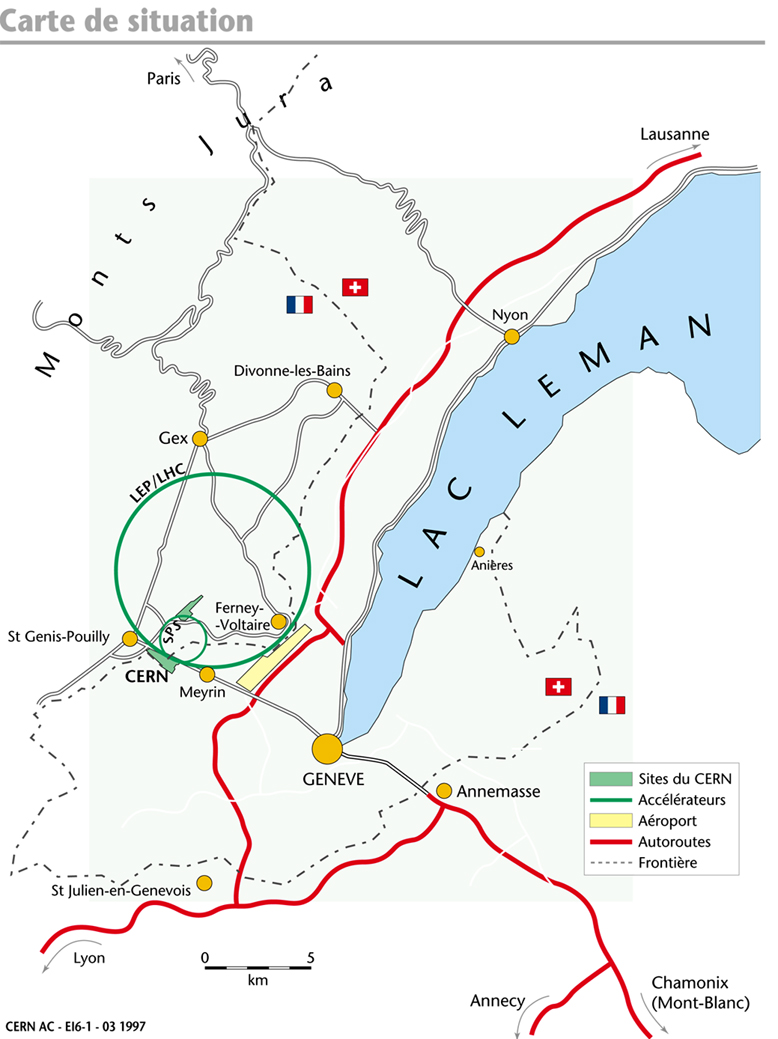
\includegraphics[width=0.6\textwidth]{Chapters/01_Introduction/Images/lhc-pho-1997-169.jpg}\\
     \caption{Map of LHC location.}
     \label{fig:LHC_map}
\end{figure}

This thesis presents an analysis based on the full proton-proton collision data from the CMS experiment in
2011 and 2012. The analysis investigates the top-antitop (\ttbar) differential cross section with respect to
global level event variables, specifically in semileptonic \ttbar decays in the electron+jets and muon+jets
channels. This investigation is motivated primarily by the importance of understanding \ttbar events, since
they are a significant background in many new physics analyses. The understanding of QCD and event generators
that studies such as this provide is also helpful for other physics analyses. Furthermore, rare Standard Model
processes such as $\ttbar + W\rightarrow l\nu$ or $\ttbar + Z\rightarrow \nu\bar{\nu}$ would appear in \met
distribution tail, and $\ttbar + X$ where $X$ is massive would appear in the \HT and \st distributions. There
are also possible new physics scenarios such as stop pair production, $\tilde{t}\bar{\tilde{t}} \rightarrow
t\tilde{\chi_0} \bar{t}\bar{\tilde{\chi_0}}$ which could show hints of dark matter.

The work presented here was carried out in collaboration with Emyr Clement, L{}ukasz Kreczko, Sergey Senkin
and Philip Symonds under the supervision of Professors Joel Goldstein and Greg Heath. The main contribution of
the author to these studies lay in development of the C++ and Python software frameworks and scripts used in
the analyses. Related to this, maintaining up-to-date particle object definitions, corrections, efficiencies
and prescription recommendations from working groups within CMS was a large component of the author's work. In
terms of the technical workflow employed, the author was heavily involved in producing n-tuples from the
analysis-ready AOD data format, running the software to perform the prescribed analysis methods, and running
final scripts on the output ROOT data to perform the final calculation and to produce results plots and
tables. Particular areas of focus regarding physics included synchronisation of the event selection,
comparison of distribution shapes between 7\TeV and 8\TeV data, and implementing aspects of the analyses such
as selection criteria, \btagging and jet energy resolution.

Chapters~\ref{c:CMS_Detector} and \ref{c:CMS_computing_and_offline} describe the LHC and the CMS detector,
including information about the object reconstruction process based on detector readout, to represent
particles produced in collisions. Chapter~\ref{c:the_standard_model} provides an overview of the Standard
Model theory and some of its shortcomings, followed by a review of physics of the top quark at the LHC in
Chapter~\ref{c:top_physics_at_the_lhc}. A small study investigating the \btagging algorithms used in CMS is
described in Chapter~\ref{c:b_tagging_study}, and the main \ttbar differential cross section analysis is then
covered in Chapters~\ref{c:Differential_Cross_Section:data_simulation_and_selection},
\ref{c:Differential_Cross_Section:fitting_unfolding_and_measurement}
and~\ref{c:Differential_Cross_Section:systematics_and_results}. To conclude, Chapter~\ref{c:summary} contains
a summary and outlook to the future. Additional data, tables and plots from the presented analyses are given
in Appendices~\ref{ac:b_tagging_plots} and \ref{ac:ttbar_diff_cross_section_analysis}. Finally, an addendum
describing the brief continuation of work from the author's MSc in testing a readout chip for the CMS strip
tracker is outlined in Appendix~\ref{ac:cbc}.

From the outset, natural units are used throughout this thesis, unless otherwise specifed, so that
\begin{equation}
\hbar = c = 1,
\end{equation}
meaning that mass, momentum and energy all have the same units of electronVolts (eV).
\chapter{The Standard Model}
\label{c:the_standard_model}

The top quark was discovered by the CDF and D{\O} collaborations in 1995 and is still one of the less
well studied fundamental particles in the Standard Model. The top quark is the heaviest fermion with its mass
currently placed at $173.29 \pm 0.23 (stat.) \pm 0.92 (syst.)~GeV/c^{2}$ \cite{top_mass}. Since the lifetime
of the top quark is very short, approximately $5 \times 10^{25}~s$, it is the only one of the quarks to decay
before it hadronises, meaning that the bare quark properties can be investigated. These unique properties of
the top quark within the Standard Model mean it is an interesting focus of study.

During 2011 and 2012, the LHC produced millions of top quark pair events with gluon-gluon fusion (\~70\%) or
quark\-anti\-quark annihilation (\~30\%) TODO:feynmann diagram of production mechanisms %TODO:FEYNMANN DIAGRAM OF PRODUCTION MECHANISMS
being the primary production mechanisms. Top quarks decay almost 100\% of the time to a W-boson and a b
flavour jet. The W-boson then decays either hadronically (into two jets) or leptonically (lepton + neutrino).
Top pair events are characterised by the decay of the W-bosons:
\begin{itemize}
  \item Leptonic - both W-bosons decay to a lepton and a neutrino. The event would consist of 6 jets. (10.5\%)
  \item Hadronic - both W-bosons decay to two jets. The event would consist of 2 jets, 2 leptons and 2
  neutrinos (which would show up as \met in the event). (45.7\%)
  \item Semi-Leptonic - one W-boson decays to a lepton and a neutrino, the other decays to two jets. The
  event would consist of 4 jets, 1 lepton and 1 neutrino. (43.8\%)
\end{itemize}

The branching ratios for each decay mode are quoted in brackets \cite{PDG}, and are represented graphically in
Figure~\ref{fig:ttbar_branching_ratios}.

\begin{figure}[hbtp]
   \centering
     \includegraphics[width=0.5\textwidth]{Chapters/02_Theory/Images/top_pair_decay_channels.eps}\hfill
     \caption{Relative branching ratios of the \ttbar system}
     \label{fig:ttbar_branching_ratios}
\end{figure}


\section{ttbar Signal and Background processes}
- signal
- single top
- W plus jets
- Z + jets
- QCD

- theory systematics (factorisation scale and matching threshold)

(see L p. 86 onwards)

Gluon-gluon fusion contributes more at the LHC as a result of the gluon momentum fraction increasing at a
higher rate than that carried by the sea quarks which would be required to produce a top pair.

\section{Monte Carlo Simulation}
\label{s:monte_carlo_simulation}
\subsection{Generators}
\label{ss:generators}
- Madgraph
- Pythia
- Powheg

\subsection{Factorisation \& Matching Threshold}
\label{ss:factorisation_and_matching_threshold}

\subsection{Detector Simulation (GEANT)}
\label{ss:detector_simulation}

\chapter{Top Physics at the LHC}
\label{c:top_physics_at_the_lhc}

\section{Introduction}
\label{s:top_physics_intro}
The top quark was discovered by the CDF and D{\O} collaborations at the Tevatron at Fermilab in 1995
\cite{Abe:1995hr, Abachi:1995iq} and is still one of the less well studied fundamental particles in the
SM. The top quark is the heaviest fermion with its mass currently placed at $173.29\pm0.23
(\stat)\pm0.92(\syst)\GeV/c^{2}$~\cite{top_mass}. Since the lifetime of the top quark is very short,
approximately $5\times10^{-25}\s$~\cite{Agashe:2014kda}, it is the only one of the quarks to decay
before it hadronises, meaning that the bare quark properties can be investigated. These unique properties of
the top quark within the SM mean it is an interesting focus of study.

\subsection{Top Quark Production and Decay}
\label{ss:top_quark_production_and_decay}
Top quarks can be produced either in top-antitop (\ttbar) production through the strong interaction or single
top (\tquark) production through the electroweak mechanism. During Run~1 of data taking at the LHC produced
millions of top quark pair events with gluon-gluon fusion or quark-antiquark annihilation being the primary
production mechanisms (shown in Figure~\ref{fig:ttbar_production}). The \ttbar production cross section at
$\sqrt{s}=1.96\TeV$ was measured by the CDF and D{\O} collaborations at the TeVatron, while the cross sections
at $\sqrt{s}=7\TeV$ and $\sqrt{s}=8\TeV$ have been measured by CMS and ATLAS at the LHC. The measurements are
summarised in Figure~\ref{fig:ttbar_cross_sections_plot}. Numerical cross sections values at the LHC, at
\roots=7\TeV, \roots=8\TeV, \roots=13\TeV and \roots=14\TeV are shown in
Table~\ref{tab:ttbar_and_single_top_cross_sections}.

\begin{figure}[hbtp]
   \centering
     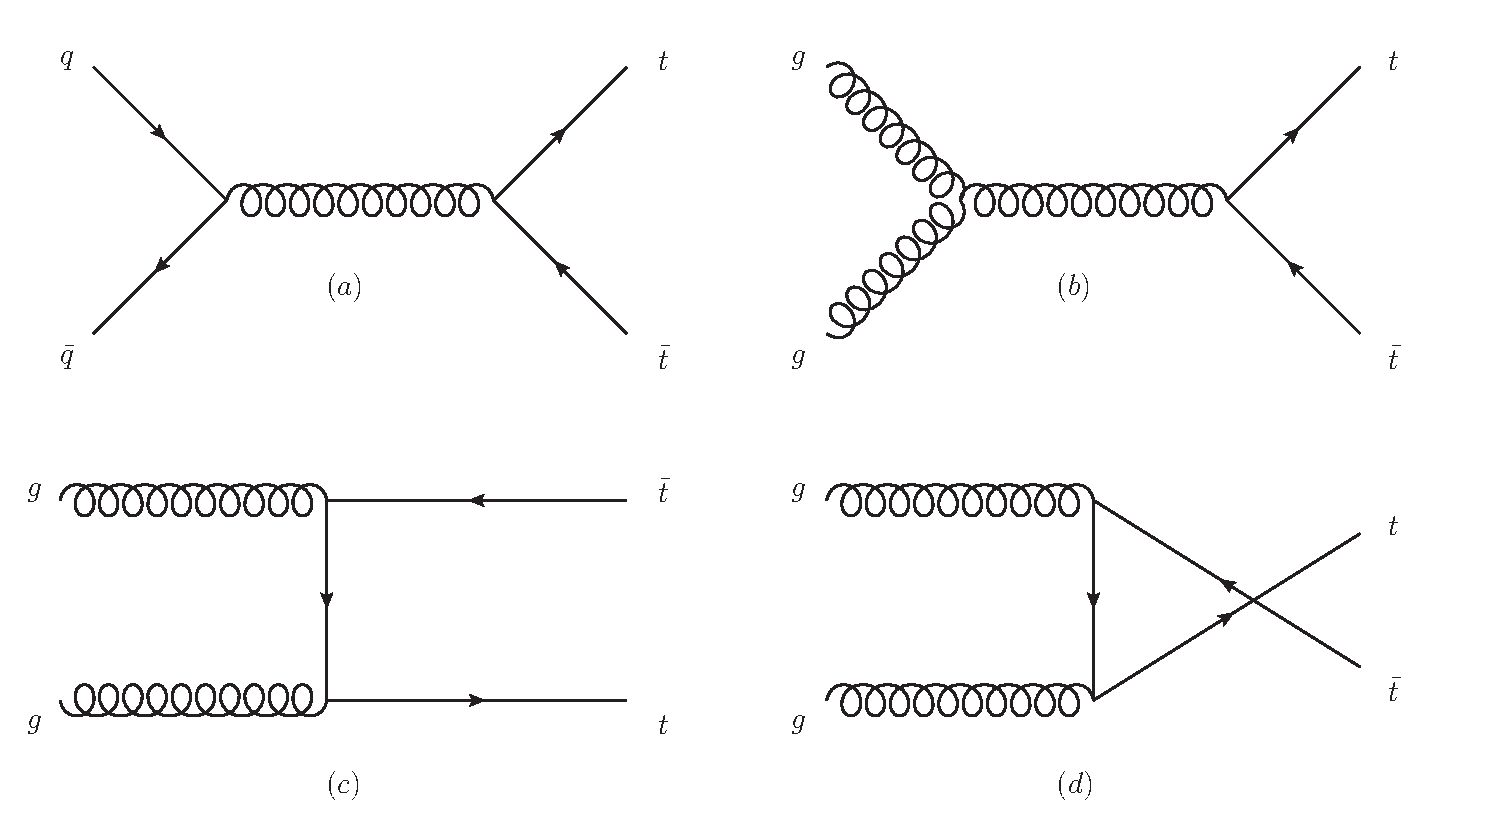
\includegraphics[width=0.9\textwidth]{Chapters/03_Top_Physics/Images/ttbar_production}\hfill
     \caption[Feynman diagrams of leading order \ttbar production processes.]{Feynman diagrams of leading
     order \ttbar production processes. (a) depicts quark-antiquark annihilation, and (b), (c) and (d) depict
     gluon-gluon fusion in the s, t and u channels respectively.)}
     \label{fig:ttbar_production}
\end{figure}

\begin{figure}[hbtp]
   \centering
     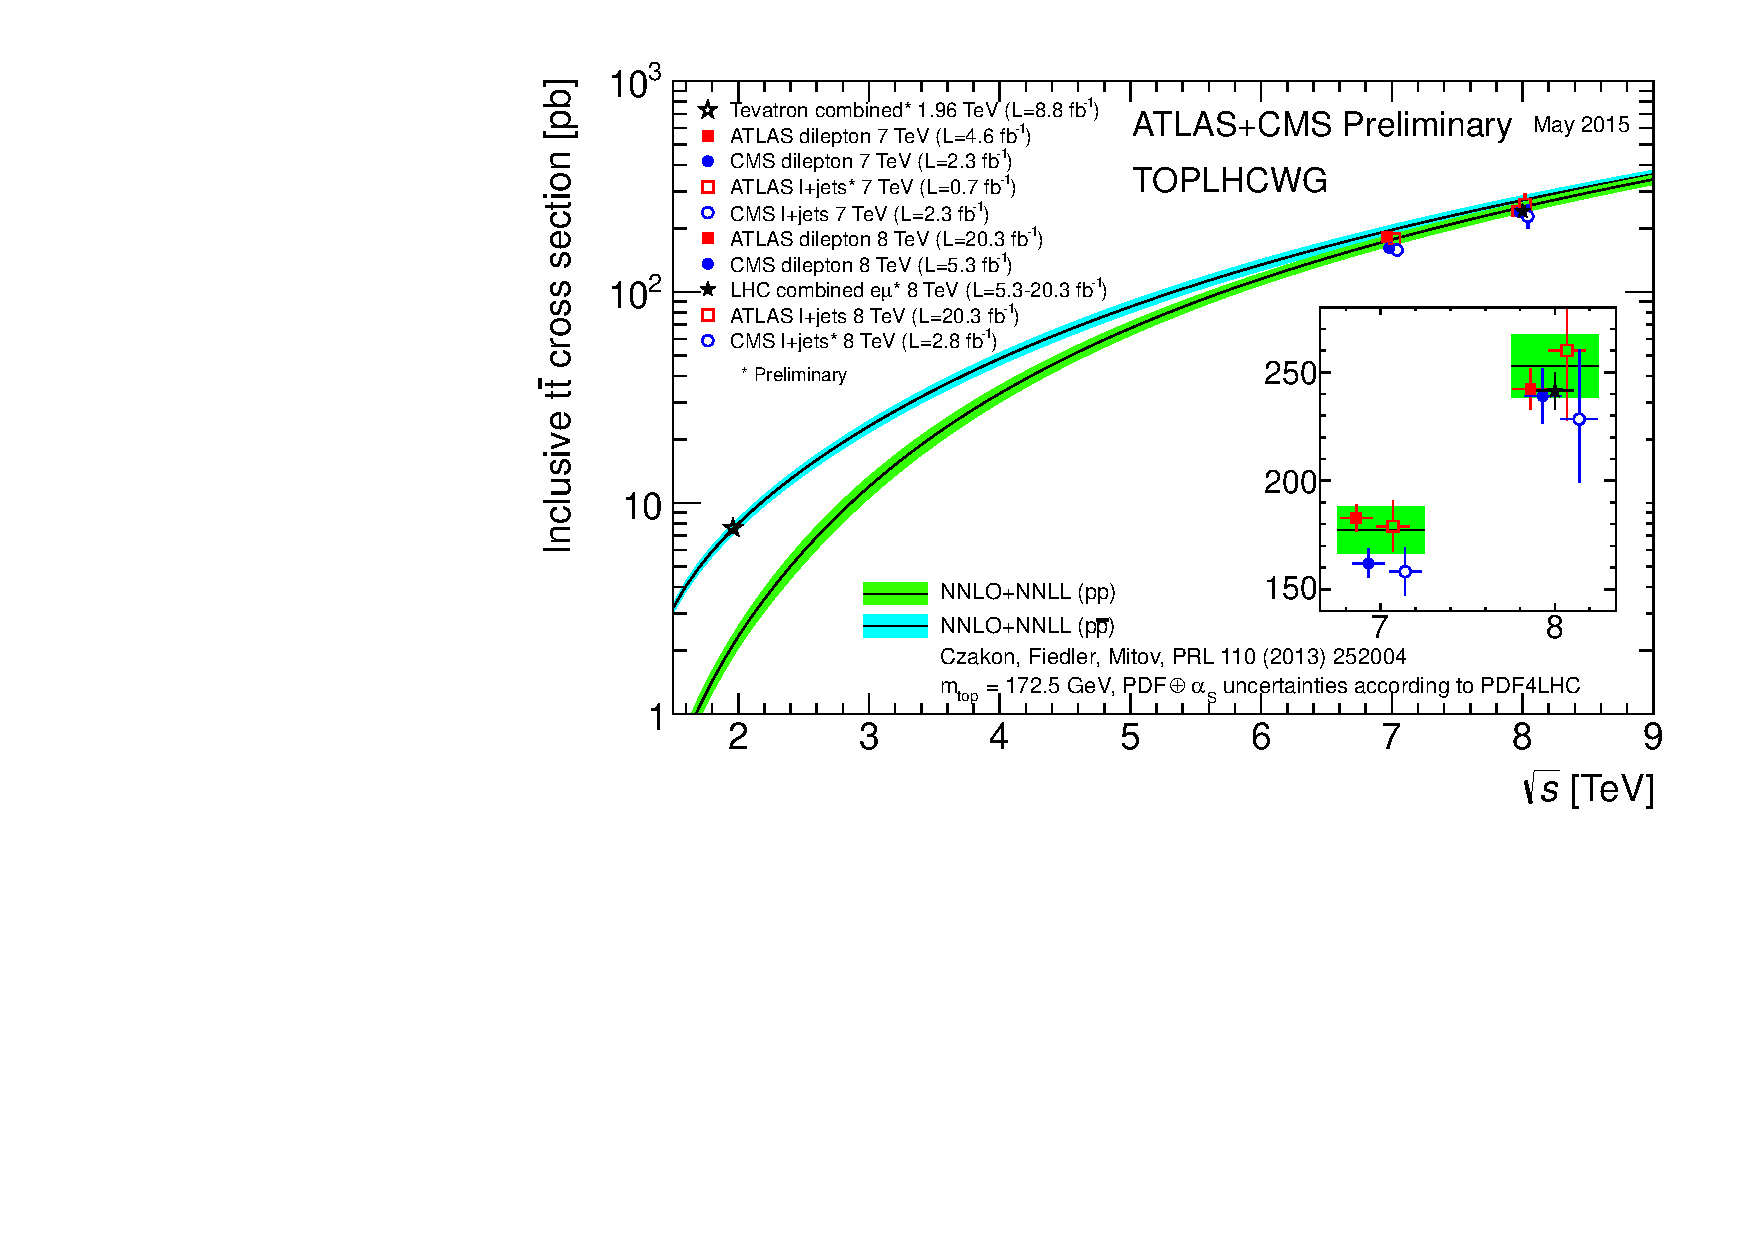
\includegraphics[width=0.8\textwidth]{Chapters/03_Top_Physics/Images/toplhcwg_ttxsec_sqrts_may2015}\hfill
     \caption[\ttbar production cross sections at 1.96\TeV at CDF and D{\O} at the TeVatron and at 7\TeV and
     8\TeV at CMS and ATLAS at the LHC.]{\ttbar production cross sections at 1.96\TeV at CDF and D{\O} at the
     TeVatron and at 7\TeV and 8\TeV at CMS and ATLAS at the LHC~\cite{TOPLHC_WG}.}
     \label{fig:ttbar_cross_sections_plot}
\end{figure}

\begin{table}[hbth]
\centering
\resizebox{\columnwidth}{!} {
\begin{tabular}{|r|r|r|r|r|}
\hline
\roots & \ttbar & Single \cPqt s-channel & Single \cPqt t-channel & Single \cPqt tW-channel \\
\hline
%1.96
7  & 177.31 & 4.29 & 63.69 & 15.74 \\
8  & 252.89 & 5.24 & 84.69 & 22.37 \\
13 & 831.76 & 10.32 & 216.99 & 71.70 \\
14 & 984.50 & 11.39 & 248.09 & 84.40 \\
\hline
\end{tabular}
}
\caption{SM \ttbar and single top production cross sections in \pb at next-to-next-to-leading order at the
LHC.}
\label{tab:ttbar_and_single_top_cross_sections}
\end{table}

At the TeVatron, quark-antiquark annihilation dominated, accounting for 90~\% of the \ttbar production cross
section. At $\sqrt{s}=7\TeV$, gluon-gluon fusion accounts for approximately 80~\% of the \ttbar production,
increasing to approximately 90~\% at $\sqrt{s}=14\TeV$ \cite{Agashe:2014kda}. Gluon-gluon fusion dominates at
the LHC since protons are collided with protons, meaning antiquarks are only available from sea quarks in the
proton. At low momentum fractions, $x$, the gluon density in the proton is large compared to the sea quarks,
and increases towards lower $x$ at a higher rate than that of the sea quarks.
Figure~\ref{fig:proton_parton_pdfs} shows the proton parton distribution functions (PDFs) at a momentum
transfer, $Q^{2}=10000\GeV^{2}$, the region relevant for the LHC and of the order required for \cPqt/\W/\Z
production. At low $x$, it can be seen that the sea quarks and gluons dominate, while the valence quarks
increase in number at high $x$.

\begin{figure}[hbtp]
   \centering
     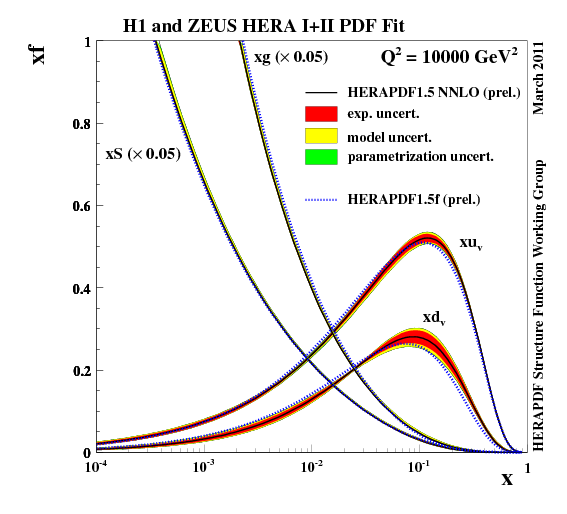
\includegraphics[width=0.7\textwidth]{Chapters/03_Top_Physics/Images/proton_pdfs}
     \hfill
     \caption[Proton parton distribution functions at $Q^{2}=10\GeV^{2}$.]{Parton distribution functions from
     HERA as a function of proton momentum fraction for $Q^{2}=10\GeV^{2}$~\cite{Placakyte:2011az}.}
     \label{fig:proton_parton_pdfs}
\end{figure}

Top quarks decay almost 100~\% of the time to a \W boson and a \cPqb flavour jet. The \W boson then decays
either hadronically (into two jets) or leptonically (lepton + neutrino). Top pair events are characterised by the
decay of the \W bosons:

\begin{itemize}
  \item Leptonic: $\ttbar \rightarrow \W^{+} \cPqb \W^{-} \cPaqb \rightarrow l \nu_{l}\cPqb
  l' \bar{\nu_{l'}} \cPaqb$.
  Both \W bosons decay to a lepton and a neutrino. The event would consist of 2 jets, 2 leptons and 2
  neutrinos (which would show up as missing transverse energy (\met) in the event). (10.5~\%)
  \item Hadronic: $\ttbar \rightarrow \W^{+} \cPqb \W^{-} \cPaqb \rightarrow \cPq \cPaq \cPqb \cPq \cPaq
  \cPaqb$. Both \W bosons decay to two jets. The event would consist of 6 jets. (45.7~\%)
  \item Semi-Leptonic: $\ttbar \rightarrow \W^{+} \cPqb \W^{-} \cPaqb \rightarrow \cPq \cPaq \cPqb l \nu_{l}
  \cPaqb$. One \W boson decays to a lepton and a neutrino, the other decays to two jets. The event would
  consist of 4 jets, 1 lepton and 1 neutrino. This decay is shown in Figure~\ref{fig:semileptonic_decay}.
  (43.8~\%)
\end{itemize}

\begin{figure}[hbtp]
   \centering
     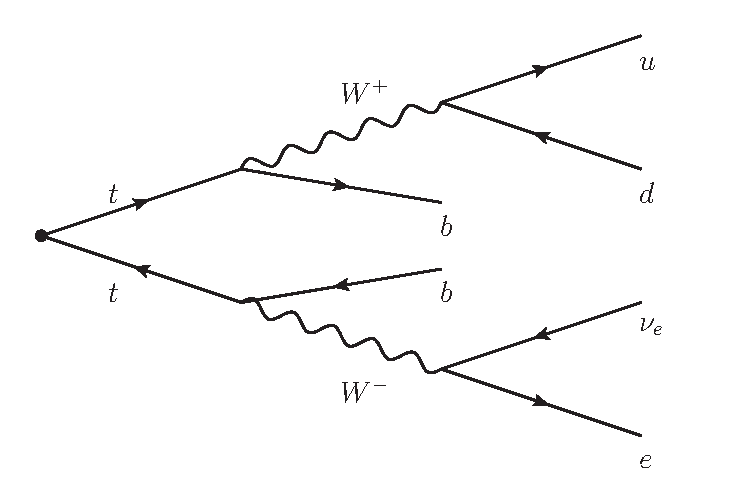
\includegraphics[width=0.7\textwidth]{Chapters/03_Top_Physics/Images/semileptonic_decay}\hfill
     \caption[Feynman diagram of the electron+jets semi-leptonic \ttbar decay channel.]{Feynman diagram of the
     electron+jets semi-leptonic \ttbar decay channel.}
     \label{fig:semileptonic_decay}
\end{figure}

The branching ratios for each decay mode are quoted in brackets \cite{Agashe:2014kda}, and are represented
graphically in Figure~\ref{fig:ttbar_branching_ratios}. The numbers of jets in the final state of each channel
could be higher than the numbers quoted above as a result of higher order processes such as initial state
radiation (radiation from the gluons before the \ttbar production) or final state radiation. The hadronic
decay channel, with multiple jets and no leptons in the final state, is difficult to distinguish from the QCD
multijet, W+jets and Z+jets backgrounds. Conversely, the leptonic channel has a very clean signature with two
leptons, however the low branching ratio would limit the available statistics. The semi-leptonic channel, with
one lepton and four jets provides a good balance between statistics and event identification. The lepton can
be an electron, a muon or a tau. However, top events with taus are difficult to distinguish from genuine
semi-leptonic events, hence resulting measurements are generally less precise, and therefore taus are not
included in semi-leptonic \tquark studies in general (see Section~\ref{ss:experimental_uncertainties} for more
details regarding taus in semi-leptonic \ttbar events).

\begin{figure}[hbtp]
   \centering
     \includegraphics[width=0.5\textwidth]{Chapters/03_Top_Physics/Images/top_pair_decay_channels}\hfill
     \caption[Relative branching ratios of the \ttbar system]{Relative branching ratios of the \ttbar system}
     \label{fig:ttbar_branching_ratios}
\end{figure}

The signal channel for the analysis described in this work is semi-leptonic \ttbar decay, also referred to as
the lepton+jets channel, where the lepton is either an electron or a muon. These channels have a branching
ratio of approximately 14.2~\% and 14.4~\% respectively~\cite{Agashe:2014kda}.

\subsection{Single Top background}
\label{ss:single_top}
Single top production is one of the backgrounds considered in this analysis, and can occur via the electroweak
interaction in one of three channels: s-channel (Figure~\ref{fig:single_top_production} (a)), t-channel
(Figure~\ref{fig:single_top_production} (b) and (c)) which both involve the exchange of a virtual \W boson, or
\tW-channel (Figure~\ref{fig:single_top_production} (d) and (e)) which involves the associated production of a
\W boson and a top quark. Although semi-leptonic \ttbar decays have more jets in the final state than these
single top production modes, initial state radiation and final state radiation, where low energy gluons and
quarks are produced before and/or after the interaction that produces the single \tquark, can increase the
numbers of jets in single top events. This can lead to such events having a similar signature to \ttbar
events, and providing a non-negligble background. SM production cross sections for single top events are shown
in Table~\ref{tab:ttbar_and_single_top_cross_sections}. Comparisons of data to Monte Carlo simulation, and the
composition of the backgrounds, including single top events, will be shown in
Section~\ref{ss:data-mc_comparison}.

\begin{figure}[hbtp]
   \centering
     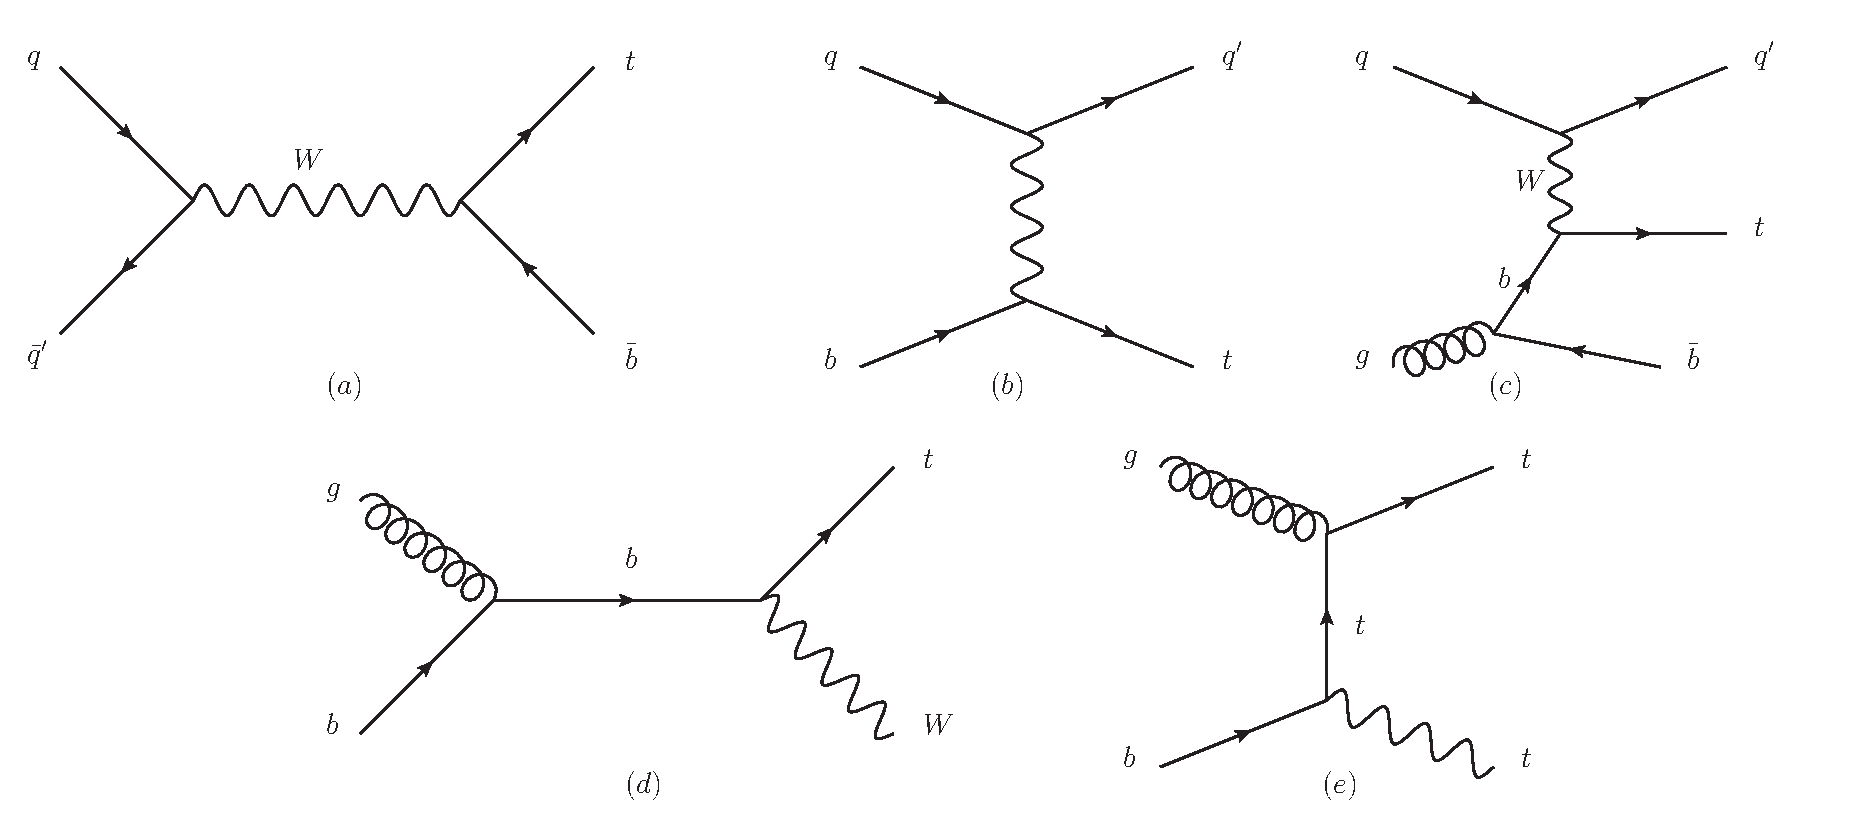
\includegraphics[width=0.9\textwidth]{Chapters/03_Top_Physics/Images/single_top_production}\hfill
     \caption[Feynman diagrams of leading order single top production processes.]{Feynman diagrams of leading
     order single top production processes in the s-channel (a), t-channel (b) and (c), and associated tW
     production (d) and (e).}
     \label{fig:single_top_production}
\end{figure}

\subsection{W/Z+jets background}
\label{ss:w_z_plus_jets}
\WpJets production presents a significant background to semi-leptonic \ttbar analyses. This background
consists of events in which a real \W boson is produced together with additional jets. Events in which these
\W bosons decay leptonically can provide a similar event signature after reconstruction to that of a
semi-leptonic \ttbar decay. In general, these processes can be removed from the signal selection because the
final decay products in \WpJets events typically have lower energies than those from semi-leptonic \ttbar
decays, since the top quark has a high mass. Another characteristic of \WpJets events is that the jets are
more likely to be light quark jets and therefore less likely to be \bjets than in \ttbar events. Thus, \WpJets
events can be separated to a large extent from the \ttbar signal by using jet multiplicity, jet \pt and \bjet
multiplicity.

Similarly, \ZpJets events can mimic \ttbar events where the leptonic decay of a \Z boson to a lepton and an
anti-lepton takes place. This background can be distinguished from semi-leptonic \ttbar decays by
vetoing on a second lepton and imposing jet multiplicity requirements. Misidentification and misreconstruction
of these leptons as jets, however, can result in such events mimicking \ttbar events and passing the signal
selection, although this contamination is small. Comparisons of data to Monte Carlo simulation, and the
composition of the backgrounds, including \WpJets and \ZpJets events, will be shown in
Section~\ref{ss:data-mc_comparison}.

\subsection{QCD background}
\label{ss:qcd}
The multijet background from QCD events presents a significant obstacle in many measurements at LHC, including
this semi-leptonic \ttbar analysis. Gluon-gluon fusion and quark-antiquark annihilation in proton-proton
collisions can produce energetic jets. Although these processes have only two jets in their final state,
higher order processes, including initial state radiation and final state radiation, can also produce
additional jets, leading to potential mimicking of the semi-leptonic \ttbar signal. The leptons required for
this to happen can come from jets which are misreconstructed and misidentified as leptons, or real leptons in
heavy flavour (\cPqb and \cPqc) jets. Unfortunately the cross section of these processes is several orders of
magnitude larger than the signal cross section. Although the lepton (either fake or real) is rarely one that
passes selection, the much higher QCD cross section means that its contribution as a background is
significant.

In the muon+jets channel, only highly energetic jets ($\pt>500\GeV$) are capable of ``punching through'' from
the calorimeters to leave tracks in the muon chambers. Such events can be removed by isolation requirements
(since they deposit significant amounts of energy in the calorimeters). Events with real electrons and muons
from heavy quark jets can be identified by the track quality requirements in the selection since they would
not begin from the primary vertex and so would have a distinct track signature compared to prompt leptons.

On the other hand, the electron channel poses a more problematic QCD background, due mainly to the conversion
of photons, whether produced at the interaction point or through subsequent decays and radiation, into
electrons and positrons. The identification and removal of such events is described in
Section~\ref{ss:electron_reconstruction}. However, the large uncertainty in the cross sections of QCD events,
large contamination from higher order processes with additional jets in the signal region of this analysis and
the difficulty in modelling such contributions, lead to incorrect event kinematics and significant
disagreements in the QCD background distributions in data and in simulation. Therefore, the QCD background is
modelled using a data driven method, described in Section~\ref{ss:background_selection}, and then normalised
to the number of events passing the signal selection in simulation. Comparisons of data to Monte Carlo
simulation, and the composition of the backgrounds, including QCD multi-jet events, will be shown in
Sections~\ref{ss:background_selection} and~\ref{ss:data-mc_comparison}.

\section{Monte Carlo Simulation}
\label{s:monte_carlo_simulation}

Monte Carlo event simulation is used to simulate the aforementioned signal and background processes, and to
compare the theoretical knowledge of the SM incorporated therein with real data. Differences
between simulation and data would then indicate the presence of new physics processes which are not present in
the theoretical assumptions made in the SM, or perhaps that the simulation process is sub-optimal.
Different event generators exist, and samples produced by the \MADGRAPH, \PYTHIA, \POWHEG and \HERWIG
generators are used in this analysis.

Different generators have characteristics which optimise them for different aspects of the production chain:
the initial hard process scattering of the partons in the hadrons (protons), decay showers of the resulting
partons, subsequent decays of resulting hadrons and hadronisation of resulting partons, and the underlying
event (the parton showers produced from soft scattering between the remaining contents of the colliding
protons). 

\subsection{MadGraph}
\label{ss:madgraph}
\MADGRAPH \cite{madgraph5}, a matrix element generator, works by taking into account leading-order (LO)
Feynman diagrams for a given process and subsequently calculating the matrix elements for these diagrams with
up to three additional partons, over all phase space. The PDFs are used to generate the incoming partons. The
cross section of the process and various subprocesses and the structure and contents of the event (such as the
partons present and their kinematics) are thus produced. Proton fragmentation and subsequent hadronisation are
simulated using the \PYTHIA generator, as explained in Section~\ref{ss:pythia}.

The \PYTHIA parton showers are then matched with the matrix element partons via the MLM
method~\cite{Hoche:2006ph}. This method ensures that parton showers with a highly energetic jet are not double
counted. Matching is carried out between parton showers in the hadronisation and the partons from the matrix
element calculations. The matching is carried out by satisfying distance requirements in $\eta$ and $\phi$
between the parton and parton shower. Only if the parton has a transverse energy above a certain threshold, is
it considered for this matching, and if an event contains either too few or too many matching jets, it is
discarded. The matching threshold is process dependent as follows:

\begin{itemize}
  \item \ttbar: 20\GeV
  \item \WpJets: 10\GeV
  \item \ZpJets: 10\GeV
\end{itemize}

\subsection{MC@NLO}
\label{ss:mcatnlo}
The \MCATNLO~\cite{Frixione:2002ik,Frixione:2003ei} generator is a next-to-leading-order (NLO) generator.
These additional corrections provide more accurate simulations of physics processes in comparison to LO
generators by including additional partons from the initial hard process in the final state of the event.

\subsection{PYTHIA}
\label{ss:pythia}
\PYTHIA~\cite{Sjostrand:2006za} then simulates the proton fragmentation, the subsequent hadronisation of the
resulting quarks and gluons resulting from the hard interaction and the underlying event. \PYTHIA is considered to be
particuarly good at multi-particle simulation, modelling fragmentation and hadronisation. Therefore, \PYTHIA
carries out these steps after the initial partons are provided by other generators in most simulated samples,
if it is not already used for the whole production chain (as is common in QCD multijet simulations).

\subsection{POWHEG}
\label{ss:powheg}
One problem with the \MCATNLO generator is that some events are given negative weights when matching the NLO
QCD multijet calculations to parton showers.  The Positive Weight Hardest Emission Generator,
\POWHEG~\cite{Frixione:2007vw,Nason:2004rx,Alioli:2010xd}, is another NLO generator which generates the
hardest processes in the event first, which avoids double counting of softer radiation produced later in the
chain, which is the cause of negative event weights.

%\subsection{HERWIG}
%\label{ss:herwig}
%\HERWIG \cite{herwig}
%TODO:HERWIG

\section{Theoretical Systematics}
\label{s:Theoretical Systematics}
\subsection{Factorisation and Renormalisation Scale \& Matching Threshold}
\label{ss:factorisation_and_matching_threshold}
The models used in generators use an essentially arbitrary choice for the threshold transverse energy above
which matrix-element partons are matched to parton showers. To account for the systematic uncertainties as a
result of this threshold, simulated samples in which this matching threshold is increased and decreased by a
factor of 2 (see Table~\ref{tab:matching_factorisation_uncertainty}) are used to estimate the effect of this
uncertainty on this analysis.

Similarly, the factorisation ($\mu_{\mathrm{F}}$) and renormalisation ($\mu_{\mathrm{R}}$)scale, or $Q^{2}$,
at which $\alpha_{S}$ is evaluated, is varied up and down from the nominal value of $Q^{2} = m^{2} + \Sigma
p_{T}^{2}$ by a factor of 2 (see Table~\ref{tab:matching_factorisation_uncertainty}) to produce simulation
samples to evaluate the systematic uncertainty resulting from this. The uncertainty resulting from these
variations in both \ttbar and \W/\ZpJets processes is evaluated.

\begin{table}[hbth]
\centering
\resizebox{\columnwidth}{!} {
\begin{tabular}{|l|ccc|ccc|}
\hline
 & \multicolumn{3}{c}{Matching Threshold} & \multicolumn{3}{c}{Factorisation Scale} \\
Process & nominal / \GeV & + variation / \GeV & - variation / \GeV & nominal / \GeV & + variation / \GeV &  -
variation \\
\hline
\ttbar & 20 & 40 & 10 & $Q^{2} = m_{T}^{2} + \Sigma p_{T}^{2}$ & $(2Q)^{2}$ & $(0.5Q)^{2}$ \\
\WpJets & 10 & 20 & 5 & $Q^{2} = m_{W}^{2} + \Sigma p_{T}^{2}$ & $(2Q)^{2}$ & $(0.5Q)^{2}$ \\
\ZpJets & 10 & 20 & 5 & $Q^{2} = m_{Z}^{2} + \Sigma p_{T}^{2}$ & $(2Q)^{2}$ & $(0.5Q)^{2}$ \\
\hline
\end{tabular}
}
\caption{Threshold transverse energy for matching systematic uncertainty}
\label{tab:matching_factorisation_uncertainty}
\end{table}

\subsection{Detector Simulation (GEANT)}
\label{ss:detector_simulation}
Following creation of the physics processes in proton-proton collisions, the simulated events are then put
through a detector simulation to evaluate the interaction of the detector with the products of collisions. The
Geometry and Tracking (\GEANT) package~\cite{Agostinelli:2002hh,Allison:2006ve} is used for this
purpose, which simulates what happens to particles as they travel through the geometry of the detector,
including simulation of the detector components and materials and the interaction of particles with the
detector such as particle tracks and energy deposits.
\chapter{The CMS Detector at the LHC}
\label{c:CMS_Detector}

\section{Introduction to the LHC}
\label{s:Introduction}
The CMS general-purpose detector is one of four detectors located around the LHC, approximately 100\m below
ground level. The CERN accelerator complex and the locations of the various experiments around the LHC are
shown in Figure~\ref{fig:LHC_schematic}.

\begin{figure}[hbtp]
   \centering
     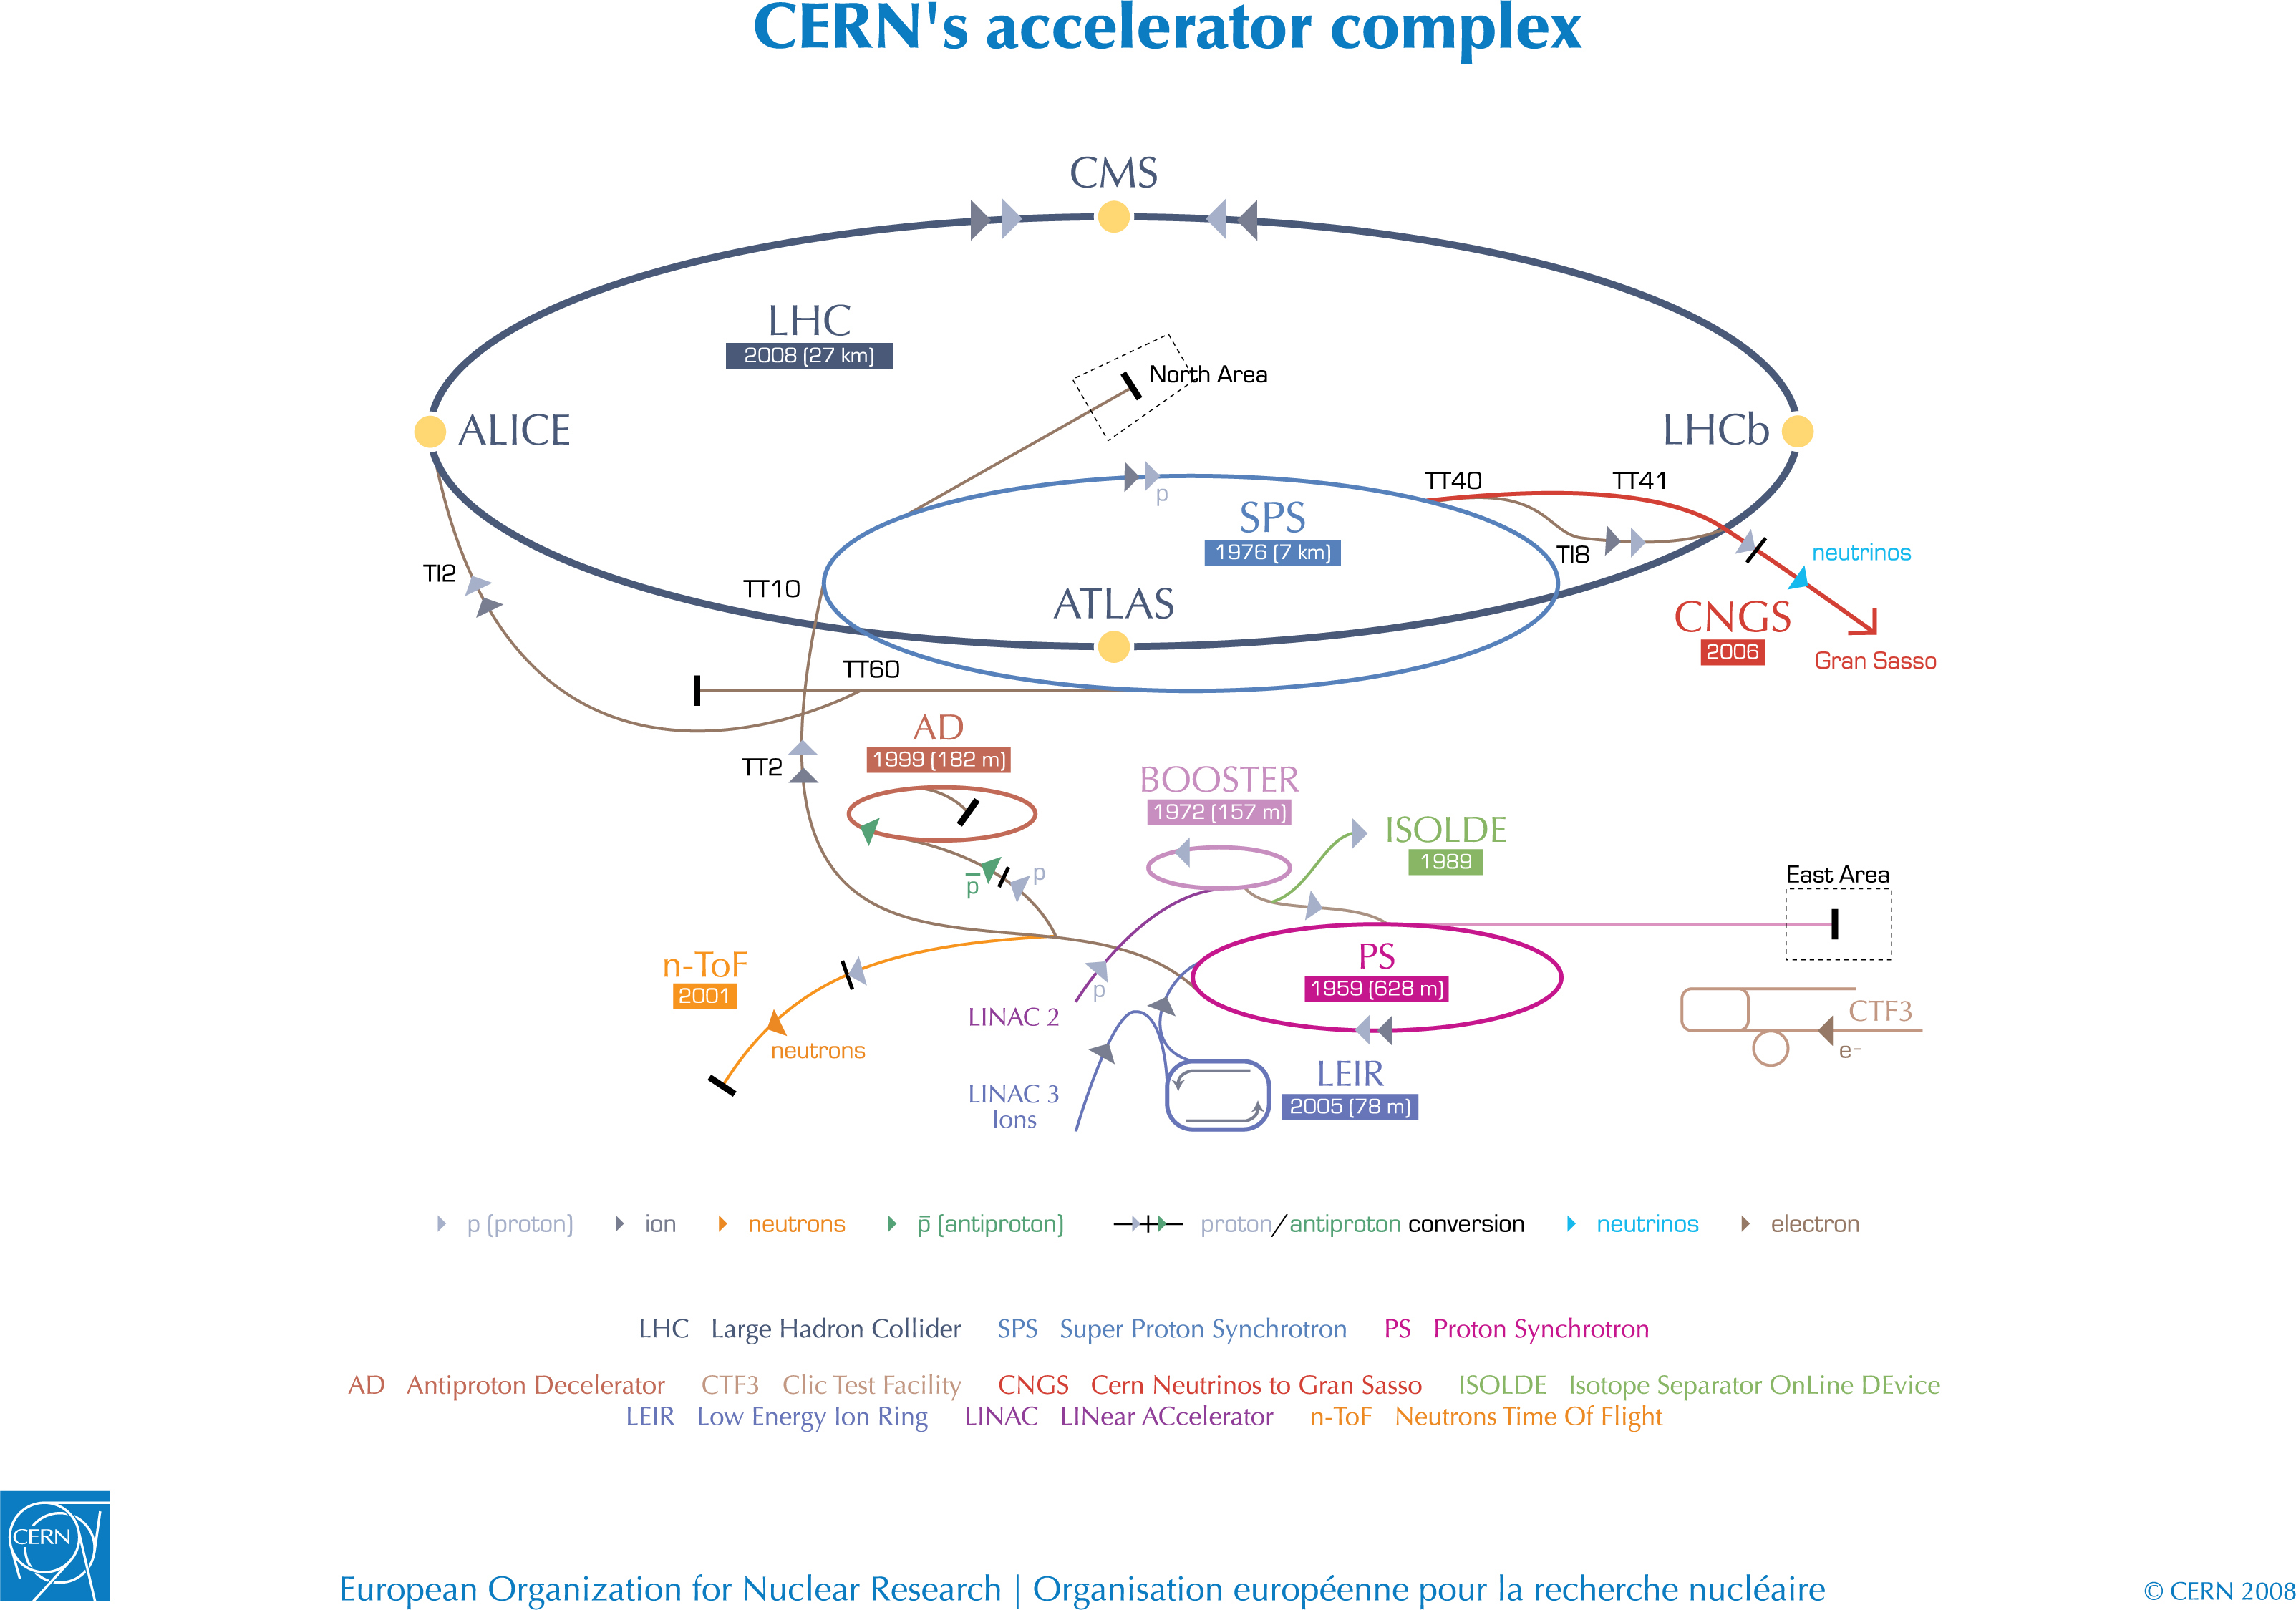
\includegraphics[width=\textwidth]{Chapters/04_Detector/Images/0812015.jpg}\\
     \caption[Schematic of LHC and experiments.]{Schematic of CERN accelerator complex including the LHC and
     experiments.
     CMS is located at Point 5 on the LHC ring.}
     \label{fig:LHC_schematic}
\end{figure}

The 27\km circumference LHC is designed to collide two proton beams, each composed of 2808 bunches, at a
design energy of 7\TeV per beam (meaning a 14\TeV centre-of-mass energy, \roots, in collisions) with a
luminosity $\mathcal{L}$ of $10^{34}\cm^{-2}\s^{-1}$ at a collision rate of 25\ns (40~\MHz). Each event that
is recorded in the CMS detector is one crossing of the bunches of protons of which the beams are comprised.
During the first part of Run 1 in 2011 the machine ran at a centre-of-mass-energy of 7\TeV at a bunch spacing
of 50\ns (leading to 8 proton-proton interactions per bunch crossing) and CMS recorded a peak instantaneous
luminosity of $3.7\times10^{33}\cm^{-2}\s^{-1}$. In 2012 the centre-of-mass energy was increased to 8\TeV (21
proton-proton interactions per bunch crossing) and CMS recorded a peak instantaneous luminosity of
$7.7\times10^{33}\cm^{-2}\s^{-1}$. Since Run 2 began in May 2015 after Long Shutdown 1, the LHC has been
operating at a collision energy of 13\TeV and CMS recorded a peak instantaneous luminosity of
$4.7\times10^{33}\cm^{-2}\s^{-1}$ at a collision rate of 25\ns initially, before switching to 50\ns.
The design collision energy and luminosity are scheduled to be attained later in Run 2 and after Long Shutdown
2 (in 2019) respectively. 6.1\fbinv and 23.3\fbinv of data was delivered to CMS during the 2011 and 2012 data
taking periods respectively; Figure~\ref{fig:integrated_luminosity} shows the increase in integrated
luminosities delivered to CMS over time during 2010\textendash2012.

The acceleration process, or fill, begins with a tank of hydrogen (see Figure~\ref{fig:LHC_schematic}). After
stripping electrons off the hydrogen atoms using an electric field, the remaining protons are inserted into the Linear
Accelerator 2 (LINAC2) which accelerates them up to 50\MeV. From here, the proton beam is injected into the
Proton Synchrotron Booster (PSB) which increases the energy to 1.4\GeV, followed by the Proton Synchrotron
(PS) which accelerates the beam to 25\GeV and the Super Proton Synchrotron (SPS) where the beam energy reaches
450\GeV. Finally, the protons are injected into the LHC where two beampipes carry the beams in a clockwise and
an anti-clockwise direction while accelerating them up to the required collision energy. Filling the LHC rings
takes approximately 4 minutes, followed by approximately 20 minutes until the beams reach energies of 4\TeV
(during 2012 data taking). The beams are accelerated by radio frequency cavities, and superconducting dipole
magnets bend the beams to maintain their trajectory around the LHC beampipe. Once the collision energy has
been attained, the beams are ``squeezed'' to focus them into a cross sectional area of approximately
$16\um^{2}$ using superconducting quadrupole magnets. The longitudinal distribution (\ie in the z direction)
of collision vertices take the form of a gaussian with a width of 3\textendash5\cm, varying from fill to fill,
and also gradually with time during fills~\cite{CMS-PAS-TRK-10-005}. Collimators act to scrape away protons,
thereby maintaining beam losses to the superconducting magnets below the level that would cause quenching. The
counter-circulating beams are brought into collision at the four main LHC experiments CMS, ATLAS, LHCb and
ALICE. ATLAS, like CMS, is a general purpose detector, ALICE is specifically designed to investigate heavy ion
collisions (as opposed to protons), while LHCb investigates b-meson physics.

\begin{figure}[hbtp]
   \centering
     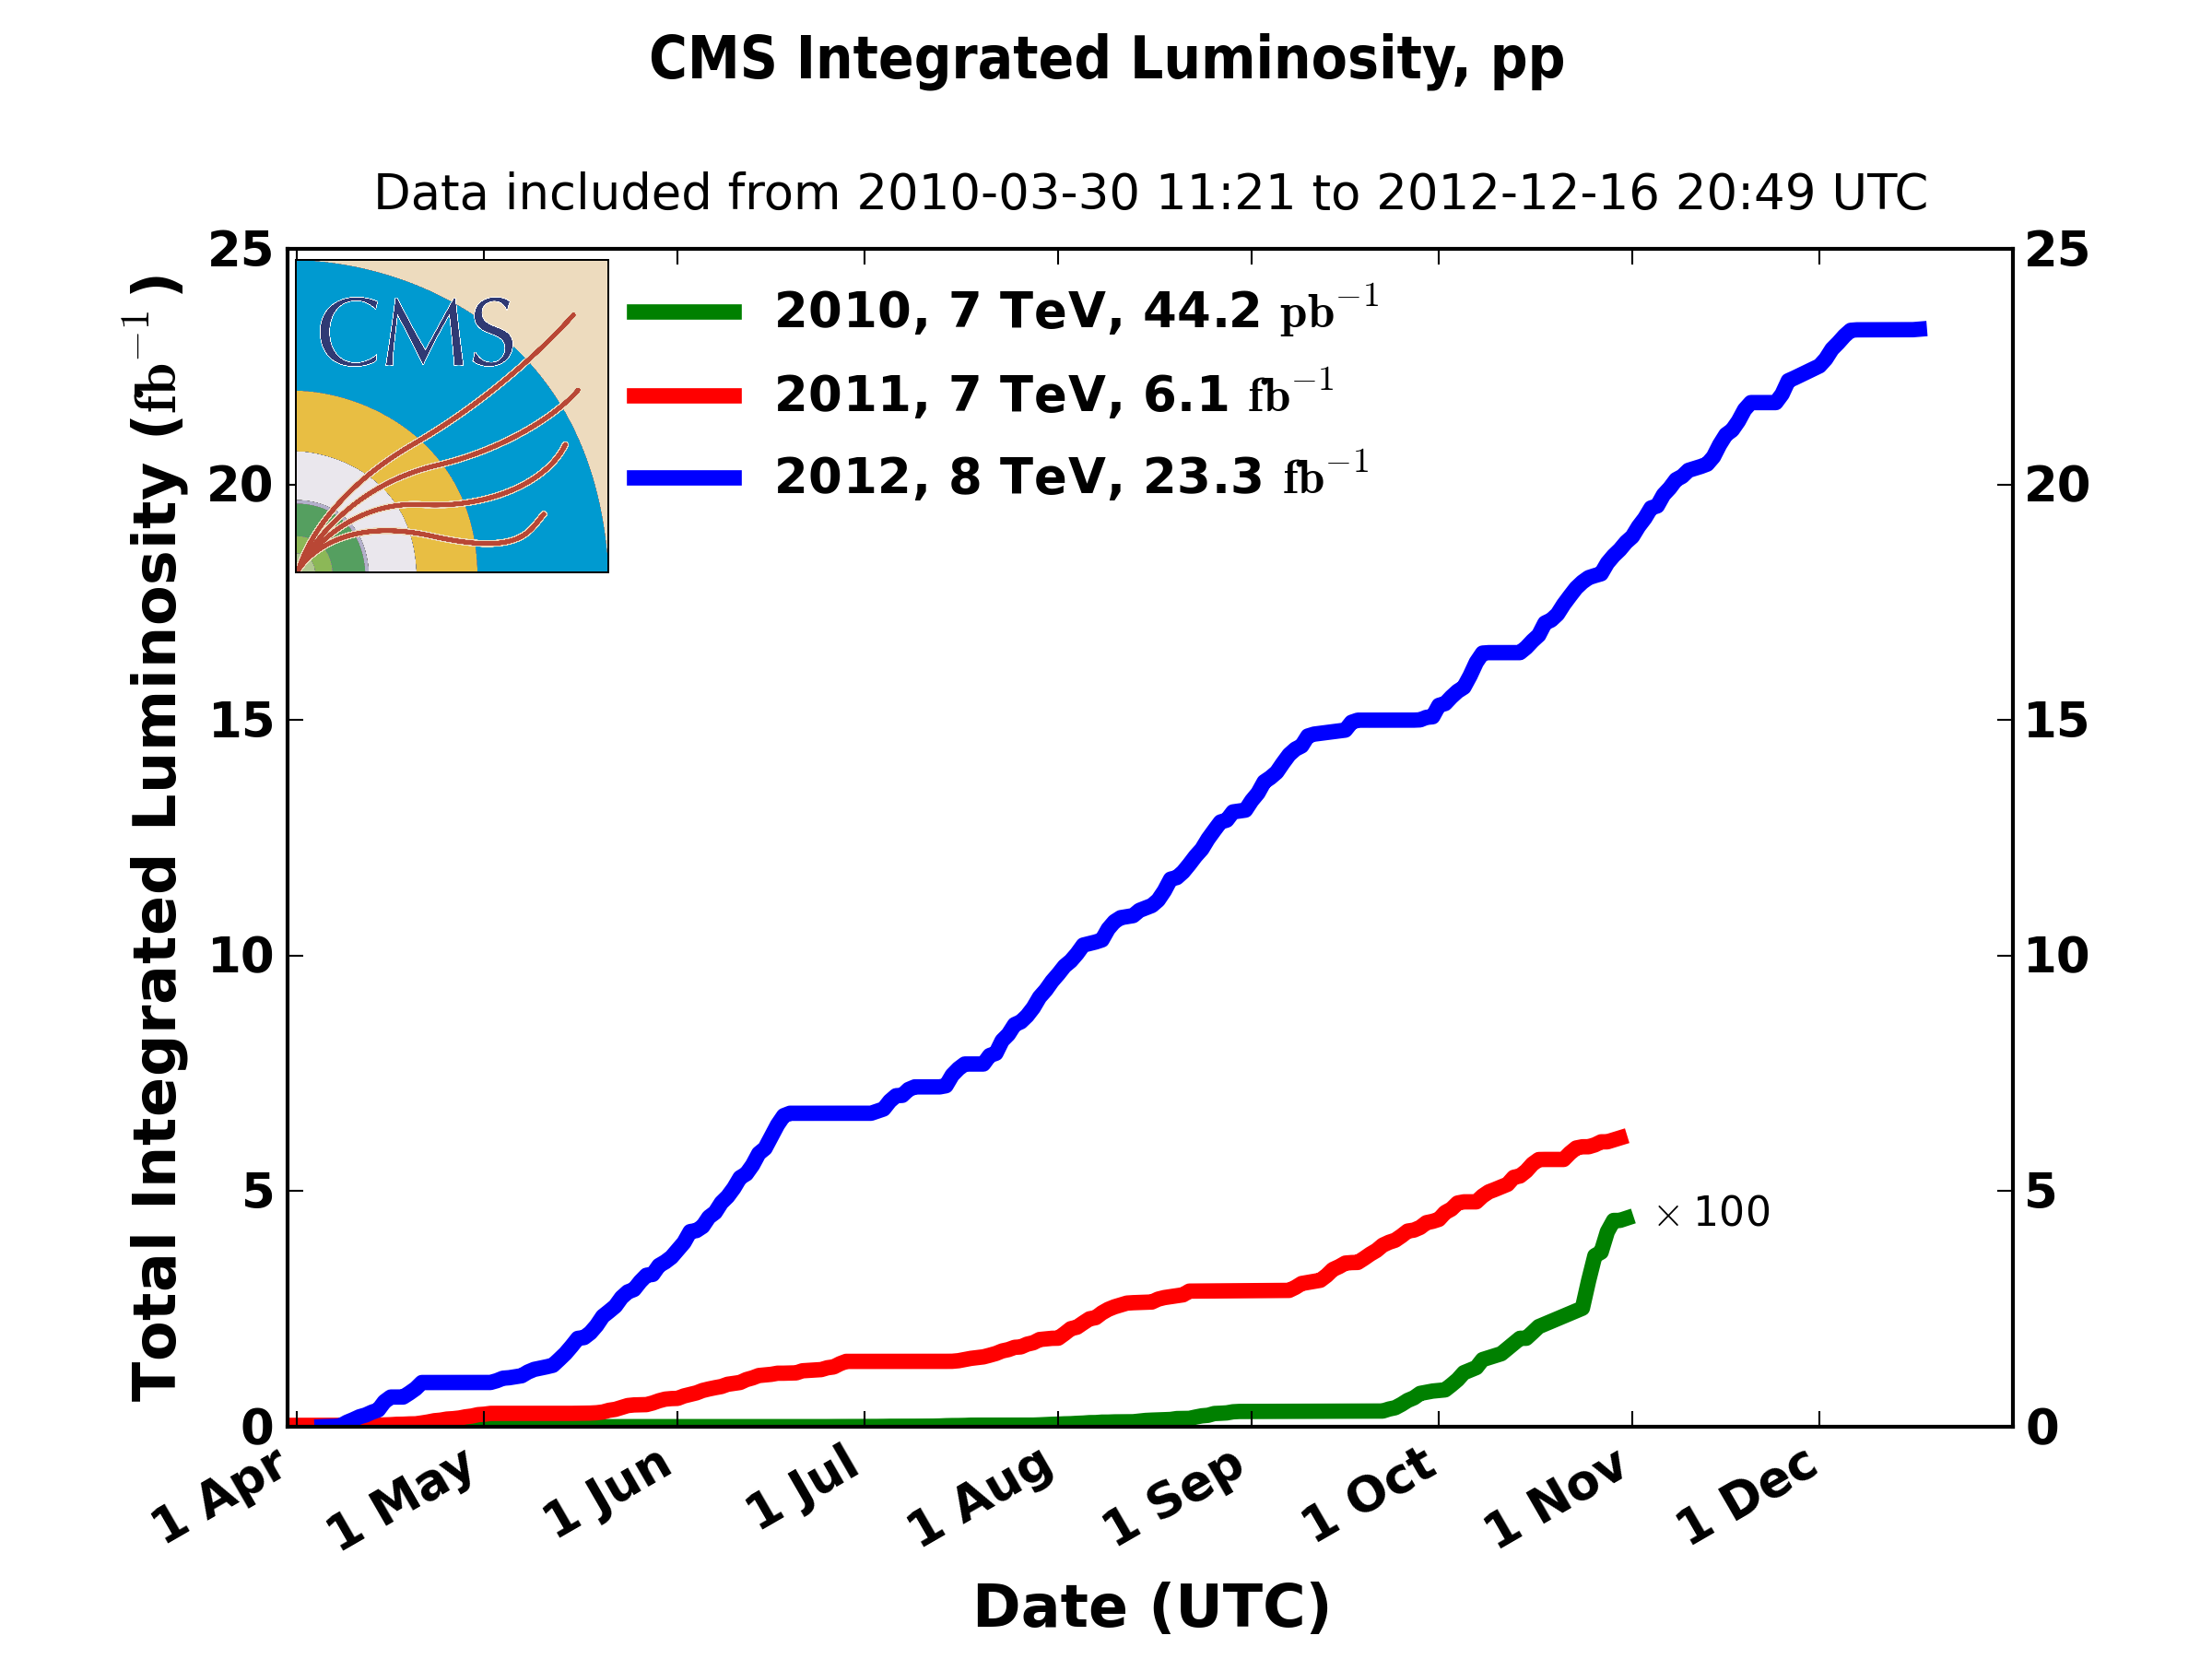
\includegraphics[width=0.75\textwidth]{Chapters/04_Detector/Images/int_lumi_cumulative_pp_2.png}\\
     \caption[Cumulative luminosity delivered to CMS during 2010, 2011 and 2012.]{Cumulative luminosity
     delivered to CMS over time during 2010, 2011 and 2012 proton-proton data taking periods.}
     \label{fig:integrated_luminosity}
\end{figure}

\section{Overview of CMS}
\label{s:Overview}
Compact Muon Solenoid is both the name of the detector at the LHC, and of the collaboration of people
worldwide who work to build, operate, maintain and upgrade it, and to analyse the data it records.

CMS is a general-purpose detector, designed to be efficient at detecting new physics with a wide range of
signals. The detector measures 14.6\m in diameter and 21.6\m in length, and weighs 12500~tonnes
\cite{CMS_experiment}. The different sub-detectors of CMS are arranged in concentric layers around the point
of the beampipe at which the two beams of proton bunches collide, known as the interaction point (see
Figure~\ref{fig:CMS_diagram}). As the products of any collisions that occur in the bunch crossing travel
outwards from the interaction point, they pass through the sub-detectors depositing energy, resulting in
signals being produced. A subset of the information from some sub-detectors (the calorimeters and muon
chambers, described in Section~\ref{s:Subdetectors}) is then processed by a trigger while information from
other sub-detectors is buffered on the detector.

\begin{figure}[hbtp]
   \centering
     \includegraphics[width=\textwidth]{Chapters/04_Detector/Images/cms_120918_02.pdf}\hfill
     \caption[Diagrammatic sectional view of the CMS detector.]{Diagrammatic sectional view of the CMS
     detector
     \cite{Sakuma_sketchup}.}
     \label{fig:CMS_diagram}
 \end{figure}

The design of CMS is based firstly around a superconducting solenoid magnet. Around and inside the magnet are
the sub-detectors: the pixel and strip tracker, the electromagnetic calorimeter, the hadronic calorimeter, the
return yoke for the magnet and the muon detectors. The coordinate system of the detector is designated with
the origin as the intersection point of the two beams in the beampipe, the x-axis positive towards the centre
of the LHC ring, the y-axis positive vertically upwards and the z-axis pointing along the beampipe in an
anticlockwise direction. The azimuthal angle, $\phi$, is defined as the angle in the x-y plane, transverse to
the beampipe starting from the x-axis. The polar angle, $\theta$, is defined as the angle in the z-y plane
starting from the z-axis (the beampipe). The angle $\theta$ is related to the pseudorapidity, $\eta$, by the
formula $\eta=-\ln(\tan(\theta/2))$, so that $\eta$ ranges from 0 at $\theta=90~\degree$ to $\infty$ at
$\theta=0~\degree$~\cite{CMS_TDR1}. The two ends of the detector, at high $\abseta$ values, are called
the endcap regions while the central area at lower $\abseta$ values is called the barrel region. The detector
volume is often denoted in terms of $\Delta R$, with the separation between two particles 1 and 2 being
defined as
\begin{equation}
\Delta R = \sqrt{(\eta_{1} - \eta_{2})^{2} + (\phi_{1} - \phi_{2})^{2}}.
\end{equation}

\section{Sub-Detectors}
\label{s:Subdetectors}

\subsection{Tracker}
\label{ss:Tracker}

The trajectories and charges of particles created in the proton-proton collisions need to be recorded for
later use in particle reconstruction. This is achieved using the tracker section of CMS which consists of
silicon sensors in two forms: pixels and strips. The purpose of the tracker within the CMS detector is to
track the trajectory of charged particles as they travel out from the interaction point. An important
requirement of the tracker is that material budget must be low in order to allow charged particles to pass
through the tracker to outer sub-detectors while minimising multiple scattering, bremsstrahlung radiation,
nuclear interactions and photon conversions. The tracker readout chips must also be capable of distinguishing
in which bunch crossing a particle was produced (bunch-crossing identification), in order for the trigger to
remove particles from previous bunch crossings (termed out-of-time pileup) and fully reconstruct events.

The tracker is split into two parts, with an inner silicon pixel detector and an outer silicon strip detector.
A diagrammatic view of the tracker, including both pixels and strips, is shown in
Figure~\ref{fig:CMS_strip_tracker}. The inner pixel detector consists of three layers in the barrel region at
distances of 4.4\cm, 7.3\cm and 10.2\cm from the beam line with two endcap discs at each end. Each pixel
measures 100\um by 150\um. The entire pixel detector covers an area of only approximately $1\m^{2}$ and
contains 66~million pixels in total.

The strip tracker is comprised of ten layers in the barrel region at distances ranging from 20\cm to 1.1\m
from the beampipe. The four inner layers (at distances of 26\cm, 34\cm, 42\cm and 50\cm from the beampipe)
are collectively named the Tracker Inner Barrel (TIB), while the outer six layers (at distances of 61\cm,
70\cm, 78\cm, 87\cm, 97\cm and 108\cm from the beampipe) are known as the Tracker Outer Barrel (TOB).
The endcaps consist of twelve discs, three of which correspond to the Tracker Inner Discs (TID) at z-distances
from 75\cm to 100\cm, and nine to the Tracker End Caps (TEC) at z-distances between 120\cm and 280\cm
\cite{Palmonari:1260970}. The largest silicon detector ever constructed, the strip tracker contains about ten
million channels and covers an area of approximately $200\m^{2}$~\cite{CMS_experiment,CMS_TDR1}. The operating
temperature of the tracker during 2011 and 2012 was $7.4~\degreeCelsius$ and $0~\degreeCelsius$
respectively for the pixels, and $+4~\degreeCelsius$ throughout for the strips~\cite{Karancsi:2014ofa,
Butz:1497745}.

\begin{figure}[hbtp]
   \centering
     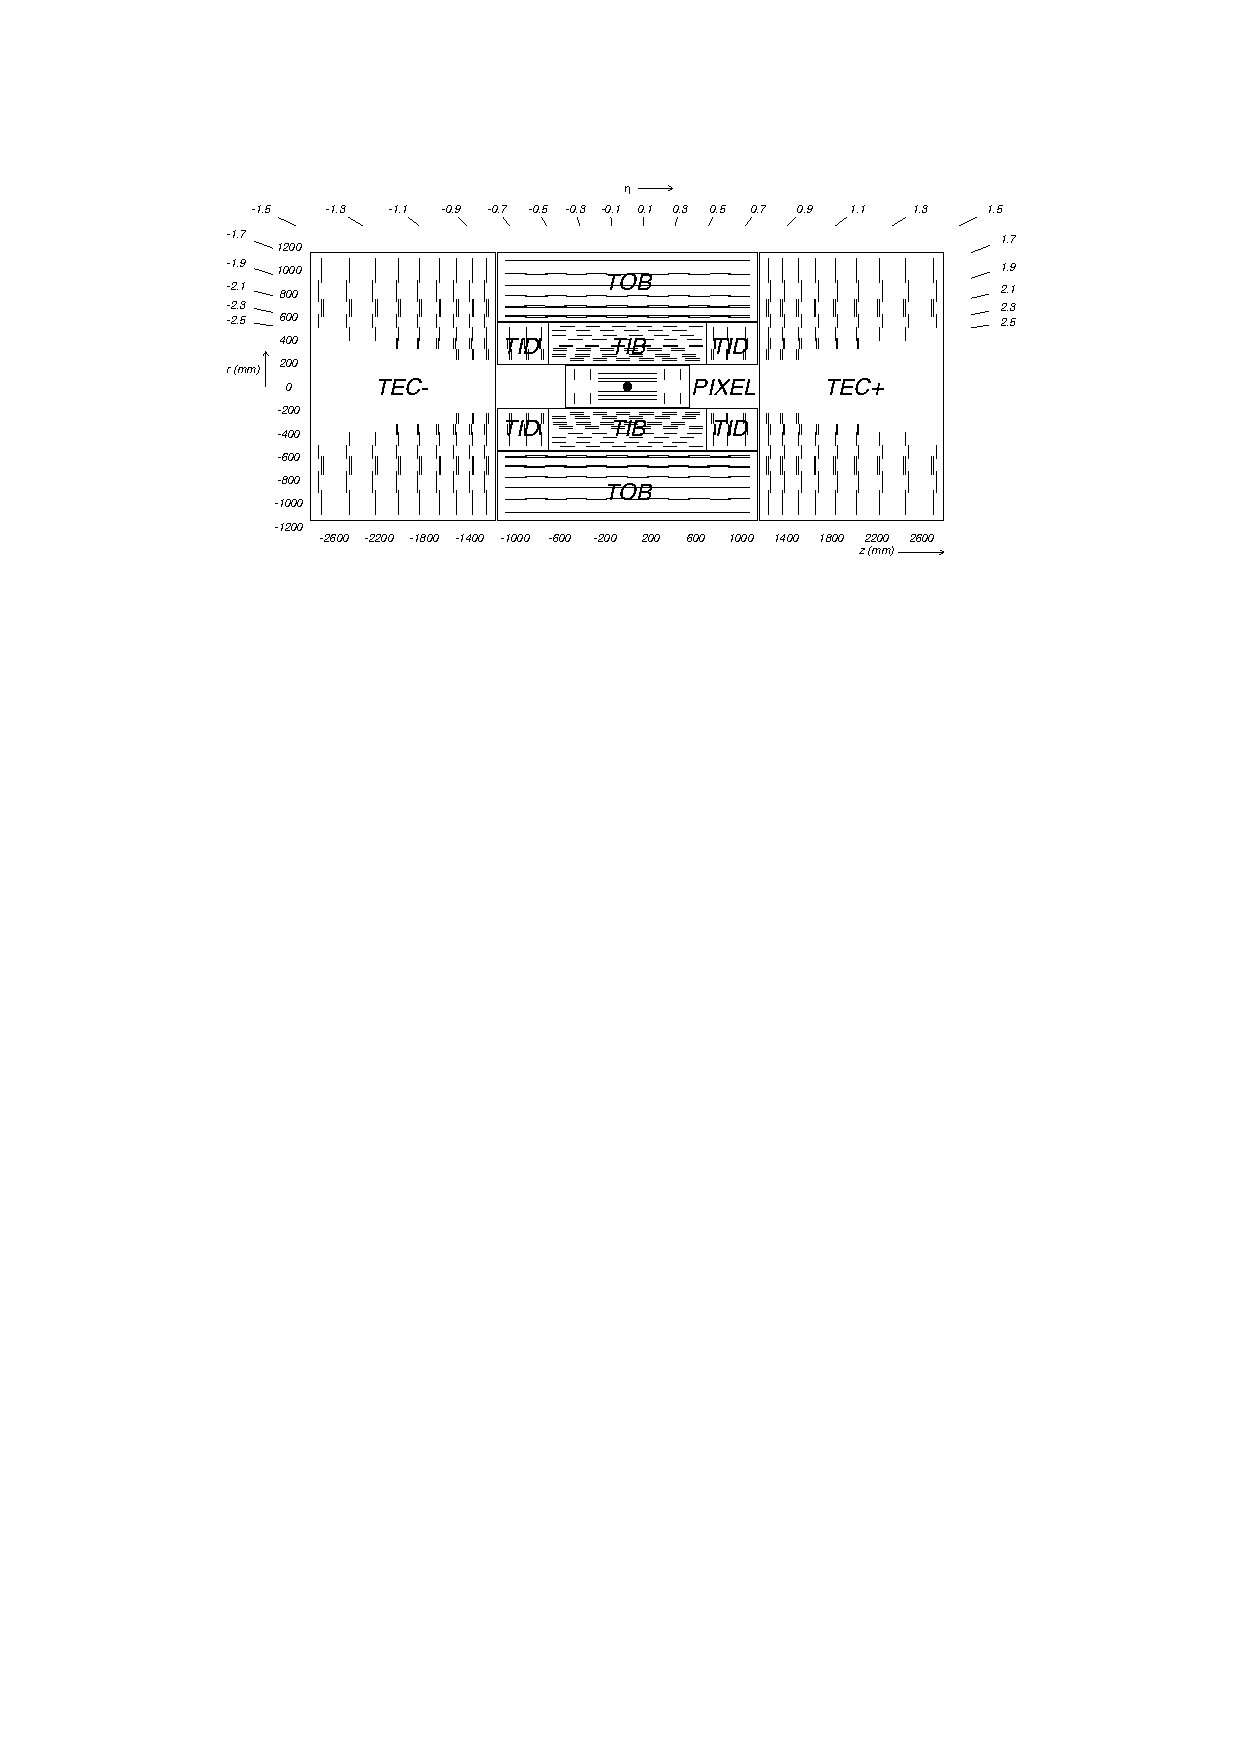
\includegraphics[width=\textwidth]{Chapters/04_Detector/Images/tracker.pdf}\hfill
     \caption[Cross sectional diagram of the CMS strip tracker.]{Cross sectional diagram of the CMS strip
     tracker; each line represents a detector module~\cite{CMS_TDR1}.}
     \label{fig:CMS_strip_tracker}
\end{figure}

As charged particles travel through these silicon sensors, electron-hole pairs are produced that induce a
current in the sensors and are processed by readout chips. This readout is carried out by the Analogue
Pipeline Voltage 25 (APV25) chip. Offline algorithms then use the data relating to which strips and sensors
received `hits' to reconstruct the tracks of charged particles and this information is later used for particle
reconstruction and identification \cite{CMS_experiment,CMS_Tracking_Early_Results}. The curving of particle
tracks within a magnetic field also allows the calculation of the particle momentum and charge, $mv=RqB$,
where $mv$ is the momentum of the particle, $R$ is the radius of curvature, $q$ is the electric charge, and
$B$ is the magnetic field strength.

% Neutral particles could also leave signals in the tracker in a small proportion of cases if the particle
% interacts with a silicon atom and/or converts to charged particles such as a photon conversion to two
% electrons. In the majority of cases, the presence of neutral particles must be detected from their energy
% deposits in the calorimeters.


%With the higher data rate expected after the LHC upgrades over the coming decade,
%pile-up will become an important issue, with approximately 20 interactions per bunch crossing even at the
%current design luminosity. This number is expected to increase to 100-200 following Long Shutdown 3.

%At higher luminosities, the occupancy (the fraction of channels with a 'hit') increases,
%which makes pattern recognition more difficult for track reconstruction algorithms and readout systems. The
%higher tracker resolution desirable for such circumstances also requires more sensors and readout chips. As a
%result, any new chip would need to be more efficient in its use of power whilst processing the data and/or
%require the associated cooling systems to be more efficient. Indeed, studies have shown that the present
%tracker could itself produce acceptable tracking performance in such conditions based on simulations of
%heavy-ion collisions, which produce similar numbers of tracks per event to that expected after the luminosity
%upgrades at the LHC [10].

%The LHC upgrades are split into 2 phases. The pixel detector will be upgraded during Phase 1, and will be an
%on-going process during both Long Shutdown 1, Long Shutdown 2 and shorter intermediate shutdowns. The strip
%detector will be upgraded during Phase 2, more specifically during Long Shutdown 3 [11][12].

The required tracker characteristics of high granularity and high resolution, fast response to process the
high data rate without losing potentially valuable information, radiation hardness and keeping detector
material to a minimum to minimise scattering without minimising the signal, resulted in silicon being chosen
to construct the tracker.

One of the advantages of using silicon over gaseous detectors is that silicon produces more charge carriers
per unit of length travelled by a particle. The silicon sensors that make up the strip tracker in the CMS
detector vary in thickness depending on their location. Sensors of 320\um thickness are utilised in the TIB
and TID, 500\um in the TOB, and a mixture of both thicknesses is used in the TEC. Thicker sensors are used in
the outer sections of the strip tracker in order to maintain a high signal to noise ratio, since the increased
strip lengths in this region lead to increased electronics noise due to higher
capacitance~\cite{CMS_experiment}.

Silicon also allows fast signal transfer, of the order of about 10\ns, as the charge carriers travel quickly
through silicon. Furthermore, the spacing between strips in a silicon sensor, known as the strip pitch, can be
manufactured to be extremely fine (<20\um). The strip pitches in the CMS strip tracker sensors vary from 80\um
to 205\um, and there are fifteen distinct pitch-length
geometries~\cite{Commissioning_and_Performance_Strip_Tracker}.

A further tracker requirement is low occupancy (the fraction of channels with a hit in an event was desired to
be 1~\% or lower at the nominal LHC luminosity) so that pattern recognition can be carried out efficiently and
so that data to be read out is manageable. In order to help maintain such a low occupancy at the nominal LHC
luminosity, the strip tracker has a high granularity, with strip lengths less than 20\cm and strip pitches
less than 205\um~\cite{Palmonari:1260970}. While high granularity is beneficial for high precision tracking,
it also results in a high number of channels, which in turn requires a large amount of electronics for readout
and leads to a high heat load.

On a global scale, the tracker data is read out using a combination of interoperating systems.
The data from the APV25 tracker readout chips is taken via optical fibres to 440 off-detector Front End
Drivers (FEDs) (tracker FEDs make up 63~\% of the total number of FEDs in CMS).
The FEDs then forward the data to the online Data Acquisition System (DAQ). In addition, off-detector Front
End Controllers (FECs) control the front-end electronics by means of approximately 350 control rings,
including triggers, clock and monitoring~\cite{CMS_experiment, Corrin}.

%As a result of the higher collision rates to be expected after
%these upgrades, the CMS tracker will require an improvement in its infrastructure because of radiation damage
%it will have suffered by that point and to ensure that it is robust enough to handle the higher levels of
%radiation after the upgrades. The pile-up is also expected to be in the range of 100 to 200 interactions per
%bunch crossing which also necessitates an improvement in the CMS tracker performance in order to ensure
%valuable data are not lost during collisions \cite{CMS_Silicon_Tracker_upgrade_for_HL-LHC}.

% Within the lattice of pure silicon, there are well-defined bands of energy levels called the conduction band
% and the valence band. The band gap is the difference in energy between these two bands and varies depending on
% the material. At absolute zero, -273$^{\circ}$C, almost all the electrons can be said to be fixed in place in
% this lattice in the valence band, meaning that if an electric field is applied across the silicon, no current
% would be able to flow. When energy is input to the system and an electron gains energy, it may be able to
% cross the band gap to the conduction band, in which case a hole would be present in its previous place in the
% valence band. At this point, both the electron and the hole are mobile and can move freely in current flow,
% for example, under the influence of an electric potential. Materials with a large band gap are insulators, and
% those with a small band gap (or even sometimes with energy bands that overlap with each other) are conductors.
% Silicon, being a semiconductor, has a 'medium' sized band gap of approximately 1.12eV. Nevertheless, the
% number of mobile electrons, above absolute zero, is still large enough to make it difficult to distinguish the
% real signal from the inherent noise in the silicon, known as leakage current (explained in Section 2.3.2).
% In order to decrease this number of free electrons and holes in silicon to obtain a much cleaner signal from a
% traversing particle (i.e. improve the signal to noise ratio), a process called doping is employed to increase
% the number of charge carriers. This involves the substituting of silicon atoms in the lattice with atoms of
% other elements like arsenic, phosphorous, boron or aluminium. In the case of the former two, both have five
% valence electrons. Four of these electrons bond to the four valence electrons present in a silicon atom,
% leaving one electron that can be easily removed from the lattice to the conduction band. This 'donation' of
% electrons to the conduction band increases the number of charge carriers. This type of silicon is called
% n-type silicon because the additional charge carriers are negative. Similarly, if boron or aluminium atoms are
% introduced to the silicon lattice, their three valence electrons bond to the electrons in a silicon atom but
% one silicon electron has nothing to bond to, creating a mobile positive hole. The addition of holes (which
% 'accept' electrons) leads to this type of silicon being called p-type because the additional charge carriers
% are positive.
% Although both p- and n-type silicon increase the number of free charge carriers, a PN-junction can be created
% by attaching a piece of n-type silicon to a piece of p-type silicon. Considering a PN-junction in isolation,
% mobile electrons from the n-type silicon would diffuse into the p-type silicon and unite with the holes from
% the p-type material, leaving behind the positively charged donor atoms. Similarly, the mobile holes from the
% p-type silicon would diffuse to the n-type silicon and leave behind negatively charged acceptor atoms. As
% these electrons and holes move to the two sides of the junction, the resulting electric field opposes the
% initial diffusion of electrons and holes, eventually reaching a state of equilibrium. Once equilibrium is
% reached, this area around the PN-junction will contain no mobile charge carriers and is called the depletion
% region.
% However, if a reverse bias voltage is applied to the silicon (a negative terminal connected to the p-type
% silicon and a positive terminal to the n-type silicon), then the electrons from the n-type silicon, rather
% than diffusing towards the junction, will be attracted towards the positive terminal. Similarly, the holes
% from the p-type silicon will be attracted towards the negative terminal, as shown in Figure 7.
% 
%  
% A higher reverse bias voltage leads to a larger depletion width as more electrons and holes are carried away
% from the junction. At high enough voltages, the width of the depletion region can be made equal to the width
% of the silicon; this voltage is known as the depletion voltage. At this stage, there are no free charge
% carriers anywhere in the silicon and it is in this state that silicon detectors are operated, thus ensuring
% that any charge carriers are only produced as a charged particle travels through the silicon. In this state,
% silicon detectors are effectively reverse biased diodes, only allowing a current to flow in one direction.
 
%Figure 8 - Basic diagram of silicon strip detector with p+ strips (green) on n-bulk (blue) [24].

% The silicon sensors in the CMS strip tracker are p+ strips (which denotes a high concentration of p-type
% impurities) on n-bulk sensors, similar to the diagram in Figure 8. As the silicon is ionised by a traversing
% particle, mobile charge carriers are created which then travel, due to the depletion voltage, to the p+ strips
% (holes) or to the backplane (electrons). As the signal will be created on a particular strip (or strips), it
% will then be possible to deduce the position of the particle.

% 2.3.2 Radiation Hardness The current tracker front-end electronics were initially designed to last about 10
% years in operation under the radiation conditions of the detector [5]. The higher radiation they will be
% subjected to as a result of the higher luminosity and higher collision energies at the HL-LHC will clearly
% impose the requirement that all components, including sensors and electronics, should be manufactured to a
% higher standard of radiation hardness. Radiation damage can occur when particles of high enough energy are
% created in the collisions at the centre of CMS that when they pass through the silicon tracker, they collide
% with atoms in the lattice. This damage is done most often by neutrons, in particular low energy neutrons from
% calorimeters and other detector elements, which interact with nuclei in the silicon and move atoms out of
% place. These atoms are knocked out of place into levels where there is usually no atom, known as interstitial
% levels. An energy of around 15eV is necessary for this to happen; generally at energies of 2keV or less only
% isolated displacements occur, whereas for energies between 2 and 12keV, one or more defect clusters will be
% created. The removal of donor atoms in this way leads to a change in the doping concentrations and eventually
% to an increase in the leakage current (current which may flow when there is no ionising particle traversing
% the silicon). A leakage current will in turn require a higher depletion voltage to remove additional electrons
% or holes captured by the electronically active defects.
% The leakage current is temperature dependent and can be mitigated by using low temperatures. The planned
% running temperature of the CMS silicon tracker in the HL-LHC is planned to be lowered from +4$^{\circ}$C to
% the region of -20$^{\circ}$C to -40$^{\circ}$C due to the benefits in terms of radiation damage. To evaluate
% the behaviour of the proposed CBC in these conditions, an environmental chamber was used to carry out tests at
% varying temperatures in this project. If a leakage current is present, this will lead to noise in the system,
% since current will always flow and any signal would sit on top of this noise. If subject to high levels of
% radiation damage, the leakage current increases to levels at which excessive amounts of power are dissipated,
% and the noise in the readout will be too high to read a clean signal.
% 
% 2.3.3 Noise The aforementioned leakage current is a result of the quantised nature of the charge carriers.
% This noise is present even when there is no signal present, and increases as radiation damage increases the
% leakage current.
% Other potential sources of noise include electronic noise caused by thermal fluctuations of the charge
% carriers. This would manifest as noise in the amplifier at the front end of the CBC and would increase
% proportionally with the capacitance of the connected input system [25]. Another contributor to noise in the
% system could be from non-linearity of the analogue to digital converter (ADC) in the CBC that converts the
% incoming analogue pulse to a digital signal [25].
% The dominant source of noise in our test system is likely to have resulted from electronic noise in the
% connected laboratory setup. In practice, the external noise under operational conditions when the CBC is
% connected to the CMS detector should ideally be maintained lower than the noise in the amplifier.


\subsection{Electromagnetic Calorimeter}
\label{ss:Ecal}
The electromagnetic calorimeter (ECAL), is a hermetic, homogeneous sub-detector constructed of scintillating
crystals of lead tungstate ($\mathrm{PbWO_{4}}$), and is the next layer outside the tracker. Any
electromagnetic particles such as electrons or photons are absorbed by the ECAL crystals which then
scintillate emitting a blue-green coloured light. These signals are then collected and converted to electrical
signals by connected photodetectors, and processed by readout electronics.

The signals in the crystals are collected by avalanche photodiodes in the barrel region and vacuum
phototriodes in the endcaps. The numbers of photoelectrons produced is dependent on temperature, with
increasing temperature resulting in a decrease in the number of electrons at a rate of
$-3.8\pm0.4\%/\degreeCelsius$. A cooling system is thus employed which maintains a stable operating
temperature of the ECAL system to within $\pm0.05\degreeCelsius$, with a nominal operating temperature of
$18\degreeCelsius$~\cite{CMS_experiment}. The energy resolution of the ECAL has been shown to follow
$\sigma_{E}/E = 2.8\%/\sqrt{E}\oplus 12\%/E \oplus 0.3\%$ where the three constant terms come from stochastic
fluctations such as photostatistics, electronics noise and temperature stability and calibration uncertainties
\cite{ECAL_calibration_and_resolution_at_7TeV}.

The barrel region of the ECAL consists of 61,200 crystals and extends up to a pseudorapidity $\eta$ of
$\pm1.479$. Each individual barrel crystal is $25.8X_{0}$ thick, where $X_{0}$ is the radiation length (the
mean distance over which a high energy electron loses all but 1/$e$ of its energy through bremsstrahlung
radiation~\cite{Agashe:2014kda}). They have individual cross sectional dimensions of $22\times22\mm^{2}$, and
are tilted with their front-faces directed towards the nominal interaction point, as can be seen in
Figure~\ref{fig:CMS_ECAL}, leading to each crystal covering $0.0174\times0.0174$ in $\eta-\phi$
plane~\cite{CMS:2010zta}. These crystals are divided into 36 groups, called supermodules, with each
supermodule consisting of 4 smaller modules. The endcaps are comprised of 7,324 crystals, cover the range
$1.479\leq\eta\leq3.0$ and are split into two halves known as ``Dees'', each divided into operating segments
of $40\degree$ each. The endcap crystals have slightly larger dimensions, having a thickness of $24.7X_{0}$
and cross sectional dimensions of $28.62\times28.62\mm^{2}$~\cite{CMS_experiment,ECAL_frontend_monitoring}.
Figure~\ref{fig:CMS_ECAL} shows the layout of the ECAL.

The crystals of high density ($8.28~\g/\cm^{3}$), short radiation length ($X_{0}=0.89\cm$), and small
Moli\`{e}re radius (a measure of the transverse dimensions of electromagnetic showers in a
material~\cite{Agashe:2014kda}) of 2.2\cm lead to a compact calorimeter with fast response time (80~\% of the
light is emitted within 25\ns) and high granularity, capable of withstanding the radiation levels within CMS.

\begin{figure}[hbtp]
   \centering
     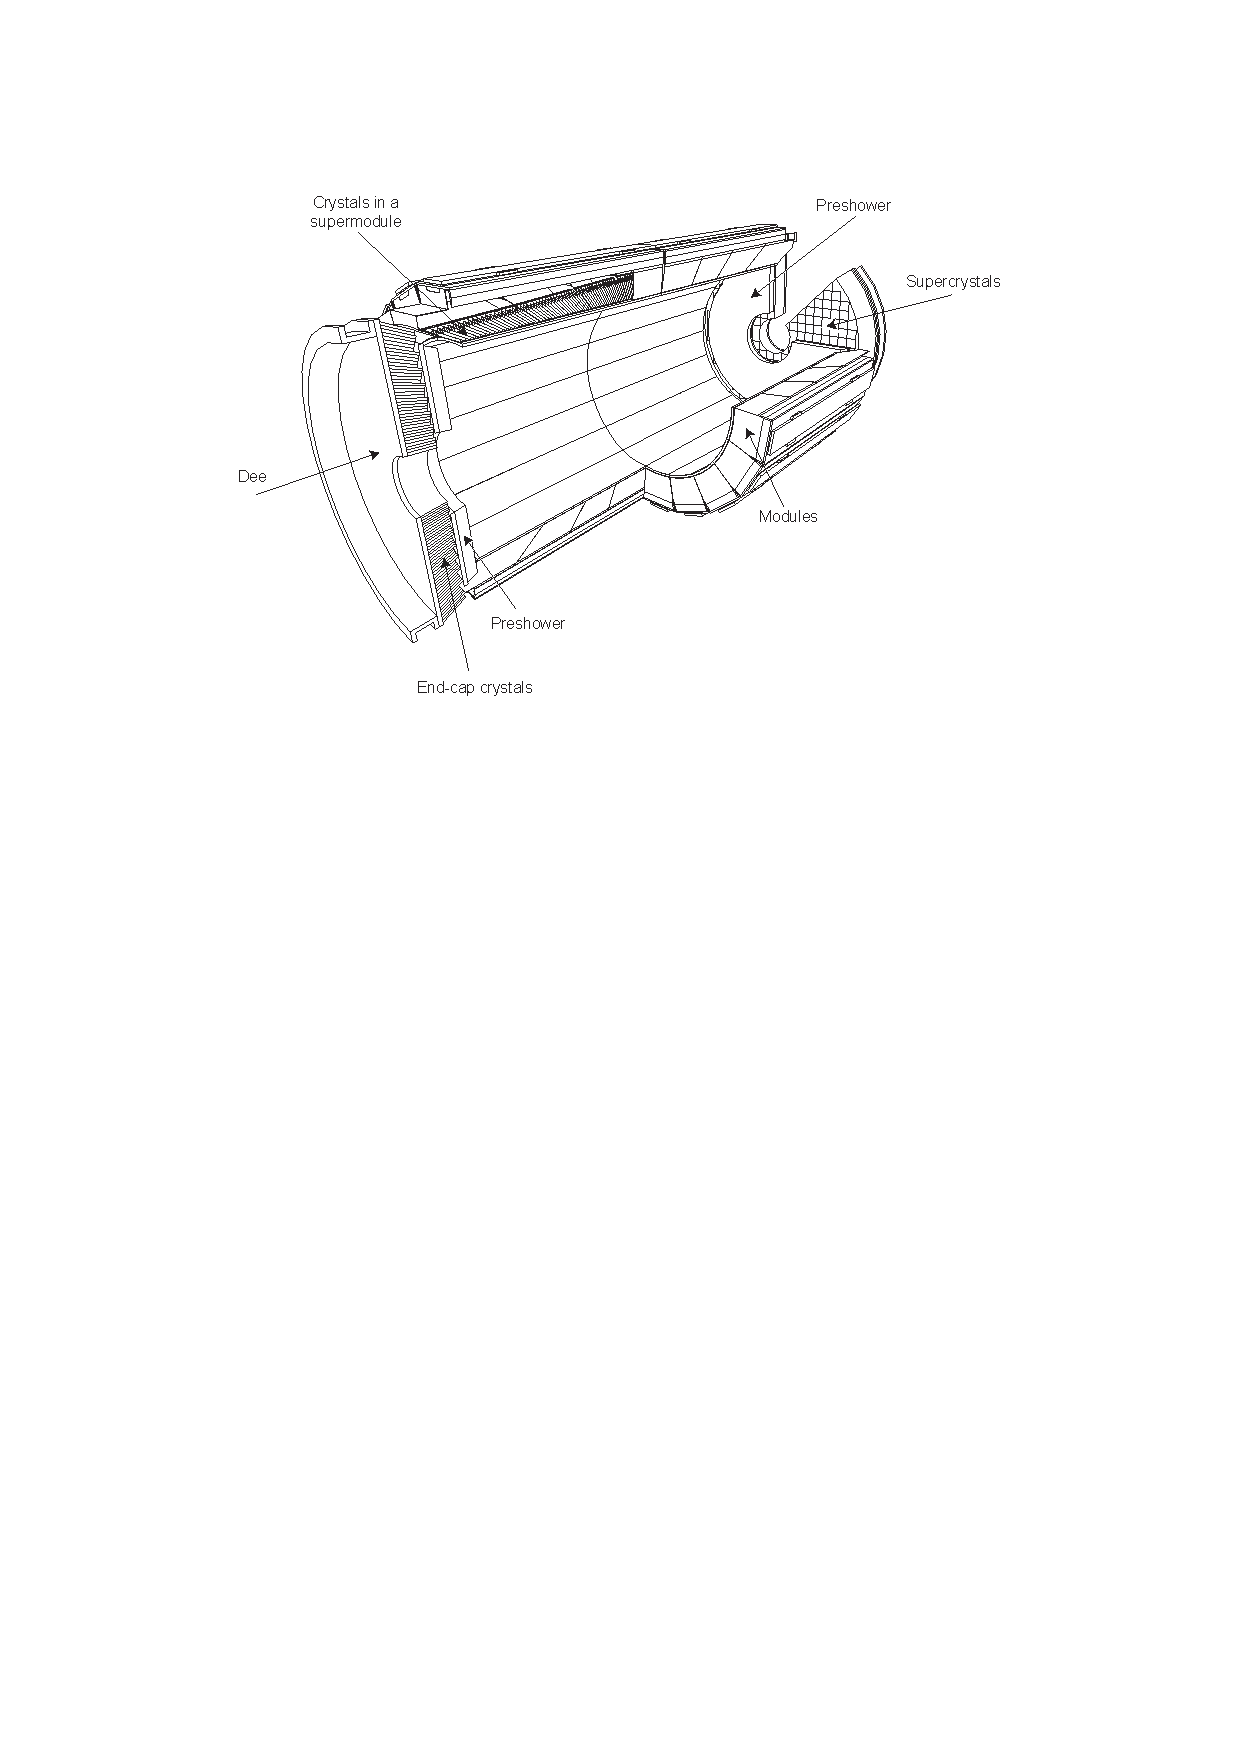
\includegraphics[width=0.7\textwidth]{Chapters/04_Detector/Images/ECAL.pdf}\hfill
     \caption[Diagram of the ECAL showing barrel supermodules, endcaps and preshower detectors.]{Diagram of
     the ECAL showing barrel supermodules, endcaps and preshower
     detectors~\cite{ECAL_calibration_and_resolution_at_7TeV}.}
     \label{fig:CMS_ECAL}
\end{figure}

An ECAL preshower, comprised of two lead plates each followed by a layer of orthogonal silicon strip sensors
(thickness 350\mm, strip pitch 2\mm) is located between the tracker and ECAL endcaps to provide a higher
spatial resolution than the ECAL. This helps to identify, for instance, closely spaced photon pairs
originating from pion decays which may otherwise be identified as a single high-energy photon based on ECAL
energy deposits. As a photon passes through the lead, a shower of electromagnetic particles ($e^{+}e^{-}$
pairs) is produced that are detected by the silicon layers to give a measure of the energy of the photon, while the
orthogonal strips allow a position measurement. The measured energy can then be combined with the energy
measured by the ECAL.

\subsection{Hadronic Calorimeter}
\label{ss:Hcal}
The next sub-detector outside the ECAL is the hadronic calorimeter (HCAL) which works in a similar way to
the ECAL, in this case by absorbing hadron jets. The HCAL is located at a distance of 1.77~m to 2.95~m from
the beamline, with an additional outer hadronic calorimeter also installed outside the magnet due to
radial restrictions imposed by the magnet coil. The HCAL barrel (HB), outer (HO) and endcaps (HE) cover
the $\abseta$ range up to 3.0, with the forward HCAL (HF) placed at $\abseta$ up to 5.2 increasing the
coverage. Figure~\ref{fig:CMS_HCAL} shows a quarter of the HCAL endcap.

The HCAL is a sampling calorimeter, meaning it is composed of alternating absorber layers (made of brass) and
scintillator layers (made of plastic). A hadronic particle produces a shower of secondary particles when it
strikes an absorber layer. The scintillator layers in between the absorbers emit blue-violet light as the
particles traverse them. This process is repeated several times as these secondary particles pass through
successive layers of absorber and scintillator. The light in the scintillators is shifted to the green region
of the spectrum and fed via optical fibres to readout electronics where photodetectors amplify the signal and
the particle energies are measured by summing the measurements over all the layers of the hits in
the HCAL, called a ``tower''.

\begin{figure}[hbtp]
   \centering
     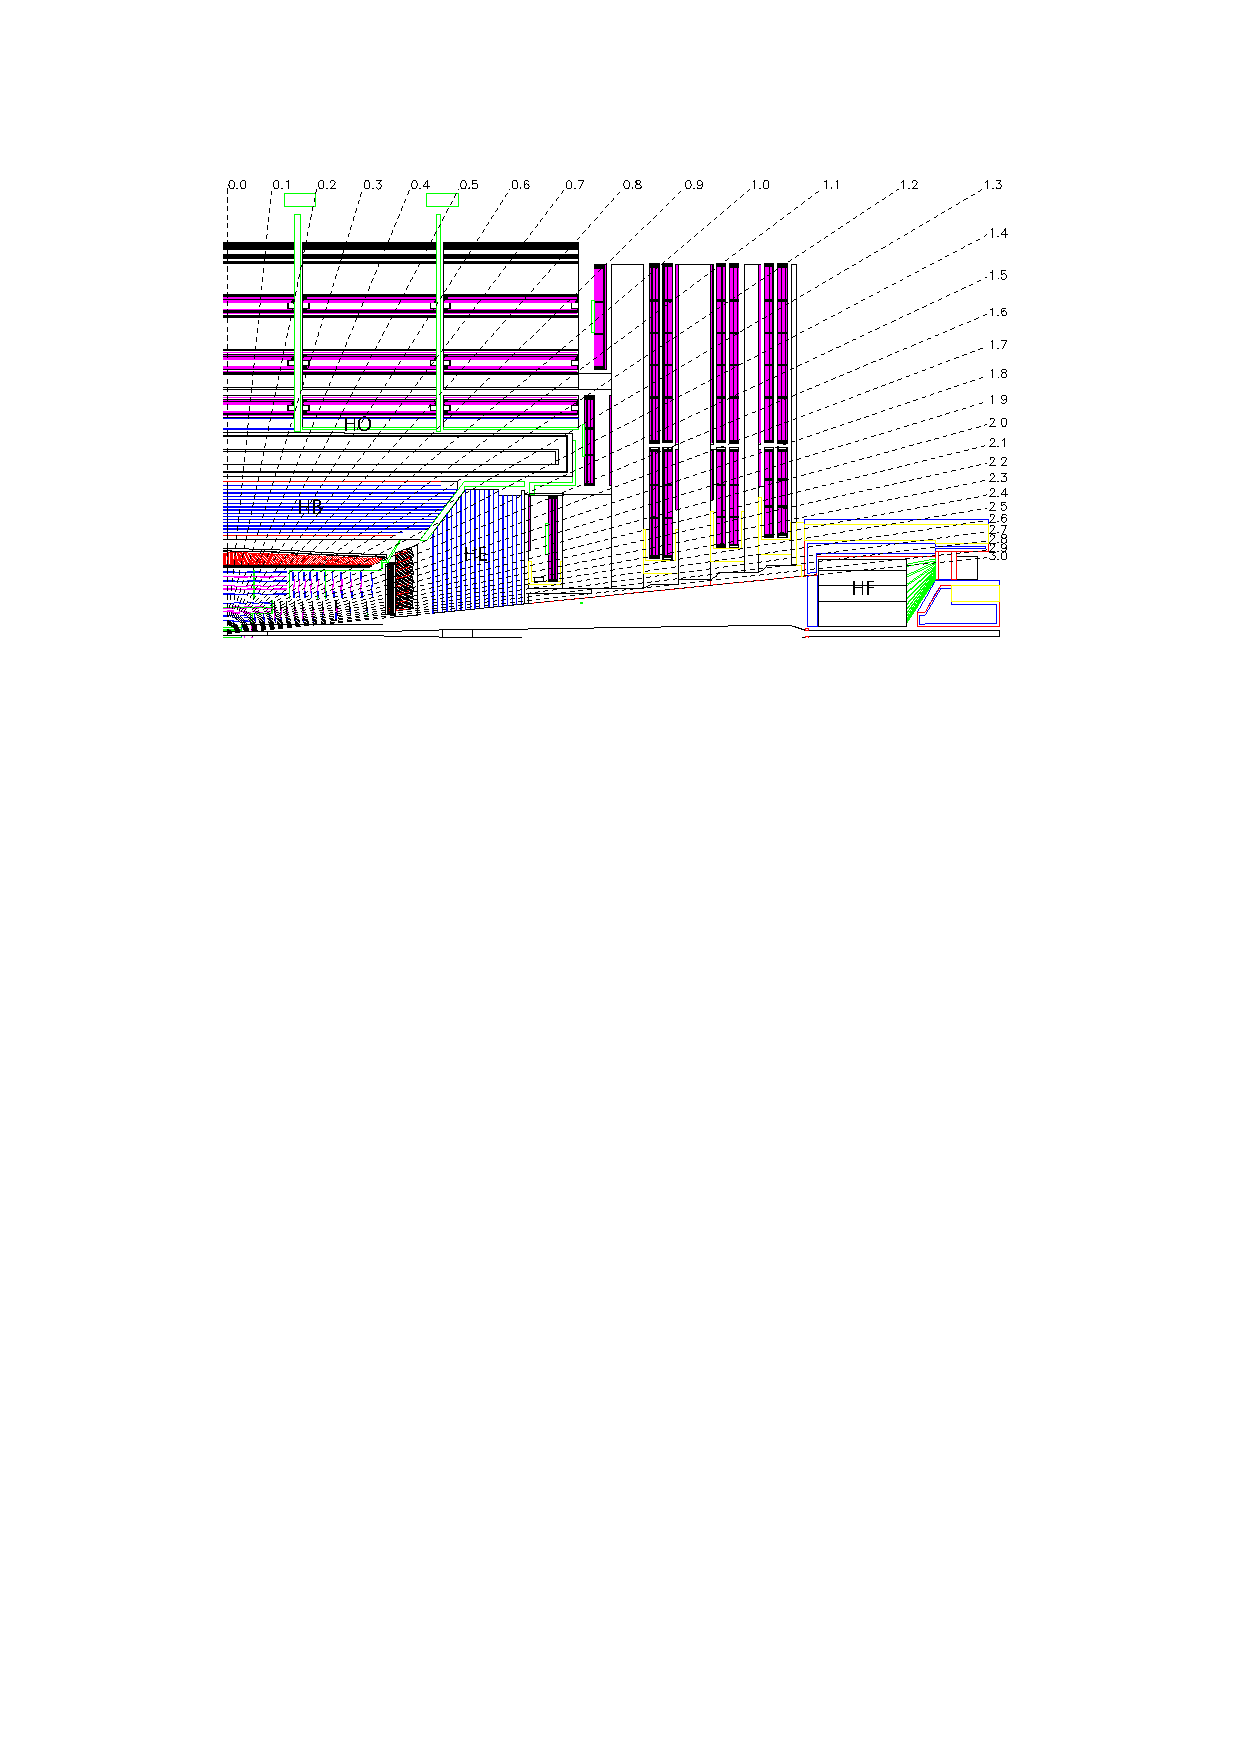
\includegraphics[width=\textwidth]{Chapters/04_Detector/Images/HCAL.pdf}\hfill
     \caption[A longitudinal schematic of the CMS HCAL.]{A longitudinal schematic of the CMS HCAL showing the
     location of the hadron barrel (HB), endcap (HE), outer (HO) and forward (HF) calorimeters
     \cite{CMS_experiment}.}
     \label{fig:CMS_HCAL}
\end{figure} 

\subsection{Superconducting Magnet}
\label{ss:Magnet}
The magnet of the CMS detector is the largest and highest field strength superconducting solenoid constructed
for a physics experiment in terms of bending power for physics and total stored energy~\cite{CMS_experiment}.
It can produce a magnetic field up to 4~\tesla~ (a field strength of 3.8~\tesla~ is used in normal operation)
with a stored energy of 2.7~\giga\joule~\cite{CMS_TDR1}. The cold bore, cooled to 4.5~\kelvin~ using liquid
helium, has dimensions of 12.5\m length and 6\m diameter, and weighs
220~tonnes~\cite{Cryogenic_System_for_Superconducting_Solenoid}.
Due to design constraints and structural requirements, the magnet itself provides some of the structural
strength both to support itself and to withstand its own magnetic bursting force on the coil
\cite{CMS_experiment}.

\begin{figure}[hbtp]
   \centering
     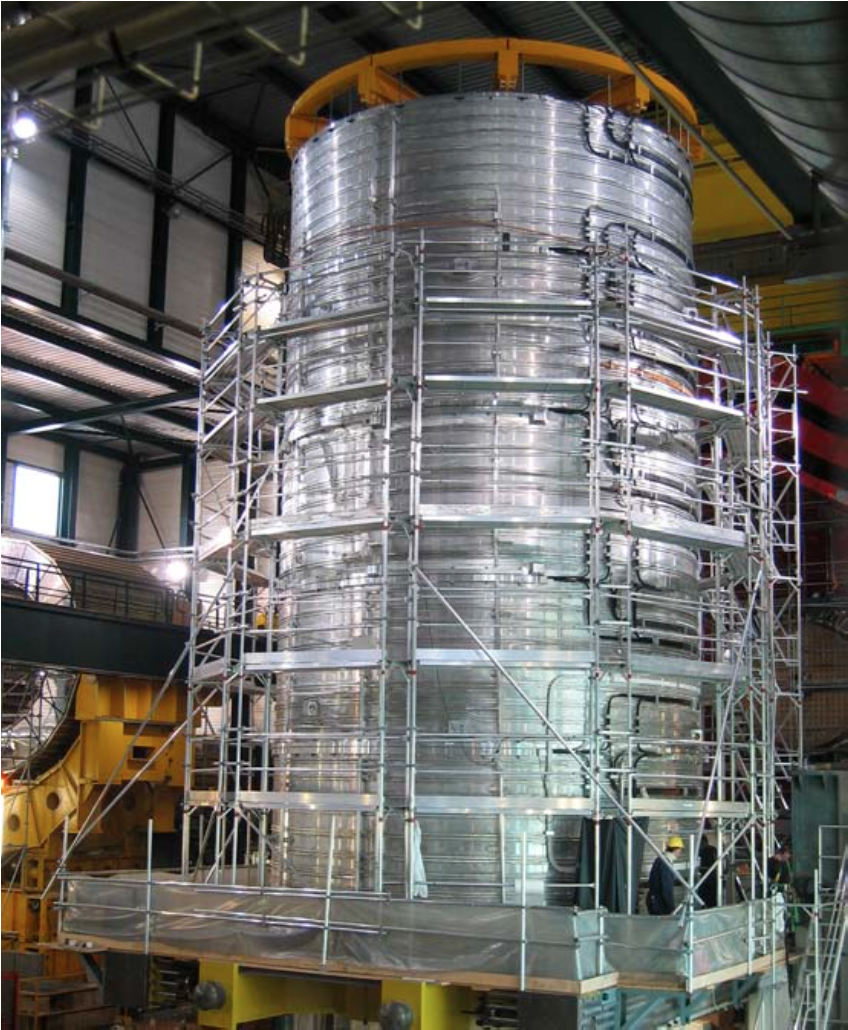
\includegraphics[width=0.5\textwidth]{Chapters/04_Detector/Images/Cold_mass.png}\hfill
     \caption[Bore of the CMS solenoid magnet in vertical position in the CMS assembly hall, SX5.]{Bore of the
     CMS solenoid magnet in vertical position in the CMS assembly hall, SX5, prior to installation \cite{CMS_experiment}}
     \label{fig:CMS_magnet_cold_bore}
\end{figure}
 
The cold bore, pictured in Figure~\ref{fig:CMS_magnet_cold_bore} in the CMS assembly hall, is enclosed in a
steel return yoke weighing 10,000~tonnes with the aim of containing and returning the magnetic field. The yoke
is interspersed with the muon chambers and is made up of 5 barrel segments and 6 endcap discs. The magnet was
designed in a manner such as to facilitate assembly at ground level prior to lowering into the CMS
experimental cavern, UX5. Despite the challenges involved in constructing such a powerful magnet, the high
bending-power created by the high magnetic field was desirable in order to provide good momentum
resolution of the tracking components.

\subsection{Muon Chambers}
\label{ss:Muon_Chambers}
Muons pass through all the previous inner sub-detectors, losing very little energy as they traverse them
(around 1\MeV/\mm on average through the whole detector), leading to the muon chambers being located outermost
in the detector. There are, in fact, three types of muon detectors in use in CMS. The endcaps contain Cathode
Strip Chambers (CSCs), the central barrel regions contain Drift Tubes (DTs), and both regions are equipped
with Resistive Plate Chambers (RPCs). These systems, in combination with the silicon tracker, are used to
determine the momentum of muons by taking advantage of their curved tracks due to the magnetic field. The
different technologies are used due to the different numbers of particles expected in different areas of the
detector and because of technological considerations regarding the physical areas to be
covered~\cite{CMS_TDR1}. Figure~\ref{fig:CMS_muon_system} shows a diagrammatic representation of one quarter
of the CMS muon detectors. The CSCs are used in the endcaps to cover \abseta values between 1.2 and 2.4 that
experience high muon rates and where the magnetic field of the solenoid is high~\cite{CMS_TDR1}. They take the
form of four disc layers each made of 2 (inner layer) or 3 (outer three layers) concentric rings. They consist
of volumes of gas in which positive wires are placed at right angles to negative copper strips. To relate
these to the name given to these detectors, the positive wires are the anodes and the negative strips are the
cathodes. As a charged particle passes through the gas it ionises gas atoms and the electrons that are knocked
out travel towards the anode wires. At the same time the resulting positively charged ions in the gas travel
towards the cathode strips. Since the wires and strips are at right angles to each other, the CSCs provide two
position co-ordinates for the passing muon. The CSC detection mechanism is a fast process so their signals are
used for muon triggering~\cite{CMS_experiment}.
 
\begin{figure}[hbtp]
   \centering
     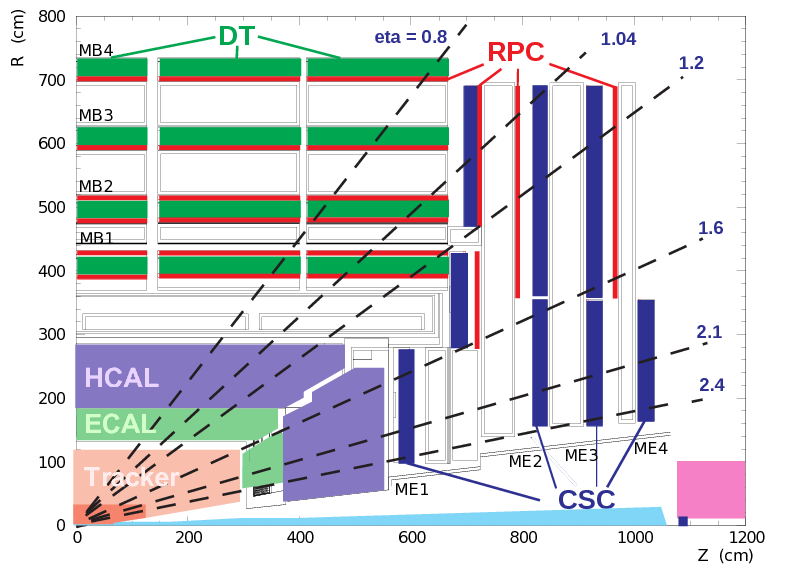
\includegraphics[width=0.65\textwidth]{Chapters/04_Detector/Images/MuonSys-mod3.png}\hfill
     \caption[Schematic representation of a quarter of the CMS muon system.]{Schematic representation of a
     quarter of the CMS muon system \cite{Muon_tracking}}
     \label{fig:CMS_muon_system}
\end{figure}

The barrel region DTs cover \abseta values of less than 1.2, that encounter low rates of low transverse
momentum muons~\cite{CMS_TDR1}. The drift tube chambers are arranged in four cylindrical layers, or stations,
among the layers of the magnet's iron return yoke and RPC layers. The stations are slightly staggered to
ensure that even a muon of high transverse momentum will be detected by at least three of the four layers. The
drift tubes contain a mixture of argon (85~\%) and carbon dioxide (15~\%), and a positively charged stretched
wire. As a particle with a charge traverses the volume of gas, atoms in the gas are ionised and the resulting
free electrons travel along electric field lines towards the positive wire. By using the position of the
electron along the wire and the time taken for the wire to detect the electron, two coordinates of the muon
position can be deduced.
In comparison to the DTs and CSCs, the RPCs that complement them provide a better resolution in terms of time
(1\ns) but a worse resolution in terms of position, and so provide additional trigger information. As their
name suggests, they are constructed of plates, one negatively charged (cathode) and one positively charged
(anode) and made of a plastic with high resistance. In a similar process to the other muon detectors, a gas
that makes up the volume in between the plates is ionised by a passing charged muon. The resulting electrons
create an avalanche of electrons by, in turn, ionising other gas atoms; this avalanche of electrons moves
towards the anode and metal readout strips outside the plastic anode detect the signal for readout. The hit
strips pattern allows a calculation of the muon momentum which is then fed to trigger algorithms.

\subsection{Trigger and Data Acquisition}
\label{ss:Trigger}
At the design bunch crossing frequency of 40~\MHz~ and at the design luminosity of $10^{34}\cm^{-2}\s^{-1}$,
the expected number of proton-proton collisions per second is approximately $10^{9}$, translating to 21
proton-proton collisions per bunch crossing on average. Each bunch crossing produces approximately 1~MB of
data, leading to 40,000\GB/\s~ of data. This extremely large amount of data, which is impractical to record,
means that a trigger system is required to filter the events in order to record only data that are of interest
for physics analyses.

There are two levels to the CMS trigger, named Level 1 Trigger (L1) and High Level Trigger (HLT). These work
with the electronics and readout systems in place in the detector to filter the events to a practically
manageable amount for processing. In combination, these triggers reduce the data rate by at least a factor of
$10^{6}$~\cite{CMS_experiment}.

The L1 Trigger is a pipelined deadtimeless system comprised of calorimeter triggers, muon triggers and a
global trigger that works on a combination of data from the former two. The decisions made by the L1 Trigger
are carried out by custom-designed hardware processors, consisting mostly of programmable electronics such
as Field Programmable Gate Arrays (FPGAs)~\cite{1742-6596-219-3-032009}. The data from a bunch crossing are held in
pipeline buffers in the electronics on the detector (at the front end) whilst the information for the triggers
is processed in the CMS service cavern (USC) and the decisions transmitted back to the front end. The maximum
time allowed for this process for each event is 3.2\us, which is the time taken for the signals to be
transmitted via optical fibres from the detector to the processors, processing time, and transmitted back
again. This time is known as the latency~\cite{CMS_TDR1}. The L1 Trigger outputs events to the HLT at a rate
of 100~\kHz~\cite{CMS_experiment}.

As mentioned, the trigger uses calorimeter and muon chamber data to reach a decision on an event
within the required timeframe. Tracker data are not currently used since track reconstruction exceeds the
amount of time allowed for the L1 trigger decision. Good trigger performance is related to the quality of the
calorimeters and muon systems. Factors such as good momentum resolution of high momentum muons, good charge
determination of muons, good ECAL energy resolution and good missing transverse energy resolution are required
for the trigger to select interesting events. The trigger was designed as described in order to allow the CMS
experiment to meet the goals of the LHC physics programme~\cite{CMS_experiment}.

Unlike the Level 1 Trigger, the High Level Trigger (HLT) is software-based and runs offline in HLT processor
farms of about a thousand commerical processors~\cite{CMS_TDR1}. If the Level 1 produces an accept decision,
the data which was stored in buffers in the front end electronics is read into readout buffers from where the
DAQ system accesses it. The L1 output rate of 100~\kHz~ corresponds to a data rate of approximately 100\GB/\s.
The HLT software processes these events in a computer farm that carries out fast processing of offline
algorithms such as selections and object reconstructions to reduce the rate down to approximately 100~\Hz.
These accepted data are then stored on tape. The HLT algorithms are designed based on the principle of
minimising the number of objects that need to be reconstructed in order to arrive at a decision. Events are
discarded as early as possible, leading to the HLT consisting of many virtual levels that progressively use
more information from, first, the muon chambers and calorimeters, followed by pixel tracker data, and finally
full tracker information~\cite{CMS_TDR1}.

Figure~\ref{fig:single_muon_trigger_rates} shows the variation in trigger rates with increasing muon
transverse momentum at luminosities of $2\times10^{33}\cm^{-2}\s^{-1}$ and $10^{34}\cm^{-2}\s^{-1}$. The rates
for different trigger levels are shown. The L1 trigger rate begins to flatten out as the \pt threshold
increases because the lack of tracker information at L1 means that low momentum muons mis-measured as having
high momentum are not removed. Thus, increasing the threshold would have no discernible effect on reducing the
trigger rates while reducing physics performance by rejecting desirable events. In comparison, the L3 trigger
rate, which includes tracker information, continues to decrease at high muon momenta, and is able to maintain
the rate at the desired level.
% Tracker data could thus be used for improved muon momentum resolution, in addition to electron matching, for
% the application of more efficient isolation criteria, and for primary vertex identification at the L1
% stage~\cite{Klein:1628930}.
% Incorporating the tracker information in the L1 trigger at the HL-LHC would therefore be an effective method
% of maintaining the L1 trigger rate at 100kHz at higher luminosities.

\begin{figure}[hbtp]
   \centering
     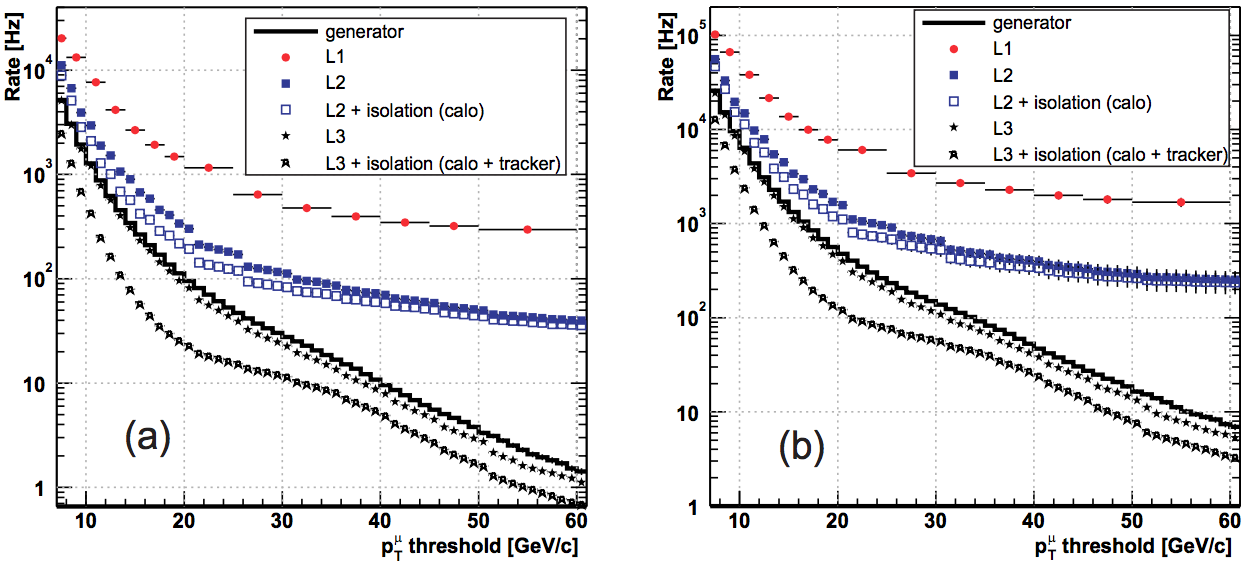
\includegraphics[width=0.65\textwidth]{Chapters/04_Detector/Images/Muon_trigger_rates.png}\hfill
     \caption[Single muon HLT rates at low and high luminosities.]{Single
     muon high level trigger rates at (a) $\mathcal{L}=2\times10^{33}\cm^{-2}\s^{-1}$ and (b)
     $\mathcal{L}=10^{34}\cm^{-2}\s^{-1}$~\cite{Cittolin:578006}.}
     \label{fig:single_muon_trigger_rates}
\end{figure}

A more detailed description of the data acquisition (DAQ) system can be found in \cite{CMS_experiment}
and \cite{CMS_TDR1}.

\section{Upgrades}
\label{s:Upgrades}
The CMS experiment, along with the LHC and the other detectors are in a long term programme of upgrades and
maintenance. By 2023 the luminosity provided by the LHC is expected to be $2\times10^{34}\cm^{-2}\s^{-1}$
\cite{Technical_Proposal_Upgrade_of_CMS_Detector_through_2020}. The various runs and shutdowns until 2023 are
collectively referred to as Phase 1. In phase 2, or after 2023, long shutdown 3 is also planned to bring
further improvements and upgrades to the performance of the LHC, after which the luminosity of the LHC is
expected to reach $5\times10^{34}\cm^{-2}\s^{-1}$. The machine in this state will be known as the high
luminosity LHC, HL-LHC (also sometimes referred to as Super LHC, SLHC).

Naturally, the above dates and schedules are the latest best estimates and are liable to change over time,
particularly those further in the future, as work progresses.
\chapter{CMS Computing and Offline}
\label{c:CMS_computing_and_offline}

\section{CMS Computing}
\label{s:CMS_computing}

The CMS offline computing infrastructure takes on the workload of transferring accepted data from the triggers
to both permanent and temporary storage, of processing this data for subsequent analysis, in addition to the
production of simulated CMS data. The resources needed to process the high volumes of data involved require a
distributed computing system. The Worldwide LHC Computing Grid (WLCG) infrastructure, an international
collaboration of LHC experiments and computing centres, is employed to carry out these tasks.

CMS computing resources are primarily divided into three tiers. Tier 0 (T0) consists of only one site, at CERN
itself. The T0 centre has as its main aim to take accepted data from the detector and transfer it to permanent
storage on tape. Tier 0 computing is also responsible for reconstructing the initial RAW data into smaller
formats, by passing events through modules to produce physics objects (like electrons and jets) using
algorithms to reconstruct tracks in the silicon tracker, clusters of deposits in the calorimeters, primary and
secondary vertices, determine particle identification and to correct for detector characteristics such as
non-functioning components (see Section~\ref{s:Event_Data_Model} onwards for more details on data formats).
From the T0 centre, copies of the data in RECO and RAW format are transferred to T1 centres around the world.
Owing to its crucial role in ensuring the reliable transfer of RAW and RECO data, T0 resources are not
available for analysis by CMS users. There are seven Tier 1 centres located in various countries within the
CMS collaboration. The UK T1 centre is located at the Rutherford Appleton Laboratory in Harwell, near Oxford.
T1 centres provide reliable computing resources for data storage and processing. RAW data is spread between
them, providing a second copy of the RAW data stored at CERN. The second reconstruction step, termed RERECO,
is also carried out at T1 centres, in addition to the production of simulated data. These can then be provided
to any of the Tier 2 centres at CMS institutes (typically universities) where they may be temporarily stored.
T2 centres are also generally used to run users' final analyses and produce simulations
\cite{CMS_experiment,CMS_TDR1}.

\section{Event Data Model}
\label{s:Event_Data_Model}
Reconstructed data from CMS uses a data model based around an event, called the Event Data Model (EDM), where
one event is one crossing of proton bunches at the centre of CMS that passes the triggers. This model
is created and manipulated within a CMS software framework (CMSSW)~\cite{cmssw} written in C++, with the event
and related objects in the object-oriented data analysis framework ROOT~\cite{ROOT}.

The iterations of data from the initial recorded information to subsequent, more compact formats, are produced
by passing events through a sequence of modules. The arrangement of this data takes the form of several
layers, with the first of these being RAW. This level contains the full information from the event in CMS and
occupies approximately 1.5-2~MB/event. More information than is necessary for user analyses is included at
this level, and so the majority of CMS users will not use this data format. Reconstructed level data (RECO) is
slightly smaller in size (approximately 0.5~MB/event) and is essentially a compressed subset of the RAW data
after modules performing reconstruction have been run.

The third level, Analysis Object Data (AOD), is the smallest of the data formats, requiring approximately
100~kB/event, which is small enough to allow the entire AOD data to be stored at computing centres worldwide.
AOD format is a subset of the RECO data, and is produced by further reducing RECO, leaving only high level
physics objects (e.g. electrons, jets) which is adequate for most physics analyses. 

In the differential cross section analysis presented in this thesis, this AOD data is processed using the
Bristol Top Group's NTupleProduction code~\cite{NTT_LukeKreczko_SergeySenkin_JesonJacob_EmyrClement_2015} to
produce private ntuples which are yet again smaller in size, at approximately 3~kB/event. These ntuples are
then converted to simple ROOT histogram files after applying the required selection criteria and corrections
in the BristolAnalysisTools~\cite{BAT_LukeKreczko_JesonJacob_SergeySenkin_EmyrClement_2015}. Scripts written
in Python in DailyPythonScripts~\cite{DPS_LukeKreczko_SergeySenkin_JesonJacob_EmyrClement_2015} are then used
to produce final results plots and tables.

\section{Object Reconstruction and Identification}
\label{s:object_reconstruction_and_identification}

The process of producing a physics object such as an electron, photon or jet, from the data recorded by CMS is
known as reconstruction and is carried out by modules known as EDProducers within CMSSW. The three-step
process of reconstructing high level objects consists of local reconstruction within a sub detector, global
reconstruction using data from the whole CMS detector, and a final stage combining reconstructed objects from
the first two stages. The reconstruction technique used in the majority of CMS analyses is called Particle
Flow (PF) \cite{particle_flow}. The PF algorithm uses information from all of the sub-detectors in CMS to
identify and reconstruct and identify all stable particles produced from a proton-proton collision. There is
no lower threshold applied to PF objects, but this is dependent on the resolution of each of the
sub-detectors.

\subsection{Track Reconstruction}
\label{ss:track_reconstruction}
Algorithms performing local track reconstruction execute a scan to identify tracker modules that receive a
higher than threshold signal. Clusters are then constructed by adding adjacent strips or pixels to the
originally identified seed strip or pixel to provide a measurement of the hit position. In order to
reconstruct complete tracks to obtain the trajectory and momentum of the charged particle, these clusters are
then input to track finding algorithms. These algorithms are based on specific requirements, such as high or
low transverse momentum tracks, and are collectively known in CMS as the Combinatorial Track Finder (CTF).

Multiple passes of the CTF reconstruction software are carried out to reconstruct tracks, in a process called
iterative tracking. The earliest iterations identify tracks that are easy to find such as high \pt tracks
originating near the interaction point. As these tracks are reconstructed, the corresponding hits are removed
from consideration in subsequent iterations, making it simpler for later iterations to identify tracks that
are more difficult to find such as those of displaced particles or with low \pt.

Six iterations are carried out in total, and each iteration can be split into four steps. Seeds are created
using 2 or 3 hits to produce initial track candidates. The seed gives an estimate of the trajectories of the
potential track candidates. A Kalman Filter \cite{kalman_filter, Speer:927395} based track finding algorithm
then looks for further hits along an extrapolated path of the seed trajectory. A track fitter is then run
using information from the previous steps to produce final values for trajectory parameters. The fourth and
final step then rejects tracks which fail specified quality checks \cite{track_reconstruction}.

\subsection{Pileup Subtraction}
\label{ss:pileup_subtraction}
When reconstructing an event in CMS, all vertices (points from which multiple tracks originate) in the event
must be reconstructed. By ordering the vertices by the sum of the transverse momenta of their tracks, it is
possible to identify the vertex of interest for physics analyses, known as the primary vertex (PV), as the
vertex with the largest transverse momentum. The particle flow algorithm reconstructs objects, starting with
those coming from the primary vertex, followed by other vertices (known as pileup). The reconstructed objects
from the PV can be affected by the number of other vertices present in the event. For example, the jet
momentum and lepton isolation could both increase with high pileup. This can, in turn, lead to signal events
not passing selection requirements because a truly isolated lepton from the PV may appear not to be isolated.
In addition, a larger number of events from background processes may pass selection requirements due to low
energy jets appearing to have a higher energy. Hence, pileup subtraction, the removal of charged particles
coming from vertices other than the PV is implemented to reduce these effects.

Neutral particles, however, pose a more difficult problem since they leave no tracker information for the
reconstruction algorithms to easily identify their origin. One method of removing such particles from an
event, known as the $\Delta\beta$ correction, uses the fact that the estimated average energy in an event from
neutral particles from secondary vertices is half that from charged particles from secondary vertices. Thus,
it can be estimated that 0.5 times the charged particle energy comes from neutral particles from secondary
vertices. The corrected energy is calculated by Equation~\ref{eq:delta_beta}, where $\Delta\beta=0$.
\begin{equation}
\label{eq:delta_beta}
E_{\text{corrected}} = E_{\text{charged hadrons from PV}} + max(0, (E_{\text{photons+neutral hadrons}}) -
\Delta\beta \cdot E_{\text{charged hadrons from PU}})
\end{equation}
The second method, known as $\rho$ correction, subtracts an average transverse momentum coming from pileup per
unit area. While the two methods produce similar results, the $\rho$ correction is used to correct the
electron isolation and the $\Delta\beta$ correction is used to correct the muon isolation in the differential
cross sections analysis presented in this thesis, as recommended by the CMS TOP physics analysis group.

\subsection{Electron Reconstruction}
\label{ss:electron_reconstruction}
ECAL local reconstruction algorithms calculate the time of arrival, position and the energy of deposits. After
grouping together deposits in neighbouring crystals to form clusters, deposits are then matched to deposits in
the HCAL, forming a Calo Tower. Electrons are, typically, completely stopped in the ECAL and deposit their
energy in a narrow cluster of crystals.

However, electrons can interact with the material between the interaction point and the ECAL, emitting a
photon via bremsstrahlung radation. Similarly, photons can convert to an elecron-positron pair ($e^{+}e^{-}$).
Both of these processes result in ECAL deposits with a larger spread in $\phi$ because of the strong magnetic
field in the inner section of CMS containing the tracker. In the case of photons, several clusters are grouped
together to form superclusters, which are then corrected for their energies to obtain the energies of the
original photon \cite{photon_reconstruction}.

Electron reconstruction in the ECAL is carried out by two methods. The first matches superclusters with a
trajectory compatible with two or three pixel detector hits and the interaction point. The second matches the
supercluster to tracker tracks to identify electrons (and in the case of electrons emitting bremsstrahlung
radiation, tracks with a low number of hits) \cite{electron_reconstruction}. Combining the seeds from the two
methods, a Gaussian-Sum Filter (GSF), a generalisation of the Kalman Filter (KF) algorithm, is used to
reconstruct electron paths \cite{electrons_GSF}.

Since other objects can leave similar signatures to electrons in the detector, such as jets or electrons from
photon conversions, candidates are required to satisfy additional requirements of identification and
isolation. Several electron identification methods exist and are used in CMS analyses. The top cross sections
analysis in this thesis uses the multivariate identification (MVA ID). As the name suggests, this approach
uses a multivariate analysis to produce a discriminator value, with higher values indicating a higher
likelihood for a candidate to be a real electron. The MVA ID algorithm is optimised for identifying electrons
from \W and \Z boson decays, and separately for triggering and non-triggering
electrons~\cite{electron_reconstruction}. The MVA ID algorithm takes the following track, track quality, and
supercluster variables as input:
\begin{itemize}
  \item The measured bremsstrahlung fraction $f_{brem}$, based on the change in track momentum between the
  vertex and the outermost hit.
  \item The $\chi^{2}_{GSF}$ of the GSF track.
  \item The $\chi^{2}_{KF}$ of the GSF track.
  \item The number of KF track hits.
  \item $\Delta\eta_{vtx}$, the distance in $\eta$ between the supercluster and the track at the vertex.
  \item $\Delta\phi_{vtx}$, the distance in $\phi$ between the supercluster and the track at the vertex.
  \item $\Delta\eta$, the distance in $\eta$ between the supercluster and the extrapolated track.
  \item $\Delta\phi$, the distance in $\phi$ between the supercluster and the extrapolated track.
  \item $\sigma_{i\eta i\eta}$, the cluster shape in $\eta$. 
  \item $\sigma_{i\phi i\phi}$, the cluster shape in $\phi$.
  \item The width in $\eta$ of the supercluster
  \item The width in $\phi$ of the supercluster
  \item $1-\frac{E_{1\times5}}{E_{5\times5}}$, 1 minus the ratio of the energy in the central $1\times5$ strip
  of the $5\times5$ electron cluster, to its total energy. 
  \item $\frac{E_{3\times3}}{E_supercluster(raw)}$, the ratio of the energy in a $3\times3$ electron cluster
  to the raw supercluster energy.
  \item $H/E$, the ratio of the energy in the HCAl to the energy in the ECAL.
  \item $E_{supercluster}/\p$, the ratio of the energy of the supercluster to the momentum of the associated
  track.
  \item $\frac{1}{E_{ECAL}}-\frac{1}{\p}$, the inverse of the ECAL energy minus the inverse of the momentum of
  the associated track.
  \item $\frac{E_{e}}{p_out}$, the ratio of the electron cluster energy to the outer track momentum. 
  \item $\frac{E_{preshower}}{E_{supercluster(raw)}}$, the ratio of the preshower energy to the raw
  supercluster energy.
  \item $\eta$ of the supercluster.
  \item $\pt$ of the associated track.
  \item $d_{xy}$, the transverse impact parameter, and the 3D impact parameter.
\end{itemize}

The isolation of an electron, defined as the activity within a cone surrounding the electron, is used as an
additional criterion to select electrons, in particular to identify electrons promptly produced in a
proton-proton collision. Such isolated electrons would have less activity in their vicinity than electrons
from within a jet, which could originate from leptonically decaying b hadrons, and jets faking electrons. Two
methods exist in CMS of calculating the isolation of a particle: detector based isolation and particle based
isolation. The detector based method is defined in each sub detector as the sum of the momenta or energies in
a cone of $\Delta R = 0.3$ around the electron. The particle based method uses the total transverse energy of
PF reconstructed particles within a cone of $\Delta R = 0.3$ and can remove activity coming from collisions
other than the hard proton-proton interaction of interest. By normalising this isolation to the momentum or
energy of the electron, a relative isolation is obtained, relating the cone activity to the electron. Termed
PFRelIso, this method of calculating relative isolation is used in the cross sections analysis to select
electrons.
% can improve signal efficiency

In order to avoid the selection of electrons originating from a photon conversion, a veto can be placed on a
second electron in the event. However, since the two electrons in a photon conversion may not necessarily have
equal transverse momentum, \ie one may have a very low \pt, such a veto may be insufficient, and so further
techniques to identify conversion events are used. Firstly, since an electron from a conversion would be
produced at some distance from the interaction point and in the detector material, eliminating candidates with
missings hits in the pixel tracker helps to distinguish such electrons from promptly produced electrons. In
events in which the conversion occurs in the beam pipe or if the electron is matched to unassociated pixel
hits, this method can also be insufficient, so an additional track matching step is used. Tracks are matched
in pairs and following geometrical cuts, can be removed if they appear to originate from a conversion
\cite{electron_reconstruction}.

\subsection{Muon Reconstruction}
\label{ss:muon_reconstruction}
Local reconstruction in the muon chambers provides hit position and time of arrival of a muon. This
information from the DTs and CSCs is amalgamated to create muon track hits and segments, which are then used,
together with track candidates from the RPCs, by the muon global reconstruction algorithms to reconstruct
\textit{standalone-muon tracks}~\cite{muon_reconstruction}. An inner detector segment from the muon chambers
is used as a seed for a Kalman Filter~\cite{kalman_filter, Speer:927395} and possible trajectories are generated. By removing hits
which are unlikely to have come from the track in question, the likely trajectory is constructed
layer-by-layer. A final fit is carried out, including an extrapolation to the interaction point for greater
momentum resolution.

Muons are also independently reconstructed in the tracker. These \textit{tracker tracks} can therefore be
combined with the aforementioned muon chamber information, where the magnetic field is only 2~\tesla, to
improve the \pt resolution of muons, as seen in Figure~\ref{fig:muon_momentum_resolution}.

\begin{figure}[hbtp]
   \centering
     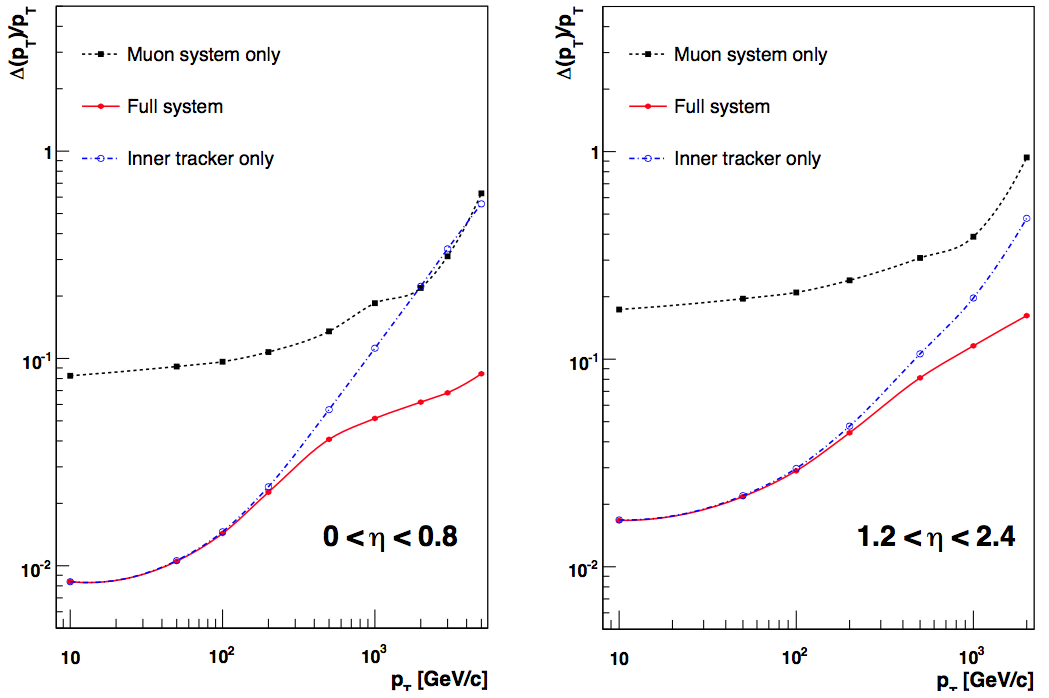
\includegraphics[width=0.65\textwidth]{Chapters/05_Computing_And_Offline/Images/muon_momentum_resolution.png}\hfill
     \caption[Muon transverse momentum resolution using muon system and the tracking system.]{Muon transverse
     momentum resolution as a function of muon transverse momentum using the muon system only, using inner tracking only,
     and using both~\cite{Chatrchyan:2012xdj}.}
     \label{fig:muon_momentum_resolution}
\end{figure}

Two methods are employed to combine the information from the two sub-detectors. \textit{Global muon}
reconstruction matches a \textit{tracker track} to a \textit{standalone-muon track} and carries out a fit of
the resulting \textit{global muon} track. The second method, \textit{tracker muon} reconstruction,
extrapolates tracker tracks above a threshold of \pt$>0.5\GeV$ and \p$>2.5\GeV$, outwards to the muon
chambers. A muon candidate is accepted if a DT or CSC matching track is found and the muon \pt is greater than
0.5\GeV. The \textit{global muon} reconstruction method has a higher efficiency for muons of high \pt while
the \textit{tracker muon} reconstructs low momentum muons ($\leq5\GeV/c$) more
efficiently~\cite{muon_reconstruction}. In the case of the semileptonic differential cross sections analysis
presented in this thesis, since the signal in the muon channel involves a single highly energetic muon, muons
reconstructed using the \textit{global muon} reconstruction method are used.

For triggering, the \pt of a muon is first estimated using the information available at Level 1 from all three
types of muon detectors. At HLT level, the muon candidates from Level 1 are further refined using track
finding and fitting, but still using only information from muon chambers, leading to Level 2 muons. As
mentioned in Section~\ref{ss:Trigger}, due to the time constraints required of the L1 trigger, full tracker
data are not currently used. However, tracks of Level 2 muons are extrapolated into the tracker systems and a
localised track finding algorithm is run to identify only nearby tracker hits. A track matching that of a
Level 2 muon leads to a Level 3 muon.

\subsection{Jet Reconstruction}
\label{ss:jet_reconstruction}
As quarks produced in proton-proton interactions (except the top quark) hadronise~\cite{Griffiths:1987tj},
jets of particles are formed in the general direction of travel of the quark. The time of arrival, position
and the energy deposited by hadronic objects are locally reconstructed in the HCAL. If the deposit matches an
ECAL deposit, a Calo Tower is formed for later use in jet reconstruction algorithms.

The PF algorithm performs the reconstruction of particles, and the \antikt algorithm is used to perform the
clustering of these particles into jets. The \antikt algorithm, explained in detail in~\cite{Cacciari:2008gp},
is one of several jet algorithms that exist in CMS to combine reconstructed particles into jets. It defines a
distance $d_{ij}$ between reconstructed particles as
\begin{equation}
%\begin{center}
d_{ij} =
min\left(\frac{1}{p_{T,i}^{2}},\frac{1}{p_{T,j}^{2}}\right)\frac{(\eta_{i}-\eta_{j})^{2}+(\phi_{i}-\phi_{j})^{2}}{R^{2}}.
%\end{center}
\end{equation}
$p_{T,i}$ and $p_{T,j}$ are the transverse momenta of the two particles $i$ and $j$, $\eta_{i}$ and $\eta_{j}$
are the rapidities, $\phi_{i}$ and $\phi_{j}$ are the azimuth angles and $R$ is the radius of the jet cone.
The \antikt algorithm iteratively clusters together particles with the smallest $d_{i,j}$ between them until
all PF objects in the event have been clustered into jets. Events will usually consist of a small number of
high-\pt (hard) particles and a large number of low-\pt (soft) particles. The distance between hard particles
is typically small, and the distance between softer particles is larger. Soft particles tend to cluster around
hard particles first, before clustering with other soft particles.

While the PF anti-$k_{t}$ jets show high jet matching efficiency on Monte Carlo simulation samples,
corrections are applied based on the jet $\pt$ and $\eta$ to correct for mismeasurements in the detector and
thereby improve the agreement between the reconstructed PF jet and the particle level generated jet. The
factored approach to CMS jet energy corrections is comprised of three parts:

\begin{enumerate}
  \item {L1 Pile Up: corrects for additional energy from charged particles from pile-up in the event
  \ref{ss:pileup_subtraction}.}
  \item {L2 Relative Jet Correction: corrects the reconstructed energy to match the generated jet with respect
  to $\eta$.} %to flatten the jet response in the ecal eta
  \item {L3 Absolute Jet Correction: corrects the reconstructed energy to match the generated jet with respect
  to $\pt$.} %to flatten the jet response in the ecal pt
  \item {L2L3Residuals: reduces any residual differences between the reconstructed and generated
  jet due to simulation not being perfectly tuned to data. This correction is applied to data only.}
  %https://twiki.cern.ch/twiki/bin/viewauth/CMS/IntroToJEC
\end{enumerate}
In order to identify jets in the differential cross sections analysis, further identification criteria are
used to reduce electronic noise, to reduce the number of electrons mis-identified as jets and, in so doing, to
ensure the selection of high quality jets. The requirements, which are known as the loose PF Jet ID, are:

\begin{itemize}
  \item at least one constituent particle
  \item the neutral hadron energy fraction (NHF) must be $<0.99$
  \item for jets with \abseta$<2.4$, the charged hadron energy fraction (CHF) must be $>0$
  \item the neutral electromagnetic energy fraction (NEF) must be $<0.99$
  \item for jets with \abseta$<2.4$, the charged electromagnetic energy fraction (CEF) must be $<0.99$
  \item for jets with \abseta$<2.4$, the number of charged hadronic constituents (NCH) must be $>0$
\end{itemize}

\subsubsection{B Jets}
\label{sss:b_jets}
The process of identifying jets coming from \bquarks is known as \btagging and is very important in top quark
physics due to the decay of the top to a \W boson and a \bquark. Effective \btagging can therefore help to
appreciably reduce background processes in an analysis. A description of \btagging, the several algorithms
available in CMS, relevant event variables, and a performance comparison, is given in
Chapter~\ref{c:b_tagging_study}.


\chapter{\texorpdfstring{\btagging}{b-tagging} Study}
\label{c:b_tagging_study}

The decay of the \tquark to a \W boson and a \bquark necessitates a thorough understanding of these decay
products in \ttbar events. In particular, methods to identify jets coming from a \bquark, known as \btagging,
are commonly used to increase the efficiency of $\tquark\rightarrow\bquark\W$ signal selection. CMS has
several algorithms for \btagging: TrackCounting (High Efficiency) and TrackCounting (High
Purity)~\ref{ss:track_counting}; JetBProbability and JetProbability~\ref{ss:jet_probability}; SoftMuon,
SoftMuonByPt and SoftMuonByIP3d~\ref{ss:soft_muon}; SimpleSecondaryVertex (High Efficiency) and
SimpleSecondaryVertex (High Purity)~\ref{ss:simple_secondary_vertex}; CombinedSecondaryVertex and
CombinedSecondaryVetexMVA~\ref{ss:combined_secondary_vertex}. These algorithms produce a discriminator output
for each jet which indicates how likely it is to be a \bquark flavour jet. In all cases, a more positive
discriminator value indicates a jet that is more likely to be a \bquark flavour jet.

\section{Observables used in \texorpdfstring{\btagging}{b-tagging} algorithms}
\label{s:observables_used_in_btagging_algorithms}

The relatively long lifetime (of the order of $10^{-12}\s$) of \bquarks means that they travel a significant
distance (of the order of a few \mm) before decaying. This leads to events with \bjets possessing a secondary
vertex at a distinguishable distance from the primary interaction vertex, as seen in
Figure~\ref{fig:secondary_vertex}. Only tracking detectors are capable of providing the required spatial
resolution to identify and measure properties of the secondary vertex and the associated tracks. This
therefore means that only charged particle tracks in the \bjet can be used by \btagging algorithms.

\begin{figure}[hbtp]
   \centering
     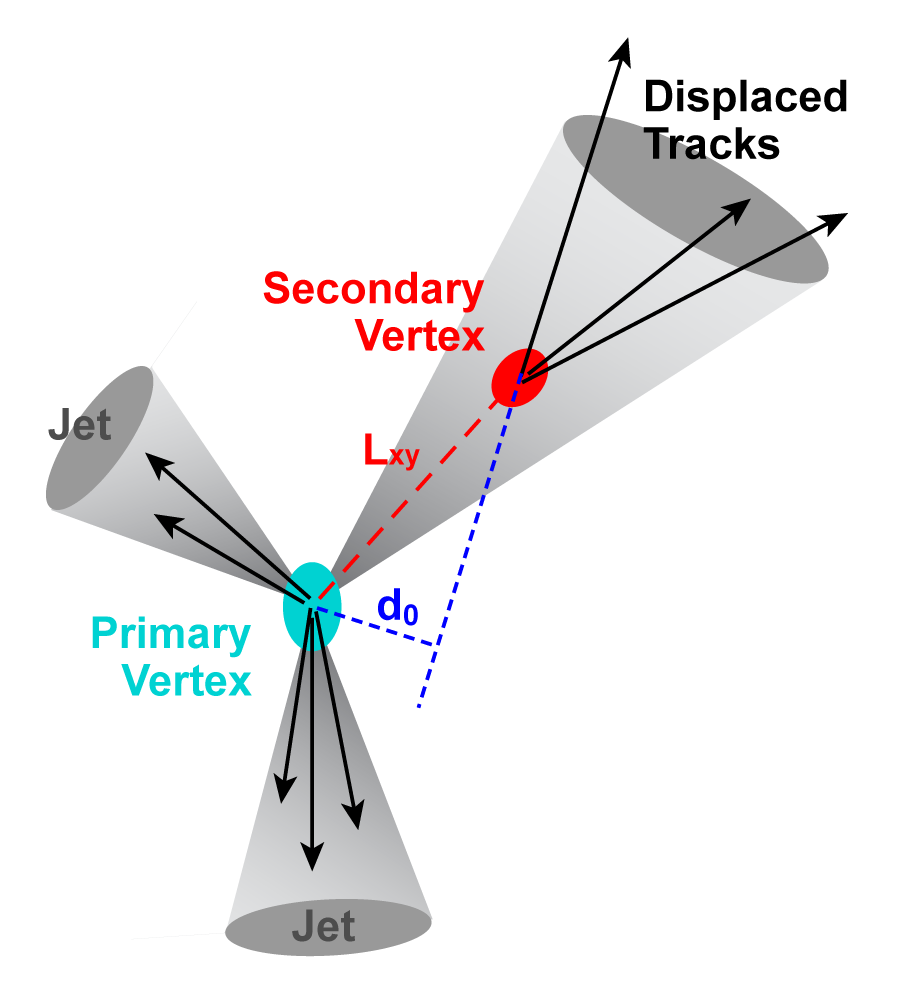
\includegraphics[width=0.8\textwidth]{Chapters/06_BTag_Study/Images/b_tagging_graphic}\\
     \caption[Graphical representation of a secondary vertex.]{Graphical representation of an
     interaction originating at the primary vertex producing three jets, one of which is a \bjet with a
     secondary vertex~\cite{d0_fnal}.}
     \label{fig:secondary_vertex}
\end{figure}

The impact parameter (IP) of a track is defined as the distance between the track and the vertex at the point
of closest approach~\cite{CMS-PAS-BTV-09-001}. Figure~\ref{fig:impact_parameter} shows a schematic
representation of the impact parameter for one single track. The IP measurement can be made in either the
plane transverse to the beam line, or in three dimensions. The impact parameter significance
(IP/$\sigma_{IP}$) is often used instead as an input to \btagging algorithms to allow for the experimental
resolution, due to the fact that the uncertainty on the IP value alone can be as large as the IP itself. The
IP significance distribution of light jets ($\cPqu$, $\cPqd$, $\cPqs$) and gluon jets form a Gaussian
distribution about a mean of zero and width of one, with a slightly extended tail due to tracks from particles
in the jet with long lifetimes. The equivalent distribution for \cjets and \bjets show an asymmetric
distribution at positive values due to the long lifetime of B and C hadrons, making the IP significance a
useful parameter to distinguish between light and heavy flavour jets~\cite{CMS-AN-2005-041}.

The signed IP is also used, in which the sign is obtained from the sign of the scalar product of the IP vector
and the jet direction, so that it is positive if the angle between the IP vector and the jet direction is less
than 90$^{\circ}$, and negative if the angle is greater than 90$^{\circ}$. Tracks belonging in a \bjet would
have an IP sign >0, since the jet direction is an estimate of the direction of travel of the B hadron.
However, the sign could be inaccurately calculated in cases with badly reconstructed jet directions or primary
vertices, or badly measured track parameters~\cite{CMS-AN-2005-041}. Another parameter based on track length,
the 3D decay length significance (the ratio of the three dimensional distance between the primary vertex and
the secondary vertex, and the uncertainty on this value) is also used by some \btagging algorithms.

\begin{figure}[hbtp]
   \centering
     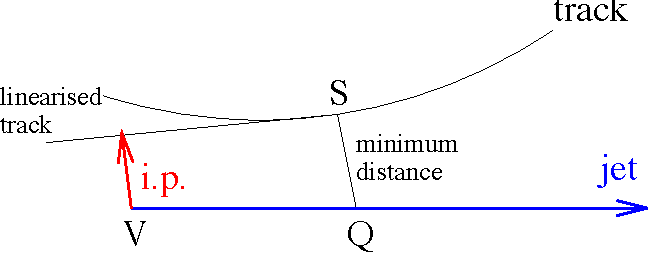
\includegraphics[width=0.8\textwidth]{Chapters/06_BTag_Study/Images/impact_parameter}\\
     \caption[Graphical representation of a track impact parameter.]{Graphical representation of a track
     impact parameter~\cite{CMS-PAS-BTV-09-001}.}
     \label{fig:impact_parameter}
\end{figure}

Identification of vertices in CMS consists of two stages: vertex finding and vertex fitting. Vertex finding
deals with the creation of vertex candidates by grouping reconstructed tracks together. Vertex fitting then
deals with obtaining the vertex parameters such as vertex position, track parameters, and quality of the fit.
An adaptive vertex fitter~\cite{0954-3899-34-12-N01} calculates an estimate of the vertex position and weights
tracks based on their compatibility with the vertex. This fit is initially constrained to the interaction
region to identify prompt tracks. After removing tracks with weights >0.5, subsequent fits are carried out to
identify potential decay vertices, until no new vertex is identified.

% The following requirements are placed on
% reconstructed tracks:
% \begin{itemize}
%   \item $\pt>1\GeV\c$
%   \item $\geq2$ reconstructed hits in the pixel tracker
%   \item $\geq8$ reconstructed hits in whole the tracker (pixels and strips)
%   \item $\chi^{2}/dof<10$
%   \item impact parameter of the track with respect to the primary vertex <2\mm
%   \item tracks are included in a jet if they are within a cone of $\DeltaR<0.3$ of the jet axis
% \end{itemize}

\section{\texorpdfstring{\btagging}{b-tagging} algorithm descriptions}
\label{s:btagging_algorithm_descriptions}

\subsection{Track Counting}
\label{ss:track_counting}
The simplest \btagging algorithms available in CMS are the track counting
algorithms~\cite{CMS-PAS-BTV-09-001}, which positively identifies a \bjet if it contains N or more tracks with
IP significance above some threshold value. They function by ordering all good tracks in a jet by order of
decreasing IP significance, with the discriminator being the IP significance of the Nth track. The high
efficiency version of this algorithm uses N=2, i.e. the second track, and the high purity version uses N=3,
i.e. the third track~\cite{CMS-AN-2005-041}.

\subsection{Jet Probability}
\label{ss:jet_probability}
The ``jet probability'' algorithms~\cite{CMS-PAS-BTV-09-001} produce a discriminator based on the probability that
the set of tracks come from the primary vertex: a high probability would indicate that the jet is not a \bjet,
which would originate at a secondary vertex. These algorithms use all tracks as input and for each track
define an individual probability of coming from the primary vertex. By combining these probabilities, a jet
probability is produced, and the discriminator is the negative log of this confidence
level~\cite{CMS-AN-2005-041}. The ``jet B probability'' variant is based on the confidence level that the four
most displaced tracks in the jet originate from the primary vertex. The four most displaced tracks are
used since the average number of tracks in a \bjet is approximately 5, and the reconstruction of tracks within
jets has an average efficiency of approximately 80\%~\cite{CMS-PAS-BTV-09-001} (the track reconstruction
efficiency is $\approx80\%$ for tracks of \pt=0.5\GeV, increasing to $\approx90\%$ for tracks of
\pt=10\GeV~\cite{Khachatryan:2015lha}).

\subsection{Soft Muon}
\label{ss:soft_muon}
The ``soft muon'' algorithms make use of global muons reconstructed in the vicinity of the reconstructed jet,
which may indicate a semi-leptonic decay of B hadrons to a muon~\cite{CMS-AN-2009-085}. Two soft muon
algorithms exist in CMS. The ``soft muon by \pt'' algorithm uses the relative \pt of the muon with respect to
the jet ($p_{T(rel)}$), which is expected to be larger than that for muons in light flavour jets due to the
large \bquark mass~\cite{CMS-AN-2009-085, Ferro:2012tg}. A ``soft muon by IP algorithm'' also exists which
uses the IP significance of positive IP muons. In jets containing more than one muon, the muon with the
highest discriminator is used.

\subsection{Simple Secondary Vertex}
\label{ss:simple_secondary_vertex}
The simple secondary vertex (SSV) algorithm uses the Adaptive Vertex Fitter to reconstruct the secondary
vertex~\cite{0954-3899-34-12-N01}. The discriminator is calculated based on the 3D decay length significance.
If no secondary vertex is reconstructed, no discriminator is produced, meaning that the efficiency of this
algorithm is limited to the maximum efficiency of secondary vertex reconstruction (approximately
65~\%)~\cite{Chatrchyan:2012jua}. There are two variants of the simple secondary vertex algorithm: the high
efficiency version uses vertices with at least two compatible tracks, whereas the high purity version uses
vertices with at least three tracks.

\subsection{Combined Secondary Vertex}
\label{ss:combined_secondary_vertex}
The current CMS recommendation for physics analyses (and therefore the algorithm used in the differential
cross section analysis presented in
Chapters~\ref{c:Differential_Cross_Section:data_simulation_and_selection}\textendash\ref{c:Differential_Cross_Section:systematics_and_results})
is the Combined Secondary Vertex (CSV) algorithm~\cite{Weiser:2006md}. This algorithm reconstructs the event
vertices using the Trimmed Kalman Vertex Finder~\cite{Speer:927395}, a vertex finding algorithm that fits
tracks to a primary vertex after removing incompatible tracks and applies the following cuts to these vertices
in order to find a secondary vertex.

\begin{itemize}
  \item the transverse distance between the primary and secondary vertices, $L_{T}$, must be $\geq100\um$ and
  $\leq2.5\cm$.
  \item $L_{T}$ divided by its error, $\sigma L_{T}$, must be $\geq3$.
  \item all charged particles related to the vertex must have an invariant mass of $\leq6.5\GeV/c^{2}$.
  \item the vertex is rejected if it has two oppositely charged tracks within a mass window of $50\MeV/c^{2}$,
  in order to suppress the selection of vertices compatible with a $K_{S}^{0}$ decay.
\end{itemize}

The CSV algorithm then combines the following track-based lifetime parameters and secondary vertex information
to produce a discriminator~\cite{Weiser:2006md}:
\begin{itemize}
  \item IP and IP significance
  \item Flight distance significance
  \item Number of charged tracks in the jet (\bjets have a higher track multiplicity than, \eg \cjets)
  \item Invariant mass of charged particles related to the secondary vertex (seccondary \bjet vertices have a
  significcantly highger invariant mass than \cjets).
  \item Rapidities of charged particle tracks related to the secondary vertex.
\end{itemize}
All of the input variables are combined into the final discriminating variable using a likelihood technique.
The increased number of input parameters for the CSV algorithm means that even in cases with no reconstructed
secondary vertex a discriminator can be produced, thereby increasing the maximum efficiency compared to the
SSV algorithms~\cite{Chatrchyan:2012jua}.

As with all \btagging algorithms, a discriminator ranging from 0 to 1 is produced, with larger numbers
corresponding to a higher probability of a jet being a \bjet. Three \btagging working points are used in CMS:
tight, medium and loose. The medium working point is used in the differential cross sections analysis, which
carries a 1~\% mis-tag rate (the rate at which non-\bjets are mistakenly tagged as \bjets) and approximately
70~\% \btag efficiency. The tight and loose working points have mis-tag rates of 0.1~\% and 10~\%
respectively~\cite{Chatrchyan:2012jua}. The CSV MVA algorithm is a variant of this method, in which a
multi-variate analysis (MVA) is performed using the CMSSW MVA Tools to produce a discriminator.

\section{Performance Comparison}
\label{s:performance_comparison}

Distributions of the discriminators produced by the above algorithms were created for a \ttbar \MADGRAPH Monte
Carlo simulation sample (/TTJets\_TuneZ2\_7TeV-madgraph-tauola/, produced in the Fall2011 production cycle
using CMSSSW version 44X). A comparison of the discriminator distributions, after normalising to unit area,
for the described algorithms were carried out. Figure~\ref{fig:CSV_discriminators} shows a comparison between
the distributions obtained by the CSV algorithm for the different jets present in the sample: \bjets, light
jets (up, down and strange flavour: \udsjets), gluon jets (\gjets) and charm flavour jets (\cjets). All
distributions were normalised to unity in order to facilitate shape comparison. Equivalent plots for other
algorithms are included in Figure~\ref{fig:all_algorithm_discriminators} in Appendix~\ref{ac:b_tagging_plots}.
In all cases, it can be seen that higher discriminator values were produced for \bjets than for \udsjets,
\gjets and \cjets, as expected.

\begin{figure}[hbtp]
   \centering
     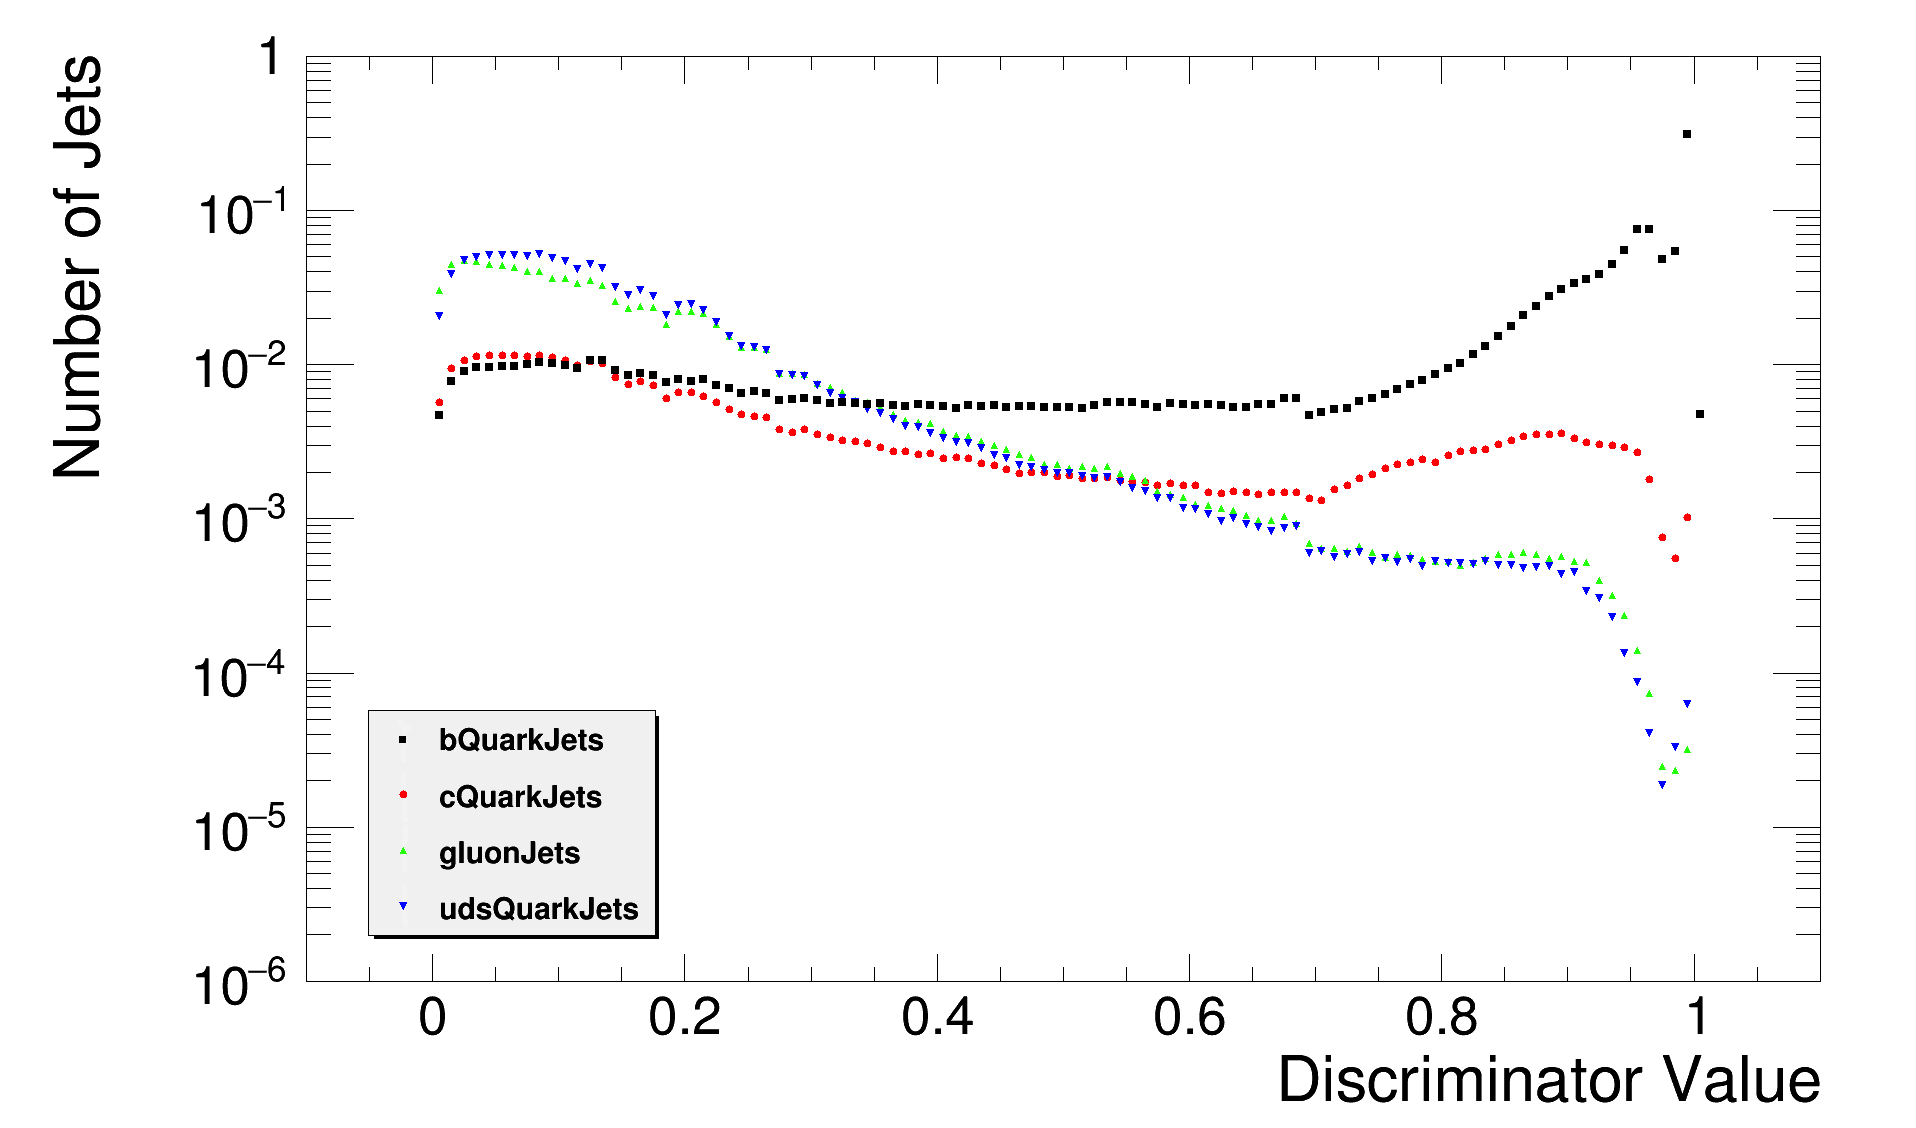
\includegraphics[width=\textwidth]{Chapters/06_BTag_Study/Images/CombinedSecondaryVertex_norm_discriminator_combined}\\
     \caption[Discriminator values produced by the Combined Secondary Vertex algorithm after
     normalisation.]{Discriminator values produced by the Combined Secondary Vertex algorithm for all \bjets,
     \cjets, \gjets and \udsjets after normalisation.}
     \label{fig:CSV_discriminators}
\end{figure}

\section{Efficiency}
\label{s:efficiency}

Analyses in CMS make use of \btagging algorithms by placing cuts on the discriminators. The efficiency of a
cut can be defined as the ratio of number of jets passing the selection cut to the total number of jets before
the selection cut. The efficiency was calculated for cut values spanning the whole range of discriminator
values, and the resulting plot of \btagging efficiency for non-\bjets as a function of \btagging efficiency
for \bjets is shown Figure~\ref{fig:CSV_jet_efficiencies}. In practice, the aim is to achieve a high \bjet
efficiency and a low efficiency for all other jet flavours, \ie the lower right region of the plot. It can be
seen that \udsjets and \gjets have similar rates of increase in efficiencies with respect to cut value, owing
to their similar discriminator distributions. The \cjet discriminator distribution
(Figure~\ref{fig:CSV_discriminators}), however, has a noticeably different shape. This leads to the
undesirable trend of higher \cjet efficiencies than for \udsjets and \gjets. Equivalent plots for other
algorithms can be found in Figure~\ref{fig:all_algorithm_efficiencies} in Appendix~\ref{ac:b_tagging_plots}.

\begin{figure}[hbtp]
   \centering
     \includegraphics[width=\textwidth]{Chapters/06_BTag_Study/Images/CombinedSecondaryVertex_nonBJetEfficiency_v_bJetEfficiency}\\
     \caption[\btagging efficiencies of non-\bjets as a function of \btagging efficiency for \bjets for the
     CSV algorithm.]{\btagging efficiencies of non-\bjets as a function of \btagging efficiency for \bjets for
     the CSV algorithm.}
     \label{fig:CSV_jet_efficiencies}
\end{figure}

\section{Algorithm Comparison}
\label{algorithm_comparison}

The performances of the various algorithms can be compared in Figure~\ref{fig:uds_eff_v_b_eff}.

\begin{figure}[hbtp]
   \centering
     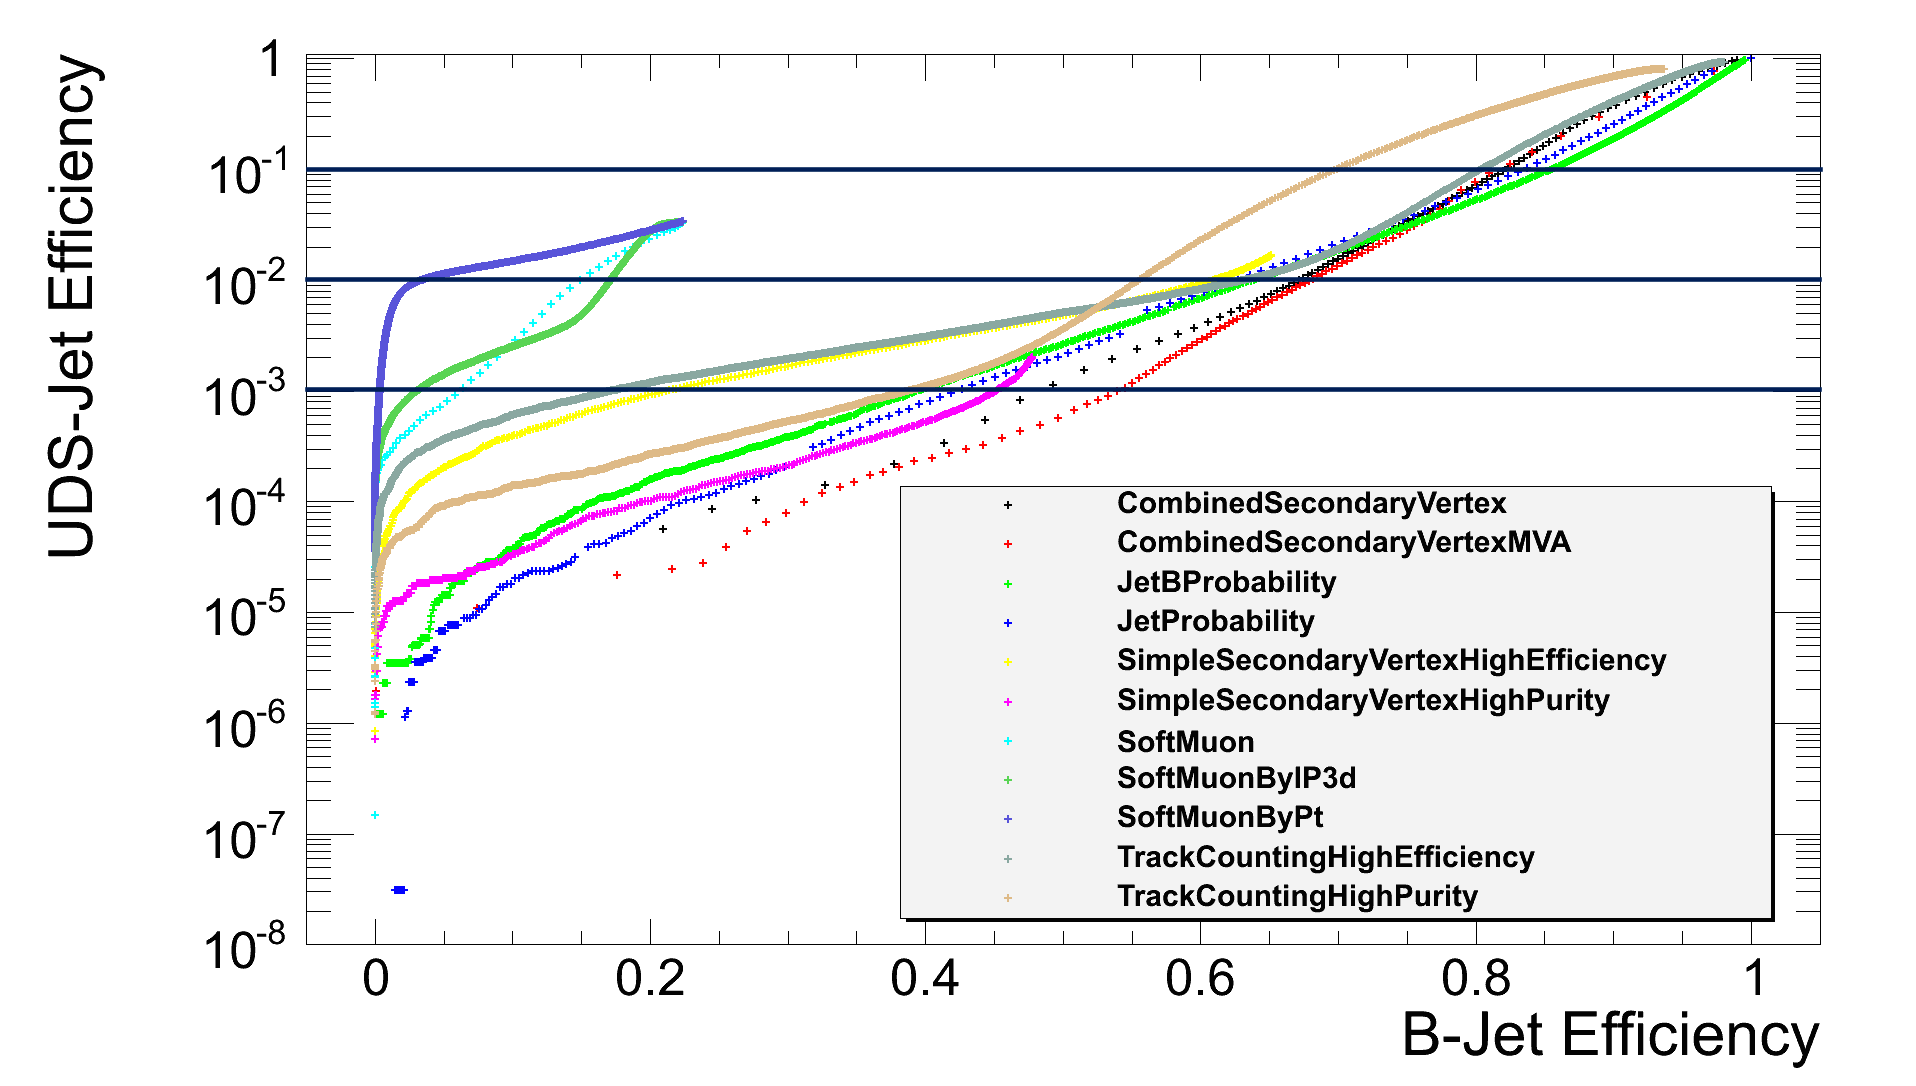
\includegraphics[width=\textwidth]{Chapters/06_BTag_Study/Images/udsJetEfficiency_v_bJetEfficiency_withLegend_wp}\\
     \caption[udsjet efficiencies as a function of \bjet efficiencies for all algorithms.]{\udsjet
     efficiencies as a function of \bjet efficiencies for all algorithms.}
     \label{fig:uds_eff_v_b_eff}
\end{figure}

It can be seen that not all algorithms reach 100~\% \bjet efficiency due to being inherently limited by their
methods. For example, the soft muon algorithms are limited by the muon identification efficiency within \bjets
and also by the branching fraction of B hadrons to muons. The soft muon algorithms all show low maximum \bjet
efficiencies due to the low B hadron semi-leptonic branching ratio to muons of approximately 11~\% (or 20~\%
when further decays are included such as $\cPqb \rightarrow \cPqc \rightarrow l$) \cite{Ferro:2012tg}.
Similarly, the SSV algorithms are limited by the efficiency of reconstructing a secondary vertex in the jet of
approximately 65~\%.

The 2011 and 2012 CMS recommended \btagger is the CSV algorithm with operating point discriminator
cuts of 0.244 (loose), 0.679 (medium) and 0.898 (tight) corresponding to 10\%, 1\% and 0.1\% light jet
efficiencies. These cuts are indicated by the horizontal lines on Figure~\ref{fig:uds_eff_v_b_eff}. It can be
seen that for the tight and medium cuts, the CSV MVA algorithm provides the highest \bjet efficiency and
lowest light jet efficiency, followed closely by the CSV algorithm. The multiple variables (see
Section~\ref{ss:combined_secondary_vertex}) that are used as input allow the CSV algorithm to produce higher
efficiencies than the SSV algorithms, while the MVA analysis variant provides a slightly improved performance.
At approximately 3~\% light jet efficiency, there is a convergence of many algorithms that all provide similar
performance. At the loose working point also, many of the algorithms provide similar performance with \bjets,
with the ``jet probability'' algorithms marginally outperforming the CSV algorithms. In early CMSSW versions,
it was known that the jet probability algorithm provided optimal performance, leading to it being recommended
for early CMS analyses. Ultimately, the CSV algorithm provides better performance in CMSSW versions after
CMSSW\_2\_X\_Y, at which point it became the recommended \btagging method.

\chapter{Differential Cross Sections: Data, Simulation and Selection}
\label{c:Differential_Cross_Section:data_simulation_and_selection}

\section{Outline and Motivation}
\label{s:outline_and_motivation}
This chapter describes the first part of the main \ttbar differential cross section analysis in bins of global
event variables. Following an introduction to the variables under investigation and motivations, the datasets
used and the selection process is explained, including scale factors and corrections applied to ensure
agreement between Monte Carlo simulation and data.

The analysis measures the normalised differential \ttbar cross section in the semi-leptonic channel and is
carried out on 2011 and 2012 data recorded from the CMS detector. The measurement is carried out with respect
to the following global, or primary, variables:
\begin {itemize}

  \item {\met, the missing transverse energy in an event, defined as the magnitude of the missing transverse
  momentum vector \ptvecmiss (which is defined as the projection of the negative vector sum of the momenta of
  all PF objects in the event on the plane perpendicular to the beams).}
  	\[\met = \left[ \left(\sum_i{p_{x}^i}\right)^2 + \left(\sum_i{p_{y}^i}\right)^2 \right]^{\frac{1}{2}},\]
  	where $p_x^i$ and $p_yi$ are momentum components of the \textit{i}th object in the event, and the sums
  	include all PF objects in the event, with no lower threshold applied. See Section~\ref{ss:met_corrections}
  	for details of corrections applied in the calculation of this \met, which include, amongst others,
  	propagation of jet energy corrections and takes account of pileup interactions.

  \item {\HT, the sum of the transverse momenta of all jets with $\pt>20\GeV$ and $\abseta<2.5$ in an
  event}
  	\[\HT = \sum_{\text{all jets}}\pt^{\mathrm{jet}}\].

  \item {\st, the sum of all observed transverse momenta in an event, \ie the scalar sum of \HT, \met, and
  	lepton \pt}
  	\[\st = \HT + \met + p_\mathrm{T}^\mathrm{lepton}.\]

  \item {\wpt, the transverse momentum of the leptonically decaying \W boson, obtained from \ptvecmiss and the
  \pt of the lepton}
	\[\wpt = \sqrt{\left(p_x^{\mathrm{lepton}} + p_x^{\mathrm{miss}}\right)^2 + \left(p_y^{\mathrm{lepton}} +
	p_y^{\mathrm{miss}}\right)^2},\]
	where $p_{x}^{\mathrm{lepton}}$ and $p_{y}^{\mathrm{lepton}}$ are the transverse components of
	$\vec{p}^{\mathrm{lepton}}$, and $p_x^{\mathrm{miss}}$ and $p_y^{\mathrm{miss}}$ are the transverse
	components of \ptvecmiss.

  \item {\mt, the transverse mass of the leptonically decaying \W boson, also obtained from \met and the \pt
  of the lepton}
    \[\mt = \sqrt{\et\left(\text{lepton}, \met\right)^{2} - (\wpt)^{2}},\]
    where $\et\left(\text{lepton}, \met\right)$ is the scalar sum of \met and the transverse energy of the
    lepton, \ie $\met + \et^{\text{lepton}}$
 
\end{itemize}

The central objective of these measurements is to verify the models and generators used to produce simulations
of the signal and background events in CMS. This understanding is important to provide a good foundation for
new physics analyses, where such events constitute a significant background. Comparison of results with
predictions using varied choices of the matching threshold of partons, and the renormalisation and
factorisation scale ($Q^{2}$) allow the verification of these model parameters used in event generation. In
addition, the distributions under investigation may be sensitive to rare standard model processes; for
example, the \met and \mt distributions could show signs of \ttbar+\Z (where $Z\rightarrow \nu\bar{\nu}$)
and/or \ttbar+\W (where $W\rightarrow l\nu$) processes, which produce additional \met. The \wpt and \mt
distributions are related to the leptonically decaying \W boson, and therefore give a handle on modelling of
the transverse momentum of the relevant top quark. The \HT and \st distributions would provide information on
\ttbar+X production where X is massive and decays to hadrons. Hints of new physics scenarios such as stop pair
production, $\tilde{t}\bar{\tilde{t}} \rightarrow t\tilde{\chi_0} \bar{t}\bar{\tilde{\chi_0}}$, where
$\tilde{\chi_0}$ is the lightest supersymmetric particle and a possible dark matter candidate, may also be
visible in the distributions of global variables. Cases of rare SM processes or new physics are likely to
manifest as observed excesses over predictions in the tails of the primary variables, making this region of
the distributions of particular interest.

Note that this analysis on the aforementioned global variables does not require reconstruction of the \ttbar
decay to identify which decay products are associated with each top quark, and is intended as a complementary
analysis to other CMS studies in which such reconstruction is carried out.

\section{Data and Simulated Samples}
\label{s:data_and_simulated_samples}

\subsection{Data}
\label{ss:data}

Data collected in 2011 at a centre-of-mass energy of 7\TeV corresponding to an integrated luminosity of
5.0\fbinv, and in 2012 at a centre-of-mass energy of 8\TeV corresponding to an integrated luminosity of
19.7\fbinv are used in this analysis. The datasets are determined by the triggers that were used to record
them. For 7\TeV, the ``ElectronHad'' dataset is used in the electron channel, which was recorded with triggers
that select events based on at least one, isolated electron and additional jets. At 8\TeV, the
``SingleElectron'' dataset was used for the electron channel which is based only on at least one, isolated
electron. In the muon channel, the ``SingleMu'' dataset was used for both centre-of-mass energies, requiring a
single, isolated muon.

These datasets are produced from CMS data by requiring events to pass a trigger. The triggers used in both
7\TeV and 8\TeV data are shown in Table~\ref{tab:HLTTriggers} in Appendix~\ref{as:datasets}. In the electron
channel, an electron+jets trigger was used in 2011 with a requirement of at least one electron with
\Et$>25\GeV$ and at least three jets with \pt$>30\GeV$; and a single electron trigger was used in 2012 with at
least one electron with \Et$>27\GeV$. In the muon channel, a single muon trigger was used in both data taking
periods with a requirement of at least one muon with \pt$>24\GeV$. In addition to these kinematic
requirements, the triggers also have cuts on the ratio between the HCAL and the ECAL energy ($H/E$), track matching with
ECAL ($\Delta\eta$ and $\Delta\phi$), cluster shape ($\sigma_{i\eta i\eta}$), ECAL isolation
($\frac{\text{ECAL iso}}{E_\text{T}}$), HCAL isolation ($\frac{\text{HCAL iso}}{E_\text{T}}$) and tracker
isolation ($\frac{\text{tracker iso}}{\pt}$). In both channels, the final selection is tighter than these
trigger requirements.

The datasets used are shown in Tables~\ref{tab:datasets7TeV} and \ref{tab:datasets8TeV}.Only data that is
certified as ``golden'' (data taken with the CMS detector working without any major faults) is used. The masks
used to filter out data taken in other periods are specified in Table~\ref{tab:JSONfiles} in
Appendix~\ref{as:datasets}.

\begin{table}[hbth]
\centering
\begin{tabular}{llrr}
\hline
\textbf{Data set name} & \textbf{Run period} & \textbf{$\mathbf{\mathcal{L}_{int}}$ / \pbinv} & \textbf{Runs}
\\
\hline
ElectronHad 12 Oct 2013 ReReco & Run2011A & 2,333 & 160404--173692 \\
ElectronHad 12 Oct 2013 ReReco & Run2011B & 2,738 & 175833--180252 \\
\hline
SingleMu 12 Oct 2013 ReReco & Run2011A & 2,331 & 160404--173692 \\
SingleMu 12 Oct 2013 ReReco & Run2011B & 2,766 & 175833--180252 \\
\hline
\end{tabular}
\caption{7 TeV data sets by run period with the corresponding integrated
luminosities ($\mathcal{L}_{int}$) and run numbers.}
\label{tab:datasets7TeV}
\end{table}
\begin{table}[hbth]
\centering
\begin{tabular}{llrr}
\hline
\textbf{Data set name} & \textbf{Run period} & \textbf{$\mathbf{\mathcal{L}_{int}}$ / \pbinv} & \textbf{Runs}
\\
\hline
SingleElectron 22 Jan 2013 ReReco & Run2012A & $883.3$ & 190456--193621 \\
SingleElectron 22 Jan 2013 ReReco & Run2012B & $4,389.0$ & 193834--196531 \\
SingleElectron 22 Jan 2013 ReReco & Run2012C & $7,137.0$ & 198022--203742 \\
SingleElectron 22 Jan 2013 ReReco & Run2012D & $7,318.0$ & 203777--208686 \\
\hline
SingleMu 22 Jan 2013 ReReco & Run2012A & $889.4$ & 190456--193621 \\
SingleMu 22 Jan 2013 ReReco & Run2012B & $4,424.0$ & 193834--196531 \\
SingleMu 22 Jan 2013 ReReco & Run2012C & $7,152.0$ & 198022--203742 \\
SingleMu 22 Jan 2013 ReReco & Run2012D & $7,280.0$ & 203777--208686 \\
\hline
\end{tabular}
\caption{8 TeV data sets by run period with the corresponding integrated
luminosities ($\mathcal{L}_{int}$) and run numbers.}
\label{tab:datasets8TeV}
\end{table}

\FloatBarrier

\subsection{Simulated Samples}
\label{ss:simulated_samples}
The signal event for this analysis is the production of a \ttbar pair which decays semi-leptonically, \ie each
of the \tquarks decays to a \W boson and a \bjet, with one of the \W bosons decaying hadronically to two jets
and the other decaying leptonically to a lepton (electron or muon) and an associated neutrino.
Section~\ref{c:top_physics_at_the_lhc} outlines the signal and background events considered. Additional, lower
energy jets, can be produced from other scatterings in the same proton-proton interaction and from gluon
radiation from quarks in the decay. See Section~\ref{c:top_physics_at_the_lhc} for detailed descriptions of
the signal and backgrounds in this analysis.

The Monte Carlo generators used in this analysis are \MADGRAPH v5.1.5.11~\cite{madgraph5}, \PYTHIA
v6.426~\cite{Sjostrand:2006za}, \POWHEG v1.0, r1380 and \POWHEG v2.0,
r2819~\cite{Nason:2004rx,Frixione:2007vw,Alioli:2010xd}, \HERWIG v6.520~\cite{herwig} and \MCATNLO
v3.41~\cite{Frixione:2002ik,Frixione:2003ei}. See Section~\ref{s:monte_carlo_simulation} for details about
these Monte Carlo generators. The \GEANTfour package~\cite{Agostinelli:2002hh,Allison:2006ve} is used to
simulate the CMS detector response.

Tables~\ref{tab:signaldatasets7TeV} and~\ref{tab:signaldatasets8TeV} show the Monte Carlo signal samples used
in this analysis at 7\TeV and 8\TeV respectively. Tables~\ref{tab:backgrounddatasets7TeV}
and~\ref{tab:backgrounddatasets8TeV} list the background simulation samples used.

Top pair production is modelled using the \MADGRAPH event generator, with \PYTHIA modelling the parton
showering and hadronisation, with matching between the parton showers and the matrix element performed via the
MLM prescription~\cite{Hoche:2006ph} (Section~\ref{ss:madgraph}). Two independent \ttbar samples are also
produced with the \POWHEG2 generator interfaced with \PYTHIA and \HERWIG for parton showering. At
$\roots=7\TeV$, three additional samples are used generated using \MCATNLO with \HERWIG to model the parton
showers, \POWHEG1 with \PYTHIA, and \POWHEG1 with \HERWIG.

Single top events are modelled with \POWHEG, \W and \Z boson plus jets production is modelled using \MADGRAPH
and QCD multi-jet events are modelled with \PYTHIA. Tables~\ref{tab:7TeVsystematicdatasets} and
\ref{tab:8TeVsystematicdatasets} show the samples used to evaluate the factorisation scale, matching
threshold, and top quark mass uncertainties. \WpJets and \ZpJets samples were not made available at 7\TeV, so
the scaled distributions from 8\TeV were used, as described in
Section~\ref{sss:7TeV_vjets_theory_systematic_template}.

Standard Model cross sections at NNLO of 252.89\pb at $\roots=7\TeV$ and 177.31\pb at $\roots=8\TeV$ are used
for \ttbar processes~\cite{Czakon:2013goa}. NNLO cross sections are also applied for\WpJets processes and
\ZpJets processes~\cite{Melnikov:2006kv}. Cross sections at NLO are used for single top
processes~\cite{Campbell:2009ss} and LO cross sections are used for QCD multi-jet processes. Numerical values
for cross sections are included in all abovementioned tables.

The CTEQ6L PDFs~\cite{Pumplin:2002vw} are used to generate the \MADGRAPH simulations, the CT10
PDFs~\cite{ct10} are used for \POWHEG production and CTEQ6M PDFs~\cite{Pumplin:2002vw} are used for \MCATNLO.
The underlying event tunes (sets of theory parameters) used for production of the \MADGRAPH and \POWHEGPYTHIA2
samples at $\roots=7\TeV$, as well as the \MCATNLOHERWIG sample at $\roots=8\TeV$, is the \PYTHIA Z2
tune~\cite{Z2UE}. The \PYTHIA Z2* is used for the \MADGRAPH, \POWHEGPYTHIA1 and \POWHEGPYTHIA2 samples at
$\roots=8\TeV$, and the AUET tune~\cite{AUET2UE} is used in all \POWHEGHERWIG samples. All simulations are
generated with a top quark mass of 172.5\GeV, and in all cases, \PYTHIA is used to model parton showering,
radiation and hadronisation processes.

\begin{table}[hbth]
\centering
\caption{7\TeV Monte Carlo signal datasets used for this analysis.}
\label{tab:signaldatasets7TeV} \small\addtolength{\tabcolsep}{-5pt}
\begin{tabular}{llrrr}
%\multicolumn{6}{c}{Signal datasets}
%\hline
Process & Generator & $\sigma$/$\pb$ & No. events & \lumiint/$\fbinv$ \\
\hline
\ttbar & \MADGRAPH & 177.31 & 17100187 & 96.4 \\
\ttbar & \MCATNLO & Not Available & - & - \\
\ttbar & \POWHEGPYTHIA1 & Not Available & - & - \\
\ttbar & \POWHEGHERWIG1 & Not Available & - & - \\
\ttbar & \POWHEGPYTHIA2 & 177.31 & 4833135 & 27.3 \\
\ttbar & \POWHEGHERWIG2 & 177.31 & 4480816 & 25.3 \\
\hline
\end{tabular}
\end{table}


\begin{table}[hbth]
\centering
\caption{8\TeV Monte Carlo signal datasets used for this analysis.}
\label{tab:signaldatasets8TeV} \small\addtolength{\tabcolsep}{-5pt}
\begin{tabular}{llrrr}
%\multicolumn{6}{c}{Signal datasets}
%\hline
Process & Generator & $\sigma$/$\pb$ & No. events & \lumiint/$\fbinv$ \\
\hline
\ttbar & \MADGRAPH & 252.89 & 6706068 & 26.5 \\
\ttbar & \MCATNLO & 252.89 & 32852517 & 129.9 \\
\ttbar & \POWHEGPYTHIA1 & 252.89 & 21675913 & 85.7 \\
\ttbar & \POWHEGHERWIG1 & 252.89 & 27684194 & 109.5 \\
\ttbar & \POWHEGPYTHIA2 & 252.89 & 9044049 & 35.8 \\
\ttbar & \POWHEGHERWIG2 & 252.89 & 8630382 & 34.1 \\
\hline
\end{tabular}
\end{table}


\begin{table}[hbth]
\centering
\caption{\SI{7}{\TeV} Monte Carlo background datasets used for this analysis. All samples are generated
inclusively if not marked otherwise ($^\star$ generator cut on in-flight-decays of b- and c-hadrons, $^\ominus$ enriched in conversion electrons; $l$ means
all leptonic decays: $l=e,\mu,\tau$; $^\bullet$ generator cut on $m_{Z/\gamma} > 50$~GeV).
\label{tab:backgrounddatasets7TeV}} \small\addtolength{\tabcolsep}{-5pt}
\begin{tabular}{llrrr}
%\multicolumn{6}{c}{Background datasets} 
%\hline
Process & Generator & $\sigma$ ($\pb$) & No. events & \lumiint ($\fbinv$) \\
\hline
\hline
Single \cPqt t-channel ($W\rightarrow l\nu$) & \POWHEG & 42.6 & 3249530 & 76.3 \\
Single \cPaqt t-channel ($W\rightarrow l\nu$) & \POWHEG & 22.0 & 1813615 & 82.4 \\
Single \cPqt s-channel ($W\rightarrow l\nu$) & \POWHEG & 2.72 & 229786 & 84.5 \\
Single \cPaqt s-channel ($W\rightarrow l\nu$) & \POWHEG & 1.49 & 138187 & 92.7 \\
Single \cPqt tW-channel ($W\rightarrow l\nu$) & \POWHEG & 5.3 & 744859 & 140.5 \\
Single \cPaqt tW-channel ($W\rightarrow l\nu$) & \POWHEG & 5.3 & 801626 & 151.3 \\
\hline
\W ($\rightarrow l\nu$) + 1 Jet & \MADGRAPH & 4480.0 & 70430949 & 15.7 \\
\W ($\rightarrow l\nu$) + 2 Jets & \MADGRAPH & 1435.0 & 25069566 & 17.5 \\
\W ($\rightarrow l\nu$) + 3 Jets & \MADGRAPH & 304.2 & 6291772 & 20.7 \\
\W ($\rightarrow l\nu$) + 4 Jets & \MADGRAPH & 172.6 & 13240209 & 76.7 \\
\Z/$\photon^{*}$ ($\rightarrow l^+l^-$) + jets $^\bullet$ & \MADGRAPH & 3048 & 32846945 & 10.8 \\
\hline
QCD BCtoE \PT 20-30 $^\star$ & \PYTHIA & 139299.0 & 1927944 & 1.4$\times 10^{-2}$ \\
QCD BCtoE \PT 30-80 $^\star$ & \PYTHIA & 143844.8 & 1946505 & 1.4$\times 10^{-2}$ \\
QCD BCtoE \PT 80-170 $^\star$ & \PYTHIA & 9431.1 & 1002427 & 0.1 \\
\hline
QCD EM  \PT 20-30 $^\ominus$ & \PYTHIA & 2502660.0 & 32976415 & 1.3$\times 10^{-2}$ \\ 
QCD EM \PT 30-80 $^\ominus$ & \PYTHIA & 3625840.0 & 71775065 & 2.0$\times 10^{-2}$ \\
QCD EM \PT 80-170 $^\ominus$ & \PYTHIA & 142813.8 & 7650319 & 5.4$\times 10^{-2}$ \\
QCD EM  \PT 170-250 $^\ominus$ & \PYTHIA & 142813.8 & 2968842 & 2.1$\times 10^{-2}$ \\
QCD EM  \PT 250-350 $^\ominus$ & \PYTHIA & 368.0 & 2952960 & 8.0 \\
QCD EM \PT 350-inf $^\ominus$ & \PYTHIA & 55.0 & 2957326 & 53.8 \\
\hline
$\gamma$ + Jets HT 40-100 & \MADGRAPH & 25690.0 & 9882860 & 0.4 \\
$\gamma$ + Jets HT 100-200 & \MADGRAPH & 5213.0 & 1514347 & 0.3 \\
$\gamma$ + Jets HT $>$ 200 & \MADGRAPH & 798.3 & 9275592 & 11.6 \\
\hline
QCD $\mu$ enriched \PT 15-20 & \PYTHIA & 1668096.0 & 1901684 & 1.1$\times 10^{-3}$ \\
QCD $\mu$ enriched \PT 20-30 & \PYTHIA & 1342184.0 & 10173300 & 7.6$\times 10^{-3}$ \\
QCD $\mu$ enriched \PT 30-50 & \PYTHIA & 596506.8 & 11610111 & 1.9$\times 10^{-2}$ \\
QCD $\mu$ enriched \PT 50-80 & \PYTHIA & 140039.55 & 9870031 & 7.0$\times 10^{-2}$ \\
QCD $\mu$ enriched \PT 80-120 & \PYTHIA & 28546.2 & 9769136 & 0.3 \\
QCD $\mu$ enriched \PT 120-170 & \PYTHIA & 4692.91 & 7818474 & 1.7 \\
QCD $\mu$ enriched \PT 170-300 & \PYTHIA & 1445.96 & 8116409 & 5.6 \\
QCD $\mu$ enriched \PT 300-470 & \PYTHIA & 95.4464 & 7870002 & 82.5 \\
QCD $\mu$ enriched \PT 470-600 & \PYTHIA & 7.41697 & 3812529 & 514.0 \\
QCD $\mu$ enriched \PT 600-800 & \PYTHIA & 1.69145 & 4149911 & 2453.5 \\
QCD $\mu$ enriched \PT 800-1000 & \PYTHIA & 0.231869 & 4036867 & 17410.1 \\
QCD $\mu$ enriched \PT 1000-inf & \PYTHIA & 0.053385 & 4133897 & 77435.6 \\
\hline
\end{tabular}
\end{table}
\begin{table}[hbth]
\centering
\caption{\SI{8}{\TeV} Monte Carlo background datasets used for this analysis. All samples are generated
inclusively if not marked otherwise ($^\star$ generator cut on in-flight-decays of b- and c-hadrons, $^\ominus$ enriched in conversion electrons; $l$ means
all leptonic decays: $l=e,\mu,\tau$; $^\bullet$ generator cut on $m_{Z/\gamma} > 50$~GeV).
\label{tab:backgrounddatasets8TeV}} \small\addtolength{\tabcolsep}{-5pt}
\begin{tabular}{llrrr}
%\multicolumn{6}{c}{Background datasets} 
%\hline
Process & Generator & $\sigma$ ($\pb$) & No. events & \lumiint ($\fbinv$) \\
\hline
\hline
Single \cPqt t-channel ($W\rightarrow l\nu$) & \POWHEG & 55.53100 & 3758221 & 67.7 \\
Single \cPaqt t-channel ($W\rightarrow l\nu$) & \POWHEG & 30.00420 & 1906041 & 63.5 \\
Single \cPqt s-channel ($W\rightarrow l\nu$) & \POWHEG & 3.89394 & 259960 & 66.8 \\
Single \cPaqt s-channel ($W\rightarrow l\nu$) & \POWHEG & 1.75776 & 139974 & 79.6 \\
Single \cPqt tW-channel ($W\rightarrow l\nu$) & \POWHEG & 11.17730 & 497657 & 44.5 \\
Single \cPaqt tW-channel ($W\rightarrow l\nu$) & \POWHEG & 11.17730 & 473721 & 42.4 \\
\hline
\W ($\rightarrow l\nu$) + 1 Jet & \MADGRAPH & 5400.0 & 23129996 & 15.7 \\
\W ($\rightarrow l\nu$) + 2 Jets & \MADGRAPH & 1750.0 & 34027847 & 17.5 \\
\W ($\rightarrow l\nu$) + 3 Jets & \MADGRAPH & 519.0 & 15539463 & 20.7 \\
\W ($\rightarrow l\nu$) + 4 Jets & \MADGRAPH & 214.0 & 13373865 & 76.7 \\
\Z/$\photon^{*}$ ($\rightarrow l^+l^-$) + 1 jet$^\bullet$ & \MADGRAPH & 561.0 & 24032529 & 42.8 \\
\Z/$\photon^{*}$ ($\rightarrow l^+l^-$) + 2 jets$^\bullet$ & \MADGRAPH & 181.0 & 21840628 & 0.1 \\
\Z/$\photon^{*}$ ($\rightarrow l^+l^-$) + 3 jets$^\bullet$ & \MADGRAPH & 51.1 & 10819603 & 0.2 \\
\Z/$\photon^{*}$ ($\rightarrow l^+l^-$) + 4 jets$^\bullet$ & \MADGRAPH & 23.04 & 6381467 & 0.3 \\
\hline
QCD BCtoE \PT 20-30 $^\star$ & \PYTHIA & 167388.0 & 1731522 & 1.0$\times 10^{-2}$ \\
QCD BCtoE \PT 30-80 $^\star$ & \PYTHIA & 167040.0 & 2037907 & 1.2$\times 10^{-2}$ \\
QCD BCtoE \PT 80-170 $^\star$ & \PYTHIA & 12981.9 & 1945523 & 0.1 \\
QCD BCtoE \PT 170-250 $^\star$ & \PYTHIA & 632.0 & 1948112 & 3.1 \\
QCD BCtoE \PT 250-350 $^\star$ & \PYTHIA & 103.3 & 2026516 & 19.6 \\
QCD BCtoE \PT 350-inf $^\star$ & \PYTHIA & 23.9 & 1948525 & 81.5 \\
\hline
QCD EM  \PT 20-30 $^\ominus$ & \PYTHIA & 2914860.0 & 34830398 & 1.2$\times 10^{-2}$ \\ 
QCD EM \PT 30-80 $^\ominus$ & \PYTHIA & 4615893.0 & 32443607 & 7.0$\times 10^{-3}$ \\
QCD EM \PT 80-170 $^\ominus$ & \PYTHIA & 183294.9 & 34024542 & 0.2 \\
QCD EM  \PT 170-250 $^\ominus$ & \PYTHIA & 4586.5 & 31696985 & 6.9 \\
QCD EM  \PT 250-350 $^\ominus$ & \PYTHIA & 556.7 & 33659467 & 60.5 \\
QCD EM \PT 350-inf $^\ominus$ & \PYTHIA & 89.1 & 33756727 & 378.8 \\
\hline
$\gamma$ + Jets HT 200-400 & \MADGRAPH & 960.5 & 47316433 & 49.3 \\
$\gamma$ + Jets HT 400-inf & \MADGRAPH & 107.5 & 9491846 & 88.3 \\
\hline
QCD $\mu$ enriched \PT 15-20 & \PYTHIA & 2738580.0 & 1722678 & 0.6$\times 10^{-3}$ \\
QCD $\mu$ enriched \PT 20-30 & \PYTHIA & 1865500.0 & 8486893 & 4.5$\times 10^{-3}$ \\
QCD $\mu$ enriched \PT 30-50 & \PYTHIA & 806298.0 & 9560248 & 1.2$\times 10^{-2}$ \\
QCD $\mu$ enriched \PT 50-80 & \PYTHIA & 176187.6 & 10365209 & 5.9$\times 10^{-2}$ \\
QCD $\mu$ enriched \PT 80-120 & \PYTHIA & 40448.0 & 9238622 & 0.2 \\
QCD $\mu$ enriched \PT 120-170 & \PYTHIA & 7463.94 & 8501920 & 1.1 \\
QCD $\mu$ enriched \PT 170-300 & \PYTHIA & 2299.752 & 7669932 & 3.3 \\
QCD $\mu$ enriched \PT 300-470 & \PYTHIA & 151.8048 & 7832248 & 51.6 \\
QCD $\mu$ enriched \PT 470-600 & \PYTHIA & 11.79648 & 3783066 & 320.7 \\
QCD $\mu$ enriched \PT 600-800 & \PYTHIA & 2.690196 & 4118988 & 1531.1 \\
QCD $\mu$ enriched \PT 800-1000 & \PYTHIA & 0.3687810 & 4099633 & 11116.7 \\
QCD $\mu$ enriched \PT 1000-inf & \PYTHIA & 0.0849078 & 9238622 & 108807.7 \\
\hline
\end{tabular}
\end{table}

\begin{landscape}
\begin{table}[hbth]
\centering
\caption{7~\TeV Monte Carlo systematic datasets used for this analysis. All samples are produced with
the \MADGRAPH generator. \WpJets and \ZpJets samples were not available and so have been scaled from
available 8\TeV samples.}
\label{tab:7TeVsystematicdatasets} \small\addtolength{\tabcolsep}{-5pt}
\begin{tabular}{lllrrr}
%\multicolumn{6}{c}{Signal datasets}
%\hline
Process & Variation & Generator & $\sigma$ ($\pb$) & No. events & \lumiint ($\fbinv$) \\
\hline
\ttbar & 0.5$\times Q^{2}$ (norm. \& fact. scale down) & \MADGRAPH & 177.31 & 9426377 & 53.2
\\
\ttbar & 2$\times Q^{2}$ (norm. \& fact. scale up) & \MADGRAPH & 177.31 & 10095984 & 56.9 \\
\ttbar & 0.5$\times$matching threshold (down) & \MADGRAPH & 177.31 & 4056487 & 22.9 \\
\ttbar & 2$\times$matching threshold (up) & \MADGRAPH & 177.31 & 16727257 & 94.3 \\
\ttbar & 0.5$\times$mass uncertainty (down) & \MADGRAPH & 177.31 & 4560762 & 25.7 \\
\ttbar & 2$\times$mass uncertainty (up) & \MADGRAPH & 177.31 & 9151264 & 51.6 \\
\hline
\WpJets & 0.5$\times Q^{2}$ (norm. \& fact. scale down) & \MADGRAPH & 31314 & 20121177 & 0.6 \\
\WpJets & 2$\times Q^{2}$ (norm. \& fact. scale up) & \MADGRAPH & 31314 & 20711338 & 0.7 \\
\WpJets & 0.5$\times$matching threshold (down) & \MADGRAPH & 31314 & 21341479 & 0.7 \\
\WpJets & 2$\times$matching threshold (up) & \MADGRAPH & 31314 & 20594331 & 0.7 \\
\hline
\ZpJets & 0.5$\times Q^{2}$ (norm. \& fact. scale down) & \MADGRAPH & 3048.0 & 1934895 & 0.6 \\
\ZpJets & 2$\times Q^{2}$ (norm. \& fact. scale up) & \MADGRAPH & 3048.0 & 2159410 & 0.7 \\
\ZpJets & 0.5$\times$matching threshold (down) & \MADGRAPH & 3048.0 & 2112383 & 0.7 \\
\ZpJets & 2$\times$matching threshold (up) & \MADGRAPH & 3048.0 & 1985526 & 0.7 \\
\hline
\end{tabular}
\end{table}


\begin{table}[hbth]
\centering
\caption{8~\TeV Monte Carlo systematic datasets used for this analysis. All samples are produced with
the \MADGRAPH generator.}
\label{tab:8TeVsystematicdatasets} \small\addtolength{\tabcolsep}{-5pt}
\begin{tabular}{lllrrr}
%\multicolumn{6}{c}{Signal datasets}
%\hline
Process & Variation & Generator & $\sigma$ ($\pb$) & No. events & \lumiint ($\fbinv$) \\
\hline
\ttbar & 0.5$\times Q^{2}$ (norm. \& fact. scale down) & \MADGRAPH & 252.89 & 5387169 & 21.3
\\
\ttbar & 2$\times Q^{2}$ (norm. \& fact. scale up) & \MADGRAPH & 252.89 & 5009481 & 19.8 \\
\ttbar & 0.5$\times$matching threshold (down) & \MADGRAPH & 252.89 & 5476715 & 21.7 \\
\ttbar & 2$\times$matching threshold (up) & \MADGRAPH & 252.89 & 5415003 & 21.4\\
\ttbar & 0.5$\times$mass uncertainty (down) & \MADGRAPH & 252.89 & 39423535 & 155.9 \\
\ttbar & 2$\times$mass uncertainty (up) & \MADGRAPH & 252.89 & 26488957 & 104.7 \\
\hline
\WpJets & 0.5$\times Q^{2}$ (norm. \& fact. scale down) & \MADGRAPH & 36257.2 & 20121177 & 0.6 \\
\WpJets & 2$\times Q^{2}$ (norm. \& fact. scale up) & \MADGRAPH & 36257.2 & 20711338 & 0.6 \\
\WpJets & 0.5$\times$matching threshold (down) & \MADGRAPH & 36257.2 & 21341479 & 0.6 \\
\WpJets & 2$\times$matching threshold (up) & \MADGRAPH & 36257.2 & 20594331 & 0.6 \\
\hline
\ZpJets & 0.5$\times Q^{2}$ (norm. \& fact.scale down) & \MADGRAPH & 3503.71 & 1934895 & 0.6 \\
\ZpJets & 2$\times Q^{2}$ (norm. \& fact.scale up) & \MADGRAPH & 3503.71 & 2159410 & 0.6 \\
\ZpJets & 0.5$\times$matching threshold (down) & \MADGRAPH & 3503.71 & 2112383 & 0.6 \\
\ZpJets & 2$\times$matching threshold (up) & \MADGRAPH & 3503.71 & 1985526 & 0.6 \\
\hline
\end{tabular}
\end{table}


\end{landscape}

\FloatBarrier

\section{Selection}
\label{s:selection}
Selection algorithms are run on the data and samples listed in Sections~\ref{s:data_and_simulated_samples} and
\ref{ss:simulated_samples} to identify \ttbar events. The selection process is performed in two stages: a
``preselection'' using loose criteria to produce ntuples, and a second, full selection when processing these
ntuples to produce the final analysis samples. The selections used follow the criteria recommended by the CMS
TOP Physics Analysis Group (PAG), and are the same for $\roots=7\TeV$ and $\roots=8\TeV$. All objects are
reconstructed with the PF algorithms and pileup subtraction is carried out as described in
Section~\ref{ss:pileup_subtraction}. Table~\ref{tab:event_selection} shows the selection steps and event
yields.

%% ============================================================
% Event selection
%% ============================================================
\begin{table}[htbp]
\centering
%\resizebox{\columnwidth}{!} {
\begin{tabular}{lll}
\hline
 & electron channel & muon channel \\
\hline
\hline
 & preselection & preselection \\
\hline
\multirow{2}{*}{Trigger} & \roots=7\TeV: Electron+3Jets & SingleMuon \\
 & \roots=8\TeV: Single Electron & \\
\hline
 & one isolated electron & one isolated muon \\
\hline
 & muon veto & second muon veto \\
\hline
 & dilepton veto & electron veto \\
\hline
 & conversion veto & \\
\hline
jet selection & $\geq4$ jets & $\geq4$ jets\\
\hline
\btagging & $\geq2$ \btags & $\geq2$ \btags \\
\hline
\end{tabular}
%}
\caption{Summary of event selection steps.}
\label{tab:event_selection}
\end{table}

\subsection{Preselection}
\label{ss:preselection}
The preselection is performed on the AOD datasets, with the aim of making the resulting ntuples smaller
in size but still versatile enough for adjustments later in the analysis chain.

The preselection requires at least one good primary vertex with at least four degrees of freedom, obtained
from the adaptive vertex fit of clustered tracks to identify vertex parameters, and defined as
$-3+2\sum_{i=1}^{\#tracks} w_{i}$ where $w_{i}$ is the weight of the $i$th track. The vertex must be located
within 24\cm of the centre of the CMS detector in the $z$ direction and within 2\cm of the centre of the beam
trajectory in the transverse plane. In addition, events are required to have at least one lepton candidate. In
the case of electrons, a transverse energy of at least 30\GeV and $\abseta<2.5$ and in the muon channel a
transverse momentum of at least 20\GeV and $\abseta<2.1$ are required. At least three jets passing the
loose PF jet ID(Section~\ref{ss:jet_reconstruction}) with \pt>30\GeV and \abseta<2.6 are also required at this
stage, due mainly to the jet requirement in the electron channel trigger at $\roots=7\TeV$.

Several filters are also applied in the preselection stage to remove events with significant levels of noise
due to elements of the detector with sub-optimal performance during data-taking. These filters include an HCAL
noise filter to remove events with high HCAL noise, a tracking failure filter to remove events with too few
tracks, ECAL filters to remove events with signals in dead and/or noisy modules of the ECAL and a beam
scraping veto which requires tracks of high purity in events with high track multiplicity.

\subsection{Electron channel selection}
\label{electronplusjetschannelselection}
The final selection in the electron+jets channel follows that recommended by the CMS TOP Physics Analysis
Group (PAG). After having passed the electron trigger (Section~\ref{ss:data}) , events are further required to
have an electron with an MVA ID, which provides a multivariable-based discriminating variable indicating the
likelihood of an object to be an electron (see Section~\ref{ss:electron_reconstruction} for details of input
variables to the electron MVA ID), of $>0.5$. The electron is also required to have \Et$>30\GeV$ and
$\abseta<2.5$ (excluding the transition region between the ECAL barrel and endcap of $1.4442<\abseta<1.5660$).
The electron \Et cut of 30\GeV is slightly higher than the trigger electron requirements of 25\GeV at 7\TeV
and 27\GeV at 8\TeV, to ensure the analysis selects events in the high trigger efficiency \pt region. A
transverse impact parameter, the distance between the electron and the primary vertex, of $d_{xy}<0.02\cm$ is
also required to ensure an eletron promptly produced at the primary vertex. In addition, a $\rho$ corrected
(explained in Section~\ref{ss:pileup_subtraction}) relative isolation of~$<0.1$, within a cone of size $\Delta
R=0.3$ is required to remove background events in which the electron is not isolated such as electrons
embedded within jets, heavy flavour (\cPqb and \cPqc) decays, or jets being misreconstructed, or
``faking'' an electron. Furthermore, electrons that are matched to a photon conversion are rejected. A veto is
placed on additional electrons with looser identification criteria, including an MVA ID of $>0.5$,
$\ET>20\GeV$, $\abseta<2.5$ and a $\rho$ corrected relative isolation of $<0.15$. A loose muon veto is also
enforced, with requirements of $\pt>10\GeV$, $\abseta<2.5$ and a $\Delta\beta$ corrected relative isolation
of~$<0.2$.

\subsection{Muon channel selection}
\label{muonplusjetschannelselection}
As in the electron channel, the final selection in the muon channel is taken from the CMS TOP PAG
recommendations. In this case, following acceptance by the muon trigger (Section~\ref{ss:data}, events must
satisfy the muon identification requirement, which comprises several cuts: qat least five hits in the tracker
and at least one hit in the muon chambers associated to the track, at least one layer of the muon chamber hits
must be matched to a global muon (described in Section~\ref{ss:muon_reconstruction}), and the inner track must
include at least one hit in the pixel sub detector. Furthermore, the normalised chi-squared of the track fit
should be less than 10. In addition, the muon identification algorithms should identify the particle as a
global, PF muon, the muon track should pass within a z-distance of $d_{z}<0.5\cm$ of the primary vertex, and
the transverse impact parameter is required to be $d_{xy}<0.2\cm$. The signal selection also requires that the
muon has a $\pt>26\GeV$, $\abseta<2.1$ and a $\Delta\beta$ corrected (explained in
Section~\ref{ss:pileup_subtraction}) relative isolation of~$<0.12$, within a cone of size $\Delta
R=0.4$.Additional loose muons are vetoed, with looser requirements of passing the PF identification,
$\pt>10\GeV$, $\abseta<2.5$ and a $\Delta\beta$ corrected relative isolation of~$<0.2$. Loose electrons are
also vetoed if they have an MVA ID of $>0.5$, $\ET>20\GeV$, $\abseta<2.5$ and a $\rho$ corrected relative
isolation of $<0.15$.

\subsection{Jets selection}
\label{jets_selection}
In addition to the signal lepton, all events must also have at least four PF jets as reconstructed using the
\antikt algorithm (see Section~\ref{ss:jet_reconstruction}) with a cone of $\Delta R=0.5$. The jet collection
is ``cleaned" with the signal electron, meaning that any jets within a cone of $\Delta R=0.3$ from the signal
electron or muon are excluded, to suppress events in which an electron fakes a jet due to the calorimeter
energy deposits. Jets are also required to have $\pt>30\GeV$, $\abseta<2.5$, and satisfy the criteria for the
loose PF jet identification. These PF jet criteria are outlined in Section~\ref{ss:jet_reconstruction}.
Candidate PF jets from pileup are removed from the event; this is known as charged hadron subtraction. Events
with at least four jets passing these criteria are permitted to have additional lower energy jets passing the
same requirements mentioned above, down to $\pt=20\GeV$. At least two of the four primary jets are further
required to be identified as originating from \bquarks by the CSV \btagging algorithm using the medium working
point discriminator cut of 0.679 (Section~\ref{ss:combined_secondary_vertex} and \ref{ss:b_tagging}.) These
jet requirements, in particular the selection of four jets, two \bjets and the minimum \pt criterion of
30\GeV, remove much of the \WpJets background, where jet multiplicity and energy are typically low.

It should be noted that the cut values used are based on official CMS recommendations. The recommendations are
obtained after careful study by CMS Physics Object Groups (POG), and are optimised for for a wide range of
analyses, meaning they may not necessarily be optimal for this particular analysis, since cuts are analysis
dependent. However, unless an analysis is adversely affected, it is generally acceptable to use the provided
cut values.

\subsection{Multi-jet background selection}
\label{ss:background_selection}
The QCD background to the \ttbar signal is difficult to model in simulation, therefore this background shape
is modelled from data. Clearly, a different selection from the signal selection is required to run on data and
obtain a sample rich in QCD multi-jet events. These changes in cuts, such as \btag requirement, jet
multiplicity and photon conversion requirements, are chosen such that they enhance the QCD background, without
changing the shape of the QCD distributions to first order.

In the electron+jets channel, the control region is obtained by applying the standard full event selection,
with the exception of an inverted conversion veto \ie the veto on electrons that are matched to a photon
conversion is reversed, such that events will only pass the selection if they are matched to a photon
conversion. The $\geq2$ \btags requirement is also changed to select only events with 0 \btags to increase
statistics and to enrich the selection with QCD events. An alternative control region is also investigated by
applying the signal selection but with the electron isolation requirement changed from $<0.1$ to $>0.2$.

Although only these two QCD selections are used in this analysis, the true QCD background distribution is
likely to be a mixture of the conversion and non-isolated distributions (plus possibly other additional
components). The conversion region is used to provide the QCD shape in the electron+jets channel, and since
the contributions from the conversion and non-isolated regions to the true QCD background are unknown, the
non-isolated region is used as an alternative QCD shape in order to evaluate a systematic uncertainty on the
choice of this QCD background.

The electron \abseta distributions observed in data in the electron+jets QCD selections are shown in
Figure~\ref{subfig:qcd_conversion_region} and \ref{subfig:non-isolated_region}. The MC distributions are also
shown for comparison. Evidently, the MC simulation does not describe the data distributions well, with low
statistics in the simulation leading to peaks in the distribution.

A comparison of the two QCD background selections at $\roots=7\TeV$ and $\roots=8\TeV$ is shown in the lower
plots in Figure~\ref{subfig:control_region_comparison}. The conversion distribution is comprised primarily of
events in the photon conversion region, \ie in which the electron comes from photon conversions and where the
second electron is not rejected by the electron veto. A rise in this distribution at $\abseta>1.5$ can be
seen, due to more conversion events in these endcap regions as a result of the larger amount of detector
material for electrons to traverse. The non-isolated region favours events with jets misreconstructed as
electrons or with jets from heavy flavour decays containing electrons. The rise in this distribution between
1.0 and 1.5 is linked to the jet \abseta distribution. While the general shape of the conversion region is expected to be
the same in both signal and QCD selections, the same may not be true of the non-isolated selection
due to the isolation requirement in the signal selection. It should be noted, however, that in the case of the
non-isolated distribution at $\roots=7\TeV$, the simulation does not contain the triggers used in this
analysis, unlike at $\roots=8\TeV$, therefore the simulation distribution at $\roots=7\TeV$ is not affected by
the trigger isolation requirements.

\begin{figure}[hbtp]
    \centering
    \subfloat[]{
    	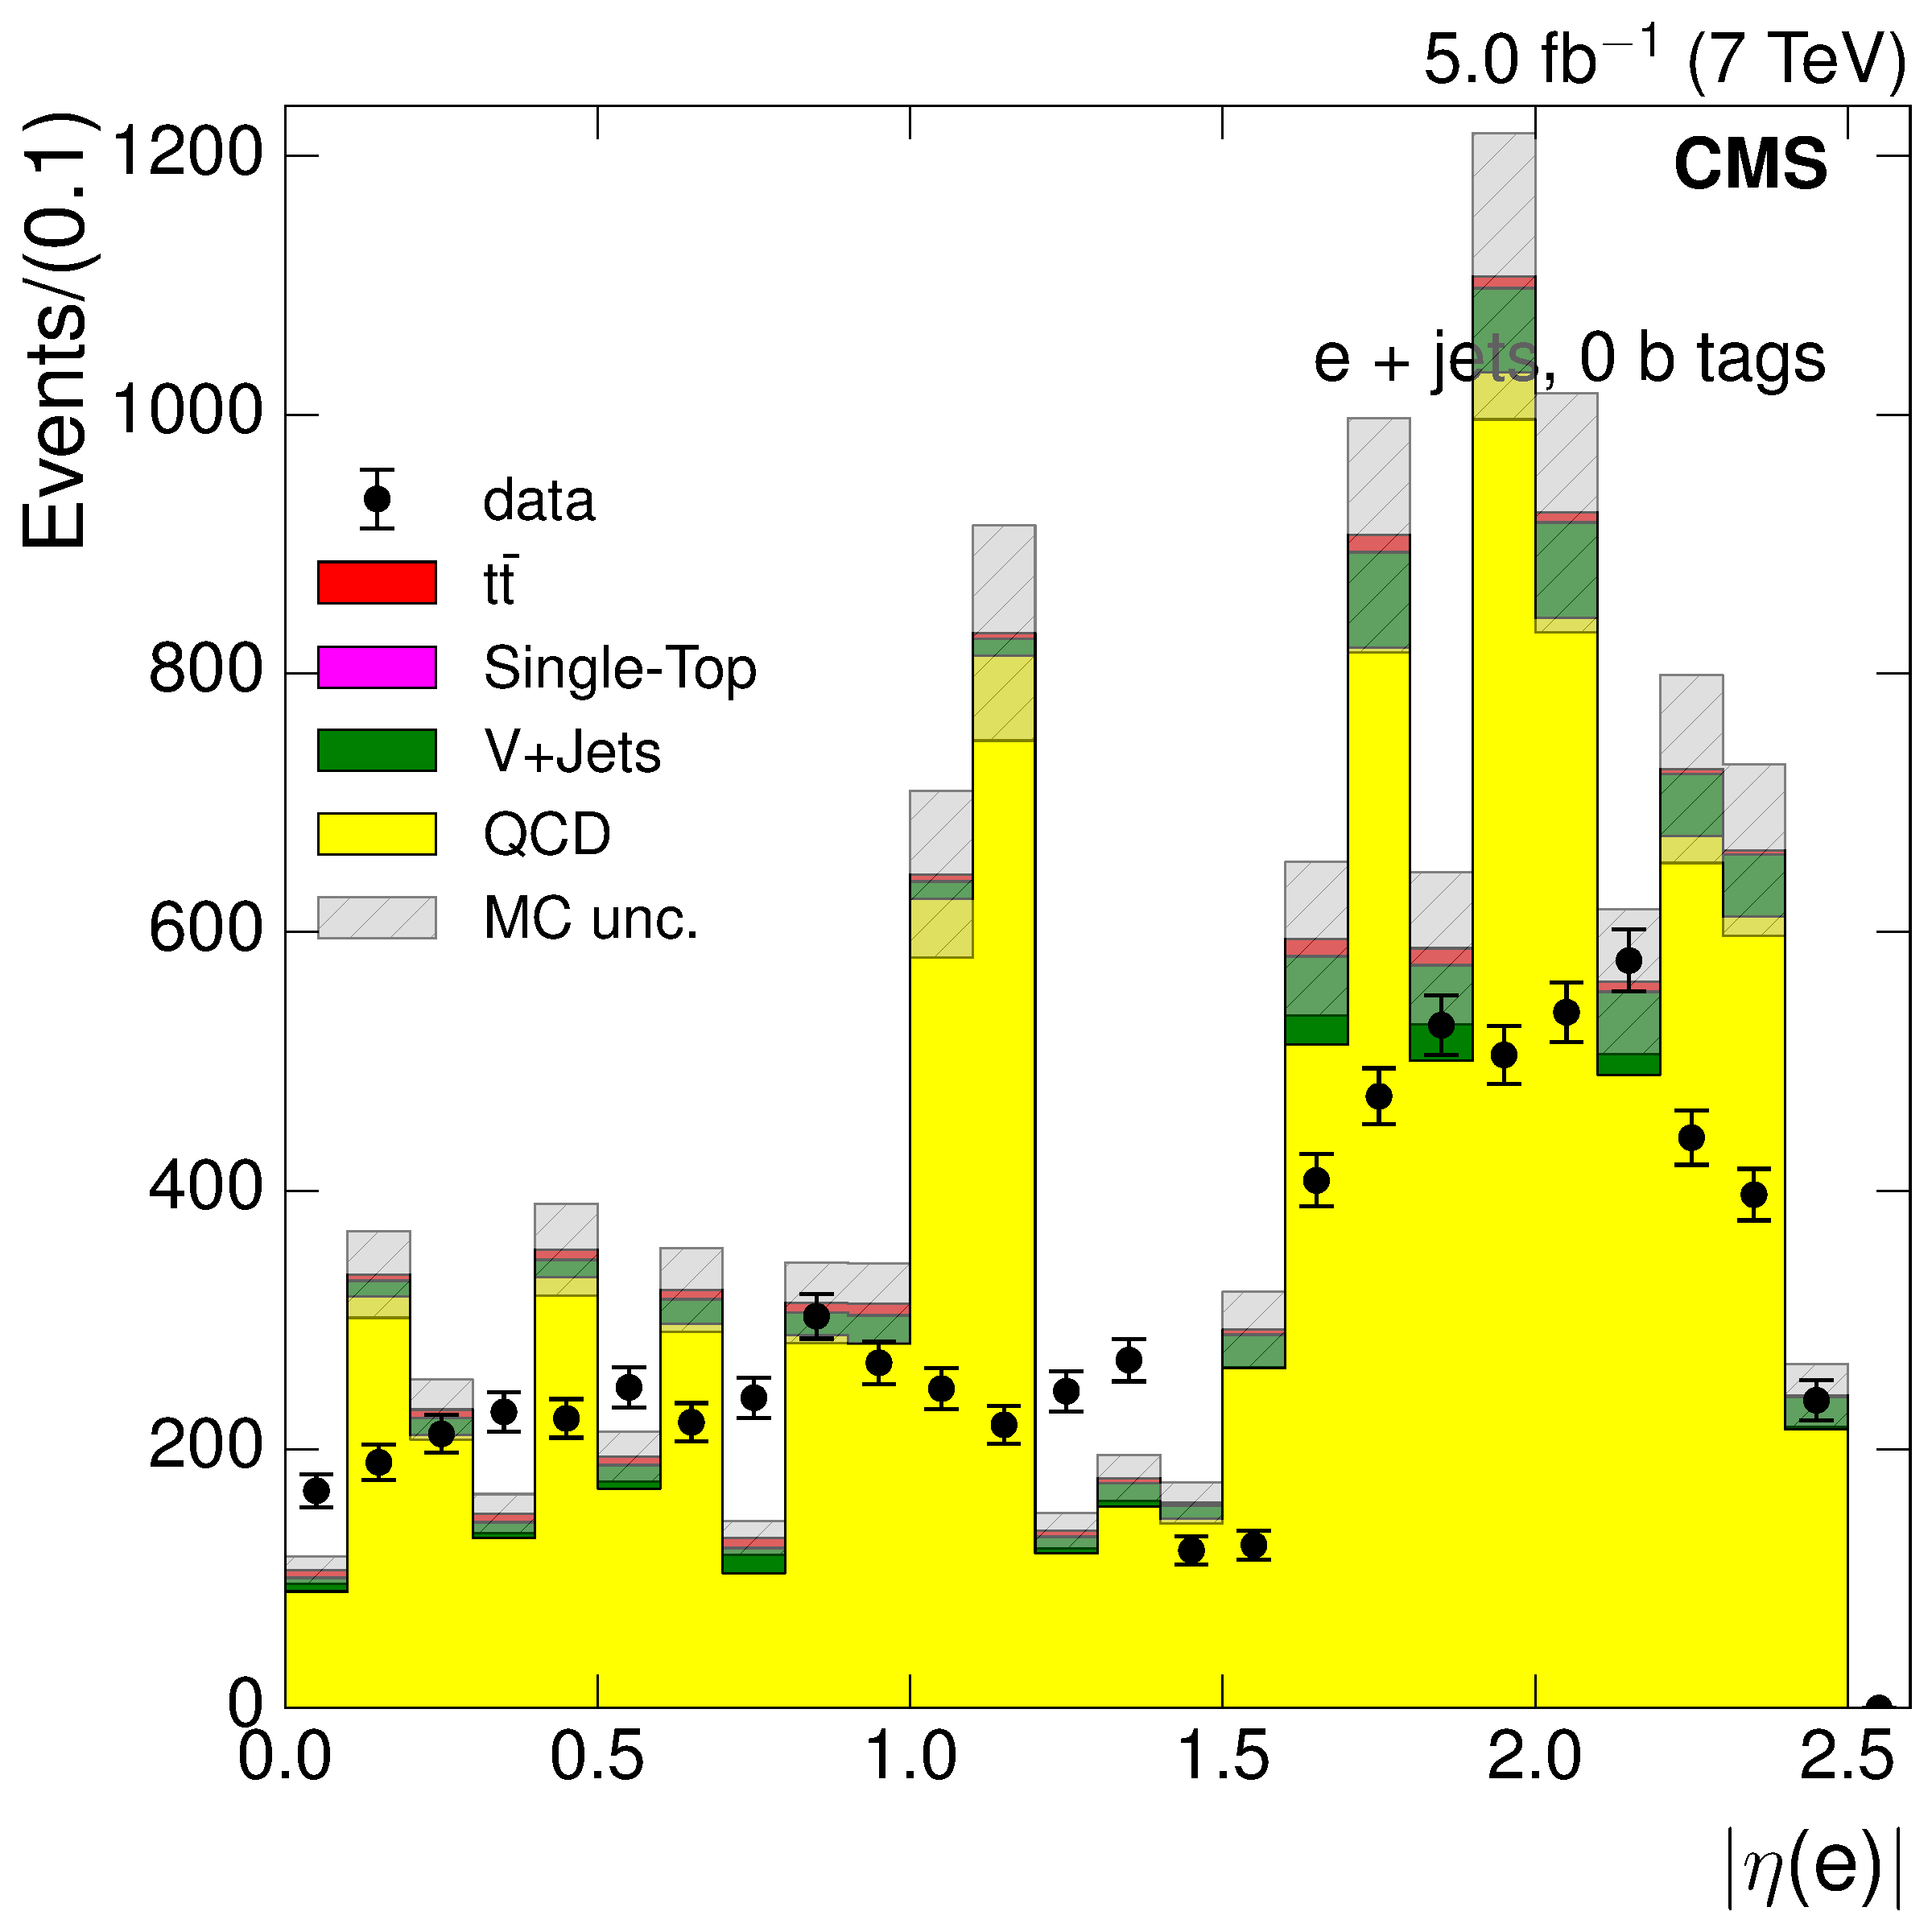
\includegraphics[width=0.45\textwidth]{Chapters/07_08_09_Analysis/Images/control_plots/before_fit/7TeV/qcd_plots/QCD_electron_AbsEta_conversion_control_region_0btag}\hfill
    	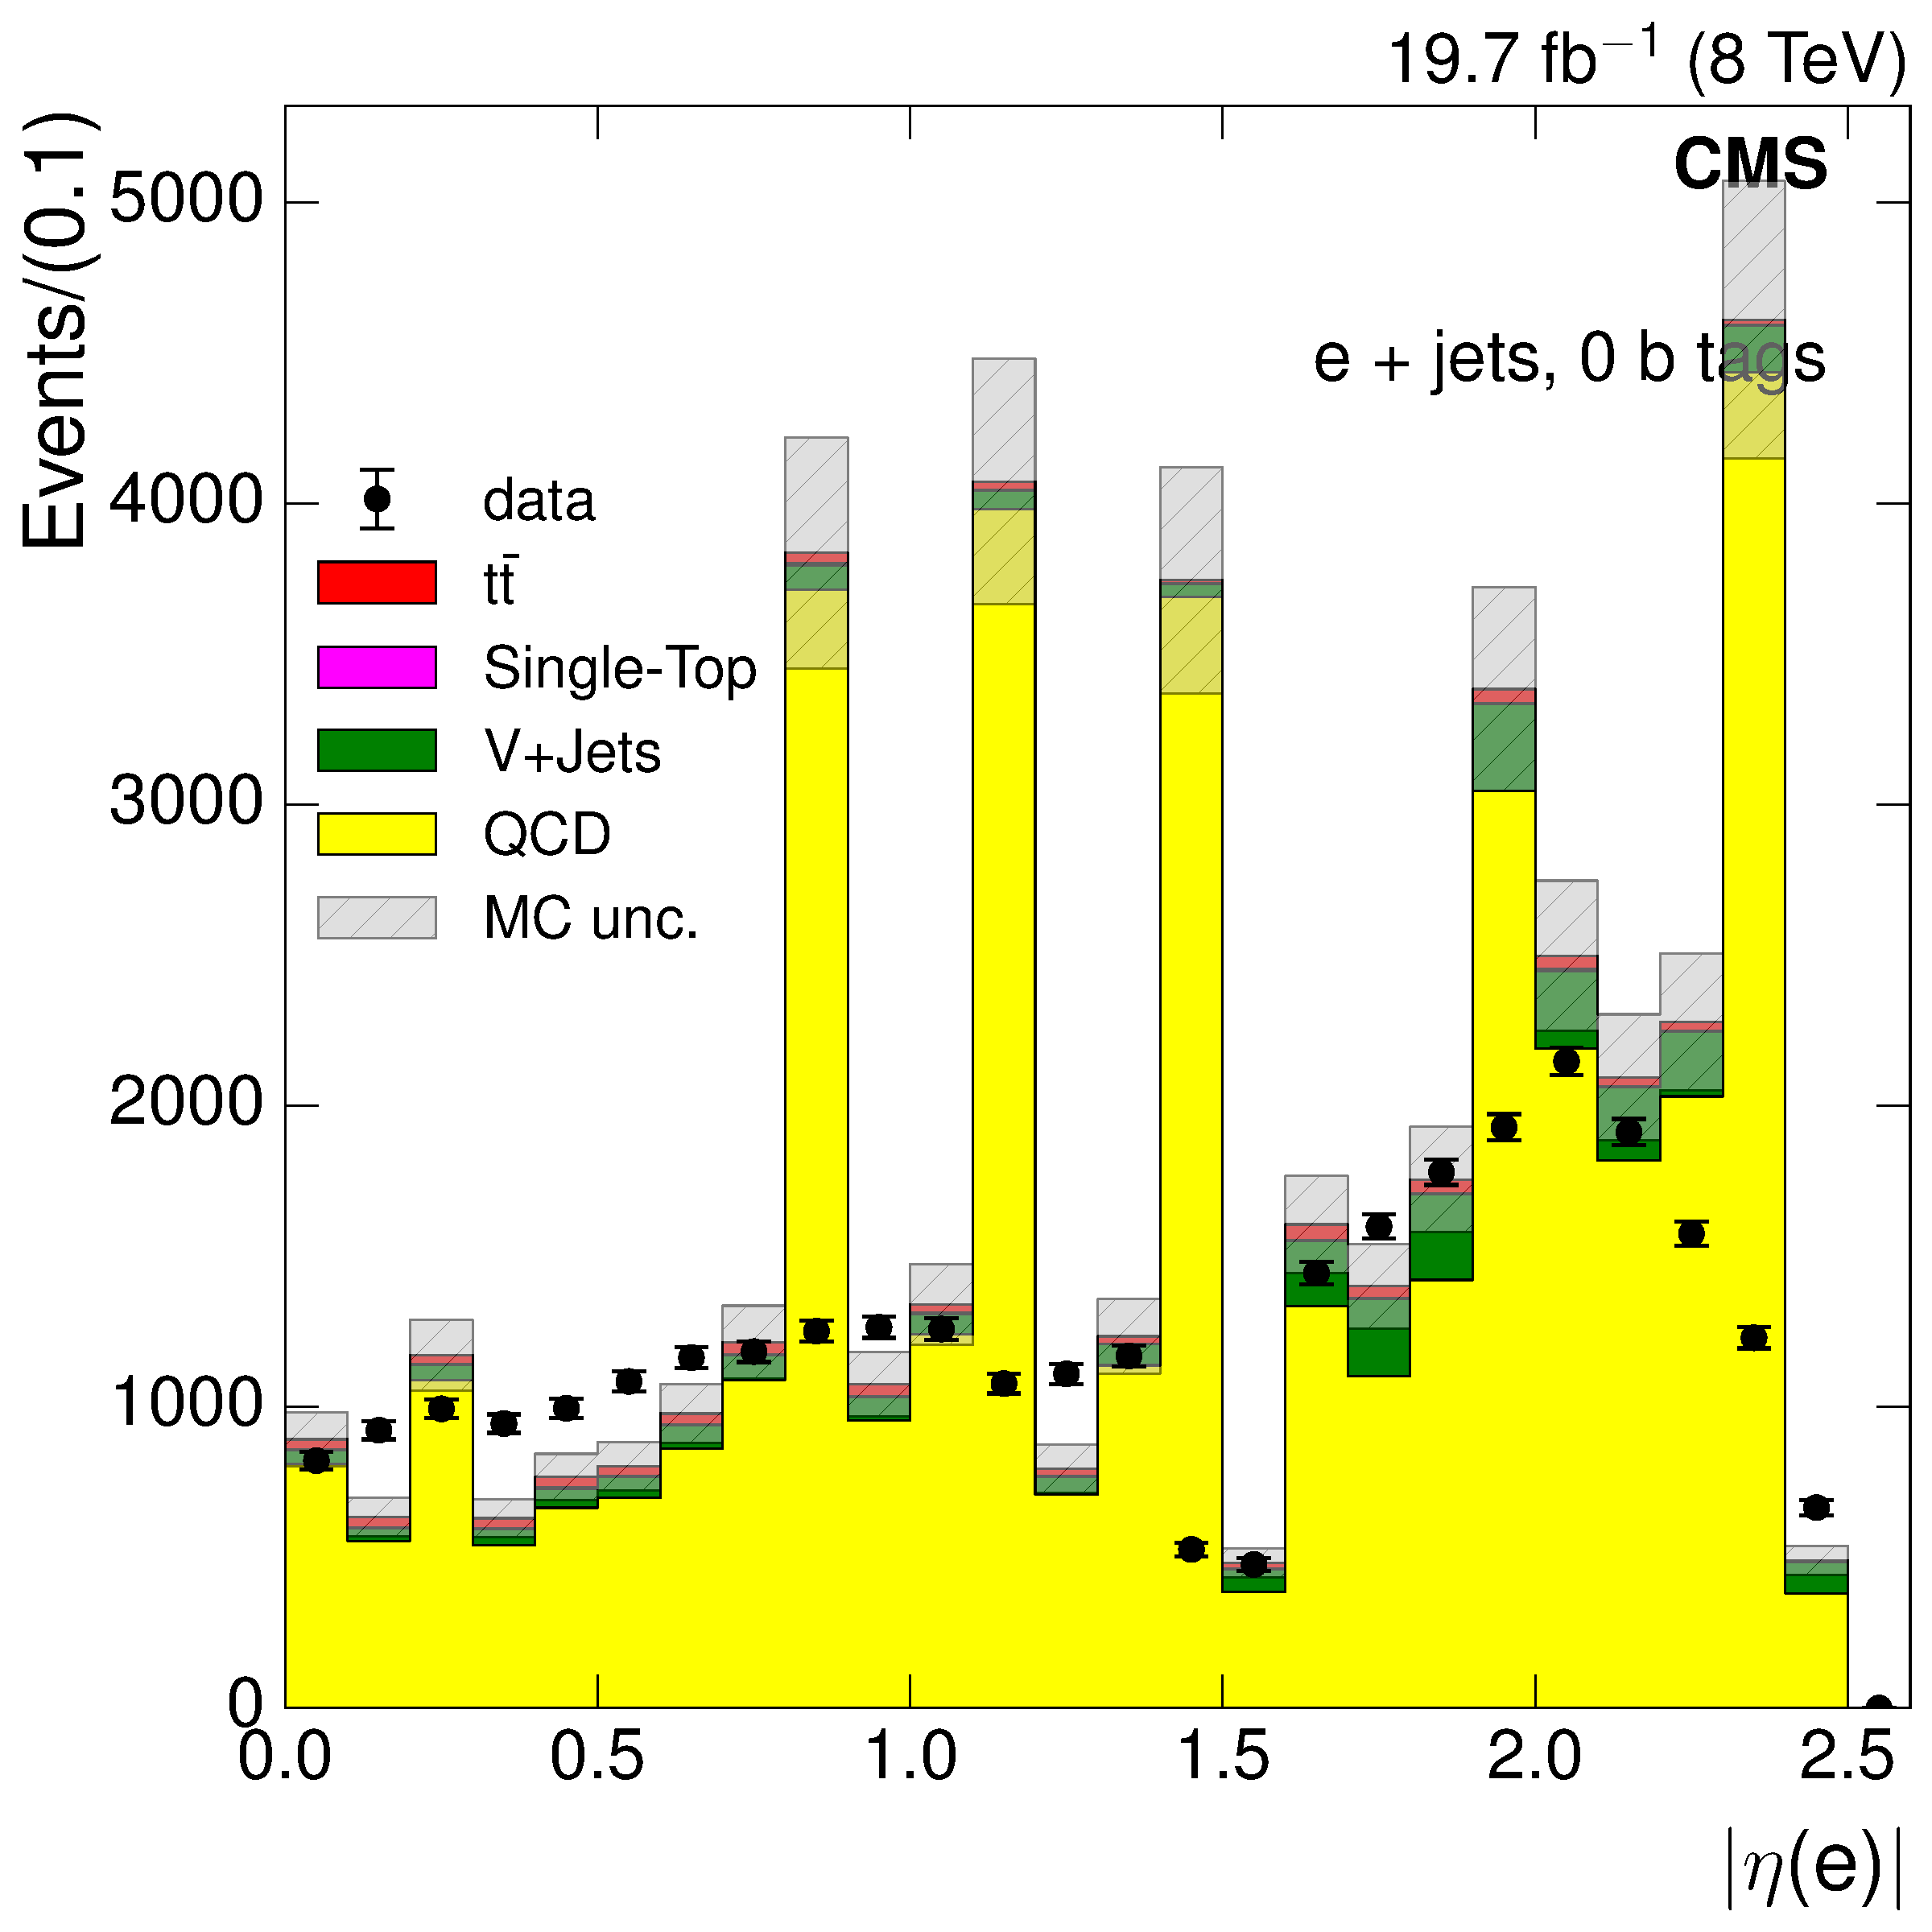
\includegraphics[width=0.45\textwidth]{Chapters/07_08_09_Analysis/Images/control_plots/before_fit/8TeV/qcd_plots/QCD_electron_AbsEta_conversion_control_region_0btag}
	  	\label{subfig:qcd_conversion_region}
	}\\
  	\subfloat[]{
  		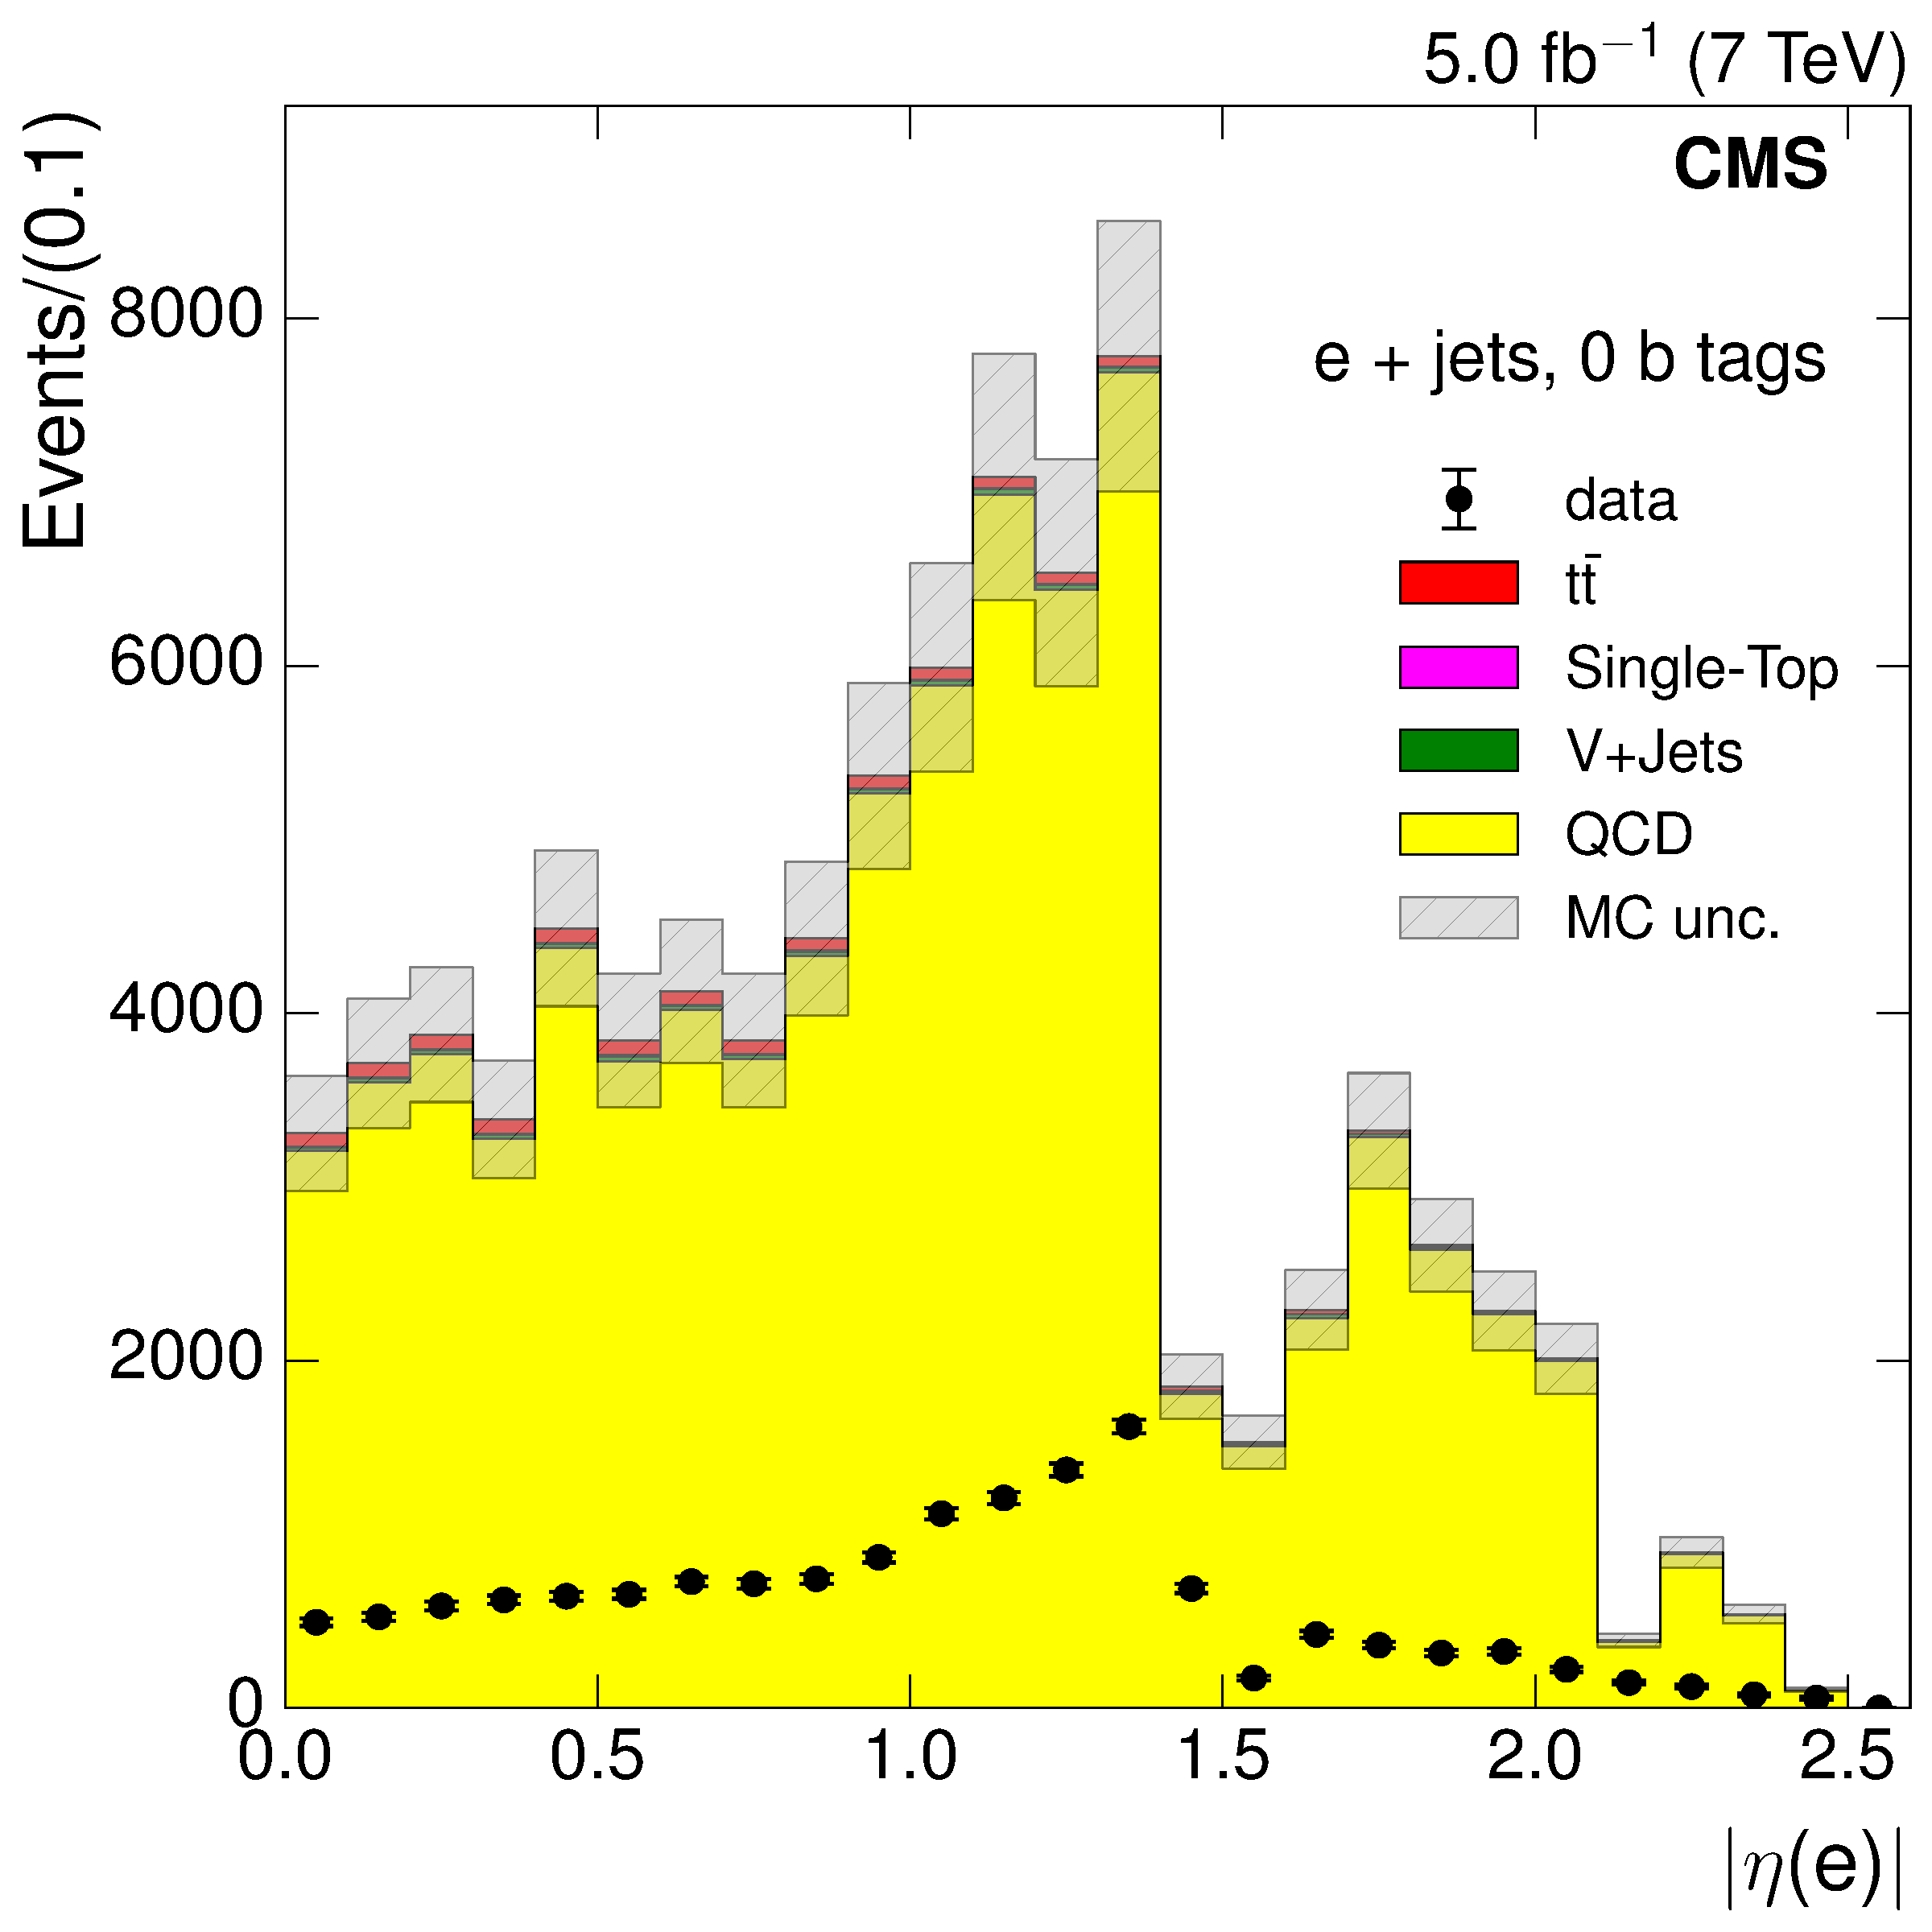
\includegraphics[width=0.45\textwidth]{Chapters/07_08_09_Analysis/Images/control_plots/before_fit/7TeV/qcd_plots/QCD_electron_AbsEta_non_iso_control_region_0btag}\hfill
	  	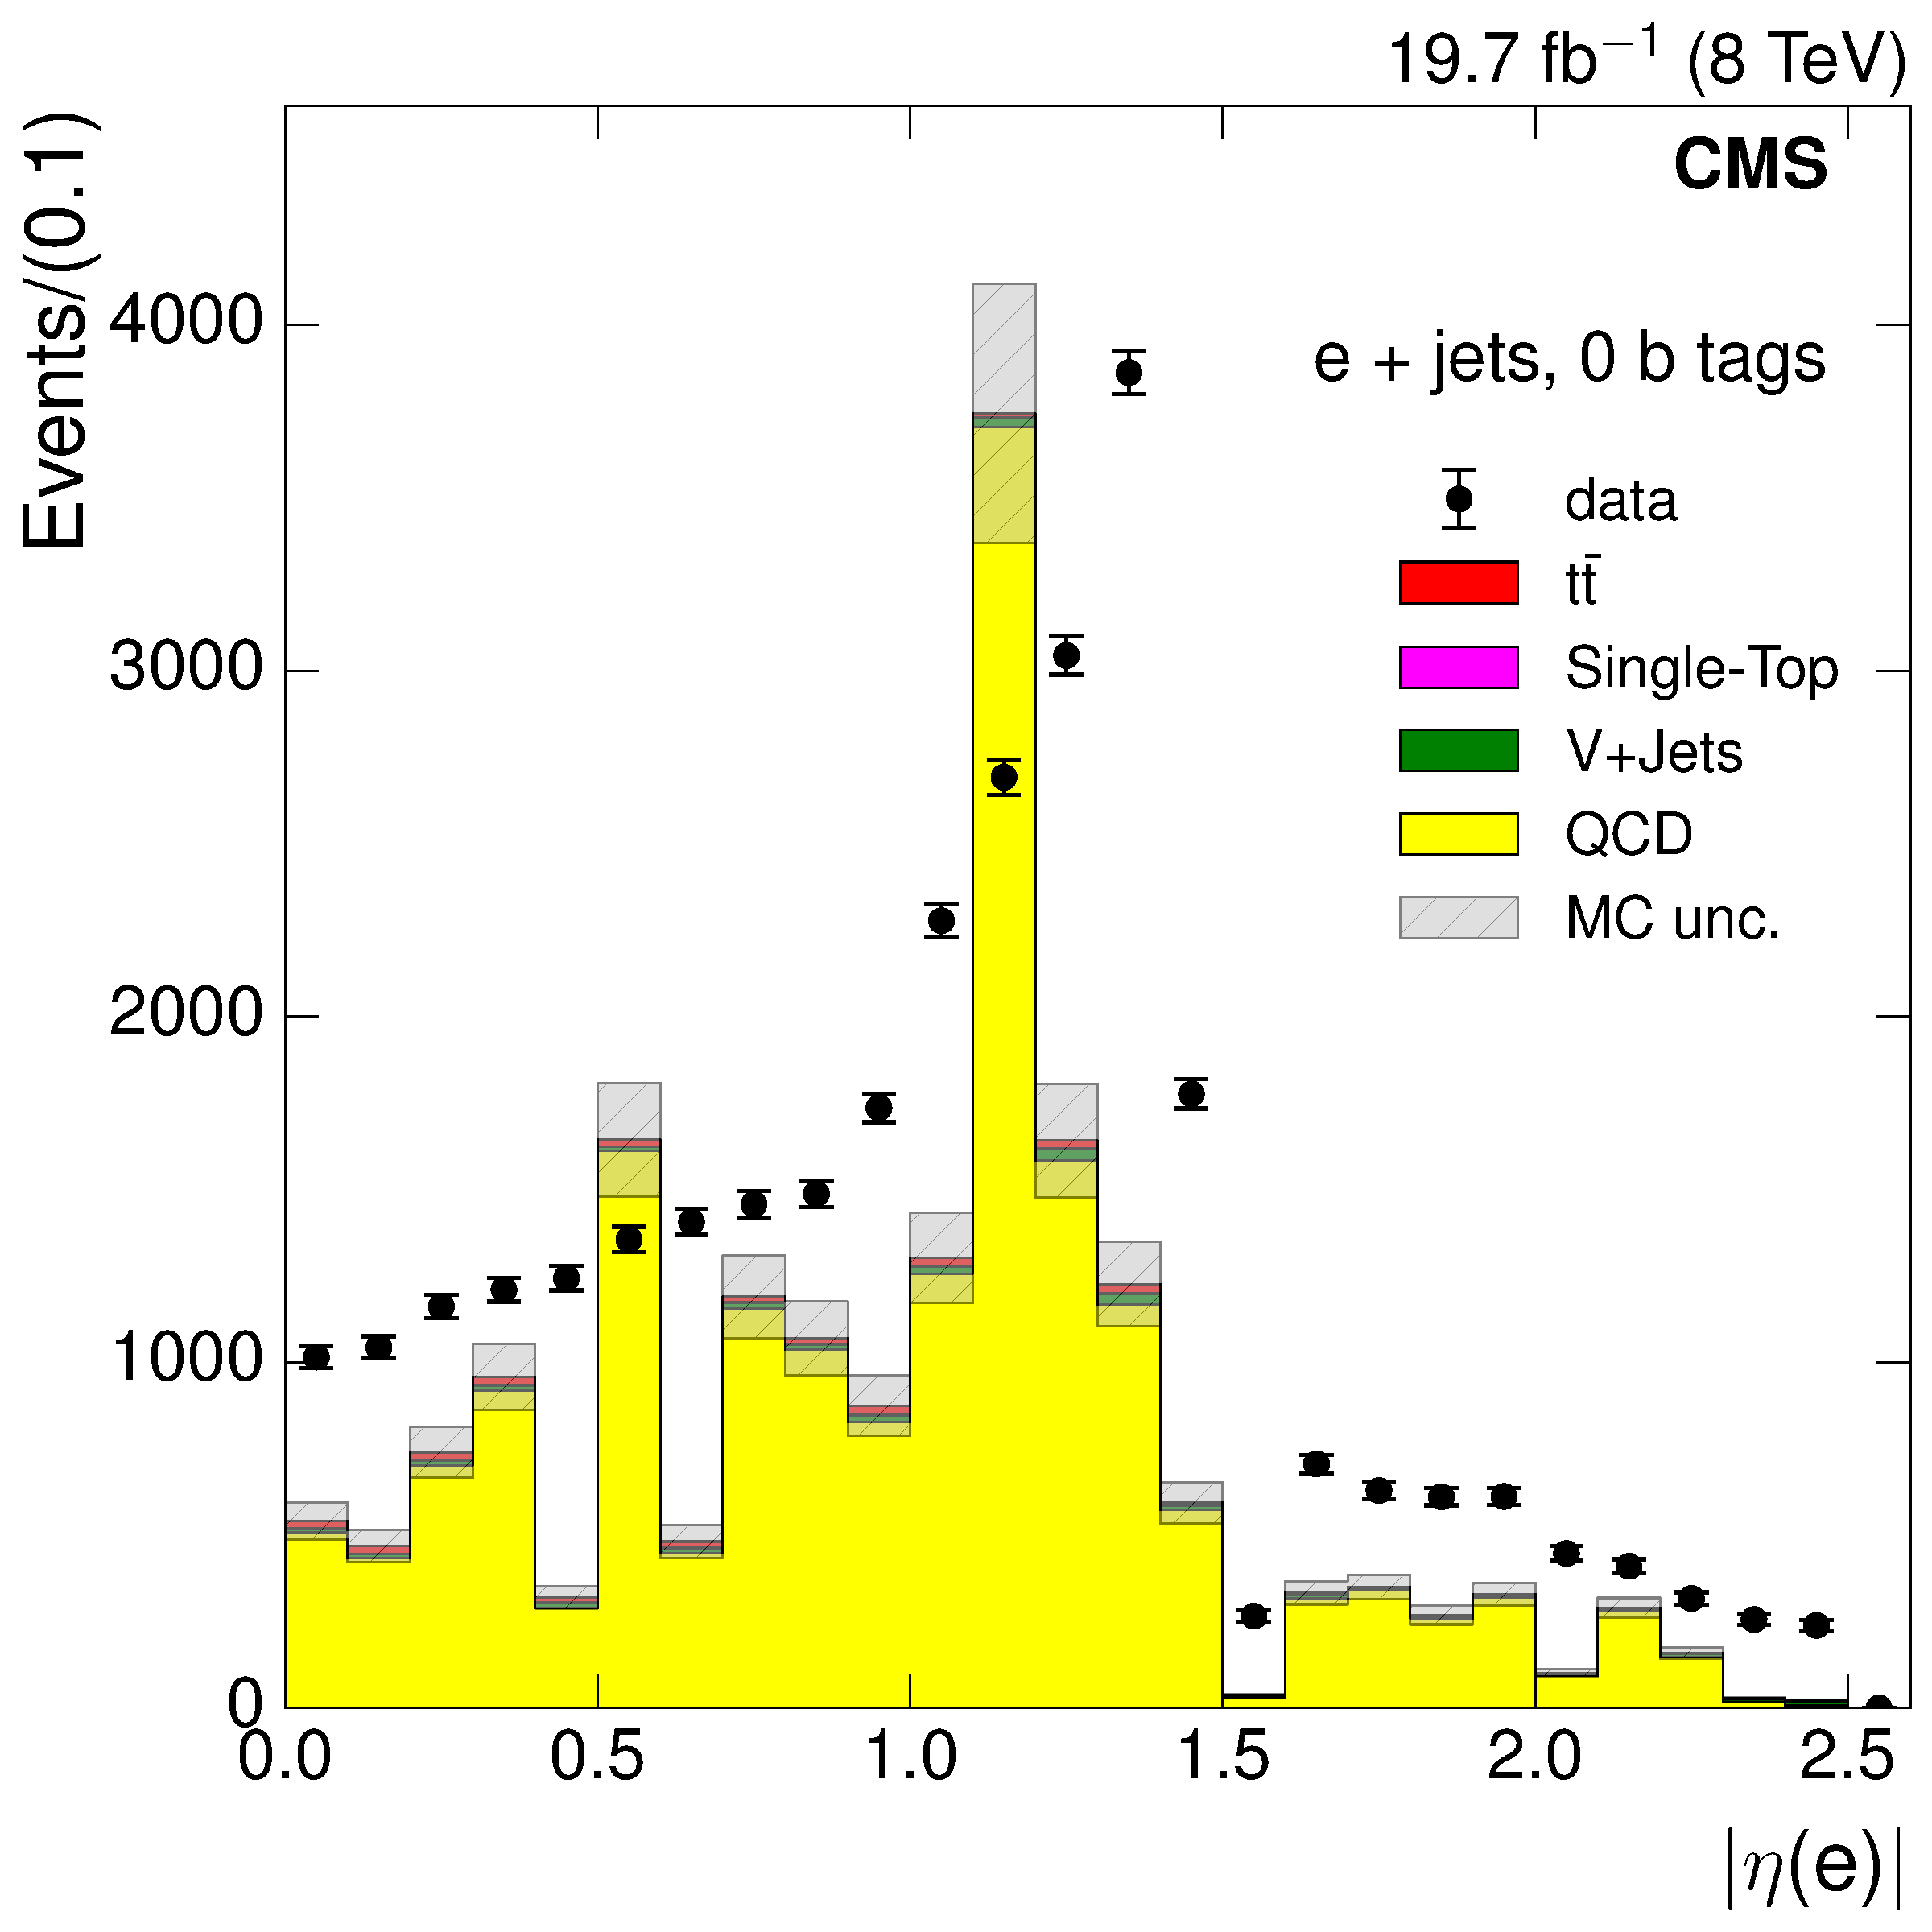
\includegraphics[width=0.45\textwidth]{Chapters/07_08_09_Analysis/Images/control_plots/before_fit/8TeV/qcd_plots/QCD_electron_AbsEta_non_iso_control_region_0btag}
	  	\label{subfig:non-isolated_region}
	}\\
  	\subfloat[]{
  		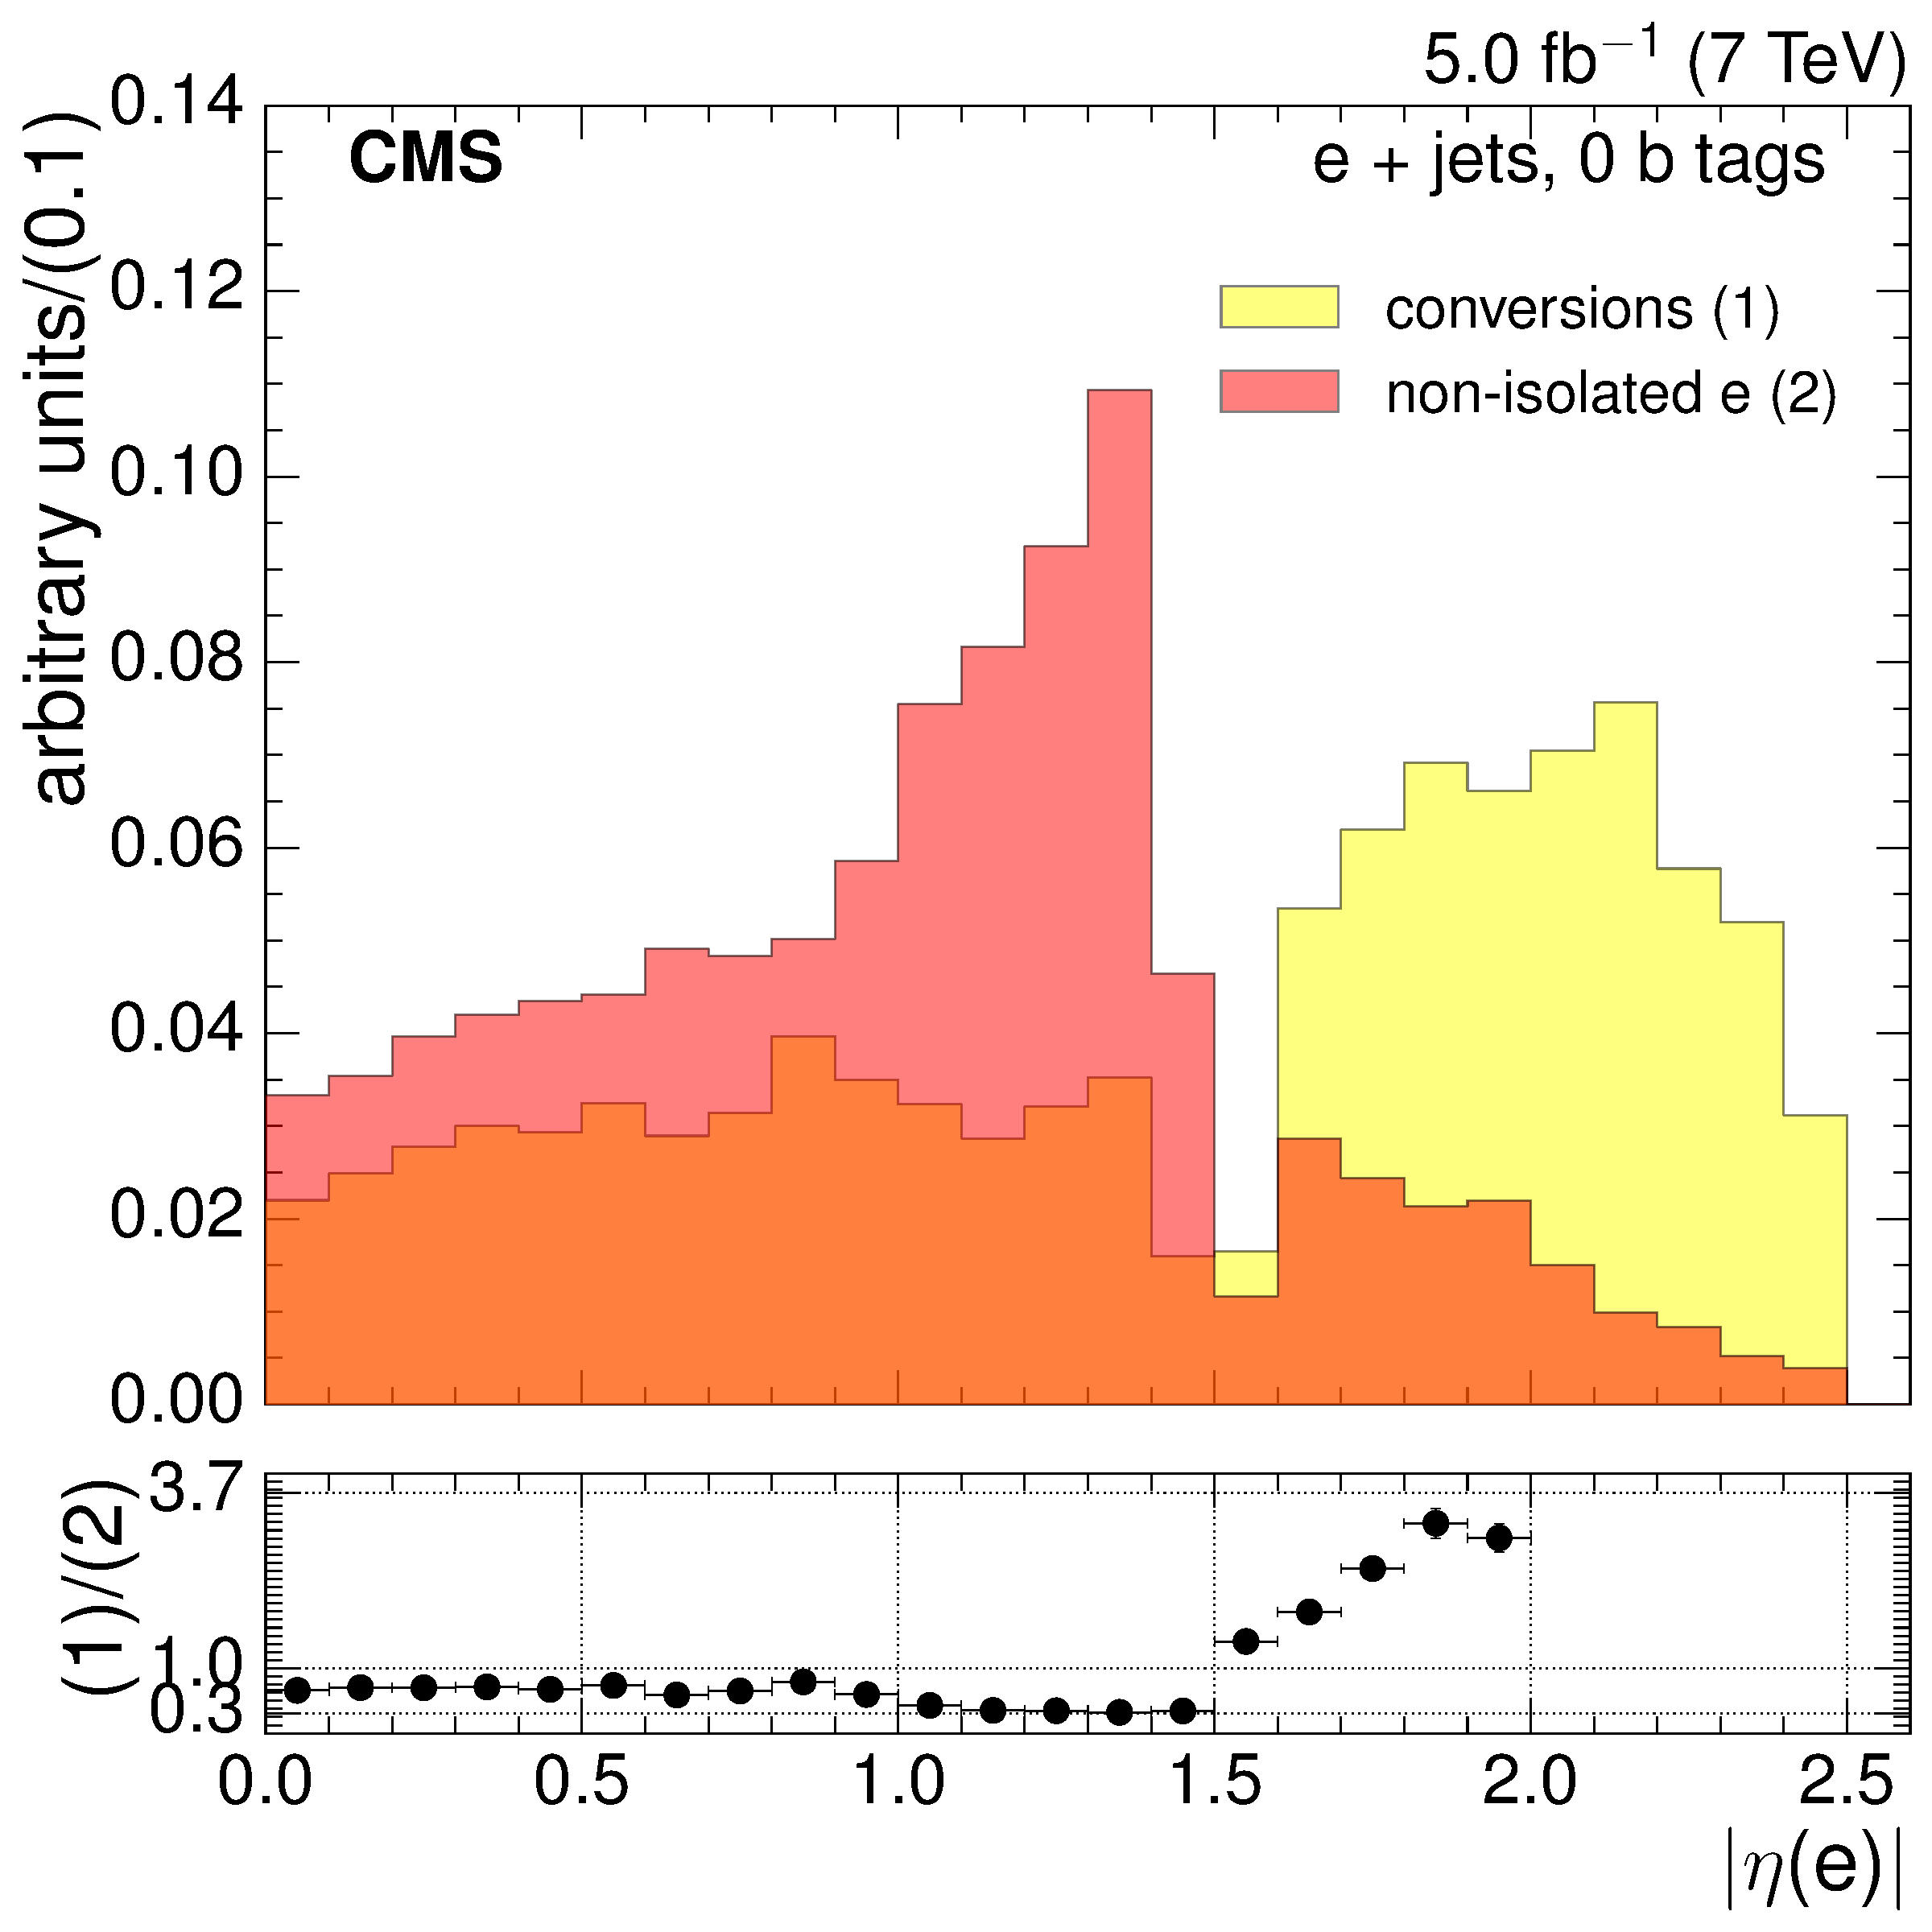
\includegraphics[width=0.45\textwidth]{Chapters/07_08_09_Analysis/Images/control_plots/before_fit/7TeV/qcd_plots/shape_comparisons/QCD_electron_AbsEta_control_region_comparison_0btag}\hfill
	  	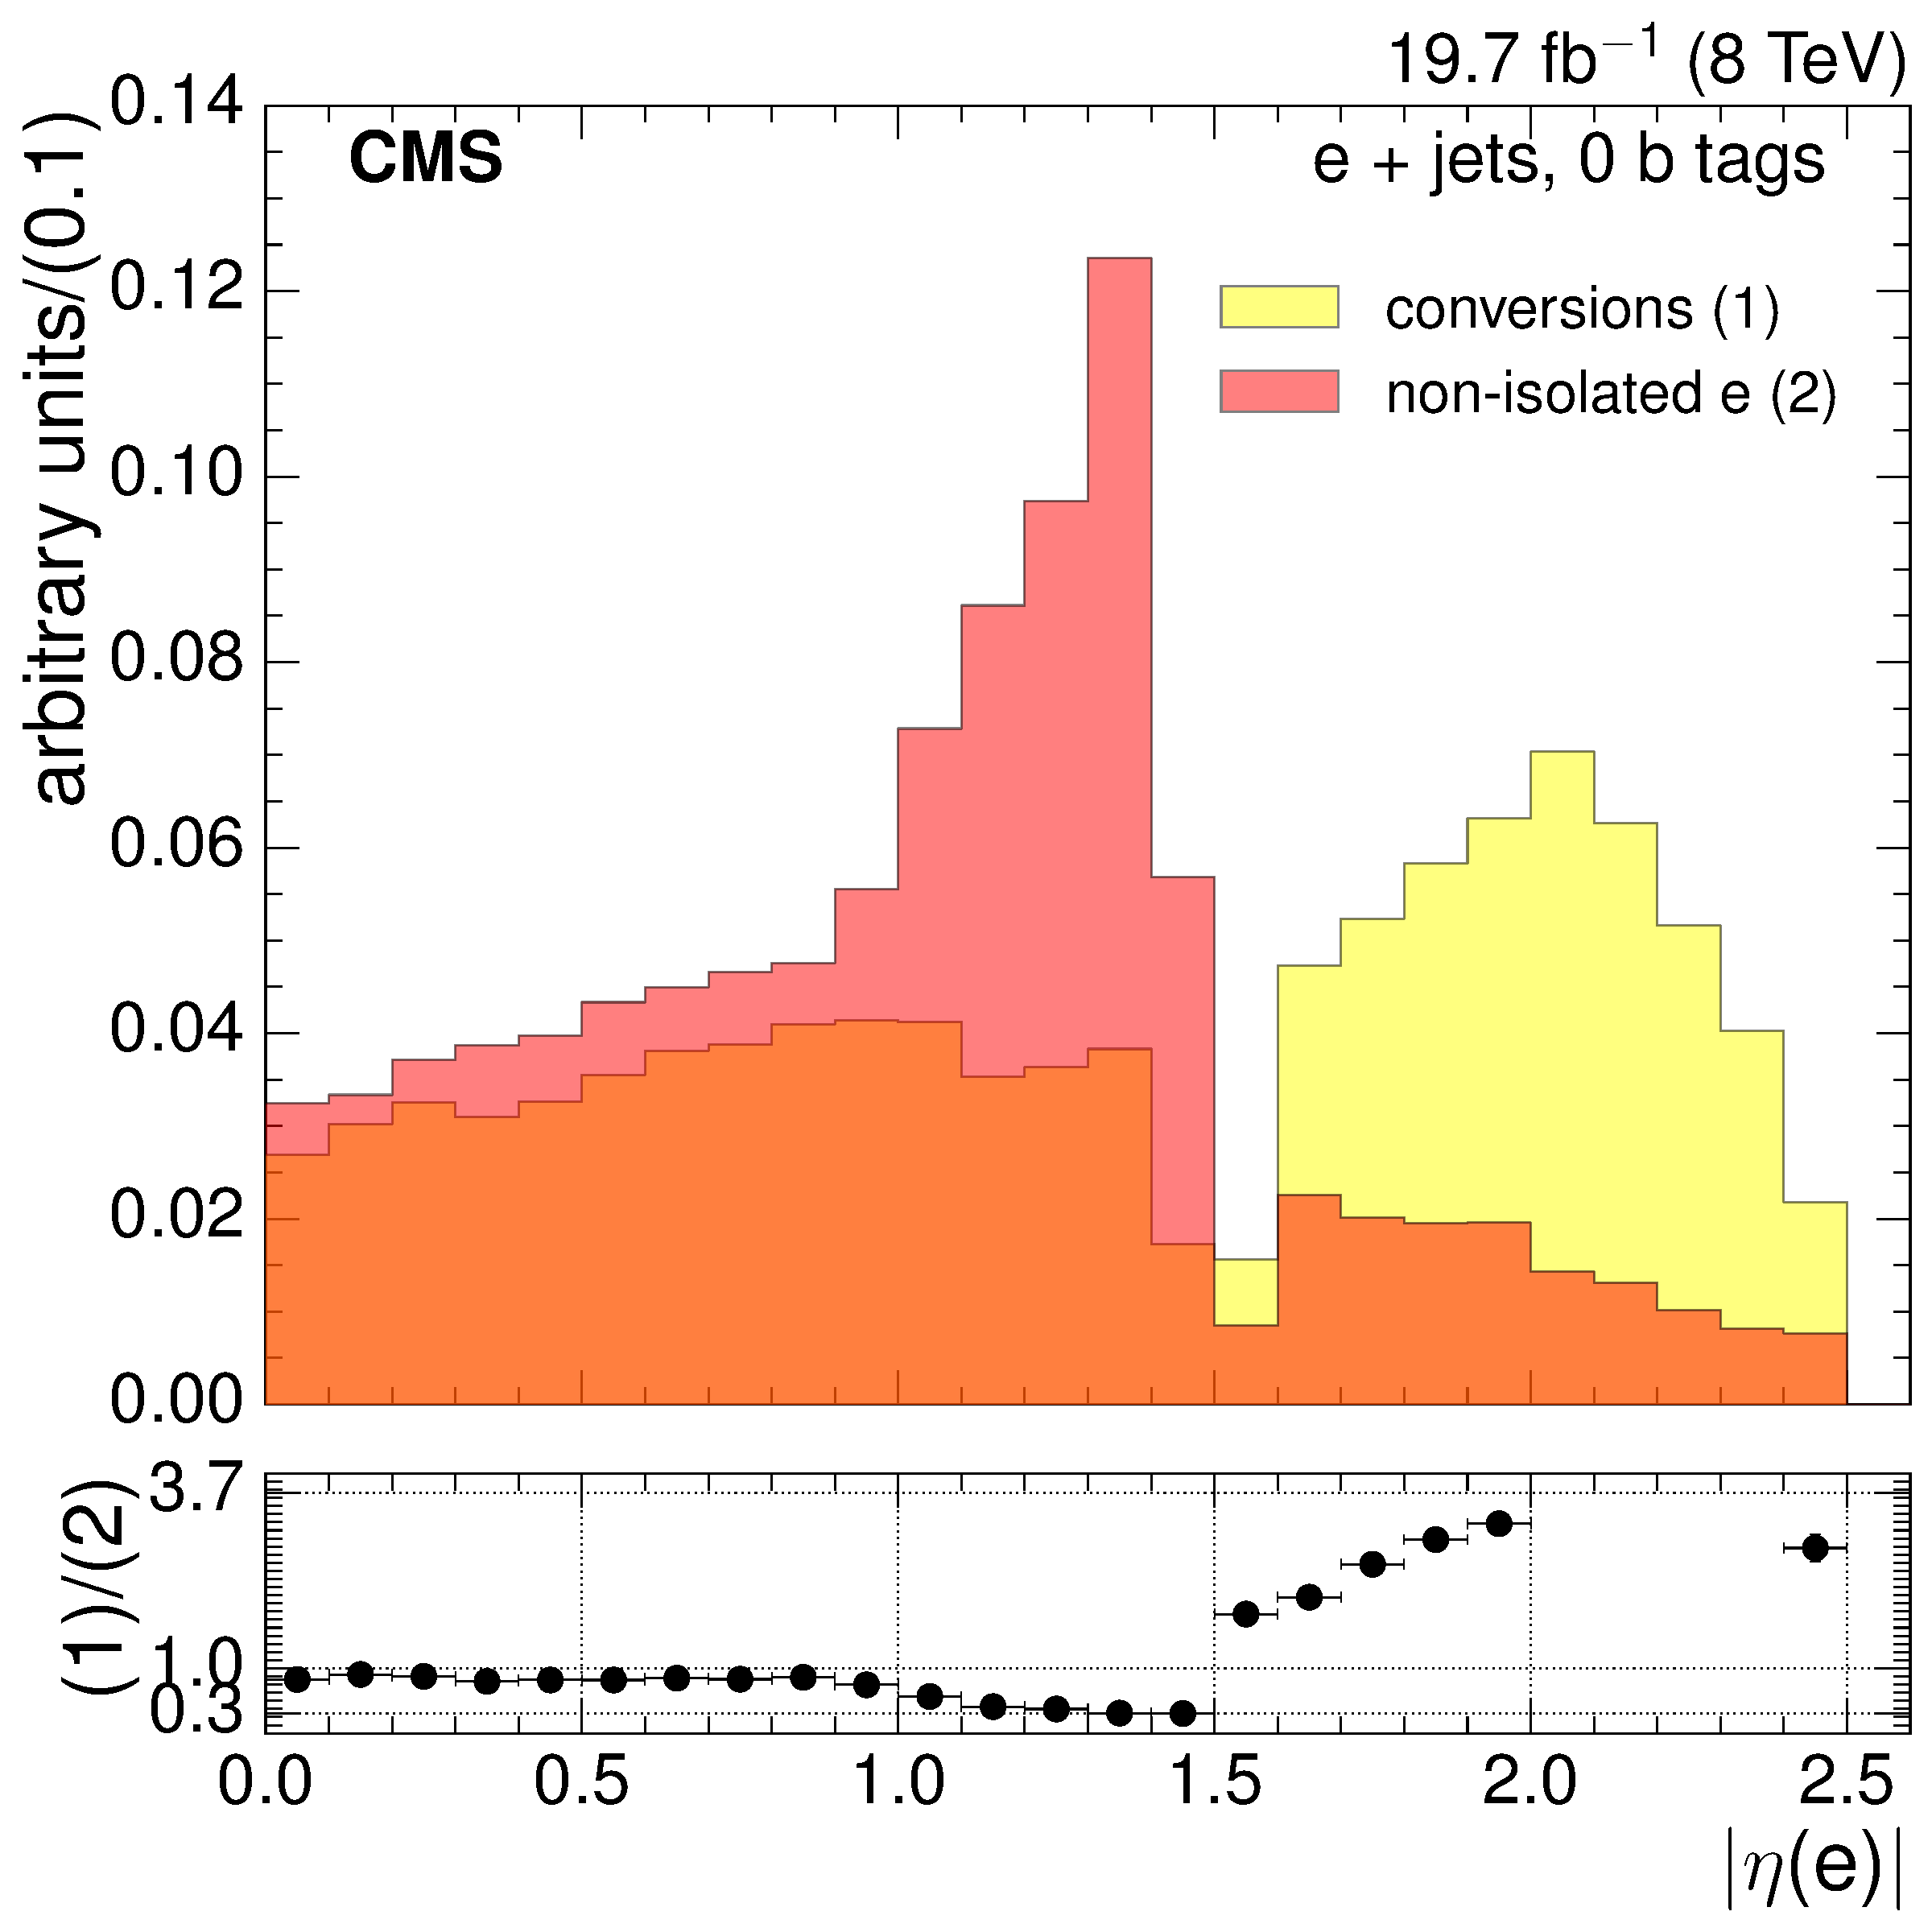
\includegraphics[width=0.45\textwidth]{Chapters/07_08_09_Analysis/Images/control_plots/before_fit/8TeV/qcd_plots/shape_comparisons/QCD_electron_AbsEta_control_region_comparison_0btag}
	  	\label{subfig:control_region_comparison}
	}\\
  	\caption[Comparison of QCD selections in the electron+jets channel at $\roots=7\TeV$ and at
    $\roots=8\TeV$.]{Electron \abseta distributions in QCD selections in the electron+jets channel at
    $\roots=7\TeV$ on the left and at $\roots=8\TeV$ on the right, in the conversion region (a) and in the
    non-isolated region (b). A shape comparison between the two regions in data is shown in (c).}
    \label{fig:electron_QCD}
\end{figure}

In the case of the muon+jets channel, the full selection is applied with the exception of the muon relative
isolation requirement, which is switched from $<0.12$ to $>0.3$. This cut value is chosen in order to largely
remove most background processes and produce a high purity QCD sample, as can be seen from
Figure~\ref{fig:muon_qcd_isolation}. There is a resonable agreement between MC and data here, although again
there are some spikes representing the lack of simluation statistics. As in the electron channel, the \btag
requirement is reduced to 0 \btags and in addition the jet multiplicity requirement is reduced to require at
least three jets, to improve statistics and to ensure a purer QCD sample.

\begin{figure}[hbtp]
    \centering
      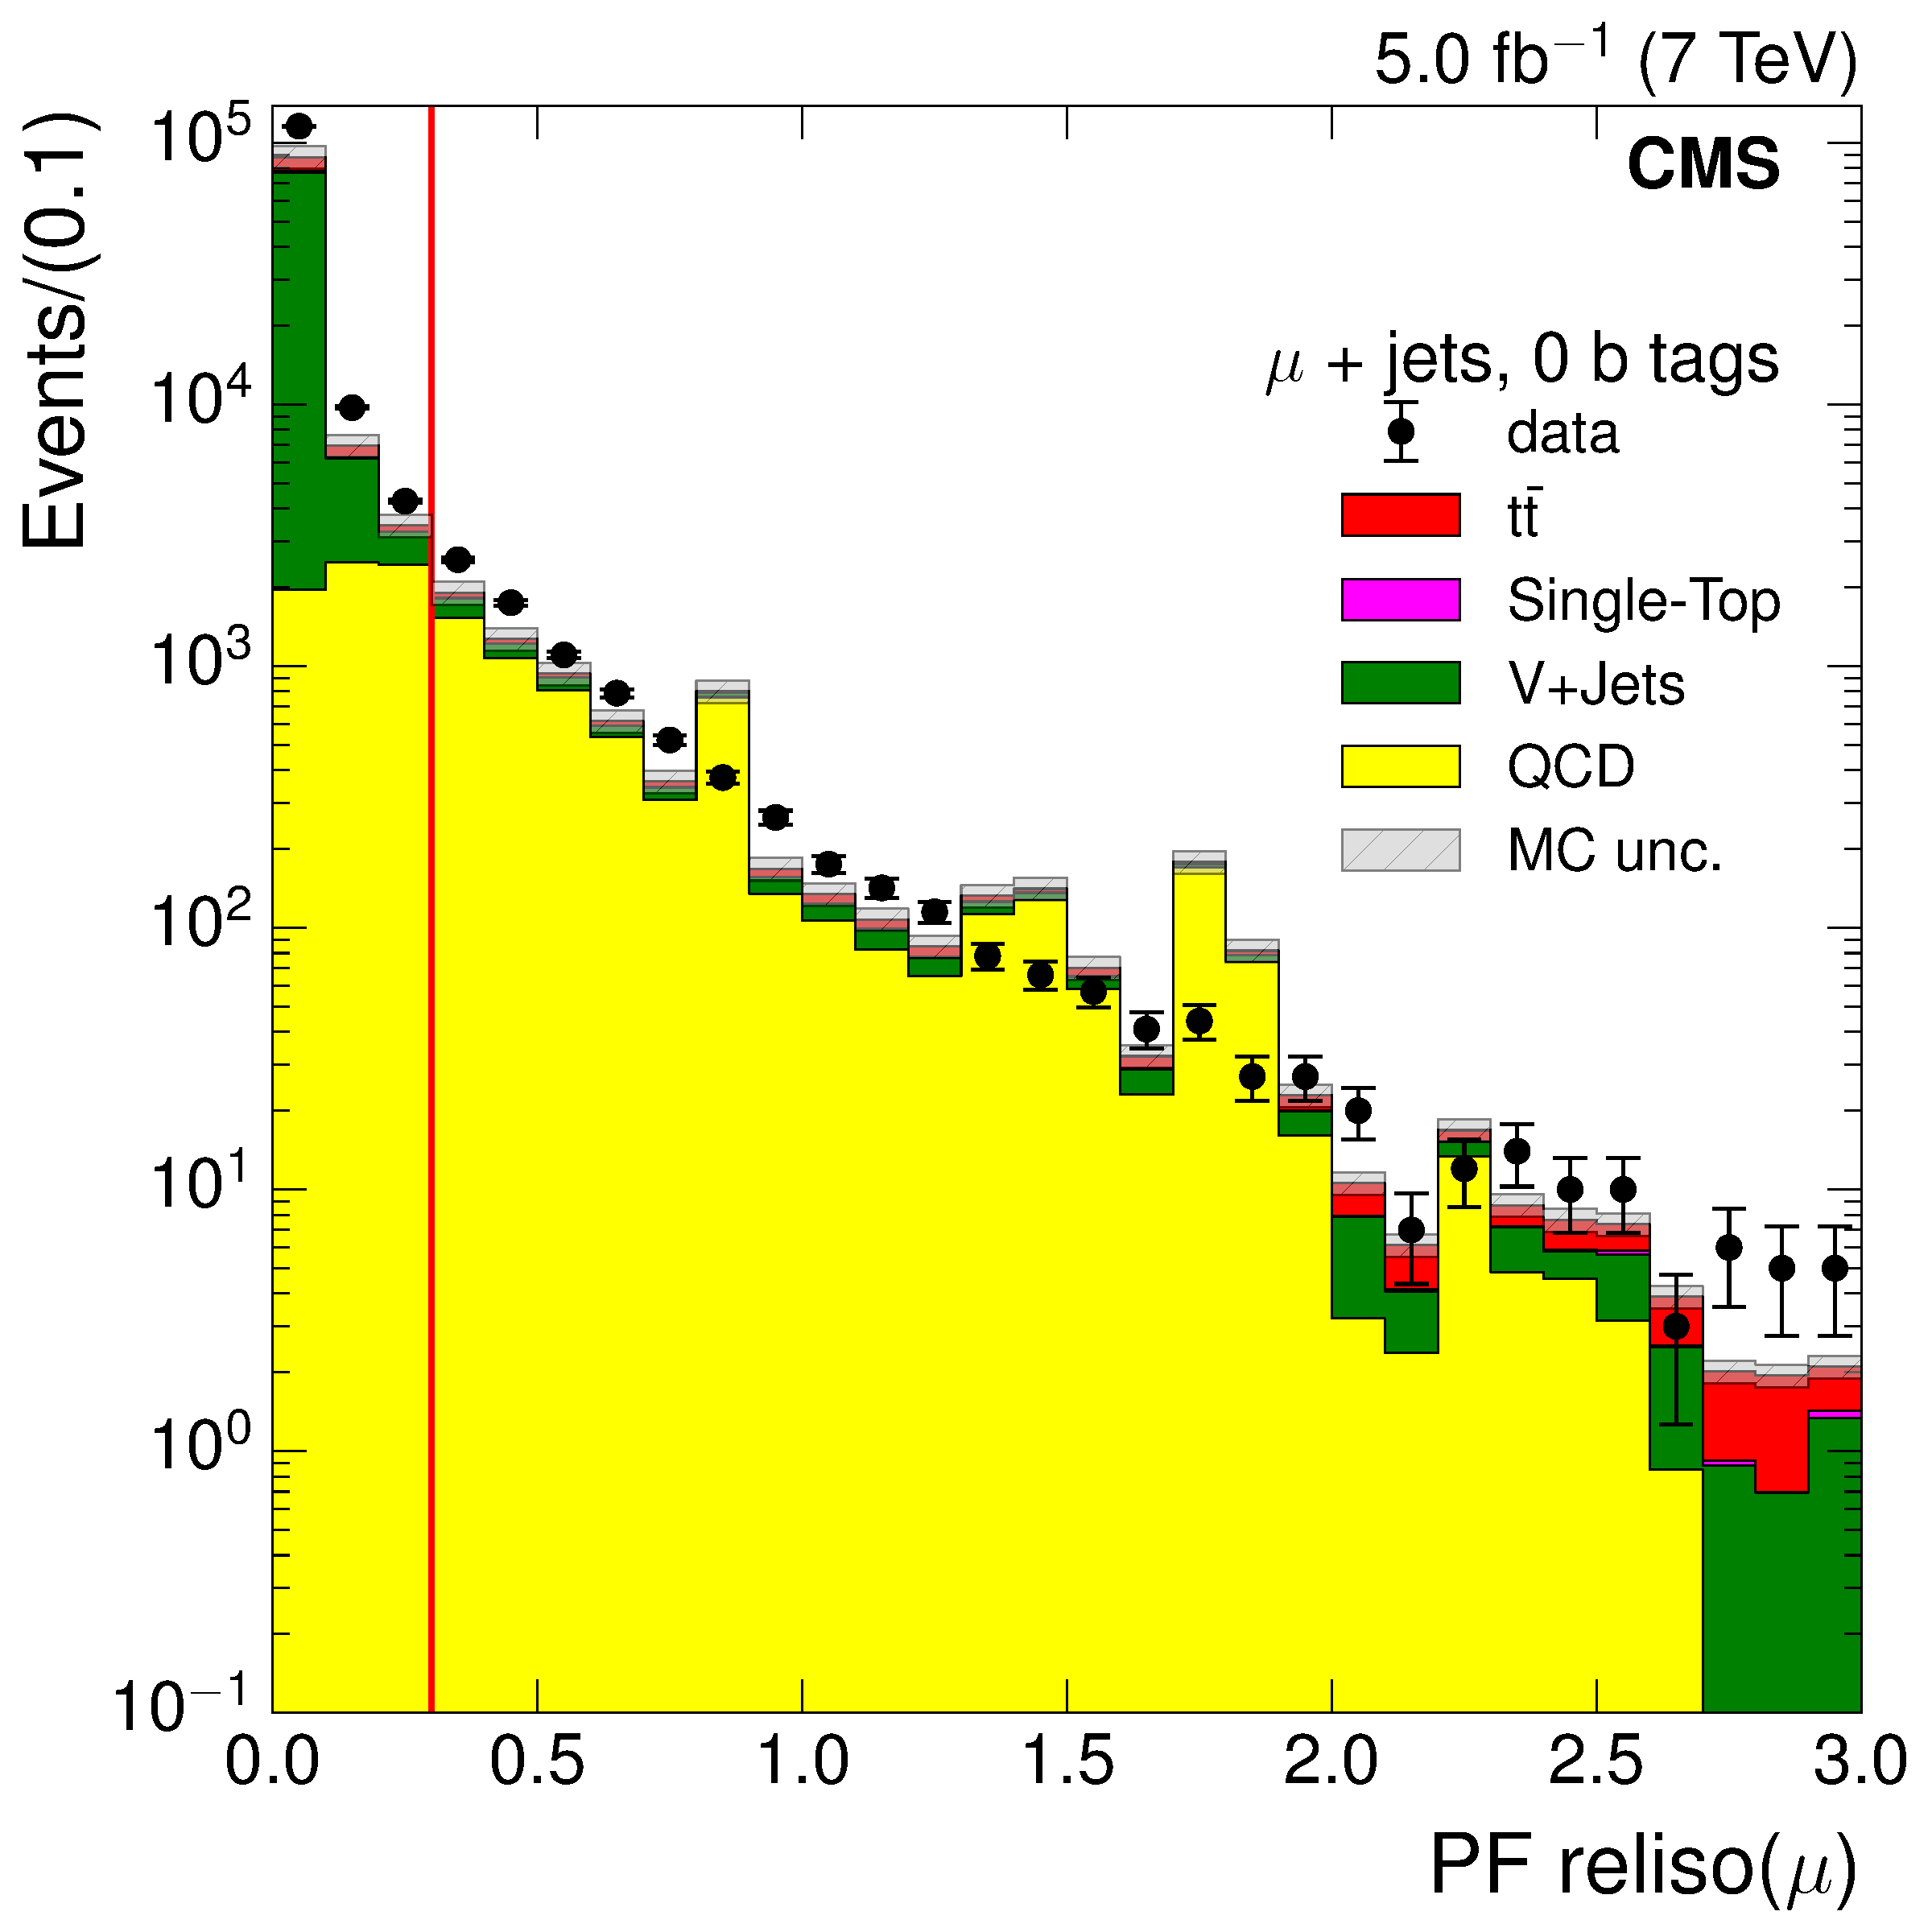
\includegraphics[width=0.48\textwidth]{Chapters/07_08_09_Analysis/Images/control_plots/before_fit/7TeV/qcd_plots/QCD_muon_pfIsolation_with_cutline_0btag}\hfill
      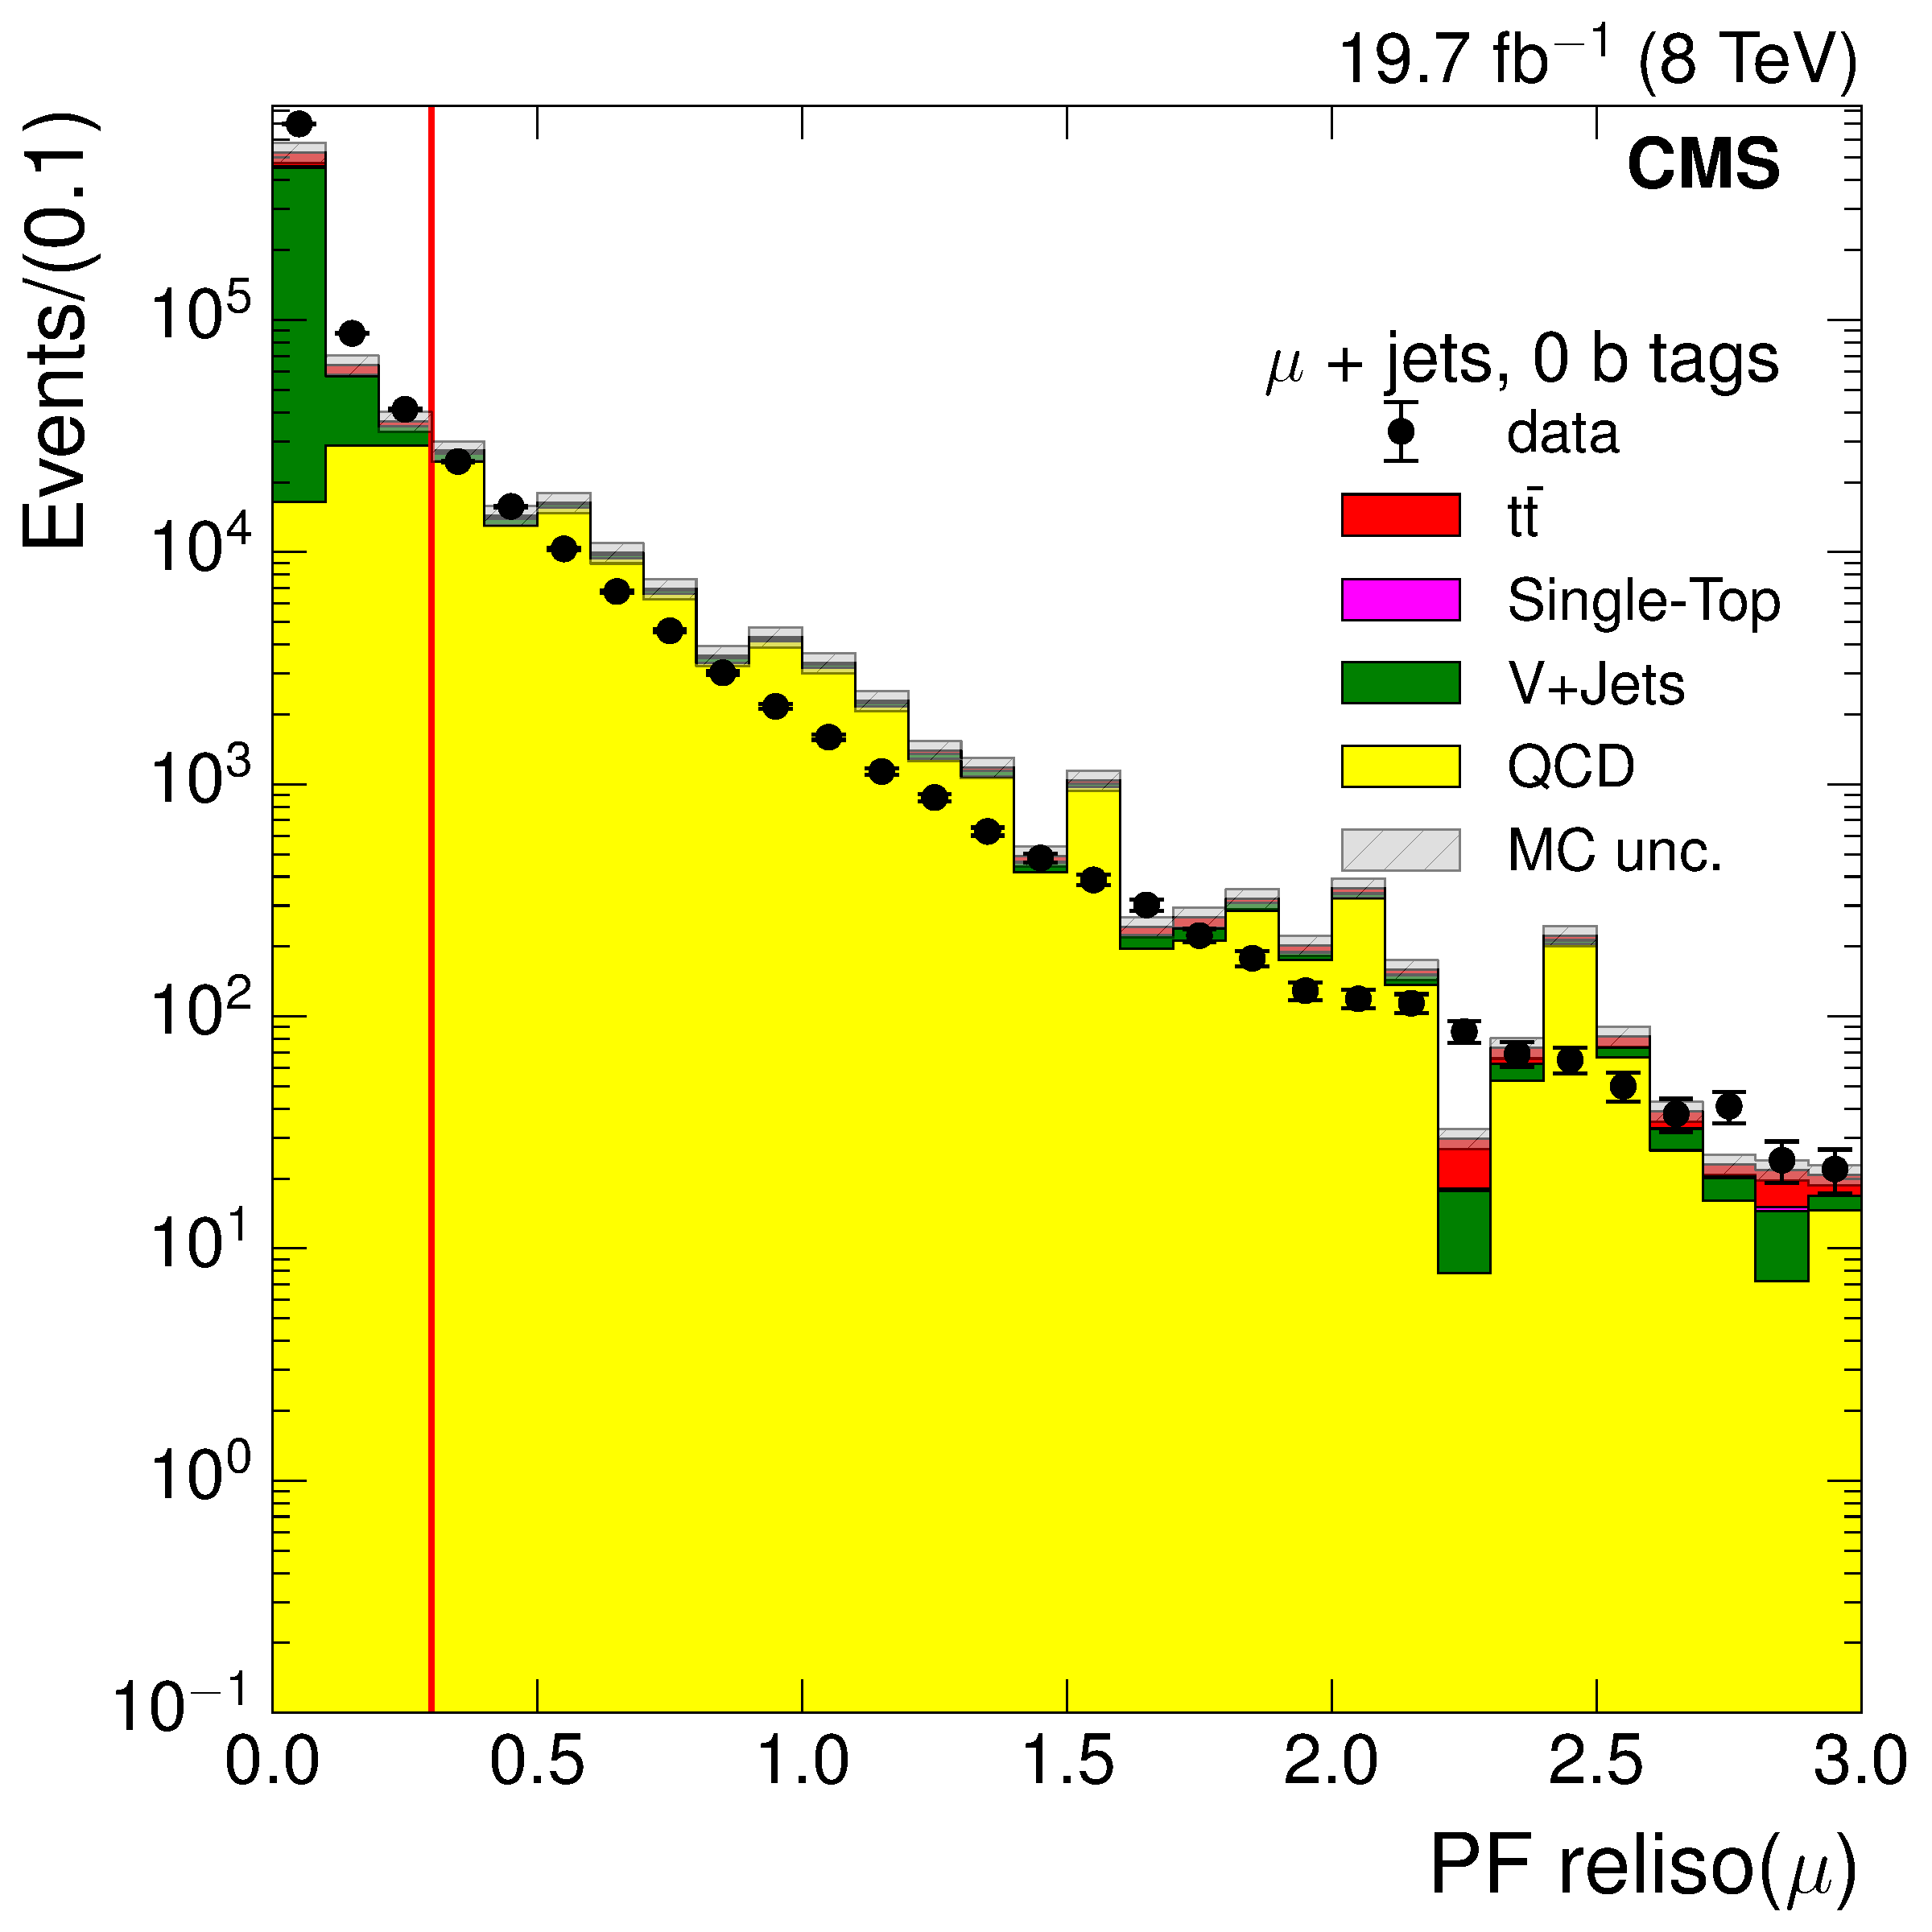
\includegraphics[width=0.48\textwidth]{Chapters/07_08_09_Analysis/Images/control_plots/before_fit/8TeV/qcd_plots/QCD_muon_pfIsolation_with_cutline_0btag}\\
      \caption[PF relative isolation distributions in the muon+jets channel at $\roots=7\TeV$ and
      $\roots=8\TeV$]{PF relative isolation distributions in the muon+jets channel, before subtraction of
      \ttbar, single top and \VpJets at $\roots=7\TeV$ (left) and $\roots=8\TeV$ (right).}
     \label{fig:muon_qcd_isolation}
\end{figure}

Relative to other processes, QCD events are computationally extremely expensive to produce in simulation,
owing to their large cross section requiring high numbers of events. Neverthless, the number of events passing
the selection will be very small compared to the number of events passing the signal selection, even with
simulated samples with high statistics, meaning there is limited value in obtaining additional statistics
for QCD samples. Since the number of events passing the QCD background selections is relatively low, the
effect of even large uncertainties in the QCD background on the total number of events will be minimal.

Due to the low statistics of the QCD samples obtained from data, the inclusive QCD shape over all bins is used
in every bin for each primary variable (meaning the shape is obtained over the full range of the primary
variables, rather splitting into bins). The remaining contribution from \ttbar, single-top and \W/\ZpJets
processes is subtracted from the data sample using the estimation from Monte Carlo simulation. The resulting
template of QCD events from data is then used later in the fitting procedure, in place of the equivalent Monte
Carlo template (Section~\ref{ss:data-mc_comparison}).

\section{Data-MC scale factors}
\label{s:data_mc_scale_factors}
The following sections describe the small but significant discrepancies that exist between data and simulation
regarding pileup modelling~\ref{ss:pileup}; \btagging~\ref{ss:b_tagging}; trigger, identification and
isolation efficiency~\ref{ss:trigger_ID_isolation_corrections}; jet energy scale and jet energy
resolution~\ref{sss:jet_energy_scale}; and \met calculation~\ref{ss:met_corrections}. Scale factors and
corrections are applied to both MC and data to account for these differences. The data-MC scale factors used
are in accordance with the CMS TOP PAG, and the relevant corrections are implemented for 7\TeV and 8\TeV.

\subsection{Pileup}
\label{ss:pileup}
Monte Carlo simulation events are produced by first creating the hard proton-proton interaction of interest in
a proton bunch crossing, and then introducing the additional interactions, pileup. The pileup distribution in
simulation does not reflect the true distribution in data, therefore pileup reweighting is carried out. The
estimation of the pileup distribution in data is obtained using the total inelastic proton-proton cross
section and the instantaneous luminosity measured in each proton bunch crossing, with a tool provided by the
CMS Physics Validation Group. For each number of pileup interactions in simulation, a weight is then produced
to match the respective distribution in data.

There is an uncertainty on the measured luminosity which is currently 2.6~\% for 2012 data~\cite{CMS:2013gfa}
and 2.2~\% for 2011 data~\cite{CMS:2012eui}. The total inelastic cross section has been reported using CMS
forward calorimetry~\cite{Chatrchyan:2012gwa} and by the TOTEM collaboration~\cite{Antchev:2011vs}. Based on
these studies, the CMS recommended central values of 68.0\mb~ for $\roots=7$ and 69.3\mb~ for $\roots=8$ have
been used, with a $\pm5~\%$ uncertainty to account for pileup and physics modelling in simulation.

The distributions of the number of reconstructed vertices before and after applying pileup reweighting in the
electron+jets channel is shown in Figure~\ref{fig:nvertices_before_and_after_pileup_reweighting_electrons},
and in the muon+jets channel is shown in Figure~\ref{fig:nvertices_before_and_after_pileup_reweighting_muons}
in Appendix~\ref{as:data_monte_carlo_corrections}. The distributions show good agreement after reweighting.

\begin{figure}[hbtp]
    \centering
      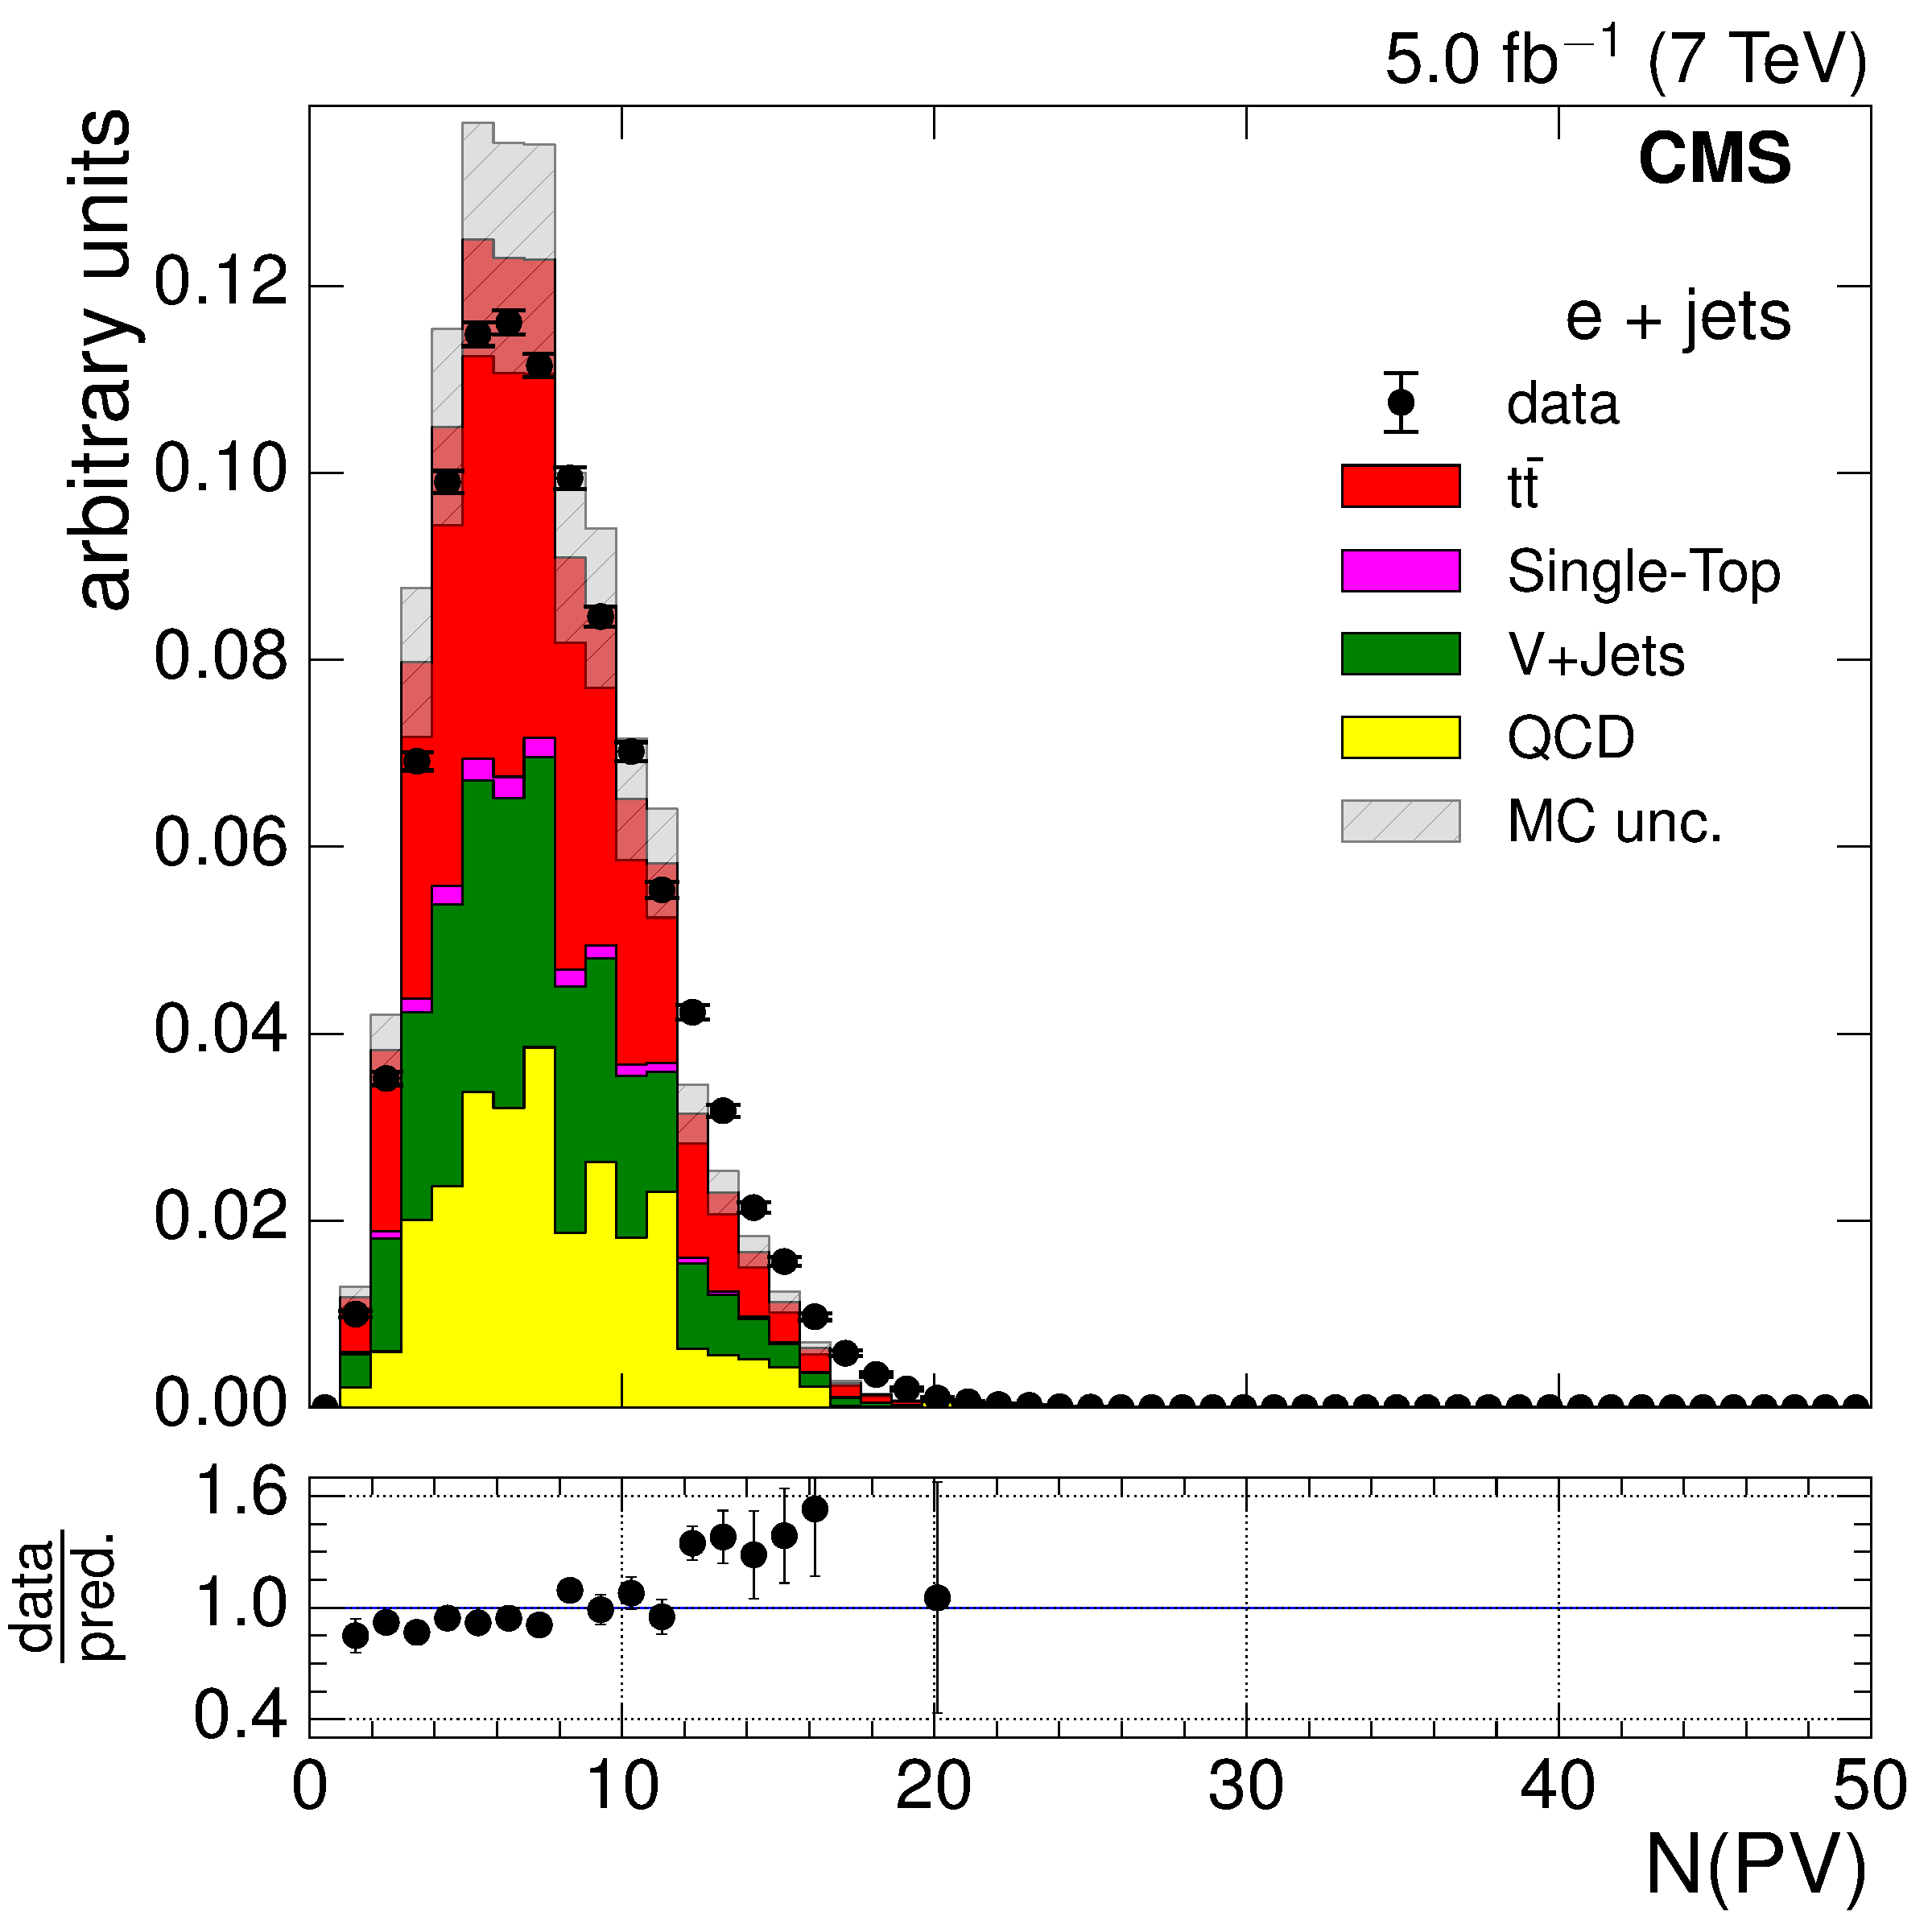
\includegraphics[width=0.48\textwidth]{Chapters/07_08_09_Analysis/Images/control_plots/before_fit/7TeV/EPlusJets_nVertex_with_ratio}\hfill
      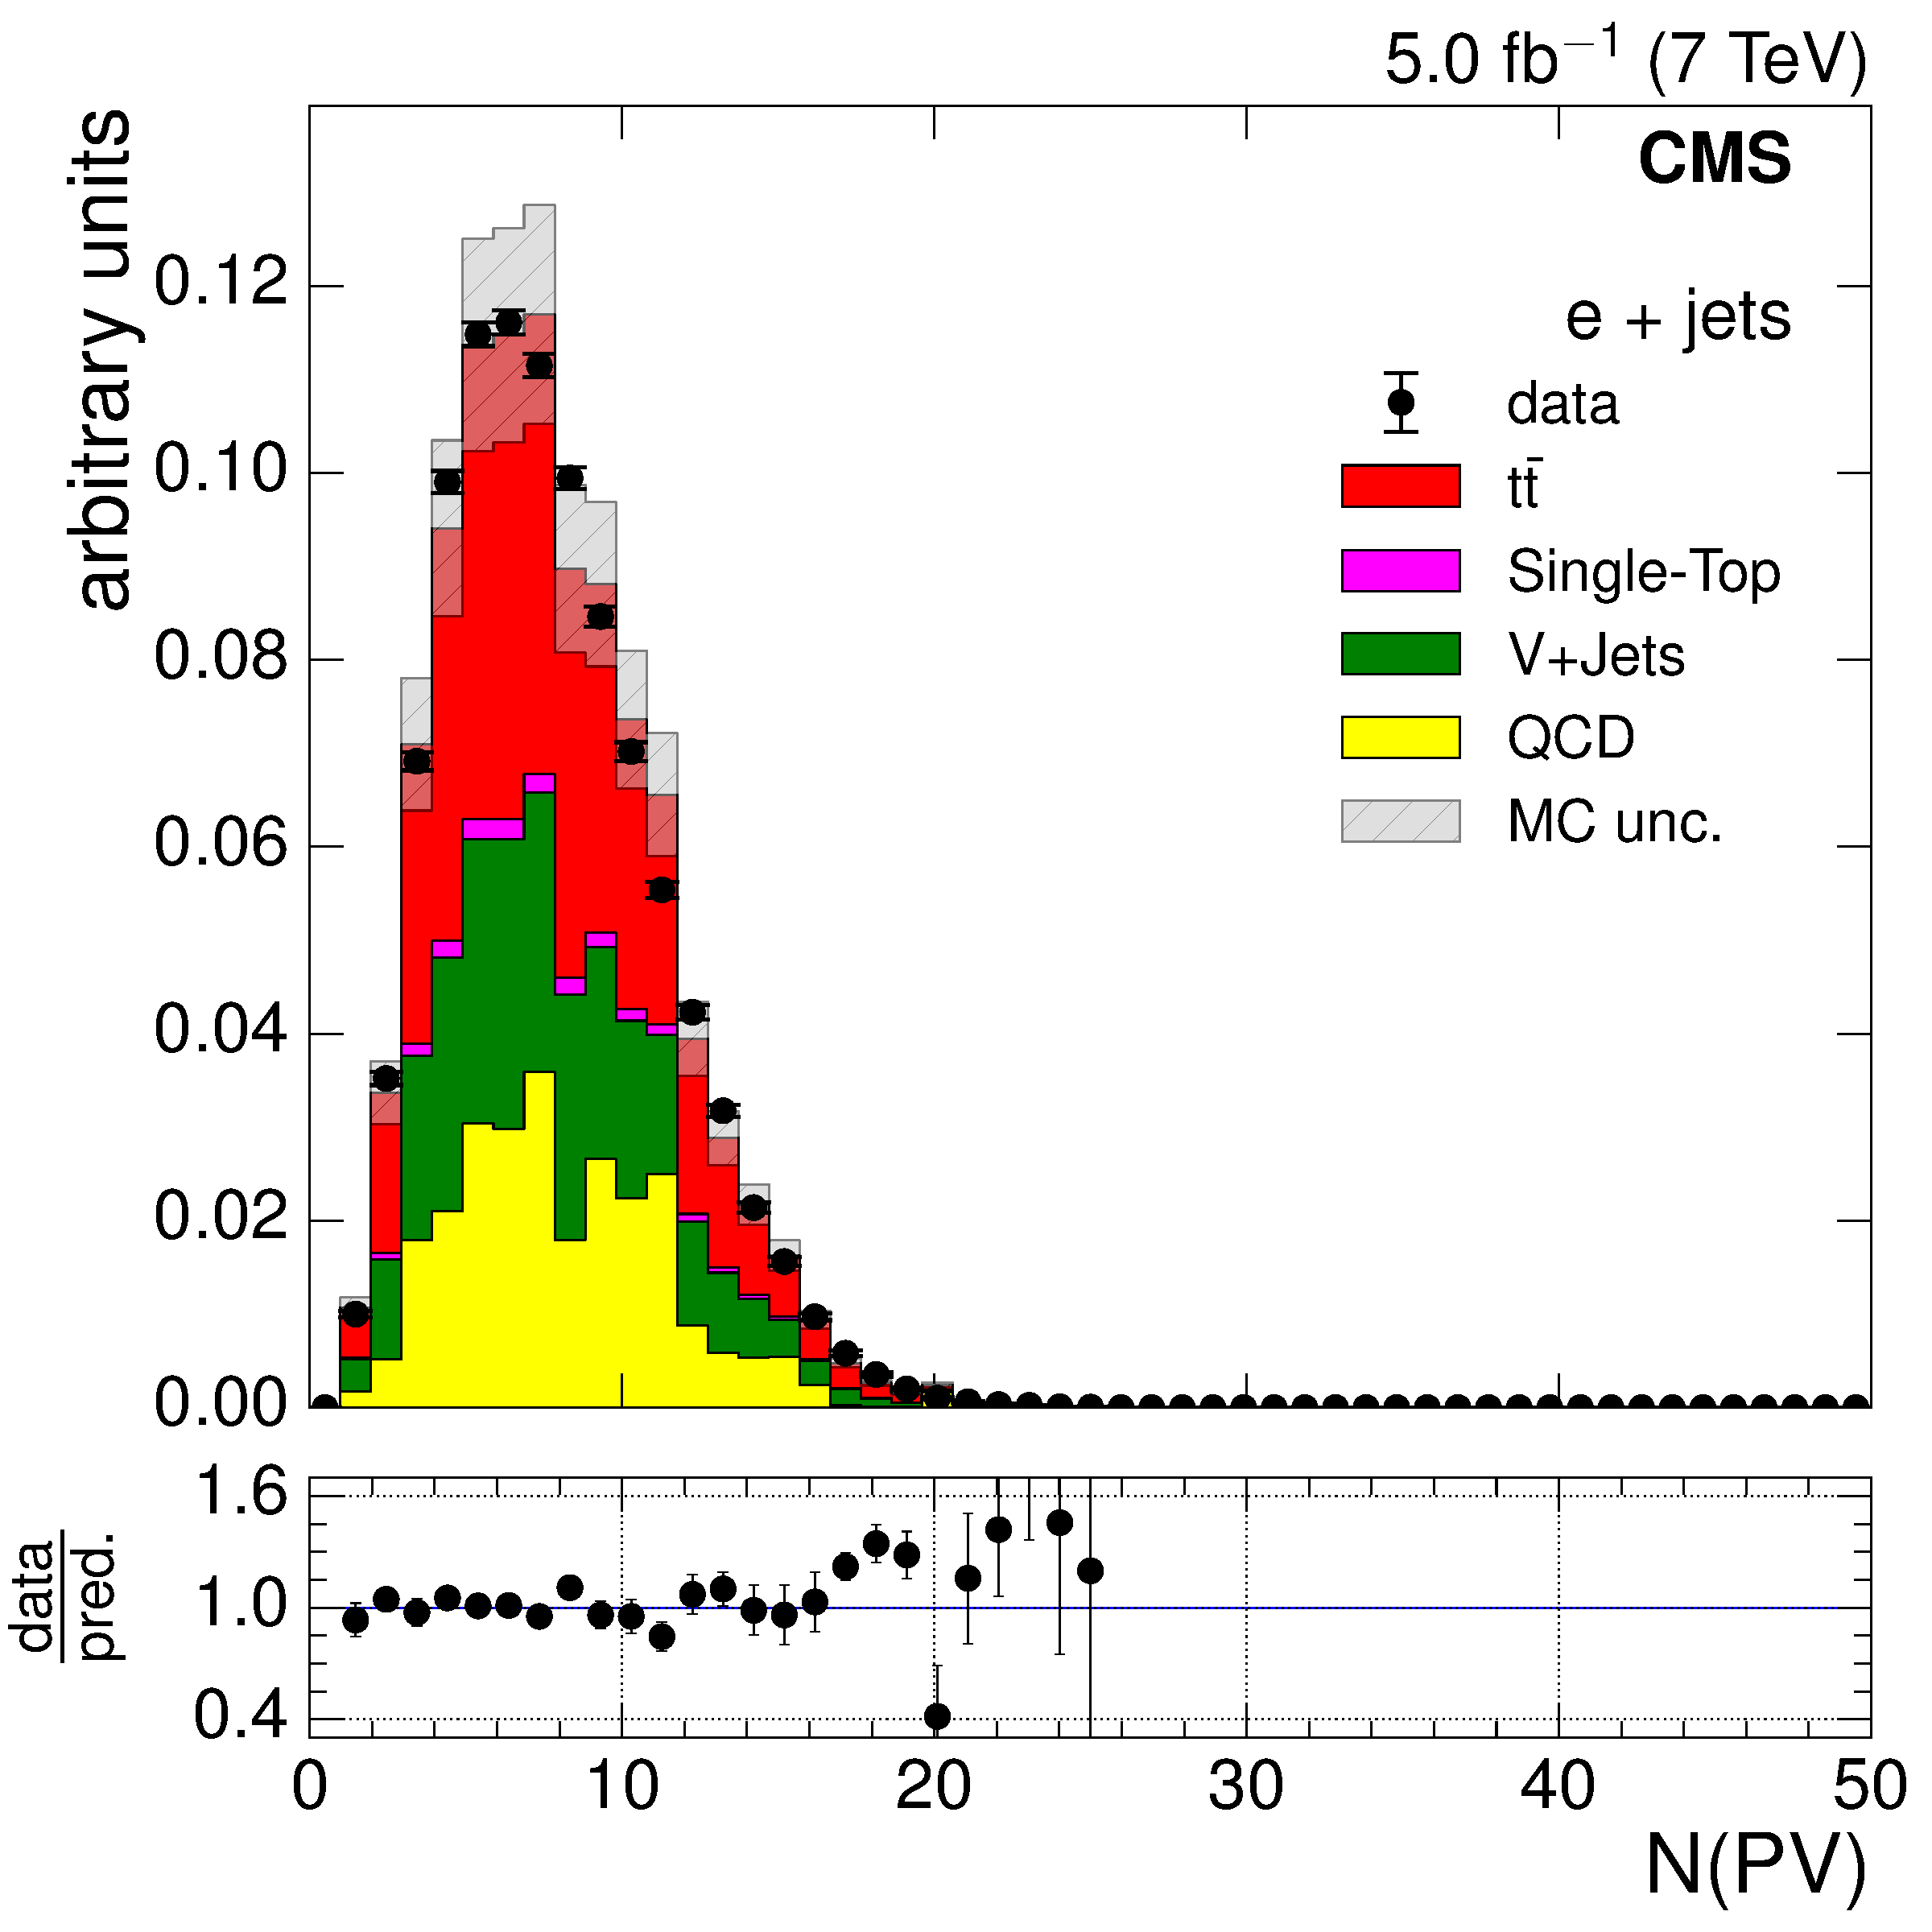
\includegraphics[width=0.48\textwidth]{Chapters/07_08_09_Analysis/Images/control_plots/before_fit/7TeV/EPlusJets_nVertex_reweighted_with_ratio}\\
      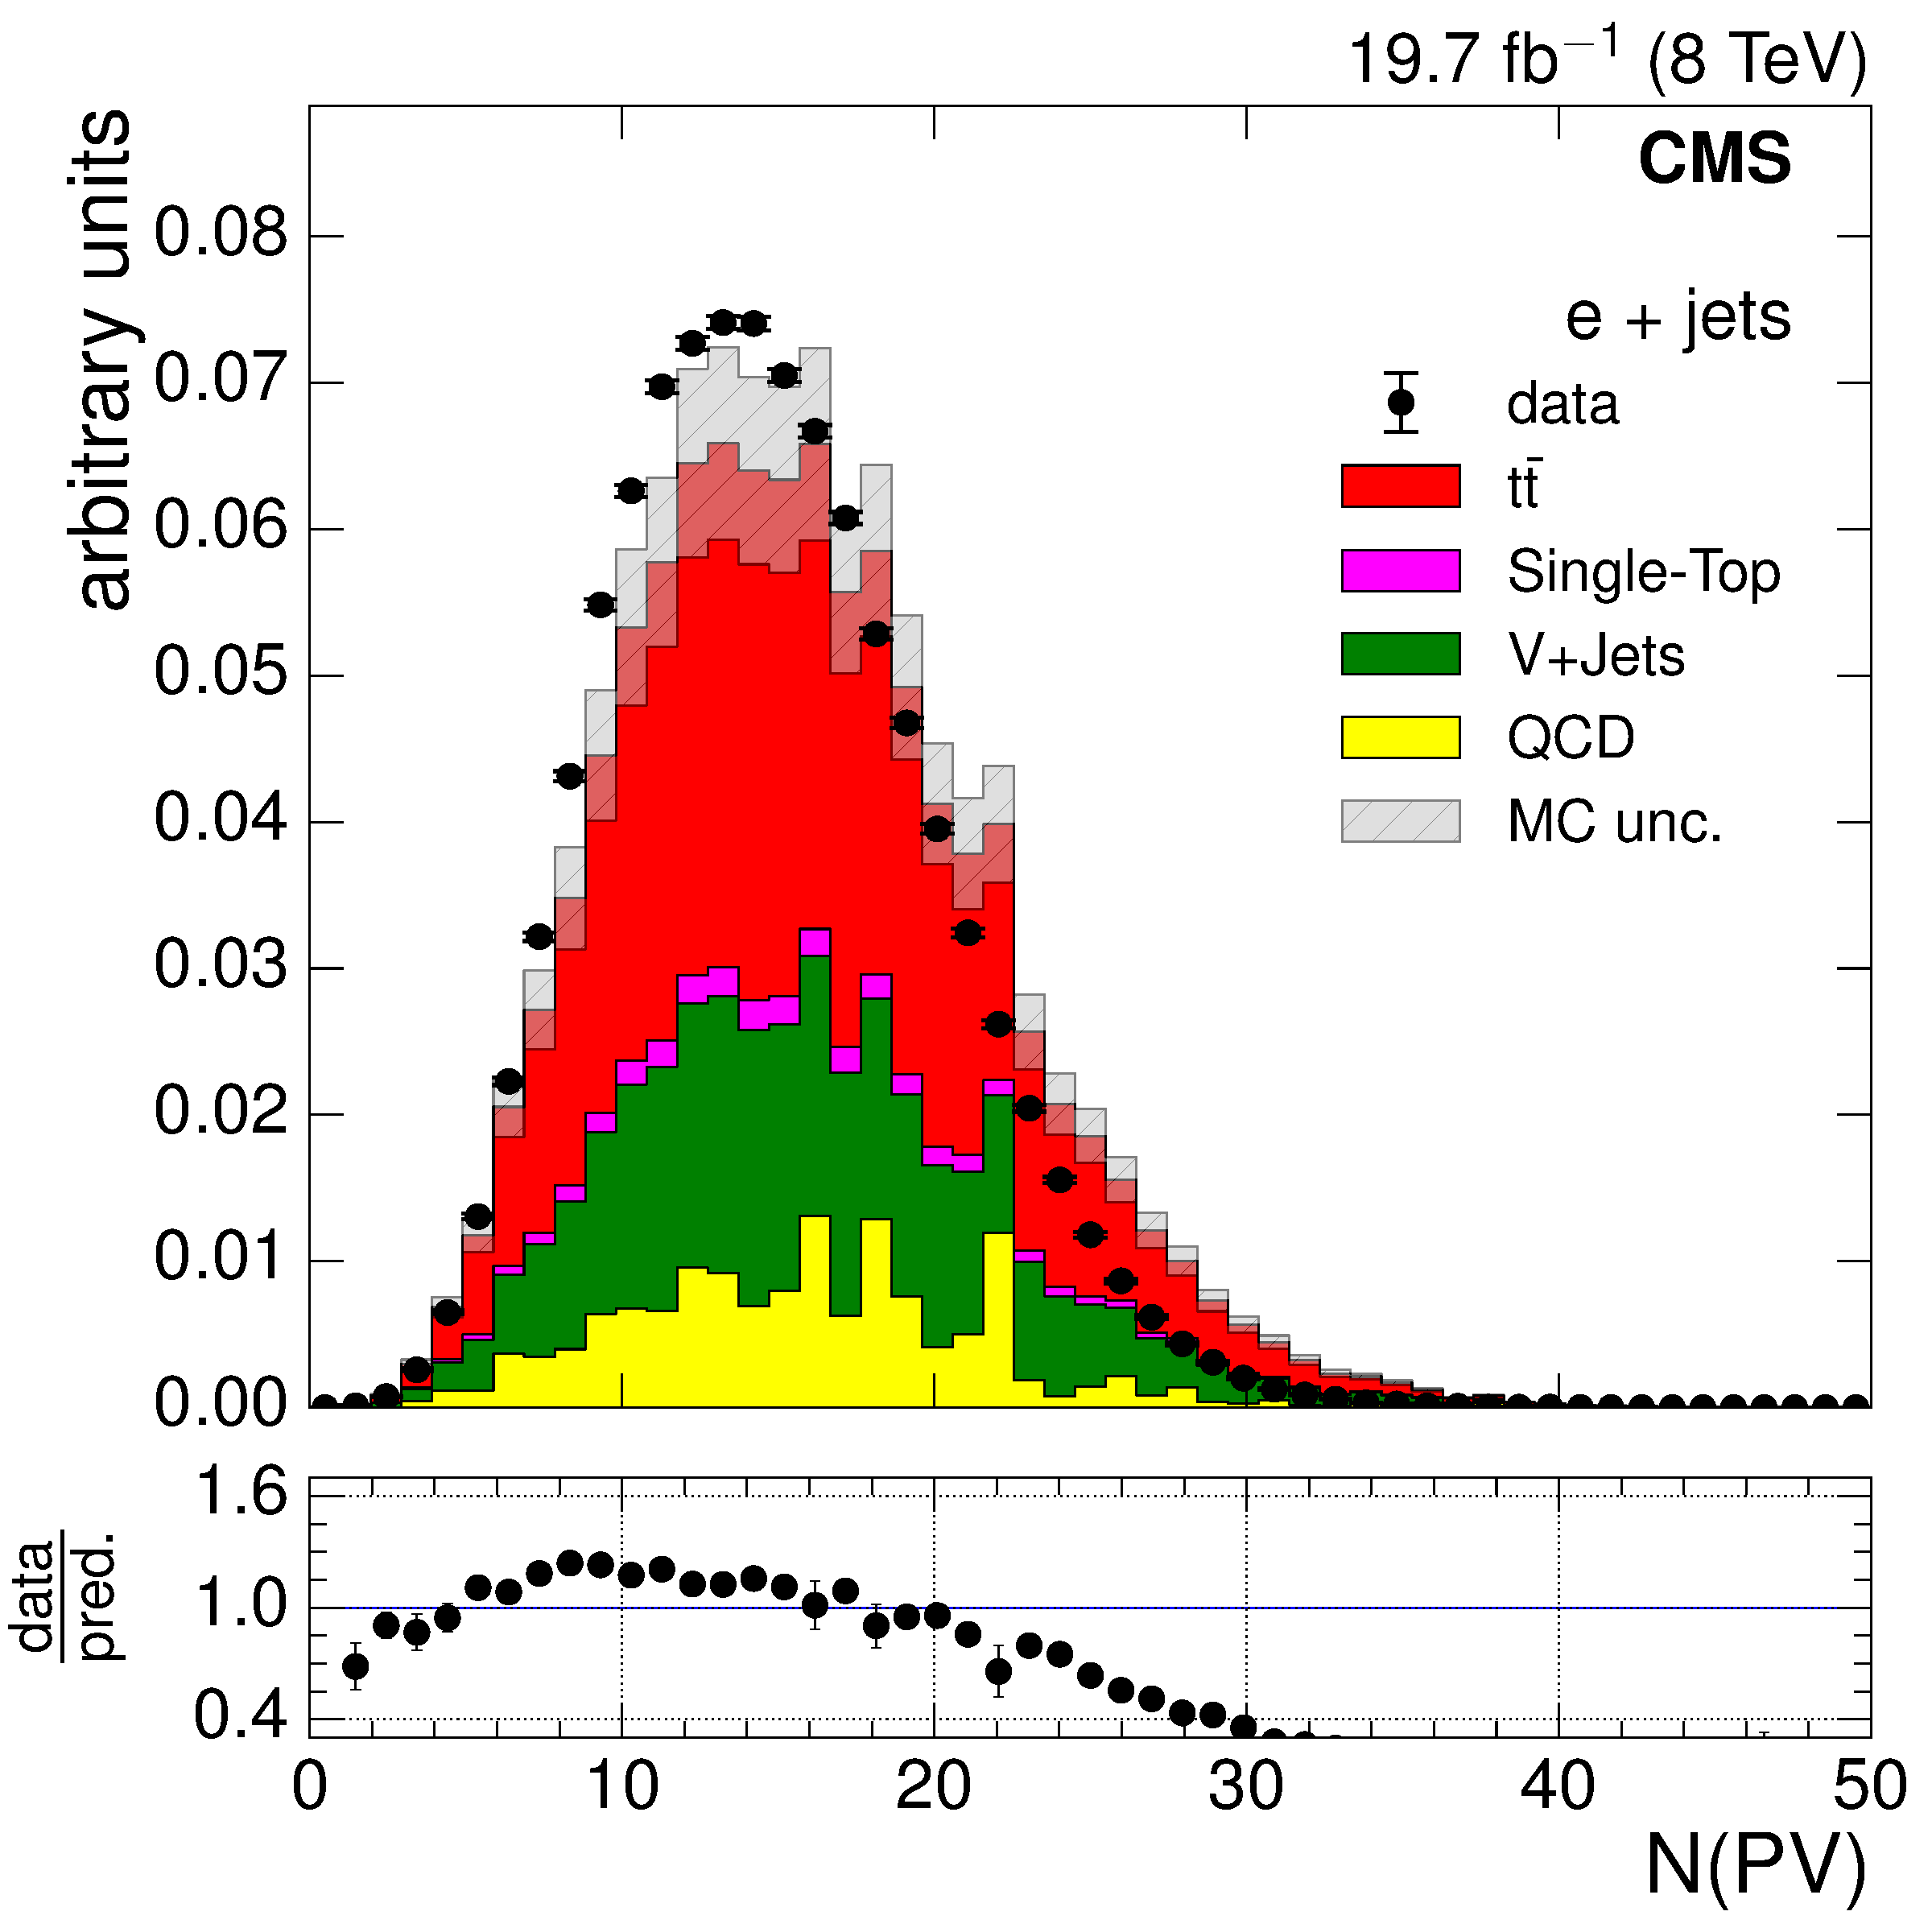
\includegraphics[width=0.48\textwidth]{Chapters/07_08_09_Analysis/Images/control_plots/before_fit/8TeV/EPlusJets_nVertex_with_ratio}\hfill
      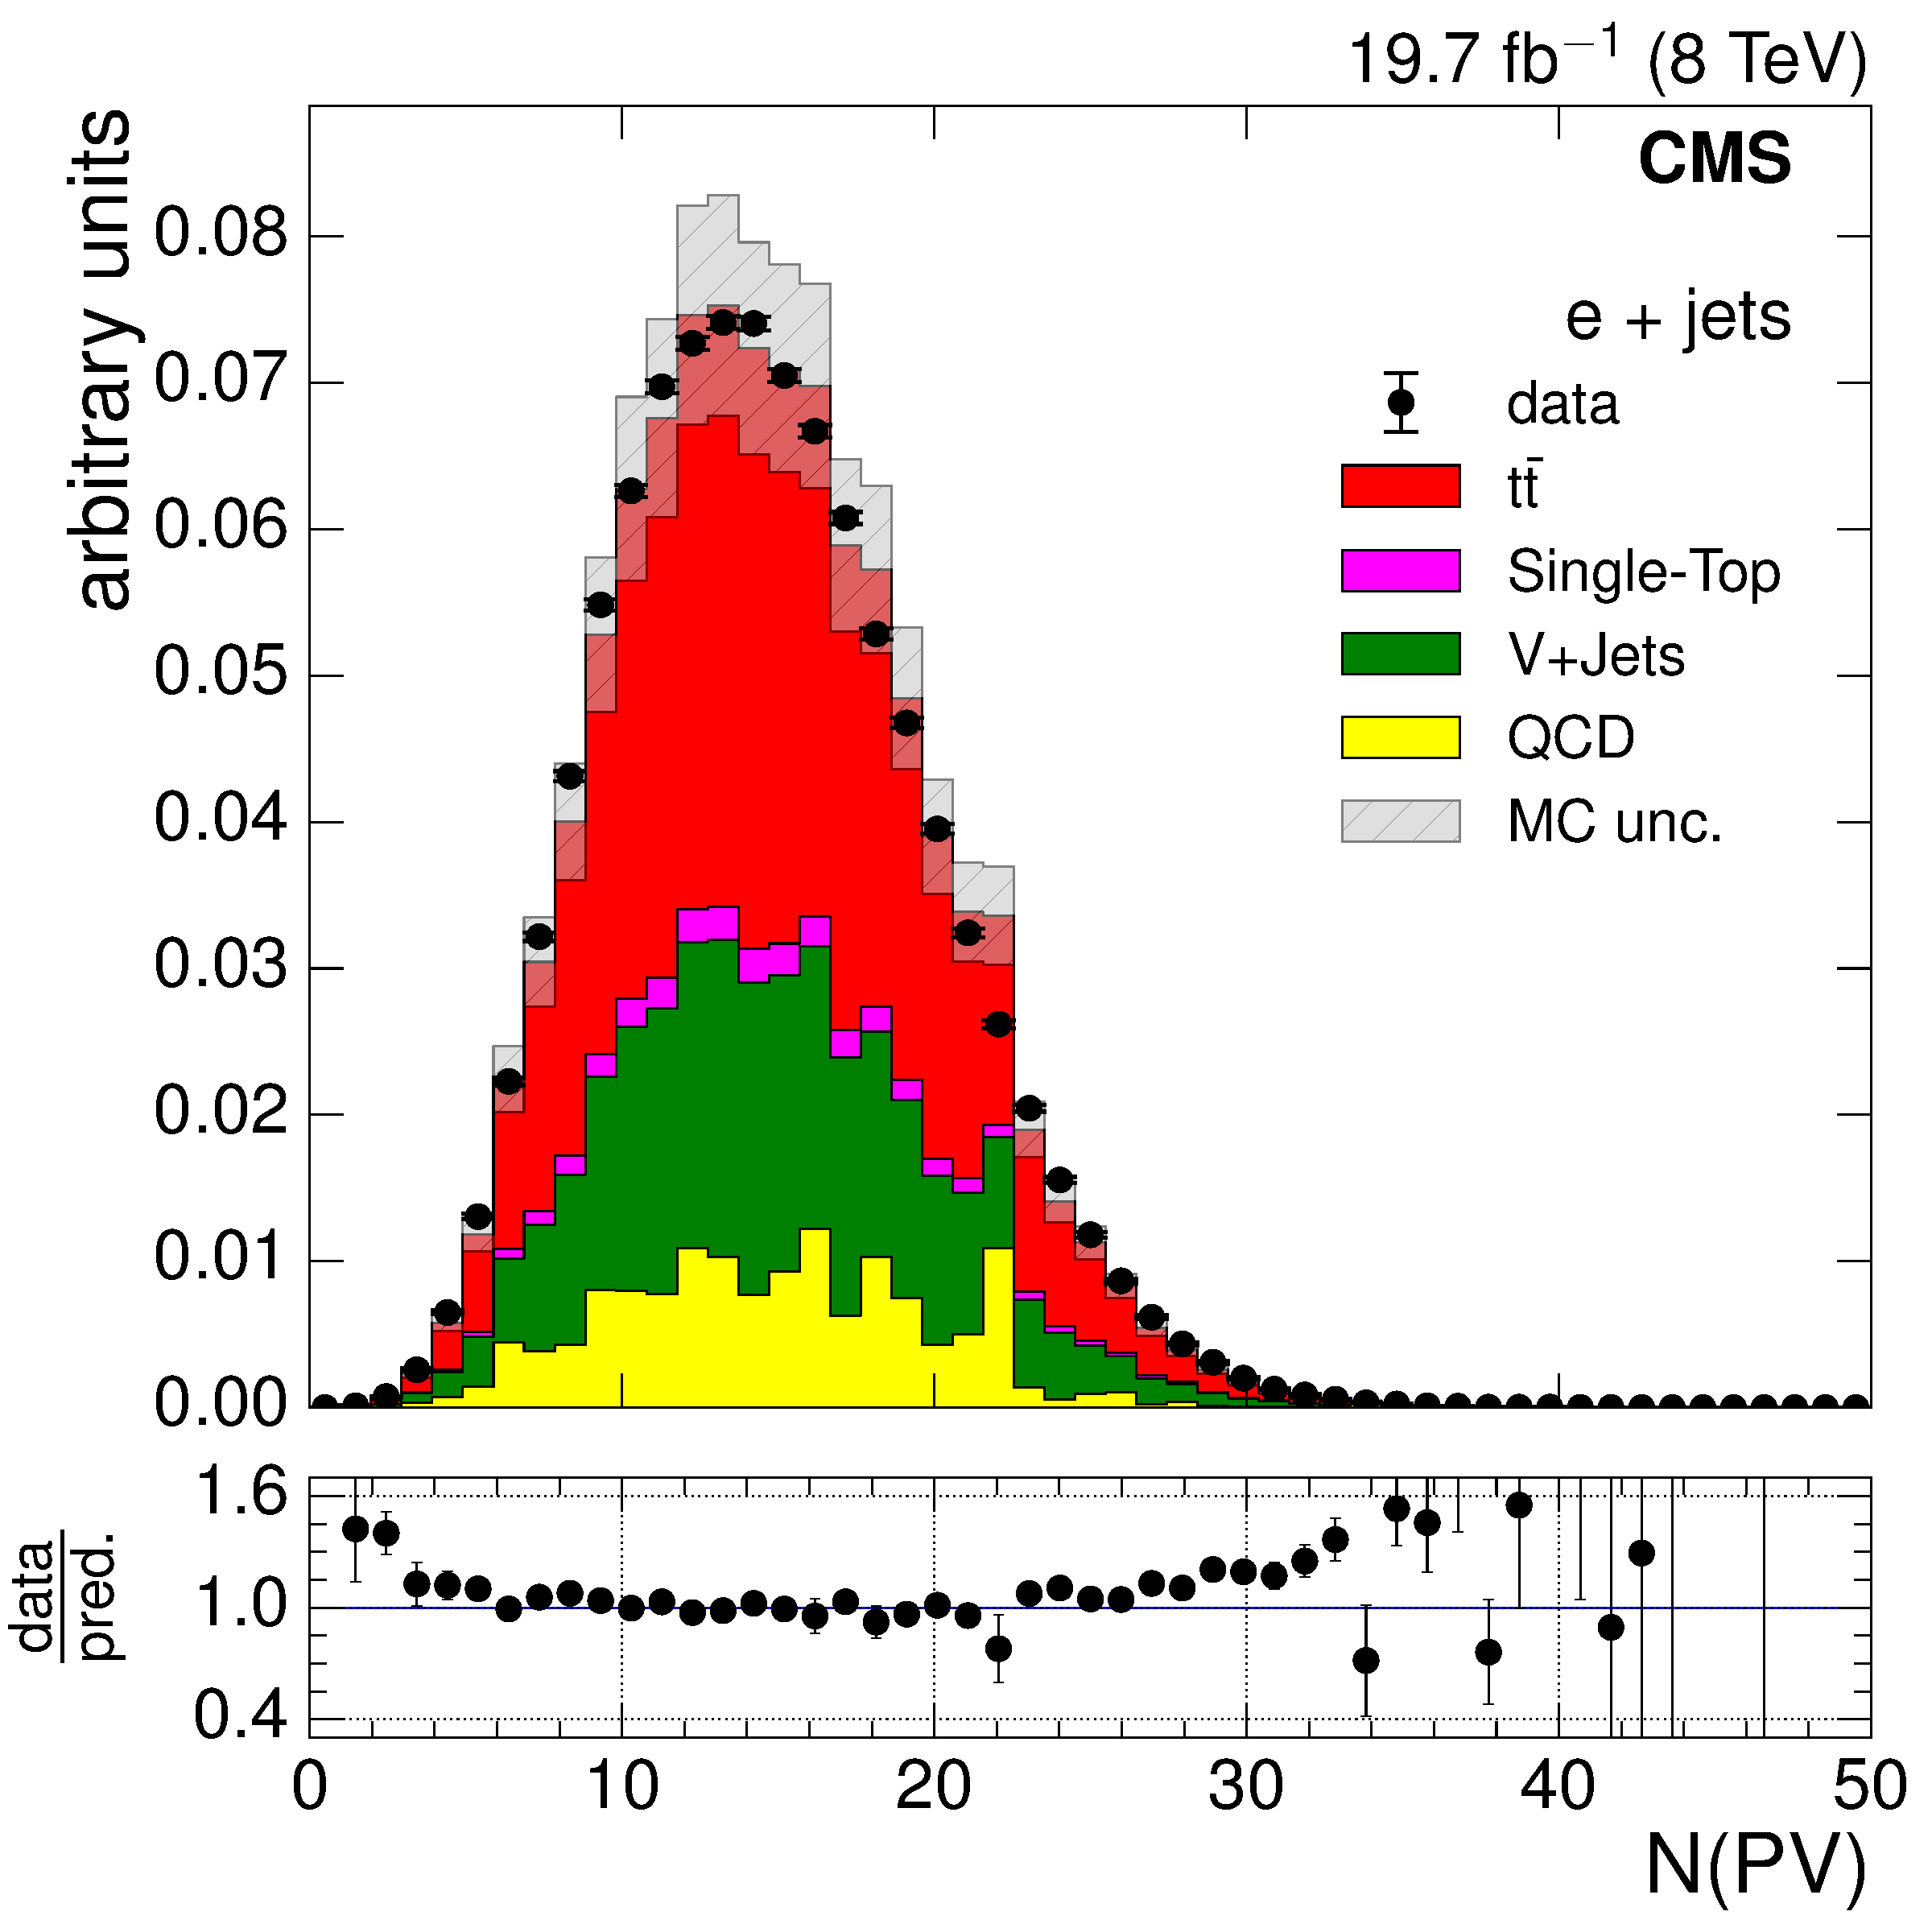
\includegraphics[width=0.48\textwidth]{Chapters/07_08_09_Analysis/Images/control_plots/before_fit/8TeV/EPlusJets_nVertex_reweighted_with_ratio}\\
     \caption[Distributions of the number of reconstructed vertices in an event in the electron+jets channel
     before and after implementing pileup reweighting at $\roots=7\TeV$ and $\roots=8\TeV$.]{Distributions of
     the number of reconstructed vertices in an event in the electron+jets channel before implementing pileup
     reweighting (left) and after implementation (right) at $\roots=7\TeV$ (upper) and $\roots=8\TeV$ (lower).
     Both data and sum of MC simulations are normalised to one.}
     \label{fig:nvertices_before_and_after_pileup_reweighting_electrons}
\end{figure}

\subsection{\btagging}
\label{ss:b_tagging}
The combined secondary vertex \btagging algorithm (CSV) described in
Section~\ref{ss:combined_secondary_vertex} is used in this analysis to identify jets originating from \bquarks
in \ttbar events. The medium working point, CSVM, which corresponds to a cut on the discriminator output by
the algorithm of 0.679, is used in this analysis. This corresponds to a \btagging efficiency of $\approx$70~\%
and a mis-tag efficiency of 1~\% for jets from light quarks ($\cPqu$, $\cPqd$, $\cPqs$) and gluons.
Discrepancies between the \btagging and mis-tagging efficiencies in data and Monte Carlo simulation have been
noted in $\roots=7\TeV$~\cite{Chatrchyan:2012jua} and $\roots=8\TeV$~\cite{CMS-PAS-BTV-13-001}. To account for
these differences, events are reweighted as a function of \pt and $\eta$, based on the recommendation of the
CMS \btagging POG, with the aim of ensuring that the probability of an event passing selection criteria in
simulation matches the probability of an event in data with the same jet(s) passing the same selection. Monte
Carlo simulation events are reweighted by a combination of an efficiency, which accounts for tagging
efficiencies of \bjets, \cjets and light jets in simulation, and a scale factor, which takes into account the
difference in the aforementioned efficiencies in simulation and data. The result of this reweighting in the
electron+jets channel is shown in Figure~\ref{fig:nbjets_before_and_after_btag_scale_factors_electrons}, and
in the muon+jets channel in Figure~\ref{fig:nbjets_before_and_after_btag_scale_factors_muons} in
Appendix~\ref{as:data_monte_carlo_corrections}. The \btagging efficiency uncertainty is evaluated by varying
the scale factors by $\pm1\sigma$.

\begin{figure}[hbtp]
    \centering
      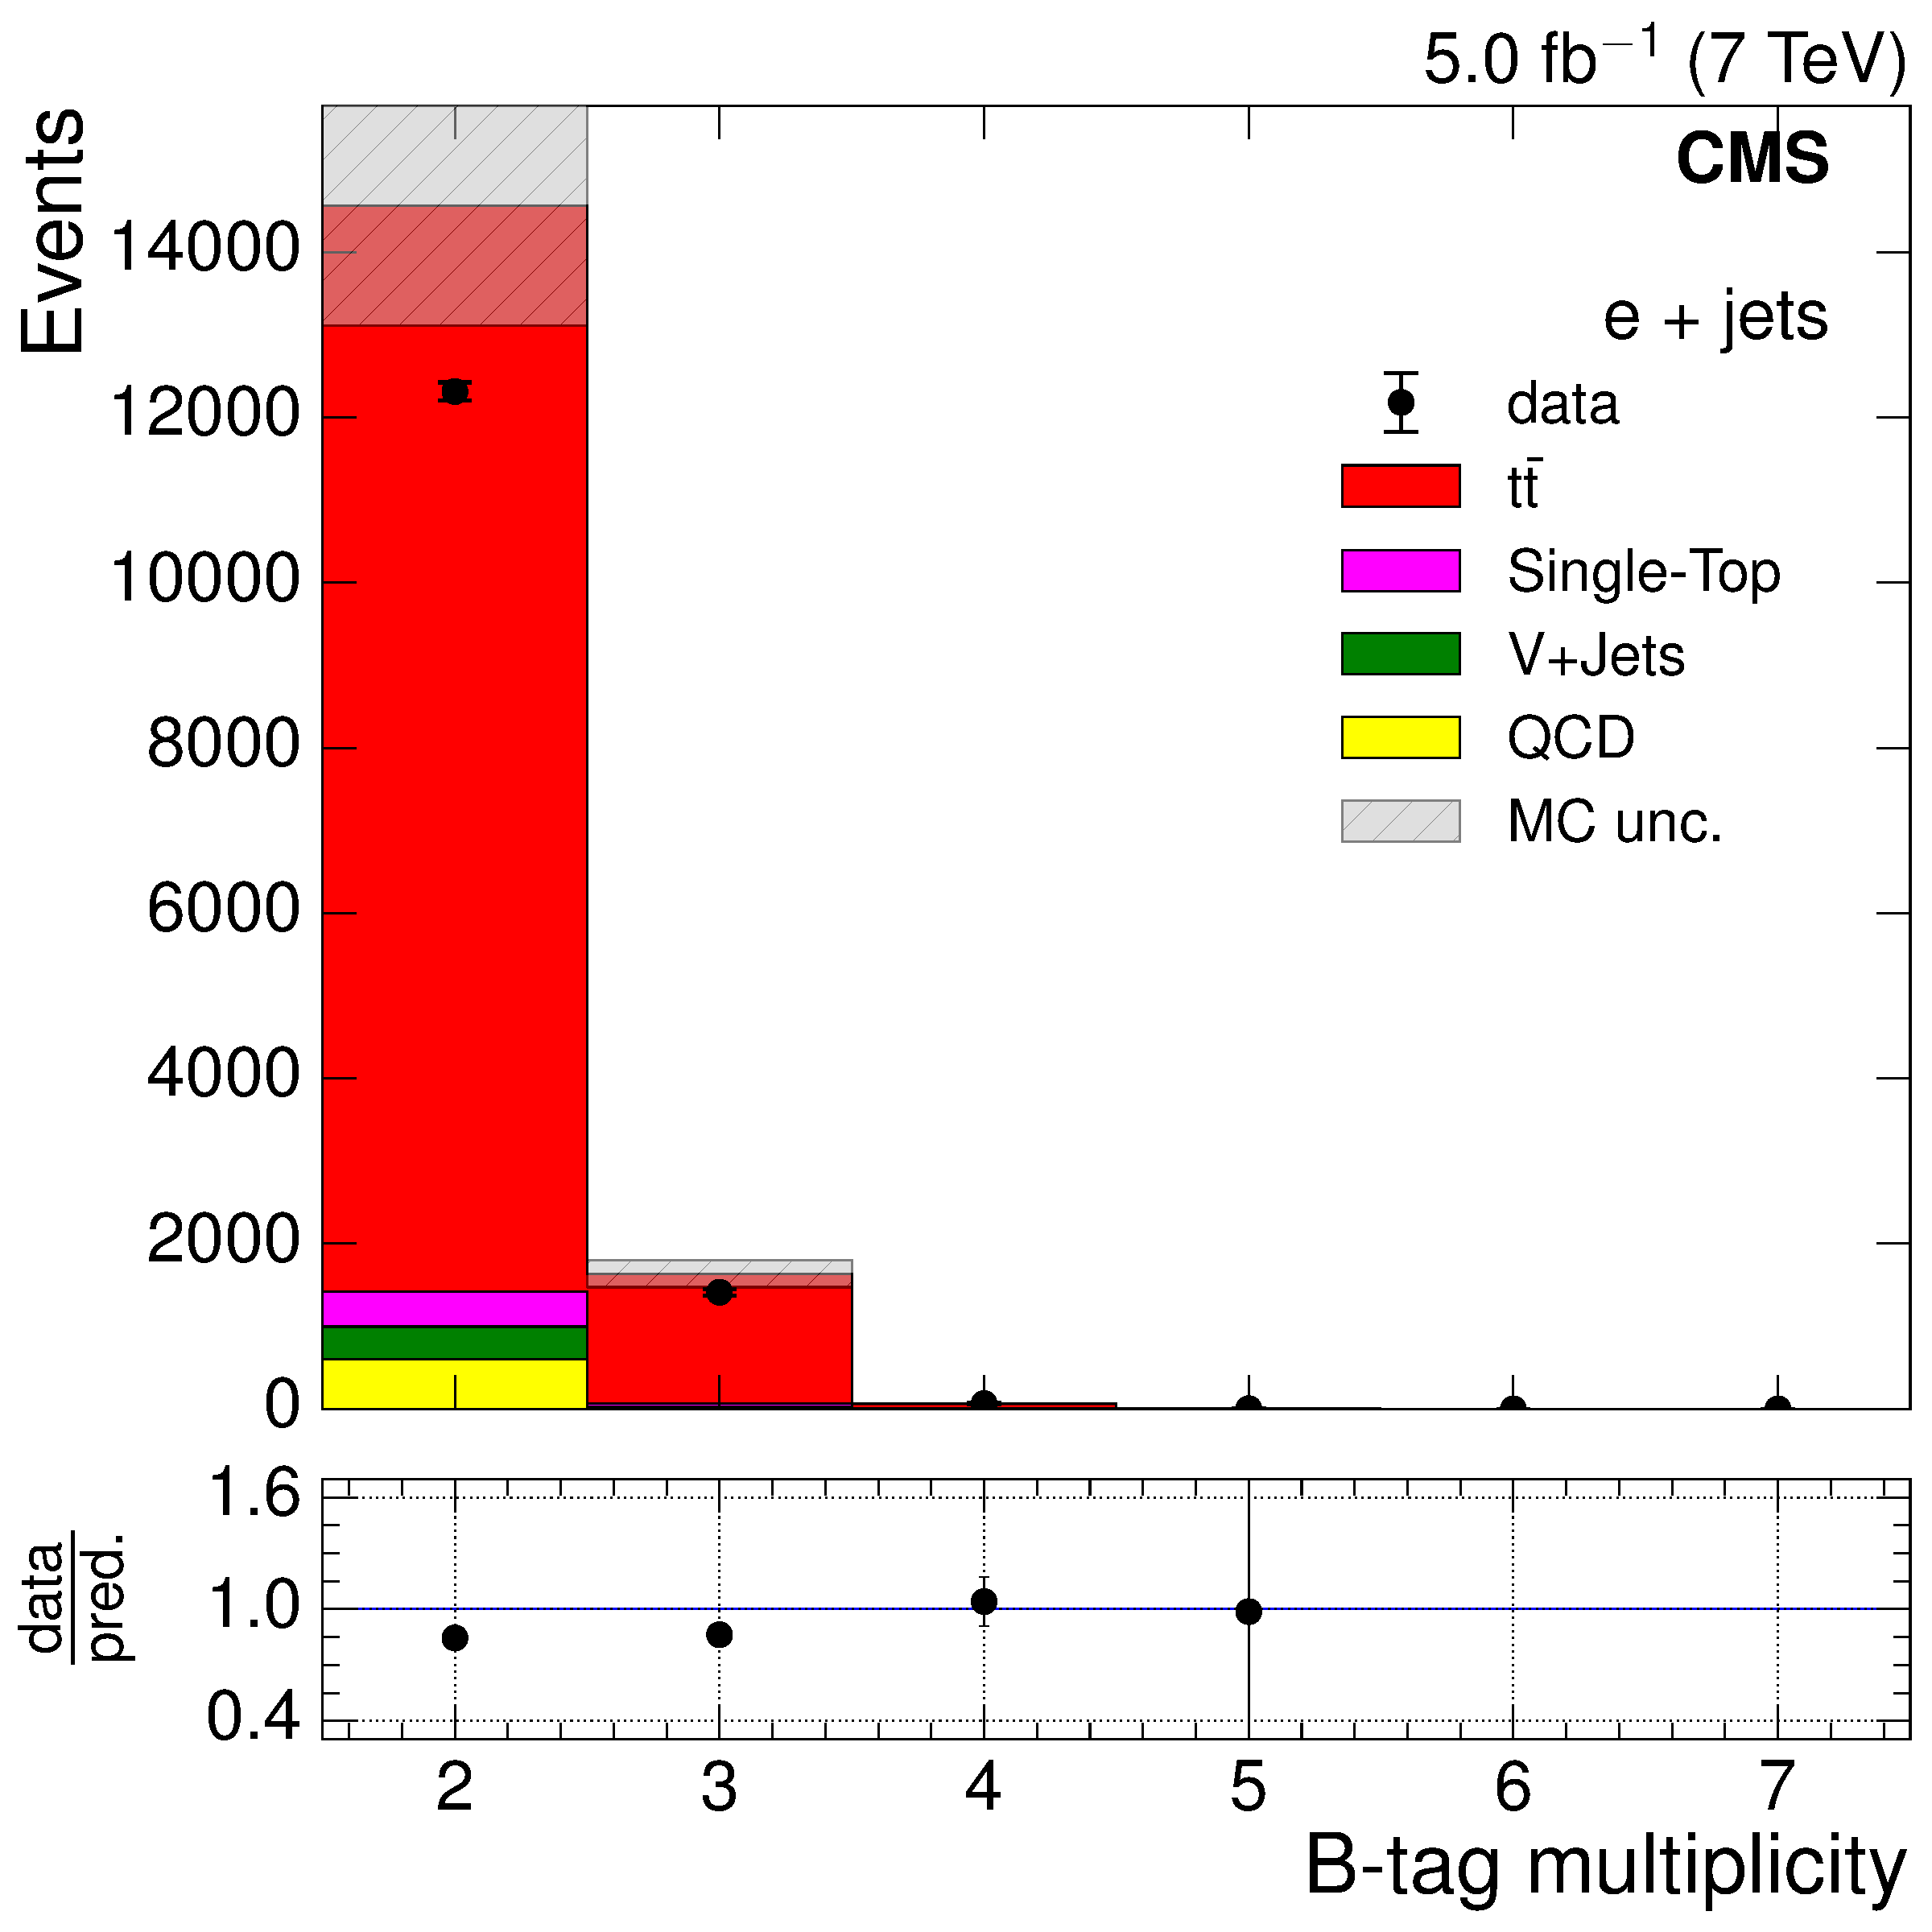
\includegraphics[width=0.48\textwidth]{Chapters/07_08_09_Analysis/Images/control_plots/before_fit/7TeV/EPlusJets_N_BJets_with_ratio}\hfill
      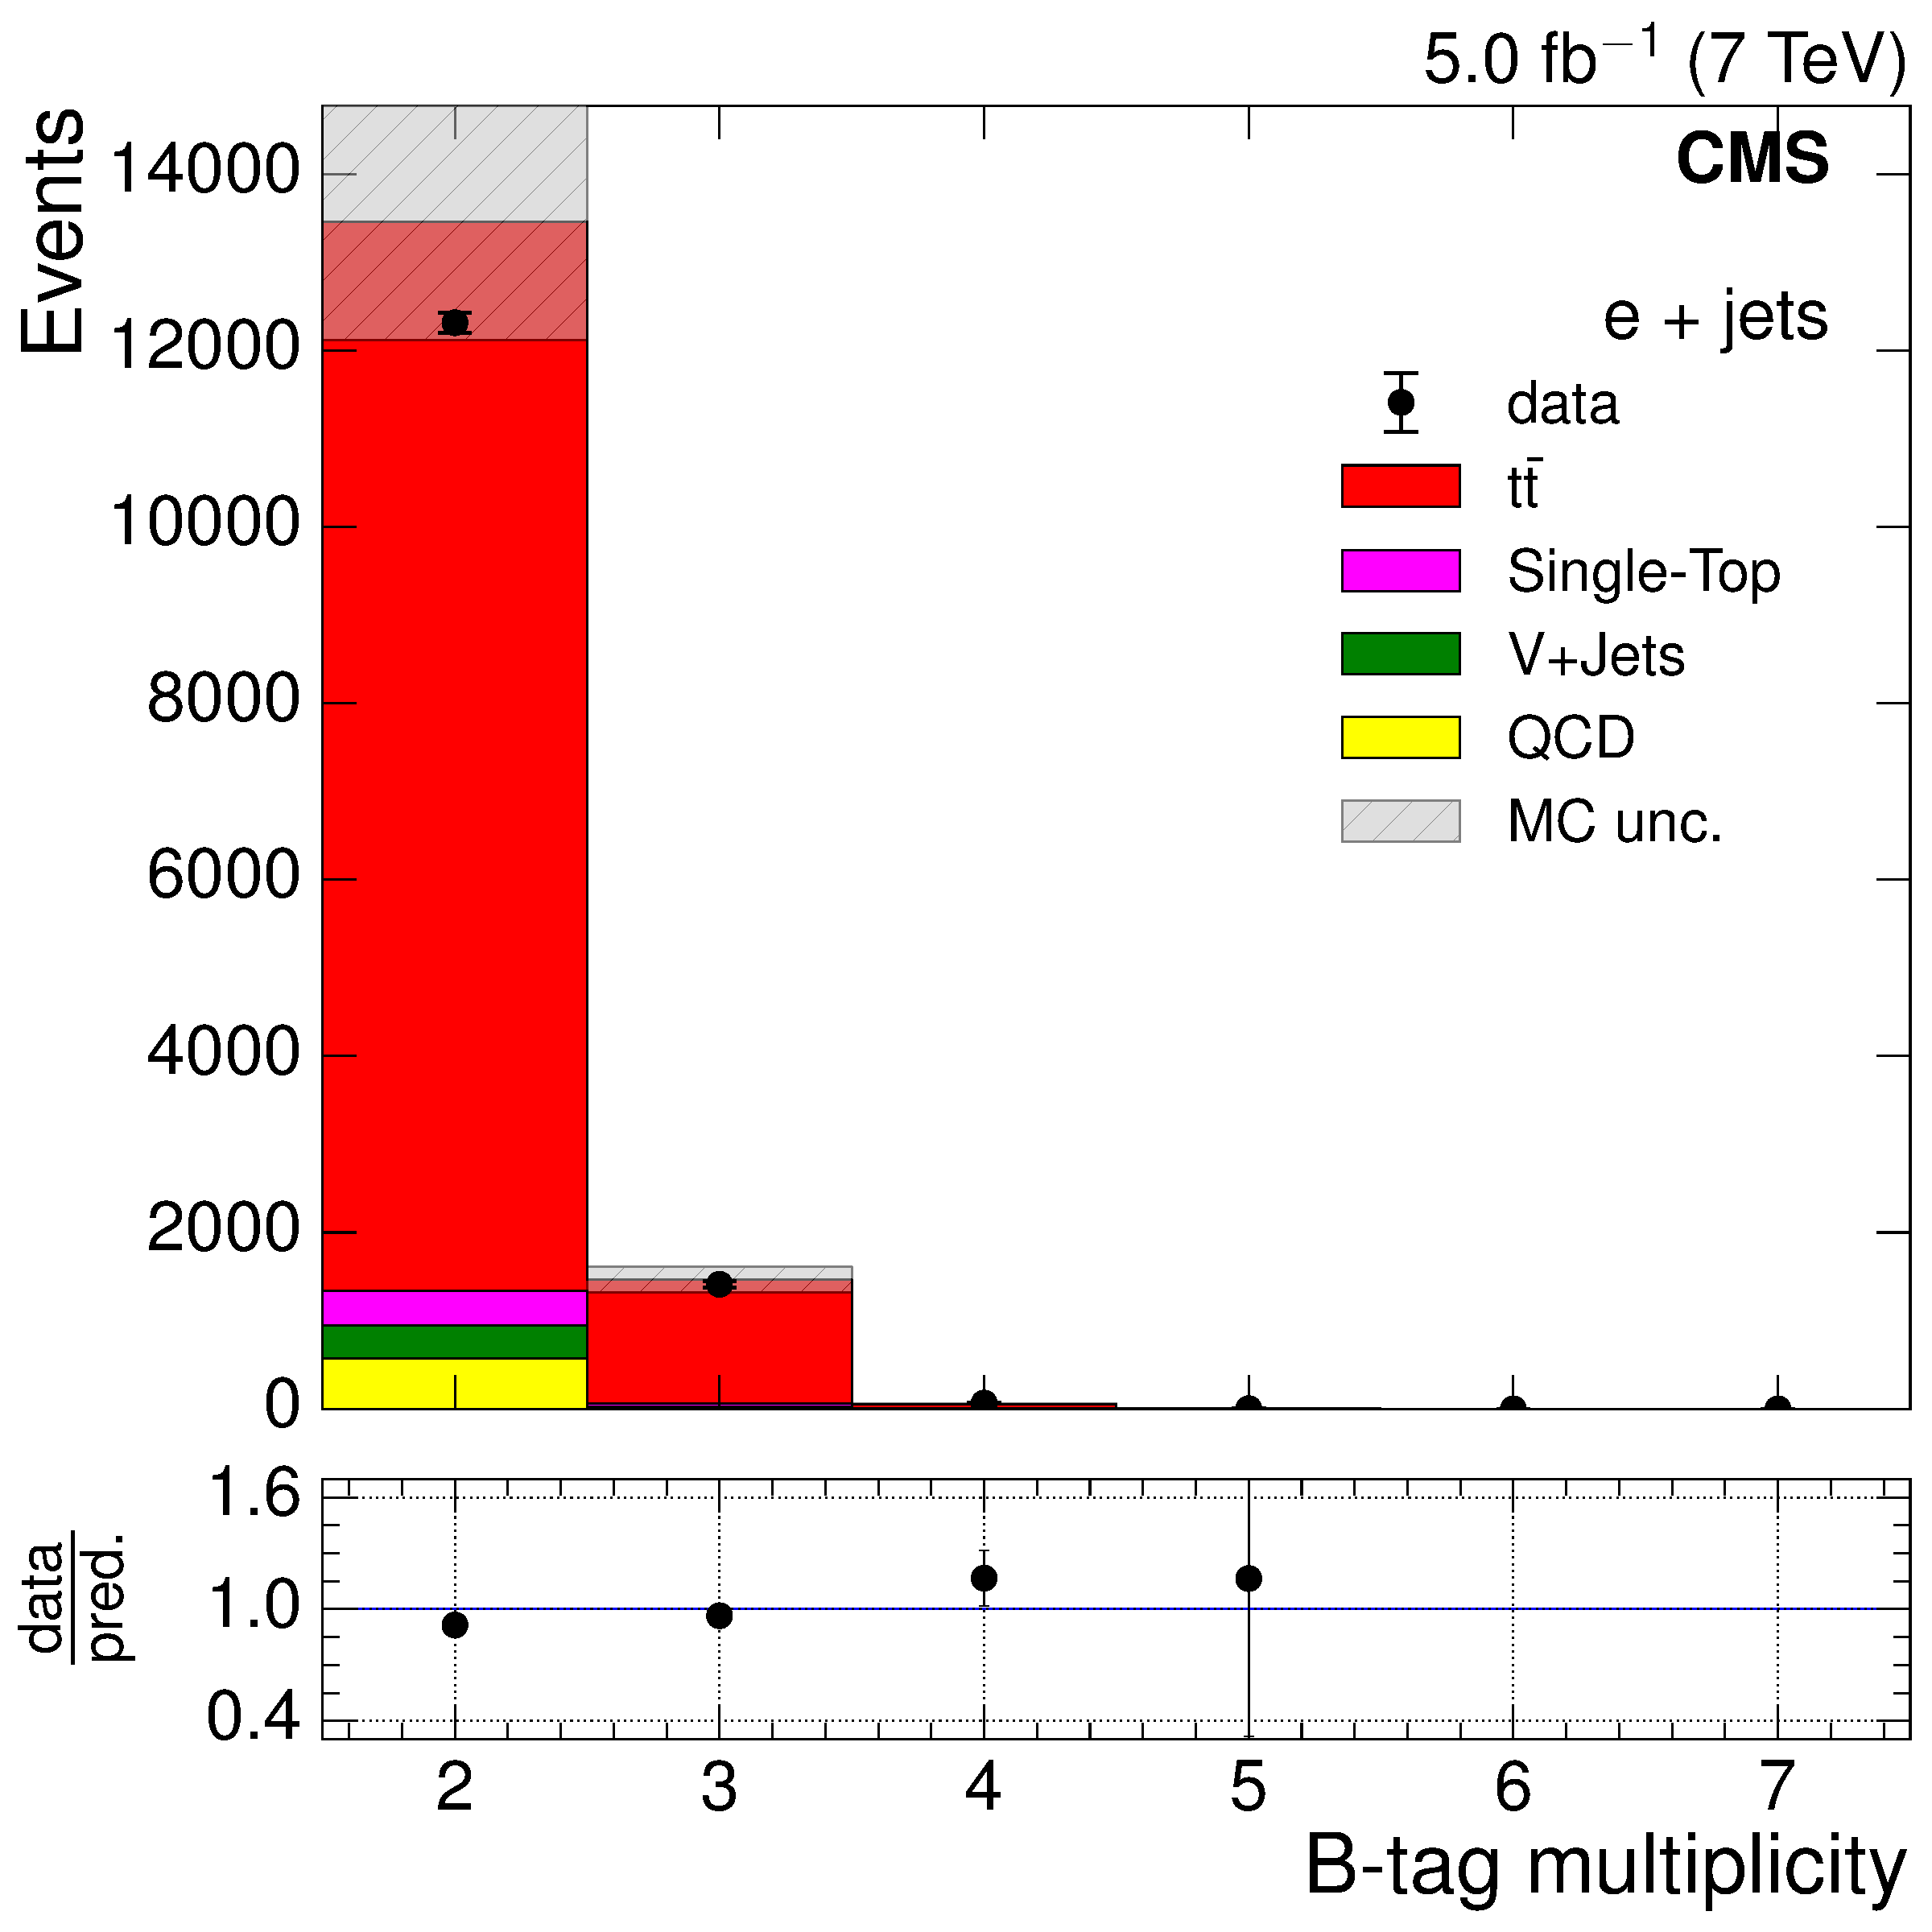
\includegraphics[width=0.48\textwidth]{Chapters/07_08_09_Analysis/Images/control_plots/before_fit/7TeV/EPlusJets_N_BJets_reweighted_with_ratio}\\
      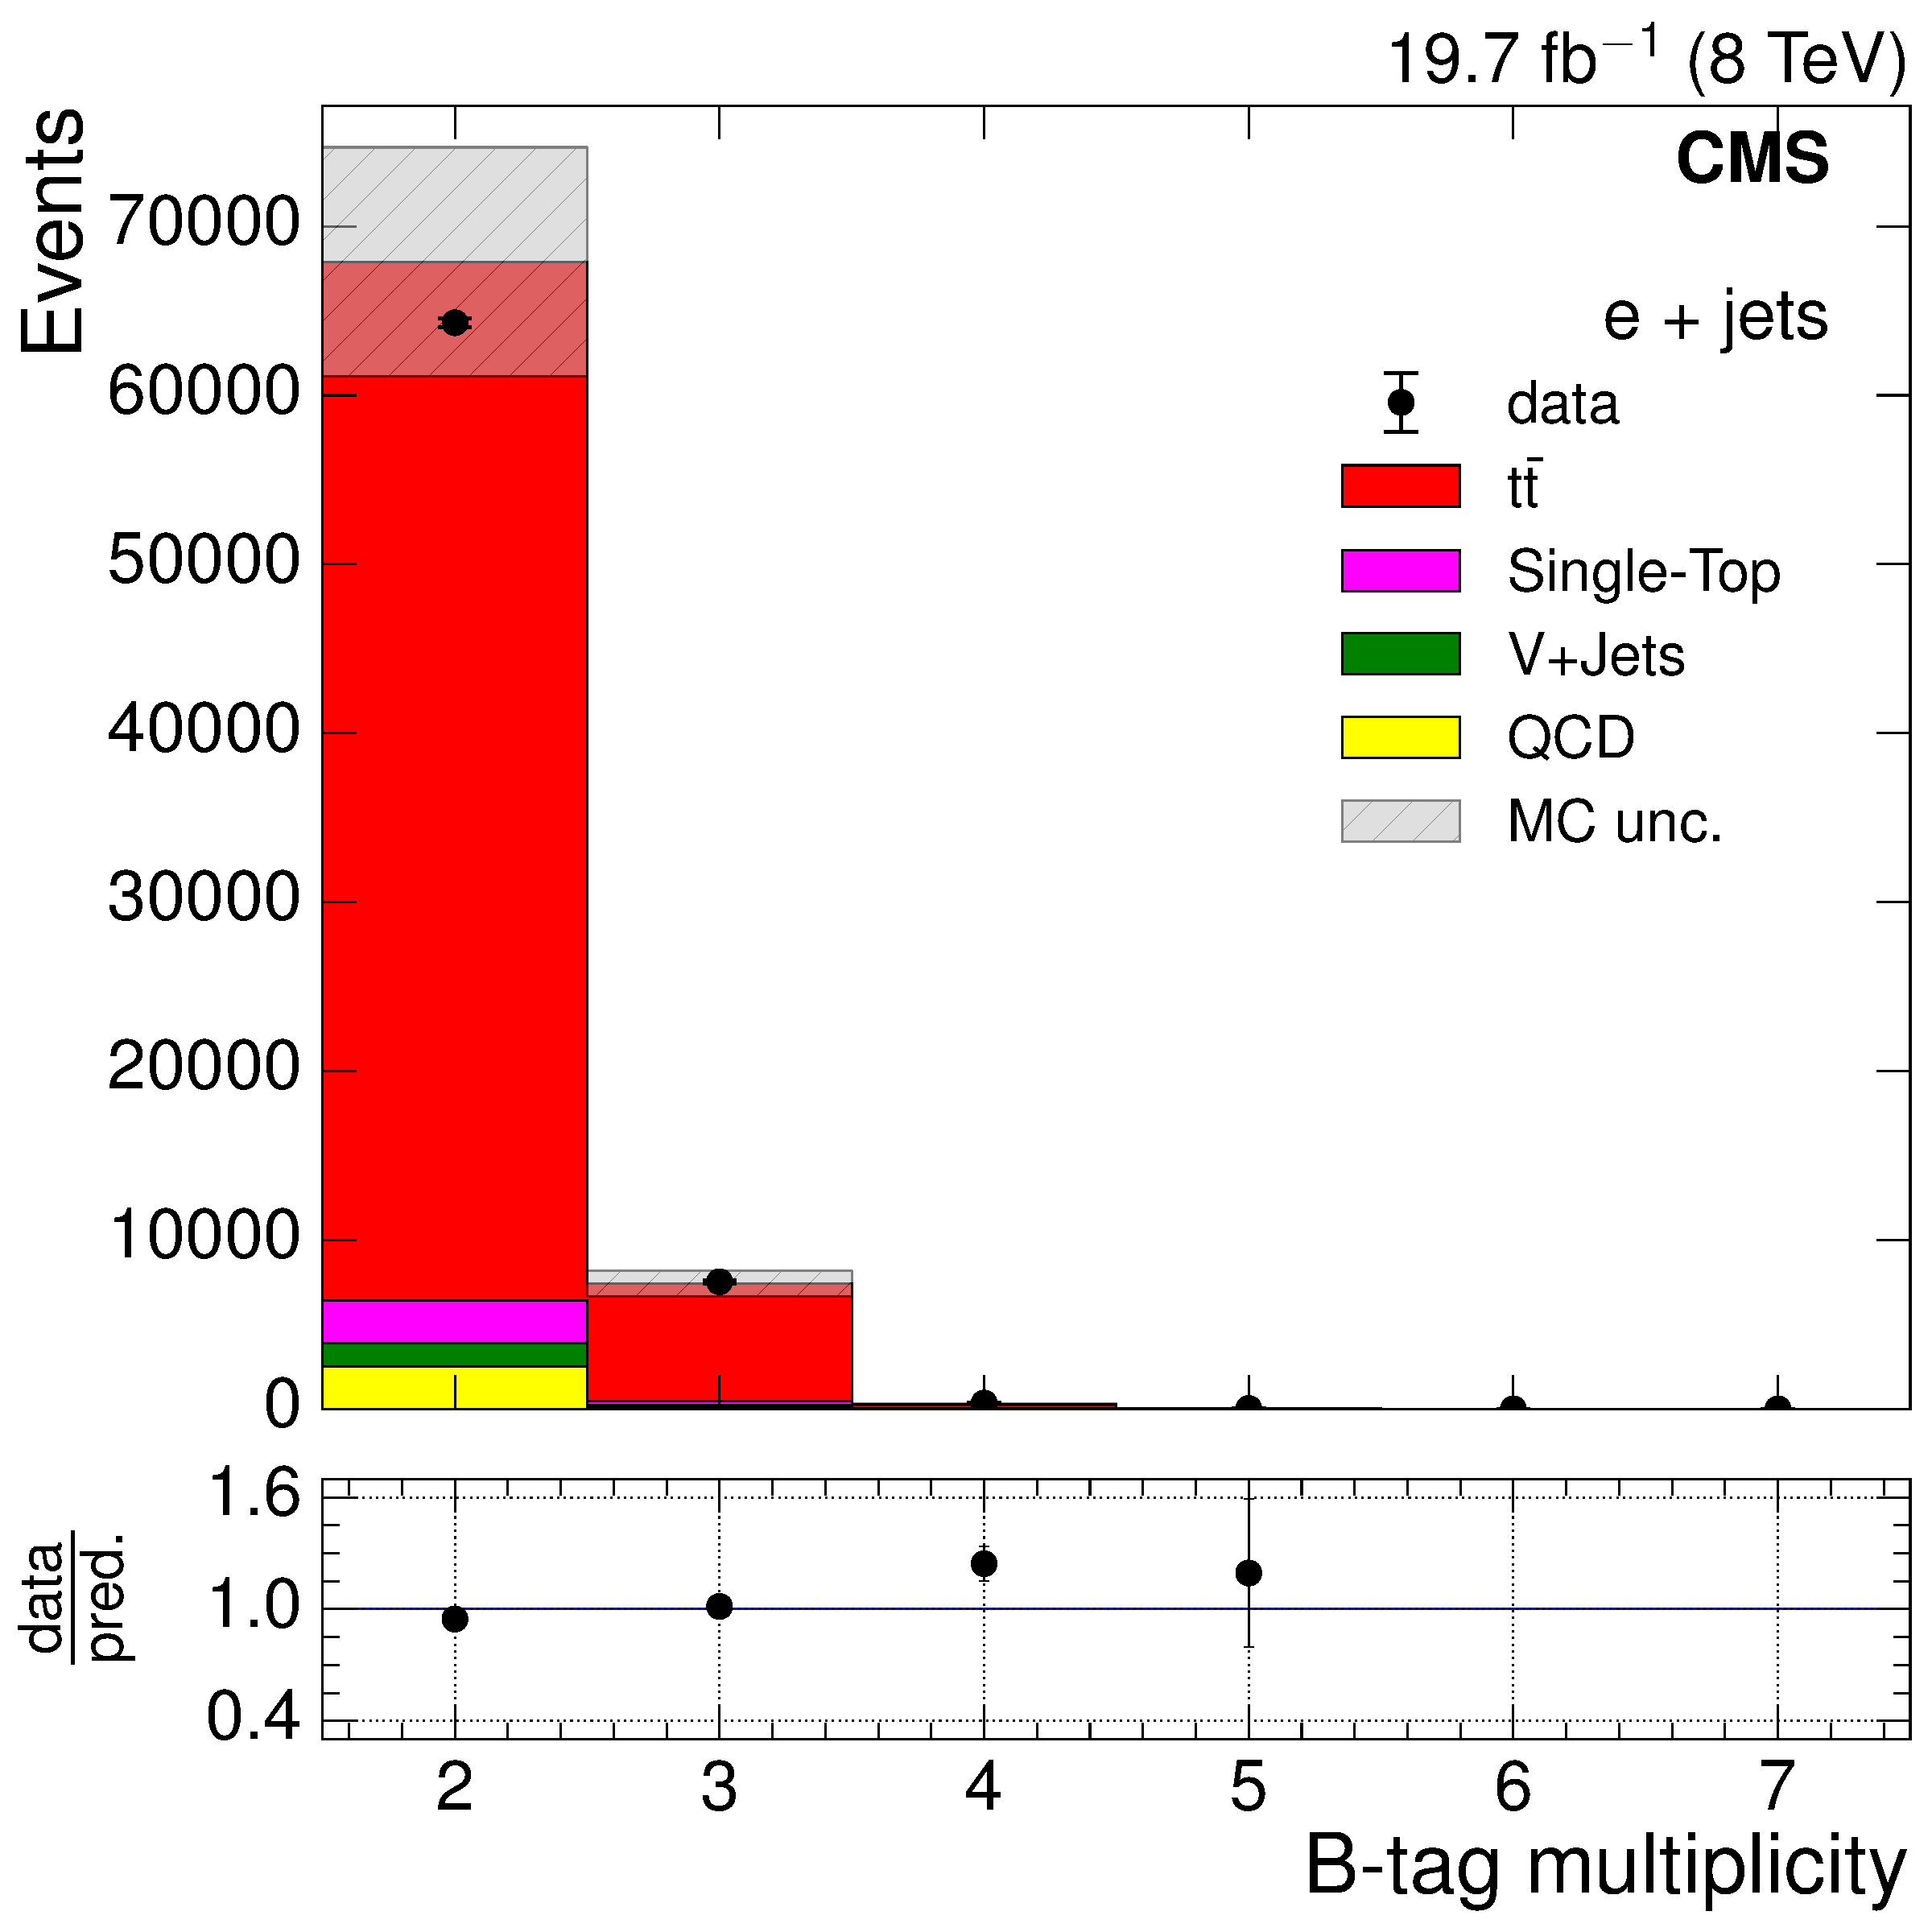
\includegraphics[width=0.48\textwidth]{Chapters/07_08_09_Analysis/Images/control_plots/before_fit/8TeV/EPlusJets_N_BJets_with_ratio}\hfill
      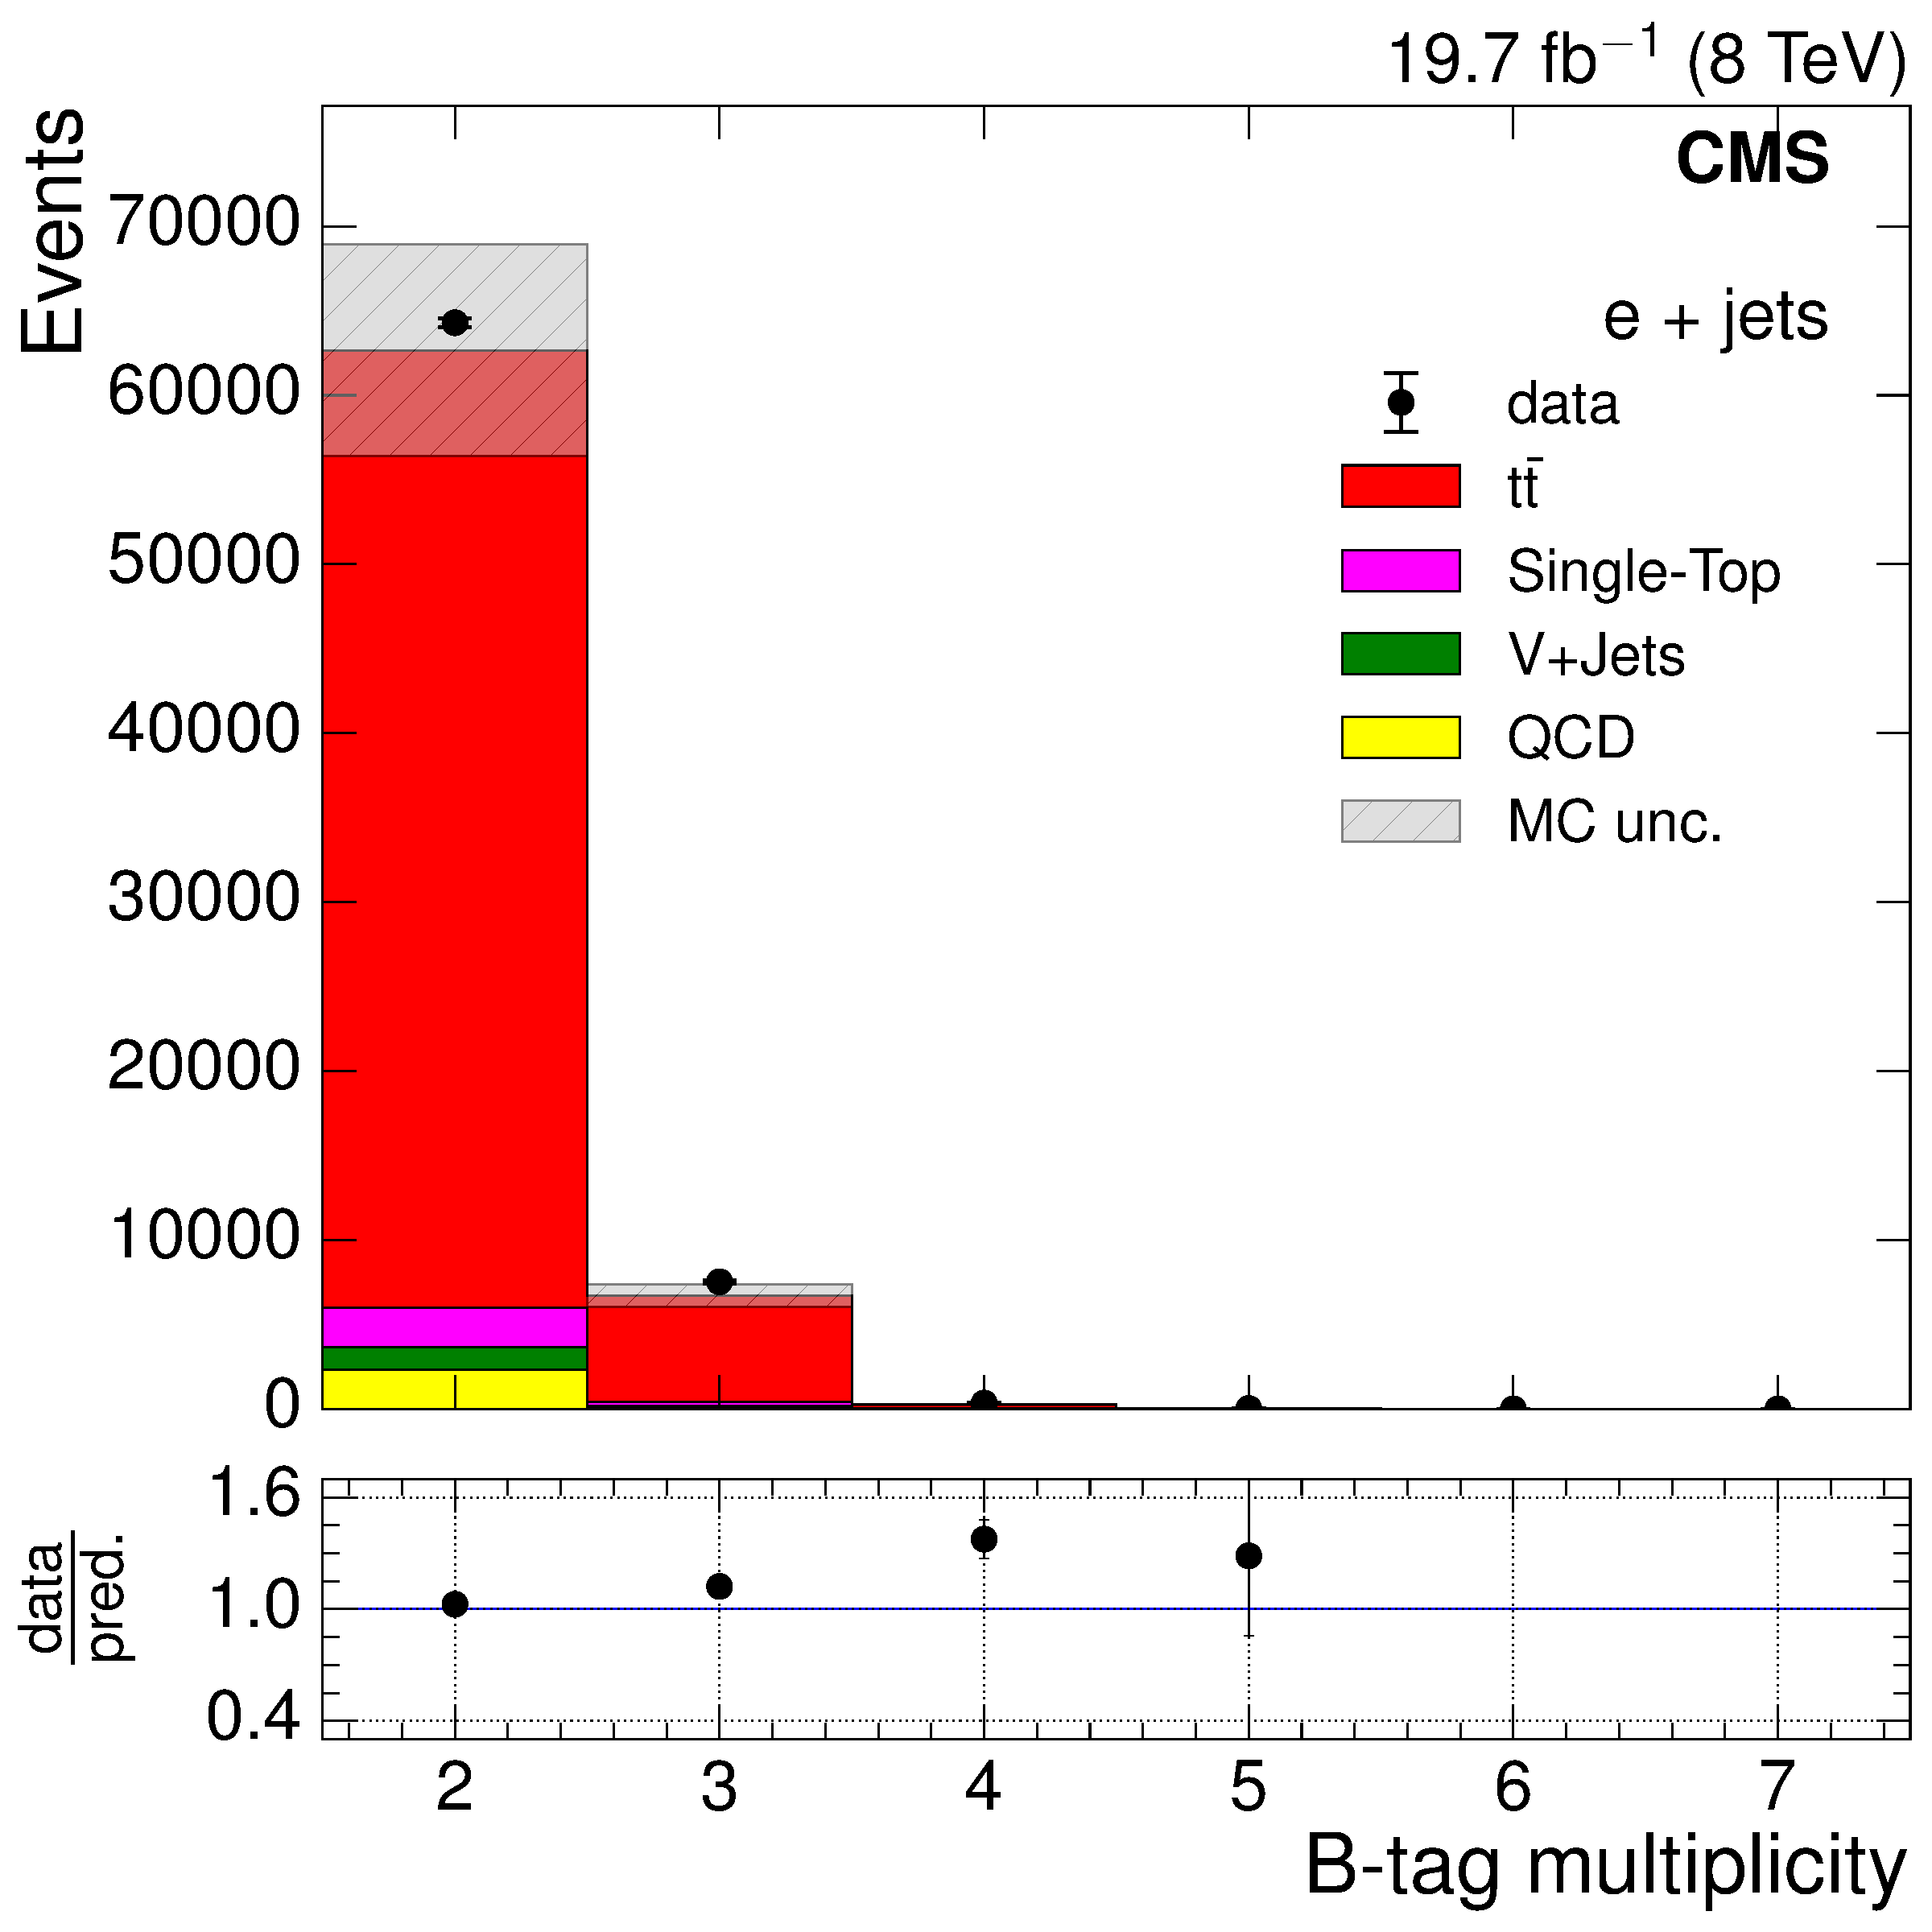
\includegraphics[width=0.48\textwidth]{Chapters/07_08_09_Analysis/Images/control_plots/before_fit/8TeV/EPlusJets_N_BJets_reweighted_with_ratio}\\
     \caption[Distributions of the number of \btags in an event in the electron+jets channel before
     and after applying \btag scale factors at $\roots=7\TeV$ and $\roots=8\TeV$.]{Distributions of
     the number of \btags in an event in the electron+jets channel before applying \btag scale factors (left)
     and after application (right) at $\roots=7\TeV$ (upper) and $\roots=8\TeV$ (lower).}
     \label{fig:nbjets_before_and_after_btag_scale_factors_electrons}
\end{figure}

%TODO: mention also not important because of fitting?

\subsection{Jet Energy Scale}
\label{sss:jet_energy_scale}
Jet energies are corrected to take into account energy coming from other sources. Level 1 (L1 Pileup)
corrections remove energy that comes from pileup collisions, Level 2 (L2 Relative) corrections remove the
dependence of jet response on $\eta$, and Level 3 (L3 Absolute) corrections correct for the jet response
dependence on \pt~\cite{Chatrchyan:2011ds}. These corrections are applied to both data and Monte Carlo
simulation events. An additional residual correction (L2L3Residual) is applied to data only for fine tuning of
the agreement between data and simulation.

Furthermore, jet energy resolution corrections are applied to simulation (known as jet smearing) to account
for the fact that jet energy resolution has been measured to be worse in data than in simulation. These PF jet
corrections are provided by the CMS JETMET Physics Object Group using 0.8\fbinv of dijet data at
$\roots=7\TeV$~\cite{Chatrchyan:2011ds} and 19.7\fbinv of dijet data at $\roots=8\TeV$~\cite{jet_res_2012}.

\subsection{Missing Transverse Energy Corrections}
\label{ss:met_corrections}

No selection criteria is placed on missing transverse energy in an event, but corrections are applied to \met
as follows. selection The adjustments to the jet energies as a result of the corrections mentioned in
Section~\ref{sss:jet_energy_scale} in turn affect the distributions of \met in the event.
Corrections known as Type-I \met corrections are applied to propagate these changes to the \met distributions
in the case of jets $\geq10\GeV$. In addition, Type-0 corrections are applied to account for pileup
interactions in the event by carrying out charged hadron subtraction (the removal of charged hadrons coming
pileup vertices). Finally, a known issue causing a roughly sinusoidal modulation of the \met distribution with
respect to $\phi$ in both simulation and data, is mitigated by applying \met $\phi$ corrections. This
correction ensures the \met distribution is independent of $\phi$, due to the rotational symmetry of
collisions around the beam axis.
 
\subsection{Trigger, Lepton ID and Isolation Efficiencies and Corrections}
\label{ss:trigger_ID_isolation_corrections}
Corrections are also required for the trigger, identification and isolation efficiencies for muons and
electrons. In the muon+jets channel, the corrections were provided by the CMS muon POG for $\roots=8\TeV$
%TODO:FINDREF (ONLY A TWIKI, WOULD THIS BE OK?)
and $\roots=7\TeV$~\cite{CMS-PAS-SMP-13-013}.

For the electron+jets channel, the corrections were provided by the CMS EGamma Physics Object Group for
$\roots=8\TeV$, %TODO:FINDREF (ONLY A TWIKI, WOULD THIS BE OK?)
however the corrections for the $\roots=7\TeV$ data were not provided and so were derived independently in
this analysis using the same tag and probe methods as used by the EGamma POG.

The 7\TeV triggers used (ElectronHad) in this analysis were not present in the 7\TeV simulation,
and so the trigger efficiency was calculated with respect to the full selection. This efficiency was then
implemented in the Monte Carlo simulation, thereby imitating the trigger. It should be noted that it is
assumed that the electron and hadron legs of the trigger are not correlated, since electrons are cleaned from
the jet collection at HLT level.

A tag and probe method~\cite{CMS:2011aa} was used to derive identification, isolation scale factors and
electron trigger efficiencies. The full reference selection was first applied with the exception of trigger,
\btagging and electron veto requirements, while in addition, a second loose electron was required. A \Z mass
constraint was placed on the two electrons in the event by requiring them to have an invariant mass of between
60\GeV and 120\GeV, thus ensuring that the pair of electrons originated from a \Z boson decay. The tight
(`tag') electron requirements were \pt$>30\GeV$, $\abseta<0.8$, relative isolation <0.1, MVA
identification$>0.9$, $d_{xy}<0.02\cm$ and reconstructed at HLT level. The loose (`probe') electron
requirements were $\pt>30\GeV$, $\abseta<2.5$ and $d_{xy}<2\cm$.

Fits were then performed, firstly of the invariant mass of all pairs of tag and probe electrons, and secondly
after applying the identification and isolation criteria to the probe electrons, to the invariant mass
distribution of pairs of tag and probe electrons in which the probe electron passed the identification and
isolation criteria. The fit was implemented in both Monte Carlo simulation and in data, and a Breit-Wigner
distribution convoluted with a Crystal Ball function is used to model the invariant mass of the tag and probe
electrons, with a falling exponential used to model the background distribution. The Breit-Wigner distribution
takes a form similar to that of a Gaussian distribution, with flatter tails~\cite{PhysRev.49.519}. The Crystal
Ball function is also based on a Gaussian distribution, but with a power-law tail to the lower end
~\cite{Oreglia,Gaiser,Skwarnicki}. Both of these functions are commonly used to model the mass peaks of
resonances. The result of this fitting procedure in data can be seen in
Figure~\ref{fig:electron_id_iso_efficiency_invariant_Z_mass_fits_data}.

\begin{figure}[hbtp]
    \centering
      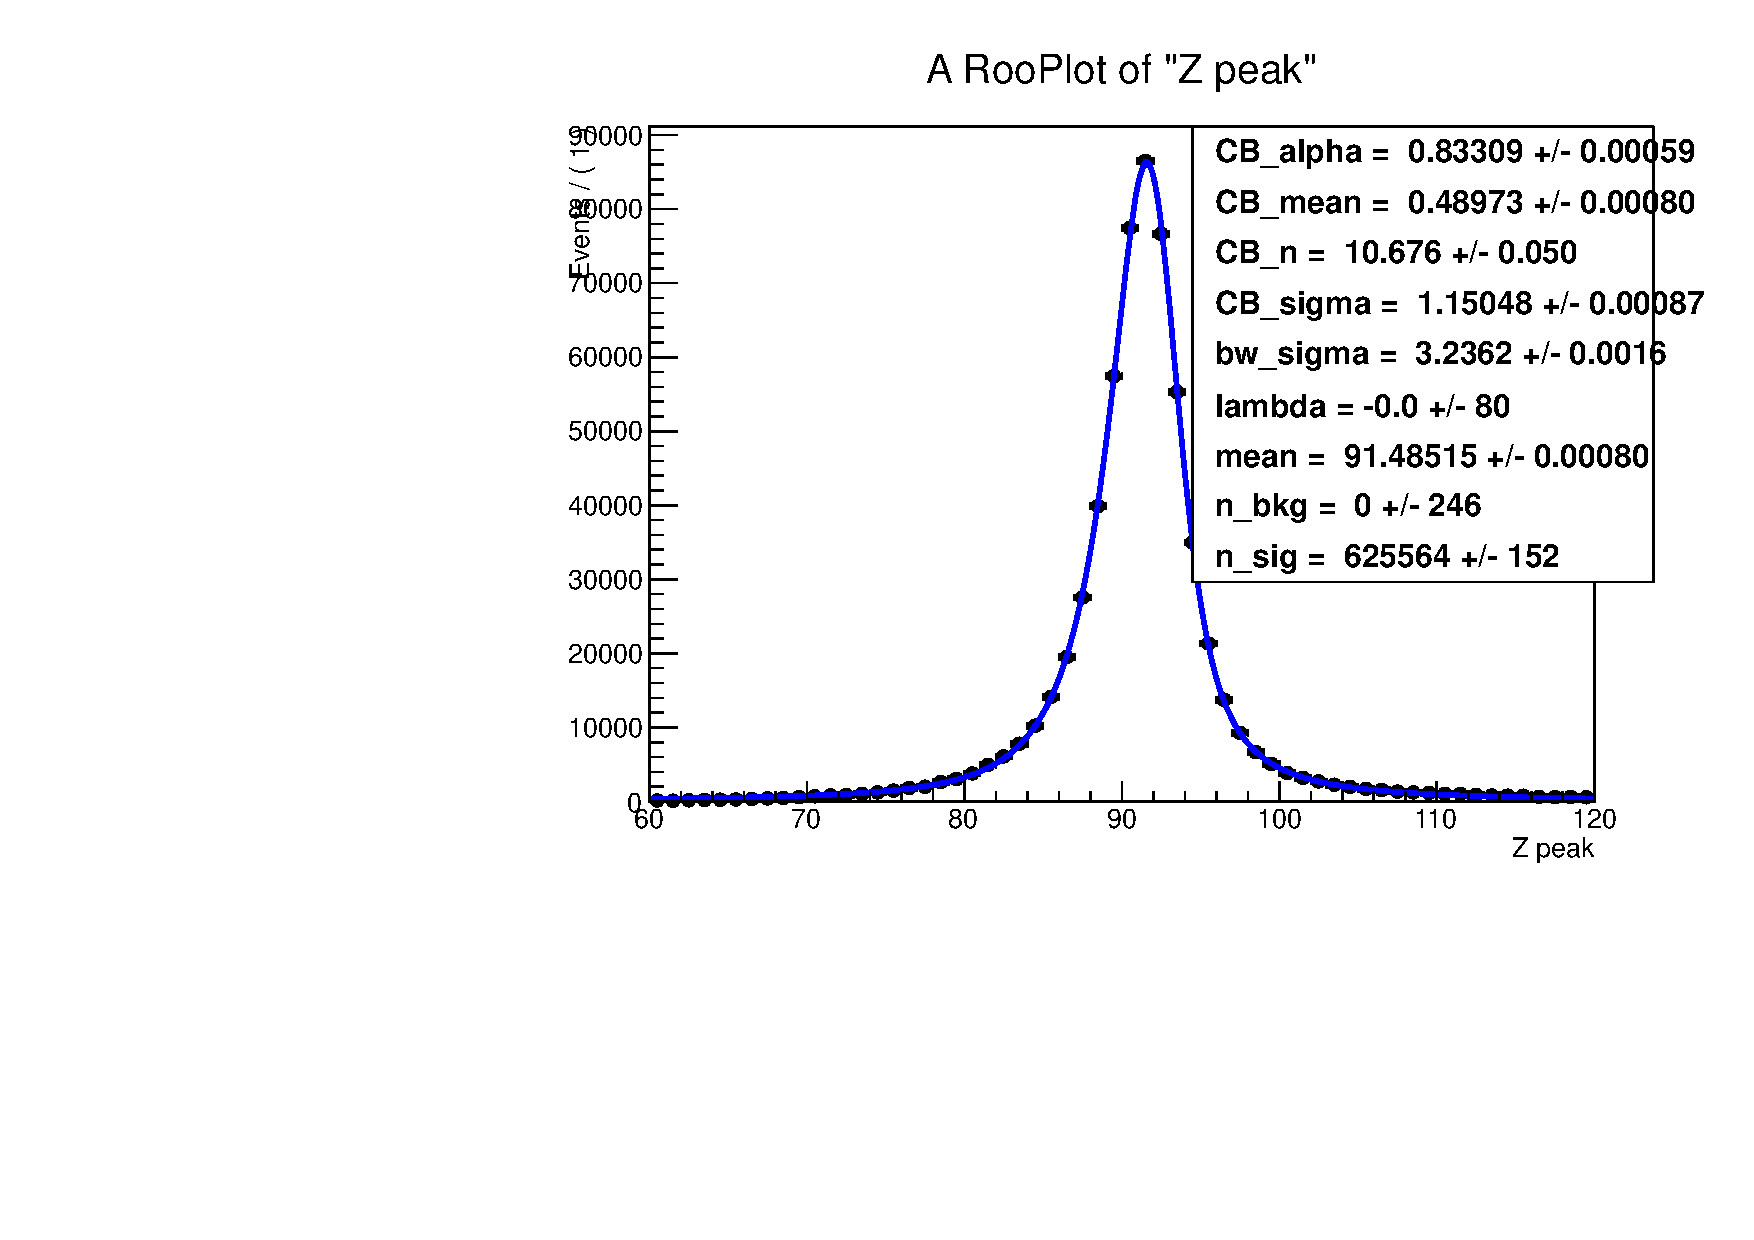
\includegraphics[width=0.48\textwidth]{Chapters/07_08_09_Analysis/Images/lepton_scale_factors/CBConvolution/electron/data/id_iso/tagProbe_total_Z_peak}\hfill
      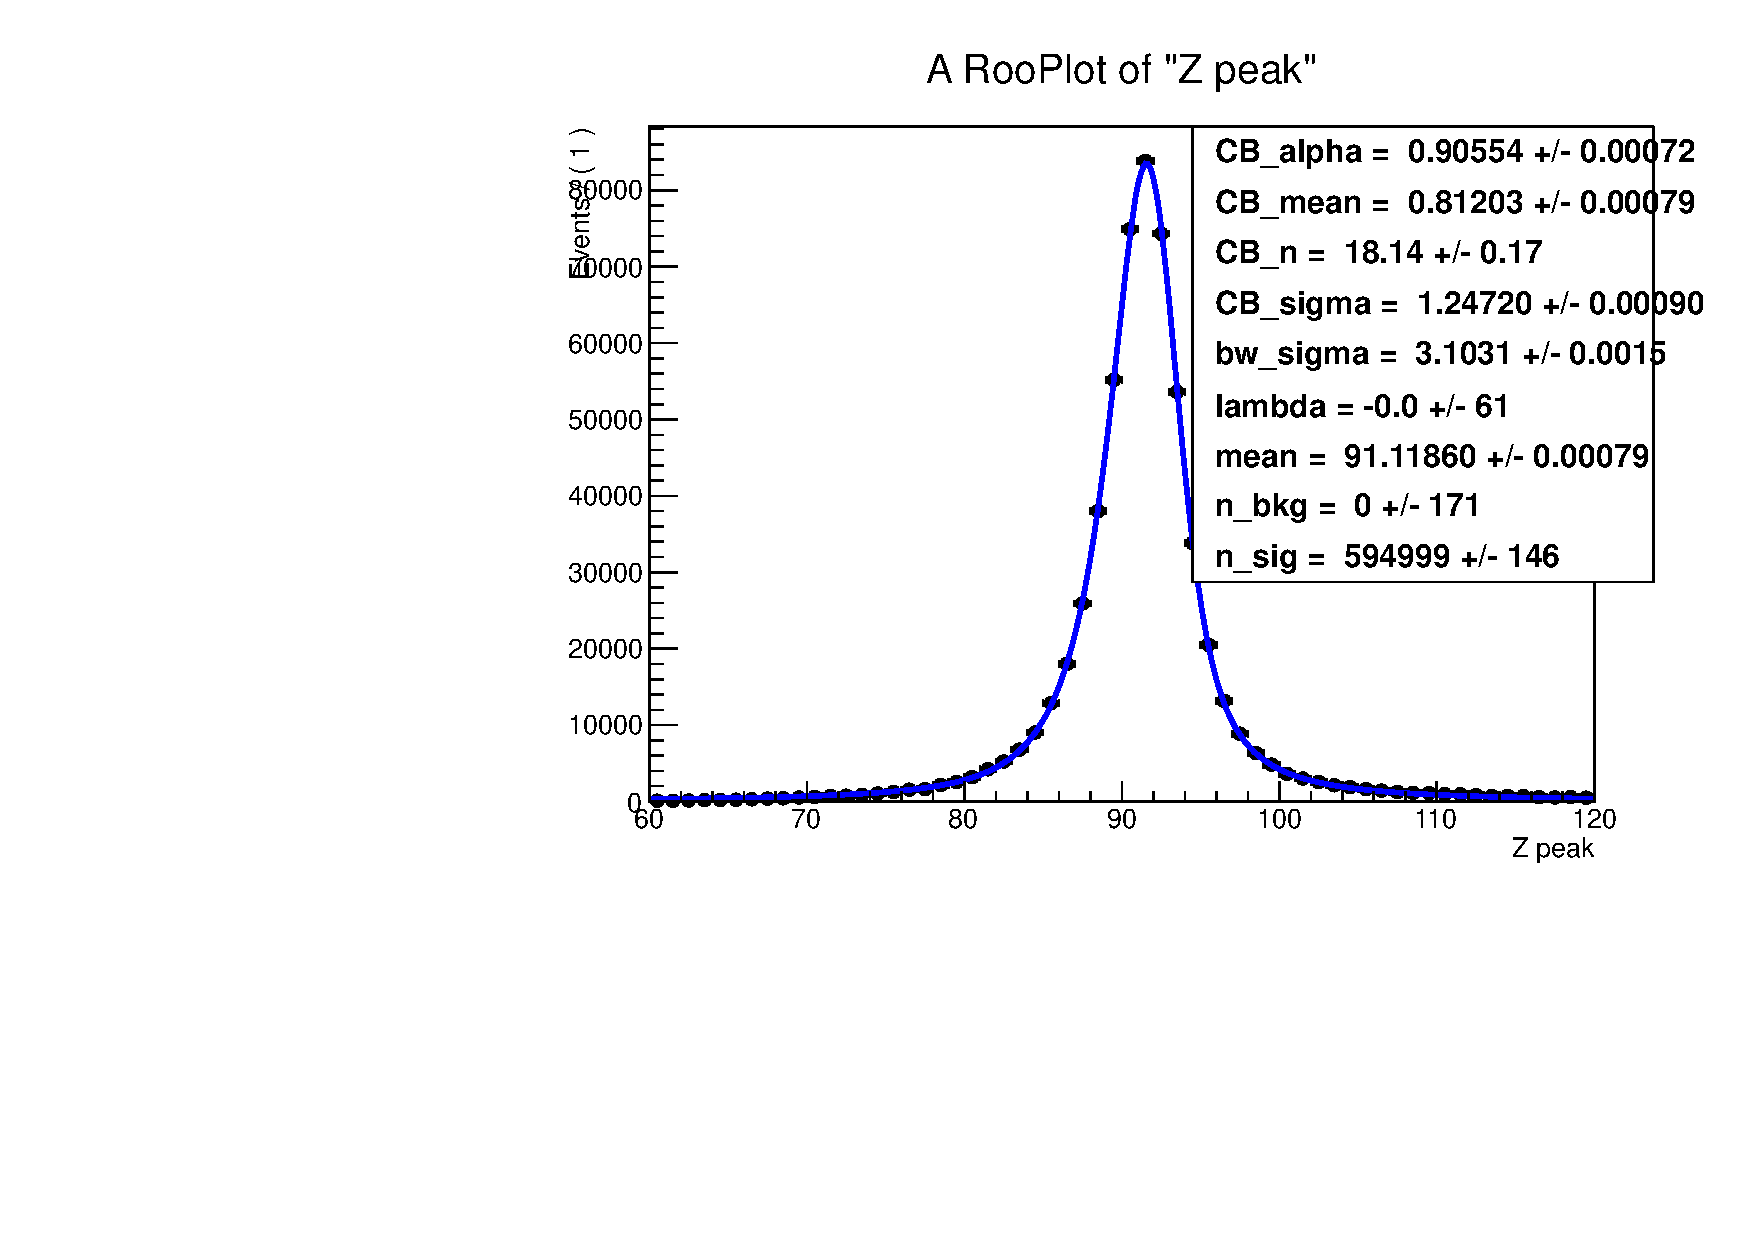
\includegraphics[width=0.48\textwidth]{Chapters/07_08_09_Analysis/Images/lepton_scale_factors/CBConvolution/electron/data/id_iso/tagProbe_passed_Z_peak}\\
     \caption[Fits of the invariant mass distribution of all tag-and-probe pairs and tag-and-probe pairs in
     which the probe satisfies the identification and isolation criteria.]{Fits of the invariant mass
     distribution of all tag-and-probe pairs (left) and tag-and-probe pairs in which the probe satisfies
     the identification and isolation criteria (right).}
     \label{fig:electron_id_iso_efficiency_invariant_Z_mass_fits_data}
\end{figure}

The efficiency of the identification and isolation process is then calculated using the numbers extracted
from the fits, in bins of \pt and $\eta$ of the probe electron, as follows:

\begin{equation}
\epsilon(\text{identification and isolation}) = \frac{N^{\text{fit}}_{\text{probe, passing}}}{N^{\text{fit}}_{\text{probe, all}}}
\end{equation}
where $N^{\text{fit}}_{\text{probe, all}}$ is the total number of events with tag and probe electrons and
$N^{\text{fit}}_{\text{probe, passing}}$ is the subset in which the probe passes identification and isolation
criteria.

The scale factor is then calculated as the ratio between the efficiencies in simulation and in data. The
efficiencies in both can be seen to be similar in Figure~\ref{fig:electron_id_iso_efficiencies_wrt_eta_pt},
leading to scale factors close to one.

\begin{figure}[hbtp]
    \centering
      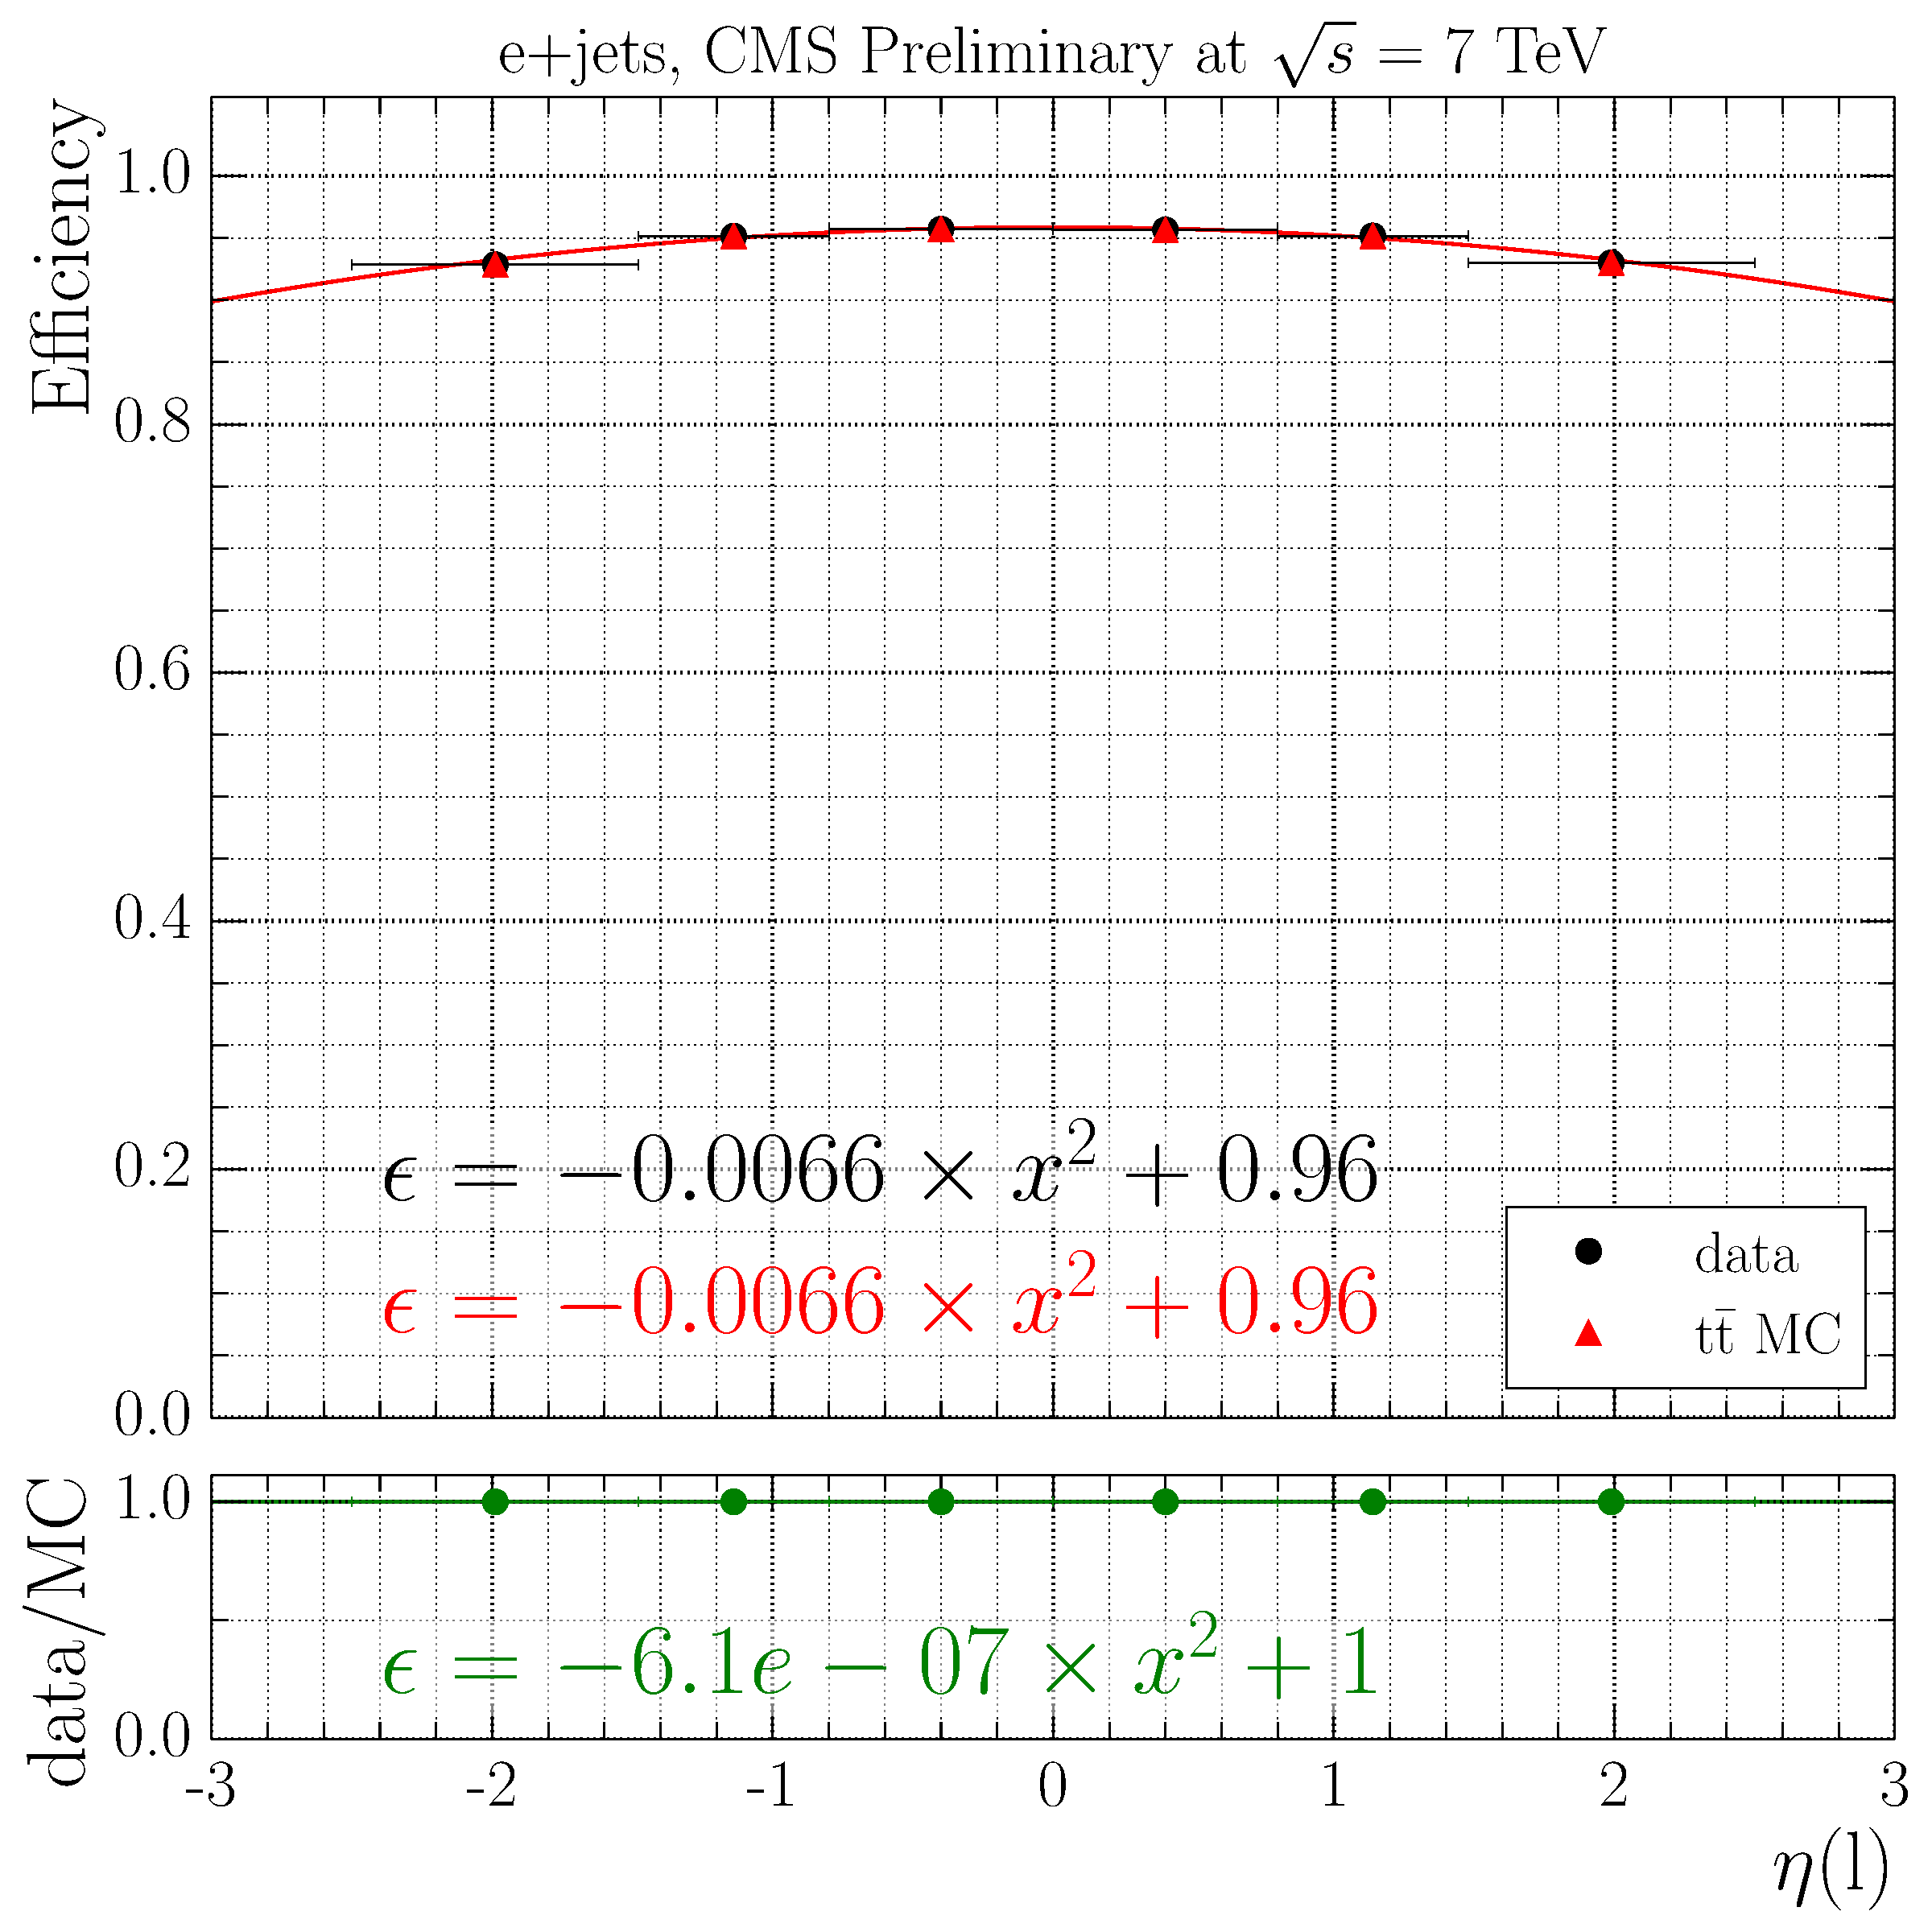
\includegraphics[width=0.48\textwidth]{Chapters/07_08_09_Analysis/Images/lepton_scale_factors/CBConvolution/electron/efficiency_eta_id_iso}\hfill
      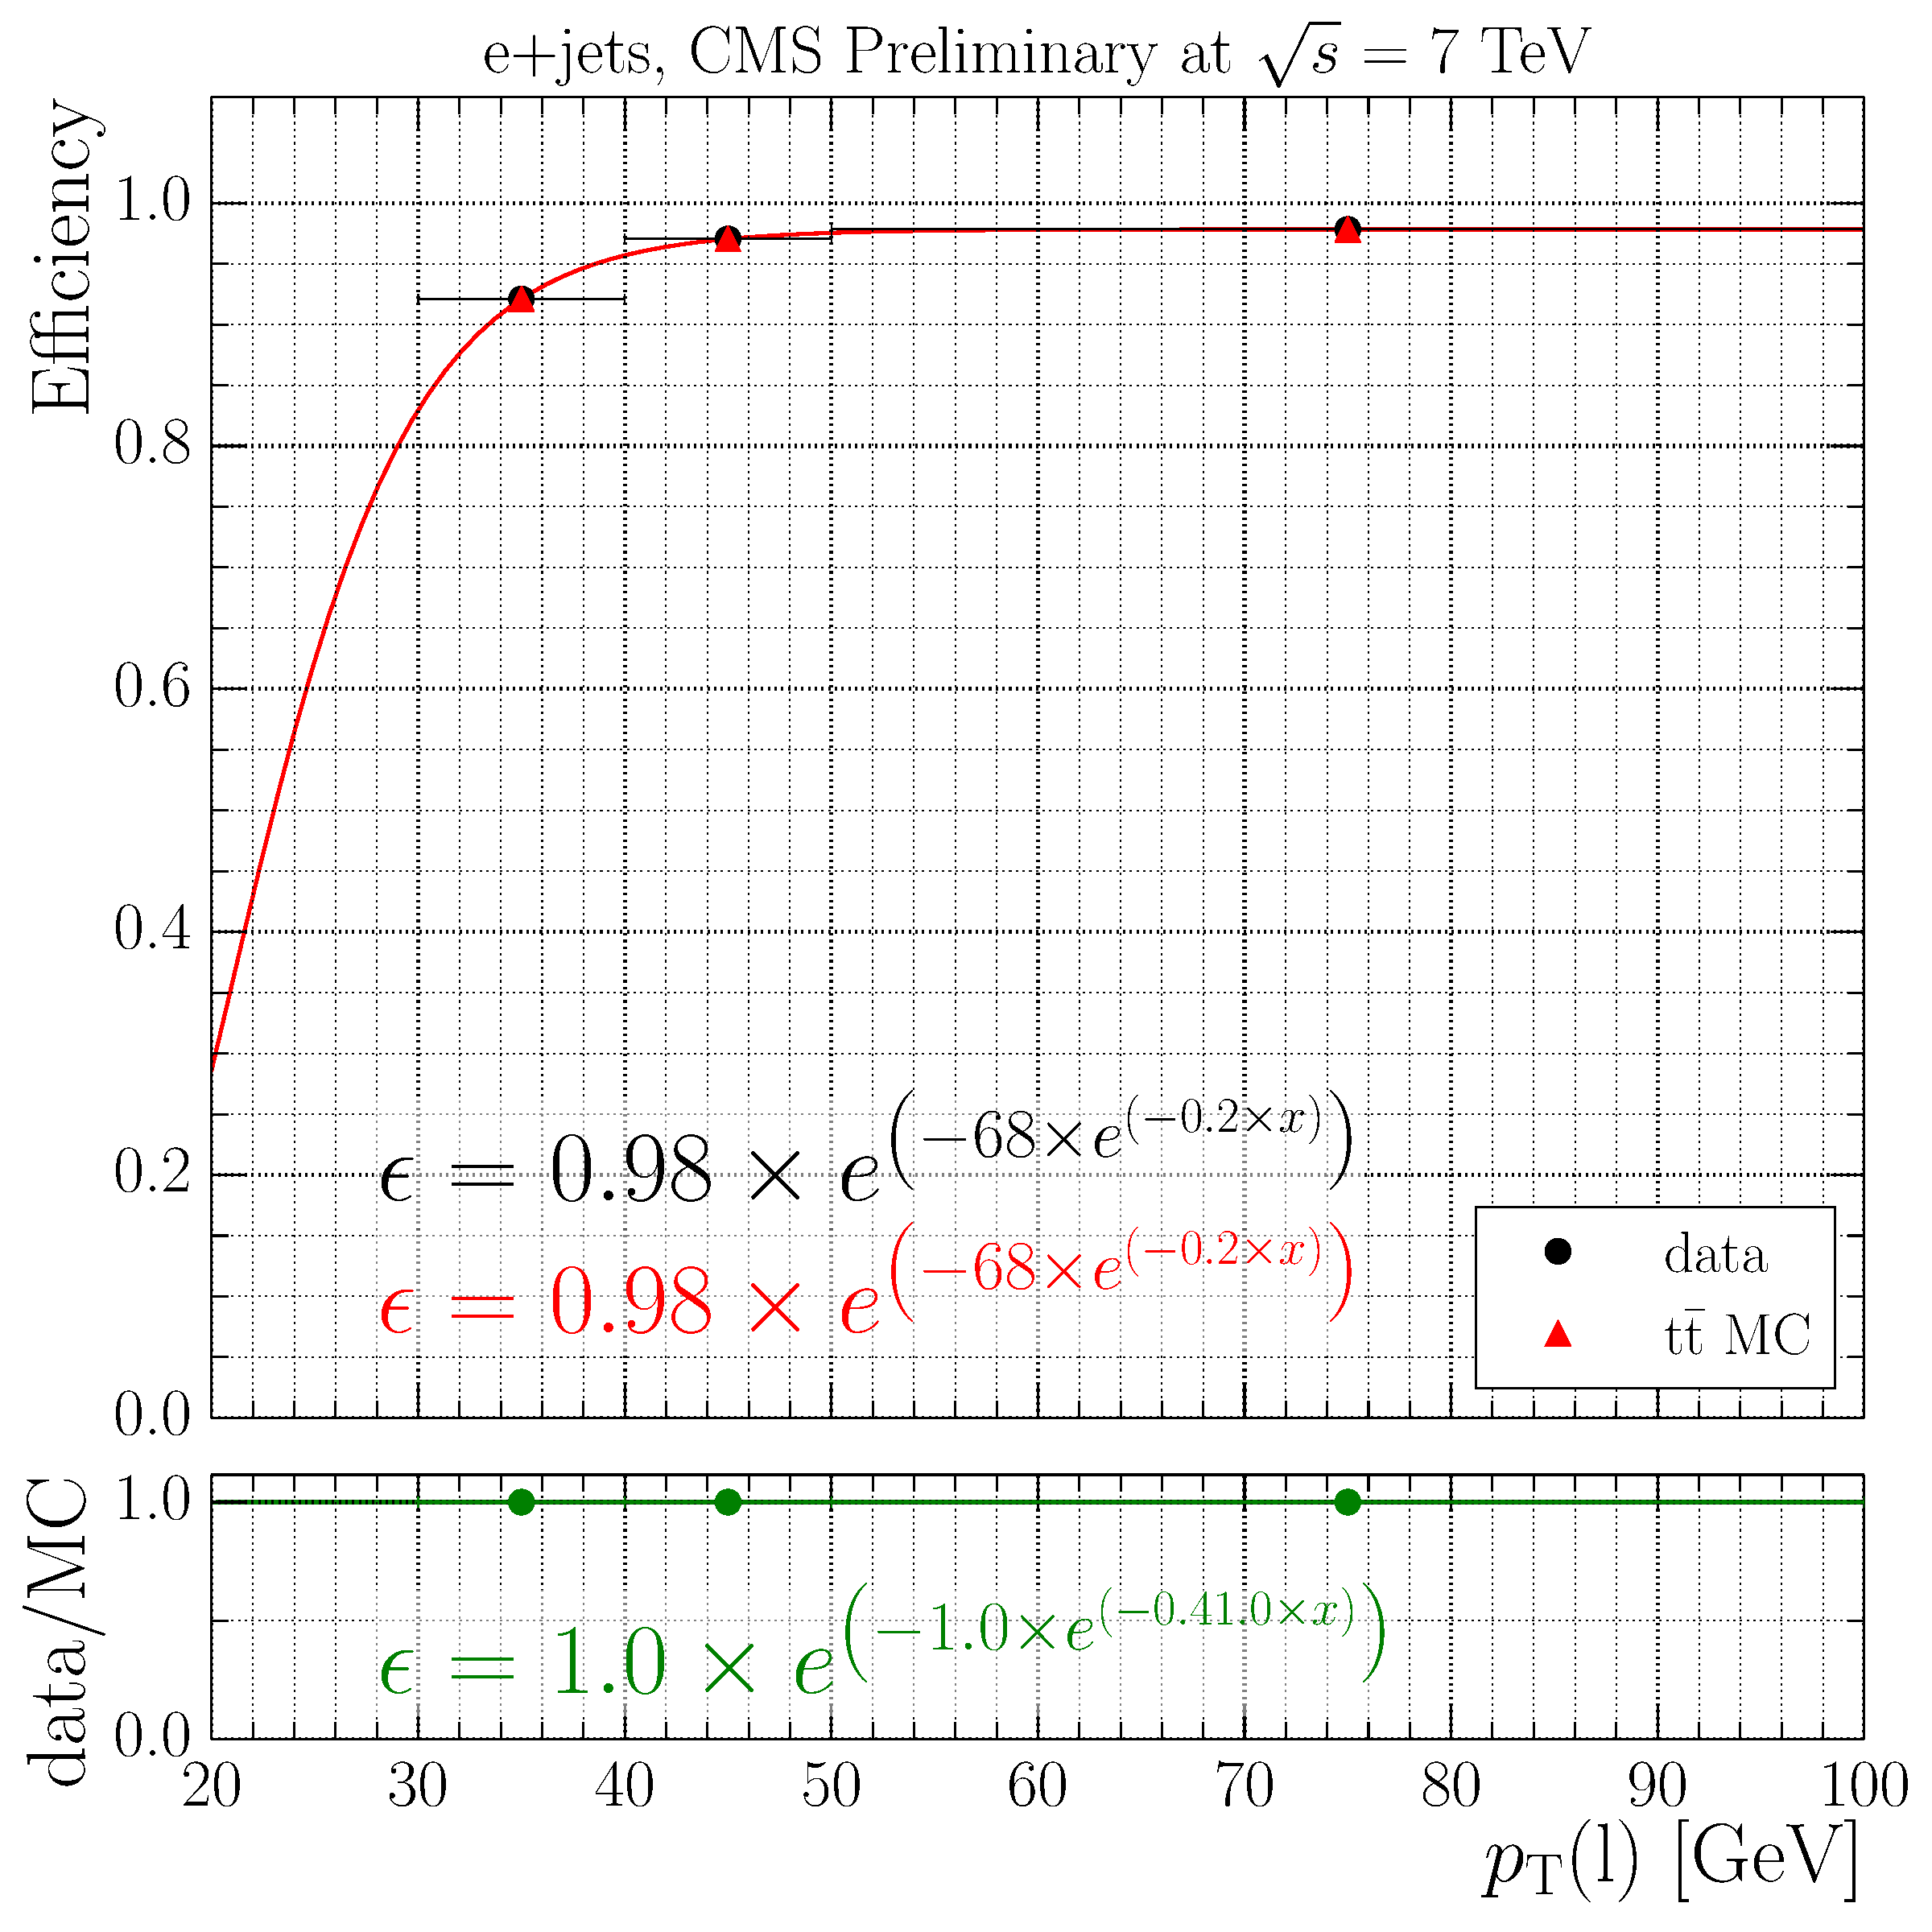
\includegraphics[width=0.48\textwidth]{Chapters/07_08_09_Analysis/Images/lepton_scale_factors/CBConvolution/electron/efficiency_pt_id_iso}
      \caption[Identification and isolation efficiencies as a function of $\eta$ and \pt in data and \ttbar
      Monte Carlo simulation.]{Identification and isolation efficiencies as a function of $\eta$ and \pt in data and \ttbar
      Monte Carlo simulation.}
     \label{fig:electron_id_iso_efficiencies_wrt_eta_pt}
\end{figure}

The efficiency of the electron part of the trigger is then similarly calculated, with respect to the
identification and isolation requirements, meaning the events passing the identification and isolation
requirements in the previous stage are then used as the baseline for the trigger efficiency. The subset of
these in which the probe electron matches a HLT electron is then used to calculate the efficiency as follows:

\begin{equation}
\epsilon(\text{trigger}) = \frac{N^{\text{fit}}_{\text{probe, matching HLT}}}{N^{\text{fit}}_{\text{probe,identification and isolation}}}
\label{eq:electron_leg_efficiency}
\end{equation}
where $N^{\text{fit}}_{\text{probe,identification and isolation}}$ is the number of
events passing from equation~\ref{eq:electron_leg_efficiency} and $N^{\text{fit}}_{\text{probe, matching
HLT}}$ is the subset in which the probe is matched to an HLT electron object.

In order to calculate the efficiency of the hadron leg of the trigger, the full selection with only the
electron part of the trigger and without \btagging, applied to the SingleElectron dataset, is taken as the
baseline. The number of these events passing the hadronic leg of the trigger is then used to calculate the
hadronic leg efficiency as follows:

\begin{equation}
\epsilon(\text{hadron leg}) = \frac{N_{\text{hadron leg, passing}}}{N_{\text{passing selection}}}
\end{equation}
where $N_{\text{passing selection}}$ is the number of events passing the baseline selection with
the electron leg of the trigger and no \btagging requirements, and $N_{\text{hadron leg, passing}}$ is the
subset in which the hadron leg of the trigger is satisfied.

The scale factors are produced in bins of \pt and $\eta$ of the fourth most energetic jet, since this is the
lowest energy jet that is selected. Parametrising as a function of higher energy jets would lead to a bias
towards high efficiencies as the trigger will have a higher efficiency at higher jet energies.

Equivalent fit and efficiency plots for the trigger are included in
Figures~\ref{fig:electron_trigger_efficiency_invariant_Z_mass_fits} and
\ref{fig:electron_trigger_efficiencies_wrt_eta_pt} in Appendix~\ref{as:data_monte_carlo_corrections}.

\chapter{Differential Cross Sections: Fitting, Unfolding and Measurement}
\label{c:Differential_Cross_Section:fitting_unfolding_and_measurement}

% \section{Introduction}
% \label:{s:analysis2_introduction}
% Following event selection it is important to perform a comparison of simulation to data to verify that the
% processes modelled as backgrounds 

\section{Data-MC Comparison}
\label{ss:data-mc_comparison}
Following the full event selection, the simulated events are scaled to match the luminosity of the data using
the scale factor:
\begin{equation}
  S = \frac{{\cal L} \times  \sigma}{N_{\rm processed}}
\end{equation}
where $N_{\rm processed}$ is the total number of events processed for each Monte Carlo sample and $\sigma$ is
the production cross section of each process. The numbers of events passing each selection step in data and
in Monte Carlo simulation, after scaling to the measured luminosities, are shown for both the electron+jets
and muon+jets channels at $\roots=7\TeV$ in Table~\ref{tab:cut_flow_7TeV}, and at $\roots=8\TeV$ in
Table~\ref{tab:cut_flow_8TeV}.

\begin{table}
  \centering
   \caption{Expected and observed event yields at several stages of the electron+jets selection (upper) and
   the muon+jets channel selection (lower) at \roots=7\TeV.}
%   The figures in italics are data-driven estimates of QCD background.}
    \label{tab:cut_flow_7TeV}
    \resizebox{\columnwidth}{!} {
    \begin{tabular}{lrrrrrrr}
    \hline
    \hline
	Selection step & \ttbar + jets & \WpJets & \ZpJets & Single-Top & QCD & Sum MC & Data \\
	\hline
	Preselection  &  $248837 \pm 131$ &  $296487 \pm 255$ &  $87027 \pm 237$ &  $26397 \pm 43$ &  $24578753 \pm 81165$ &  $25237503 \pm 81166$ &  4928736 \\ 
	Event cleaning/HLT  &  $248712 \pm 131$ &  $296343 \pm 255$ &  $86964 \pm 237$ &  $26385 \pm 43$ &  $24574668 \pm 81161$ &  $25233075 \pm 81162$ &  1103841 \\ 
	One isolated electron  &  $70973 \pm 69$ &  $91618 \pm 132$ &  $26311 \pm 122$ &  $5355 \pm 17$ &  $263313 \pm 6601$ &  $457572 \pm 6604$ &  299020 \\ 
	Muon veto  &  $67163 \pm 67$ &  $91581 \pm 132$ &  $26196 \pm 122$ &  $5269 \pm 17$ &  $263195 \pm 6601$ &  $453405 \pm 6604$ &  295961 \\ 
	Dilepton veto  &  $66336 \pm 67$ &  $91559 \pm 132$ &  $20560 \pm 107$ &  $5251 \pm 17$ &  $263183 \pm 6601$ &  $446892 \pm 6603$ &  289456 \\ 
	Conversion veto  &  $64497 \pm 66$ &  $87866 \pm 130$ &  $19671 \pm 105$ &  $5106 \pm 16$ &  $174315 \pm 5761$ &  $351458 \pm 5763$ &  243472 \\ 
	$\geq 1$ jets  &  $64497 \pm 66$ &  $87866 \pm 130$ &  $19671 \pm 105$ &  $5106 \pm 16$ &  $174315 \pm 5761$ &  $351457 \pm 5763$ &  243471 \\ 
	$\geq 2$ jets  &  $64489 \pm 66$ &  $87789 \pm 130$ &  $19633 \pm 105$ &  $5104 \pm 16$ &  $173680 \pm 5748$ &  $350697 \pm 5750$ &  243446 \\ 
	$\geq 3$ jets  &  $63514 \pm 65$ &  $82167 \pm 123$ &  $18188 \pm 101$ &  $4912 \pm 16$ &  $126305 \pm 4416$ &  $295088 \pm 4420$ &  236124 \\ 
	$\geq 4$ jets  &  $35285 \pm 48$ &  $17935 \pm 42$ &  $3618 \pm 45$ &  $1461 \pm 8$ &  $21354 \pm 1507$ &  $79656 \pm 1509$ &  71414 \\ 
	$\geq 1$ b-tagged jets  &  $29777 \pm 44$ &  $2764 \pm 17$ &  $562 \pm 17$ &  $1160 \pm 7$ &  $3601 \pm 513$ &  $37864 \pm 516$ &  34671 \\ 
	$\geq 2$ b-tagged jets  &  $13777 \pm 30$ &  $326 \pm 4$ &  $76 \pm 6$ &  $434 \pm 4$ &  $590 \pm 220$ &  $15205 \pm 222$ &  13792 \\ 
	\hline
	\hline
	Selection step & \ttbar + jets & \WpJets & \ZpJets & Single-Top & QCD & Sum MC & Data \\
	\hline
	Preselection  &  $248280 \pm 131$ &  $296599 \pm 255$ &  $87128 \pm 237$ &  $26362 \pm 43$ &  $18658866 \pm 41697$ &  $19317237 \pm 41699$ &  4201249 \\ 
	Event cleaning/HLT  &  $248155 \pm 131$ &  $296455 \pm 255$ &  $87065 \pm 237$ &  $26350 \pm 43$ &  $18655836 \pm 41690$ &  $19313864 \pm 41692$ &  444679 \\ 
	One isolated muon  &  $74418 \pm 71$ &  $93902 \pm 132$ &  $22774 \pm 115$ &  $5724 \pm 19$ &  $45516 \pm 2160$ &  $242336 \pm 2168$ &  206738 \\ 
	Second muon veto  &  $73036 \pm 70$ &  $93893 \pm 132$ &  $14109 \pm 89$ &  $5690 \pm 19$ &  $44741 \pm 2153$ &  $231470 \pm 2161$ &  194980 \\ 
	Electron veto  &  $69681 \pm 69$ &  $93852 \pm 132$ &  $14020 \pm 89$ &  $5615 \pm 19$ &  $44666 \pm 2153$ &  $227835 \pm 2160$ &  192335 \\ 
	$\geq 1$ jets  &  $69680 \pm 69$ &  $93851 \pm 132$ &  $14020 \pm 89$ &  $5615 \pm 19$ &  $44648 \pm 2153$ &  $227816 \pm 2160$ &  192335 \\ 
	$\geq 2$ jets  &  $69675 \pm 69$ &  $93791 \pm 132$ &  $14007 \pm 89$ &  $5613 \pm 19$ &  $43404 \pm 2139$ &  $226492 \pm 2146$ &  192310 \\ 
	$\geq 3$ jets  &  $69054 \pm 68$ &  $89508 \pm 126$ &  $13186 \pm 86$ &  $5455 \pm 18$ &  $14627 \pm 1059$ &  $191831 \pm 1072$ &  186061 \\ 
	$\geq 4$ jets  &  $38222 \pm 50$ &  $19234 \pm 42$ &  $2707 \pm 38$ &  $1573 \pm 8$ &  $2028 \pm 242$ &  $63766 \pm 254$ &  54684 \\ 
	$\geq 1$ b-tagged jets  &  $32268 \pm 46$ &  $2965 \pm 16$ &  $463 \pm 15$ &  $1250 \pm 7$ &  $873 \pm 148$ &  $37821 \pm 157$ &  30852 \\ 
	$\geq 2$ b-tagged jets  &  $15016 \pm 30$ &  $355 \pm 5$ &  $60 \pm 5$ &  $468 \pm 4$ &  $180 \pm 48$ &  $16081 \pm 58$ &  13128 \\ 
	\hline
	\hline
	\end{tabular}
	}
\end{table}

%==================================================
%Selection step & \ttbar + jets & \Wpjets & \Zpjets & Single-Top & QCD & Sum MC & Data \\
%Preselection  &  $248837 \pm 131$ &  $296487 \pm 255$ &  $87027 \pm 237$ &  $26397 \pm 43$ &  $24578753 \pm
% 81165$ &  $25237503 \pm 81166$ &  4928736 \\
%Event cleaning/HLT  &  $248712 \pm 131$ &  $296343 \pm 255$ &  $86964 \pm 237$ &  $26385 \pm 43$ &  $24574668
% \pm 81161$ &  $25233075 \pm 81162$ &  1103841 \\
%One isolated electron  &  $70973 \pm 69$ &  $91618 \pm 132$ &  $26311 \pm 122$ &  $5355 \pm 17$ &  $263313
% \pm 6601$ &  $457572 \pm 6604$ &  299020 \\
%Muon veto  &  $67163 \pm 67$ &  $91581 \pm 132$ &  $26196 \pm 122$ &  $5269 \pm 17$ &  $263195 \pm 6601$ & 
% $453405 \pm 6604$ &  295961 \\
%Dilepton veto  &  $66336 \pm 67$ &  $91559 \pm 132$ &  $20560 \pm 107$ &  $5251 \pm 17$ &  $263183 \pm 6601$
% &  $446892 \pm 6603$ &  289456 \\
%Conversion veto  &  $64497 \pm 66$ &  $87866 \pm 130$ &  $19671 \pm 105$ &  $5106 \pm 16$ &  $174315 \pm
% 5761$ &  $351458 \pm 5763$ &  243472 \\
%$\geq 1$ jets  &  $64497 \pm 66$ &  $87866 \pm 130$ &  $19671 \pm 105$ &  $5106 \pm 16$ &  $174315 \pm 5761$
% &  $351457 \pm 5763$ &  243471 \\
%$\geq 2$ jets  &  $64489 \pm 66$ &  $87789 \pm 130$ &  $19633 \pm 105$ &  $5104 \pm 16$ &  $173680 \pm 5748$
% &  $350697 \pm 5750$ &  243446 \\
%$\geq 3$ jets  &  $63514 \pm 65$ &  $82167 \pm 123$ &  $18188 \pm 101$ &  $4912 \pm 16$ &  $126305 \pm 4416$
% &  $295088 \pm 4420$ &  236124 \\
%$\geq 4$ jets  &  $35285 \pm 48$ &  $17935 \pm 42$ &  $3618 \pm 45$ &  $1461 \pm 8$ &  $21354 \pm 1507$ & 
% $79656 \pm 1509$ &  71414 \\
%$\geq 1$ b-tagged jets  &  $29777 \pm 44$ &  $2764 \pm 17$ &  $562 \pm 17$ &  $1160 \pm 7$ &  $3601 \pm 513$
% &  $37864 \pm 516$ &  34671 \\
%$\geq 2$ b-tagged jets  &  $13777 \pm 30$ &  $326 \pm 4$ &  $76 \pm 6$ &  $434 \pm 4$ &  $590 \pm 220$ & 
% $15205 \pm 222$ &  13792 \\
% ==================================================
% Selection step & \ttbar + jets & \Wpjets & \Zpjets & Single-Top & QCD & Sum MC & Data \\
% Preselection  &  $248280 \pm 131$ &  $296599 \pm 255$ &  $87128 \pm 237$ &  $26362 \pm 43$ &  $18658866 \pm 41697$ &  $19317237 \pm 41699$ &  4201249 \\ 
% Event cleaning/HLT  &  $248155 \pm 131$ &  $296455 \pm 255$ &  $87065 \pm 237$ &  $26350 \pm 43$ &  $18655836 \pm 41690$ &  $19313864 \pm 41692$ &  444679 \\ 
% One isolated muon  &  $74418 \pm 71$ &  $93902 \pm 132$ &  $22774 \pm 115$ &  $5724 \pm 19$ &  $45516 \pm 2160$ &  $242336 \pm 2168$ &  206738 \\ 
% Second muon veto  &  $73036 \pm 70$ &  $93893 \pm 132$ &  $14109 \pm 89$ &  $5690 \pm 19$ &  $44741 \pm 2153$ &  $231470 \pm 2161$ &  194980 \\ 
% Electron veto  &  $69681 \pm 69$ &  $93852 \pm 132$ &  $14020 \pm 89$ &  $5615 \pm 19$ &  $44666 \pm 2153$ &  $227835 \pm 2160$ &  192335 \\ 
% $\geq 1$ jets  &  $69680 \pm 69$ &  $93851 \pm 132$ &  $14020 \pm 89$ &  $5615 \pm 19$ &  $44648 \pm 2153$ &  $227816 \pm 2160$ &  192335 \\ 
% $\geq 2$ jets  &  $69675 \pm 69$ &  $93791 \pm 132$ &  $14007 \pm 89$ &  $5613 \pm 19$ &  $43404 \pm 2139$ &  $226492 \pm 2146$ &  192310 \\ 
% $\geq 3$ jets  &  $69054 \pm 68$ &  $89508 \pm 126$ &  $13186 \pm 86$ &  $5455 \pm 18$ &  $14627 \pm 1059$ &  $191831 \pm 1072$ &  186061 \\ 
% $\geq 4$ jets  &  $38222 \pm 50$ &  $19234 \pm 42$ &  $2707 \pm 38$ &  $1573 \pm 8$ &  $2028 \pm 242$ &  $63766 \pm 254$ &  54684 \\ 
% $\geq 1$ b-tagged jets  &  $32268 \pm 46$ &  $2965 \pm 16$ &  $463 \pm 15$ &  $1250 \pm 7$ &  $873 \pm 148$ &  $37821 \pm 157$ &  30852 \\ 
% $\geq 2$ b-tagged jets  &  $15016 \pm 30$ &  $355 \pm 5$ &  $60 \pm 5$ &  $468 \pm 4$ &  $180 \pm 48$ &  $16081 \pm 58$ &  13128 \\ 

\begin{table}
  \centering
   \caption{Expected and observed event yields at several stages of the electron+jets selection (upper) and
   the muon+jets selection (lower) at \roots=8\TeV.}
%   The figures in italics are data-driven estimates of QCD background.}
    \label{tab:cut_flow_8TeV}
    \resizebox{\columnwidth}{!} {
    \begin{tabular}{lrrrrrrr}
    \hline
    \hline
	Selection step & \ttbar + jets & \WpJets & \ZpJets & Single-Top & QCD & Sum MC & Data \\
	\hline
	Preselection  &  $1389239 \pm 1071$ &  $1748404 \pm 1149$ &  $385132 \pm 236$ &  $170598 \pm 265$ &  $131270649 \pm 477929$ &  $134964023 \pm 477932$ &  13219192 \\ 
	Event cleaning/HLT  &  $376950 \pm 547$ &  $493785 \pm 573$ &  $143253 \pm 138$ &  $35559 \pm 122$ &  $3844108 \pm 83191$ &  $4893656 \pm 83195$ &  5952438 \\ 
	One isolated electron  &  $335908 \pm 515$ &  $427471 \pm 520$ &  $95501 \pm 111$ &  $31520 \pm 115$ &  $554050 \pm 27723$ &  $1444453 \pm 27733$ &  1754243 \\ 
	Muon veto  &  $316823 \pm 500$ &  $427354 \pm 520$ &  $95069 \pm 111$ &  $30820 \pm 113$ &  $553991 \pm 27723$ &  $1424058 \pm 27733$ &  1733585 \\ 
	Dilepton veto  &  $312321 \pm 497$ &  $427247 \pm 520$ &  $70836 \pm 96$ &  $30648 \pm 113$ &  $553952 \pm 27723$ &  $1395005 \pm 27733$ &  1692425 \\ 
	Conversion veto  &  $304300 \pm 490$ &  $411661 \pm 510$ &  $68005 \pm 94$ &  $29849 \pm 111$ &  $309968 \pm 20284$ &  $1123785 \pm 20297$ &  1447105 \\ 
	$\geq 1$ jets  &  $304300 \pm 490$ &  $411658 \pm 510$ &  $68005 \pm 94$ &  $29849 \pm 111$ &  $309968 \pm 20284$ &  $1123781 \pm 20297$ &  1447105 \\ 
	$\geq 2$ jets  &  $304264 \pm 490$ &  $411028 \pm 510$ &  $67901 \pm 94$ &  $29834 \pm 111$ &  $307974 \pm 20200$ &  $1121003 \pm 20213$ &  1446970 \\ 
	$\geq 3$ jets  &  $299232 \pm 486$ &  $372483 \pm 472$ &  $61904 \pm 87$ &  $28518 \pm 109$ &  $226054 \pm 16034$ &  $988193 \pm 16049$ &  1251530 \\ 
	$\geq 4$ jets  &  $172557 \pm 369$ &  $76326 \pm 175$ &  $13484 \pm 35$ &  $9524 \pm 64$ &  $43901 \pm 4145$ &  $315795 \pm 4165$ &  361692 \\ 
	$\geq 1$ b-tagged jets  &  $142836 \pm 332$ &  $10417 \pm 65$ &  $2019 \pm 13$ &  $7296 \pm 55$ &  $8705 \pm 1812$ &  $171275 \pm 1845$ &  181705 \\ 
	$\geq 2$ b-tagged jets  &  $63233 \pm 215$ &  $1114 \pm 21$ &  $291 \pm 4$ &  $2566 \pm 32$ &  $2427 \pm 1660$ &  $69632 \pm 1675$ &  72176 \\ 
	\hline
	\hline
	Selection step & \ttbar + jets & \WpJets & \ZpJets & Single-Top & QCD & Sum MC & Data \\
	\hline
	Preselection  &  $1400798 \pm 1080$ &  $1765900 \pm 1159$ &  $389320 \pm 239$ &  $171677 \pm 266$ &  $104820777 \pm 238065$ &  $108548474 \pm 238070$ &  20815265 \\ 
	Event cleaning/HLT  &  $469828 \pm 622$ &  $669486 \pm 711$ &  $153379 \pm 147$ &  $46228 \pm 141$ &  $1673119 \pm 33684$ &  $3012042 \pm 33698$ &  3166723 \\ 
	One isolated muon  &  $385092 \pm 562$ &  $496720 \pm 582$ &  $92752 \pm 111$ &  $37012 \pm 126$ &  $89801 \pm 6391$ &  $1101379 \pm 6444$ &  1373749 \\ 
	Second muon veto  &  $377038 \pm 556$ &  $496660 \pm 582$ &  $54606 \pm 85$ &  $36705 \pm 126$ &  $89060 \pm 6380$ &  $1054070 \pm 6433$ &  1292713 \\ 
	Electron veto  &  $358624 \pm 542$ &  $496506 \pm 582$ &  $54260 \pm 85$ &  $36049 \pm 124$ &  $89037 \pm 6380$ &  $1034478 \pm 6431$ &  1274884 \\ 
	$\geq 1$ jets  &  $358624 \pm 542$ &  $496498 \pm 582$ &  $54259 \pm 85$ &  $36049 \pm 124$ &  $89037 \pm 6380$ &  $1034470 \pm 6431$ &  1274884 \\ 
	$\geq 2$ jets  &  $358592 \pm 542$ &  $495658 \pm 581$ &  $54186 \pm 85$ &  $36029 \pm 124$ &  $88048 \pm 6354$ &  $1032515 \pm 6405$ &  1274817 \\ 
	$\geq 3$ jets  &  $354271 \pm 539$ &  $448652 \pm 534$ &  $49426 \pm 78$ &  $34498 \pm 122$ &  $34560 \pm 2810$ &  $921409 \pm 2914$ &  1138923 \\ 
	$\geq 4$ jets  &  $202771 \pm 407$ &  $90874 \pm 199$ &  $10999 \pm 32$ &  $11233 \pm 71$ &  $8003 \pm 1304$ &  $323883 \pm 1383$ &  351087 \\ 
	$\geq 1$ b-tagged jets  &  $168125 \pm 367$ &  $12499 \pm 73$ &  $1715 \pm 12$ &  $8660 \pm 61$ &  $4252 \pm 1036$ &  $195253 \pm 1104$ &  197025 \\ 
	$\geq 2$ b-tagged jets  &  $74995 \pm 238$ &  $1367 \pm 23$ &  $229 \pm 4$ &  $3023 \pm 35$ &  $527 \pm 410$ &  $80143 \pm 476$ &  81047 \\
	\hline
	\hline
    \end{tabular}
    }
\end{table}

% ==================================================
% Selection step & \ttbar + jets & W + jets & Z + jets & Single-Top & QCD & Sum MC & Data \\
% Preselection  &  $1389239 \pm 1071$ &  $1748404 \pm 1149$ &  $385132 \pm 236$ &  $170598 \pm 265$ &  $131270649 \pm 477929$ &  $134964023 \pm 477932$ &  13219192 \\ 
% Event cleaning/HLT  &  $376950 \pm 547$ &  $493785 \pm 573$ &  $143253 \pm 138$ &  $35559 \pm 122$ &  $3844108 \pm 83191$ &  $4893656 \pm 83195$ &  5952438 \\ 
% One isolated electron  &  $335908 \pm 515$ &  $427471 \pm 520$ &  $95501 \pm 111$ &  $31520 \pm 115$ &  $554050 \pm 27723$ &  $1444453 \pm 27733$ &  1754243 \\ 
% Muon veto  &  $316823 \pm 500$ &  $427354 \pm 520$ &  $95069 \pm 111$ &  $30820 \pm 113$ &  $553991 \pm 27723$ &  $1424058 \pm 27733$ &  1733585 \\ 
% Dilepton veto  &  $312321 \pm 497$ &  $427247 \pm 520$ &  $70836 \pm 96$ &  $30648 \pm 113$ &  $553952 \pm 27723$ &  $1395005 \pm 27733$ &  1692425 \\ 
% Conversion veto  &  $304300 \pm 490$ &  $411661 \pm 510$ &  $68005 \pm 94$ &  $29849 \pm 111$ &  $309968 \pm 20284$ &  $1123785 \pm 20297$ &  1447105 \\ 
% $\geq 1$ jets  &  $304300 \pm 490$ &  $411658 \pm 510$ &  $68005 \pm 94$ &  $29849 \pm 111$ &  $309968 \pm 20284$ &  $1123781 \pm 20297$ &  1447105 \\ 
% $\geq 2$ jets  &  $304264 \pm 490$ &  $411028 \pm 510$ &  $67901 \pm 94$ &  $29834 \pm 111$ &  $307974 \pm 20200$ &  $1121003 \pm 20213$ &  1446970 \\ 
% $\geq 3$ jets  &  $299232 \pm 486$ &  $372483 \pm 472$ &  $61904 \pm 87$ &  $28518 \pm 109$ &  $226054 \pm 16034$ &  $988193 \pm 16049$ &  1251530 \\ 
% $\geq 4$ jets  &  $172557 \pm 369$ &  $76326 \pm 175$ &  $13484 \pm 35$ &  $9524 \pm 64$ &  $43901 \pm 4145$ &  $315795 \pm 4165$ &  361692 \\ 
% $\geq 1$ b-tagged jets  &  $142836 \pm 332$ &  $10417 \pm 65$ &  $2019 \pm 13$ &  $7296 \pm 55$ &  $8705 \pm 1812$ &  $171275 \pm 1845$ &  181705 \\ 
% $\geq 2$ b-tagged jets  &  $63233 \pm 215$ &  $1114 \pm 21$ &  $291 \pm 4$ &  $2566 \pm 32$ &  $2427 \pm 1660$ &  $69632 \pm 1675$ &  72176 \\ 
% ==================================================
% Selection step & \ttbar + jets & W + jets & Z + jets & Single-Top & QCD & Sum MC & Data \\
% Preselection  &  $1400798 \pm 1080$ &  $1765900 \pm 1159$ &  $389320 \pm 239$ &  $171677 \pm 266$ &  $104820777 \pm 238065$ &  $108548474 \pm 238070$ &  20815265 \\ 
% Event cleaning/HLT  &  $469828 \pm 622$ &  $669486 \pm 711$ &  $153379 \pm 147$ &  $46228 \pm 141$ &  $1673119 \pm 33684$ &  $3012042 \pm 33698$ &  3166723 \\ 
% One isolated muon  &  $385092 \pm 562$ &  $496720 \pm 582$ &  $92752 \pm 111$ &  $37012 \pm 126$ &  $89801 \pm 6391$ &  $1101379 \pm 6444$ &  1373749 \\ 
% Second muon veto  &  $377038 \pm 556$ &  $496660 \pm 582$ &  $54606 \pm 85$ &  $36705 \pm 126$ &  $89060 \pm 6380$ &  $1054070 \pm 6433$ &  1292713 \\ 
% Electron veto  &  $358624 \pm 542$ &  $496506 \pm 582$ &  $54260 \pm 85$ &  $36049 \pm 124$ &  $89037 \pm 6380$ &  $1034478 \pm 6431$ &  1274884 \\ 
% $\geq 1$ jets  &  $358624 \pm 542$ &  $496498 \pm 582$ &  $54259 \pm 85$ &  $36049 \pm 124$ &  $89037 \pm 6380$ &  $1034470 \pm 6431$ &  1274884 \\ 
% $\geq 2$ jets  &  $358592 \pm 542$ &  $495658 \pm 581$ &  $54186 \pm 85$ &  $36029 \pm 124$ &  $88048 \pm 6354$ &  $1032515 \pm 6405$ &  1274817 \\ 
% $\geq 3$ jets  &  $354271 \pm 539$ &  $448652 \pm 534$ &  $49426 \pm 78$ &  $34498 \pm 122$ &  $34560 \pm 2810$ &  $921409 \pm 2914$ &  1138923 \\ 
% $\geq 4$ jets  &  $202771 \pm 407$ &  $90874 \pm 199$ &  $10999 \pm 32$ &  $11233 \pm 71$ &  $8003 \pm 1304$ &  $323883 \pm 1383$ &  351087 \\ 
% $\geq 1$ b-tagged jets  &  $168125 \pm 367$ &  $12499 \pm 73$ &  $1715 \pm 12$ &  $8660 \pm 61$ &  $4252 \pm 1036$ &  $195253 \pm 1104$ &  197025 \\ 
% $\geq 2$ b-tagged jets  &  $74995 \pm 238$ &  $1367 \pm 23$ &  $229 \pm 4$ &  $3023 \pm 35$ &  $527 \pm 410$ &  $80143 \pm 476$ &  81047 \\

The distributions of the primary variables \met, \HT, \st, \wpt and \mt after the full selection requirements
are applied, are shown in Figures~\ref{fig:data_mc_comparison_7TeV_electron} and
\ref{fig:data_mc_comparison_7TeV_muon} for the electron and muon channels respectively at $\roots=7\TeV$; and
in Figures~\ref{fig:data_mc_comparison_8TeV_electron} and \ref{fig:data_mc_comparison_8TeV_muon} respectively
at $\roots=8\TeV$. The normalisations and shapes are all obtained from simulation except in the case of QCD,
for which only the normalisation is taken from simulation, and the shape is obtained from data, as explained
in Section~\ref{ss:background_selection}: the conversion region is used in the electron channel and the
non-isolated region is used in the muon channel. In general there is good agreement between data and
simulation. The distributions in simulation peak at slightly higher energies because event reweighting to
account for the \pt mismodelling of the top quark in simulation (see
Section~\ref{ss:theoretical_uncertainties}) has not yet been carried out at this stage.

\begin{figure}[hbtp]
    \centering
     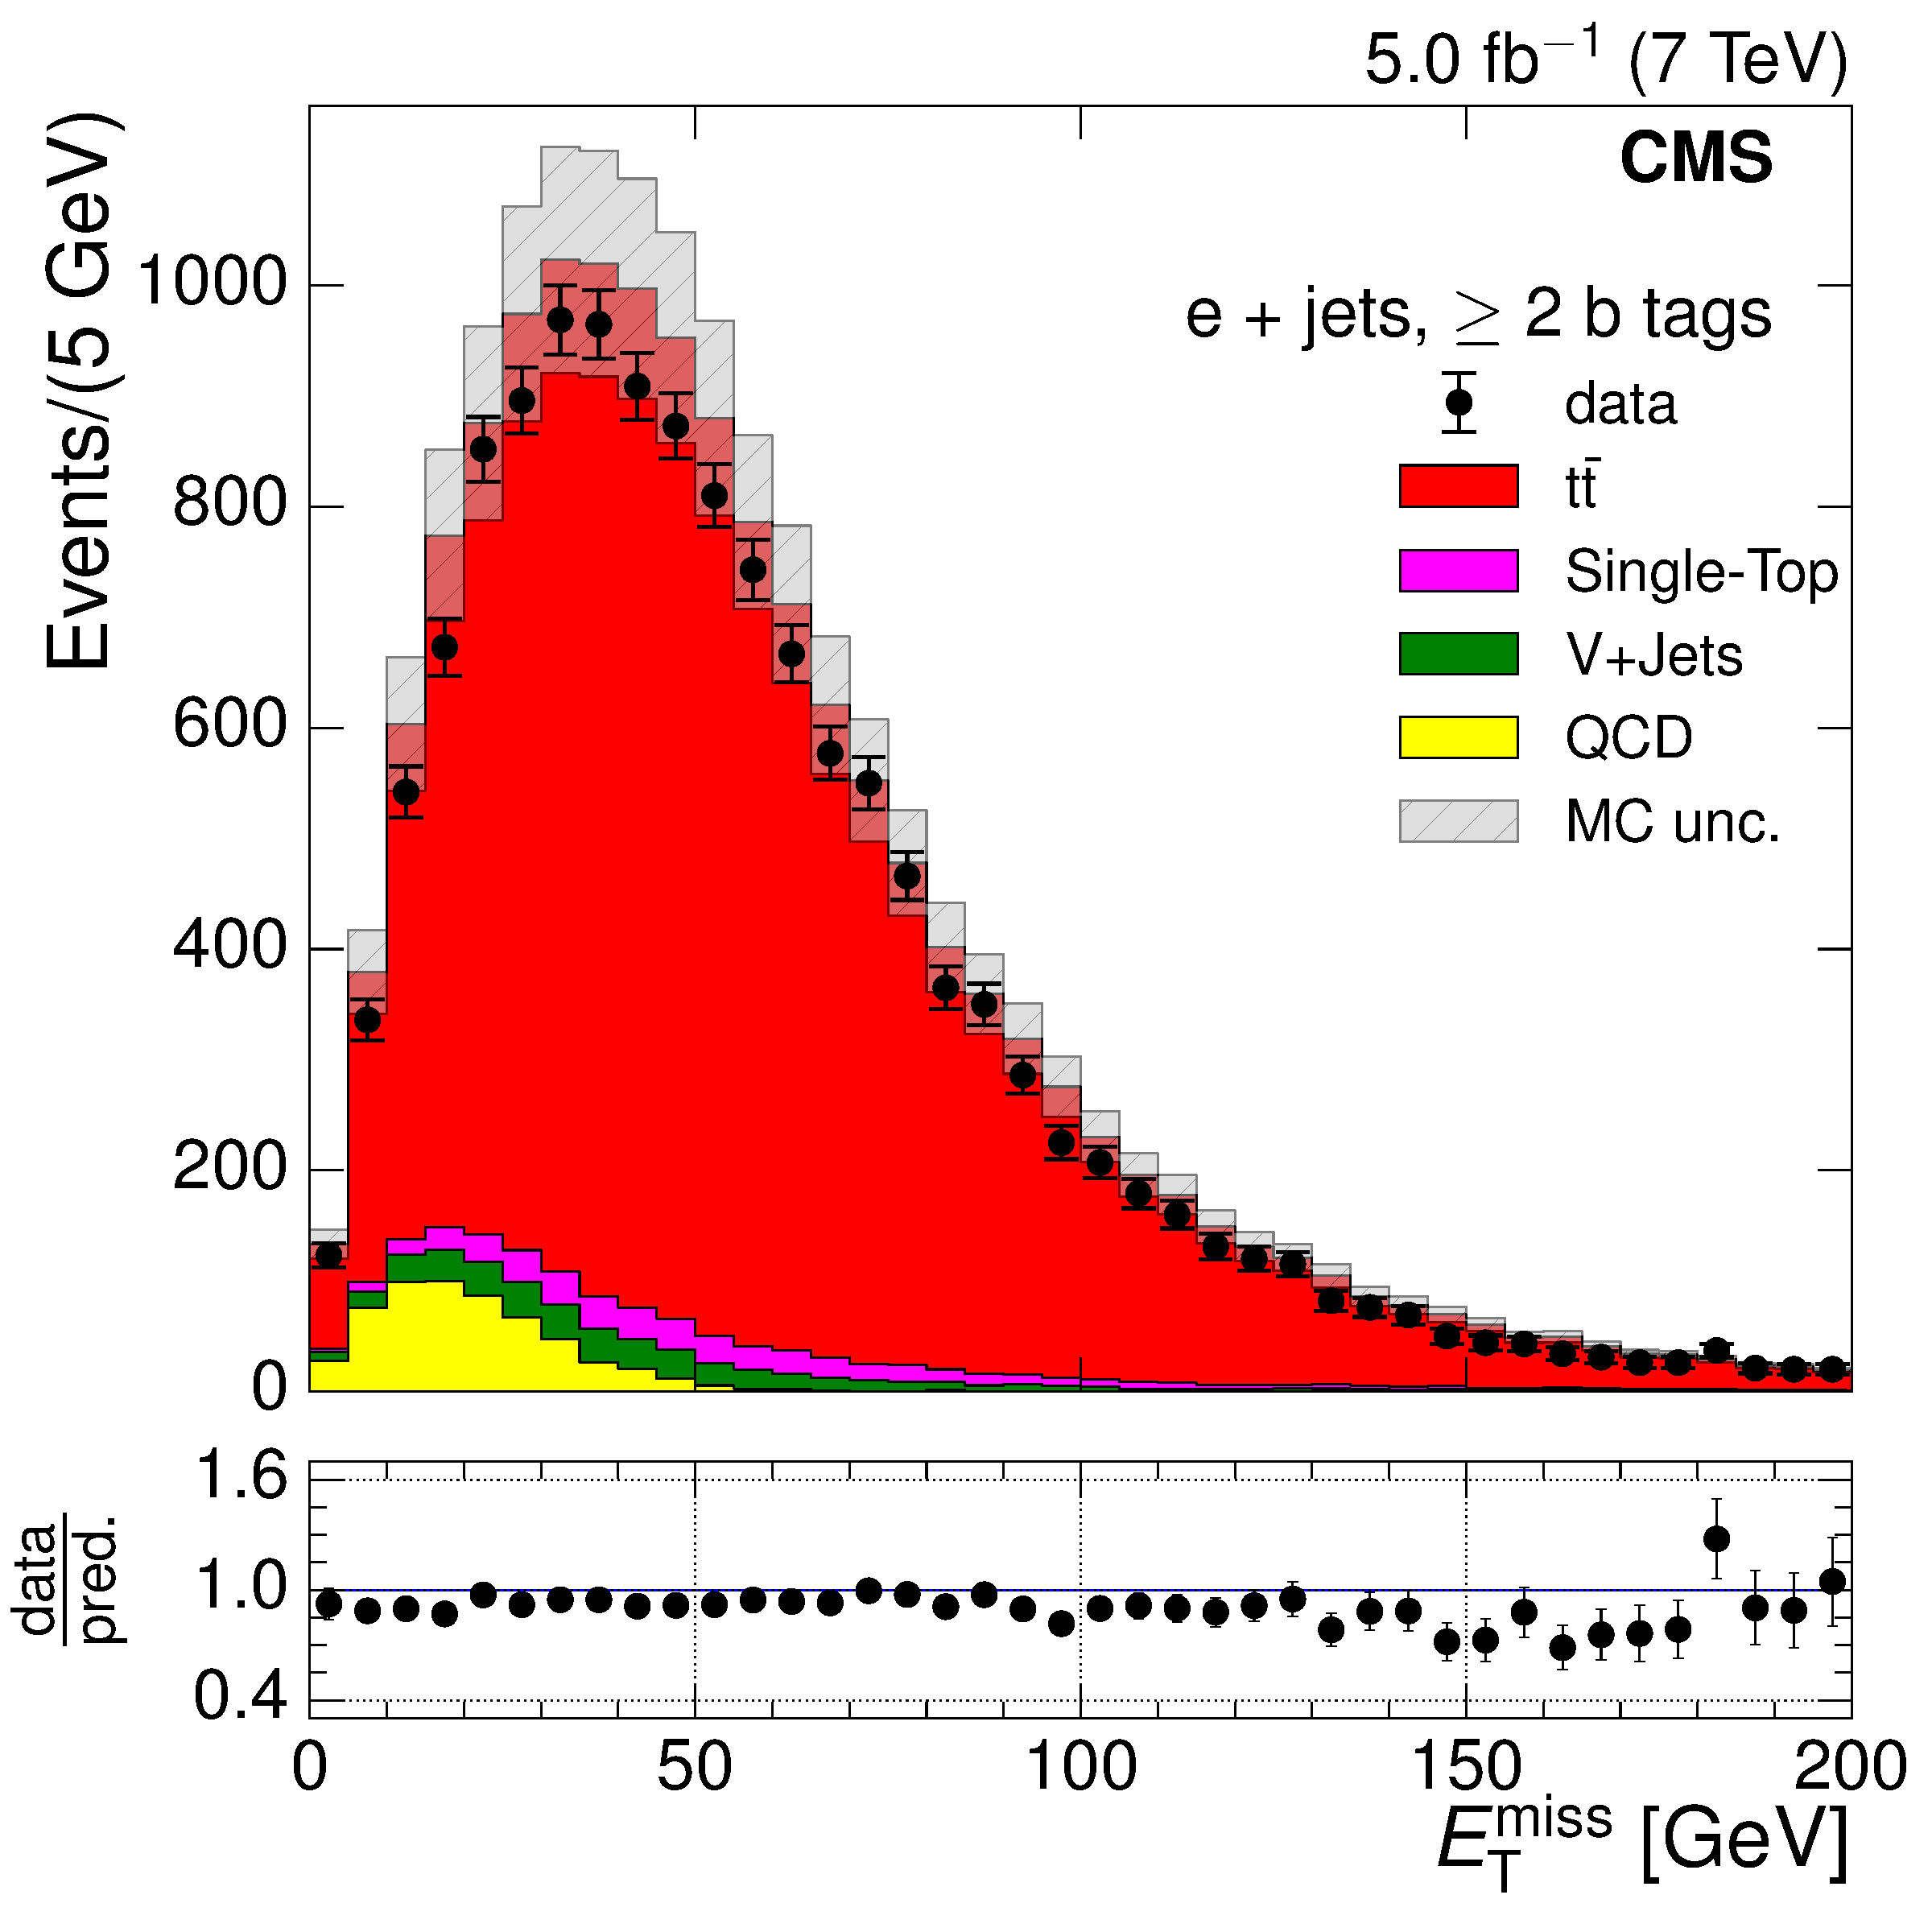
\includegraphics[width=0.45\textwidth]{Chapters/07_08_09_Analysis/Images/control_plots/before_fit/7TeV/EPlusJets_patType1CorrectedPFMet_2orMoreBtags_with_ratio}\hfill
     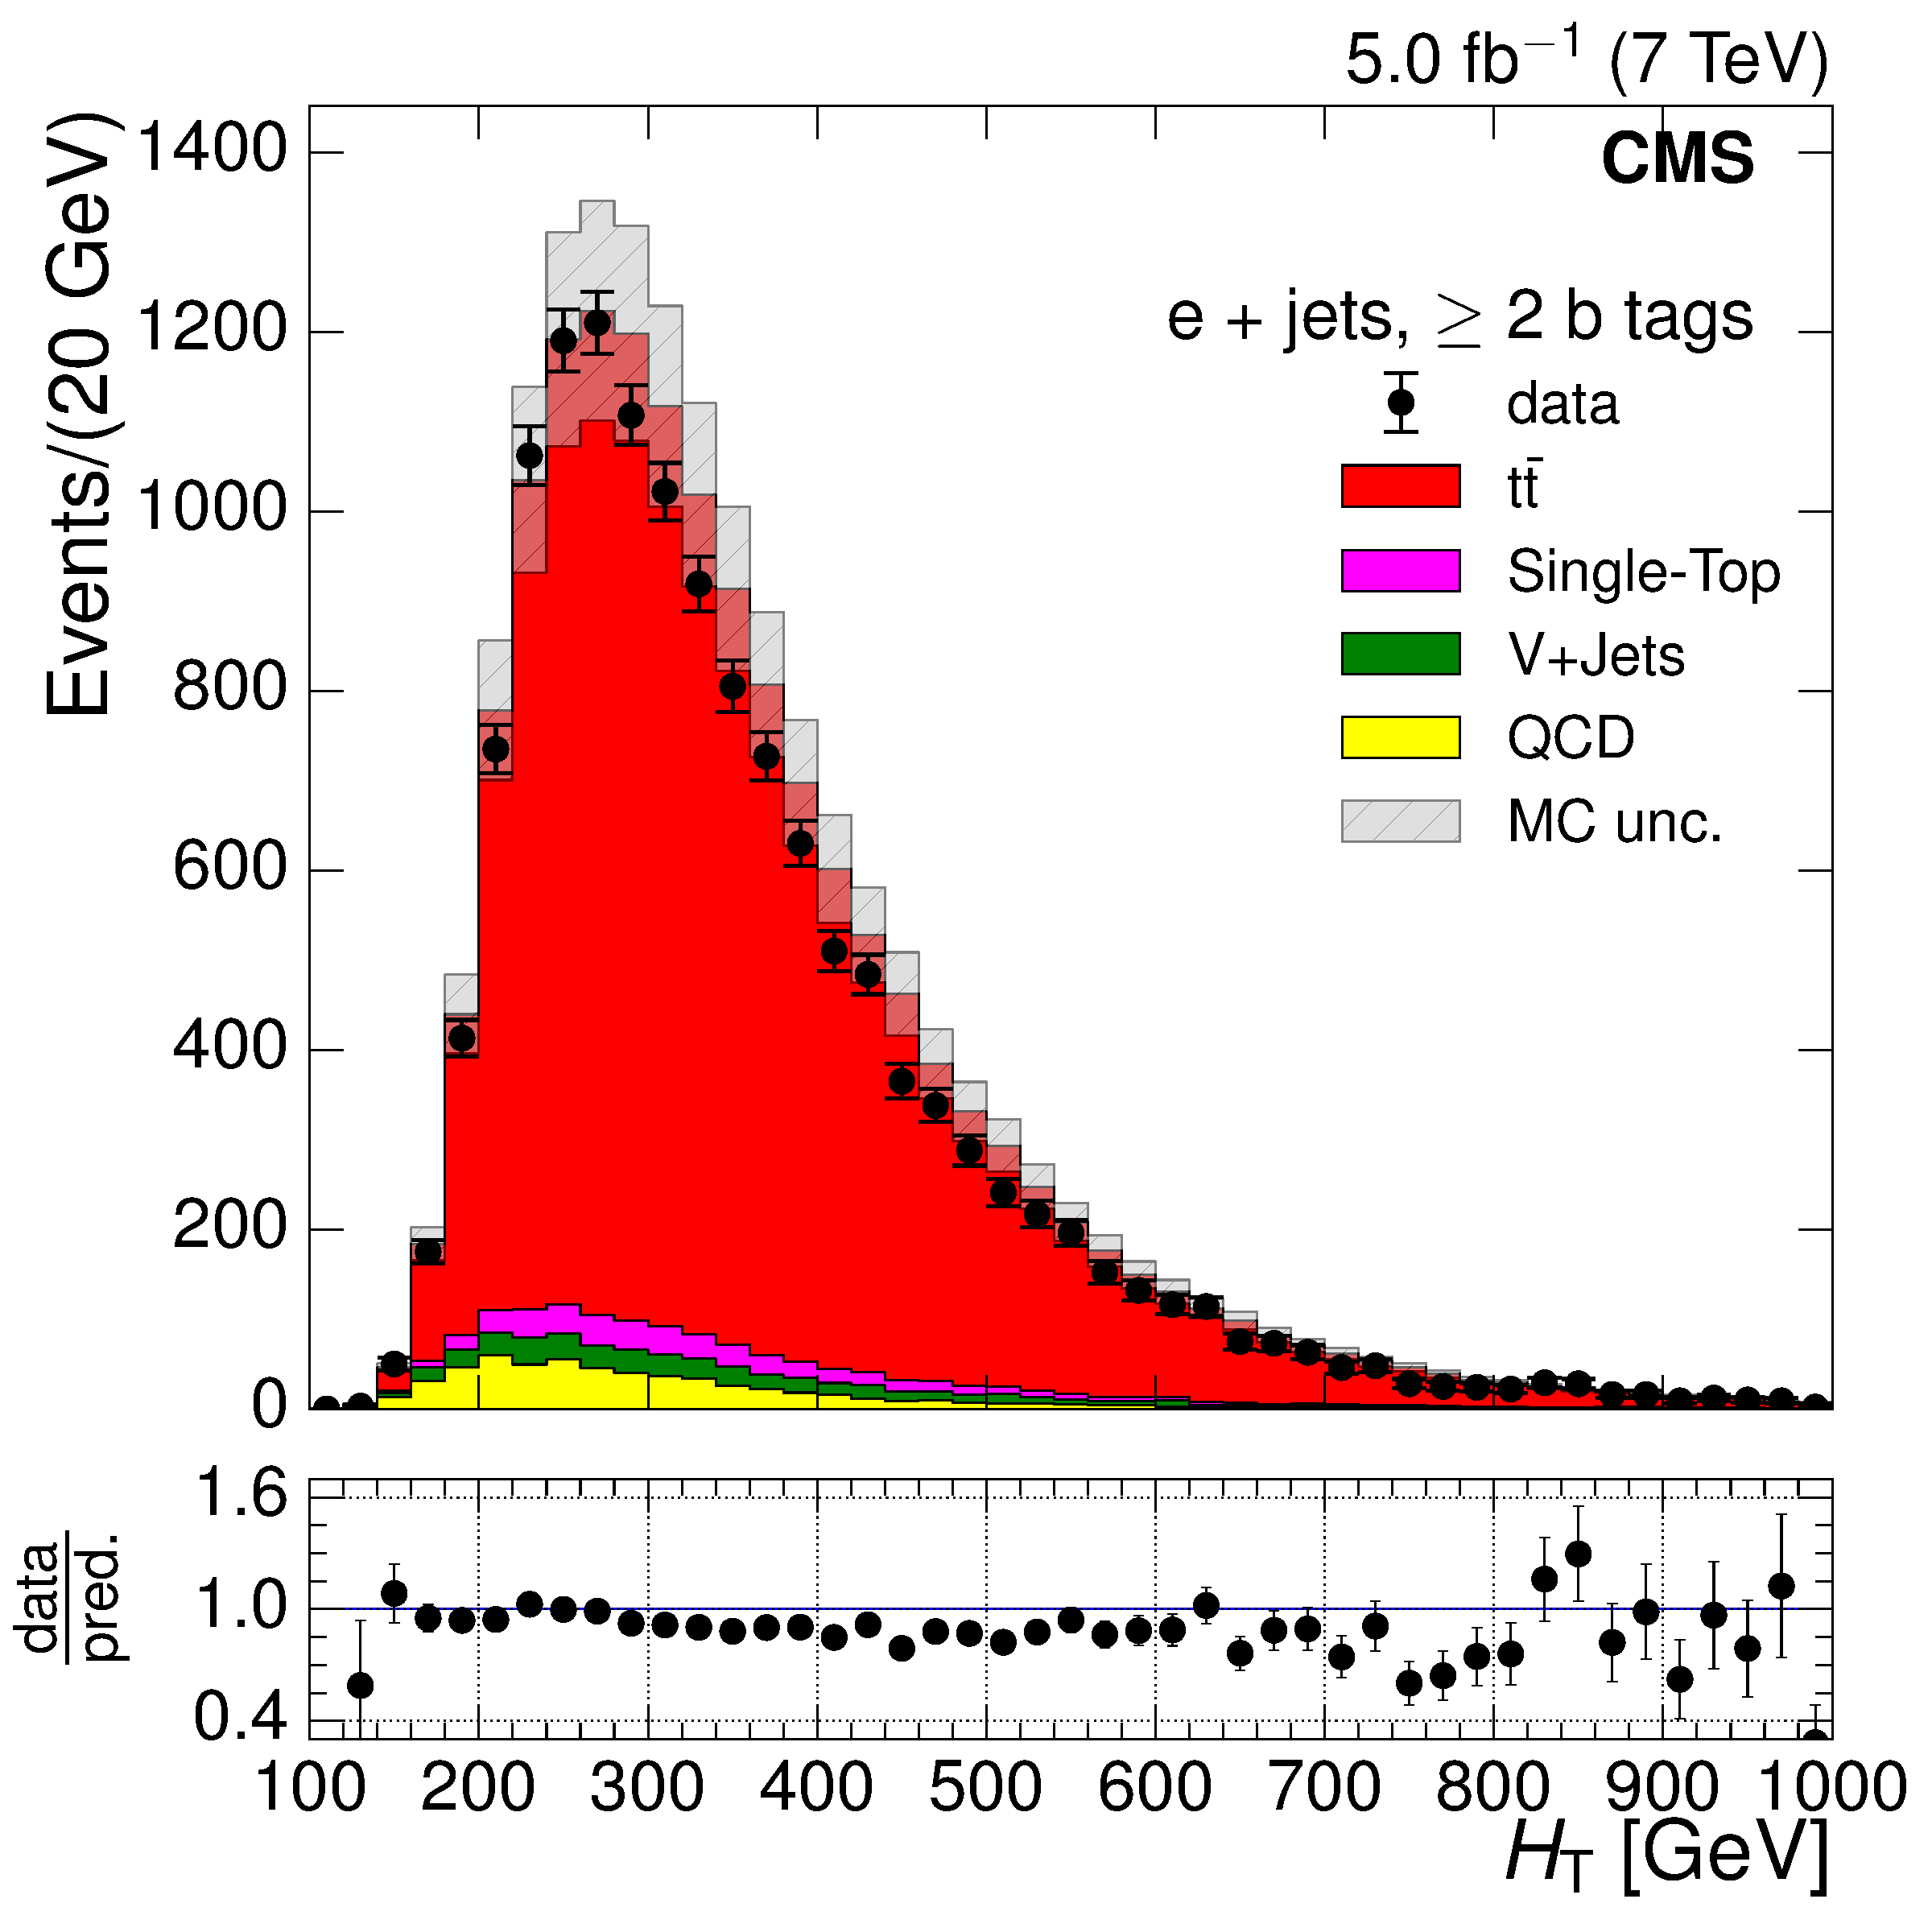
\includegraphics[width=0.45\textwidth]{Chapters/07_08_09_Analysis/Images/control_plots/before_fit/7TeV/EPlusJets_HT_2orMoreBtags_with_ratio}\\
     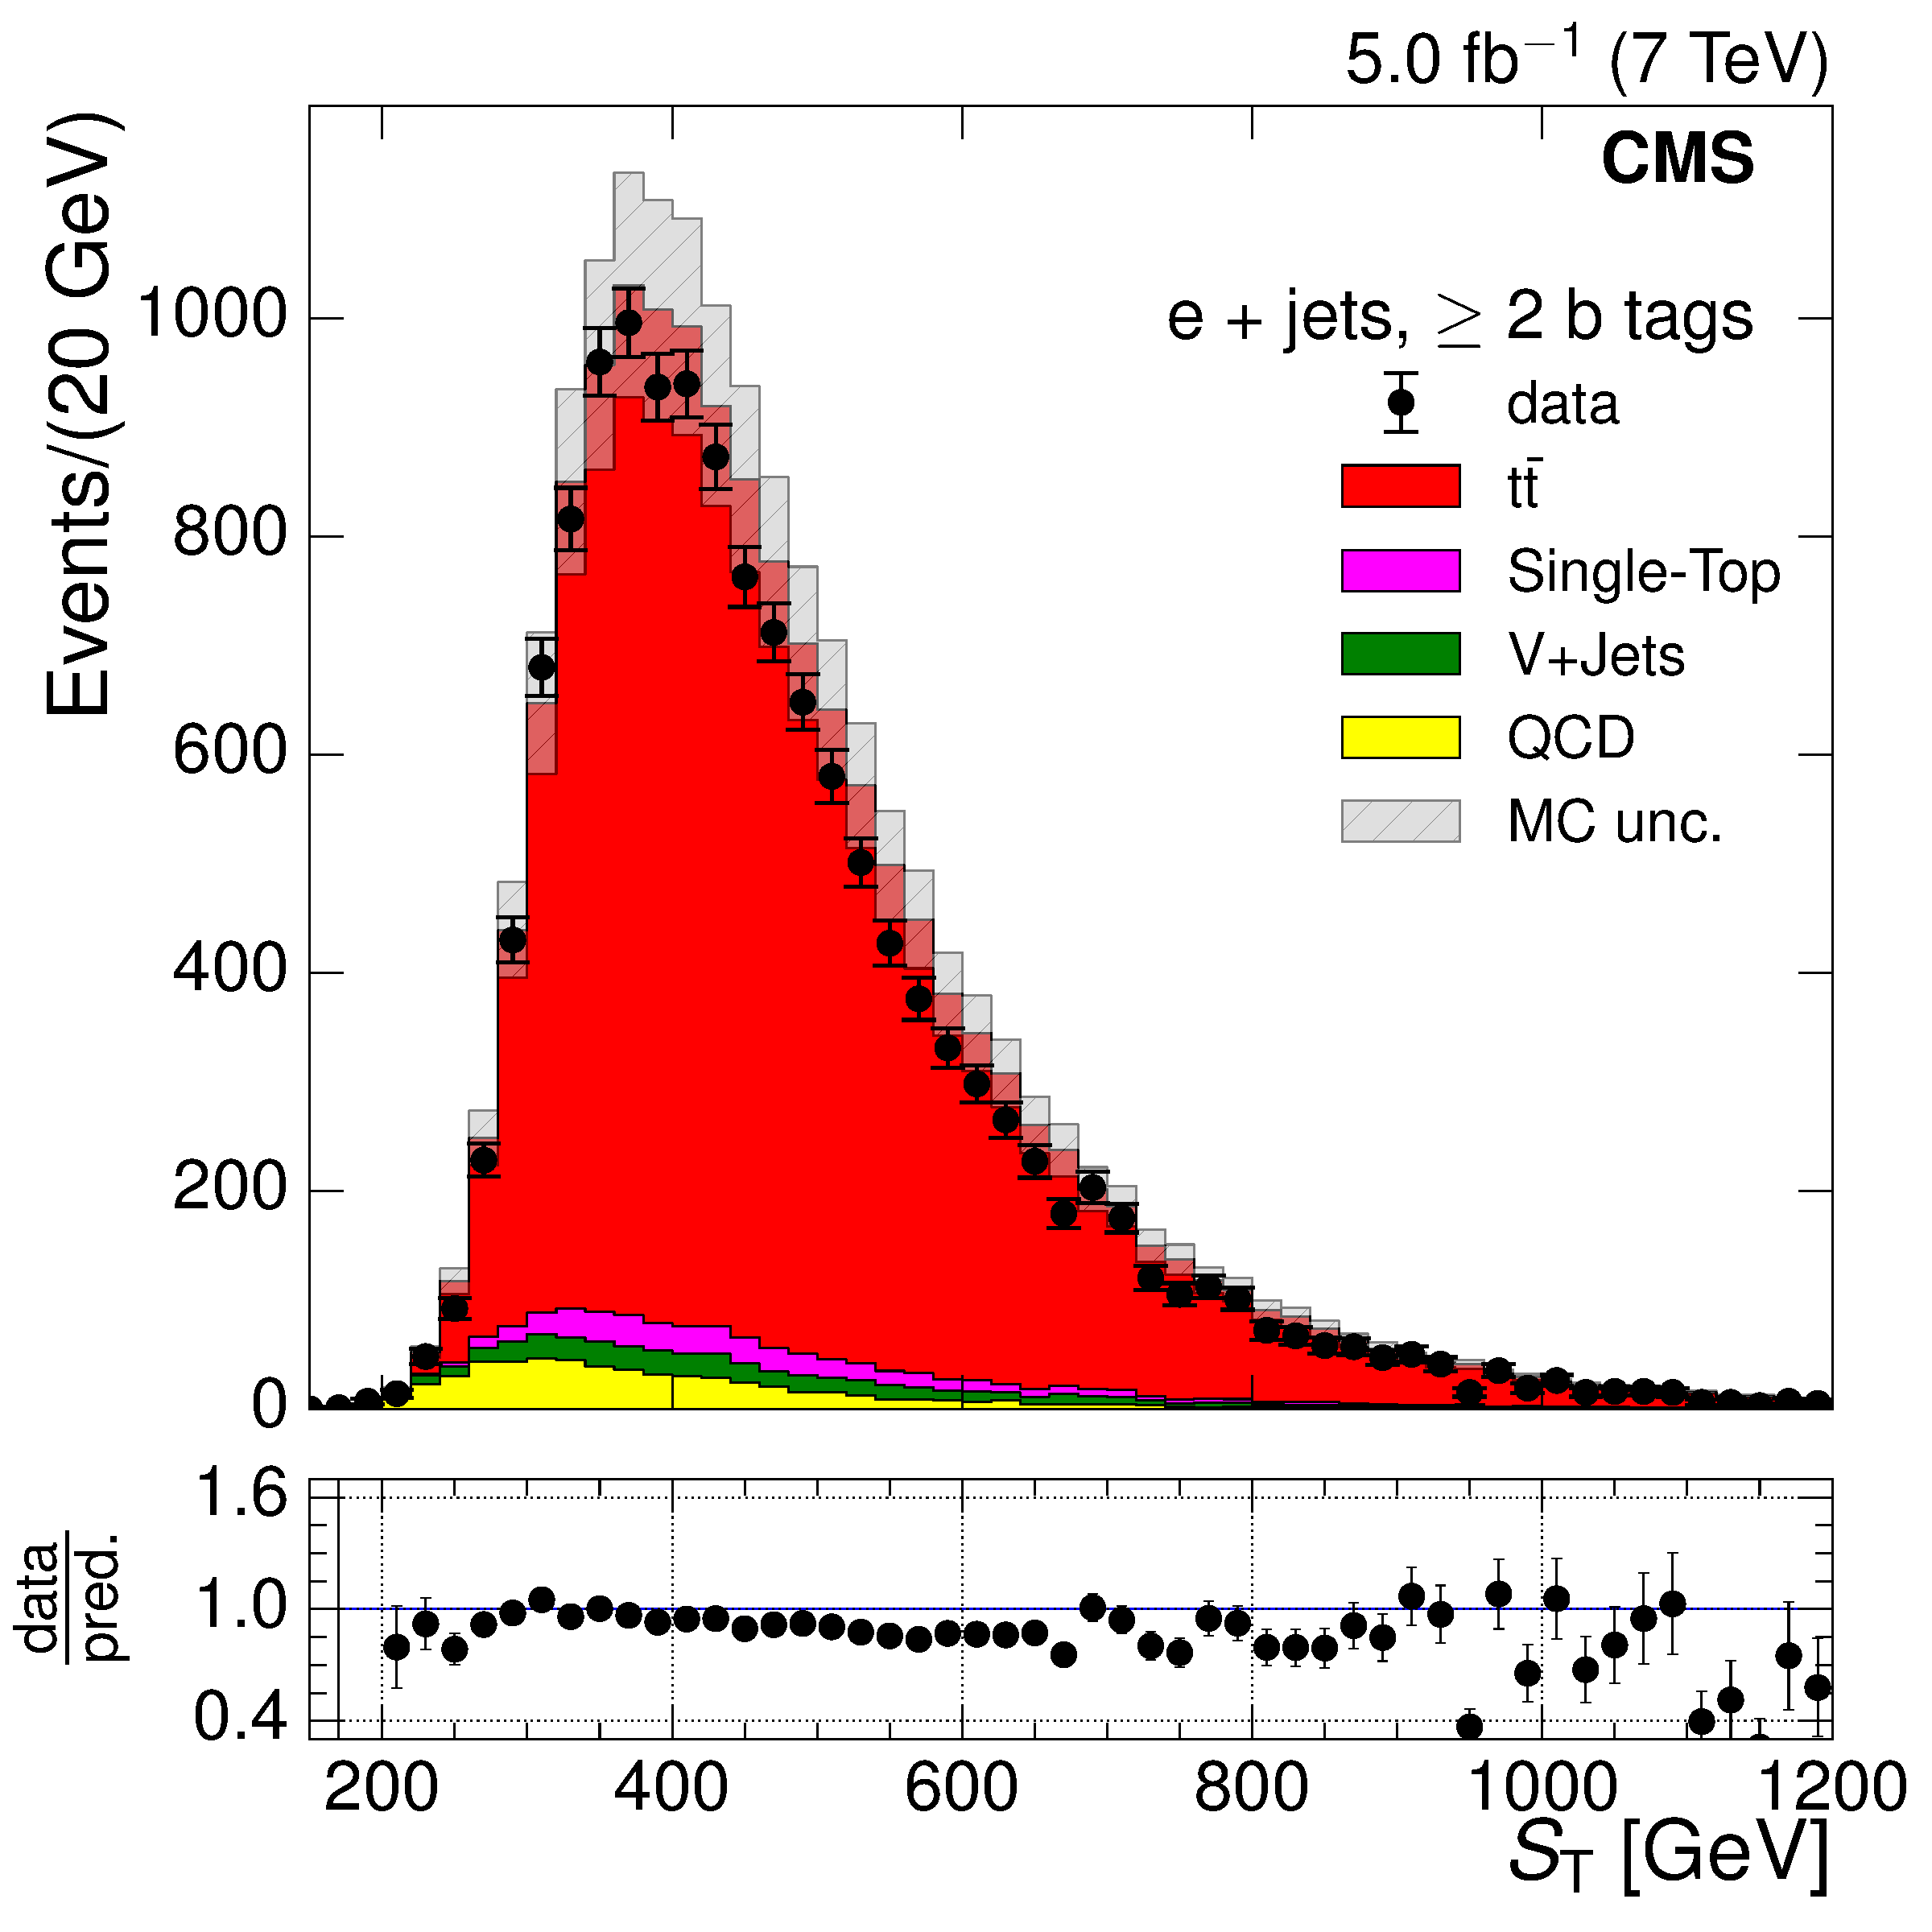
\includegraphics[width=0.45\textwidth]{Chapters/07_08_09_Analysis/Images/control_plots/before_fit/7TeV/EPlusJets_patType1CorrectedPFMet_ST_2orMoreBtags_with_ratio}\hfill
     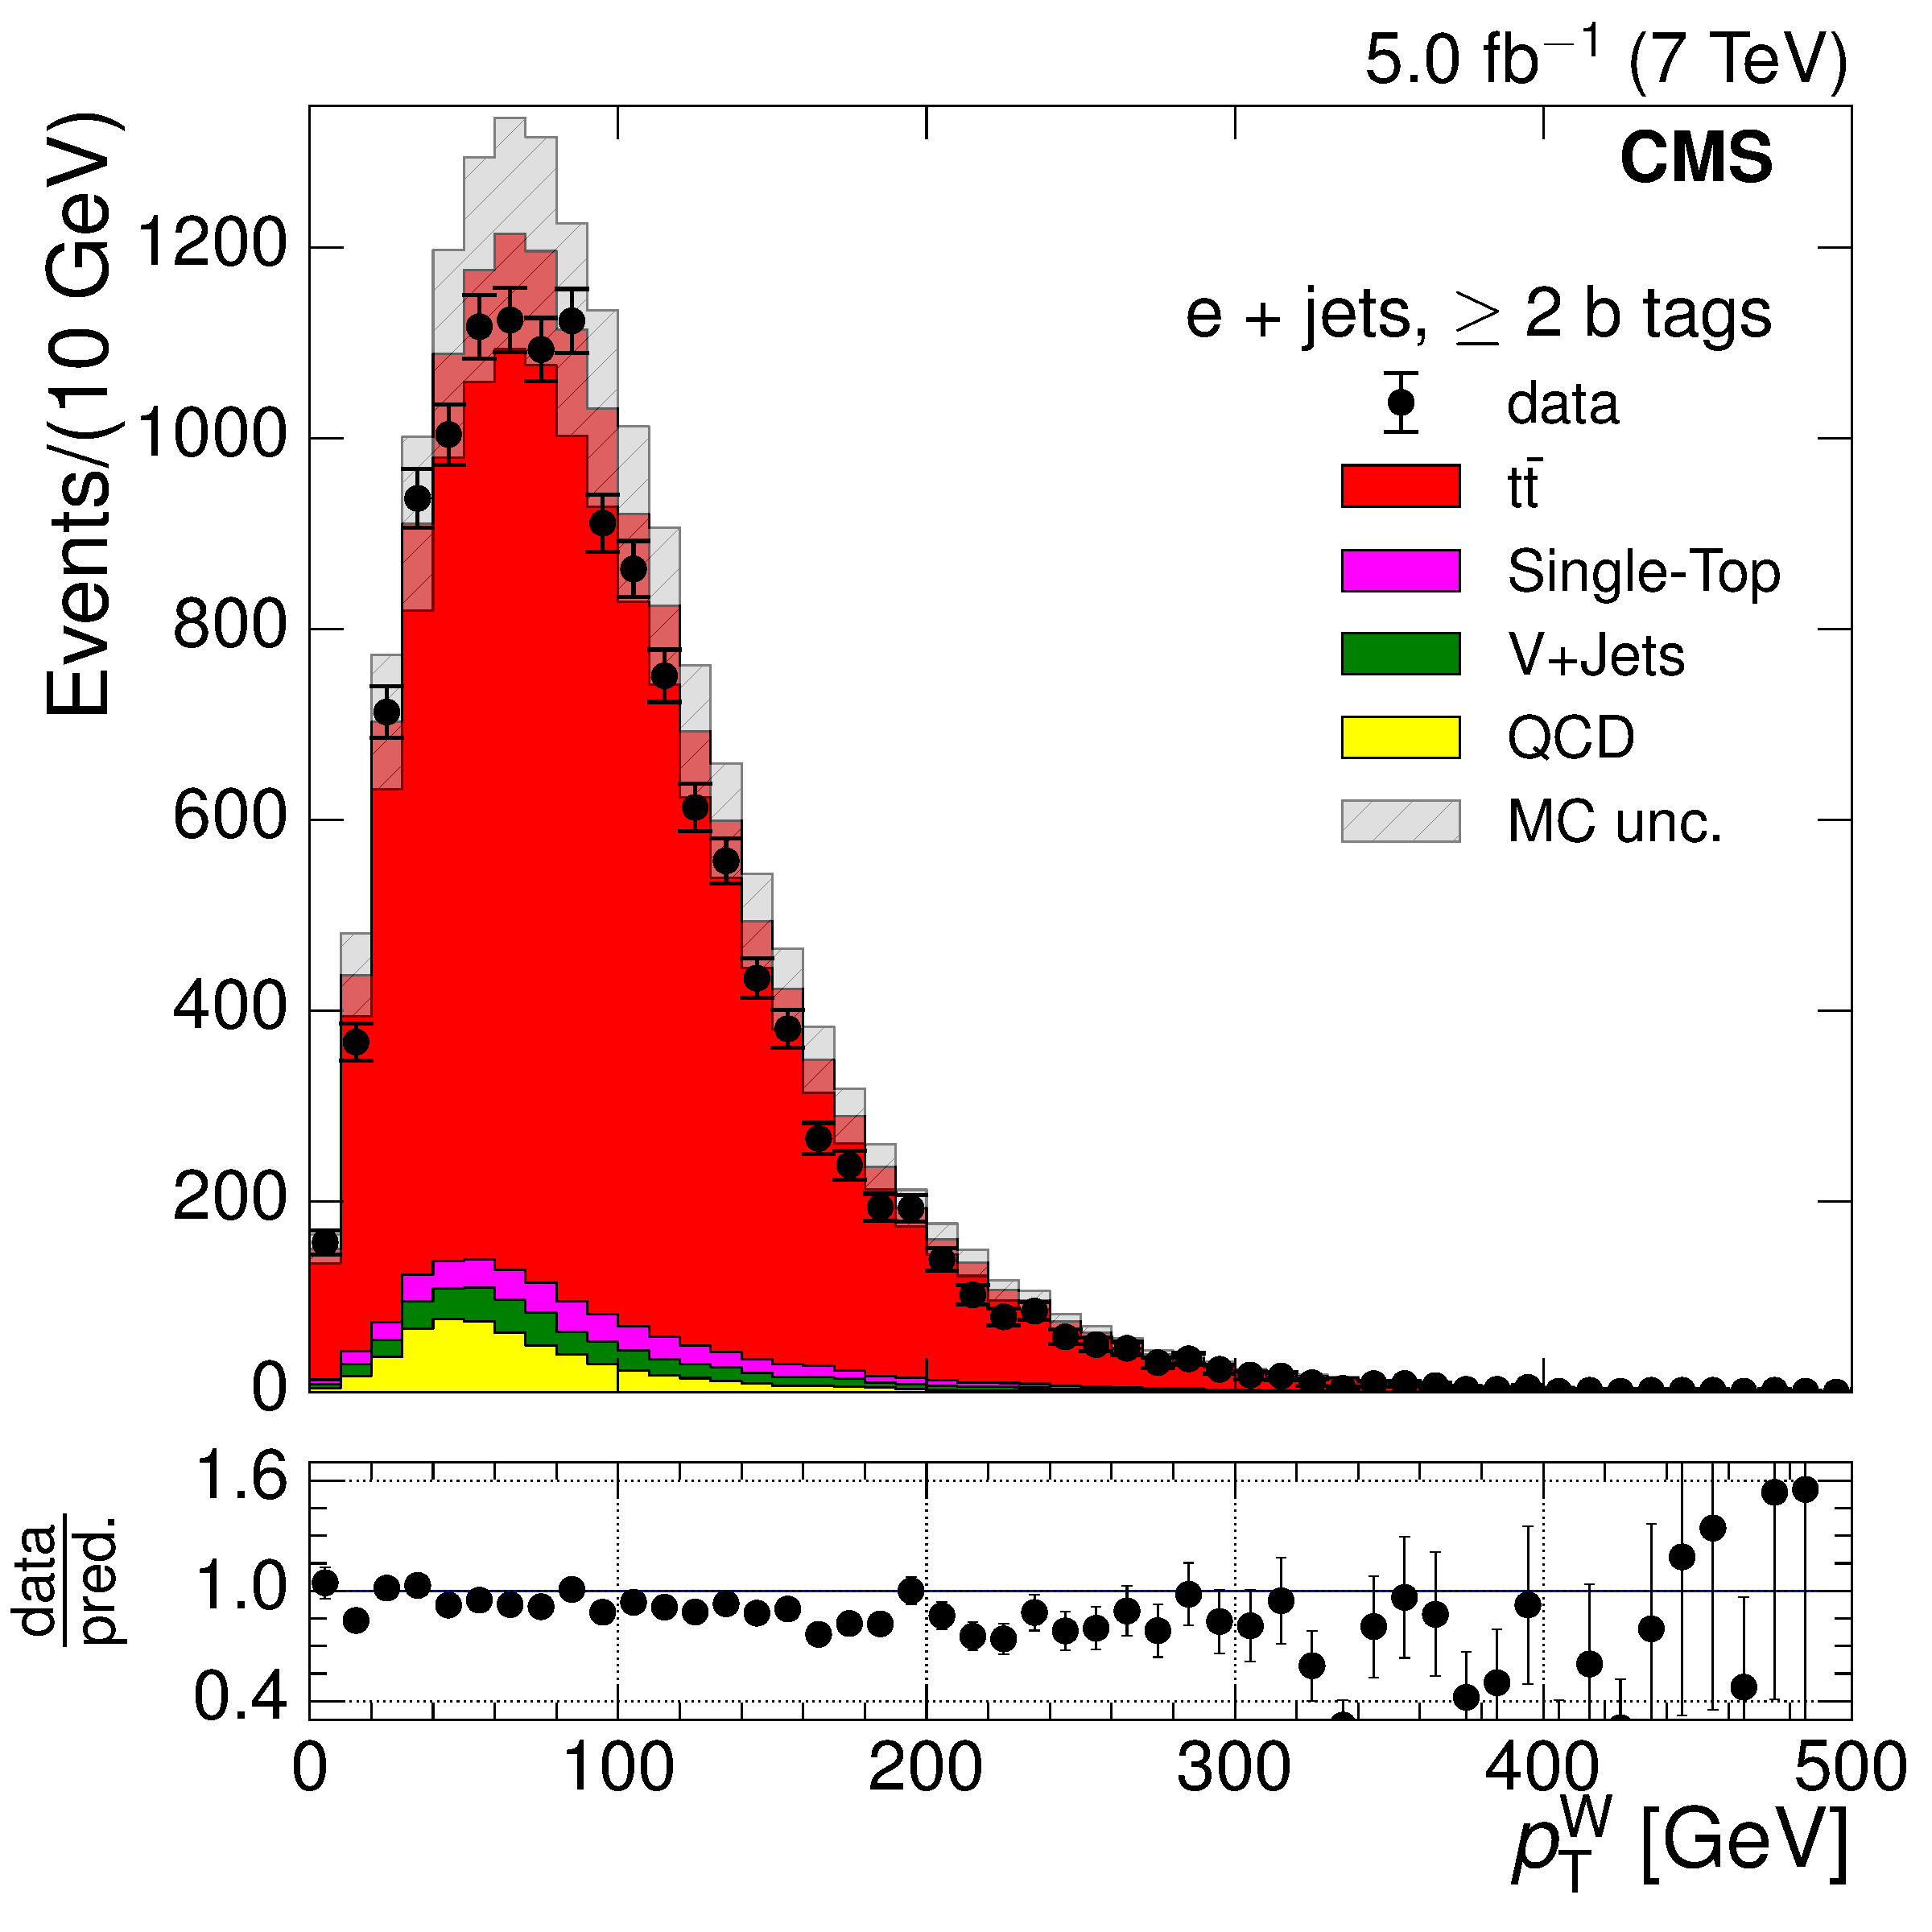
\includegraphics[width=0.45\textwidth]{Chapters/07_08_09_Analysis/Images/control_plots/before_fit/7TeV/EPlusJets_patType1CorrectedPFMet_WPT_2orMoreBtags_with_ratio}\\
     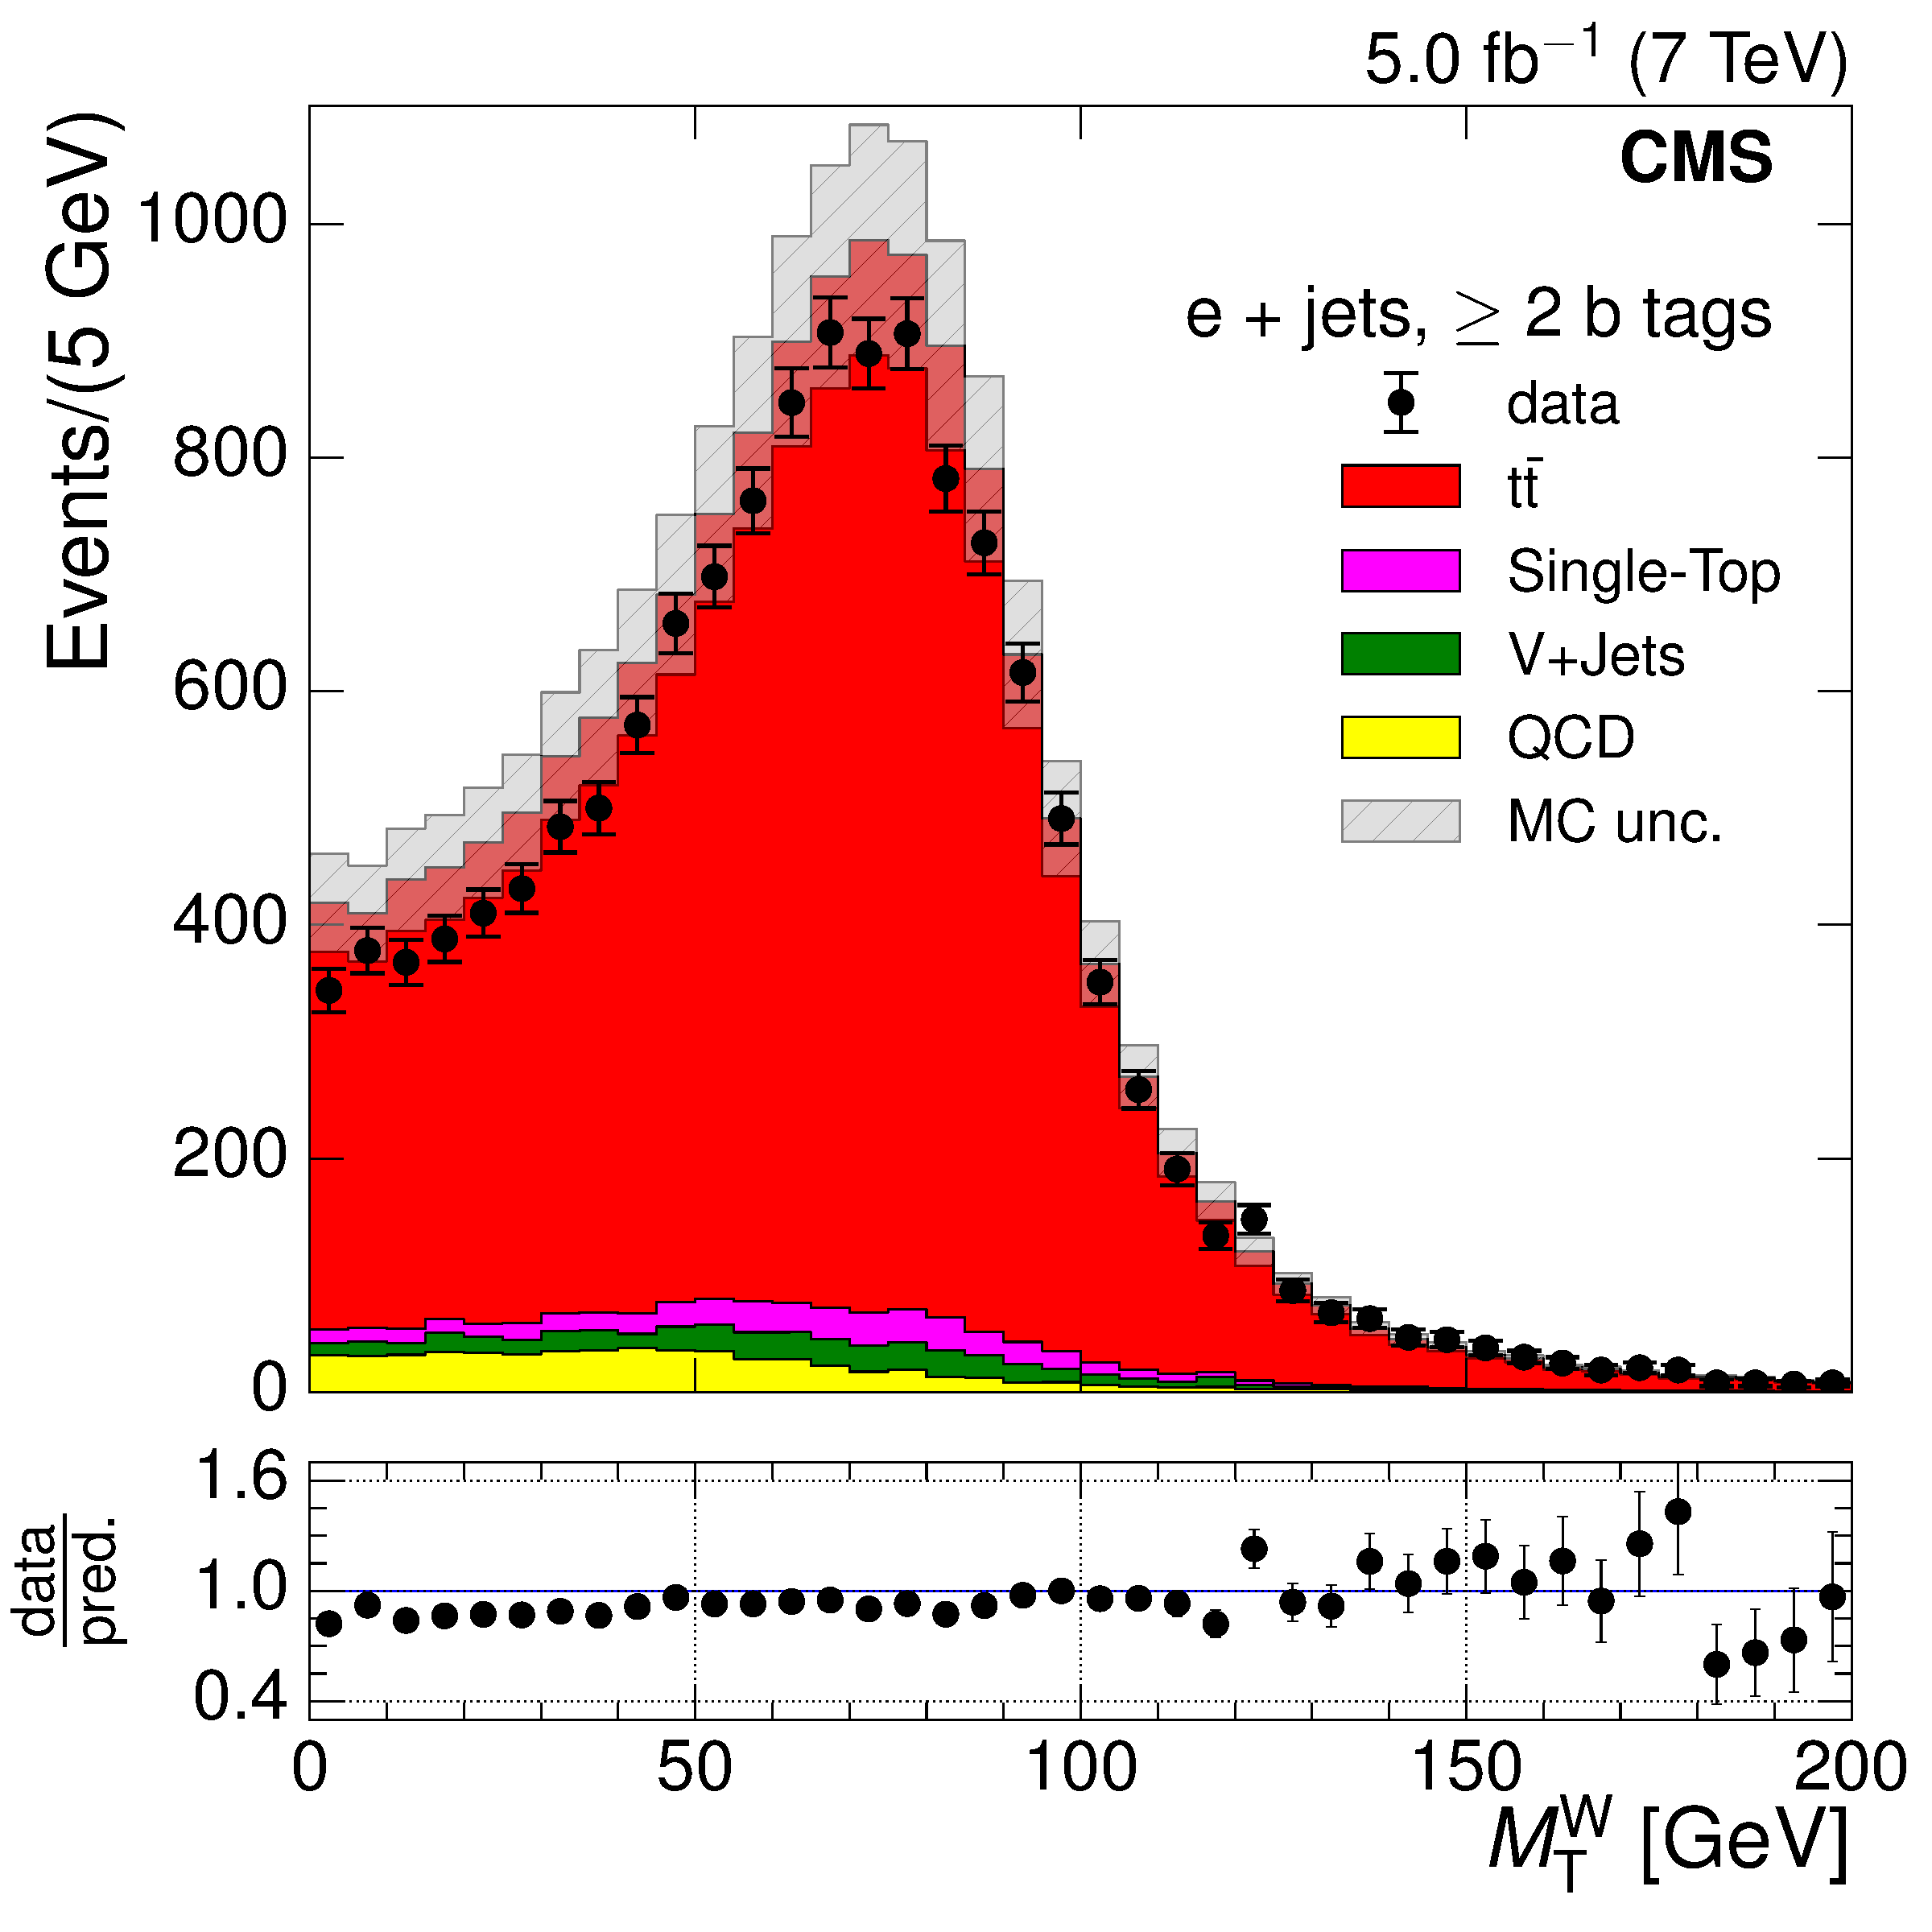
\includegraphics[width=0.45\textwidth]{Chapters/07_08_09_Analysis/Images/control_plots/before_fit/7TeV/EPlusJets_patType1CorrectedPFMet_MT_2orMoreBtags_with_ratio}\hfill
     \caption[Comparison of Monte Carlo simulation to data in the electron+jets channel after final
     selection at $\roots=7\TeV$.]{Comparison of Monte Carlo simulation to data in the electron+jets channel
     after final selection at $\roots=7\TeV$ for \met (upper left), \HT (upper right), \st (middle left), \wpt (middle
     right) and \mt (lower). The shaded region represents the \ttbar MC normalisation uncertainty. The lower
     plots show the ratio of the sum of simulated events to the data.}
     \label{fig:data_mc_comparison_7TeV_electron}
\end{figure}

\begin{figure}[hbtp]
    \centering
     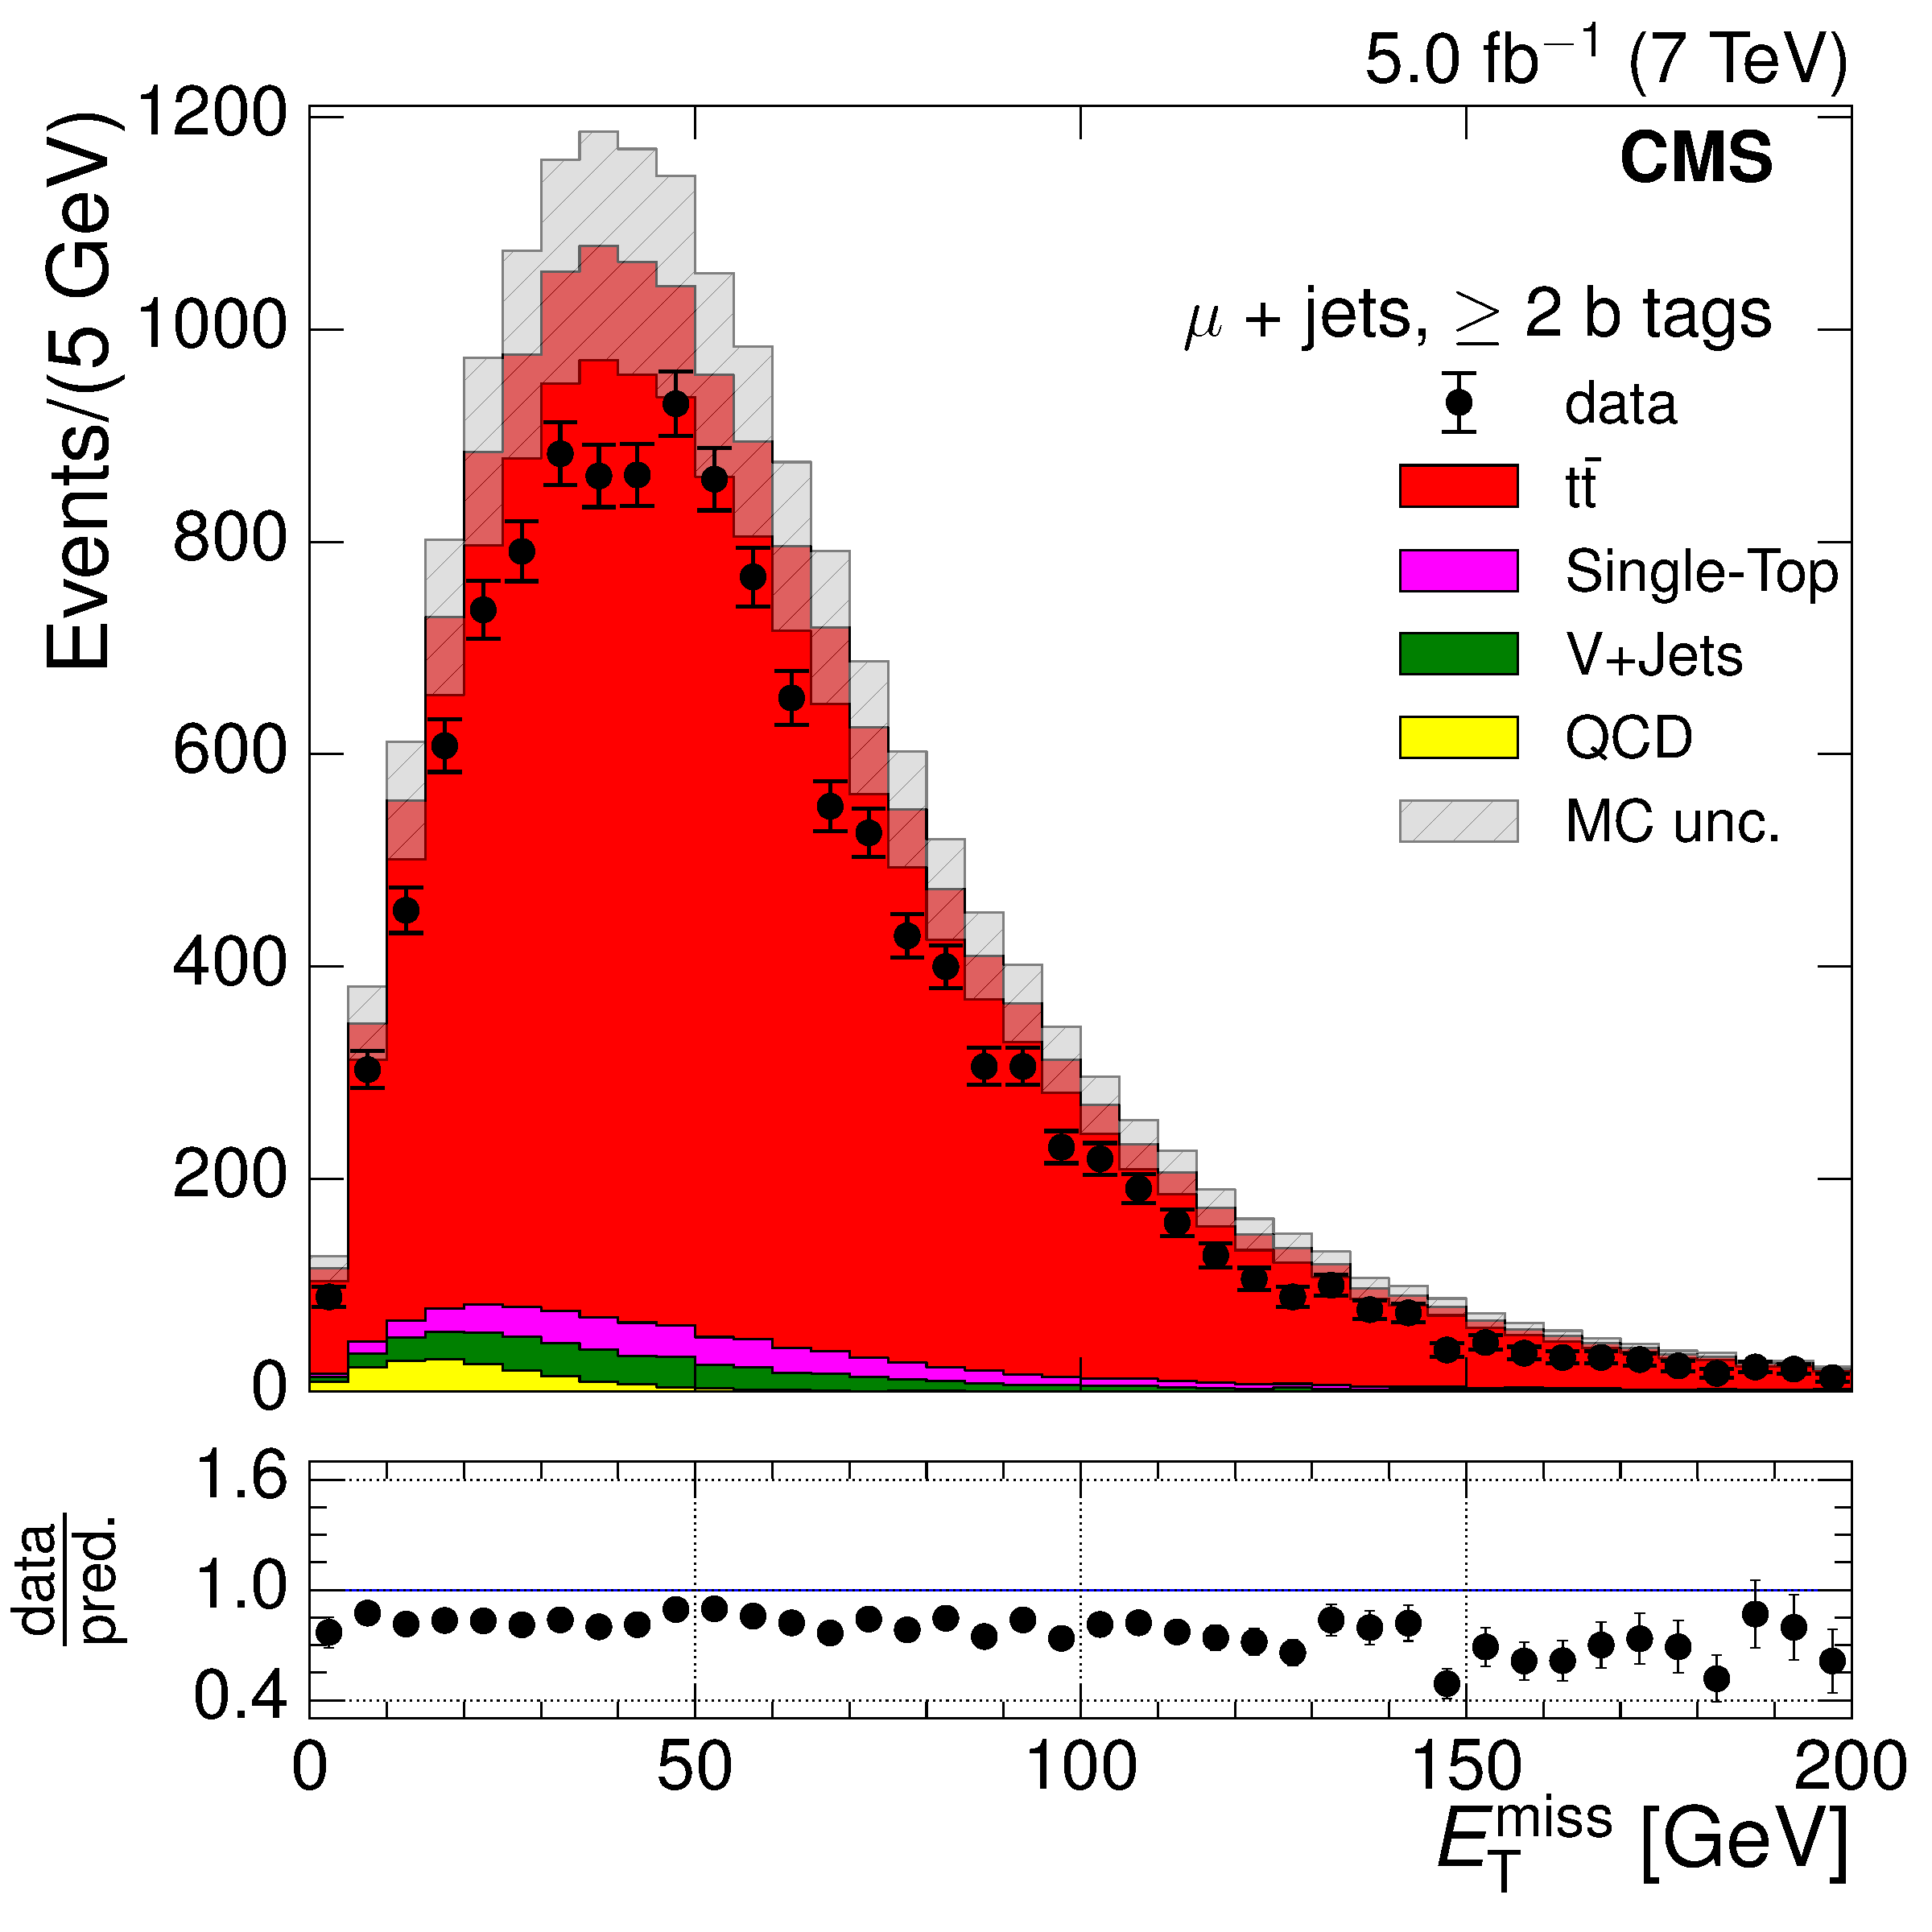
\includegraphics[width=0.45\textwidth]{Chapters/07_08_09_Analysis/Images/control_plots/before_fit/7TeV/MuPlusJets_patType1CorrectedPFMet_2orMoreBtags_with_ratio}\hfill
     \includegraphics[width=0.45\textwidth]{Chapters/07_08_09_Analysis/Images/control_plots/before_fit/7TeV/MuPlusJets_HT_2orMoreBtags_with_ratio}\\
     \includegraphics[width=0.45\textwidth]{Chapters/07_08_09_Analysis/Images/control_plots/before_fit/7TeV/MuPlusJets_patType1CorrectedPFMet_ST_2orMoreBtags_with_ratio}\hfill
     \includegraphics[width=0.45\textwidth]{Chapters/07_08_09_Analysis/Images/control_plots/before_fit/7TeV/MuPlusJets_patType1CorrectedPFMet_WPT_2orMoreBtags_with_ratio}\\
     \includegraphics[width=0.45\textwidth]{Chapters/07_08_09_Analysis/Images/control_plots/before_fit/7TeV/MuPlusJets_patType1CorrectedPFMet_MT_2orMoreBtags_with_ratio}\hfill
     \caption[Comparison of Monte Carlo simulation to data in the muon+jets channel after final
     selection at $\roots=7\TeV$.]{Comparison of Monte Carlo simulation to data in the muon+jets channel after
     final selection at $\roots=7\TeV$ for \met (upper left), \HT (upper right), \st (middle left), \wpt (middle
     right) and \mt (lower). The shaded region represents the \ttbar MC normalisation uncertainty. The lower
     plots show the ratio of the sum of simulated events to the data.}     
     \label{fig:data_mc_comparison_7TeV_muon}
\end{figure}
 
\begin{figure}[hbtp]
    \centering
     \includegraphics[width=0.45\textwidth]{Chapters/07_08_09_Analysis/Images/control_plots/before_fit/8TeV/EPlusJets_patType1CorrectedPFMet_2orMoreBtags_with_ratio}\hfill
     \includegraphics[width=0.45\textwidth]{Chapters/07_08_09_Analysis/Images/control_plots/before_fit/8TeV/EPlusJets_HT_2orMoreBtags_with_ratio}\\
     \includegraphics[width=0.45\textwidth]{Chapters/07_08_09_Analysis/Images/control_plots/before_fit/8TeV/EPlusJets_patType1CorrectedPFMet_ST_2orMoreBtags_with_ratio}\hfill
     \includegraphics[width=0.45\textwidth]{Chapters/07_08_09_Analysis/Images/control_plots/before_fit/8TeV/EPlusJets_patType1CorrectedPFMet_WPT_2orMoreBtags_with_ratio}\\
     \includegraphics[width=0.45\textwidth]{Chapters/07_08_09_Analysis/Images/control_plots/before_fit/8TeV/EPlusJets_patType1CorrectedPFMet_MT_2orMoreBtags_with_ratio}\hfill
     \caption[Comparison of Monte Carlo simulation to data in the electron+jets channel after final
     selection at $\roots=8\TeV$.]{Comparison of Monte Carlo simulation to data in the electron+jets channel
     after final selection at $\roots=8\TeV$ for \met (upper left), \HT (upper right), \st (middle left), \wpt (middle
     right) and \mt (lower). The shaded region represents the \ttbar MC normalisation uncertainty. The lower
     plots show the ratio of the sum of simulated events to the data.}
     \label{fig:data_mc_comparison_8TeV_electron}
\end{figure}
 
\begin{figure}[hbtp]
    \centering
     \includegraphics[width=0.45\textwidth]{Chapters/07_08_09_Analysis/Images/control_plots/before_fit/8TeV/MuPlusJets_patType1CorrectedPFMet_2orMoreBtags_with_ratio}\hfill
     \includegraphics[width=0.45\textwidth]{Chapters/07_08_09_Analysis/Images/control_plots/before_fit/8TeV/MuPlusJets_HT_2orMoreBtags_with_ratio}\\
     \includegraphics[width=0.45\textwidth]{Chapters/07_08_09_Analysis/Images/control_plots/before_fit/8TeV/MuPlusJets_patType1CorrectedPFMet_ST_2orMoreBtags_with_ratio}\hfill
     \includegraphics[width=0.45\textwidth]{Chapters/07_08_09_Analysis/Images/control_plots/before_fit/8TeV/MuPlusJets_patType1CorrectedPFMet_WPT_2orMoreBtags_with_ratio}\\
     \includegraphics[width=0.45\textwidth]{Chapters/07_08_09_Analysis/Images/control_plots/before_fit/8TeV/MuPlusJets_patType1CorrectedPFMet_MT_2orMoreBtags_with_ratio}\hfill
     \caption[Comparison of Monte Carlo simulation to data in the muon+jets channel after final
     selection at $\roots=8\TeV$.]{Comparison of Monte Carlo simulation to data in the muon+jets channel after
     final selection at $\roots=8\TeV$ for \met (upper left), \HT (upper right), \st (middle left), \wpt (middle
     right) and \mt (lower). The shaded region represents the \ttbar MC normalisation uncertainty. The lower
     plots show the ratio of the sum of simulated events to the data.}
     \label{fig:data_mc_comparison_8TeV_muon}
\end{figure}

\section{Binning Choice}
\label{s:binning_choice}
The differential cross sections in this analysis are measured in bins of the primary variable distributions.
The choice of bin sizes and boundaries are significant because events generated in one bin can move into
another bin after reconstruction due to the finite resolution of the detector. This altering of the number of
events, as a result of events moving into and/or out of a bin, is also important to understand so that the
final reconstructed distribution can be deconvoluted (unfolded) to the true distribution
(Section~\ref{ss:unfolding}). Migration of events between bins is taken into account in the binning choice by
evaluating two variables defined as purity ($p^k$) and stability ($s^k$), which are functions of how well a
variable is reconstructed:
\begin{align}
\label{eq:purity_and_stability}
p^k = \frac{N_{\rec\&\gen}^k}{N_{\rec}^k}\\
s^k = \frac{N_{\rec\&\gen}^k}{N_{\gen}^k}.
\end{align}
$N_{\rec\&\gen}^k$ is the number of events generated and reconstructed in bin $k$,
$N_{\rec}^k$ is the number of events reconstructed in bin $k$ and $N_{\gen}^k$ is the number of events
generated in bin $k$. The stability of a bin is sensitive to the migration of events out of a bin, while the
purity is sensitive to the migration of events into a bin (see Figure~\ref{fig:purity_and_stability}).

\begin{figure}[hbtp]
	\centering
     \includegraphics[width=0.8\textwidth]{Chapters/07_08_09_Analysis/Images/purity_and_stability}
     \caption[Graphical representation of bin purity and stability.]{Stability quantifies the migration of
     events out of a bin while purity quantifies the migration of events into a bin. Both quantities compare
     the bin in which an event is generated to the range in which they are reconstructed.}
     \label{fig:purity_and_stability}
 \end{figure}

A high number of bins allows for a fine granularity in the measurement, but bins must also be selected such
that good statistics are maintained in all bins, thereby avoiding the large relative statistical error that
would result from small bins with few events.

In light of the requirements of minimising event migration between bins and maintaining sufficient numbers of
events, the bin boundaries for each primary variable distribution were chosen such that all bins have
\begin{itemize}
  \item purity and stability values of 0.5 or greater
  \item at least 100 events 
\end{itemize}
This means that at least half of the events generated in a bin remain in that bin after reconstruction, and
that at least half of the events reconstructed in a bin were generated in that bin. Although, ideally, higher
values of purity and stability would have been preferable to further minimise bin-to-bin migration, and
thereby reduce the unfolding uncertainty and the amount of regularisation needed in the unfolding procedure
(Section~\ref{ss:unfolding}), a compromise between minimising migration and adequate statistics was required.

The determination of the bin boundaries following these criteria is carried out simultaneously in (and
therefore the binning is identical in) both centre of mass energies and both the electron+jets and muon+jets
channel. Plots of generated versus reconstructed events in simulation for all primary variables are shown in
the electron+jets channel in Figure~\ref{fig:binning_7TeV_electron} for $\roots=7\TeV$ and in
Figure~\ref{fig:binning_8TeV_electron} for $\roots=8\TeV$. The corresponding plots in the muon+jets channel
are shown in Figures~\ref{fig:binning_7TeV_muon} and \ref{fig:binning_8TeV_muon} in
Appendix~\ref{as:binning_muon}.

\begin{figure}[hbtp]
	\centering
     \includegraphics[width=0.48\textwidth]{Chapters/07_08_09_Analysis/Images/binning/electron_MET_7TeV}\hfill
     \includegraphics[width=0.48\textwidth]{Chapters/07_08_09_Analysis/Images/binning/electron_HT_7TeV}\\
     \includegraphics[width=0.48\textwidth]{Chapters/07_08_09_Analysis/Images/binning/electron_ST_7TeV}\hfill
     \includegraphics[width=0.48\textwidth]{Chapters/07_08_09_Analysis/Images/binning/electron_MT_7TeV}\\
	 \includegraphics[width=0.48\textwidth]{Chapters/07_08_09_Analysis/Images/binning/electron_WPT_7TeV}\hfill
	 \caption[Generated versus reconstructed distributions of the primary variable at $\roots=7\TeV$.]{Generated
	 versus reconstructed distributions of the primary variables \met (upper left), \HT (upper right), \st (middle
	 left), \mt (middle right) and \wpt (lower) with horizontal and vertical lines representing the boundaries of
	 the selected bins at $\roots=7\TeV$ in the electron+ jets channel. These distributions are obtained using
	 \ttbar simulation.}
     \label{fig:binning_7TeV_electron}
\end{figure}

\begin{figure}[hbtp]
    \centering
     \includegraphics[width=0.48\textwidth]{Chapters/07_08_09_Analysis/Images/binning/electron_MET_8TeV}\hfill
     \includegraphics[width=0.48\textwidth]{Chapters/07_08_09_Analysis/Images/binning/electron_HT_8TeV}\\
     \includegraphics[width=0.48\textwidth]{Chapters/07_08_09_Analysis/Images/binning/electron_ST_8TeV}\hfill
     \includegraphics[width=0.48\textwidth]{Chapters/07_08_09_Analysis/Images/binning/electron_MT_8TeV}\\
	 \includegraphics[width=0.48\textwidth]{Chapters/07_08_09_Analysis/Images/binning/electron_WPT_8TeV}\hfill
	 \caption[Generated versus reconstructed distributions of the primary variables at $\roots=8\TeV$.]{Generated
	 versus reconstructed distributions of the primary variables \met (upper left), \HT (upper right), \st
	 (middle left), \mt (middle right) and \wpt (lower) with horizontal and vertical lines representing the
	 boundaries of the selected bins at $\roots=8\TeV$ in the electron+ jets channel. These distributions are
	 obtained using \ttbar simulation.}
     \label{fig:binning_8TeV_electron}
 \end{figure}
\FloatBarrier

\section{Maximum Likelihood Fit}
\label{s:maximum_likelihood_fit}
A maximum log likelihood fit of four process shapes, or templates, to data in each bin of the primary
variables is used to obtain the number of events from each process in each bin. The four templates used
are:
\begin{itemize}
  \item {\ttbar}
  \item{single-top}
  \item{V+jets (W+jets + Z+jets)}
  \item{QCD multi-jet} 
\end{itemize}

The fit is carried out in three fitting variables, because no individual variable is able to distinguish
between all four templates in the fit. The following three fitting variables are used:
\begin{itemize}
  \item {the absolute pseudorapidity of the lepton (\abseta)}
  \item {the three-dimensional angle between the lepton and the nearest \bjet ($\alpha$)}
  \item {invariant mass of the three jets with the highest \pt sum (\Mthree)}
\end{itemize}

The fit is carried out by maximising the log of the likelihood function (LL):
\begin{equation}
\label{log_likelihood}
LL\left(x_i, d_i\right) = -2 \log{\prod\limits_{i}\frac{x_i^{d_i}\cdot
e^{-x_i}}{d_i!}}=-2\sum\limits_{i}\log{\left(\frac{x_i^{d_i}\cdot e^{-x_i}}{d_i!}\right)}.
\end{equation}

where $i$ is the bin index in the template, $x_i$ is the total of all the templates in bin $i$, and $d_i$ is
the observed number of data events in  bin $i$. $x_i$ is defined to be
\begin{equation}
\label{eq:sum_mc}
x_i = \sum\limits_{j}N_{j}x_{i\,j},\;\text{with}\;\sum\limits_{i}x_{i\,j}=1\ \text{for each process}.
\end{equation}

where $x_{i\,j}$ represents the templates and $N_{j}$ represents the normalisations of the templates \ie the
fit parameters. Fitting using more than one variable (the three aforementioned fitting variables), the
log likelihoods are summed:
\begin{equation}
\label{eq:log_L_final}
LL\left(x, d\right) = -\frac{2}{n} \sum\limits_{k=1,n} \log{L_k}
\end{equation}

where $L_k$ is the likelihood function of each of the different fit variables. Here the division by $n$
accounts for the fact that the same information is used in all three fit variables, and so full correlation is
assumed between the three fitting variables, which provides a conservative estimate of the uncertainties in
the resulting fitted parameters. The fit operates by adjusting the normalisation of each template with the aim
of equating $x_{i}$ and $d_{i}$ in each bin of each template. The starting normalisations in the templates are
obtained from simulation after the full selection has been applied (this includes the QCD template, although
the shape for this is obtained from data).

\subsection{Choice of templates}
\label{choice_of_templates}

\ttbar, single-top and V+jets templates are taken from simulation, while the QCD template is extracted from
data as described in Section~\ref{ss:background_selection}. The W+jets and Z+jets templates are combined
firstly due to the similar shapes of the distributions in these two background processes, and secondly due to
limited statistics available in simulation. The four template shapes in each of the three fitting variables at
$\roots=7\TeV$ in both channels are shown in Figure~\ref{fig:fit_variable_distributions_7TeV}. The
corresponding plots for $\roots=8\TeV$ are shown in Appendix~\ref{as:fitting_variables_distributions}.

This combination of fitting variables was selected because they are only weakly correlated to the primary
variables under investigation, and they show good discrimination between the four templates.
Single top events have similar signatures to \ttbar events, with a central lepton from the decay of the single
top, leading to a single top template that is similar to the \ttbar template in the electron \abseta and muon
\abseta distributions. In the $\alpha$ distribution, the similarity is attributable to the fact that the
closest \bjet from the lepton is generally a \bjet from the decay of a \tquark. However, the average boost for
single top events is lower than in \ttbar events, leading to a wider single top template.
The \Mthree variable will be a combination of the jets from the hadronically decaying \tquark (a \bjet and two
other jets from the \W-boson, which may include a second \bjet) in \ttbar events, whereas in the other
templates, \Mthree will simply correspond to some random combination of jets in the event. Hence, \Mthree shows the
best discrimination between the single top and \ttbar templates.

\begin{figure}[hbtp]
    \centering
     \includegraphics[width=0.45\textwidth]{Chapters/07_08_09_Analysis/Images/7TeV/fit_variables/electron/MET/electron_absolute_eta/MET_inclusive_electron_absolute_eta_2orMoreBtags_templates}\hfill
     \includegraphics[width=0.45\textwidth]{Chapters/07_08_09_Analysis/Images/7TeV/fit_variables/muon/MET/muon_absolute_eta/MET_inclusive_muon_absolute_eta_2orMoreBtags_templates}\\
     \includegraphics[width=0.45\textwidth]{Chapters/07_08_09_Analysis/Images/7TeV/fit_variables/electron/MET/angle_bl/MET_inclusive_angle_bl_2orMoreBtags_templates}\hfill
     \includegraphics[width=0.45\textwidth]{Chapters/07_08_09_Analysis/Images/7TeV/fit_variables/muon/MET/angle_bl/MET_inclusive_angle_bl_2orMoreBtags_templates}\\
     \includegraphics[width=0.45\textwidth]{Chapters/07_08_09_Analysis/Images/7TeV/fit_variables/electron/MET/M3/MET_inclusive_M3_2orMoreBtags_templates}\hfill
     \includegraphics[width=0.45\textwidth]{Chapters/07_08_09_Analysis/Images/7TeV/fit_variables/muon/MET/M3/MET_inclusive_M3_2orMoreBtags_templates}\\
	 \caption[Normalised distributions of the templates for the three fit variables, inclusive across all primary
	 variable bins at $\roots=7\TeV$.]{Normalised distributions of the templates, normalised to one, for the
	 three fit variables lepton \abseta (upper), $\alpha$ (middle) and \Mthree (lower), inclusive across all primary
	 variable bins, at $\roots=7\TeV$ in the electron+jets channel (left) and in the muon+jets channel (right).
	 The marker points are spread along the bin width, and vertical error bars represent the statistical
	 uncertainty.}
     \label{fig:fit_variable_distributions_7TeV}
\end{figure}

\FloatBarrier

The QCD templates, in particular those in higher bins of the primary variables, contain lower statistics than
those in lower bins. Therefore, the inclusive QCD template shape, \ie the QCD distribution over all bins, is
used for the fitting process in every bin. Figure~\ref{fig:fit_variable_qcd_comparisons_8TeV} shows a
comparison between QCD templates at $\roots=8\TeV$ in the lowest three bins of the \met variable and also the
inclusive \met QCD template. It can be seen that the third \met bin already shows large statistical errors due
to low numbers of events, and that the inclusive template is largely shaped by events in the first two bins.
Therefore, the inclusive QCD template is used rather than those in individual bins. %Similar plots showing the
%same behaviour for the other primary variables at $\roots=8\TeV$ are shown in
%Appendix~\ref{as:fitting_variable_QCD_template_comparisons}.

\begin{figure}[hbtp]
    \centering
     \includegraphics[width=0.45\textwidth]{Chapters/07_08_09_Analysis/Images/8TeV/fit_variables/electron/MET/electron_absolute_eta/qcd/MET_electron_absolute_eta_0orMoreBtag_QCD_template_comparison}\hfill
     \includegraphics[width=0.45\textwidth]{Chapters/07_08_09_Analysis/Images/8TeV/fit_variables/muon/MET/muon_absolute_eta/qcd/MET_muon_absolute_eta_0orMoreBtag_QCD_template_comparison}\\
     \includegraphics[width=0.45\textwidth]{Chapters/07_08_09_Analysis/Images/8TeV/fit_variables/electron/MET/angle_bl/qcd/MET_angle_bl_1orMoreBtag_QCD_template_comparison}\hfill
     \includegraphics[width=0.45\textwidth]{Chapters/07_08_09_Analysis/Images/8TeV/fit_variables/muon/MET/angle_bl/qcd/MET_angle_bl_1orMoreBtag_QCD_template_comparison}\\
     \includegraphics[width=0.45\textwidth]{Chapters/07_08_09_Analysis/Images/8TeV/fit_variables/electron/MET/M3/qcd/MET_M3_0orMoreBtag_QCD_template_comparison}\hfill
     \includegraphics[width=0.45\textwidth]{Chapters/07_08_09_Analysis/Images/8TeV/fit_variables/muon/MET/M3/qcd/MET_M3_0orMoreBtag_QCD_template_comparison}\\
	 \caption[Normalised distributions of the QCD templates for the three fit variables in \met bins
	 at $\roots=8\TeV$.]{Normalised distributions of the QCD templates for the three fit variables lepton \abseta
	 (upper), $\alpha$ (middle) and \Mthree (lower) inclusive across all \met bins and for the lowest three \met
	 bins at $\roots=8\TeV$ in the electron+jets channel (left) and in the muon+jets channel (right).}
     \label{fig:fit_variable_qcd_comparisons_8TeV}
\end{figure}

An inclusive template is also used in the V+jets (W+jets + Z+jets) template for the same reason.
Figure~\ref{fig:MET_fit_variable_vjets_comparisons_8TeV} shows a comparison between the V+jets templates at
$\roots=8\TeV$ in each \met bin and also the inclusive \met V+jets template.
As is the case for the QCD background template, it can be seen in the V+jets templates that there are
diminished statistics available in higher bins, and the inclusive template shape is largely governed by the
lower bins. %Similar plots demonstrating the same behaviour for the other primary variables at $\roots=8\TeV$
%are shown in Appendix~\ref{as:fitting_variable_vjets_template_comparisons}.

\begin{figure}[hbtp]
    \centering
     \includegraphics[width=0.45\textwidth]{Chapters/07_08_09_Analysis/Images/8TeV/fit_variables/electron/MET/electron_absolute_eta/vjets/MET_electron_absolute_eta_2orMoreBtags_VJets_template_comparison}\hfill
     \includegraphics[width=0.45\textwidth]{Chapters/07_08_09_Analysis/Images/8TeV/fit_variables/muon/MET/muon_absolute_eta/vjets/MET_muon_absolute_eta_2orMoreBtags_VJets_template_comparison}\\
     \includegraphics[width=0.45\textwidth]{Chapters/07_08_09_Analysis/Images/8TeV/fit_variables/electron/MET/angle_bl/vjets/MET_angle_bl_2orMoreBtags_VJets_template_comparison}\hfill
     \includegraphics[width=0.45\textwidth]{Chapters/07_08_09_Analysis/Images/8TeV/fit_variables/muon/MET/angle_bl/vjets/MET_angle_bl_2orMoreBtags_VJets_template_comparison}\\
     \includegraphics[width=0.45\textwidth]{Chapters/07_08_09_Analysis/Images/8TeV/fit_variables/electron/MET/M3/vjets/MET_M3_2orMoreBtags_VJets_template_comparison}\hfill
     \includegraphics[width=0.45\textwidth]{Chapters/07_08_09_Analysis/Images/8TeV/fit_variables/muon/MET/M3/vjets/MET_M3_2orMoreBtags_VJets_template_comparison}\\
	 \caption[Normalised distributions of the V+jets templates for the three fit variables in \met
	 bins.]{Normalised distributions of the V+jets templates for the three fit variables lepton \abseta (upper),
	 $\alpha$ (middle) and \Mthree (lower) inclusive across all \met bins and for the lowest three \met bins at
	 $\roots=8\TeV$ in the electron+jets channel (left) and in the muon+jets channel (right).}
     \label{fig:MET_fit_variable_vjets_comparisons_8TeV}
\end{figure}

\FloatBarrier

\subsection{Fit Results}
\label{ss:fit_results}
Comparisons of data to Monte Carlo simulation distributions of the primary variables, using normalisation
results from the fit, are shown in Figures~\ref{fig:data_mc_comparison_after_fit_7TeV_electron} and
\ref{fig:data_mc_comparison_after_fit_7TeV_muon} for the electron and muon channels respectively at
$\roots=7\TeV$, and in Figures~\ref{fig:data_mc_comparison_after_fit_8TeV_electron} and
\ref{fig:data_mc_comparison_after_fit_8TeV_muon} for the electron and muon channels at $\roots=8\TeV$. The
corresponding numerical values from the fit can be found in Appendix~\ref{as:fit_results_tables}. Overall,
there is broad agreement between the data and the simulation within fit uncertainties.

Similar post-fit comparisons of data to Monte Carlo simulation distributions of selected additional variables
lepton \abseta, lepton \pt, $\alpha$, \Mthree and \Njets are shown in
Figures~\ref{fig:data_mc_comparison_extra_variables_after_fit_7TeV_electron} and
\ref{fig:data_mc_comparison_extra_variables_after_fit_7TeV_muon} for $\roots=7\TeV$, and in
Figures~\ref{fig:data_mc_comparison_extra_variables_after_fit_8TeV_electron} and
\ref{fig:data_mc_comparison_extra_variables_after_fit_7TeV_muon} for $\roots=8\TeV$.

\begin{figure}[hbtp]
    \centering
     \includegraphics[width=0.48\textwidth]{Chapters/07_08_09_Analysis/Images/control_plots/after_fit/7TeV/EPlusJets_patType1CorrectedPFMet_2orMoreBtags_with_ratio}\hfill
     \includegraphics[width=0.48\textwidth]{Chapters/07_08_09_Analysis/Images/control_plots/after_fit/7TeV/EPlusJets_HT_2orMoreBtags_with_ratio}\\
     \includegraphics[width=0.48\textwidth]{Chapters/07_08_09_Analysis/Images/control_plots/after_fit/7TeV/EPlusJets_patType1CorrectedPFMet_ST_2orMoreBtags_with_ratio}\hfill
     \includegraphics[width=0.48\textwidth]{Chapters/07_08_09_Analysis/Images/control_plots/after_fit/7TeV/EPlusJets_patType1CorrectedPFMet_MT_2orMoreBtags_with_ratio}\\
	 \includegraphics[width=0.48\textwidth]{Chapters/07_08_09_Analysis/Images/control_plots/after_fit/7TeV/EPlusJets_patType1CorrectedPFMet_WPT_2orMoreBtags_with_ratio}\hfill
	 \caption[Comparison of Monte Carlo simulation to data distributions of primary variables in the
	 electron+jets channel after fitting at $\roots=7\TeV$.]{Comparison of Monte Carlo simulation to data
	 distributions of primary variables, from top left, \met, \HT, \st, \mt and \wpt, in the electron+jets
	 channel after fitting at $\roots=7\TeV$.}
     \label{fig:data_mc_comparison_after_fit_7TeV_electron}
\end{figure}
 
\begin{figure}[hbtp]
    \centering
     \includegraphics[width=0.46\textwidth]{Chapters/07_08_09_Analysis/Images/control_plots/after_fit/7TeV/MuPlusJets_patType1CorrectedPFMet_2orMoreBtags_with_ratio}\hfill
     \includegraphics[width=0.46\textwidth]{Chapters/07_08_09_Analysis/Images/control_plots/after_fit/7TeV/MuPlusJets_HT_2orMoreBtags_with_ratio}\\                            
     \includegraphics[width=0.46\textwidth]{Chapters/07_08_09_Analysis/Images/control_plots/after_fit/7TeV/MuPlusJets_patType1CorrectedPFMet_ST_2orMoreBtags_with_ratio}\hfill
     \includegraphics[width=0.46\textwidth]{Chapters/07_08_09_Analysis/Images/control_plots/after_fit/7TeV/MuPlusJets_patType1CorrectedPFMet_MT_2orMoreBtags_with_ratio}\\     
	 \includegraphics[width=0.46\textwidth]{Chapters/07_08_09_Analysis/Images/control_plots/after_fit/7TeV/MuPlusJets_patType1CorrectedPFMet_WPT_2orMoreBtags_with_ratio}\hfill
	 \caption[Comparison of Monte Carlo simulation to data distributions of primary variables in the muon+jets
	 channel after fitting at $\roots=7\TeV$.]{Comparison of Monte Carlo simulation to data distributions of primary variables, from top
	 left, \met, \HT, \st, \mt and \wpt, in the muon+jets channel after fitting at $\roots=7\TeV$.}
     \label{fig:data_mc_comparison_after_fit_7TeV_muon}
\end{figure}

\begin{figure}[hbtp]
    \centering
     \includegraphics[width=0.46\textwidth]{Chapters/07_08_09_Analysis/Images/control_plots/after_fit/8TeV/EPlusJets_patType1CorrectedPFMet_2orMoreBtags_with_ratio}\hfill
     \includegraphics[width=0.46\textwidth]{Chapters/07_08_09_Analysis/Images/control_plots/after_fit/8TeV/EPlusJets_HT_2orMoreBtags_with_ratio}\\                            
     \includegraphics[width=0.46\textwidth]{Chapters/07_08_09_Analysis/Images/control_plots/after_fit/8TeV/EPlusJets_patType1CorrectedPFMet_ST_2orMoreBtags_with_ratio}\hfill
     \includegraphics[width=0.46\textwidth]{Chapters/07_08_09_Analysis/Images/control_plots/after_fit/8TeV/EPlusJets_patType1CorrectedPFMet_MT_2orMoreBtags_with_ratio}\\     
	 \includegraphics[width=0.46\textwidth]{Chapters/07_08_09_Analysis/Images/control_plots/after_fit/8TeV/EPlusJets_patType1CorrectedPFMet_WPT_2orMoreBtags_with_ratio}\hfill
	 \caption[Comparison of Monte Carlo simulation to data distributions of primary variables in the
	 electron+jets channel after fitting at $\roots=8\TeV$.]{Comparison of Monte Carlo simulation to data
	 distributions of primary variables, from top left, \met, \HT, \st, \mt and \wpt, in the electron+jets
	 channel after fitting at $\roots=8\TeV$.}
     \label{fig:data_mc_comparison_after_fit_8TeV_electron}
\end{figure}

\begin{figure}[hbtp]
    \centering
     \includegraphics[width=0.46\textwidth]{Chapters/07_08_09_Analysis/Images/control_plots/after_fit/8TeV/MuPlusJets_patType1CorrectedPFMet_2orMoreBtags_with_ratio}\hfill
     \includegraphics[width=0.46\textwidth]{Chapters/07_08_09_Analysis/Images/control_plots/after_fit/8TeV/MuPlusJets_HT_2orMoreBtags_with_ratio}\\                            
     \includegraphics[width=0.46\textwidth]{Chapters/07_08_09_Analysis/Images/control_plots/after_fit/8TeV/MuPlusJets_patType1CorrectedPFMet_ST_2orMoreBtags_with_ratio}\hfill
     \includegraphics[width=0.46\textwidth]{Chapters/07_08_09_Analysis/Images/control_plots/after_fit/8TeV/MuPlusJets_patType1CorrectedPFMet_MT_2orMoreBtags_with_ratio}\\     
	 \includegraphics[width=0.46\textwidth]{Chapters/07_08_09_Analysis/Images/control_plots/after_fit/8TeV/MuPlusJets_patType1CorrectedPFMet_WPT_2orMoreBtags_with_ratio}\hfill
	 \caption[Comparison of Monte Carlo simulation to data distributions of primary variables in the muon+jets
	 channel after fitting at $\roots=8\TeV$.]{Comparison of Monte Carlo simulation to data distributions of
	 primary variables, from top left, \met, \HT, \st, \mt and \wpt, in the muon+jets channel after fitting at
	 $\roots=8\TeV$.}
     \label{fig:data_mc_comparison_after_fit_8TeV_muon}
\end{figure}

\begin{figure}[hbtp]
    \centering
     \includegraphics[width=0.46\textwidth]{Chapters/07_08_09_Analysis/Images/control_plots/after_fit/7TeV/electron_pT_2orMoreBtags_with_ratio}\hfill
     \includegraphics[width=0.46\textwidth]{Chapters/07_08_09_Analysis/Images/control_plots/after_fit/7TeV/electron_AbsEta_2orMoreBtags_with_ratio}\\                            
     \includegraphics[width=0.46\textwidth]{Chapters/07_08_09_Analysis/Images/control_plots/after_fit/7TeV/EPlusJets_angle_bl_2orMoreBtags_with_ratio}\hfill
     \includegraphics[width=0.46\textwidth]{Chapters/07_08_09_Analysis/Images/control_plots/after_fit/7TeV/EPlusJets_M3_2orMoreBtags_with_ratio}\\     
	 \includegraphics[width=0.46\textwidth]{Chapters/07_08_09_Analysis/Images/control_plots/after_fit/7TeV/EPlusJets_N_Jets_2orMoreBtags_with_ratio}\hfill
	 \caption[Comparison of Monte Carlo simulation to data distributions of kinematic event variables in the
	 electron+jets channel after fitting at $\roots=7\TeV$.]{Comparison of Monte Carlo simulation to data
	 distributions of kinematic event variables, from top left, electron \abseta, electron \pt, $\alpha$, \Mthree
	 and \Njets, in the electron+jets channel after fitting at $\roots=7\TeV$.}
     \label{fig:data_mc_comparison_extra_variables_after_fit_7TeV_electron}
\end{figure}

\begin{figure}[hbtp]
    \centering
     \includegraphics[width=0.46\textwidth]{Chapters/07_08_09_Analysis/Images/control_plots/after_fit/7TeV/muon_pT_2orMoreBtags_with_ratio}\hfill
     \includegraphics[width=0.46\textwidth]{Chapters/07_08_09_Analysis/Images/control_plots/after_fit/7TeV/muon_AbsEta_2orMoreBtags_with_ratio}\\                            
     \includegraphics[width=0.46\textwidth]{Chapters/07_08_09_Analysis/Images/control_plots/after_fit/7TeV/MuPlusJets_angle_bl_2orMoreBtags_with_ratio}\hfill
     \includegraphics[width=0.46\textwidth]{Chapters/07_08_09_Analysis/Images/control_plots/after_fit/7TeV/MuPlusJets_M3_2orMoreBtags_with_ratio}\\     
	 \includegraphics[width=0.46\textwidth]{Chapters/07_08_09_Analysis/Images/control_plots/after_fit/7TeV/MuPlusJets_N_Jets_2orMoreBtags_with_ratio}\hfill
	 \caption[Comparison of Monte Carlo simulation to data distributions of kinematic event variables in the
	 muon+jets channel after fitting at $\roots=7\TeV$.]{Comparison of Monte Carlo simulation to data
	 distributions of kinematic event variables, from top left, electron \abseta, electron \pt, $\alpha$, \Mthree
	 and \Njets, in the muon+jets channel after fitting at $\roots=7\TeV$.}
     \label{fig:data_mc_comparison_extra_variables_after_fit_7TeV_muon}
\end{figure}

\begin{figure}[hbtp]
    \centering
     \includegraphics[width=0.46\textwidth]{Chapters/07_08_09_Analysis/Images/control_plots/after_fit/8TeV/electron_pT_2orMoreBtags_with_ratio}\hfill
     \includegraphics[width=0.46\textwidth]{Chapters/07_08_09_Analysis/Images/control_plots/after_fit/8TeV/electron_AbsEta_2orMoreBtags_with_ratio}\\                            
     \includegraphics[width=0.46\textwidth]{Chapters/07_08_09_Analysis/Images/control_plots/after_fit/8TeV/EPlusJets_angle_bl_2orMoreBtags_with_ratio}\hfill
     \includegraphics[width=0.46\textwidth]{Chapters/07_08_09_Analysis/Images/control_plots/after_fit/8TeV/EPlusJets_M3_2orMoreBtags_with_ratio}\\     
	 \includegraphics[width=0.46\textwidth]{Chapters/07_08_09_Analysis/Images/control_plots/after_fit/8TeV/EPlusJets_N_Jets_2orMoreBtags_with_ratio}\hfill
	 \caption[Comparison of Monte Carlo simulation to data distributions of kinematic event variables in the
	 electron+jets channel after fitting at $\roots=8\TeV$.]{Comparison of Monte Carlo simulation to data
	 distributions of kinematic event variables, from top left, electron \abseta, electron \pt, $\alpha$, \Mthree
	 and \Njets, in the electron+jets channel after fitting at $\roots=8\TeV$.}
     \label{fig:data_mc_comparison_extra_variables_after_fit_8TeV_electron}
\end{figure}

\begin{figure}[hbtp]
    \centering
     \includegraphics[width=0.46\textwidth]{Chapters/07_08_09_Analysis/Images/control_plots/after_fit/8TeV/muon_pT_2orMoreBtags_with_ratio}\hfill
     \includegraphics[width=0.46\textwidth]{Chapters/07_08_09_Analysis/Images/control_plots/after_fit/8TeV/muon_AbsEta_2orMoreBtags_with_ratio}\\                            
     \includegraphics[width=0.46\textwidth]{Chapters/07_08_09_Analysis/Images/control_plots/after_fit/8TeV/MuPlusJets_angle_bl_2orMoreBtags_with_ratio}\hfill
     \includegraphics[width=0.46\textwidth]{Chapters/07_08_09_Analysis/Images/control_plots/after_fit/8TeV/MuPlusJets_M3_2orMoreBtags_with_ratio}\\     
	 \includegraphics[width=0.46\textwidth]{Chapters/07_08_09_Analysis/Images/control_plots/after_fit/8TeV/MuPlusJets_N_Jets_2orMoreBtags_with_ratio}\hfill
	 \caption[Comparison of Monte Carlo simulation to data distributions of kinematic event variables in the
	 muon+jets channel after fitting at $\roots=8\TeV$.]{Comparison of Monte Carlo simulation to data
	 distributions of kinematic event variables, from top left, electron \abseta, electron \pt, $\alpha$, \Mthree
	 and \Njets, in the muon+jets channel after fitting at $\roots=8\TeV$.}
     \label{fig:data_mc_comparison_extra_variables_after_fit_8TeV_muon}
\end{figure}

\FloatBarrier

\section{Fit cross-checks}
\label{s:fit_cross_section}
The correlations between the fitted processes, $N_{\ttbar}$, $N_{\mathrm{singletop}}$, $N_{\VpJets}$ and
$N_{\mathrm{QCD}}$, for the \met variable in the electron+jets channel at $\roots=8\TeV$ are shown in
Figure~\ref{fig:correlation_plots_8TeV_electron}. The equivalent plots for $\roots=7\TeV$ are shown in
Figure~\ref{fig:correlation_plots_7TeV_electron} in Appendix~\ref{as:fit_correlations}. It can be seen that
the correlation between signal and QCD remains very low for all \met bins. The \VpJets template is negatively
correlated with the QCD template in low bins, whereas this is not seen in higher bins due to these bins
containing very few QCD events.

\begin{figure}[hbtp]
    \centering
     \includegraphics[width=0.48\textwidth]{Chapters/07_08_09_Analysis/Images/fitchecks/8TeV/Correlations_electron_MET_0-27}\hfill    
     \includegraphics[width=0.48\textwidth]{Chapters/07_08_09_Analysis/Images/fitchecks/8TeV/Correlations_electron_MET_27-52}\\
	 \includegraphics[width=0.48\textwidth]{Chapters/07_08_09_Analysis/Images/fitchecks/8TeV/Correlations_electron_MET_52-87}\hfill
	 \includegraphics[width=0.48\textwidth]{Chapters/07_08_09_Analysis/Images/fitchecks/8TeV/Correlations_electron_MET_87-130}\\
	 \includegraphics[width=0.48\textwidth]{Chapters/07_08_09_Analysis/Images/fitchecks/8TeV/Correlations_electron_MET_130-172}\hfill
	 \includegraphics[width=0.48\textwidth]{Chapters/07_08_09_Analysis/Images/fitchecks/8TeV/Correlations_electron_MET_172-inf}\\
	 \caption[Correlation between fit processes for the \met variable in the electron+jets channel at
	 $\roots=8\TeV$.]{Correlation between fit processes for the \met variable in the electron+jets channel at
	 $\roots=8\TeV$ in bins 0-27\GeV (upper left), 27-52\GeV (upper right), 52-87\GeV (middle left), 87-130\GeV
	 (middle right), 130-172\GeV (lower left) and $\geq$172\GeV (lower right).}
     \label{fig:correlation_plots_8TeV_electron}
\end{figure}


\section{Background Subtraction}
\label{s:background_subtraction}
As a cross-check for the fitting process, an alternative method of extracting the number of \ttbar events
using the background subtraction method was performed. This method removes, to some extent, the
model-dependency present in the fitting method, by not using the \ttbar MC simulation. The MC predictions of
single top, \VpJets and QCD events are subtracted from the data in each bin to provide the \ttbar yield. The
normalisations of these background processes is the same as previously used in the fitting method, \ie to
their respective cross sections and luminosities. The resulting number of \ttbar events is then taken forward
to the unfolding process.

\section{Unfolding}
\label{ss:unfolding}

The measurement of the differential cross section will be limited by the finite resolution of the detector,
detector acceptance and selection efficiency, and also by the presence of a small number of
dilepton and fully hadronic \ttbar events, and semi-leptonic events in the tau channel. In order to allow
later comparison of results with theory predictions and with measurements from other experiments,
deconvolution (unfolding) is employed to provide an estimate of the true distributions of the measured
variables.

Generally speaking, any variable can be generated and reconstructed in simulation. Denoting the generated
(``true'') distribution by a vector $x_{0}$, and the corresponding reconstructed distribution by $b_{0}$,
these can be related by
\begin{equation}
\label{eq:unfolding_MC}
\hat{A} x_0 = b_0.
\end{equation}
where $\hat{A}$ is the response matrix, containing information about how the true distribution is
reconstructed and measured as the distribution obtained in the real world. The variable in question is then
measured in reality to have some distribution, $b$, which is then related to the true distribution by
\begin{equation}
\label{eq:unfolding_data}
\hat{A} x = b,
\end{equation}
and therefore
\begin{equation}
\label{eq:unfolding_data_rearranged}
x = \hat{A}^{-1} b,
\end{equation}
Therefore, in this analysis, the system is solved to identify the true underlying distribution, $x$, using
Singular Value Decomposition (SVD) \cite{Hocker:1995kb} of the response matrix, with the RooUnfold package
\cite{Adye:2011gm}, and using regularisation to overcome the problem of oscillating solutions. In SVD
unfolding, the response matrix is factorised as follows:
\begin{equation}
\hat{A} = USV^{T}.
\label{eq:response}
\end{equation}
$S$ is a diagonal matrix with non-negative diagonal elements of dimensions $m \times n$, and $U$ and $V$ are
orthogonal matrices of dimensions $m \times m$ and $n \times n$ respectively. The diagonal elements of $S$ are
called \textit{singular values} of the matrix $A$ and the columns of $U$ and $V$ are called the left and right
\textit{singular vectors}. The inverse of the response matrix can then be stated as
\begin{equation}
\hat{A}^{-1} = VS^{-1}U^{T}.
\label{eq:inverse_response}
\end{equation}
In systems in which the response matrix, $\hat{A}$, is of full rank (all columns and rows are linearly
independent of each other) and statistical errors in the bins of the distribution are small, the problem can
be solved simply using the inverted response matrix $\hat{A}^{-1}$. However, in most real life cases, this is
not the case, leading to unphysical fluctuations~\cite{Hocker:1995kb}. Regularisation is used in SVD unfolding
to help overcome this problem using a regularisation parameter, $k$, which specifies the number of
statistically significant terms in the system.

The value of $k$ can be obtained by considering a measured variable that follows a smooth
distribution, an \textit{a priori} knowledge of the measured distribution, in which only the first few terms
of the matrix decomposition are expected to be significant, with the contribution of higher, rapidly
oscillating, terms expected to be compatible with zero~\cite{Hocker:1995kb}. The $i$th component of the vector
$d$, $d_{i}$, is the coefficient of the measured distribution $b$. Using $d$, a vector obtained by rotating
the measured distribution $b$,
\begin{equation}
d = U^{T}\times{b}.
\label{eq:d}
\end{equation}
A plot of log\abs{d_{i}} versus $i$ can be plotted, where the bin number is represented by $i$. This will show
$d_{i}$ as being statistically significant, \ie $d_{i}$ >> 1, for small $i$, and falling exponentially to a
random Gaussian distribution about 0 for larger $i$. A falling exponential function plus a flat line can be
fitted to this distribution, and the value of $i$ at which the $d_{i}$ changes from exponentially falling to
within 10~\% of the flat component is taken as the value of the regularisation parameter, $k$, which
represents the number of significant bins in the distribution \cite{Hocker:1995kb}.

The value of $k$ should be between 2 and the number of bins in the distribution, and aims to prevent
statistical fluctuations in the distribution being interpreted as real variations in the true data. A low
value of $k$ favours the Monte Carlo truth input, while a high value of $k$ favours the measured data which is
to be unfolded. The log\abs{d_{i}} plots for \met variable at $\roots=7\TeV$ is shown in
Figure~\ref{fig:d_plots_7TeV}. The resulting $k$ values for both channels and both centre of mass energies are
shown in Table~\ref{tab:best_k_values}.

\begin{figure}[!hbtp]
    \centering
     \includegraphics[width=0.48\textwidth]{Chapters/07_08_09_Analysis/Images/unfolding_tests/8TeV/k_values/k_from_d_i_electron_channel_MET_data}\hfill
     \includegraphics[width=0.48\textwidth]{Chapters/07_08_09_Analysis/Images/unfolding_tests/8TeV/k_values/k_from_d_i_electron_channel_MET_data}\\
	 \caption[log\abs{d_{i}} plots at $\roots=8\TeV$]{log\abs{d_{i}} plots at $\roots=8\TeV$ for the
	 electron+jets channel (left) and the muon+jets channel (right).}
     \label{fig:d_plots_7TeV}
\end{figure}

\begin{table}[H]
\centering
\caption{Optimal $k$-values for all primary variables at both 7 and 8 \TeV.}
\label{tab:best_k_values}
\begin{tabular}{lrr}
\hline
variable &  k-value (electron) & k-value (muon) \\
\hline
\multicolumn{3}{c}{$\sqrt{s}=7\TeV$} \\
\hline
\met & 2 & 2\\ 
\HT & 3 & 3 \\
\ST & 3 & 3\\
\MT & 2 & 2\\
\WPT & 3 & 3\\
\hline
\multicolumn{3}{c}{$\sqrt{s}=8\TeV$} \\
\hline
\met & 3 & 3\\ 
\HT & 3 & 3 \\
\ST & 4 & 4\\
\MT & 2 & 2\\
\WPT & 3 & 3\\
\hline
\end{tabular}
\end{table}


The required inputs to SVD unfolding with the RooUnfold package are:
\begin{itemize}
	\item the simulated true distribution before selection
	\item the simulated reconstructed distribution after selection
	\item the two-dimensional reconstruction matrix	of the true distributions after selection versus the
	measured distributions after selection.
\end{itemize}

All of the above are obtained from Monte Carlo simulations of \ttbar events. Unfolding is carried out to the
semi-leptonic phase space, where the lepton is either an electron or a muon. In the cases of \met, \wpt and
\mt, unfolding is carried out to the full phase-space where the \met is defined as the \pt of the neutrino
from the semi-leptonic decay; and in the cases of \HT and \st, unfolding is carried out to particle level
where the jets in the true distribution have $\pt\geq20\GeV$.

Closure tests were carried out to verify the unfolding method using reconstructed simulated events as
pseudo-data. A successful closure test results in the unfolded values matching the simulated truth of the same
simulation sample, as can be seen in Figure~\ref{fig:unfolding_closure_tests} for the \met variable at
$\roots=8\TeV$.

\begin{figure}[hbtp]
    \centering
     \includegraphics[width=0.48\textwidth]{Chapters/07_08_09_Analysis/Images/unfolding_tests/8TeV/closure/electron_MET_RooUnfoldSvd_closure}\hfill
     \includegraphics[width=0.48\textwidth]{Chapters/07_08_09_Analysis/Images/unfolding_tests/8TeV/closure/muon_MET_RooUnfoldSvd_closure}\\
	 \caption[Unfolding closure tests for the \met variable at $\roots=8\TeV$.]{Unfolding closure tests performed
	 by unfolding the reconstructed \MADGRAPH distribution (``measured'') to generated values for the \met variable in the electron+jets channel
	 (left) and the muon+jets channel (right) at $\roots=8\TeV$.}
     \label{fig:unfolding_closure_tests}
\end{figure}

The unfolding method described here was tested using toy Monte Carlo sets and producing pull distributions to
investigate any potential bias in the method and to verify the unfolding error is estimated correctly. The
central \ttbar \MADGRAPH sample is used to vary the contents in each bin of each primary variable distribution
based on assumed Poissonian behaviour around the observed values. 300 sets of variations (henceforth referred
to as models) are created, with the truth and reconstructed distributions varied independently, while another
independent variation of the reconstructed distribution is used as the pseudo-data to be unfolded. This
therefore creates $300\times300$ combinations of model and pseudo-data. The pull distributions are created as
follows
\begin{equation}
\frac{N^{unfolded}-N^{true}}{\sigma}
\label{eq:pulls}
\end{equation}
where $N^{unfolded}$ is the number of events in the unfolded result, $N^{true}$ is the number of events in the
expected distribution after unfolding (Monte Carlo truth), and $\sigma$ is the unfolding uncertainty. Provided
the unfolding uncertainty is estimated correctly and that there is no bias in the method, the pull
distribution is expected to have a Gaussian distribution around a mean of 0 and a $\sigma$ of 1. Any bias
would manifest as a pull distribution centred at a non-zero value, and any miscalculation of the
unfolding uncertainty will result in a width of $<1$ or $>1$, meaning an overestimation or an underestimation,
respectively, of the unfolding uncertainty. Figure~\ref{fig:unfolding_pull_tests} shows the resulting pull
distributions in the \met variable at $\roots=8\TeV$, with a $k$ regularisation value of 3. The distributions
can be seen to have means of 0, thereby showing no bias in the unfolding method. The widths are close to
1, but show a very slight overestimation in the unfolding uncertainty. The unfolding procedure was considered
sound using this conservative approach as the unfolding is not a dominant source of uncertainty in this analysis. 

\begin{figure}[hbtp]
    \centering
     \includegraphics[width=0.48\textwidth]{Chapters/07_08_09_Analysis/Images/unfolding_pulls/8TeV/MET/electron/kv3/pull_from_files_all_bins_stats_65520}\hfill
     \includegraphics[width=0.48\textwidth]{Chapters/07_08_09_Analysis/Images/unfolding_pulls/8TeV/MET/muon/kv3/pull_from_files_all_bins_stats_65520}\\
	 \caption[Pull distribution using toy Monte Carlo datasets for the \met variable using a $k$ value of 3 for
	 the \met variable at $\roots=8\TeV$]{Pull distributions using toy Monte Carlo datasets for the \met variable
	 using a $k$ value of 3 in the electron+jets channel (left) and in the muon+jets channel (right) at $\roots=8\TeV$.}
     \label{fig:unfolding_pull_tests}
\end{figure}

\subsection{Measurement}
\label{ss:measurement}

The fitting and unfolding explained in Sections~\ref{s:maximum_likelihood_fit} and \ref{ss:unfolding} is
performed individually in the electron+jets and muon+jets channels, resulting in a number of \ttbar events,
$N_{\ttbar}$, in each bin, in each primary variable for each channel. The normalised differential cross
section measurement is then carried out in each channel as outlined below using $N_{\ttbar}$. In addition, to
the sum total $N_{\ttbar}$ in the two channels is used to calculate the normalised differential cross section
in the combined semileptonic channel.

The number of \ttbar events , $N_{\ttbar}$ is first used to calculate the average cross section in each bin
using
\begin{equation}
\label{eq:finll_1}
\Delta\sigttbar^i = \frac{\Nttbar^i}{\cal{B} \times \mathcal{L}}. 
\end{equation}
Here, the theoretical \ttbar semi-leptonic branching ratio is denoted by BR, and $\mathcal{L}$ is the
luminosity of the recorded dataset. The efficiency is taken account of in the unfolding procedure, and is
therefore not included in this calculation. Subsequently, the differential cross section in each primary
variable bin is calculated by dividing by the bin width $\Delta \mathrm{X}$ as follows:
\begin{equation}
\frac{\mathrm{d}\sigttbar^i}{\mathrm{d} \mathrm{X}} =
\frac{\Delta\sigttbar^i}{\Delta \mathrm{X} } = \frac{\Nttbar^i}{\mathrm{BR} \times {\cal L} \times \Delta
\mathrm{X}} .
\end{equation}
Finally, the normalised differential cross section in each bin is obtained by normalising to the total
measured cross section
\begin{equation}
\label{eq:normalisedxs}
\frac{1}{\sigttbar^\mathrm{tot}} \frac{\mathrm{d}\sigttbar^i}{\mathrm{d} \mathrm{X}} =
\frac{1}{\sum\limits_{j}{\mathrm{d}\sigttbar^j}} \frac{\mathrm{d}\sigttbar^j}{\mathrm{d} \mathrm{X}} =
\frac{\mathrm{BR} \times {\cal L}}{\sum\limits_{j}{\Nttbar^j}}\frac{\Nttbar^i}{\mathrm{BR} \times {\cal L} \times \Delta
\mathrm{X}} = \frac{1}{\sum\limits_{j}{\Nttbar^j}}\frac{\Nttbar^i}{\Delta\mathrm{X}}
\end{equation}
		
\chapter{Differential Cross Sections: Systematic Uncertainties and Results}
\label{c:Differential_Cross_Section:systematics_and_results}

\section{Systematic uncertainties}
\label{s:systematic_uncertainties}
The systematic uncertainties in this analysis are evaluated independently, under the assumption that
systematic uncertainty sources are uncorrelated, by changing the inputs by their associated uncertainties
($-1\sigma$ and $+1\sigma$) and measuring the deviation in the final result from the nominal measurement.
The uncertainties from each source are symmetrised by conservatively taking the maximum absolute deviation of
the up or down systematic variation. The total systematic uncertainty is obtained by adding each individual
systematic uncertainty in quadrature, and this is summed with the fitting and unfolding uncertainties to
obtain the total measurement uncertainty. The normalisation of the final differential cross section will
cancel systematic uncertainties that are correlated between bins of the primary variables.

In the case of experimental uncertainties, the uncertainty is calculated by changing the templates in the
fitting process and/or their normalisations, and using the nominal \MADGRAPH response matrix in the unfolding
process. In the case of theoretical uncertainties, the nominal fitting templates and normalisation are used,
while the response matrix information is changed according to the systematic uncertainty being investigated.

The systematic uncertainties are summarised in Tables~\ref{tab:MET_systematics_7TeV_combined} to
\ref{tab:MT_systematics_8TeV_combined}.

\FloatBarrier

\subsection{Experimental Uncertainties}
\label{ss:experimental_uncertainties}

Jet energy scale uncertainty is evaluated as a function of jet \pt and jet $\eta$, and a 10\% jet energy
resolution uncertainty is applied. The jet energy scale (JES) directly changes the \pt of jets in
the event, and also propagates to the event \met (see
Section~\ref{ss:met_corrections}). Therefore the JES uncertainty becomes significant at higher
values of the primary variables, in particular of \met, \HT and \st.

Together with jet energy scale uncertainty, the \met energy uncertainties are the only systematics applied to
both simulation and data. These take account of uncertainty in the lepton energy, and propagate this to the
\met in the event. While the electron and muon energy uncertainties are not dominant sources of error in this
analysis, the effect of the uncertainty on tau energy has been calculated to be larger. Events with tau
leptons can pass the signal selection (a significant component of what are known as fake events, \ie non
semi-leptonic \ttbar events which pass our signal selection) if they mimic the signature of an electron+jets
or muon+jets \ttbar event:

\begin{itemize}
 \item semi-leptonic tau, where $\tau \rightarrow e/\mu + \bar{\nu}_{e/\mu} + \nu_{\tau}$
 (Figure~\ref{subfig:semileptonic_tau_events}).
 \item di-leptonic $e\tau$ \& $\mu\tau$, where $\tau \rightarrow q\bar{q}^{'} + \nu_\tau$
 (Figure~\ref{subfig:dileptonic_tau_events_to_quarks}).
 \item di-leptonic $\tau\tau$, where $\tau \rightarrow q\bar{q}^{'} + \nu_\tau, \tau \rightarrow e/\mu
 + \bar{\nu}_{e/\mu}$ (Figure~\ref{subfig:semileptonic_tau_events_to_quarks_and_leptons}).
\end{itemize}

\begin{figure}%[!]
	\centering
	\subfloat[]{
		\includegraphics[width=0.45\textwidth]{Chapters/07_08_09_Analysis/Images/feynman_diagrams/semileptonic_tau_to_lepton}
%	\caption{}
		\label{subfig:semileptonic_tau_events}
		}
	\subfloat[]{
		\includegraphics[width=0.45\textwidth]{Chapters/07_08_09_Analysis/Images/feynman_diagrams/dileptonic_tau_to_quarks}		
		\label{subfig:dileptonic_tau_events_to_quarks}
		}\\
	\subfloat[]{
		\includegraphics[width=0.45\textwidth]{Chapters/07_08_09_Analysis/Images/feynman_diagrams/dileptonic_tau_tau_to_quarks_and_leptons}
		\label{subfig:semileptonic_tau_events_to_quarks_and_leptons}
		}
	\caption[Diagrams of semi-leptonic and dileptonic $\tau$ events.]{Feynman diagrams of semi-leptonic $\tau$
	events (a), dileptonic events with one $\tau$ lepton (b) and dileptonic events with two $\tau$ leptons (c).}
	\label{fig:tau_diagrams}
\end{figure}

The first of these, where the leptonically decaying \W boson from a semi-leptonic \ttbar decay decays to a tau
lepton and a tau neutrino, and the tau lepton then decays to another tau neutrino, an electron/muon and an
electron neutrino/muon neutrino via a virtual \W boson, can be disregarded for the tau energy systematic since
the leptonically decaying tau is indistinguishable from the signal electron+jets or muon+jets channels.
It is therefore not possible to include such an event in the calculation of the \met uncertainty by varying
the $\tau$ energy. The other two tau decay channels which potentially fake the signal and pass the \ttbar
signal selection are distinguishable and are included.

Fake events are removed by subtracting the fake distribution obtained from simulation. However, for the
systematic measurements with the tau energy varied up and down, the same fake distribution shape is subtracted
as in the nominal measurement. The left-hand plot in Figure~\ref{fig:tau_shape_number_comparison} compares the
numbers of events in the signal and fake distributions from \ttbar simulation after selection.
Based on this, an evaluation of the ratio of fake events to the number of reconstructed \ttbar events in
simulation has been calculated to be approximately 14\% (13.5\% in electron channel and 13.9\% in muon
channel). The large component of taus in the fake distribution leads to the larger systematic uncertainties
(up to $\approx6-7\%$) as a result of varying the tau energy, while the effect of varying the electron and
muon energies is not so pronounced because there are not many electrons or muons in the fake collection (a
dileptonic \ttbar event with $ee$, $e\mu$ or $\mu\mu$ would have to be misreconstructed as a semi-leptonic
event for this to happen). A comparison of the shapes of the fake and the signal \met distributions from
simulation is also shown on the right in Figure~\ref{fig:tau_shape_number_comparison}. It can be seen that the
relative contribution from fakes increases towards higher values of \met, which leads to the observed increase
in the systematic uncertainty due to the uncertainty in the tau energy towards higher bins of \met.

\begin{figure}[hbtp]
    \centering
     \includegraphics[width=0.48\textwidth]{Chapters/07_08_09_Analysis/Images/tau_cross_checks/comparison_measured_fake_TTJets_normalised_to_nevents.pdf}
     \includegraphics[width=0.48\textwidth]{Chapters/07_08_09_Analysis/Images/tau_cross_checks/comparison_measured_fake_TTJets_normalised_to_one_without_ratio.pdf}\hfill
     \caption[Comparison of the signal and fake distributions in the \met variable from semi-leptonic \ttbar
	 events in the electron+jets channel at $\roots=8\TeV$.]{Comparison of the signal and fake distributions from
	 semi-leptonic \ttbar events after selection in simulation in the electron+jets channel at $\roots=8\TeV$
	 normalised to the numbers of events (left) and normalised to one (right).}
     \label{fig:tau_shape_number_comparison}
\end{figure}

Furthermore, the difference between the tau energy down ($-1\sigma$) variation and the nominal measurements in
the \met variable before fitting and unfolding is shown in Figure~\ref{fig:tau_down_comparison}. In the
highest \met bin, the difference is approximately 6\%, and this value remains approximately constant after
fitting and unfolding. The significant effect of varying the tau energy is therefore unlikely to be an
artifact of the fitting and/or unfolding procedure, but a real difference in the number of events.

\begin{figure}[hbtp]
    \centering
     \includegraphics[width=0.48\textwidth]{Chapters/07_08_09_Analysis/Images/tau_cross_checks/compare_central_MET_to_tau_energy_down_asym_bins_electron_channel_data.pdf}\hfill
     \includegraphics[width=0.48\textwidth]{Chapters/07_08_09_Analysis/Images/tau_cross_checks/compare_central_MET_to_tau_energy_down_asym_bins_electron_channel_TTJet.pdf}
     \caption[Comparison of the \met distributions in the nominal measurement and in the tau energy down
     variation in data and in simulation.]{Comparison of the \met distributions in the nominal measurement and
     in the tau energy down variation before fitting and unfolding in data (left) and in \ttbar simulation
     (right) at $\roots=8\TeV$}
     \label{fig:tau_down_comparison}
\end{figure}
 
Other small sources of experimental uncertainty include the non-clustered energy uncertainty (which refers to
fluctuations in deposits in the electromagnetic calorimeter that are not included in jet clusters), the
matching threshold and factorisation and normalisation scale uncertainties in \WpJets and \ZpJets events,
pileup uncertainty, the QCD template shape uncertainty, and the efficiency of electron, muon and \btagging in
the selection process.

Rate changing systematics such as the uncertainty on the luminosity and on the theoretical cross sections of
the signal and background processes have a negligible effect on the final result, since they cancel in the
final normalised measurements.

\FloatBarrier

\subsection{Theoretical Uncertainties}
\label{ss:theoretical_uncertainties}

\subsubsection{7\TeV V+Jets theory systematic template}
\label{sss:7TeV_vjets_theory_systematic_template}

The factorisation and normalisation scale ($Q^{2}$ up/down) uncertainty is evaluated using simulation samples
produced with the scale varied by factors of 2 (up) and 0.5 (down). This has been evaluated to be one of the
dominating uncertainties in this analysis. The uncertainty in the matching threshold (matching up/down) for
\ttbar events is evaluated in the same way.

Unfortunately, Monte Carlo simulation for theoretical systematic uncertainties at $\roots=7\TeV$ have not
been made available for W+jets and Z+jets processes. However, it can be seen in
Figure~\ref{fig:wjets_7TeV_8TeV_comparison} that the W+jets template shapes at $\roots=7\TeV$ and
$\roots=8\TeV$ are similar. The V+jets template shapes used to evaluate these theoretical systematics are
therefore obtained from $\roots=8\TeV$ theoretical systematic datasets, and then scaled to the normalisation
in the nominal sample at $\roots=7\TeV$.

\begin{figure}[hbtp]
    \centering
     \includegraphics[width=0.48\textwidth]{Chapters/07_08_09_Analysis/Images/WJets_comparison/TTbar_plus_X_analysis_EPlusJets_Refselection_MET_patType1CorrectedPFMet_MET_0orMoreBtag.pdf}\hfill
     \includegraphics[width=0.48\textwidth]{Chapters/07_08_09_Analysis/Images/WJets_comparison/TTbar_plus_X_analysis_EPlusJets_Refselection_Electron_electron_AbsEta_0orMoreBtag.pdf}\\
	 \caption[\met and electron \abseta shape comparison of W+jets templates in $\roots=7\TeV$ and
	 $\roots=8\TeV$ in the electron+jets channel.]{Shape comparison of W+jets templates in $\roots=7\TeV$ and
	 $\roots=8\TeV$ Monte Carlo simulation for \met (left) and electron \abseta (right) in the electron+jets
	 channel.}
     \label{fig:wjets_7TeV_8TeV_comparison}
\end{figure}

\subsubsection{Hadronisation Uncertainty}
\label{sss:hadronisation_uncertainty}
The uncertainty due to hadronisation modelling is evaluated by comparing the results using \ttbar simulation
from the \POWHEG1 generator with \PYTHIA modelling the hadron showering (\POWHEGPYTHIA1), with a sample
generated using the same \POWHEG1 generator with \HERWIG carrying out the hadronisation modelling
(\POWHEGHERWIG1). The difference between the \PYTHIA and \HERWIG samples is scaled to the nominal measurement
and taken as the hadronisation uncertainty. At $\roots=7\TeV$, since these samples are not available, the
hadronisation uncertainty is obtained by scaling the relative uncertainty at $\roots=8\TeV$ to the central
$\roots=7\TeV$ result. All variables, and in particular those sensitive to hadronic aspects of an event such
as \HT and \st, are significantly affected by this systematic, with a larger uncertainty in lower bins of the
primary variables. %TODO:check this is still the case

\subsubsection{PDF Uncertainties}
\label{sss:PDF_uncertainties}
The uncertainty on the measurements as a result of the uncertainty on the choice of proton PDFs is evaluated
by reweighting the central \MADGRAPH sample with 44 distinct weights (22 orthogonal variables, each of which
can be varied up and down according to their uncertainties) from the CTEQ 6.6 PDF sets~\cite{Nadolsky:2008zw},
according to the PDF4LHC recommendation~\cite{Botje:2011sn,Alekhin:2011sk}. The analysis is repeated with each
variation, and the maximum of all the up and down variations summed in quadrature is taken as the PDF
systematic uncertainty.

\subsubsection{Top Quark Mass Uncertainty}
\label{sss:top_quark_mass_uncertainty}
The top quark mass uncertainty is evaluated using \ttbar samples produced with two different top quark masses
of 169.5\GeV and 173.5\GeV, and scaling the the error obtained using these samples to the top mass uncertainty
of $\pm1.0\GeV$ from the central value of 172.5\GeV.

\subsubsection{\ttbar \pt Mismodelling}
\label{sss:top_pt_modelling}
There is a known issue with event generators mismodelling the top quark \pt distribution; the distribution of
the transverse momentum of top quarks in data was found to be softer than that in simulation
\cite{Chatrchyan:2012saa,CMS-PAS-TOP-12-027,CMS-PAS-TOP-12-028}. Scale factors have been centrally derived and
provided, as a function of the generated \pt of the top quark, to correct for this disagreement. The effect of
this correction on the nominal measurement was evaluated to be negligible for low values of the primary
variables, increasing to 3\textendash7\% at higher values. The \MADGRAPH simulation after applying the \tquark
\pt correction is also included in the results plots (Figures~\ref{fig:result_MET_HT_ST_7TeV_combined} to
\ref{fig:result_WPT_MT_8TeV_combined}).

The most significant shape changing uncertainties typically arise from the factorisation scale variations in
the \ttbar process and the hadronisation.

\FloatBarrier

\subsection{Systematic Uncertainty Tables}
\label{ss:systematic_uncertainty_tables}

Tables~\ref{tab:typical_systematics_7TeV_combined} and \ref{tab:typical_systematics_8TeV_combined} give
typical (median) relative systematic uncertainties for all systematic uncertainty sources, at $\roots=7\TeV$
and $\roots=8\TeV$ respectively, and are for the combined electron+jets and muon+jets channel, for the fitting
method. The sources are grouped into categories, taking only the maximum relative uncertainty between a
$+1\sigma/-1\sigma$ variation of each uncertainty source. In categories containing more than one
$+1\sigma/-1\sigma$ variation pair (\met uncertanties: electron/muon/tau/unclustered energy; Background
(other):\ttbar/single top/\VpJets/QCD cross sections and luminosity; Theoretical Systematics: \ttbar/\VpJets
matching and $Q^{2}$), the maximum uncertainty of each $+1\sigma/-1\sigma$ source is added in quadrature. The
median values across all of the bins of a primary variable are then taken as the typical systematic
uncertainties stated in the tables. Extended uncertainty tables can be found in
Appendix~\ref{as:systematic_uncertainties}.

%% ============================================================
% Typical systematics table for combined channel, k-value None, met type patType1CorrectedPFMet, 2orMoreBtags b-tag region
%% ============================================================
\begin{table}[htbp]
\centering
\caption{Typical systematic uncertainties in percent (median values) for the normalised \ttbar
differential cross section measurement at $\roots=7\TeV$ (combination of electron and muon channels). Typical
values of the total systematic uncertainty are also shown.}
\label{tab:typical_systematics_7TeV_combined}
%\resizebox{\columnwidth}{!} {
\begin{tabular}{lrrrrr}
\hline
Uncertainty source & \met & \HT &  \st & \wpt & \mt \\
\hline
Electron trigger and selection efficiencies & $<1$ & 1.30 & 1.41 & $<1$ & $<1$ \\
Muon trigger and selection efficiencies & $<1$ & $<1$ & $<1$ & $<1$ & $<1$ \\
\btagging & $<1$ & $<1$ & 2.1 & $<1$ & $<1$ \\
Jet Energy Scale & $<1$ & 3.6 & 1.1 & $<1$ & $<1$ \\
Jet Energy Resolution & $<1$ & 3.1 & 1.6 & $<1$ & $<1$ \\
\met uncertainties & 1.3 & - & 2.6 & 4.3 & $<1$ \\
Pileup & $<1$ & 0.1 & 2.4 & $<1$ & $<1$ \\
QCD shape & $<1$ & $<1$ & 2.2 & $<1$ & $<1$ \\
Background (other) & $<1$ & $<1$ & 4.1 & $<1$ & $<1$ \\
Theoretical systematics & 1.0 & 4.6 & 4.7 & $<1$ & 1.0 \\
top mass & $<1$ & $<1$ & $<1$ & $<1$ & $<1$ \\
hadronisation & 2.1 & 9.9 & 8.2 & 3.8 & 1.1 \\
PDF uncertainties & $<1$ & $<1$ & $<1$ & $<1$ & $<1$ \\
\pt reweighting & 1.6 & $<1$ & 1.3 & $<1$ & $<1$ \\
\hline
Total & 3.7 & 12.4 & 13.3 & 6.6 & 2.9 \\
\hline 
\end{tabular}
%}
\end{table}

%Jet Energy Resolution (\%) & 0.07& 0.07& 0.07& 3.11& 1.58& 0.21& 0.44 
%Jet Energy Scale (\%) & 0.22& 0.22& 0.22& 3.55& 1.13& 0.50& 0.90 
%$E_{T}^{miss}$ uncertainties (\%) & 1.28& 1.28& 1.28& -& 2.57& 0.96& 4.31 
%PDF uncertainties (\%) & 0.66& 0.66& 0.66& 0.79& 0.88& 0.82& 0.96 
%pileup (\%) & 0.05& 0.05& 0.05& 0.12& 2.40& 0.11& 0.65 
%QCD shape (\%) & 0.02& 0.02& 0.02& 0.16& 2.23& 0.06& 0.05 
%Background (other) (\%) & 0.00& 0.00& 0.00& 0.02& 3.61& 0.00& 0.38 
%btagging (\%) & 0.03& 0.03& 0.03& 0.04& 2.09& 0.03& 0.23 
%Electron trigger efficiency \& electron selection (\%) & 0.01& 0.01& 0.01& 1.30& 1.41& 0.27& 0.85 
%hadronisation (\%) & 2.06& 2.06& 2.06& 9.91& 8.22& 1.10& 3.75 
%Muon trigger efficiency \& muon selection (\%) & 0.00& 0.00& 0.00& 0.02& 0.00& 0.01& 0.01 
%$p_\mathrm{T}$ reweighting (\%) & 1.63& 1.63& 1.63& 0.80& 1.25& 0.55& 0.21 
%Theoretical systematics (\%) & 1.01& 1.01& 1.01& 4.55& 4.67& 1.00& 0.84 
%top mass (\%) & 0.19& 0.19& 0.19& 0.29& 0.41& 0.21& 0.29 


%% ============================================================
% Typical systematics table for combined channel, k-value None, met type patType1CorrectedPFMet, 2orMoreBtags b-tag region
%% ============================================================
\begin{table}[htbp]
\centering
\caption{Typical systematic uncertainties in percent (median values) for the normalised \ttbar
differential cross section measurement at \ensuremath{\roots=7\TeV} (combination of electron and muon channels).
Typical values of the total systematic uncertainty are also shown.}
\label{tab:typical_systematics_7TeV_combined}
\resizebox{\columnwidth}{!} {
\begin{tabular}{lrrrrr}
\hline
Uncertainty source & \ensuremath{E_{\mathrm{T}}^{\mathrm{miss}}} & \ensuremath{H_{\mathrm{T}}} &
\ensuremath{S_{\mathrm{T}}} & \ensuremath{p^{\mathrm{W}}_{\mathrm{T}}} &
\ensuremath{M^{\mathrm{W}}_{\mathrm{T}}} \\
\hline
Jet Energy Resolution & 0.07 & 3.11 & 1.58 & 0.44 & 0.21 \\
Jet Energy Scale & 0.22 & 3.55 & 1.13 & 0.90 & 0.50 \\
$E_{\mathrm{T}}^{\mathrm{miss}}$ uncertainties & 1.28 & - & 2.57 & 4.31 & 0.96 \\
PDF uncertainties & 0.66 & 0.79 & 0.88 & 0.96 & 0.82 \\
Pileup & 0.05 & 0.12 & 2.40 & 0.65 & 0.11 \\
QCD shape & 0.02 & 0.16 & 2.23 & 0.05 & 0.06 \\
Background (other) & 0.00 & 0.03 & 4.07 & 0.39 & 0.01 \\
b-tagging & 0.03 & 0.04 & 2.09 & 0.23 & 0.03 \\
Electron trigger efficiency \& electron selection & 0.01 & 1.30 & 1.41 & 0.85 & 0.27 \\
Hadronisation & 4.23 & 4.56 & 7.15 & 3.06 & 1.44 \\
Muon trigger efficiency \& muon selection & 0.00 & 0.02 & 0.00 & 0.01 & 0.01 \\
$p_\mathrm{T}$ reweighting & 1.63 & 0.80 & 1.25 & 0.21 & 0.55 \\
Theoretical systematics & 1.01 & 4.55 & 4.67 & 0.84 & 1.00 \\
Top mass & 0.19 & 0.29 & 0.41 & 0.29 & 0.21 \\
\hline 
\hline 
\end{tabular}
}
\end{table}

%% ============================================================
% Typical systematics table for combined channel, k-value None, met type patType1CorrectedPFMet, 2orMoreBtags b-tag region
%% ============================================================
\begin{table}[htbp]
\centering
\caption{Typical systematic uncertainties in percent (median values) for the normalised \ttbar
differential cross section measurement at $\roots=8\TeV$ (combination of electron and muon channels). Typical
values of the total systematic uncertainty are also shown.}
\label{tab:typical_systematics_8TeV_combined}
%\resizebox{\columnwidth}{!} {
\begin{tabular}{lrrrrr}
\hline
Uncertainty source & \met & \HT &  \st & \wpt & \mt \\
\hline
Electron trigger and selection efficiencies & $<1$ & $<1$ & $<1$ & $<1$ & $<1$ \\ 
Muon trigger and selection efficiencies & $<1$ & $<1$ & $<1$ & $<1$ & $<1$ \\  
\btagging & $<1$ & $<1$ & $<1$ & $<1$ & $<1$ \\
Jet Energy Scale & $<1$ & 1.7 & 1.4 & 0.5 & 0.7 \\ 
Jet Energy Resolution & $<1$ & $<1$ & $<1$ & $<1$ & $<1$ \\
\met uncertainties & 2.8 & - & 1.0 & 2.4 & $<1$ \\
Pileup & $<1$ & $<1$ & $<1$ & $<1$ & $<1$ \\
QCD shape & $<1$ & $<1$ & $<1$ & $<1$ & $<1$ \\
Background (other) & $<1$ & $<1$ & $<1$ & $<1$ & $<1$ \\
Theoretical systematics & 7.2 & 5.2 & 3.7 & 3.2 & 1.7 \\
Top quark mass & $<1$ & $<1$ & $<1$ & $<1$ & $<1$ \\
Hadronisation & 4.2 & 4.6 & 7.2 & 3.1 & 1.4 \\
PDF uncertainties & $<1$ & $<1$ & $<1$ & $<1$ & $<1$ \\
\pt reweighting & $<1$ & $<1$ & $<1$ & $<1$ & $<1$ \\
\hline 
Total & 9.0 & 8.7 & 9.9 & 4.9 & 2.8 \\
\hline
\end{tabular}
%}
\end{table}


%Jet Energy Resolution (\%) & 0.22& 0.43& 0.23& 0.26& 0.59 
%Jet Energy Scale (\%) & 0.77& 1.68& 0.49& 0.70& 1.38 
%$E_{T}^{miss}$ uncertainties (\%) & 2.80& -& 2.42& 0.72& 1.04 
%PDF uncertainties (\%) & 0.50& 0.50& 0.48& 0.15& 0.52 
%pileup (\%) & 0.22& 0.39& 0.58& 0.23& 0.10 
%QCD shape (\%) & 0.11& 0.24& 0.15& 0.28& 0.14 
%Background (other) (\%) & 0.00& 0.00& 0.01& 0.00& 0.02 
%btagging (\%) & 0.21& 0.02& 0.11& 0.01& 0.10 
%Electron trigger efficiency \& electron selection (\%) & 0.20& 0.12& 0.62& 0.07& 0.02 
%hadronisation (\%) & 4.23& 4.56& 3.06& 1.44& 7.15 
%Muon trigger efficiency \& muon selection (\%) & 0.01& 0.02& 0.02& 0.01& 0.01 
%$p_\mathrm{T}$ reweighting (\%) & 0.83& 0.78& 0.40& 0.73& 0.53 
%Theoretical systematics (\%) & 7.19& 5.15& 3.16& 1.67& 3.73 
%top mass (\%) & 0.33& 0.93& 0.54& 0.10& 0.72 

%% ============================================================
% Typical systematics table for combined channel, k-value None, met type patType1CorrectedPFMet, 2orMoreBtags b-tag region
%% ============================================================
\begin{table}[htbp]
\centering
\caption{Typical systematic uncertainties in percent (median values) for the normalised \ttbar
differential cross section measurement at \ensuremath{\roots=8\TeV} (combination of electron and muon channels).
Typical values of the total systematic uncertainty are also shown.}
\label{tab:typical_systematics_8TeV_combined}
\resizebox{\columnwidth}{!} {
\begin{tabular}{lrrrrr}
\hline
Uncertainty source & \ensuremath{E_{\mathrm{T}}^{\mathrm{miss}}} & \ensuremath{H_{\mathrm{T}}} &
\ensuremath{S_{\mathrm{T}}} & \ensuremath{p^{\mathrm{W}}_{\mathrm{T}}} &
\ensuremath{M^{\mathrm{W}}_{\mathrm{T}}} \\
\hline
Jet Energy Resolution & 0.22 & 0.43 & 0.59 & 0.23 & 0.26 \\
Jet Energy Scale  & 0.77 & 1.68 & 1.38 & 0.49 & 0.70 \\
$E_{\mathrm{T}}^{\mathrm{miss}}$ uncertainties & 2.80 & - & 1.04 & 2.42 & 0.72 \\
PDF uncertainties & 0.50 & 0.50 & 0.52 & 0.48 & 0.15 \\
Pileup & 0.22 & 0.39 & 0.10 & 0.58 & 0.23 \\
QCD shape & 0.11 & 0.24 & 0.14 & 0.15 & 0.28 \\
Background (other) & 0.01 & 0.00 & 0.03 & 0.01 & 0.00 \\
b-tagging & 0.21 & 0.02 & 0.10 & 0.11 & 0.01 \\
Electron trigger efficiency \& electron selection & 0.20 & 0.12 & 0.02 & 0.62 & 0.07 \\
Hadronisation & 4.23 & 4.56 & 7.15 & 3.06 & 1.44 \\
Muon trigger efficiency \& muon selection & 0.01 & 0.02 & 0.01 & 0.02 & 0.01 \\
$p_\mathrm{T}$ reweighting & 0.83 & 0.78 & 0.53 & 0.40 & 0.73 \\
Theoretical systematics & 7.19 & 5.15 & 3.73 & 3.16 & 1.67 \\
Top mass & 0.33 & 0.93 & 0.72 & 0.54 & 0.10 \\
\hline 
\hline 
\end{tabular}
}
\end{table}


\FloatBarrier

\section{Results}
\label{s:results}

This section summarises the normalised differential cross sections for the
primary variables investigated in this analysis. Figures~\ref{fig:result_MET_HT_ST_7TeV_combined}
and \ref{fig:result_WPT_MT_7TeV_combined} show the distributions at $\roots=7\TeV$; and
Figures~\ref{fig:result_MET_HT_ST_8TeV_combined} and \ref{fig:result_WPT_MT_8TeV_combined} show the
distributions at $\roots=8\TeV$. Corresponding numerical results are included in Appendix~\ref{as:results}.
Results plots showing the unfolded distributions from the cross check method, in which the less
model-dependent technique of background subtraction is used to extract the \ttbar event yield, are also shown
in Appendix~\ref{as:results}. The results and errors from this method are shown to be compatible with the
results obtained using the fitting method.

The normalised cross section distributions are shown compared with predictions from \MADGRAPHPYTHIA,
\POWHEGPYTHIA2, \POWHEGHERWIG2, and a \MADGRAPHPYTHIA prediction with corrected \tquark \pt in the left hand
plots. At $\roots=8\TeV$, additional predictions from \MCATNLOHERWIG, \POWHEGPYTHIA1 and \POWHEGHERWIG1 are
shown for comparison, but these simulated samples were not available at $\roots=7\TeV$. The error bars on the
data points represent the statistical+unfolding (inner) and systematic uncertainties summed in quadrature
(outer). In the right hand plots, the nominal \MADGRAPH sample is compared to the top \pt corrected
\MADGRAPHPYTHIA sample and modified \MADGRAPH samples with the modelling parameters matching threshold, and
factorisation and renormalisation scale ($Q^{2}$), varied up and down according to their uncertainties. Ratio
plots are shown below the distribution plots to allow easier comparison of the distribution in data to the
different simulations, with a line at 1.0 for reference. In the ratio plots, the grey error bands represent
the statistical+unfolding uncertainty, while the yellow error bands represent the systematic uncertainties
added in quadrature.

It can be seen that the data distributions generally show softer spectra than the nominal \MADGRAPH generator
for all the primary variables. This is likely to be due to the known mismodelling of the top quark \pt in the
\MADGRAPH event generator~\cite{Chatrchyan:2012saa}. After reweighting the top quark \pt distribution, the
\MADGRAPH sample describes the data well.

All simulated samples describe the data well in the \met distribution at $\roots=7\TeV$, whereas the
distributions in the \HT, \st and \wpt variables can be seen to be harder in simulation than in data.
Nevertheless, the data agrees reasonably well with predictions from \POWHEGPYTHIA2 in \HT, \st and \mt, and
from \POWHEGHERWIG2 in \wpt.

The data at $\roots=8\TeV$ agree well with predictions from \MCATNLO and \POWHEGPYTHIA2 simulations in all
variables. The good performance of the \MCATNLO generator is expected since it is an NLO generator, compared
to the other LO generators. The \POWHEGPYTHIA1 generator shows similar behaviour to that of the uncorrected
\MADGRAPH generator, while the \POWHEGHERWIG1 sample provides a spectrum softer than those predicted by the
\MADGRAPH and \POWHEGPYTHIA1 generators, but harder than data. Predictions from \POWHEGHERWIG2 samples at both
$\roots=7\TeV$ and $\roots=8\TeV$ can be seen to deviate significantly from other predictions and from data in
the \HT and \st variables, with a notably harder distribution in both cases. Since these variables are
affected the most by jets in the event, this seems to suggest that the \POWHEGHERWIG2 samples suffer from some
jet \pt mismodelling. The \POWHEGHERWIG2 generator does, however, provide a good description of data in the
\met, \wpt and \mt variables.

There is a noticeable trend, in the higher bins of \met, \HT and \st, of most simulated samples providing an
overestimation compared to data, although these bins also tend to have the lowest statistics, leading to a
larger uncertainty in these bins. 

In comparing the nominal and corrected \MADGRAPH distributions with the theoretical modelling uncertainties,
it can be seen that predictions from varying the matching threshold up and $Q^{2}$ up generally show best
agreement with the data. Indeed, the $Q^{2}$ up sample better predicts the measured spectrum in the \HT and
\st distributions at $\roots=7\TeV$, suggesting a possible mismodelling of the factorisation and
renormalisation scale in the central \MADGRAPH sample (although the top \pt corrected \MADGRAPH samples still
show best performance). The data in the \HT and \st distributions at $\roots=8\TeV$, however, lie between the
$Q^{2}$ up and down variations, suggesting that the factorisation and renormalisation scale uncertainties may
be slightly overestimated, but that the use of the top mass for $Q^{2}$ is sound. The samples with matching
threshold varied up and down generally follow the same trends as, and lie above and below, the nominal
\MADGRAPH prediction. This indicates that these varied samples are likely to suffer from the same top quark
\pt modelling fault as the central \MADGRAPH sample.

The \mt variable, being the least well reconstructed, shows data generally agreeing with predictions. However,
these distributions provide low measurement granularity in the MT range, with large bins and high numbers
of events resulting in low statistical uncertainties. The \mt distributions are therefore of limited use
without carrying out further investigations, possibly with a larger number of bins.

This analysis has been carried out as a measurement, and has not been converted into a search. Some deviations
from predictions have been observed, but are, in large part, understood and thought to be mismodelling.
Naturally, some deviations are to be expected because of the statistics available for analysis. Therefore
everything within these limits is consistant and there is no sign of deviations that have to be explained by
new physics. Any theory that involves top coupling to dark matter, an excess in the tail of the distributions
investigated here would be expected. Precise measurements were done, but the step of proceeding to place
formal limits on new physics was not done. There are no deviations here, but this could be used as a basis to
get the modelling right to then build to more specific, targeted searches. And the data agrees well with the
\MADGRAPH prediction after top \pt reweighting.

\begin{figure}[hbtp]
    \centering
     \includegraphics[width=0.435\textwidth]{Chapters/07_08_09_Analysis/Images/results/fit/7TeV/MET/central/normalised_xsection_combined_different_generators.pdf}\hfill
     \includegraphics[width=0.435\textwidth]{Chapters/07_08_09_Analysis/Images/results/fit/7TeV/MET/central/normalised_xsection_combined_systematics_shifts.pdf}\\
     \includegraphics[width=0.435\textwidth]{Chapters/07_08_09_Analysis/Images/results/fit/7TeV/HT/central/normalised_xsection_combined_different_generators.pdf}\hfill
     \includegraphics[width=0.435\textwidth]{Chapters/07_08_09_Analysis/Images/results/fit/7TeV/HT/central/normalised_xsection_combined_systematics_shifts.pdf}\\
     \includegraphics[width=0.435\textwidth]{Chapters/07_08_09_Analysis/Images/results/fit/7TeV/ST/central/normalised_xsection_combined_different_generators.pdf}\hfill
     \includegraphics[width=0.435\textwidth]{Chapters/07_08_09_Analysis/Images/results/fit/7TeV/ST/central/normalised_xsection_combined_systematics_shifts.pdf}\\
     \caption[Comparison of the measured normalised differential cross section with respect to \met, \HT and
     \st to different Monte Carlo generators and predictions at $\roots=7\TeV$.]{Comparison of the measured
     normalised differential cross section with respect to \met (upper), \HT (middle) and \st (lower) to
     different Monte Carlo generators: \MADGRAPH, \POWHEGHERWIG2, \POWHEGPYTHIA2 and \MADGRAPH corrected for
     top \pt mismodelling (left) and to different Monte Carlo predictions matching threshold up/down and
     factorisation scale up/down (right) in the combined electron+jets and muon+jets channel at
     $\roots=7\TeV$. The lower plots show the ratio of the predictions to the data.}     
     \label{fig:result_MET_HT_ST_7TeV_combined}
\end{figure}

\begin{figure}[hbtp]
    \centering
     \includegraphics[width=0.48\textwidth]{Chapters/07_08_09_Analysis/Images/results/fit/7TeV/WPT/central/normalised_xsection_combined_different_generators.pdf}\hfill
     \includegraphics[width=0.48\textwidth]{Chapters/07_08_09_Analysis/Images/results/fit/7TeV/WPT/central/normalised_xsection_combined_systematics_shifts.pdf}\hfill
     \includegraphics[width=0.48\textwidth]{Chapters/07_08_09_Analysis/Images/results/fit/7TeV/MT/central/normalised_xsection_combined_different_generators.pdf}\hfill
     \includegraphics[width=0.48\textwidth]{Chapters/07_08_09_Analysis/Images/results/fit/7TeV/MT/central/normalised_xsection_combined_systematics_shifts.pdf}\hfill
     \caption[Comparison of the measured normalised differential cross section with respect to \wpt and \mt to
     different Monte Carlo generators and predictions at $\roots=7\TeV$.]{Comparison of the measured
     normalised differential cross section with respect to \wpt (upper) and \mt (lower) to different Monte
     Carlo generators:
     \MADGRAPH, \POWHEGHERWIG2, \POWHEGPYTHIA2 and \MADGRAPH corrected for top \pt mismodelling (left) and
     to different Monte Carlo predictions matching threshold up/down and factorisation scale up/down (right)
     in the combined electron+jets and muon+jets channel at $\roots=7\TeV$. The lower plots show the ratio of
     the predictions to the data.}
     \label{fig:result_WPT_MT_7TeV_combined}
\end{figure}


\begin{figure}[hbtp]
    \centering
     \includegraphics[width=0.435\textwidth]{Chapters/07_08_09_Analysis/Images/results/fit/8TeV/MET/central/normalised_xsection_combined_different_generators.pdf}\hfill
     \includegraphics[width=0.435\textwidth]{Chapters/07_08_09_Analysis/Images/results/fit/8TeV/MET/central/normalised_xsection_combined_systematics_shifts.pdf}\hfill
     \includegraphics[width=0.435\textwidth]{Chapters/07_08_09_Analysis/Images/results/fit/8TeV/HT/central/normalised_xsection_combined_different_generators.pdf}\hfill
     \includegraphics[width=0.435\textwidth]{Chapters/07_08_09_Analysis/Images/results/fit/8TeV/HT/central/normalised_xsection_combined_systematics_shifts.pdf}\hfill
     \includegraphics[width=0.435\textwidth]{Chapters/07_08_09_Analysis/Images/results/fit/8TeV/ST/central/normalised_xsection_combined_different_generators.pdf}\hfill
     \includegraphics[width=0.435\textwidth]{Chapters/07_08_09_Analysis/Images/results/fit/8TeV/ST/central/normalised_xsection_combined_systematics_shifts.pdf}\hfill
     \caption[Comparison of the measured normalised differential cross section with respect to \met, \HT and
     \st to different Monte Carlo generators and predictions at $\roots=8\TeV$.]{Comparison of the measured
     normalised differential cross section with respect to \met (upper), \HT (middle) and \st (lower) to
     different Monte Carlo generators: \MADGRAPH, \POWHEGHERWIG1, \POWHEGPYTHIA1, \POWHEGHERWIG2,
     \POWHEGPYTHIA2 and \MADGRAPH corrected for top \pt mismodelling (left) and to different Monte Carlo
     predictions matching threshold up/down and factorisation scale up/down (right) in the combined
     electron+jets and muon+jets channel at $\roots=8\TeV$. The lower plots show the ratio of the predictions
     to the data.}
     \label{fig:result_MET_HT_ST_8TeV_combined}
\end{figure}

\begin{figure}[hbtp]
    \centering
     \includegraphics[width=0.48\textwidth]{Chapters/07_08_09_Analysis/Images/results/fit/8TeV/WPT/central/normalised_xsection_combined_different_generators.pdf}\hfill
     \includegraphics[width=0.48\textwidth]{Chapters/07_08_09_Analysis/Images/results/fit/8TeV/WPT/central/normalised_xsection_combined_systematics_shifts.pdf}\\
     \includegraphics[width=0.48\textwidth]{Chapters/07_08_09_Analysis/Images/results/fit/8TeV/MT/central/normalised_xsection_combined_different_generators.pdf}\hfill
     \includegraphics[width=0.48\textwidth]{Chapters/07_08_09_Analysis/Images/results/fit/8TeV/MT/central/normalised_xsection_combined_systematics_shifts.pdf}\\
     \caption[Comparison of the measured normalised differential cross section with respect to \wpt and \mt to
     different Monte Carlo generators and predictions at $\roots=8\TeV$.]{Comparison of the measured
     normalised differential cross section with respect to \wpt (upper) and \mt (lower) to different Monte
     Carlo generators: \MADGRAPH, \POWHEGHERWIG1, \POWHEGPYTHIA1, \POWHEGHERWIG2, \POWHEGPYTHIA2 and \MADGRAPH
     corrected for top \pt mismodelling (left) and to different Monte Carlo predictions matching threshold
     up/down and factorisation scale up/down (right) in the combined electron+jets and muon+jets channel at
     $\roots=8\TeV$. The lower plots show the ratio of the predictions to the data.}
     \label{fig:result_WPT_MT_8TeV_combined}
\end{figure}
\chapter{Summary and Outlook}
\label{c:summary_and_outlook}

This thesis has presented an overview of the theoretical background to the Standard Model, a summary of the
CMS detector at the LHC, a small scale study of \btagging algorithms employed in CMS physics analyses, and a
measurement of normalised differential \ttbar cross sections with respect to global variables \met, \HT, \st,
\mt and \wpt in proton-proton collisions with 5.0\fbinv of data at \roots=7\TeV and with 19.7\fbinv of data at
\roots=~8\TeV, collected with the CMS detector.

The results of this analysis confirmed the dpreviously observed characteristic \cite{Chatrchyan:2012saa} of a
\pt distribution that is softer in data than in the simulation from the \MADGRAPH, \MCATNLO and \POWHEG
generators. The simulated \MADGRAPH distribution, which is used as the nominal signal sample in this analysis,
once corrected for this mismodelling shows good agreement with data. Otherwise, the data shows good general
agreement with predictions, showing that these commonly used Monte Carlo simulation generators can be used
with confidence to model \ttbar events. The \MCATNLO generator performs well at $\roots=8\TeV$ in terms of
agreement with measurements, with \POWHEGPYTHIA2 also predicting data well at both $\roots=7\TeV$ and
$\roots=8\TeV$. In Run 2 CMS top analyses at $\roots=13\TeV$, samples generated with \POWHEGPYTHIA v8 are used
as the nominal \ttbar signal sample, in which the top \pt mismodelling has been corrected. %TODO check this.

Whilst the tendency for maximum deviations of observations from predictions is in the tails of the
distributions, the general trend is for simluations to provide overestimations of the data. This appears to
rule out signs of rare SM processes or BSM physics described in
Sections~\ref{s:Incompleteness_of_and_physics_beyond_the_SM} and~\ref{s:outline_and_motivation} such as such
as \ttbar+\W,\Z or X, stop pair production or the existence of a composite top-antitop top field as postulated
by the topcolour theory.

Existing analyses using $\roots=7\TeV$ data investigating \met and using $\roots=8\TeV$ data investigating all
the global variables listed above can be found in \cite{CMS-PAS-TOP-12-019} and \cite{CMS-PAS-TOP-12-042} respectively.
The combination of the data from both $\roots=7\TeV$ and $\roots=8\TeV$ in this analysis with one single set
of methods for both, allows the comparison of normalised differential cross sections between the
two centre-of-mass-energies. Potential further work related to this analysis may look at a ratio of the
differential cross sections between $\roots=7\TeV$ and $\roots=8\TeV$. Such a measurement would cancel many
systematic measurements, producing a potentially precise measurement.

This analysis forms part of the output of the CMS top quark group~\cite{CMS_top_results}, and complements
similar analyses within CMS investigating top pair cross sections in various other final states such as the
hadronic channel~\cite{Khachatryan:2015fwh}, in which both \W bosons from the top quarks decay hadronically,
leading to a six-jet event signature, and the dileptonic channel~\cite{Chatrchyan:2013faa}, in which both \W
bosons decay leptonically. The technique of top reconstruction, which is not carried out in the analysis
presented in this thesis, allows for the identification of the specific top quark from which the decay
products originate. Top reconstruction is utilised in CMS studies investigating the top pair cross section as
a function of variables such as kinematic properties (like \pt and $\eta$) of the top quarks, \ttbar pair and
charged lepton(s) and \ttbar invariant mass in addition to variables related to the \bjets and jets in the
\ttbar system~\cite{Khachatryan:2015oqa}. Differential cross sections also 

Normalised differential cross section measurements have also been performed by the ATLAS collaboration
at $\roots=7\TeV$~\cite{Aad:2014zka} and $\roots=8\TeV$~\cite{Aad:2015mbv}. While a direct comparison to
ATLAS results is not possible since different variables are used and bin selection is not identical between
analyses. However, the general observations of a harder distribution in predictions than observed in data, and
generator performance such as the good agreement of \MCATNLOHERWIG generated samples with data, have also been
noted in ATLAS analyses.

Run 2 of the LHC, after Long Shutdown 1, began in June 2015 with proton-proton collisions occurring at
$\roots=13\TeV$. Further measurements of \ttbar events are on-going at the LHC on Run 2 data and are an
important component of the future CMS and LHC physics programs. An Early Analysis (EA, analyses aiming to
produce early results and to demonstrate that the detector and simulations are well understood at this early
stage of Run 2) has been carried out on 71\pbinv of LHC Run 2 data from CMS, by the same group that worked on
the analysis presented in this thesis. As collision energies and luminosities at the LHC increase, the
resulting higher statistics and larger cross sections in the coming years could lead to the observation of
rare physics processes and/or the production of potential heavier particles than observed to date.

Run 2 is scheduled to continue until Long Shutdown 2 in 2018 when major accelerator and experiment upgrades
will take place. Until then, regular technical stops, such as during vacation periods, will allow for routine
maintenance to be carried out.


%appendix
\appendix
\chapter{\btagging Study Plots}
\label{ac:b_tagging_plots}

\begin{figure}[hbtp]
   \centering
     \includegraphics[width=0.3\textwidth]{Chapters/06_BTag_Study/Images/TrackCountingHighEfficiency_norm_discriminator_combined}\hfill
     \includegraphics[width=0.3\textwidth]{Chapters/06_BTag_Study/Images/TrackCountingHighPurity_norm_discriminator_combined}\hfill
     \includegraphics[width=0.3\textwidth]{Chapters/06_BTag_Study/Images/JetProbability_norm_discriminator_combined}\\
     \includegraphics[width=0.3\textwidth]{Chapters/06_BTag_Study/Images/JetBProbability_norm_discriminator_combined}\hfill
     \includegraphics[width=0.3\textwidth]{Chapters/06_BTag_Study/Images/SoftMuon_norm_discriminator_combined}\hfill
     \includegraphics[width=0.3\textwidth]{Chapters/06_BTag_Study/Images/SoftMuonByIP3D_norm_discriminator_combined}\\
     \includegraphics[width=0.3\textwidth]{Chapters/06_BTag_Study/Images/SoftMuonByPt_norm_discriminator_combined}\hfill
     \includegraphics[width=0.3\textwidth]{Chapters/06_BTag_Study/Images/SimpleSecondaryVertexHighEfficiency_norm_discriminator_combined}\hfill
     \includegraphics[width=0.3\textwidth]{Chapters/06_BTag_Study/Images/SimpleSecondaryVertexHighPurity_norm_discriminator_combined}\\
     \includegraphics[width=0.3\textwidth]{Chapters/06_BTag_Study/Images/CombinedSecondaryVertexMVA_norm_discriminator_combined}\\
     \caption[Discriminator distributions produced by CMS \btagging algorithms.]{Discriminator values produced
     by, from upper left: Track Counting High Efficiency, Track Counting High Purity, Jet Probability,
     JetBProbability, Soft Muon, Soft Muon by IP, Soft Muon by \pt, SSV High Efficiency, SSV High Purity and
     the CSV MVA algorithm for \bjets, \cjets, \gjets and \udsjets after normalisation}
     \label{fig:all_algorithm_discriminators}
\end{figure}

\begin{figure}[hbtp]
   \centering
     \includegraphics[width=0.3\textwidth]{Chapters/06_BTag_Study/Images/TrackCountingHighEfficiency_nonBJetEfficiency_v_bJetEfficiency}\hfill
     \includegraphics[width=0.3\textwidth]{Chapters/06_BTag_Study/Images/TrackCountingHighPurity_nonBJetEfficiency_v_bJetEfficiency}\hfill
     \includegraphics[width=0.3\textwidth]{Chapters/06_BTag_Study/Images/JetProbability_nonBJetEfficiency_v_bJetEfficiency}\\
     \includegraphics[width=0.3\textwidth]{Chapters/06_BTag_Study/Images/JetBProbability_nonBJetEfficiency_v_bJetEfficiency}\hfill
     \includegraphics[width=0.3\textwidth]{Chapters/06_BTag_Study/Images/SoftMuon_nonBJetEfficiency_v_bJetEfficiency}\hfill
     \includegraphics[width=0.3\textwidth]{Chapters/06_BTag_Study/Images/SoftMuonByIP3d_nonBJetEfficiency_v_bJetEfficiency}\\
     \includegraphics[width=0.3\textwidth]{Chapters/06_BTag_Study/Images/SoftMuonByPt_nonBJetEfficiency_v_bJetEfficiency}\hfill
     \includegraphics[width=0.3\textwidth]{Chapters/06_BTag_Study/Images/SimpleSecondaryVertexHighEfficiency_nonBJetEfficiency_v_bJetEfficiency}\hfill
     \includegraphics[width=0.3\textwidth]{Chapters/06_BTag_Study/Images/SimpleSecondaryVertexHighPurity_nonBJetEfficiency_v_bJetEfficiency}\\
     \includegraphics[width=0.3\textwidth]{Chapters/06_BTag_Study/Images/CombinedSecondaryVertexMVA_nonBJetEfficiency_v_bJetEfficiency}\\
     \caption[\cjet, \gjet and \udsjet efficiencies as a function of \bjet efficiency for CMS
     \btagging algorithms.]{\cjet, \gjet and \udsjet efficiencies as a function of \bjet efficiency for, from
     upper left: Track Counting High Efficiency, Track Counting High Purity, Jet Probability, JetBProbability,
     Soft Muon, Soft Muon by IP, Soft Muon by \pt, SSV High Efficiency, SSV High Purity and the CSV MVA
     algorithm.}
     \label{fig:all_algorithm_efficiencies}
\end{figure}

%\let\cleardoublepage\clearpage
%\chapter*{Appendices} % * means unnumbered heading
%\addcontentsline{toc}{chapter}{Appendices} % add to table of contents although not a numbered heading
%\label{c:Appendices}

\chapter{\ttbar differential cross section}
\label{ac:ttbar_diff_cross_section_analysis}

\section{Datasets in differential cross section analysis}
\label{as:datasets}
\begin{table}[hbth]
\centering
\resizebox{\columnwidth}{!} {
\begin{tabular}{lrllr}
\hline
\textbf{Year} & \textbf{\roots} (\TeV) & Channel & \textbf{HLT Trigger} & Run Range \\
\hline
2011 & 7 & electron & HLT\_Ele25\_CaloIdVT\_TrkIdT\_CentralTriJet30 & 160404\textendash163869 \\
2011 & 7 & electron & HLT\_Ele25\_CaloIdVT\_TrkIdT\_TriCentralJet30 & 163870\textendash165633 \\
2011 & 7 & electron & HLT\_Ele25\_CaloIdVT\_CaloIsoT\_TrkIdT\_TrkIsoT\_TriCentralJet30 & 165634\textendash178380 \\
2011 & 7 & electron & HLT\_Ele25\_CaloIdVT\_CaloIsoT\_TrkIdT\_TrkIsoT\_TriCentralPFJet30 & 178381\textendash180252 \\
\hline
2012 & 8 & electron & HLT\_Ele27\_WP80 & all \\
\hline
2011 & 7 & muon & HLT\_IsoMu24 & 160404\textendash160404 \\
2011 & 7 & muon & HLT\_IsoMu24\_eta2p1 & 173236\textendash190456 \\
\hline
2012 & 8 & muon & HLT\_IsoMu24\_eta2p1\_v & all \\
\hline
\end{tabular}
}
\caption{HLT Triggers used in 2011 and 2012 data in the electron+jets and muon+jets channels.}
\label{tab:HLTTriggers}
\end{table}
% included in main text
%\begin{table}[hbth]
\centering
\begin{tabular}{llrr}
\hline
\textbf{Data set name} & \textbf{Run period} & \textbf{$\mathbf{\mathcal{L}_{int}}$ / \pbinv} & \textbf{Runs}
\\
\hline
ElectronHad 12 Oct 2013 ReReco & Run2011A & 2,333 & 160404--173692 \\
ElectronHad 12 Oct 2013 ReReco & Run2011B & 2,738 & 175833--180252 \\
\hline
SingleMu 12 Oct 2013 ReReco & Run2011A & 2,331 & 160404--173692 \\
SingleMu 12 Oct 2013 ReReco & Run2011B & 2,766 & 175833--180252 \\
\hline
\end{tabular}
\caption{7 TeV data sets by run period with the corresponding integrated
luminosities ($\mathcal{L}_{int}$) and run numbers.}
\label{tab:datasets7TeV}
\end{table}
%\begin{table}[hbth]
\centering
\begin{tabular}{llrr}
\hline
\textbf{Data set name} & \textbf{Run period} & \textbf{$\mathbf{\mathcal{L}_{int}}$ / \pbinv} & \textbf{Runs}
\\
\hline
SingleElectron 22 Jan 2013 ReReco & Run2012A & $883.3$ & 190456--193621 \\
SingleElectron 22 Jan 2013 ReReco & Run2012B & $4,389.0$ & 193834--196531 \\
SingleElectron 22 Jan 2013 ReReco & Run2012C & $7,137.0$ & 198022--203742 \\
SingleElectron 22 Jan 2013 ReReco & Run2012D & $7,318.0$ & 203777--208686 \\
\hline
SingleMu 22 Jan 2013 ReReco & Run2012A & $889.4$ & 190456--193621 \\
SingleMu 22 Jan 2013 ReReco & Run2012B & $4,424.0$ & 193834--196531 \\
SingleMu 22 Jan 2013 ReReco & Run2012C & $7,152.0$ & 198022--203742 \\
SingleMu 22 Jan 2013 ReReco & Run2012D & $7,280.0$ & 203777--208686 \\
\hline
\end{tabular}
\caption{8 TeV data sets by run period with the corresponding integrated
luminosities ($\mathcal{L}_{int}$) and run numbers.}
\label{tab:datasets8TeV}
\end{table}

\begin{table}[hbth]
\centering
\begin{tabular}{lr}
\hline
\textbf{Data Period} & \textbf{Mask} \\
\hline
2011 & \verb|Cert_160404-180252_7TeV_ReRecoNov08_Collisions11_JSON_v2.txt| \\
2012 & \verb|Cert_190456-208686_8TeV_22Jan2013ReReco_Collisions12_JSON.txt| \\
\hline
\end{tabular}
\caption{JSON files used for the 2011 and 2012 data taking periods.}
\label{tab:JSONfiles}
\end{table}

% included in main text
%\begin{table}[hbth]
\centering
\caption{\SI{7}{\TeV} Monte Carlo background datasets used for this analysis. All samples are generated
inclusively if not marked otherwise ($^\star$ generator cut on in-flight-decays of b- and c-hadrons, $^\ominus$ enriched in conversion electrons; $l$ means
all leptonic decays: $l=e,\mu,\tau$; $^\bullet$ generator cut on $m_{Z/\gamma} > 50$~GeV).
\label{tab:backgrounddatasets7TeV}} \small\addtolength{\tabcolsep}{-5pt}
\begin{tabular}{llrrr}
%\multicolumn{6}{c}{Background datasets} 
%\hline
Process & Generator & $\sigma$ ($\pb$) & No. events & \lumiint ($\fbinv$) \\
\hline
\hline
Single \cPqt t-channel ($W\rightarrow l\nu$) & \POWHEG & 42.6 & 3249530 & 76.3 \\
Single \cPaqt t-channel ($W\rightarrow l\nu$) & \POWHEG & 22.0 & 1813615 & 82.4 \\
Single \cPqt s-channel ($W\rightarrow l\nu$) & \POWHEG & 2.72 & 229786 & 84.5 \\
Single \cPaqt s-channel ($W\rightarrow l\nu$) & \POWHEG & 1.49 & 138187 & 92.7 \\
Single \cPqt tW-channel ($W\rightarrow l\nu$) & \POWHEG & 5.3 & 744859 & 140.5 \\
Single \cPaqt tW-channel ($W\rightarrow l\nu$) & \POWHEG & 5.3 & 801626 & 151.3 \\
\hline
\W ($\rightarrow l\nu$) + 1 Jet & \MADGRAPH & 4480.0 & 70430949 & 15.7 \\
\W ($\rightarrow l\nu$) + 2 Jets & \MADGRAPH & 1435.0 & 25069566 & 17.5 \\
\W ($\rightarrow l\nu$) + 3 Jets & \MADGRAPH & 304.2 & 6291772 & 20.7 \\
\W ($\rightarrow l\nu$) + 4 Jets & \MADGRAPH & 172.6 & 13240209 & 76.7 \\
\Z/$\photon^{*}$ ($\rightarrow l^+l^-$) + jets $^\bullet$ & \MADGRAPH & 3048 & 32846945 & 10.8 \\
\hline
QCD BCtoE \PT 20-30 $^\star$ & \PYTHIA & 139299.0 & 1927944 & 1.4$\times 10^{-2}$ \\
QCD BCtoE \PT 30-80 $^\star$ & \PYTHIA & 143844.8 & 1946505 & 1.4$\times 10^{-2}$ \\
QCD BCtoE \PT 80-170 $^\star$ & \PYTHIA & 9431.1 & 1002427 & 0.1 \\
\hline
QCD EM  \PT 20-30 $^\ominus$ & \PYTHIA & 2502660.0 & 32976415 & 1.3$\times 10^{-2}$ \\ 
QCD EM \PT 30-80 $^\ominus$ & \PYTHIA & 3625840.0 & 71775065 & 2.0$\times 10^{-2}$ \\
QCD EM \PT 80-170 $^\ominus$ & \PYTHIA & 142813.8 & 7650319 & 5.4$\times 10^{-2}$ \\
QCD EM  \PT 170-250 $^\ominus$ & \PYTHIA & 142813.8 & 2968842 & 2.1$\times 10^{-2}$ \\
QCD EM  \PT 250-350 $^\ominus$ & \PYTHIA & 368.0 & 2952960 & 8.0 \\
QCD EM \PT 350-inf $^\ominus$ & \PYTHIA & 55.0 & 2957326 & 53.8 \\
\hline
$\gamma$ + Jets HT 40-100 & \MADGRAPH & 25690.0 & 9882860 & 0.4 \\
$\gamma$ + Jets HT 100-200 & \MADGRAPH & 5213.0 & 1514347 & 0.3 \\
$\gamma$ + Jets HT $>$ 200 & \MADGRAPH & 798.3 & 9275592 & 11.6 \\
\hline
QCD $\mu$ enriched \PT 15-20 & \PYTHIA & 1668096.0 & 1901684 & 1.1$\times 10^{-3}$ \\
QCD $\mu$ enriched \PT 20-30 & \PYTHIA & 1342184.0 & 10173300 & 7.6$\times 10^{-3}$ \\
QCD $\mu$ enriched \PT 30-50 & \PYTHIA & 596506.8 & 11610111 & 1.9$\times 10^{-2}$ \\
QCD $\mu$ enriched \PT 50-80 & \PYTHIA & 140039.55 & 9870031 & 7.0$\times 10^{-2}$ \\
QCD $\mu$ enriched \PT 80-120 & \PYTHIA & 28546.2 & 9769136 & 0.3 \\
QCD $\mu$ enriched \PT 120-170 & \PYTHIA & 4692.91 & 7818474 & 1.7 \\
QCD $\mu$ enriched \PT 170-300 & \PYTHIA & 1445.96 & 8116409 & 5.6 \\
QCD $\mu$ enriched \PT 300-470 & \PYTHIA & 95.4464 & 7870002 & 82.5 \\
QCD $\mu$ enriched \PT 470-600 & \PYTHIA & 7.41697 & 3812529 & 514.0 \\
QCD $\mu$ enriched \PT 600-800 & \PYTHIA & 1.69145 & 4149911 & 2453.5 \\
QCD $\mu$ enriched \PT 800-1000 & \PYTHIA & 0.231869 & 4036867 & 17410.1 \\
QCD $\mu$ enriched \PT 1000-inf & \PYTHIA & 0.053385 & 4133897 & 77435.6 \\
\hline
\end{tabular}
\end{table}
%\begin{table}[hbth]
\centering
\caption{\SI{8}{\TeV} Monte Carlo background datasets used for this analysis. All samples are generated
inclusively if not marked otherwise ($^\star$ generator cut on in-flight-decays of b- and c-hadrons, $^\ominus$ enriched in conversion electrons; $l$ means
all leptonic decays: $l=e,\mu,\tau$; $^\bullet$ generator cut on $m_{Z/\gamma} > 50$~GeV).
\label{tab:backgrounddatasets8TeV}} \small\addtolength{\tabcolsep}{-5pt}
\begin{tabular}{llrrr}
%\multicolumn{6}{c}{Background datasets} 
%\hline
Process & Generator & $\sigma$ ($\pb$) & No. events & \lumiint ($\fbinv$) \\
\hline
\hline
Single \cPqt t-channel ($W\rightarrow l\nu$) & \POWHEG & 55.53100 & 3758221 & 67.7 \\
Single \cPaqt t-channel ($W\rightarrow l\nu$) & \POWHEG & 30.00420 & 1906041 & 63.5 \\
Single \cPqt s-channel ($W\rightarrow l\nu$) & \POWHEG & 3.89394 & 259960 & 66.8 \\
Single \cPaqt s-channel ($W\rightarrow l\nu$) & \POWHEG & 1.75776 & 139974 & 79.6 \\
Single \cPqt tW-channel ($W\rightarrow l\nu$) & \POWHEG & 11.17730 & 497657 & 44.5 \\
Single \cPaqt tW-channel ($W\rightarrow l\nu$) & \POWHEG & 11.17730 & 473721 & 42.4 \\
\hline
\W ($\rightarrow l\nu$) + 1 Jet & \MADGRAPH & 5400.0 & 23129996 & 15.7 \\
\W ($\rightarrow l\nu$) + 2 Jets & \MADGRAPH & 1750.0 & 34027847 & 17.5 \\
\W ($\rightarrow l\nu$) + 3 Jets & \MADGRAPH & 519.0 & 15539463 & 20.7 \\
\W ($\rightarrow l\nu$) + 4 Jets & \MADGRAPH & 214.0 & 13373865 & 76.7 \\
\Z/$\photon^{*}$ ($\rightarrow l^+l^-$) + 1 jet$^\bullet$ & \MADGRAPH & 561.0 & 24032529 & 42.8 \\
\Z/$\photon^{*}$ ($\rightarrow l^+l^-$) + 2 jets$^\bullet$ & \MADGRAPH & 181.0 & 21840628 & 0.1 \\
\Z/$\photon^{*}$ ($\rightarrow l^+l^-$) + 3 jets$^\bullet$ & \MADGRAPH & 51.1 & 10819603 & 0.2 \\
\Z/$\photon^{*}$ ($\rightarrow l^+l^-$) + 4 jets$^\bullet$ & \MADGRAPH & 23.04 & 6381467 & 0.3 \\
\hline
QCD BCtoE \PT 20-30 $^\star$ & \PYTHIA & 167388.0 & 1731522 & 1.0$\times 10^{-2}$ \\
QCD BCtoE \PT 30-80 $^\star$ & \PYTHIA & 167040.0 & 2037907 & 1.2$\times 10^{-2}$ \\
QCD BCtoE \PT 80-170 $^\star$ & \PYTHIA & 12981.9 & 1945523 & 0.1 \\
QCD BCtoE \PT 170-250 $^\star$ & \PYTHIA & 632.0 & 1948112 & 3.1 \\
QCD BCtoE \PT 250-350 $^\star$ & \PYTHIA & 103.3 & 2026516 & 19.6 \\
QCD BCtoE \PT 350-inf $^\star$ & \PYTHIA & 23.9 & 1948525 & 81.5 \\
\hline
QCD EM  \PT 20-30 $^\ominus$ & \PYTHIA & 2914860.0 & 34830398 & 1.2$\times 10^{-2}$ \\ 
QCD EM \PT 30-80 $^\ominus$ & \PYTHIA & 4615893.0 & 32443607 & 7.0$\times 10^{-3}$ \\
QCD EM \PT 80-170 $^\ominus$ & \PYTHIA & 183294.9 & 34024542 & 0.2 \\
QCD EM  \PT 170-250 $^\ominus$ & \PYTHIA & 4586.5 & 31696985 & 6.9 \\
QCD EM  \PT 250-350 $^\ominus$ & \PYTHIA & 556.7 & 33659467 & 60.5 \\
QCD EM \PT 350-inf $^\ominus$ & \PYTHIA & 89.1 & 33756727 & 378.8 \\
\hline
$\gamma$ + Jets HT 200-400 & \MADGRAPH & 960.5 & 47316433 & 49.3 \\
$\gamma$ + Jets HT 400-inf & \MADGRAPH & 107.5 & 9491846 & 88.3 \\
\hline
QCD $\mu$ enriched \PT 15-20 & \PYTHIA & 2738580.0 & 1722678 & 0.6$\times 10^{-3}$ \\
QCD $\mu$ enriched \PT 20-30 & \PYTHIA & 1865500.0 & 8486893 & 4.5$\times 10^{-3}$ \\
QCD $\mu$ enriched \PT 30-50 & \PYTHIA & 806298.0 & 9560248 & 1.2$\times 10^{-2}$ \\
QCD $\mu$ enriched \PT 50-80 & \PYTHIA & 176187.6 & 10365209 & 5.9$\times 10^{-2}$ \\
QCD $\mu$ enriched \PT 80-120 & \PYTHIA & 40448.0 & 9238622 & 0.2 \\
QCD $\mu$ enriched \PT 120-170 & \PYTHIA & 7463.94 & 8501920 & 1.1 \\
QCD $\mu$ enriched \PT 170-300 & \PYTHIA & 2299.752 & 7669932 & 3.3 \\
QCD $\mu$ enriched \PT 300-470 & \PYTHIA & 151.8048 & 7832248 & 51.6 \\
QCD $\mu$ enriched \PT 470-600 & \PYTHIA & 11.79648 & 3783066 & 320.7 \\
QCD $\mu$ enriched \PT 600-800 & \PYTHIA & 2.690196 & 4118988 & 1531.1 \\
QCD $\mu$ enriched \PT 800-1000 & \PYTHIA & 0.3687810 & 4099633 & 11116.7 \\
QCD $\mu$ enriched \PT 1000-inf & \PYTHIA & 0.0849078 & 9238622 & 108807.7 \\
\hline
\end{tabular}
\end{table}


\section{Data - Monte Carlo corrections}
\label{as:data_monte_carlo_corrections}
\begin{figure}[H]
    \centering
      \includegraphics[width=0.48\textwidth]{Chapters/07_08_09_Analysis/Images/control_plots/before_fit/7TeV/EPlusJets_nVertex_with_ratio}\hfill
      \includegraphics[width=0.48\textwidth]{Chapters/07_08_09_Analysis/Images/control_plots/before_fit/7TeV/EPlusJets_nVertex_reweighted_with_ratio}\\
      \includegraphics[width=0.48\textwidth]{Chapters/07_08_09_Analysis/Images/control_plots/before_fit/8TeV/EPlusJets_nVertex_with_ratio}\hfill
      \includegraphics[width=0.48\textwidth]{Chapters/07_08_09_Analysis/Images/control_plots/before_fit/8TeV/EPlusJets_nVertex_reweighted_with_ratio}\\
     \caption[Distributions of the number of reconstructed vertices in an event in the muon+jets channel
     before and after implementing pileup reweighting at $\roots=7\TeV$ and $\roots=8\TeV$.]{Distributions of
     the number of reconstructed vertices in an event in the muon+jets channel before implementing pileup
     reweighting (left) and after implementation (right) at $\roots=7\TeV$ (upper) and $\roots=8\TeV$ (lower).}
     \label{fig:nvertices_before_and_after_pileup_reweighting_muons}
\end{figure}

\begin{figure}[H]
    \centering
      \includegraphics[width=0.48\textwidth]{Chapters/07_08_09_Analysis/Images/control_plots/before_fit/7TeV/MuPlusJets_N_BJets_with_ratio}\hfill
      \includegraphics[width=0.48\textwidth]{Chapters/07_08_09_Analysis/Images/control_plots/before_fit/7TeV/MuPlusJets_N_BJets_reweighted_with_ratio}\\
      \includegraphics[width=0.48\textwidth]{Chapters/07_08_09_Analysis/Images/control_plots/before_fit/8TeV/MuPlusJets_N_BJets_with_ratio}\hfill
      \includegraphics[width=0.48\textwidth]{Chapters/07_08_09_Analysis/Images/control_plots/before_fit/8TeV/MuPlusJets_N_BJets_reweighted_with_ratio}\\
     \caption[Distributions of the number of \btags in an event in the muon+jets channel before
     and after applying \btag scale factors at $\roots=7\TeV$ and $\roots=8\TeV$.]{Distributions of
     the number of \btags in an event in the muon+jets channel before applying \btag scale factors (left) and
     after application (right) at $\roots=7\TeV$ (upper) and $\roots=8\TeV$ (lower).}
     \label{fig:nbjets_before_and_after_btag_scale_factors_muons}
\end{figure}

\begin{figure}[H]
    \centering
      \includegraphics[width=0.48\textwidth]{Chapters/07_08_09_Analysis/Images/lepton_scale_factors/CBConvolution/electron/data/trigger/tagProbe_total_Z_peak}\hfill
      \includegraphics[width=0.48\textwidth]{Chapters/07_08_09_Analysis/Images/lepton_scale_factors/CBConvolution/electron/data/trigger/tagProbe_passed_hlt_Z_peak}\\
     \caption[Fits of the invariant mass distribution of tag-and-probe electron pairs.]{Fits of the
     invariant mass distribution of all tag-and-probe pairs (left) and for tag-and-probe pairs in which the
     probe passes the trigger (right).}
     \label{fig:electron_trigger_efficiency_invariant_Z_mass_fits}
\end{figure}

\begin{figure}[H]
    \centering
      \includegraphics[width=0.48\textwidth]{Chapters/07_08_09_Analysis/Images/lepton_scale_factors/CBConvolution/electron/efficiency_eta_trigger}\hfill
      \includegraphics[width=0.48\textwidth]{Chapters/07_08_09_Analysis/Images/lepton_scale_factors/CBConvolution/electron/efficiency_pt_trigger}\\
      \caption[Trigger efficiencies as a function of $\eta$ and \pt in data and \ttbar Monte Carlo
      simulation.]{Trigger efficiencies as a function of $\eta$ and \pt in data and \ttbar Monte Carlo
      simulation.}
     \label{fig:electron_trigger_efficiencies_wrt_eta_pt}
\end{figure}

\section{Binning in the muon+jets channel}
\label{as:binning_muon}

\begin{figure}[H]
    \centering
     \includegraphics[width=0.48\textwidth]{Chapters/07_08_09_Analysis/Images/binning/muon_MET_7TeV.pdf}\hfill
     \includegraphics[width=0.48\textwidth]{Chapters/07_08_09_Analysis/Images/binning/muon_HT_7TeV.pdf}\\
     \includegraphics[width=0.48\textwidth]{Chapters/07_08_09_Analysis/Images/binning/muon_ST_7TeV.pdf}\hfill
     \includegraphics[width=0.48\textwidth]{Chapters/07_08_09_Analysis/Images/binning/muon_MT_7TeV.pdf}\\
	 \includegraphics[width=0.48\textwidth]{Chapters/07_08_09_Analysis/Images/binning/muon_WPT_7TeV.pdf}\hfill
	 \caption[Generated versus reconstructed distributions of the primary variables at $\sqrt{s}=7\TeV$ in the
	 muon+jets channel.]{Generated versus reconstructed distributions of the primary variables \met (upper left),
	 \HT (upper right), \st (middle left), \mt (middle right) and \wpt (lower) with horizontal and vertical lines
	 representing the boundaries of the selected bins at $\sqrt{s}=7\TeV$ in the muon+jets channel. These
	 distributions are obtained using \ttbar simulation.}
     \label{fig:binning_7TeV_muon}
 \end{figure}

 \begin{figure}[H]
    \centering
     \includegraphics[width=0.48\textwidth]{Chapters/07_08_09_Analysis/Images/binning/muon_MET_8TeV.pdf}\hfill
     \includegraphics[width=0.48\textwidth]{Chapters/07_08_09_Analysis/Images/binning/muon_HT_8TeV.pdf}\\
     \includegraphics[width=0.48\textwidth]{Chapters/07_08_09_Analysis/Images/binning/muon_ST_8TeV.pdf}\hfill
     \includegraphics[width=0.48\textwidth]{Chapters/07_08_09_Analysis/Images/binning/muon_MT_8TeV.pdf}\\
	 \includegraphics[width=0.48\textwidth]{Chapters/07_08_09_Analysis/Images/binning/muon_WPT_8TeV.pdf}\hfill
	 \caption[Generated versus reconstructed distributions of the primary variables at $\sqrt{s}=8\TeV$ in the
	 muon+jets channel.]{Generated versus reconstructed distributions of the primary variables \met (upper left),
	 \HT (upper right), \st (middle left), \mt (middle right) and \wpt (lower) with horizontal and vertical lines
	 representing the boundaries of the selected bins at $\sqrt{s}=8\TeV$ in the muon+jets channel. These
	 distributions are obtained using \ttbar simulation.}
     \label{fig:binning_8TeV_muon}
 \end{figure}

% Removed from appendices:
% \section{Binning choice tables}
% \label{as:binning_tables_electron}
% 
%\begin{table}[ht]
\centering
\resizebox*{!}{\textheight} {
\begin{tabular}{lrrr}
\hline
\met bin (\GeV) &  purity & stability & number of events\\
\hline
0 - 27 & 0.649 & 0.533 & 1367\\
27 - 52 & 0.588 & 0.538 & 2187\\
52 - 87 & 0.537 & 0.636 & 1691\\
87 - 130 & 0.542 & 0.666 & 660\\
130 - 172 & 0.521 & 0.624 & 179\\
$\geq 172$ & 0.711 & 0.824 & 119\\
\hline
\HT bin (\GeV) &  purity & stability & number of events\\
\hline
0 - 186 & 0.589 & 0.567 & 102\\
186 - 216 & 0.546 & 0.565 & 344\\
216 - 249 & 0.542 & 0.585 & 676\\
249 - 286 & 0.541 & 0.575 & 884\\
286 - 326 & 0.543 & 0.556 & 896\\
326 - 368 & 0.536 & 0.538 & 765\\
368 - 412 & 0.537 & 0.517 & 598\\
412 - 462 & 0.566 & 0.538 & 518\\
462 - 516 & 0.573 & 0.531 & 375\\
516 - 574 & 0.580 & 0.537 & 264\\
574 - 634 & 0.590 & 0.529 & 172\\
634 - 696 & 0.581 & 0.539 & 113\\
696 - 781 & 0.660 & 0.624 & 100\\
$\geq 781$ & 0.886 & 0.814 & 117\\
\hline
\st bin (\GeV) &  purity & stability & number of events\\
\hline
0 - 277 & 0.565 & 0.550 & 108\\
277 - 319 & 0.564 & 0.549 & 422\\
319 - 361 & 0.538 & 0.543 & 743\\
361 - 408 & 0.530 & 0.547 & 939\\
408 - 459 & 0.527 & 0.539 & 897\\
459 - 514 & 0.534 & 0.536 & 764\\
514 - 573 & 0.539 & 0.530 & 601\\
573 - 637 & 0.548 & 0.532 & 449\\
637 - 705 & 0.548 & 0.534 & 305\\
705 - 774 & 0.540 & 0.523 & 194\\
774 - 854 & 0.576 & 0.566 & 151\\
854 - 946 & 0.613 & 0.580 & 102\\
$\geq 946$ & 0.838 & 0.837 & 133\\
\hline
\mt bin (\GeV) &  purity & stability & number of events\\
\hline
0 - 23 & 0.528 & 0.598 & 659\\
23 - 58 & 0.515 & 0.562 & 1557\\
$\geq 58$ & 0.845 & 0.786 & 4518\\
\hline
\wpt bin (\GeV) &  purity & stability & number of events\\
\hline
0 - 27 & 0.597 & 0.549 & 467\\
27 - 52 & 0.551 & 0.526 & 960\\
52 - 78 & 0.550 & 0.540 & 1228\\
78 - 105 & 0.539 & 0.538 & 1107\\
105 - 134 & 0.537 & 0.554 & 857\\
134 - 166 & 0.537 & 0.568 & 570\\
166 - 200 & 0.524 & 0.564 & 314\\
200 - 237 & 0.536 & 0.573 & 177\\
$\geq 237$ & 0.707 & 0.789 & 145\\
\hline
\end{tabular}
}
\caption{The selected bins for the measurement in the electron channel at a centre-of-mass energy of 7\TeV. In addition
to the bin ranges the purity, stability and number of expected \ttbar events are shown.}
\label{tab:binning_electron_7TeV}
\end{table}

%\begin{table}[ht]
\centering
\resizebox*{!}{\textheight} {
\begin{tabular}{lrrr}
\hline
\met bin (\GeV) &  purity & stability & number of events\\
\hline
0 - 27 & 0.641 & 0.533 & 1445\\
27 - 52 & 0.587 & 0.536 & 2374\\
52 - 87 & 0.552 & 0.638 & 1982\\
87 - 130 & 0.550 & 0.673 & 770\\
130 - 172 & 0.533 & 0.634 & 207\\
$\geq 172$ & 0.706 & 0.844 & 133\\
\hline
\HT bin (\GeV) &  purity & stability & number of events\\
\hline
0 - 186 & 0.595 & 0.568 & 121\\
186 - 216 & 0.543 & 0.563 & 397\\
216 - 249 & 0.545 & 0.583 & 787\\
249 - 286 & 0.541 & 0.576 & 1008\\
286 - 326 & 0.546 & 0.559 & 1010\\
326 - 368 & 0.540 & 0.538 & 841\\
368 - 412 & 0.547 & 0.529 & 675\\
412 - 462 & 0.569 & 0.542 & 558\\
462 - 516 & 0.584 & 0.537 & 406\\
516 - 574 & 0.585 & 0.547 & 281\\
574 - 634 & 0.590 & 0.542 & 181\\
634 - 696 & 0.597 & 0.546 & 119\\
696 - 781 & 0.682 & 0.623 & 105\\
$\geq 781$ & 0.885 & 0.818 & 117\\
\hline
\st bin (\GeV) &  purity & stability & number of events\\
\hline
0 - 277 & 0.562 & 0.552 & 135\\
277 - 319 & 0.560 & 0.542 & 503\\
319 - 361 & 0.536 & 0.546 & 866\\
361 - 408 & 0.532 & 0.546 & 1056\\
408 - 459 & 0.530 & 0.543 & 1003\\
459 - 514 & 0.538 & 0.540 & 853\\
514 - 573 & 0.543 & 0.531 & 645\\
573 - 637 & 0.553 & 0.534 & 477\\
637 - 705 & 0.548 & 0.539 & 326\\
705 - 774 & 0.542 & 0.523 & 200\\
774 - 854 & 0.571 & 0.557 & 152\\
854 - 946 & 0.598 & 0.585 & 101\\
$\geq 946$ & 0.847 & 0.832 & 138\\
\hline
\mt bin (\GeV) &  purity & stability & number of events\\
\hline
0 - 23 & 0.535 & 0.608 & 742\\
23 - 58 & 0.523 & 0.574 & 1777\\
$\geq 58$ & 0.851 & 0.789 & 5093\\
\hline
\wpt bin (\GeV) &  purity & stability & number of events\\
\hline
0 - 27 & 0.599 & 0.544 & 558\\
27 - 52 & 0.559 & 0.529 & 1141\\
52 - 78 & 0.549 & 0.539 & 1369\\
78 - 105 & 0.531 & 0.538 & 1190\\
105 - 134 & 0.537 & 0.557 & 928\\
134 - 166 & 0.537 & 0.569 & 610\\
166 - 200 & 0.526 & 0.568 & 336\\
200 - 237 & 0.532 & 0.575 & 183\\
$\geq 237$ & 0.689 & 0.794 & 150\\
\hline
\end{tabular}
}
\caption{The selected bins for the measurement in the muon channel at a centre-of-mass energy of 7\TeV. In addition
to the bin ranges the purity, stability and number of expected \ttbar events are shown.}
\label{tab:binning_muon_7TeV}
\end{table}

%\begin{table}[ht]
\centering
\resizebox*{!}{\textheight} {
\begin{tabular}{lrrr}
\hline
\met bin (\GeV) &  purity & stability & number of events\\
\hline
0 - 27 & 0.634 & 0.505 & 6400\\
27 - 52 & 0.557 & 0.507 & 9823\\
52 - 87 & 0.503 & 0.606 & 7792\\
87 - 130 & 0.517 & 0.643 & 3239\\
130 - 172 & 0.500 & 0.598 & 904\\
$\geq 172$ & 0.700 & 0.840 & 670\\
\hline
\HT bin (\GeV) &  purity & stability & number of events\\
\hline
0 - 186 & 0.556 & 0.514 & 430\\
186 - 216 & 0.511 & 0.508 & 1408\\
216 - 249 & 0.508 & 0.540 & 2878\\
249 - 286 & 0.511 & 0.540 & 3869\\
286 - 326 & 0.502 & 0.524 & 3892\\
326 - 368 & 0.508 & 0.511 & 3463\\
368 - 412 & 0.506 & 0.500 & 2828\\
412 - 462 & 0.532 & 0.510 & 2457\\
462 - 516 & 0.534 & 0.509 & 1857\\
516 - 574 & 0.547 & 0.500 & 1256\\
574 - 634 & 0.557 & 0.512 & 902\\
634 - 696 & 0.518 & 0.505 & 584\\
696 - 781 & 0.627 & 0.551 & 572\\
$\geq 781$ & 0.872 & 0.815 & 801\\
\hline
\st bin (\GeV) &  purity & stability & number of events\\
\hline
0 - 277 & 0.580 & 0.500 & 463\\
277 - 319 & 0.539 & 0.500 & 1769\\
319 - 361 & 0.509 & 0.515 & 3204\\
361 - 408 & 0.505 & 0.522 & 4126\\
408 - 459 & 0.501 & 0.514 & 4035\\
459 - 514 & 0.504 & 0.510 & 3532\\
514 - 573 & 0.503 & 0.502 & 2780\\
573 - 637 & 0.517 & 0.510 & 2179\\
637 - 705 & 0.517 & 0.504 & 1507\\
705 - 774 & 0.506 & 0.508 & 1039\\
774 - 854 & 0.540 & 0.504 & 769\\
854 - 946 & 0.552 & 0.550 & 551\\
$\geq 946$ & 0.842 & 0.831 & 909\\
\hline
\mt bin (\GeV) &  purity & stability & number of events\\
\hline
0 - 23 & 0.515 & 0.577 & 3245\\
23 - 58 & 0.507 & 0.541 & 7446\\
$\geq 58$ & 0.823 & 0.774 & 20751\\
\hline
\wpt bin (\GeV) &  purity & stability & number of events\\
\hline
0 - 27 & 0.556 & 0.505 & 1962\\
27 - 52 & 0.531 & 0.507 & 4354\\
52 - 78 & 0.527 & 0.513 & 5536\\
78 - 105 & 0.515 & 0.510 & 5131\\
105 - 134 & 0.510 & 0.533 & 4051\\
134 - 166 & 0.518 & 0.546 & 2775\\
166 - 200 & 0.502 & 0.544 & 1590\\
200 - 237 & 0.511 & 0.545 & 903\\
$\geq 237$ & 0.683 & 0.790 & 792\\
\hline
\end{tabular}
}
\caption{The selected bins for the measurement in the electron channel at a centre-of-mass energy of 8\TeV. In addition
to the bin ranges the purity, stability and number of expected \ttbar events are shown.}
\label{tab:binning_electron_8TeV}
\end{table}

%\begin{table}[ht]
\centering
\resizebox*{!}{\textheight} {
\begin{tabular}{lrrr}
\hline
\met bin (\GeV) &  purity & stability & number of events\\
\hline
0 - 27 & 0.638 & 0.511 & 7341\\
27 - 52 & 0.563 & 0.515 & 11569\\
52 - 87 & 0.526 & 0.610 & 9865\\
87 - 130 & 0.506 & 0.651 & 3814\\
130 - 172 & 0.504 & 0.592 & 1050\\
$\geq 172$ & 0.695 & 0.845 & 802\\
\hline
\HT bin (\GeV) &  purity & stability & number of events\\
\hline
0 - 186 & 0.559 & 0.514 & 527\\
186 - 216 & 0.518 & 0.515 & 1698\\
216 - 249 & 0.518 & 0.537 & 3521\\
249 - 286 & 0.507 & 0.548 & 4735\\
286 - 326 & 0.507 & 0.523 & 4725\\
326 - 368 & 0.500 & 0.504 & 4032\\
368 - 412 & 0.503 & 0.501 & 3297\\
412 - 462 & 0.536 & 0.503 & 2815\\
462 - 516 & 0.529 & 0.503 & 2087\\
516 - 574 & 0.549 & 0.520 & 1551\\
574 - 634 & 0.542 & 0.502 & 987\\
634 - 696 & 0.560 & 0.504 & 656\\
696 - 781 & 0.644 & 0.607 & 641\\
$\geq 781$ & 0.886 & 0.796 & 842\\
\hline
\st bin (\GeV) &  purity & stability & number of events\\
\hline
0 - 277 & 0.583 & 0.523 & 629\\
277 - 319 & 0.548 & 0.519 & 2276\\
319 - 361 & 0.511 & 0.508 & 3895\\
361 - 408 & 0.504 & 0.522 & 5021\\
408 - 459 & 0.502 & 0.519 & 4855\\
459 - 514 & 0.508 & 0.512 & 4170\\
514 - 573 & 0.511 & 0.500 & 3248\\
573 - 637 & 0.502 & 0.504 & 2393\\
637 - 705 & 0.522 & 0.517 & 1766\\
705 - 774 & 0.519 & 0.500 & 1135\\
774 - 854 & 0.546 & 0.529 & 884\\
854 - 946 & 0.571 & 0.558 & 621\\
$\geq 946$ & 0.836 & 0.837 & 961\\
\hline
\mt bin (\GeV) &  purity & stability & number of events\\
\hline
0 - 23 & 0.506 & 0.589 & 3712\\
23 - 58 & 0.511 & 0.554 & 9078\\
$\geq 58$ & 0.836 & 0.774 & 25227\\
\hline
\wpt bin (\GeV) &  purity & stability & number of events\\
\hline
0 - 27 & 0.589 & 0.520 & 2700\\
27 - 52 & 0.535 & 0.509 & 5484\\
52 - 78 & 0.524 & 0.509 & 6644\\
78 - 105 & 0.507 & 0.515 & 5918\\
105 - 134 & 0.509 & 0.526 & 4588\\
134 - 166 & 0.504 & 0.544 & 3012\\
166 - 200 & 0.513 & 0.546 & 1767\\
200 - 237 & 0.506 & 0.558 & 994\\
$\geq 237$ & 0.676 & 0.801 & 894\\
\hline
\end{tabular}
}
\caption{The selected bins for the measurement in the muon channel at a centre-of-mass energy of 8\TeV. In addition
to the bin ranges the purity, stability and number of expected \ttbar events are shown.}
\label{tab:binning_muon_8TeV}
\end{table}

% 
% \clearpage


\section{Fitting Variable Distributions}
\label{as:fitting_variables_distributions}
\begin{figure}[H]
    \centering
     \includegraphics[width=0.45\textwidth]{Chapters/07_08_09_Analysis/Images/8TeV/fit_variables/electron/MET/electron_absolute_eta/MET_inclusive_electron_absolute_eta_2orMoreBtags_templates.pdf}\hfill
     \includegraphics[width=0.45\textwidth]{Chapters/07_08_09_Analysis/Images/8TeV/fit_variables/muon/MET/muon_absolute_eta/MET_inclusive_muon_absolute_eta_2orMoreBtags_templates.pdf}\\
     \includegraphics[width=0.45\textwidth]{Chapters/07_08_09_Analysis/Images/8TeV/fit_variables/electron/MET/angle_bl/MET_inclusive_angle_bl_2orMoreBtags_templates.pdf}\hfill
     \includegraphics[width=0.45\textwidth]{Chapters/07_08_09_Analysis/Images/8TeV/fit_variables/muon/MET/angle_bl/MET_inclusive_angle_bl_2orMoreBtags_templates.pdf}\\
     \includegraphics[width=0.45\textwidth]{Chapters/07_08_09_Analysis/Images/8TeV/fit_variables/electron/MET/M3/MET_inclusive_M3_2orMoreBtags_templates.pdf}\hfill
     \includegraphics[width=0.45\textwidth]{Chapters/07_08_09_Analysis/Images/8TeV/fit_variables/muon/MET/M3/MET_inclusive_M3_2orMoreBtags_templates.pdf}\\
	 \caption[Normalised distributions of the templates for the three fit variables inclusive
	 across all primary variable bins at $\sqrt{s}=8\TeV$.]{Normalised distributions of
	 the templates for the three fit variables lepton \abseta (upper), $\alpha$ (middle) and M3 (lower) inclusive
	 across all primary variable bins at $\sqrt{s}=8\TeV$ in the electron+jets channel (left) and in the
	 muon+jets channel (right).}
     \label{fig:fit_variable_distributions_8TeV}
\end{figure}

% Removed from appendices:
% \section{Fitting variable QCD background template comparisons}
% \label{as:fitting_variable_QCD_template_comparisons}
% 
% \begin{figure}[hbtp]
%     \centering
%      \includegraphics[width=0.48\textwidth]{Chapters/07_08_09_Analysis/Images/8TeV/fit_variables/electron/HT/electron_absolute_eta/qcd/HT_electron_absolute_eta_0orMoreBtag_QCD_template_comparison.pdf}\hfill
%      \includegraphics[width=0.48\textwidth]{Chapters/07_08_09_Analysis/Images/8TeV/fit_variables/muon/HT/muon_absolute_eta/qcd/HT_muon_absolute_eta_0orMoreBtag_QCD_template_comparison.pdf}\\
%      \includegraphics[width=0.48\textwidth]{Chapters/07_08_09_Analysis/Images/8TeV/fit_variables/electron/HT/angle_bl/qcd/HT_angle_bl_1orMoreBtag_QCD_template_comparison.pdf}\hfill
%      \includegraphics[width=0.48\textwidth]{Chapters/07_08_09_Analysis/Images/8TeV/fit_variables/muon/HT/angle_bl/qcd/HT_angle_bl_1orMoreBtag_QCD_template_comparison.pdf}\\
%      \includegraphics[width=0.48\textwidth]{Chapters/07_08_09_Analysis/Images/8TeV/fit_variables/electron/HT/M3/qcd/HT_M3_0orMoreBtag_QCD_template_comparison.pdf}\hfill
%      \includegraphics[width=0.48\textwidth]{Chapters/07_08_09_Analysis/Images/8TeV/fit_variables/muon/HT/M3/qcd/HT_M3_0orMoreBtag_QCD_template_comparison.pdf}\\
% 	 \caption[Normalised distributions of the QCD templates for the three fit variables in \HT bins at
% 	 $\sqrt{s}=8\TeV$.]{Normalised distributions of the QCD templates for the three fit variables lepton \abseta
% 	 (upper), $\alpha$ (middle) and M3 (lower) inclusive across all \HT bins and for the lowest three \HT bins at
% 	 $\sqrt{s}=8\TeV$ in the electron+jets channel (left) and in the muon+jets channel (right).}
%      \label{fig:HT_fit_variable_qcd_comparisons_8TeV}
% \end{figure}
% 
% \begin{figure}[hbtp]
%     \centering
%      \includegraphics[width=0.48\textwidth]{Chapters/07_08_09_Analysis/Images/8TeV/fit_variables/electron/ST/electron_absolute_eta/qcd/ST_electron_absolute_eta_0orMoreBtag_QCD_template_comparison.pdf}\hfill
%      \includegraphics[width=0.48\textwidth]{Chapters/07_08_09_Analysis/Images/8TeV/fit_variables/muon/ST/muon_absolute_eta/qcd/ST_muon_absolute_eta_0orMoreBtag_QCD_template_comparison.pdf}\\
%      \includegraphics[width=0.48\textwidth]{Chapters/07_08_09_Analysis/Images/8TeV/fit_variables/electron/ST/angle_bl/qcd/ST_angle_bl_1orMoreBtag_QCD_template_comparison.pdf}\hfill
%      \includegraphics[width=0.48\textwidth]{Chapters/07_08_09_Analysis/Images/8TeV/fit_variables/muon/ST/angle_bl/qcd/ST_angle_bl_1orMoreBtag_QCD_template_comparison.pdf}\\
%      \includegraphics[width=0.48\textwidth]{Chapters/07_08_09_Analysis/Images/8TeV/fit_variables/electron/ST/M3/qcd/ST_M3_0orMoreBtag_QCD_template_comparison.pdf}\hfill
%      \includegraphics[width=0.48\textwidth]{Chapters/07_08_09_Analysis/Images/8TeV/fit_variables/muon/ST/M3/qcd/ST_M3_0orMoreBtag_QCD_template_comparison.pdf}\\
% 	 \caption[Normalised distributions of the QCD templates for the three fit variables in \st bins
% 	 at $\sqrt{s}=8\TeV$.]{Normalised distributions of the QCD templates for the three fit variables lepton
% 	 \abseta (upper), $\alpha$ (middle) and M3 (lower) inclusive across all \st bins and for the lowest three \st
% 	 bins at $\sqrt{s}=8\TeV$ in the electron+jets channel (left) and in the muon+jets channel (right).}
%      \label{fig:ST_fit_variable_qcd_comparisons_8TeV}
% \end{figure}
% 
% \begin{figure}[hbtp]
%     \centering
%      \includegraphics[width=0.48\textwidth]{Chapters/07_08_09_Analysis/Images/8TeV/fit_variables/electron/MT/electron_absolute_eta/qcd/MT_electron_absolute_eta_0orMoreBtag_QCD_template_comparison.pdf}\hfill
% 	 \includegraphics[width=0.48\textwidth]{Chapters/07_08_09_Analysis/Images/8TeV/fit_variables/muon/MT/muon_absolute_eta/qcd/MT_muon_absolute_eta_0orMoreBtag_QCD_template_comparison.pdf}\\
%      \includegraphics[width=0.48\textwidth]{Chapters/07_08_09_Analysis/Images/8TeV/fit_variables/electron/MT/angle_bl/qcd/MT_angle_bl_1orMoreBtag_QCD_template_comparison.pdf}\hfill
%      \includegraphics[width=0.48\textwidth]{Chapters/07_08_09_Analysis/Images/8TeV/fit_variables/muon/MT/angle_bl/qcd/MT_angle_bl_1orMoreBtag_QCD_template_comparison.pdf}\\
%      \includegraphics[width=0.48\textwidth]{Chapters/07_08_09_Analysis/Images/8TeV/fit_variables/electron/MT/M3/qcd/MT_M3_0orMoreBtag_QCD_template_comparison.pdf}\hfill
%      \includegraphics[width=0.48\textwidth]{Chapters/07_08_09_Analysis/Images/8TeV/fit_variables/muon/MT/M3/qcd/MT_M3_0orMoreBtag_QCD_template_comparison.pdf}\\
% 	 \caption[Normalised distributions of the QCD templates for the three fit variables in \mt bins
% 	 at $\sqrt{s}=8\TeV$.]{Normalised distributions of the QCD templates for the three fit variables lepton
% 	 \abseta (upper), $\alpha$ (middle) and M3 (lower) inclusive across all \mt bins and for the lowest three \mt
% 	 bins at $\sqrt{s}=8\TeV$ in the electron+jets channel (left) and in the muon+jets channel (right).}
%      \label{fig:MT_fit_variable_qcd_comparisons_8TeV}
% \end{figure}
% 
% \begin{figure}[hbtp]
%     \centering
%      \includegraphics[width=0.48\textwidth]{Chapters/07_08_09_Analysis/Images/8TeV/fit_variables/electron/WPT/electron_absolute_eta/qcd/WPT_electron_absolute_eta_0orMoreBtag_QCD_template_comparison.pdf}\hfill
%      \includegraphics[width=0.48\textwidth]{Chapters/07_08_09_Analysis/Images/8TeV/fit_variables/muon/WPT/muon_absolute_eta/qcd/WPT_muon_absolute_eta_0orMoreBtag_QCD_template_comparison.pdf}\\
%      \includegraphics[width=0.48\textwidth]{Chapters/07_08_09_Analysis/Images/8TeV/fit_variables/electron/WPT/angle_bl/qcd/WPT_angle_bl_1orMoreBtag_QCD_template_comparison.pdf}\hfill
%      \includegraphics[width=0.48\textwidth]{Chapters/07_08_09_Analysis/Images/8TeV/fit_variables/muon/WPT/angle_bl/qcd/WPT_angle_bl_1orMoreBtag_QCD_template_comparison.pdf}\\
%      \includegraphics[width=0.48\textwidth]{Chapters/07_08_09_Analysis/Images/8TeV/fit_variables/electron/WPT/M3/qcd/WPT_M3_0orMoreBtag_QCD_template_comparison.pdf}\hfill
%      \includegraphics[width=0.48\textwidth]{Chapters/07_08_09_Analysis/Images/8TeV/fit_variables/muon/WPT/M3/qcd/WPT_M3_0orMoreBtag_QCD_template_comparison.pdf}\\
% 	 \caption[Normalised distributions of the QCD templates for the three fit variables in \wpt bins
% 	 at $\sqrt{s}=8\TeV$.]{Normalised distributions of the QCD templates for the three fit variables lepton
% 	 \abseta (upper), $\alpha$ (middle) and M3 (lower) inclusive across all \wpt bins and for the lowest three \wpt bins at $\sqrt{s}=8\TeV$ in the electron+jets channel (left) and in the muon+jets channel (right).}
%      \label{fig:WPT_fit_variable_qcd_comparisons_8TeV}
% \end{figure}
% 
% \clearpage


% \section{Fitting variable V+jets background template comparisons}
% \label{as:fitting_variable_vjets_template_comparisons}
% 
% \begin{figure}[hbtp]
%     \centering
%      \includegraphics[width=0.48\textwidth]{Chapters/07_08_09_Analysis/Images/8TeV/fit_variables/electron/HT/electron_absolute_eta/vjets/HT_electron_absolute_eta_2orMoreBtags_VJets_template_comparison.pdf}\hfill
%      \includegraphics[width=0.48\textwidth]{Chapters/07_08_09_Analysis/Images/8TeV/fit_variables/muon/HT/muon_absolute_eta/vjets/HT_muon_absolute_eta_2orMoreBtags_VJets_template_comparison.pdf}\\
%      \includegraphics[width=0.48\textwidth]{Chapters/07_08_09_Analysis/Images/8TeV/fit_variables/electron/HT/angle_bl/vjets/HT_angle_bl_2orMoreBtags_VJets_template_comparison.pdf}\hfill
%      \includegraphics[width=0.48\textwidth]{Chapters/07_08_09_Analysis/Images/8TeV/fit_variables/muon/HT/angle_bl/vjets/HT_angle_bl_2orMoreBtags_VJets_template_comparison.pdf}\\
%      \includegraphics[width=0.48\textwidth]{Chapters/07_08_09_Analysis/Images/8TeV/fit_variables/electron/HT/M3/vjets/HT_M3_2orMoreBtags_VJets_template_comparison.pdf}\hfill
%      \includegraphics[width=0.48\textwidth]{Chapters/07_08_09_Analysis/Images/8TeV/fit_variables/muon/HT/M3/vjets/HT_M3_2orMoreBtags_VJets_template_comparison.pdf}\\
% 	 \caption[Normalised distributions of the V+jets templates for the three fit variables in \HT
% 	 bins at $\sqrt{s}=8\TeV$.]{Normalised distributions of the V+jets templates for the three fit variables
% 	 lepton \abseta (upper), $\alpha$ (middle) and M3 (lower) inclusive across all \HT bins and for individual
% 	 \HT bins at $\sqrt{s}=8\TeV$ in the electron+jets channel (left) and in the muon+jets channel (right).}
%      \label{fig:HT_fit_variable_vjets_comparisons_8TeV}
% \end{figure}
% 
% \begin{figure}[hbtp]
%     \centering
%      \includegraphics[width=0.48\textwidth]{Chapters/07_08_09_Analysis/Images/8TeV/fit_variables/electron/ST/electron_absolute_eta/vjets/ST_electron_absolute_eta_2orMoreBtags_VJets_template_comparison.pdf}\hfill
%      \includegraphics[width=0.48\textwidth]{Chapters/07_08_09_Analysis/Images/8TeV/fit_variables/muon/ST/muon_absolute_eta/vjets/ST_muon_absolute_eta_2orMoreBtags_VJets_template_comparison.pdf}\\
%      \includegraphics[width=0.48\textwidth]{Chapters/07_08_09_Analysis/Images/8TeV/fit_variables/electron/ST/angle_bl/vjets/ST_angle_bl_2orMoreBtags_VJets_template_comparison.pdf}\hfill
%      \includegraphics[width=0.48\textwidth]{Chapters/07_08_09_Analysis/Images/8TeV/fit_variables/muon/ST/angle_bl/vjets/ST_angle_bl_2orMoreBtags_VJets_template_comparison.pdf}\\
%      \includegraphics[width=0.48\textwidth]{Chapters/07_08_09_Analysis/Images/8TeV/fit_variables/electron/ST/M3/vjets/ST_M3_2orMoreBtags_VJets_template_comparison.pdf}\hfill
%      \includegraphics[width=0.48\textwidth]{Chapters/07_08_09_Analysis/Images/8TeV/fit_variables/muon/ST/M3/vjets/ST_M3_2orMoreBtags_VJets_template_comparison.pdf}\\
% 	 \caption[Normalised distributions of the V+jets templates for the three fit variables in \st
% 	 bins at $\sqrt{s}=8\TeV$.]{Normalised distributions of the V+jets templates for the three fit variables
% 	 lepton \abseta (upper), $\alpha$ (middle) and M3 (lower) inclusive across all \st bins and for individual
% 	 \st bins at $\sqrt{s}=8\TeV$ in the electron+jets channel (left) and in the muon+jets channel (right).}
%      \label{fig:ST_fit_variable_vjets_comparisons_8TeV}
% \end{figure}
% 
% \begin{figure}[hbtp]
%     \centering
%      \includegraphics[width=0.48\textwidth]{Chapters/07_08_09_Analysis/Images/8TeV/fit_variables/electron/MT/electron_absolute_eta/vjets/MT_electron_absolute_eta_2orMoreBtags_VJets_template_comparison.pdf}\hfill
%      \includegraphics[width=0.48\textwidth]{Chapters/07_08_09_Analysis/Images/8TeV/fit_variables/muon/MT/muon_absolute_eta/vjets/MT_muon_absolute_eta_2orMoreBtags_VJets_template_comparison.pdf}\\
%      \includegraphics[width=0.48\textwidth]{Chapters/07_08_09_Analysis/Images/8TeV/fit_variables/electron/MT/angle_bl/vjets/MT_angle_bl_2orMoreBtags_VJets_template_comparison.pdf}\hfill
%      \includegraphics[width=0.48\textwidth]{Chapters/07_08_09_Analysis/Images/8TeV/fit_variables/muon/MT/angle_bl/vjets/MT_angle_bl_2orMoreBtags_VJets_template_comparison.pdf}\\
%      \includegraphics[width=0.48\textwidth]{Chapters/07_08_09_Analysis/Images/8TeV/fit_variables/electron/MT/M3/vjets/MT_M3_2orMoreBtags_VJets_template_comparison.pdf}\hfill
%      \includegraphics[width=0.48\textwidth]{Chapters/07_08_09_Analysis/Images/8TeV/fit_variables/muon/MT/M3/vjets/MT_M3_2orMoreBtags_VJets_template_comparison.pdf}\\
% 	 \caption[Normalised distributions of the V+jets templates for the three fit variables in \mt
% 	 bins at $\sqrt{s}=8\TeV$.]{Normalised distributions of the V+jets templates for the three fit variables
% 	 lepton \abseta (upper), $\alpha$ (middle) and M3 (lower) inclusive across all \mt bins and for individual
% 	 \mt bins at $\sqrt{s}=8\TeV$ in the electron+jets channel (left) and in the muon+jets channel (right).}
%      \label{fig:MT_fit_variable_vjets_comparisons_8TeV}
% \end{figure}
% 
% \begin{figure}[hbtp]
%     \centering
%      \includegraphics[width=0.48\textwidth]{Chapters/07_08_09_Analysis/Images/8TeV/fit_variables/electron/WPT/electron_absolute_eta/vjets/WPT_electron_absolute_eta_2orMoreBtags_VJets_template_comparison.pdf}\hfill
%      \includegraphics[width=0.48\textwidth]{Chapters/07_08_09_Analysis/Images/8TeV/fit_variables/muon/WPT/muon_absolute_eta/vjets/WPT_muon_absolute_eta_2orMoreBtags_VJets_template_comparison.pdf}\\
%      \includegraphics[width=0.48\textwidth]{Chapters/07_08_09_Analysis/Images/8TeV/fit_variables/electron/WPT/angle_bl/vjets/WPT_angle_bl_2orMoreBtags_VJets_template_comparison.pdf}\hfill
%      \includegraphics[width=0.48\textwidth]{Chapters/07_08_09_Analysis/Images/8TeV/fit_variables/muon/WPT/angle_bl/vjets/WPT_angle_bl_2orMoreBtags_VJets_template_comparison.pdf}\\
%      \includegraphics[width=0.48\textwidth]{Chapters/07_08_09_Analysis/Images/8TeV/fit_variables/electron/WPT/M3/vjets/WPT_M3_2orMoreBtags_VJets_template_comparison.pdf}\hfill
%      \includegraphics[width=0.48\textwidth]{Chapters/07_08_09_Analysis/Images/8TeV/fit_variables/muon/WPT/M3/vjets/WPT_M3_2orMoreBtags_VJets_template_comparison.pdf}\\
% 	 \caption[Normalised distributions of the V+jets templates for the three fit variables in \wpt
% 	 bins at $\sqrt{s}=8\TeV$]{Normalised distributions of the V+jets templates for the three fit variables
% 	 lepton \abseta (upper), $\alpha$ (middle) and M3 (lower) inclusive across all \wpt bins and for individual
% 	 \wpt bins at $\sqrt{s}=8\TeV$ in the electron+jets channel (left) and in the muon+jets channel (right).}
%      \label{fig:WPT_fit_variable_vjets_comparisons_8TeV}
% \end{figure}


\clearpage
\section{Fit Results Tables}
\label{as:fit_results_tables}

%% ============================================================
% Fit results for MET variable, electron channel, met type patType1CorrectedPFMet 
%% ============================================================
\begin{table}[htbp]
\centering
\caption{Fit results for the \MET variable
at a centre-of-mass energy of 7 TeV (electron channel).}
\label{tab:MET_fit_results_7TeV_electron}
\resizebox{\columnwidth}{!} {
\begin{tabular}{lrrrrrrr}
\hline
Process & 0--27~\GeV & 27--52~\GeV & 52--87~\GeV & 87--130~\GeV & 130--172~\GeV & $\geq 172$~\GeV& Total \\
\hline
$\mathrm{t}\bar{\mathrm{t}}$ in & 2526.0 $\pm$ 41.1 & 4512.2 $\pm$ 54.0 & 4013.3 $\pm$ 55.7 & 1725.2 $\pm$ 33.3 & 518.4 $\pm$ 18.5 & 287.8 $\pm$ 12.2 & 13582.9 $\pm$ 214.8 \\
$\mathrm{t}\bar{\mathrm{t}}$ fit & 2444.9 $\pm$ 90.2 & 3902.5 $\pm$ 159.0 & 3610.7 $\pm$ 148.6 & 1447.3 $\pm$ 83.5 & 366.1 $\pm$ 34.8 & 202.0 $\pm$ 24.1 & 11973.6 $\pm$ 540.2 \\
\hline
Single Top in & 82.4 $\pm$ 6.7 & 143.2 $\pm$ 8.9 & 120.1 $\pm$ 7.7 & 50.5 $\pm$ 4.9 & 19.6 $\pm$ 3.1 & 12.0 $\pm$ 2.1 & 427.8 $\pm$ 33.4 \\
Single Top fit & 0.0 $\pm$ 381.7 & 341.0 $\pm$ 197.4 & 212.6 $\pm$ 181.9 & 82.4 $\pm$ 88.3 & 59.3 $\pm$ 33.1 & 57.1 $\pm$ 21.2 & 752.3 $\pm$ 903.6 \\
\hline
W/Z + jets in & 121.0 $\pm$ 8.7 & 138.7 $\pm$ 9.9 & 82.9 $\pm$ 5.9 & 30.9 $\pm$ 2.2 & 12.8 $\pm$ 0.9 & 9.4 $\pm$ 0.7 & 395.7 $\pm$ 28.3 \\
W/Z + jets fit & 403.7 $\pm$ 125.3 & 342.4 $\pm$ 110.5 & 160.7 $\pm$ 105.0 & 109.3 $\pm$ 58.0 & 0.0 $\pm$ 40.5 & 4.9 $\pm$ 13.6 & 1021.0 $\pm$ 452.9 \\
\hline
QCD in & 323.3 $\pm$ 15.0 & 242.9 $\pm$ 11.3 & 9.0 $\pm$ 0.4 & 1.3 $\pm$ 0.1 & 1.0 $\pm$ 0.0 & 1.0 $\pm$ 0.0 & 578.5 $\pm$ 26.8 \\
QCD fit & 31.4 $\pm$ 56.6 & 0.0 $\pm$ 25.7 & 0.0 $\pm$ 88.1 & 0.0 $\pm$ 15.5 & 13.6 $\pm$ 11.0 & 0.0 $\pm$ 82.7 & 45.1 $\pm$ 279.6 \\
\hline
Sum MC in & 3052.7 $\pm$ 71.5 & 5037.0 $\pm$ 84.1 & 4225.3 $\pm$ 69.7 & 1807.8 $\pm$ 40.5 & 551.8 $\pm$ 22.6 & 310.3 $\pm$ 15.0& 14984.9 $\pm$ 303.4 \\
Sum MC fit & 2880.0 $\pm$ 653.8 & 4586.0 $\pm$ 492.5 & 3984.0 $\pm$ 523.6 & 1639.0 $\pm$ 245.3 & 439.0 $\pm$ 119.5 & 264.0 $\pm$ 141.6 & 13792.0 $\pm$ 2176.3 \\
\hline
Data & 2880.0 $\pm$ 180.1 & 4586.0 $\pm$ 226.1 & 3984.0 $\pm$ 207.8 & 1639.0 $\pm$ 132.0 & 439.0 $\pm$ 66.7 & 264.0 $\pm$ 49.6 & 13792.0 $\pm$ 862.2 \\
\hline
\end{tabular}
}
\end{table}

%% ============================================================
% Fit results for MET variable, muon channel, met type patType1CorrectedPFMet 
%% ============================================================
\begin{table}[htbp]
\centering
\caption{Fit results for the \MET variable
at a centre-of-mass energy of 7 TeV (muon channel).}
\label{tab:MET_fit_results_7TeV_muon}
\resizebox{\columnwidth}{!} {
\begin{tabular}{lrrrrrrr}
\hline
Process & 0--27~\GeV & 27--52~\GeV & 52--87~\GeV & 87--130~\GeV & 130--172~\GeV & $\geq 172$~\GeV& Total \\
\hline
$\mathrm{t}\bar{\mathrm{t}}$ in & 2697.6 $\pm$ 41.5 & 4877.4 $\pm$ 57.9 & 4542.1 $\pm$ 52.0 & 1983.5 $\pm$ 34.2 & 594.9 $\pm$ 18.8 & 320.7 $\pm$ 13.0 & 15016.1 $\pm$ 217.4 \\
$\mathrm{t}\bar{\mathrm{t}}$ fit & 2026.2 $\pm$ 122.4 & 3800.8 $\pm$ 157.6 & 3729.3 $\pm$ 145.1 & 1475.9 $\pm$ 85.8 & 413.7 $\pm$ 39.0 & 200.7 $\pm$ 24.9 & 11646.6 $\pm$ 574.9 \\
\hline
Single Top in & 88.4 $\pm$ 6.7 & 150.6 $\pm$ 8.4 & 138.4 $\pm$ 8.4 & 57.6 $\pm$ 5.1 & 20.1 $\pm$ 3.0 & 13.9 $\pm$ 2.3 & 468.9 $\pm$ 33.9 \\
Single Top fit & 269.5 $\pm$ 150.0 & 397.2 $\pm$ 203.6 & 200.9 $\pm$ 164.4 & 83.5 $\pm$ 88.4 & 21.4 $\pm$ 33.7 & 35.3 $\pm$ 24.2 & 1007.8 $\pm$ 664.1 \\
\hline
W/Z + jets in & 107.9 $\pm$ 6.4 & 144.1 $\pm$ 8.6 & 103.6 $\pm$ 6.2 & 39.0 $\pm$ 2.3 & 11.5 $\pm$ 0.7 & 10.5 $\pm$ 0.6 & 416.5 $\pm$ 24.8 \\
W/Z + jets fit & 178.6 $\pm$ 119.9 & 198.1 $\pm$ 116.8 & 28.8 $\pm$ 101.6 & 43.6 $\pm$ 62.1 & 0.0 $\pm$ 35.8 & 9.0 $\pm$ 15.9 & 458.0 $\pm$ 452.1 \\
\hline
QCD in & 122.6 $\pm$ 5.1 & 22.6 $\pm$ 0.9 & 34.9 $\pm$ 1.5 & 0.1 $\pm$ 0.0 & 0.1 $\pm$ 0.0 & 0.1 $\pm$ 0.0 & 180.4 $\pm$ 7.5 \\
QCD fit & 4.7 $\pm$ 335.7 & 0.0 $\pm$ 370.4 & 0.0 $\pm$ 714.2 & 0.0 $\pm$ 253.2 & 10.9 $\pm$ 20.4 & 0.0 $\pm$ 18.8 & 15.6 $\pm$ 1712.7 \\
\hline
Sum MC in & 3016.5 $\pm$ 59.8 & 5194.7 $\pm$ 75.9 & 4819.1 $\pm$ 68.1 & 2080.2 $\pm$ 41.6 & 626.5 $\pm$ 22.4 & 345.1 $\pm$ 15.9& 16082.0 $\pm$ 283.7 \\
Sum MC fit & 2479.0 $\pm$ 727.9 & 4396.1 $\pm$ 848.5 & 3959.0 $\pm$ 1125.3 & 1603.0 $\pm$ 489.5 & 446.0 $\pm$ 128.9 & 245.0 $\pm$ 83.8 & 13128.1 $\pm$ 3403.9 \\
\hline
Data & 2479.0 $\pm$ 159.2 & 4396.0 $\pm$ 211.6 & 3959.0 $\pm$ 200.7 & 1603.0 $\pm$ 126.7 & 446.0 $\pm$ 65.9 & 245.0 $\pm$ 46.9 & 13128.0 $\pm$ 811.0 \\
\hline
\end{tabular}
}
\end{table}


\begin{landscape}
%% ============================================================
% Fit results for HT variable, electron channel, met type patType1CorrectedPFMet 
%% ============================================================
\begin{table}[htbp]
\centering
\caption{Fit results for the \HT variable
at a centre-of-mass energy of 7 TeV (electron channel).}
\label{tab:HT_fit_results_7TeV_electron}
\resizebox{\columnwidth}{!} {
\begin{tabular}{lrrrrrrrrrrrrrrr}
\hline
Process & 120--185~\GeV & 185--215~\GeV & 215--247~\GeV & 247--283~\GeV & 283--323~\GeV & 323--365~\GeV & 365--409~\GeV & 409--458~\GeV & 458--512~\GeV & 512--570~\GeV & 570--629~\GeV & 629--691~\GeV & 691--769~\GeV & $\geq 769$~\GeV& Total \\
\hline
$\mathrm{t}\bar{\mathrm{t}}$ in & 220.2 $\pm$ 11.4 & 769.6 $\pm$ 24.0 & 1478.9 $\pm$ 29.9 & 2001.7 $\pm$ 40.5 & 2101.2 $\pm$ 37.0 & 1827.6 $\pm$ 37.5 & 1451.0 $\pm$ 31.1 & 1176.7 $\pm$ 25.8 & 868.9 $\pm$ 23.5 & 602.5 $\pm$ 18.7 & 384.4 $\pm$ 14.7 & 257.2 $\pm$ 11.9 & 193.0 $\pm$ 10.5 & 249.9 $\pm$ 12.1 & 13582.9 $\pm$ 328.7 \\
$\mathrm{t}\bar{\mathrm{t}}$ fit & 197.0 $\pm$ 42.8 & 705.9 $\pm$ 72.2 & 1399.3 $\pm$ 91.5 & 1998.6 $\pm$ 110.9 & 1782.1 $\pm$ 89.0 & 1533.8 $\pm$ 71.0 & 1235.2 $\pm$ 66.6 & 934.0 $\pm$ 67.5 & 671.5 $\pm$ 49.7 & 533.4 $\pm$ 47.5 & 342.1 $\pm$ 34.4 & 200.0 $\pm$ 23.6 & 152.7 $\pm$ 20.1 & 188.2 $\pm$ 29.3 & 11873.8 $\pm$ 816.0 \\
\hline
Single Top in & 12.9 $\pm$ 2.5 & 32.2 $\pm$ 4.2 & 49.4 $\pm$ 5.0 & 59.5 $\pm$ 5.7 & 64.1 $\pm$ 5.9 & 53.3 $\pm$ 5.4 & 41.4 $\pm$ 4.6 & 33.6 $\pm$ 4.0 & 27.2 $\pm$ 3.6 & 18.2 $\pm$ 2.9 & 13.0 $\pm$ 2.6 & 7.7 $\pm$ 1.8 & 6.2 $\pm$ 1.7 & 9.2 $\pm$ 2.0 & 427.8 $\pm$ 51.7 \\
Single Top fit & 106.7 $\pm$ 45.0 & 120.0 $\pm$ 83.5 & 239.4 $\pm$ 101.8 & 13.1 $\pm$ 367.3 & 109.0 $\pm$ 121.5 & 48.5 $\pm$ 88.6 & 64.8 $\pm$ 68.8 & 134.0 $\pm$ 68.1 & 82.5 $\pm$ 46.9 & 31.4 $\pm$ 40.3 & 28.1 $\pm$ 30.7 & 7.2 $\pm$ 19.0 & 11.3 $\pm$ 18.0 & 45.6 $\pm$ 27.5 & 1041.6 $\pm$ 1127.1 \\
\hline
W/Z + jets in & 24.2 $\pm$ 1.7 & 34.0 $\pm$ 2.4 & 47.4 $\pm$ 3.4 & 47.3 $\pm$ 3.4 & 50.7 $\pm$ 3.6 & 43.5 $\pm$ 3.1 & 34.8 $\pm$ 2.5 & 31.8 $\pm$ 2.3 & 24.2 $\pm$ 1.7 & 22.0 $\pm$ 1.6 & 14.1 $\pm$ 1.0 & 6.1 $\pm$ 0.4 & 6.6 $\pm$ 0.5 & 9.1 $\pm$ 0.7 & 395.7 $\pm$ 28.3 \\
W/Z + jets fit & 0.0 $\pm$ 16.7 & 14.2 $\pm$ 47.5 & 10.2 $\pm$ 33.9 & 181.3 $\pm$ 65.1 & 218.9 $\pm$ 76.0 & 174.6 $\pm$ 65.4 & 21.3 $\pm$ 99.6 & 55.0 $\pm$ 36.8 & 50.0 $\pm$ 29.4 & 11.2 $\pm$ 41.9 & 7.8 $\pm$ 16.3 & 30.8 $\pm$ 14.2 & 0.0 $\pm$ 13.1 & 0.0 $\pm$ 16.6 & 775.4 $\pm$ 572.6 \\
\hline
QCD in & 0.3 $\pm$ 0.0 & 102.4 $\pm$ 4.7 & 46.5 $\pm$ 2.2 & 193.7 $\pm$ 9.0 & 82.0 $\pm$ 3.8 & 86.8 $\pm$ 4.0 & 13.2 $\pm$ 0.6 & 17.5 $\pm$ 0.8 & 2.8 $\pm$ 0.1 & 4.6 $\pm$ 0.2 & 13.1 $\pm$ 0.6 & 5.5 $\pm$ 0.3 & 2.0 $\pm$ 0.1 & 6.0 $\pm$ 0.3 & 576.5 $\pm$ 26.7 \\
QCD fit & 13.4 $\pm$ 10.8 & 11.9 $\pm$ 29.5 & 0.0 $\pm$ 69.3 & 0.0 $\pm$ 14.8 & 0.0 $\pm$ 90.2 & 0.0 $\pm$ 36.5 & 50.7 $\pm$ 40.1 & 0.0 $\pm$ 18.6 & 0.0 $\pm$ 10.9 & 17.9 $\pm$ 19.9 & 0.0 $\pm$ 6.9 & 0.0 $\pm$ 5.1 & 0.0 $\pm$ 1.9 & 7.2 $\pm$ 5.8 & 101.1 $\pm$ 360.4 \\
\hline
Sum MC in & 257.7 $\pm$ 15.6 & 938.2 $\pm$ 35.3 & 1622.1 $\pm$ 40.4 & 2302.1 $\pm$ 58.5 & 2298.0 $\pm$ 50.4 & 2011.2 $\pm$ 50.0 & 1540.4 $\pm$ 38.8 & 1259.6 $\pm$ 32.9 & 923.2 $\pm$ 28.9 & 647.3 $\pm$ 23.4 & 424.6 $\pm$ 19.0 & 276.5 $\pm$ 14.4 & 207.7 $\pm$ 12.8 & 274.1 $\pm$ 15.0& 14982.9 $\pm$ 435.5 \\
Sum MC fit & 317.0 $\pm$ 115.4 & 852.0 $\pm$ 232.7 & 1649.0 $\pm$ 296.6 & 2193.0 $\pm$ 558.0 & 2110.0 $\pm$ 376.7 & 1757.0 $\pm$ 261.5 & 1372.0 $\pm$ 275.0 & 1123.0 $\pm$ 191.1 & 804.0 $\pm$ 136.8 & 594.0 $\pm$ 149.6 & 378.0 $\pm$ 88.3 & 238.0 $\pm$ 61.9 & 164.0 $\pm$ 53.1 & 241.0 $\pm$ 79.2 & 13791.9 $\pm$ 2876.0 \\
\hline
Data & 317.0 $\pm$ 61.1 & 852.0 $\pm$ 97.6 & 1649.0 $\pm$ 135.2 & 2193.0 $\pm$ 155.3 & 2110.0 $\pm$ 153.2 & 1757.0 $\pm$ 139.5 & 1372.0 $\pm$ 122.7 & 1123.0 $\pm$ 109.6 & 804.0 $\pm$ 92.2 & 594.0 $\pm$ 79.5 & 378.0 $\pm$ 62.2 & 238.0 $\pm$ 49.8 & 164.0 $\pm$ 38.8 & 241.0 $\pm$ 49.6 & 13792.0 $\pm$ 1346.4 \\
\hline
\end{tabular}
}
\end{table}

%% ============================================================
% Fit results for HT variable, muon channel, met type patType1CorrectedPFMet 
%% ============================================================
\begin{table}[htbp]
\centering
\caption{Fit results for the \HT variable
at a centre-of-mass energy of 7 TeV (muon channel).}
\label{tab:HT_fit_results_7TeV_muon}
\resizebox{\columnwidth}{!} {
\begin{tabular}{lrrrrrrrrrrrrrrr}
\hline
Process & 120--185~\GeV & 185--215~\GeV & 215--247~\GeV & 247--283~\GeV & 283--323~\GeV & 323--365~\GeV & 365--409~\GeV & 409--458~\GeV & 458--512~\GeV & 512--570~\GeV & 570--629~\GeV & 629--691~\GeV & 691--769~\GeV & $\geq 769$~\GeV& Total \\
\hline
$\mathrm{t}\bar{\mathrm{t}}$ in & 253.7 $\pm$ 12.0 & 882.4 $\pm$ 22.4 & 1711.4 $\pm$ 31.2 & 2273.6 $\pm$ 37.9 & 2358.3 $\pm$ 40.4 & 2019.1 $\pm$ 35.9 & 1586.2 $\pm$ 34.1 & 1258.0 $\pm$ 27.4 & 916.9 $\pm$ 22.6 & 636.0 $\pm$ 18.5 & 400.4 $\pm$ 14.8 & 269.7 $\pm$ 13.0 & 196.2 $\pm$ 10.4 & 254.3 $\pm$ 12.5 & 15016.1 $\pm$ 333.1 \\
$\mathrm{t}\bar{\mathrm{t}}$ fit & 337.9 $\pm$ 18.7 & 839.0 $\pm$ 104.1 & 1394.6 $\pm$ 101.4 & 1883.0 $\pm$ 101.4 & 1937.2 $\pm$ 79.3 & 1498.0 $\pm$ 81.8 & 1100.7 $\pm$ 63.9 & 901.6 $\pm$ 55.1 & 595.8 $\pm$ 48.0 & 450.8 $\pm$ 38.7 & 253.6 $\pm$ 33.4 & 146.6 $\pm$ 24.4 & 112.7 $\pm$ 20.9 & 127.1 $\pm$ 28.9 & 11578.5 $\pm$ 799.9 \\
\hline
Single Top in & 17.4 $\pm$ 3.2 & 35.4 $\pm$ 4.0 & 56.1 $\pm$ 5.3 & 63.2 $\pm$ 5.6 & 67.6 $\pm$ 6.1 & 55.0 $\pm$ 5.0 & 46.4 $\pm$ 4.6 & 37.4 $\pm$ 4.1 & 29.4 $\pm$ 3.7 & 19.8 $\pm$ 2.9 & 13.5 $\pm$ 2.4 & 8.0 $\pm$ 1.8 & 8.1 $\pm$ 1.9 & 11.6 $\pm$ 2.2 & 468.9 $\pm$ 52.8 \\
Single Top fit & 0.0 $\pm$ 46.2 & 61.1 $\pm$ 110.5 & 90.4 $\pm$ 135.6 & 121.0 $\pm$ 119.8 & 86.6 $\pm$ 93.2 & 279.0 $\pm$ 77.9 & 157.3 $\pm$ 60.1 & 94.4 $\pm$ 51.2 & 99.2 $\pm$ 45.2 & 63.9 $\pm$ 35.5 & 50.4 $\pm$ 31.7 & 34.2 $\pm$ 21.9 & 29.0 $\pm$ 18.5 & 70.9 $\pm$ 28.3 & 1237.3 $\pm$ 875.6 \\
\hline
W/Z + jets in & 26.6 $\pm$ 1.6 & 37.5 $\pm$ 2.2 & 49.4 $\pm$ 2.9 & 52.9 $\pm$ 3.2 & 57.4 $\pm$ 3.4 & 47.0 $\pm$ 2.8 & 36.9 $\pm$ 2.2 & 30.0 $\pm$ 1.8 & 25.3 $\pm$ 1.5 & 17.5 $\pm$ 1.0 & 9.8 $\pm$ 0.6 & 8.1 $\pm$ 0.5 & 6.3 $\pm$ 0.4 & 11.6 $\pm$ 0.7 & 416.5 $\pm$ 24.8 \\
W/Z + jets fit & 0.0 $\pm$ 39.9 & 21.9 $\pm$ 25.0 & 32.3 $\pm$ 101.5 & 12.6 $\pm$ 248.9 & 62.7 $\pm$ 92.7 & 0.0 $\pm$ 149.0 & 0.0 $\pm$ 108.6 & 0.0 $\pm$ 36.1 & 0.0 $\pm$ 100.7 & 0.0 $\pm$ 18.6 & 0.0 $\pm$ 47.9 & 4.9 $\pm$ 50.0 & 7.3 $\pm$ 8.9 & 0.0 $\pm$ 5.3 & 141.7 $\pm$ 1033.1 \\
\hline
QCD in & 12.2 $\pm$ 0.5 & 27.3 $\pm$ 1.2 & 30.0 $\pm$ 1.3 & 42.7 $\pm$ 1.9 & 21.7 $\pm$ 0.9 & 19.8 $\pm$ 0.9 & 19.6 $\pm$ 0.9 & 1.4 $\pm$ 0.1 & 1.6 $\pm$ 0.1 & 1.8 $\pm$ 0.1 & 0.8 $\pm$ 0.0 & 0.1 $\pm$ 0.0 & 1.1 $\pm$ 0.0 & 0.3 $\pm$ 0.0 & 180.3 $\pm$ 7.9 \\
QCD fit & 7.2 $\pm$ 13.5 & 0.0 $\pm$ 26.3 & 106.7 $\pm$ 87.2 & 24.3 $\pm$ 100.8 & 18.6 $\pm$ 69.4 & 0.0 $\pm$ 97.9 & 0.0 $\pm$ 42.7 & 0.0 $\pm$ 15.8 & 0.0 $\pm$ 14.0 & 3.3 $\pm$ 12.6 & 0.0 $\pm$ 10.2 & 10.4 $\pm$ 29.6 & 0.0 $\pm$ 24.4 & 0.0 $\pm$ 3.2 & 170.5 $\pm$ 547.6 \\
\hline
Sum MC in & 309.9 $\pm$ 17.3 & 982.6 $\pm$ 29.9 & 1846.9 $\pm$ 40.7 & 2432.4 $\pm$ 48.5 & 2505.0 $\pm$ 50.9 & 2140.8 $\pm$ 44.6 & 1689.0 $\pm$ 41.8 & 1326.8 $\pm$ 33.3 & 973.3 $\pm$ 27.9 & 675.1 $\pm$ 22.6 & 424.5 $\pm$ 17.8 & 286.0 $\pm$ 15.3 & 211.6 $\pm$ 12.7 & 277.7 $\pm$ 15.4& 16081.9 $\pm$ 418.7 \\
Sum MC fit & 345.0 $\pm$ 118.3 & 922.0 $\pm$ 265.9 & 1624.0 $\pm$ 425.7 & 2041.0 $\pm$ 570.9 & 2105.0 $\pm$ 334.6 & 1777.0 $\pm$ 406.6 & 1258.0 $\pm$ 275.3 & 996.0 $\pm$ 158.1 & 695.0 $\pm$ 207.9 & 518.0 $\pm$ 105.4 & 304.0 $\pm$ 123.1 & 196.0 $\pm$ 125.9 & 149.0 $\pm$ 72.7 & 198.0 $\pm$ 65.6 & 13128.0 $\pm$ 3256.2 \\
\hline
Data & 345.0 $\pm$ 59.2 & 922.0 $\pm$ 97.6 & 1624.0 $\pm$ 129.6 & 2041.0 $\pm$ 143.7 & 2105.0 $\pm$ 146.0 & 1777.0 $\pm$ 133.9 & 1258.0 $\pm$ 112.8 & 996.0 $\pm$ 100.5 & 695.0 $\pm$ 83.3 & 518.0 $\pm$ 71.0 & 304.0 $\pm$ 53.8 & 196.0 $\pm$ 43.3 & 149.0 $\pm$ 38.4 & 198.0 $\pm$ 43.6 & 13128.0 $\pm$ 1256.8 \\
\hline
\end{tabular}
}
\end{table}

\end{landscape}

\clearpage
\begin{landscape}
%% ============================================================
% Fit results for ST variable, electron channel, met type patType1CorrectedPFMet 
%% ============================================================
\begin{table}[htbp]
\centering
\caption{Fit results for the \ST variable
at a centre-of-mass energy of 7 TeV (electron channel).}
\label{tab:ST_fit_results_7TeV_electron}
\resizebox{\columnwidth}{!} {
\begin{tabular}{lrrrrrrrrrrrrrr}
\hline
Process & 146--277~\GeV & 277--319~\GeV & 319--361~\GeV & 361--408~\GeV & 408--459~\GeV & 459--514~\GeV & 514--573~\GeV & 573--637~\GeV & 637--705~\GeV & 705--774~\GeV & 774--854~\GeV & 854--940~\GeV & $\geq 940$~\GeV& Total \\
\hline
$\mathrm{t}\bar{\mathrm{t}}$ in & 243.0 $\pm$ 12.7 & 925.4 $\pm$ 23.2 & 1705.6 $\pm$ 38.2 & 2198.3 $\pm$ 38.3 & 2139.4 $\pm$ 37.3 & 1836.8 $\pm$ 38.1 & 1440.0 $\pm$ 30.2 & 1057.2 $\pm$ 25.5 & 726.1 $\pm$ 20.4 & 466.2 $\pm$ 15.8 & 341.3 $\pm$ 14.1 & 210.2 $\pm$ 10.4 & 293.3 $\pm$ 12.9 & 13582.9 $\pm$ 317.1 \\
$\mathrm{t}\bar{\mathrm{t}}$ fit & 247.0 $\pm$ 46.2 & 1009.4 $\pm$ 199.6 & 1619.0 $\pm$ 97.4 & 2014.1 $\pm$ 122.4 & 1943.0 $\pm$ 83.4 & 1619.5 $\pm$ 82.4 & 1108.8 $\pm$ 66.6 & 795.9 $\pm$ 64.0 & 623.0 $\pm$ 41.9 & 344.9 $\pm$ 71.7 & 261.2 $\pm$ 26.4 & 185.7 $\pm$ 22.8 & 185.8 $\pm$ 26.5 & 11957.3 $\pm$ 951.3 \\
\hline
Single Top in & 15.1 $\pm$ 2.8 & 34.2 $\pm$ 4.1 & 56.1 $\pm$ 5.5 & 61.8 $\pm$ 5.8 & 62.6 $\pm$ 6.0 & 54.6 $\pm$ 5.4 & 40.9 $\pm$ 4.4 & 31.9 $\pm$ 3.6 & 23.8 $\pm$ 3.4 & 16.4 $\pm$ 2.8 & 11.1 $\pm$ 2.2 & 7.4 $\pm$ 1.8 & 11.9 $\pm$ 2.2 & 427.8 $\pm$ 50.1 \\
Single Top fit & 70.6 $\pm$ 53.4 & 0.0 $\pm$ 2172.9 & 152.3 $\pm$ 114.4 & 48.2 $\pm$ 174.0 & 86.9 $\pm$ 105.7 & 21.8 $\pm$ 102.5 & 155.6 $\pm$ 69.8 & 169.7 $\pm$ 64.4 & 77.8 $\pm$ 38.8 & 40.9 $\pm$ 32.9 & 59.8 $\pm$ 24.3 & 25.3 $\pm$ 20.9 & 62.7 $\pm$ 25.5 & 971.6 $\pm$ 2999.4 \\
\hline
W/Z + jets in & 29.3 $\pm$ 2.1 & 41.3 $\pm$ 3.0 & 45.7 $\pm$ 3.3 & 51.1 $\pm$ 3.7 & 52.3 $\pm$ 3.7 & 39.4 $\pm$ 2.8 & 38.6 $\pm$ 2.8 & 28.2 $\pm$ 2.0 & 25.3 $\pm$ 1.8 & 15.4 $\pm$ 1.1 & 10.4 $\pm$ 0.7 & 6.8 $\pm$ 0.5 & 12.0 $\pm$ 0.9 & 395.7 $\pm$ 28.3 \\
W/Z + jets fit & 8.2 $\pm$ 31.4 & 103.5 $\pm$ 95.8 & 86.7 $\pm$ 46.7 & 198.7 $\pm$ 87.8 & 142.1 $\pm$ 69.8 & 159.7 $\pm$ 61.2 & 59.5 $\pm$ 44.5 & 3.0 $\pm$ 416.6 & 0.0 $\pm$ 999.9 & 39.0 $\pm$ 142.0 & 0.0 $\pm$ 53.6 & 0.0 $\pm$ 22.2 & 0.0 $\pm$ 390.9 & 800.5 $\pm$ 2462.5 \\
\hline
QCD in & 3.1 $\pm$ 0.1 & 146.2 $\pm$ 6.8 & 43.6 $\pm$ 2.0 & 234.5 $\pm$ 10.9 & 79.1 $\pm$ 3.7 & 10.6 $\pm$ 0.5 & 16.5 $\pm$ 0.8 & 14.3 $\pm$ 0.7 & 4.0 $\pm$ 0.2 & 8.7 $\pm$ 0.4 & 7.8 $\pm$ 0.4 & 3.5 $\pm$ 0.2 & 4.7 $\pm$ 0.2 & 576.5 $\pm$ 26.7 \\
QCD fit & 25.2 $\pm$ 21.3 & 1.0 $\pm$ 206.6 & 0.0 $\pm$ 60.7 & 0.0 $\pm$ 32.3 & 0.0 $\pm$ 20.0 & 0.0 $\pm$ 47.1 & 0.0 $\pm$ 26.6 & 24.5 $\pm$ 31.8 & 5.2 $\pm$ 9.8 & 0.2 $\pm$ 514.4 & 0.0 $\pm$ 3.5 & 0.0 $\pm$ 5.4 & 6.5 $\pm$ 6.1 & 62.6 $\pm$ 985.6 \\
\hline
Sum MC in & 290.4 $\pm$ 17.7 & 1147.1 $\pm$ 37.1 & 1851.0 $\pm$ 49.0 & 2545.7 $\pm$ 58.6 & 2333.4 $\pm$ 50.7 & 1941.3 $\pm$ 46.8 & 1536.0 $\pm$ 38.2 & 1131.6 $\pm$ 31.9 & 779.3 $\pm$ 25.9 & 506.7 $\pm$ 20.1 & 370.6 $\pm$ 17.5 & 228.0 $\pm$ 12.9 & 321.9 $\pm$ 16.1& 14982.9 $\pm$ 422.3 \\
Sum MC fit & 351.0 $\pm$ 152.3 & 1114.0 $\pm$ 2674.9 & 1858.0 $\pm$ 319.3 & 2261.0 $\pm$ 416.5 & 2172.0 $\pm$ 278.9 & 1801.0 $\pm$ 293.3 & 1324.0 $\pm$ 207.4 & 993.0 $\pm$ 576.7 & 706.0 $\pm$ 1090.5 & 425.0 $\pm$ 760.9 & 321.0 $\pm$ 107.8 & 211.0 $\pm$ 71.3 & 255.0 $\pm$ 449.1 & 13792.0 $\pm$ 7398.8 \\
\hline
Data & 351.0 $\pm$ 64.6 & 1114.0 $\pm$ 113.2 & 1858.0 $\pm$ 143.3 & 2261.0 $\pm$ 158.2 & 2172.0 $\pm$ 154.8 & 1801.0 $\pm$ 141.3 & 1324.0 $\pm$ 119.1 & 993.0 $\pm$ 102.0 & 706.0 $\pm$ 86.0 & 425.0 $\pm$ 66.6 & 321.0 $\pm$ 54.5 & 211.0 $\pm$ 46.3 & 255.0 $\pm$ 50.2 & 13792.0 $\pm$ 1300.1 \\
\hline
\end{tabular}
}
\end{table}

%% ============================================================
% Fit results for ST variable, muon channel, met type patType1CorrectedPFMet 
%% ============================================================
\begin{table}[htbp]
\centering
\caption{Fit results for the \ST variable
at a centre-of-mass energy of 7 TeV (muon channel).}
\label{tab:ST_fit_results_7TeV_muon}
\resizebox{\columnwidth}{!} {
\begin{tabular}{lrrrrrrrrrrrrrr}
\hline
Process & 146--277~\GeV & 277--319~\GeV & 319--361~\GeV & 361--408~\GeV & 408--459~\GeV & 459--514~\GeV & 514--573~\GeV & 573--637~\GeV & 637--705~\GeV & 705--774~\GeV & 774--854~\GeV & 854--940~\GeV & $\geq 940$~\GeV& Total \\
\hline
$\mathrm{t}\bar{\mathrm{t}}$ in & 305.9 $\pm$ 13.3 & 1099.3 $\pm$ 25.8 & 1979.3 $\pm$ 33.4 & 2478.8 $\pm$ 39.3 & 2392.5 $\pm$ 41.7 & 2008.9 $\pm$ 37.6 & 1522.1 $\pm$ 30.1 & 1115.1 $\pm$ 25.3 & 772.0 $\pm$ 21.3 & 483.2 $\pm$ 16.1 & 350.4 $\pm$ 13.8 & 213.5 $\pm$ 10.5 & 295.2 $\pm$ 13.4 & 15016.1 $\pm$ 321.6 \\
$\mathrm{t}\bar{\mathrm{t}}$ fit & 313.1 $\pm$ 53.1 & 1116.8 $\pm$ 92.5 & 1713.7 $\pm$ 89.1 & 1927.7 $\pm$ 105.7 & 1857.9 $\pm$ 83.2 & 1396.0 $\pm$ 87.2 & 1084.6 $\pm$ 64.4 & 813.8 $\pm$ 52.6 & 512.4 $\pm$ 44.6 & 345.3 $\pm$ 31.8 & 218.7 $\pm$ 26.3 & 117.8 $\pm$ 22.2 & 149.5 $\pm$ 26.4 & 11567.2 $\pm$ 779.1 \\
\hline
Single Top in & 18.3 $\pm$ 3.2 & 42.7 $\pm$ 4.6 & 57.8 $\pm$ 5.3 & 71.6 $\pm$ 6.3 & 64.6 $\pm$ 5.4 & 56.6 $\pm$ 5.1 & 46.4 $\pm$ 4.6 & 35.7 $\pm$ 3.9 & 24.6 $\pm$ 3.4 & 15.9 $\pm$ 2.6 & 11.9 $\pm$ 2.2 & 8.4 $\pm$ 1.8 & 14.4 $\pm$ 2.3 & 468.9 $\pm$ 50.9 \\
Single Top fit & 47.3 $\pm$ 54.3 & 48.3 $\pm$ 102.8 & 87.6 $\pm$ 118.4 & 197.6 $\pm$ 132.2 & 181.1 $\pm$ 83.9 & 257.5 $\pm$ 98.0 & 111.4 $\pm$ 60.4 & 57.2 $\pm$ 48.7 & 63.6 $\pm$ 44.1 & 34.6 $\pm$ 29.4 & 50.7 $\pm$ 26.3 & 32.0 $\pm$ 20.6 & 67.5 $\pm$ 25.6 & 1236.6 $\pm$ 844.8 \\
\hline
W/Z + jets in & 30.2 $\pm$ 1.8 & 45.8 $\pm$ 2.7 & 53.8 $\pm$ 3.2 & 55.2 $\pm$ 3.3 & 55.6 $\pm$ 3.3 & 45.7 $\pm$ 2.7 & 38.6 $\pm$ 2.3 & 24.3 $\pm$ 1.4 & 22.1 $\pm$ 1.3 & 15.6 $\pm$ 0.9 & 9.6 $\pm$ 0.6 & 6.5 $\pm$ 0.4 & 13.6 $\pm$ 0.8 & 416.5 $\pm$ 24.8 \\
W/Z + jets fit & 0.0 $\pm$ 15.6 & 41.5 $\pm$ 61.3 & 43.7 $\pm$ 61.2 & 83.7 $\pm$ 66.0 & 0.0 $\pm$ 90.6 & 14.6 $\pm$ 54.8 & 0.0 $\pm$ 20.3 & 0.0 $\pm$ 35.1 & 5.0 $\pm$ 25.7 & 2.1 $\pm$ 24.7 & 1.6 $\pm$ 27.4 & 10.1 $\pm$ 9.3 & 0.0 $\pm$ 3.8 & 202.3 $\pm$ 495.9 \\
\hline
QCD in & 39.5 $\pm$ 1.7 & 15.2 $\pm$ 0.6 & 57.3 $\pm$ 2.4 & 24.5 $\pm$ 1.0 & 17.2 $\pm$ 0.7 & 19.6 $\pm$ 0.8 & 3.9 $\pm$ 0.2 & 1.0 $\pm$ 0.0 & 0.8 $\pm$ 0.0 & 0.1 $\pm$ 0.0 & 1.1 $\pm$ 0.0 & 0.1 $\pm$ 0.0 & 0.2 $\pm$ 0.0 & 180.4 $\pm$ 7.6 \\
QCD fit & 12.6 $\pm$ 16.7 & 24.4 $\pm$ 65.5 & 0.0 $\pm$ 122.8 & 0.0 $\pm$ 68.1 & 85.0 $\pm$ 43.1 & 0.0 $\pm$ 169.6 & 0.0 $\pm$ 12.4 & 0.0 $\pm$ 13.0 & 0.0 $\pm$ 755.8 & 0.0 $\pm$ 17.3 & 0.0 $\pm$ 427.0 & 0.0 $\pm$ 30.1 & 0.0 $\pm$ 2.3 & 121.9 $\pm$ 1743.7 \\
\hline
Sum MC in & 393.9 $\pm$ 20.0 & 1202.9 $\pm$ 33.8 & 2148.2 $\pm$ 44.4 & 2630.1 $\pm$ 50.0 & 2529.9 $\pm$ 51.2 & 2130.7 $\pm$ 46.2 & 1611.1 $\pm$ 37.2 & 1176.1 $\pm$ 30.7 & 819.4 $\pm$ 26.0 & 514.8 $\pm$ 19.6 & 373.0 $\pm$ 16.7 & 228.5 $\pm$ 12.7 & 323.5 $\pm$ 16.5& 16082.0 $\pm$ 404.9 \\
Sum MC fit & 373.0 $\pm$ 139.7 & 1231.0 $\pm$ 322.0 & 1845.0 $\pm$ 391.6 & 2209.0 $\pm$ 372.0 & 2124.0 $\pm$ 300.8 & 1668.0 $\pm$ 409.7 & 1196.0 $\pm$ 157.5 & 871.0 $\pm$ 149.3 & 581.0 $\pm$ 870.2 & 382.0 $\pm$ 103.3 & 271.0 $\pm$ 507.0 & 160.0 $\pm$ 82.2 & 217.0 $\pm$ 58.1 & 13128.0 $\pm$ 3863.5 \\
\hline
Data & 373.0 $\pm$ 62.2 & 1231.0 $\pm$ 112.7 & 1845.0 $\pm$ 138.4 & 2209.0 $\pm$ 149.7 & 2124.0 $\pm$ 147.1 & 1668.0 $\pm$ 129.1 & 1196.0 $\pm$ 109.7 & 871.0 $\pm$ 92.7 & 581.0 $\pm$ 75.9 & 382.0 $\pm$ 60.5 & 271.0 $\pm$ 51.4 & 160.0 $\pm$ 38.9 & 217.0 $\pm$ 45.1 & 13128.0 $\pm$ 1213.5 \\
\hline
\end{tabular}
}
\end{table}

\end{landscape}

\clearpage
\begin{landscape}
%% ============================================================
% Fit results for WPT variable, electron channel, met type patType1CorrectedPFMet 
%% ============================================================
\begin{table}[htbp]
\centering
\caption{Fit results for the \WPT variable
at a centre-of-mass energy of 7 TeV (electron channel).}
\label{tab:WPT_fit_results_7TeV_electron}
\resizebox{\columnwidth}{!} {
\begin{tabular}{lrrrrrrrrrr}
\hline
Process & 0--27~\GeV & 27--52~\GeV & 52--78~\GeV & 78--105~\GeV & 105--134~\GeV & 134--166~\GeV & 166--200~\GeV & 200--237~\GeV & $\geq 237$~\GeV& Total \\
\hline
$\mathrm{t}\bar{\mathrm{t}}$ in & 953.0 $\pm$ 26.1 & 2150.1 $\pm$ 35.2 & 2788.4 $\pm$ 45.5 & 2617.7 $\pm$ 40.9 & 2058.0 $\pm$ 37.0 & 1379.9 $\pm$ 34.1 & 782.4 $\pm$ 22.0 & 431.9 $\pm$ 15.5 & 421.8 $\pm$ 14.8 & 13582.9 $\pm$ 270.9 \\
$\mathrm{t}\bar{\mathrm{t}}$ fit & 821.0 $\pm$ 63.4 & 2182.9 $\pm$ 125.8 & 2544.3 $\pm$ 132.8 & 2380.5 $\pm$ 119.5 & 1781.9 $\pm$ 92.8 & 1139.6 $\pm$ 71.2 & 548.8 $\pm$ 51.9 & 296.2 $\pm$ 31.4 & 277.4 $\pm$ 26.2 & 11972.7 $\pm$ 715.1 \\
\hline
Single Top in & 30.0 $\pm$ 4.1 & 67.8 $\pm$ 6.1 & 80.6 $\pm$ 6.8 & 78.7 $\pm$ 6.4 & 61.7 $\pm$ 5.6 & 43.3 $\pm$ 4.6 & 26.5 $\pm$ 3.3 & 17.2 $\pm$ 2.7 & 22.0 $\pm$ 2.8 & 427.8 $\pm$ 42.4 \\
Single Top fit & 12.8 $\pm$ 112.3 & 17.6 $\pm$ 311.9 & 159.1 $\pm$ 179.7 & 207.9 $\pm$ 134.8 & 108.6 $\pm$ 105.5 & 68.5 $\pm$ 77.6 & 110.2 $\pm$ 54.0 & 88.8 $\pm$ 29.7 & 93.6 $\pm$ 24.4 & 867.1 $\pm$ 1029.8 \\
\hline
W/Z + jets in & 28.0 $\pm$ 2.0 & 73.6 $\pm$ 5.3 & 89.0 $\pm$ 6.4 & 66.7 $\pm$ 4.8 & 48.3 $\pm$ 3.5 & 34.9 $\pm$ 2.5 & 22.7 $\pm$ 1.6 & 14.3 $\pm$ 1.0 & 18.3 $\pm$ 1.3 & 395.7 $\pm$ 28.3 \\
W/Z + jets fit & 146.2 $\pm$ 50.4 & 264.5 $\pm$ 80.0 & 122.8 $\pm$ 155.1 & 104.6 $\pm$ 78.9 & 116.5 $\pm$ 67.9 & 111.9 $\pm$ 51.8 & 46.2 $\pm$ 67.3 & 0.0 $\pm$ 6.1 & 0.0 $\pm$ 12.3 & 912.7 $\pm$ 569.8 \\
\hline
QCD in & 6.0 $\pm$ 0.3 & 95.9 $\pm$ 4.4 & 95.7 $\pm$ 4.4 & 268.5 $\pm$ 12.4 & 85.2 $\pm$ 3.9 & 15.9 $\pm$ 0.7 & 3.2 $\pm$ 0.1 & 2.2 $\pm$ 0.1 & 3.9 $\pm$ 0.2 & 576.5 $\pm$ 26.7 \\
QCD fit & 0.0 $\pm$ 42.3 & 0.0 $\pm$ 71.6 & 32.8 $\pm$ 54.2 & 0.0 $\pm$ 14.7 & 0.0 $\pm$ 18.7 & 0.0 $\pm$ 39.5 & 6.8 $\pm$ 30.8 & 0.0 $\pm$ 5.6 & 0.0 $\pm$ 5.2 & 39.6 $\pm$ 282.8 \\
\hline
Sum MC in & 1017.0 $\pm$ 32.4 & 2387.4 $\pm$ 51.0 & 3053.6 $\pm$ 63.1 & 3031.6 $\pm$ 64.5 & 2253.1 $\pm$ 50.0 & 1474.0 $\pm$ 42.0 & 834.8 $\pm$ 27.1 & 465.6 $\pm$ 19.3 & 465.9 $\pm$ 19.1& 14982.9 $\pm$ 368.4 \\
Sum MC fit & 980.0 $\pm$ 268.5 & 2465.0 $\pm$ 589.4 & 2859.0 $\pm$ 521.8 & 2693.0 $\pm$ 347.9 & 2007.0 $\pm$ 284.9 & 1320.0 $\pm$ 240.1 & 712.0 $\pm$ 204.0 & 385.0 $\pm$ 72.8 & 371.0 $\pm$ 68.2 & 13792.0 $\pm$ 2597.6 \\
\hline
Data & 980.0 $\pm$ 105.9 & 2465.0 $\pm$ 168.1 & 2859.0 $\pm$ 177.5 & 2693.0 $\pm$ 171.1 & 2007.0 $\pm$ 147.4 & 1320.0 $\pm$ 118.8 & 712.0 $\pm$ 86.4 & 385.0 $\pm$ 60.3 & 371.0 $\pm$ 58.5 & 13792.0 $\pm$ 1094.1 \\
\hline
\end{tabular}
}
\end{table}

%% ============================================================
% Fit results for WPT variable, muon channel, met type patType1CorrectedPFMet 
%% ============================================================
\begin{table}[htbp]
\centering
\caption{Fit results for the \WPT variable
at a centre-of-mass energy of 7 TeV (muon channel).}
\label{tab:WPT_fit_results_7TeV_muon}
\resizebox{\columnwidth}{!} {
\begin{tabular}{lrrrrrrrrrr}
\hline
Process & 0--27~\GeV & 27--52~\GeV & 52--78~\GeV & 78--105~\GeV & 105--134~\GeV & 134--166~\GeV & 166--200~\GeV & 200--237~\GeV & $\geq 237$~\GeV& Total \\
\hline
$\mathrm{t}\bar{\mathrm{t}}$ in & 1123.0 $\pm$ 27.5 & 2494.5 $\pm$ 38.8 & 3109.7 $\pm$ 46.3 & 2846.6 $\pm$ 40.7 & 2224.3 $\pm$ 37.9 & 1487.2 $\pm$ 30.4 & 843.1 $\pm$ 21.4 & 457.2 $\pm$ 16.4 & 430.6 $\pm$ 15.5 & 15016.1 $\pm$ 274.8 \\
$\mathrm{t}\bar{\mathrm{t}}$ fit & 840.6 $\pm$ 64.9 & 1962.2 $\pm$ 118.8 & 2766.6 $\pm$ 141.1 & 2204.6 $\pm$ 118.1 & 1763.2 $\pm$ 91.6 & 1084.0 $\pm$ 71.8 & 569.9 $\pm$ 48.6 & 278.9 $\pm$ 31.4 & 269.0 $\pm$ 26.2 & 11739.0 $\pm$ 712.6 \\
\hline
Single Top in & 34.2 $\pm$ 4.1 & 78.6 $\pm$ 6.9 & 92.3 $\pm$ 6.8 & 85.6 $\pm$ 6.4 & 64.2 $\pm$ 5.4 & 46.5 $\pm$ 4.5 & 28.1 $\pm$ 3.4 & 15.7 $\pm$ 2.4 & 23.9 $\pm$ 2.8 & 468.9 $\pm$ 42.7 \\
Single Top fit & 48.7 $\pm$ 74.0 & 246.6 $\pm$ 140.4 & 46.9 $\pm$ 164.3 & 236.8 $\pm$ 143.3 & 53.6 $\pm$ 103.3 & 71.1 $\pm$ 67.7 & 59.6 $\pm$ 45.8 & 34.9 $\pm$ 30.1 & 43.7 $\pm$ 25.4 & 842.0 $\pm$ 794.3 \\
\hline
W/Z + jets in & 39.5 $\pm$ 2.4 & 75.4 $\pm$ 4.5 & 89.8 $\pm$ 5.4 & 68.3 $\pm$ 4.1 & 52.4 $\pm$ 3.1 & 38.4 $\pm$ 2.3 & 19.2 $\pm$ 1.1 & 14.3 $\pm$ 0.9 & 19.1 $\pm$ 1.1 & 416.5 $\pm$ 24.8 \\
W/Z + jets fit & 77.4 $\pm$ 80.6 & 71.9 $\pm$ 147.0 & 183.3 $\pm$ 168.4 & 48.6 $\pm$ 86.8 & 77.2 $\pm$ 73.9 & 0.0 $\pm$ 109.0 & 0.0 $\pm$ 16.2 & 0.0 $\pm$ 21.5 & 5.3 $\pm$ 14.2 & 463.8 $\pm$ 717.6 \\
\hline
QCD in & 3.8 $\pm$ 0.2 & 85.7 $\pm$ 3.6 & 51.7 $\pm$ 2.2 & 20.2 $\pm$ 0.8 & 1.1 $\pm$ 0.0 & 17.0 $\pm$ 0.7 & 0.7 $\pm$ 0.0 & 0.1 $\pm$ 0.0 & 0.1 $\pm$ 0.0 & 180.4 $\pm$ 7.5 \\
QCD fit & 50.3 $\pm$ 67.6 & 1.4 $\pm$ 3131.1 & 4.2 $\pm$ 911.5 & 0.0 $\pm$ 54.1 & 0.0 $\pm$ 63.5 & 15.9 $\pm$ 34.7 & 8.4 $\pm$ 15.5 & 3.2 $\pm$ 13.6 & 0.0 $\pm$ 8.4 & 83.4 $\pm$ 4300.0 \\
\hline
Sum MC in & 1200.6 $\pm$ 34.1 & 2734.1 $\pm$ 53.8 & 3343.4 $\pm$ 60.6 & 3020.7 $\pm$ 52.0 & 2342.0 $\pm$ 46.5 & 1589.1 $\pm$ 37.9 & 891.1 $\pm$ 26.0 & 487.3 $\pm$ 19.6 & 473.7 $\pm$ 19.5& 16082.0 $\pm$ 350.0 \\
Sum MC fit & 1017.0 $\pm$ 287.2 & 2282.1 $\pm$ 3537.4 & 3001.0 $\pm$ 1385.3 & 2490.0 $\pm$ 402.3 & 1894.0 $\pm$ 332.3 & 1171.0 $\pm$ 283.2 & 638.0 $\pm$ 126.1 & 317.0 $\pm$ 96.6 & 318.0 $\pm$ 74.2 & 13128.1 $\pm$ 6524.5 \\
\hline
Data & 1017.0 $\pm$ 102.8 & 2282.0 $\pm$ 152.9 & 3001.0 $\pm$ 175.6 & 2490.0 $\pm$ 159.4 & 1894.0 $\pm$ 138.0 & 1171.0 $\pm$ 107.1 & 638.0 $\pm$ 78.3 & 317.0 $\pm$ 54.8 & 318.0 $\pm$ 54.2 & 13128.0 $\pm$ 1023.1 \\
\hline
\end{tabular}
}
\end{table}

\end{landscape}

\clearpage
%% ============================================================
% Fit results for MT variable, electron channel, met type patType1CorrectedPFMet 
%% ============================================================
\begin{table}[htbp]
\centering
\caption{Fit results for the \MT variable
at a centre-of-mass energy of 7 TeV (electron channel).}
\label{tab:MT_fit_results_7TeV_electron}
\resizebox{\columnwidth}{!} {
\begin{tabular}{lrrrr}
\hline
Process & 0--23~\GeV & 23--58~\GeV & $\geq 58$~\GeV& Total \\
\hline
$\mathrm{t}\bar{\mathrm{t}}$ in & 1734.8 $\pm$ 37.6 & 3862.1 $\pm$ 49.1 & 7985.4 $\pm$ 74.2 & 13582.3 $\pm$ 160.8 \\
$\mathrm{t}\bar{\mathrm{t}}$ fit & 1411.7 $\pm$ 85.9 & 3451.4 $\pm$ 145.5 & 7204.3 $\pm$ 215.0 & 12067.4 $\pm$ 446.4 \\
\hline
Single Top in & 52.9 $\pm$ 5.1 & 126.8 $\pm$ 8.3 & 248.1 $\pm$ 11.4 & 427.8 $\pm$ 24.7 \\
Single Top fit & 27.6 $\pm$ 100.7 & 151.2 $\pm$ 172.1 & 318.0 $\pm$ 264.4 & 496.8 $\pm$ 537.2 \\
\hline
W/Z + jets in & 58.4 $\pm$ 4.2 & 119.7 $\pm$ 8.6 & 217.6 $\pm$ 15.6 & 395.7 $\pm$ 28.3 \\
W/Z + jets fit & 242.8 $\pm$ 123.3 & 348.4 $\pm$ 103.7 & 608.6 $\pm$ 145.8 & 1199.8 $\pm$ 372.9 \\
\hline
QCD in & 163.4 $\pm$ 7.6 & 223.6 $\pm$ 10.4 & 189.4 $\pm$ 8.8 & 576.5 $\pm$ 26.7 \\
QCD fit & 27.9 $\pm$ 45.6 & 0.0 $\pm$ 37.5 & 0.0 $\pm$ 34.6 & 27.9 $\pm$ 117.7 \\
\hline
Sum MC in & 2009.5 $\pm$ 54.4 & 4332.3 $\pm$ 76.3 & 8640.5 $\pm$ 110.0& 14982.3 $\pm$ 240.6 \\
Sum MC fit & 1710.0 $\pm$ 355.4 & 3951.0 $\pm$ 458.9 & 8131.0 $\pm$ 659.8 & 13792.0 $\pm$ 1474.1 \\
\hline
Data & 1710.0 $\pm$ 138.3 & 3951.0 $\pm$ 208.3 & 8131.0 $\pm$ 298.4 & 13792.0 $\pm$ 645.0 \\
\hline
\end{tabular}
}
\end{table}

%% ============================================================
% Fit results for MT variable, muon channel, met type patType1CorrectedPFMet 
%% ============================================================
\begin{table}[htbp]
\centering
\caption{Fit results for the \MT variable
at a centre-of-mass energy of 7 TeV (muon channel).}
\label{tab:MT_fit_results_7TeV_muon}
\resizebox{\columnwidth}{!} {
\begin{tabular}{lrrrr}
\hline
Process & 0--23~\GeV & 23--58~\GeV & $\geq 58$~\GeV& Total \\
\hline
$\mathrm{t}\bar{\mathrm{t}}$ in & 1937.1 $\pm$ 35.5 & 4372.8 $\pm$ 54.9 & 8706.2 $\pm$ 72.1 & 15016.1 $\pm$ 162.5 \\
$\mathrm{t}\bar{\mathrm{t}}$ fit & 1612.1 $\pm$ 68.2 & 3424.7 $\pm$ 136.2 & 6685.5 $\pm$ 215.8 & 11722.2 $\pm$ 420.1 \\
\hline
Single Top in & 63.2 $\pm$ 5.6 & 137.3 $\pm$ 7.9 & 268.4 $\pm$ 11.6 & 468.9 $\pm$ 25.1 \\
Single Top fit & 0.0 $\pm$ 581.2 & 137.4 $\pm$ 165.6 & 777.2 $\pm$ 265.1 & 914.5 $\pm$ 1011.9 \\
\hline
W/Z + jets in & 65.9 $\pm$ 3.9 & 118.2 $\pm$ 7.0 & 232.4 $\pm$ 13.9 & 416.5 $\pm$ 24.8 \\
W/Z + jets fit & 121.9 $\pm$ 62.3 & 232.9 $\pm$ 110.9 & 18.6 $\pm$ 757.6 & 373.4 $\pm$ 930.8 \\
\hline
QCD in & 58.5 $\pm$ 2.4 & 106.7 $\pm$ 4.5 & 15.1 $\pm$ 0.6 & 180.3 $\pm$ 7.5 \\
QCD fit & 0.0 $\pm$ 95.8 & 0.0 $\pm$ 55.7 & 117.8 $\pm$ 158.0 & 117.8 $\pm$ 309.5 \\
\hline
Sum MC in & 2124.6 $\pm$ 47.5 & 4735.1 $\pm$ 74.4 & 9222.1 $\pm$ 98.2& 16081.8 $\pm$ 220.0 \\
Sum MC fit & 1734.0 $\pm$ 807.5 & 3795.0 $\pm$ 468.3 & 7599.0 $\pm$ 1396.5 & 13128.0 $\pm$ 2672.2 \\
\hline
Data & 1734.0 $\pm$ 132.8 & 3795.0 $\pm$ 197.7 & 7599.0 $\pm$ 276.5 & 13128.0 $\pm$ 607.0 \\
\hline
\end{tabular}
}
\end{table}


\clearpage
%% ============================================================
% Fit results for MET variable, electron channel, met type patType1CorrectedPFMet 
%% ============================================================
\begin{table}[htbp]
\centering
\caption{Fit results for the \MET variable
at a centre-of-mass energy of 8 TeV (electron channel).}
\label{tab:MET_fit_results_8TeV_electron}
\resizebox{\columnwidth}{!} {
\begin{tabular}{lrrrrrrr}
\hline
Process & 0--27~\GeV & 27--52~\GeV & 52--87~\GeV & 87--130~\GeV & 130--172~\GeV & $\geq 172$~\GeV& Total \\
\hline
$\mathrm{t}\bar{\mathrm{t}}$ in & 11394.8 $\pm$ 297.5 & 20257.4 $\pm$ 397.5 & 18771.6 $\pm$ 379.9 & 8534.4 $\pm$ 253.3 & 2662.8 $\pm$ 141.6 & 1612.1 $\pm$ 108.5 & 63233.1 $\pm$ 1578.2 \\
$\mathrm{t}\bar{\mathrm{t}}$ fit & 11258.8 $\pm$ 307.4 & 21023.0 $\pm$ 265.5 & 19133.9 $\pm$ 359.0 & 7721.3 $\pm$ 207.2 & 2394.7 $\pm$ 92.0 & 1212.7 $\pm$ 58.0 & 62744.4 $\pm$ 1289.2 \\
\hline
Single Top in & 470.0 $\pm$ 44.6 & 804.0 $\pm$ 58.5 & 729.8 $\pm$ 55.0 & 348.6 $\pm$ 38.9 & 124.1 $\pm$ 21.9 & 90.5 $\pm$ 18.7 & 2566.9 $\pm$ 237.6 \\
Single Top fit & 610.9 $\pm$ 421.8 & 0.0 $\pm$ 6921.1 & 380.7 $\pm$ 413.8 & 305.3 $\pm$ 199.2 & 100.3 $\pm$ 85.8 & 127.1 $\pm$ 52.8 & 1524.3 $\pm$ 8094.5 \\
\hline
W/Z + jets in & 418.9 $\pm$ 22.7 & 493.4 $\pm$ 26.8 & 309.9 $\pm$ 16.8 & 110.9 $\pm$ 6.0 & 37.4 $\pm$ 2.0 & 35.1 $\pm$ 1.9 & 1405.6 $\pm$ 76.2 \\
W/Z + jets fit & 2165.4 $\pm$ 396.9 & 2845.1 $\pm$ 346.6 & 1638.9 $\pm$ 366.8 & 469.8 $\pm$ 264.5 & 0.0 $\pm$ 71.6 & 66.1 $\pm$ 30.8 & 7185.4 $\pm$ 1477.3 \\
\hline
QCD in & 2285.7 $\pm$ 54.4 & 104.0 $\pm$ 2.5 & 35.5 $\pm$ 0.8 & 0.8 $\pm$ 0.0 & 1.0 $\pm$ 0.0 & 0.4 $\pm$ 0.0 & 2427.4 $\pm$ 57.8 \\
QCD fit & 443.8 $\pm$ 160.7 & 112.9 $\pm$ 147.8 & 11.6 $\pm$ 333.2 & 77.4 $\pm$ 107.0 & 76.0 $\pm$ 24.4 & 0.0 $\pm$ 23.7 & 721.7 $\pm$ 796.9 \\
\hline
Sum MC in & 14569.4 $\pm$ 419.3 & 21658.8 $\pm$ 485.2 & 19846.7 $\pm$ 452.6 & 8994.7 $\pm$ 298.2 & 2825.3 $\pm$ 165.5 & 1738.1 $\pm$ 129.0& 69633.0 $\pm$ 1949.8 \\
Sum MC fit & 14478.9 $\pm$ 1286.9 & 23981.0 $\pm$ 7681.0 & 21165.0 $\pm$ 1472.8 & 8573.9 $\pm$ 777.9 & 2570.9 $\pm$ 273.8 & 1406.0 $\pm$ 165.3 & 72175.7 $\pm$ 11657.7 \\
\hline
Data & 14479.0 $\pm$ 402.7 & 23981.0 $\pm$ 513.6 & 21165.0 $\pm$ 476.2 & 8574.0 $\pm$ 301.0 & 2571.0 $\pm$ 162.1 & 1406.0 $\pm$ 118.1 & 72176.0 $\pm$ 1973.6 \\
\hline
\end{tabular}
}
\end{table}

%% ============================================================
% Fit results for MET variable, muon channel, met type patType1CorrectedPFMet 
%% ============================================================
\begin{table}[htbp]
\centering
\caption{Fit results for the \MET variable
at a centre-of-mass energy of 8 TeV (muon channel).}
\label{tab:MET_fit_results_8TeV_muon}
\resizebox{\columnwidth}{!} {
\begin{tabular}{lrrrrrrr}
\hline
Process & 0--27~\GeV & 27--52~\GeV & 52--87~\GeV & 87--130~\GeV & 130--172~\GeV & $\geq 172$~\GeV& Total \\
\hline
$\mathrm{t}\bar{\mathrm{t}}$ in & 13206.5 $\pm$ 318.6 & 23819.0 $\pm$ 428.4 & 22684.5 $\pm$ 416.1 & 10234.5 $\pm$ 279.2 & 3132.3 $\pm$ 153.1 & 1918.5 $\pm$ 117.3 & 74995.1 $\pm$ 1712.8 \\
$\mathrm{t}\bar{\mathrm{t}}$ fit & 12976.6 $\pm$ 179.3 & 23608.5 $\pm$ 428.3 & 22339.7 $\pm$ 413.8 & 9636.1 $\pm$ 215.5 & 2774.5 $\pm$ 108.0 & 1343.1 $\pm$ 69.8 & 72678.4 $\pm$ 1414.7 \\
\hline
Single Top in & 539.8 $\pm$ 47.6 & 892.7 $\pm$ 60.6 & 894.2 $\pm$ 60.9 & 417.6 $\pm$ 41.8 & 161.0 $\pm$ 26.2 & 118.7 $\pm$ 22.5 & 3024.0 $\pm$ 259.5 \\
Single Top fit & 0.0 $\pm$ 193.8 & 680.4 $\pm$ 539.3 & 58.4 $\pm$ 1080.7 & 194.1 $\pm$ 237.3 & 13.5 $\pm$ 198.0 & 206.7 $\pm$ 65.0 & 1153.1 $\pm$ 2314.1 \\
\hline
W/Z + jets in & 407.9 $\pm$ 20.2 & 566.7 $\pm$ 28.1 & 372.4 $\pm$ 18.4 & 143.3 $\pm$ 7.1 & 64.2 $\pm$ 3.2 & 42.3 $\pm$ 2.1 & 1596.7 $\pm$ 79.1 \\
W/Z + jets fit & 1904.6 $\pm$ 272.5 & 2174.5 $\pm$ 396.5 & 2037.9 $\pm$ 279.9 & 627.6 $\pm$ 251.6 & 229.7 $\pm$ 101.8 & 73.2 $\pm$ 37.7 & 7047.5 $\pm$ 1340.0 \\
\hline
QCD in & 440.9 $\pm$ 6.0 & 43.4 $\pm$ 0.6 & 42.5 $\pm$ 0.6 & 0.1 $\pm$ 0.0 & 0.5 $\pm$ 0.0 & 0.1 $\pm$ 0.0 & 527.6 $\pm$ 7.2 \\
QCD fit & 62.8 $\pm$ 206.5 & 34.6 $\pm$ 315.9 & 0.0 $\pm$ 135.1 & 59.2 $\pm$ 157.5 & 11.4 $\pm$ 52.3 & 0.0 $\pm$ 82.9 & 168.1 $\pm$ 950.3 \\
\hline
Sum MC in & 14595.0 $\pm$ 392.5 & 25321.8 $\pm$ 517.6 & 23993.6 $\pm$ 496.0 & 10795.5 $\pm$ 328.2 & 3357.9 $\pm$ 182.4 & 2079.5 $\pm$ 141.9& 80143.4 $\pm$ 2058.6 \\
Sum MC fit & 14944.0 $\pm$ 852.1 & 26498.0 $\pm$ 1680.1 & 24436.1 $\pm$ 1909.5 & 10517.0 $\pm$ 861.9 & 3029.0 $\pm$ 460.2 & 1623.0 $\pm$ 255.4 & 81047.1 $\pm$ 6019.1 \\
\hline
Data & 14944.0 $\pm$ 392.0 & 26498.0 $\pm$ 520.6 & 24436.0 $\pm$ 499.9 & 10517.0 $\pm$ 325.7 & 3029.0 $\pm$ 174.3 & 1623.0 $\pm$ 125.6 & 81047.0 $\pm$ 2038.2 \\
\hline
\end{tabular}
}
\end{table}


\clearpage
\begin{landscape}
%% ============================================================
% Fit results for HT variable, electron channel, met type patType1CorrectedPFMet 
%% ============================================================
\begin{table}[htbp]
\centering
\caption{Fit results for the \HT variable
at a centre-of-mass energy of 8 TeV (electron channel).}
\label{tab:HT_fit_results_8TeV_electron}
\resizebox{\columnwidth}{!} {
\begin{tabular}{lrrrrrrrrrrrrrrr}
\hline
Process & 120--185~\GeV & 185--215~\GeV & 215--247~\GeV & 247--283~\GeV & 283--323~\GeV & 323--365~\GeV & 365--409~\GeV & 409--458~\GeV & 458--512~\GeV & 512--570~\GeV & 570--629~\GeV & 629--691~\GeV & 691--769~\GeV & $\geq 769$~\GeV& Total \\
\hline
$\mathrm{t}\bar{\mathrm{t}}$ in & 937.5 $\pm$ 85.8 & 3148.7 $\pm$ 156.7 & 6333.1 $\pm$ 223.2 & 8687.4 $\pm$ 259.1 & 9454.1 $\pm$ 270.1 & 8372.7 $\pm$ 253.4 & 6889.5 $\pm$ 231.1 & 5669.7 $\pm$ 207.2 & 4326.6 $\pm$ 181.5 & 2961.6 $\pm$ 150.2 & 2066.7 $\pm$ 125.1 & 1465.1 $\pm$ 105.4 & 1104.5 $\pm$ 90.2 & 1815.9 $\pm$ 116.3 & 63233.1 $\pm$ 2455.3 \\
$\mathrm{t}\bar{\mathrm{t}}$ fit & 1071.7 $\pm$ 67.9 & 3100.1 $\pm$ 176.4 & 7037.8 $\pm$ 110.8 & 9677.3 $\pm$ 138.5 & 9700.1 $\pm$ 207.8 & 8309.8 $\pm$ 167.0 & 6494.9 $\pm$ 171.0 & 5399.5 $\pm$ 143.9 & 4263.9 $\pm$ 122.9 & 3005.0 $\pm$ 104.6 & 1828.2 $\pm$ 75.7 & 1289.0 $\pm$ 48.1 & 898.4 $\pm$ 47.0 & 1388.5 $\pm$ 72.3 & 63464.3 $\pm$ 1653.8 \\
\hline
Single Top in & 64.0 $\pm$ 16.4 & 182.6 $\pm$ 27.7 & 260.2 $\pm$ 33.0 & 360.2 $\pm$ 39.7 & 359.2 $\pm$ 38.0 & 297.8 $\pm$ 35.8 & 279.6 $\pm$ 34.3 & 210.7 $\pm$ 29.8 & 164.2 $\pm$ 25.9 & 128.9 $\pm$ 23.4 & 78.9 $\pm$ 17.9 & 52.9 $\pm$ 14.1 & 47.3 $\pm$ 13.0 & 80.3 $\pm$ 17.9 & 2566.9 $\pm$ 366.8 \\
Single Top fit & 38.9 $\pm$ 69.0 & 517.5 $\pm$ 220.5 & 0.0 $\pm$ 155.1 & 0.0 $\pm$ 875.3 & 333.0 $\pm$ 270.7 & 540.9 $\pm$ 205.6 & 874.3 $\pm$ 185.9 & 334.2 $\pm$ 145.7 & 140.1 $\pm$ 112.1 & 75.8 $\pm$ 93.9 & 210.1 $\pm$ 65.7 & 67.4 $\pm$ 39.1 & 88.1 $\pm$ 40.2 & 137.5 $\pm$ 64.8 & 3357.9 $\pm$ 2543.6 \\
\hline
W/Z + jets in & 95.7 $\pm$ 5.2 & 124.4 $\pm$ 6.7 & 166.0 $\pm$ 9.0 & 191.1 $\pm$ 10.4 & 172.8 $\pm$ 9.4 & 144.5 $\pm$ 7.8 & 121.6 $\pm$ 6.6 & 104.3 $\pm$ 5.7 & 84.1 $\pm$ 4.6 & 60.1 $\pm$ 3.3 & 41.6 $\pm$ 2.3 & 33.0 $\pm$ 1.8 & 25.1 $\pm$ 1.4 & 41.1 $\pm$ 2.2 & 1405.6 $\pm$ 76.2 \\
W/Z + jets fit & 0.0 $\pm$ 37.3 & 121.4 $\pm$ 128.9 & 280.7 $\pm$ 160.5 & 665.1 $\pm$ 183.3 & 884.5 $\pm$ 272.8 & 861.4 $\pm$ 156.4 & 304.7 $\pm$ 181.8 & 397.4 $\pm$ 143.6 & 88.1 $\pm$ 135.5 & 149.0 $\pm$ 106.8 & 43.7 $\pm$ 59.7 & 0.0 $\pm$ 46.9 & 0.0 $\pm$ 62.1 & 80.2 $\pm$ 51.5 & 3876.1 $\pm$ 1727.1 \\
\hline
QCD in & 2.6 $\pm$ 0.1 & 17.4 $\pm$ 0.4 & 1827.4 $\pm$ 43.5 & 221.1 $\pm$ 5.3 & 47.8 $\pm$ 1.1 & 32.6 $\pm$ 0.8 & 41.1 $\pm$ 1.0 & 123.8 $\pm$ 2.9 & 30.5 $\pm$ 0.7 & 12.1 $\pm$ 0.3 & 21.7 $\pm$ 0.5 & 11.1 $\pm$ 0.3 & 19.2 $\pm$ 0.5 & 18.9 $\pm$ 0.5 & 2427.4 $\pm$ 57.8 \\
QCD fit & 178.5 $\pm$ 27.1 & 287.0 $\pm$ 75.5 & 329.5 $\pm$ 102.3 & 228.7 $\pm$ 99.8 & 167.3 $\pm$ 109.1 & 0.0 $\pm$ 145.6 & 21.2 $\pm$ 71.2 & 28.9 $\pm$ 59.4 & 91.9 $\pm$ 64.9 & 36.1 $\pm$ 53.4 & 28.0 $\pm$ 28.8 & 29.6 $\pm$ 15.0 & 42.5 $\pm$ 13.4 & 8.8 $\pm$ 31.6 & 1477.8 $\pm$ 897.3 \\
\hline
Sum MC in & 1099.8 $\pm$ 107.4 & 3473.2 $\pm$ 191.6 & 8586.7 $\pm$ 308.7 & 9459.9 $\pm$ 314.5 & 10033.9 $\pm$ 318.7 & 8847.7 $\pm$ 297.8 & 7331.8 $\pm$ 273.0 & 6108.5 $\pm$ 245.5 & 4605.5 $\pm$ 212.7 & 3162.7 $\pm$ 177.1 & 2208.9 $\pm$ 145.7 & 1562.1 $\pm$ 121.5 & 1196.2 $\pm$ 105.0 & 1956.1 $\pm$ 136.9& 69633.0 $\pm$ 2956.2 \\
Sum MC fit & 1289.0 $\pm$ 201.3 & 4026.0 $\pm$ 601.3 & 7648.0 $\pm$ 528.7 & 10571.0 $\pm$ 1296.9 & 11085.0 $\pm$ 860.5 & 9712.0 $\pm$ 674.6 & 7695.0 $\pm$ 609.9 & 6160.0 $\pm$ 492.6 & 4584.0 $\pm$ 435.4 & 3266.0 $\pm$ 358.8 & 2110.0 $\pm$ 229.9 & 1386.0 $\pm$ 149.1 & 1029.0 $\pm$ 162.6 & 1615.0 $\pm$ 220.2 & 72176.1 $\pm$ 6821.9 \\
\hline
Data & 1289.0 $\pm$ 122.5 & 4026.0 $\pm$ 213.0 & 7648.0 $\pm$ 292.2 & 10571.0 $\pm$ 339.5 & 11085.0 $\pm$ 349.0 & 9712.0 $\pm$ 323.9 & 7695.0 $\pm$ 286.5 & 6160.0 $\pm$ 256.1 & 4584.0 $\pm$ 219.4 & 3266.0 $\pm$ 186.4 & 2110.0 $\pm$ 149.0 & 1386.0 $\pm$ 120.1 & 1029.0 $\pm$ 104.2 & 1615.0 $\pm$ 130.6 & 72176.0 $\pm$ 3092.5 \\
\hline
\end{tabular}
}
\end{table}

%% ============================================================
% Fit results for HT variable, muon channel, met type patType1CorrectedPFMet 
%% ============================================================
\begin{table}[htbp]
\centering
\caption{Fit results for the \HT variable
at a centre-of-mass energy of 8 TeV (muon channel).}
\label{tab:HT_fit_results_8TeV_muon}
\resizebox{\columnwidth}{!} {
\begin{tabular}{lrrrrrrrrrrrrrrr}
\hline
Process & 120--185~\GeV & 185--215~\GeV & 215--247~\GeV & 247--283~\GeV & 283--323~\GeV & 323--365~\GeV & 365--409~\GeV & 409--458~\GeV & 458--512~\GeV & 512--570~\GeV & 570--629~\GeV & 629--691~\GeV & 691--769~\GeV & $\geq 769$~\GeV& Total \\
\hline
$\mathrm{t}\bar{\mathrm{t}}$ in & 1092.4 $\pm$ 92.3 & 3830.8 $\pm$ 171.8 & 7685.2 $\pm$ 242.5 & 10846.7 $\pm$ 288.8 & 11271.8 $\pm$ 294.2 & 10014.3 $\pm$ 276.9 & 8183.4 $\pm$ 250.4 & 6533.5 $\pm$ 222.4 & 5036.2 $\pm$ 195.2 & 3579.8 $\pm$ 164.9 & 2347.3 $\pm$ 133.4 & 1507.1 $\pm$ 106.1 & 1227.8 $\pm$ 95.8 & 1838.7 $\pm$ 117.5 & 74995.1 $\pm$ 2652.1 \\
$\mathrm{t}\bar{\mathrm{t}}$ fit & 1069.3 $\pm$ 81.0 & 3678.4 $\pm$ 198.3 & 7970.7 $\pm$ 284.4 & 10932.2 $\pm$ 139.4 & 10967.8 $\pm$ 269.3 & 9560.9 $\pm$ 202.1 & 7915.8 $\pm$ 167.8 & 5851.0 $\pm$ 153.5 & 4440.6 $\pm$ 135.7 & 2977.4 $\pm$ 105.9 & 1912.9 $\pm$ 83.0 & 1386.4 $\pm$ 60.4 & 1046.2 $\pm$ 53.1 & 1446.3 $\pm$ 73.3 & 71155.9 $\pm$ 2007.3 \\
\hline
Single Top in & 88.6 $\pm$ 18.7 & 195.9 $\pm$ 28.5 & 338.8 $\pm$ 37.7 & 374.5 $\pm$ 39.4 & 428.9 $\pm$ 42.5 & 380.3 $\pm$ 39.7 & 312.5 $\pm$ 35.6 & 259.8 $\pm$ 32.8 & 189.5 $\pm$ 27.6 & 144.4 $\pm$ 24.7 & 96.0 $\pm$ 20.1 & 70.5 $\pm$ 17.2 & 57.6 $\pm$ 15.1 & 86.7 $\pm$ 18.5 & 3024.0 $\pm$ 398.2 \\
Single Top fit & 248.5 $\pm$ 83.4 & 671.1 $\pm$ 219.9 & 410.2 $\pm$ 369.8 & 0.0 $\pm$ 805.2 & 1029.7 $\pm$ 346.2 & 535.0 $\pm$ 267.0 & 143.3 $\pm$ 191.0 & 793.0 $\pm$ 153.2 & 446.6 $\pm$ 132.3 & 357.8 $\pm$ 92.1 & 214.4 $\pm$ 75.2 & 123.5 $\pm$ 52.5 & 2.5 $\pm$ 191.2 & 117.2 $\pm$ 68.9 & 5092.8 $\pm$ 3048.1 \\
\hline
W/Z + jets in & 101.3 $\pm$ 5.0 & 143.7 $\pm$ 7.1 & 172.3 $\pm$ 8.5 & 200.6 $\pm$ 9.9 & 209.1 $\pm$ 10.4 & 179.3 $\pm$ 8.9 & 144.4 $\pm$ 7.2 & 117.4 $\pm$ 5.8 & 97.1 $\pm$ 4.8 & 65.0 $\pm$ 3.2 & 52.6 $\pm$ 2.6 & 37.4 $\pm$ 1.9 & 25.8 $\pm$ 1.3 & 50.8 $\pm$ 2.5 & 1596.7 $\pm$ 79.1 \\
W/Z + jets fit & 72.2 $\pm$ 85.0 & 0.0 $\pm$ 59.6 & 391.0 $\pm$ 221.4 & 982.7 $\pm$ 214.9 & 585.5 $\pm$ 176.0 & 718.5 $\pm$ 237.8 & 672.4 $\pm$ 194.1 & 188.0 $\pm$ 97.3 & 224.7 $\pm$ 81.5 & 155.8 $\pm$ 56.0 & 85.7 $\pm$ 42.2 & 73.0 $\pm$ 46.8 & 78.2 $\pm$ 26.4 & 20.2 $\pm$ 61.7 & 4248.1 $\pm$ 1600.8 \\
\hline
QCD in & 1.0 $\pm$ 0.0 & 408.5 $\pm$ 5.8 & 28.0 $\pm$ 0.4 & 18.9 $\pm$ 0.3 & 1.0 $\pm$ 0.0 & 7.5 $\pm$ 0.1 & 1.0 $\pm$ 0.0 & 5.4 $\pm$ 0.1 & 11.8 $\pm$ 0.2 & 7.9 $\pm$ 0.1 & 14.1 $\pm$ 0.2 & 16.3 $\pm$ 0.2 & 7.7 $\pm$ 0.1 & 1.3 $\pm$ 0.0 & 530.4 $\pm$ 7.5 \\
QCD fit & 58.0 $\pm$ 83.1 & 215.6 $\pm$ 69.5 & 76.9 $\pm$ 159.0 & 97.2 $\pm$ 176.3 & 0.0 $\pm$ 477.2 & 6.6 $\pm$ 587.6 & 39.5 $\pm$ 111.3 & 0.0 $\pm$ 51.8 & 0.0 $\pm$ 60.9 & 0.0 $\pm$ 80.2 & 0.0 $\pm$ 885.9 & 13.1 $\pm$ 28.9 & 0.0 $\pm$ 22.5 & 43.3 $\pm$ 48.6 & 550.2 $\pm$ 2842.7 \\
\hline
Sum MC in & 1283.3 $\pm$ 116.1 & 4578.9 $\pm$ 213.2 & 8224.3 $\pm$ 289.2 & 11440.7 $\pm$ 338.4 & 11910.9 $\pm$ 347.1 & 10581.4 $\pm$ 325.6 & 8641.4 $\pm$ 293.2 & 6916.2 $\pm$ 261.1 & 5334.6 $\pm$ 227.7 & 3797.1 $\pm$ 192.9 & 2510.0 $\pm$ 156.3 & 1631.3 $\pm$ 125.4 & 1318.9 $\pm$ 112.2 & 1977.4 $\pm$ 138.5& 80146.2 $\pm$ 3136.9 \\
Sum MC fit & 1448.0 $\pm$ 332.6 & 4565.0 $\pm$ 547.3 & 8848.9 $\pm$ 1034.6 & 12012.1 $\pm$ 1335.8 & 12583.0 $\pm$ 1268.7 & 10821.0 $\pm$ 1294.5 & 8771.0 $\pm$ 664.2 & 6832.0 $\pm$ 455.8 & 5112.0 $\pm$ 410.5 & 3491.0 $\pm$ 334.2 & 2213.0 $\pm$ 1086.3 & 1596.0 $\pm$ 188.6 & 1127.0 $\pm$ 293.1 & 1627.0 $\pm$ 252.6 & 81047.0 $\pm$ 9498.8 \\
\hline
Data & 1448.0 $\pm$ 123.2 & 4565.0 $\pm$ 217.3 & 8849.0 $\pm$ 301.6 & 12012.0 $\pm$ 351.4 & 12583.0 $\pm$ 358.7 & 10821.0 $\pm$ 332.3 & 8771.0 $\pm$ 298.7 & 6832.0 $\pm$ 262.3 & 5112.0 $\pm$ 227.2 & 3491.0 $\pm$ 188.2 & 2213.0 $\pm$ 149.1 & 1596.0 $\pm$ 126.2 & 1127.0 $\pm$ 106.7 & 1627.0 $\pm$ 126.2 & 81047.0 $\pm$ 3169.1 \\
\hline
\end{tabular}
}
\end{table}

\end{landscape}

\clearpage
\begin{landscape}
%% ============================================================
% Fit results for ST variable, electron channel, met type patType1CorrectedPFMet 
%% ============================================================
\begin{table}[htbp]
\centering
\caption{Fit results for the \ST variable
at a centre-of-mass energy of 8 TeV (electron channel).}
\label{tab:ST_fit_results_8TeV_electron}
\resizebox{\columnwidth}{!} {
\begin{tabular}{lrrrrrrrrrrrrrr}
\hline
Process & 146--277~\GeV & 277--319~\GeV & 319--361~\GeV & 361--408~\GeV & 408--459~\GeV & 459--514~\GeV & 514--573~\GeV & 573--637~\GeV & 637--705~\GeV & 705--774~\GeV & 774--854~\GeV & 854--940~\GeV & $\geq 940$~\GeV& Total \\
\hline
$\mathrm{t}\bar{\mathrm{t}}$ in & 946.0 $\pm$ 87.2 & 3777.2 $\pm$ 171.5 & 7287.4 $\pm$ 239.9 & 9617.1 $\pm$ 273.1 & 9713.1 $\pm$ 273.6 & 8539.6 $\pm$ 256.1 & 6791.6 $\pm$ 227.5 & 5216.9 $\pm$ 199.3 & 3637.8 $\pm$ 166.4 & 2574.4 $\pm$ 139.5 & 1838.8 $\pm$ 117.3 & 1237.2 $\pm$ 94.8 & 2056.0 $\pm$ 122.6 & 63233.1 $\pm$ 2368.9 \\
$\mathrm{t}\bar{\mathrm{t}}$ fit & 1066.4 $\pm$ 80.3 & 4208.8 $\pm$ 192.0 & 7559.1 $\pm$ 243.6 & 10629.2 $\pm$ 151.9 & 9980.6 $\pm$ 202.8 & 8411.8 $\pm$ 186.3 & 6401.4 $\pm$ 171.3 & 4962.8 $\pm$ 143.5 & 3510.8 $\pm$ 112.5 & 2237.7 $\pm$ 85.8 & 1524.8 $\pm$ 59.5 & 954.0 $\pm$ 48.7 & 1560.5 $\pm$ 65.4 & 63007.8 $\pm$ 1743.6 \\
\hline
Single Top in & 67.0 $\pm$ 16.8 & 186.6 $\pm$ 27.6 & 281.6 $\pm$ 34.7 & 374.4 $\pm$ 39.3 & 361.5 $\pm$ 39.2 & 304.1 $\pm$ 35.9 & 270.3 $\pm$ 33.3 & 220.0 $\pm$ 30.5 & 155.8 $\pm$ 25.6 & 103.9 $\pm$ 21.1 & 85.7 $\pm$ 18.7 & 52.3 $\pm$ 14.3 & 103.6 $\pm$ 20.3 & 2566.9 $\pm$ 357.2 \\
Single Top fit & 167.4 $\pm$ 80.9 & 309.7 $\pm$ 220.2 & 551.9 $\pm$ 322.4 & 0.0 $\pm$ 333.2 & 116.7 $\pm$ 254.4 & 600.2 $\pm$ 224.4 & 617.1 $\pm$ 180.1 & 664.1 $\pm$ 147.6 & 444.2 $\pm$ 106.9 & 205.7 $\pm$ 84.4 & 167.6 $\pm$ 53.9 & 128.3 $\pm$ 45.2 & 224.3 $\pm$ 61.8 & 4197.3 $\pm$ 2115.5 \\
\hline
W/Z + jets in & 108.1 $\pm$ 5.9 & 141.1 $\pm$ 7.6 & 176.8 $\pm$ 9.6 & 197.5 $\pm$ 10.7 & 169.7 $\pm$ 9.2 & 147.1 $\pm$ 8.0 & 119.5 $\pm$ 6.5 & 102.9 $\pm$ 5.6 & 71.6 $\pm$ 3.9 & 47.3 $\pm$ 2.6 & 44.6 $\pm$ 2.4 & 27.0 $\pm$ 1.5 & 52.4 $\pm$ 2.8 & 1405.6 $\pm$ 76.2 \\
W/Z + jets fit & 0.0 $\pm$ 171.0 & 47.1 $\pm$ 146.2 & 425.7 $\pm$ 216.2 & 631.1 $\pm$ 203.2 & 1228.2 $\pm$ 231.7 & 619.9 $\pm$ 244.3 & 414.5 $\pm$ 186.8 & 81.0 $\pm$ 83.0 & 0.0 $\pm$ 39.6 & 0.0 $\pm$ 107.6 & 27.3 $\pm$ 52.0 & 0.0 $\pm$ 46.0 & 0.0 $\pm$ 56.4 & 3474.8 $\pm$ 1784.0 \\
\hline
QCD in & 8.4 $\pm$ 0.2 & 1757.3 $\pm$ 41.8 & 134.9 $\pm$ 3.2 & 192.2 $\pm$ 4.6 & 44.0 $\pm$ 1.0 & 38.0 $\pm$ 0.9 & 128.6 $\pm$ 3.1 & 29.8 $\pm$ 0.7 & 20.8 $\pm$ 0.5 & 19.0 $\pm$ 0.5 & 17.3 $\pm$ 0.4 & 19.8 $\pm$ 0.5 & 17.2 $\pm$ 0.4 & 2427.4 $\pm$ 57.8 \\
QCD fit & 257.2 $\pm$ 31.9 & 387.4 $\pm$ 89.5 & 260.4 $\pm$ 102.1 & 261.8 $\pm$ 107.3 & 4.5 $\pm$ 323.7 & 32.1 $\pm$ 91.7 & 30.9 $\pm$ 75.6 & 0.0 $\pm$ 79.0 & 84.0 $\pm$ 29.7 & 68.6 $\pm$ 24.9 & 25.3 $\pm$ 25.7 & 39.8 $\pm$ 14.0 & 44.2 $\pm$ 16.1 & 1496.3 $\pm$ 1011.3 \\
\hline
Sum MC in & 1129.4 $\pm$ 110.1 & 5862.2 $\pm$ 248.5 & 7880.7 $\pm$ 287.4 & 10381.2 $\pm$ 327.7 & 10288.3 $\pm$ 323.0 & 9028.8 $\pm$ 300.9 & 7310.0 $\pm$ 270.4 & 5569.5 $\pm$ 236.1 & 3886.1 $\pm$ 196.3 & 2744.6 $\pm$ 163.6 & 1986.4 $\pm$ 138.8 & 1336.3 $\pm$ 111.0 & 2229.2 $\pm$ 146.1& 69633.0 $\pm$ 2860.1 \\
Sum MC fit & 1491.0 $\pm$ 364.2 & 4953.0 $\pm$ 647.9 & 8797.1 $\pm$ 884.3 & 11522.0 $\pm$ 795.6 & 11330.0 $\pm$ 1012.7 & 9664.0 $\pm$ 746.7 & 7463.9 $\pm$ 613.8 & 5708.0 $\pm$ 453.1 & 4039.0 $\pm$ 288.7 & 2512.0 $\pm$ 302.7 & 1745.0 $\pm$ 191.2 & 1122.0 $\pm$ 153.9 & 1829.0 $\pm$ 199.7 & 72176.2 $\pm$ 6654.4 \\
\hline
Data & 1491.0 $\pm$ 133.1 & 4953.0 $\pm$ 237.2 & 8797.0 $\pm$ 313.0 & 11522.0 $\pm$ 355.2 & 11330.0 $\pm$ 351.5 & 9664.0 $\pm$ 322.3 & 7464.0 $\pm$ 282.5 & 5708.0 $\pm$ 244.1 & 4039.0 $\pm$ 206.4 & 2512.0 $\pm$ 162.4 & 1745.0 $\pm$ 134.9 & 1122.0 $\pm$ 108.3 & 1829.0 $\pm$ 136.8 & 72176.0 $\pm$ 2987.6 \\
\hline
\end{tabular}
}
\end{table}

%% ============================================================
% Fit results for ST variable, muon channel, met type patType1CorrectedPFMet 
%% ============================================================
\begin{table}[htbp]
\centering
\caption{Fit results for the \ST variable
at a centre-of-mass energy of 8 TeV (muon channel).}
\label{tab:ST_fit_results_8TeV_muon}
\resizebox{\columnwidth}{!} {
\begin{tabular}{lrrrrrrrrrrrrrr}
\hline
Process & 146--277~\GeV & 277--319~\GeV & 319--361~\GeV & 361--408~\GeV & 408--459~\GeV & 459--514~\GeV & 514--573~\GeV & 573--637~\GeV & 637--705~\GeV & 705--774~\GeV & 774--854~\GeV & 854--940~\GeV & $\geq 940$~\GeV& Total \\
\hline
$\mathrm{t}\bar{\mathrm{t}}$ in & 1308.6 $\pm$ 101.5 & 4828.7 $\pm$ 193.7 & 8949.3 $\pm$ 262.8 & 11773.4 $\pm$ 300.8 & 11661.3 $\pm$ 298.9 & 10029.2 $\pm$ 277.1 & 7959.9 $\pm$ 246.2 & 5966.6 $\pm$ 212.4 & 4245.7 $\pm$ 178.9 & 2786.3 $\pm$ 144.3 & 2065.1 $\pm$ 124.2 & 1313.2 $\pm$ 99.4 & 2107.8 $\pm$ 123.8 & 74995.1 $\pm$ 2564.1 \\
$\mathrm{t}\bar{\mathrm{t}}$ fit & 1361.6 $\pm$ 99.9 & 4983.2 $\pm$ 202.9 & 9217.9 $\pm$ 363.6 & 11693.6 $\pm$ 271.8 & 11405.1 $\pm$ 253.6 & 9817.7 $\pm$ 202.3 & 7764.1 $\pm$ 184.3 & 5374.4 $\pm$ 149.9 & 3516.8 $\pm$ 119.7 & 2394.0 $\pm$ 90.7 & 1767.1 $\pm$ 69.0 & 1076.0 $\pm$ 48.8 & 1599.7 $\pm$ 68.7 & 71971.1 $\pm$ 2125.3 \\
\hline
Single Top in & 89.5 $\pm$ 18.9 & 219.7 $\pm$ 30.5 & 360.3 $\pm$ 38.4 & 429.6 $\pm$ 42.0 & 422.2 $\pm$ 41.8 & 370.2 $\pm$ 39.2 & 315.7 $\pm$ 36.4 & 237.0 $\pm$ 31.4 & 178.6 $\pm$ 26.9 & 122.3 $\pm$ 22.5 & 92.1 $\pm$ 20.0 & 70.6 $\pm$ 16.8 & 116.2 $\pm$ 21.7 & 3024.0 $\pm$ 386.5 \\
Single Top fit & 418.1 $\pm$ 109.6 & 447.5 $\pm$ 253.0 & 129.5 $\pm$ 443.4 & 546.0 $\pm$ 328.1 & 490.6 $\pm$ 349.4 & 93.5 $\pm$ 251.2 & 188.6 $\pm$ 206.0 & 586.1 $\pm$ 158.7 & 596.8 $\pm$ 115.1 & 194.4 $\pm$ 87.7 & 161.2 $\pm$ 63.5 & 76.9 $\pm$ 43.8 & 125.2 $\pm$ 64.9 & 4054.4 $\pm$ 2474.5 \\
\hline
W/Z + jets in & 115.7 $\pm$ 5.7 & 164.1 $\pm$ 8.1 & 183.0 $\pm$ 9.1 & 220.4 $\pm$ 10.9 & 199.9 $\pm$ 9.9 & 176.4 $\pm$ 8.7 & 141.7 $\pm$ 7.0 & 119.7 $\pm$ 5.9 & 83.1 $\pm$ 4.1 & 60.2 $\pm$ 3.0 & 41.1 $\pm$ 2.0 & 31.4 $\pm$ 1.6 & 60.0 $\pm$ 3.0 & 1596.7 $\pm$ 79.1 \\
W/Z + jets fit & 8.7 $\pm$ 259.4 & 136.3 $\pm$ 143.2 & 735.4 $\pm$ 229.8 & 707.6 $\pm$ 254.7 & 984.1 $\pm$ 273.4 & 947.7 $\pm$ 169.8 & 408.3 $\pm$ 126.1 & 91.5 $\pm$ 90.2 & 110.4 $\pm$ 65.8 & 116.6 $\pm$ 46.7 & 0.0 $\pm$ 140.8 & 77.9 $\pm$ 82.7 & 45.3 $\pm$ 62.3 & 4369.7 $\pm$ 1944.9 \\
\hline
QCD in & 408.5 $\pm$ 5.6 & 1.0 $\pm$ 0.0 & 1.0 $\pm$ 0.0 & 18.9 $\pm$ 0.3 & 35.4 $\pm$ 0.5 & 5.4 $\pm$ 0.1 & 5.7 $\pm$ 0.1 & 15.2 $\pm$ 0.2 & 12.9 $\pm$ 0.2 & 16.3 $\pm$ 0.2 & 7.7 $\pm$ 0.1 & 1.0 $\pm$ 0.0 & 1.3 $\pm$ 0.0 & 530.4 $\pm$ 7.3 \\
QCD fit & 182.7 $\pm$ 95.6 & 120.1 $\pm$ 114.8 & 89.2 $\pm$ 169.1 & 212.8 $\pm$ 191.5 & 5.2 $\pm$ 1056.3 & 0.0 $\pm$ 91.3 & 0.0 $\pm$ 72.2 & 0.0 $\pm$ 69.2 & 0.0 $\pm$ 101.1 & 0.0 $\pm$ 65.1 & 17.7 $\pm$ 17.3 & 2.2 $\pm$ 478.9 & 21.8 $\pm$ 47.3 & 651.8 $\pm$ 2569.9 \\
\hline
Sum MC in & 1922.3 $\pm$ 131.8 & 5213.5 $\pm$ 232.3 & 9493.6 $\pm$ 310.2 & 12442.3 $\pm$ 354.0 & 12318.8 $\pm$ 351.1 & 10581.2 $\pm$ 325.1 & 8423.0 $\pm$ 289.7 & 6338.6 $\pm$ 250.0 & 4520.2 $\pm$ 210.1 & 2985.2 $\pm$ 170.1 & 2206.0 $\pm$ 146.4 & 1416.2 $\pm$ 117.8 & 2285.3 $\pm$ 148.4& 80146.2 $\pm$ 3036.9 \\
Sum MC fit & 1971.0 $\pm$ 564.5 & 5687.0 $\pm$ 714.0 & 10172.0 $\pm$ 1205.9 & 13160.0 $\pm$ 1046.1 & 12884.9 $\pm$ 1932.6 & 10859.0 $\pm$ 714.6 & 8361.0 $\pm$ 588.6 & 6052.0 $\pm$ 468.0 & 4224.0 $\pm$ 401.6 & 2705.0 $\pm$ 290.1 & 1946.0 $\pm$ 290.7 & 1233.0 $\pm$ 654.3 & 1792.0 $\pm$ 243.3 & 81047.0 $\pm$ 9114.5 \\
\hline
Data & 1971.0 $\pm$ 144.0 & 5687.0 $\pm$ 243.2 & 10172.0 $\pm$ 324.3 & 13160.0 $\pm$ 367.7 & 12885.0 $\pm$ 363.1 & 10859.0 $\pm$ 332.2 & 8361.0 $\pm$ 290.6 & 6052.0 $\pm$ 246.6 & 4224.0 $\pm$ 206.4 & 2705.0 $\pm$ 165.0 & 1946.0 $\pm$ 138.4 & 1233.0 $\pm$ 110.4 & 1792.0 $\pm$ 131.4 & 81047.0 $\pm$ 3063.1 \\
\hline
\end{tabular}
}
\end{table}

\end{landscape}

\clearpage
\begin{landscape}
%% ============================================================
% Fit results for WPT variable, electron channel, met type patType1CorrectedPFMet 
%% ============================================================
\begin{table}[htbp]
\centering
\caption{Fit results for the \WPT variable
at a centre-of-mass energy of 8 TeV (electron channel).}
\label{tab:WPT_fit_results_8TeV_electron}
\resizebox{\columnwidth}{!} {
\begin{tabular}{lrrrrrrrrrr}
\hline
Process & 0--27~\GeV & 27--52~\GeV & 52--78~\GeV & 78--105~\GeV & 105--134~\GeV & 134--166~\GeV & 166--200~\GeV & 200--237~\GeV & $\geq 237$~\GeV& Total \\
\hline
$\mathrm{t}\bar{\mathrm{t}}$ in & 4063.8 $\pm$ 178.3 & 9575.7 $\pm$ 274.6 & 12466.8 $\pm$ 311.8 & 12054.9 $\pm$ 304.4 & 9721.1 $\pm$ 273.6 & 6755.9 $\pm$ 225.8 & 3958.3 $\pm$ 171.7 & 2289.9 $\pm$ 129.7 & 2346.9 $\pm$ 128.0 & 63233.1 $\pm$ 1997.8 \\
$\mathrm{t}\bar{\mathrm{t}}$ fit & 4381.0 $\pm$ 159.3 & 10707.3 $\pm$ 189.9 & 12562.1 $\pm$ 298.2 & 12407.8 $\pm$ 206.1 & 9614.2 $\pm$ 232.1 & 6076.1 $\pm$ 179.5 & 3434.6 $\pm$ 126.2 & 1867.7 $\pm$ 76.3 & 1811.4 $\pm$ 61.0 & 62862.3 $\pm$ 1528.7 \\
\hline
Single Top in & 144.4 $\pm$ 24.6 & 362.1 $\pm$ 38.4 & 461.3 $\pm$ 43.5 & 437.1 $\pm$ 43.1 & 393.5 $\pm$ 40.8 & 289.3 $\pm$ 35.8 & 185.6 $\pm$ 27.5 & 120.5 $\pm$ 22.5 & 173.2 $\pm$ 26.5 & 2566.9 $\pm$ 302.8 \\
Single Top fit & 125.3 $\pm$ 152.4 & 0.0 $\pm$ 1691.4 & 577.1 $\pm$ 377.9 & 0.0 $\pm$ 665.0 & 351.1 $\pm$ 262.5 & 218.1 $\pm$ 203.0 & 249.3 $\pm$ 126.6 & 259.3 $\pm$ 75.6 & 298.5 $\pm$ 57.0 & 2078.7 $\pm$ 3611.4 \\
\hline
W/Z + jets in & 112.1 $\pm$ 6.1 & 249.4 $\pm$ 13.5 & 292.8 $\pm$ 15.9 & 246.7 $\pm$ 13.4 & 184.1 $\pm$ 10.0 & 127.5 $\pm$ 6.9 & 74.3 $\pm$ 4.0 & 48.4 $\pm$ 2.6 & 70.4 $\pm$ 3.8 & 1405.6 $\pm$ 76.2 \\
W/Z + jets fit & 581.7 $\pm$ 176.4 & 1129.6 $\pm$ 256.9 & 1781.6 $\pm$ 346.7 & 1408.3 $\pm$ 270.2 & 748.8 $\pm$ 298.8 & 682.9 $\pm$ 150.0 & 221.5 $\pm$ 139.2 & 0.0 $\pm$ 4263.1 & 0.0 $\pm$ 35.6 & 6554.4 $\pm$ 5936.9 \\
\hline
QCD in & 20.4 $\pm$ 0.5 & 150.6 $\pm$ 3.6 & 1811.5 $\pm$ 43.1 & 164.9 $\pm$ 3.9 & 52.4 $\pm$ 1.2 & 177.2 $\pm$ 4.2 & 19.3 $\pm$ 0.5 & 10.7 $\pm$ 0.3 & 20.4 $\pm$ 0.5 & 2427.4 $\pm$ 57.8 \\
QCD fit & 79.0 $\pm$ 80.5 & 188.2 $\pm$ 114.7 & 167.2 $\pm$ 128.2 & 134.9 $\pm$ 114.1 & 8.8 $\pm$ 334.1 & 0.0 $\pm$ 8816.9 & 29.5 $\pm$ 58.5 & 34.0 $\pm$ 29.1 & 39.1 $\pm$ 17.9 & 680.8 $\pm$ 9694.1 \\
\hline
Sum MC in & 4340.7 $\pm$ 209.5 & 10337.8 $\pm$ 330.1 & 15032.3 $\pm$ 414.3 & 12903.5 $\pm$ 364.7 & 10351.0 $\pm$ 325.6 & 7349.9 $\pm$ 272.8 & 4237.5 $\pm$ 203.7 & 2469.5 $\pm$ 155.1 & 2610.8 $\pm$ 158.8& 69633.0 $\pm$ 2434.6 \\
Sum MC fit & 5167.0 $\pm$ 568.6 & 12025.1 $\pm$ 2252.9 & 15088.0 $\pm$ 1151.0 & 13951.1 $\pm$ 1255.5 & 10723.0 $\pm$ 1127.5 & 6977.0 $\pm$ 9349.4 & 3935.0 $\pm$ 450.6 & 2161.0 $\pm$ 4444.2 & 2149.0 $\pm$ 171.4 & 72176.2 $\pm$ 20771.1 \\
\hline
Data & 5167.0 $\pm$ 241.9 & 12025.0 $\pm$ 365.6 & 15088.0 $\pm$ 408.6 & 13951.0 $\pm$ 389.9 & 10723.0 $\pm$ 337.9 & 6977.0 $\pm$ 271.7 & 3935.0 $\pm$ 201.7 & 2161.0 $\pm$ 147.2 & 2149.0 $\pm$ 144.2 & 72176.0 $\pm$ 2508.7 \\
\hline
\end{tabular}
}
\end{table}

%% ============================================================
% Fit results for WPT variable, muon channel, met type patType1CorrectedPFMet 
%% ============================================================
\begin{table}[htbp]
\centering
\caption{Fit results for the \WPT variable
at a centre-of-mass energy of 8 TeV (muon channel).}
\label{tab:WPT_fit_results_8TeV_muon}
\resizebox{\columnwidth}{!} {
\begin{tabular}{lrrrrrrrrrr}
\hline
Process & 0--27~\GeV & 27--52~\GeV & 52--78~\GeV & 78--105~\GeV & 105--134~\GeV & 134--166~\GeV & 166--200~\GeV & 200--237~\GeV & $\geq 237$~\GeV& Total \\
\hline
$\mathrm{t}\bar{\mathrm{t}}$ in & 5359.1 $\pm$ 204.0 & 12104.9 $\pm$ 307.4 & 15135.4 $\pm$ 341.7 & 14178.5 $\pm$ 329.0 & 11157.9 $\pm$ 291.2 & 7537.5 $\pm$ 238.6 & 4379.9 $\pm$ 181.3 & 2488.1 $\pm$ 134.4 & 2653.8 $\pm$ 136.8 & 74995.1 $\pm$ 2164.4 \\
$\mathrm{t}\bar{\mathrm{t}}$ fit & 5523.7 $\pm$ 110.1 & 12780.5 $\pm$ 176.2 & 14949.0 $\pm$ 354.0 & 13818.3 $\pm$ 340.9 & 10693.5 $\pm$ 168.2 & 7116.8 $\pm$ 206.6 & 3701.0 $\pm$ 118.1 & 1994.8 $\pm$ 79.5 & 1957.0 $\pm$ 70.7 & 72534.6 $\pm$ 1624.2 \\
\hline
Single Top in & 204.1 $\pm$ 28.4 & 449.7 $\pm$ 42.5 & 559.3 $\pm$ 48.7 & 534.4 $\pm$ 47.1 & 439.8 $\pm$ 42.4 & 314.4 $\pm$ 36.7 & 188.7 $\pm$ 28.2 & 126.7 $\pm$ 23.1 & 206.8 $\pm$ 29.2 & 3024.0 $\pm$ 326.2 \\
Single Top fit & 0.0 $\pm$ 658.0 & 0.0 $\pm$ 138.4 & 565.5 $\pm$ 480.5 & 214.8 $\pm$ 439.8 & 0.0 $\pm$ 2205.0 & 363.6 $\pm$ 249.7 & 483.7 $\pm$ 128.7 & 188.2 $\pm$ 84.7 & 209.1 $\pm$ 72.1 & 2024.9 $\pm$ 4457.0 \\
\hline
W/Z + jets in & 131.6 $\pm$ 6.5 & 289.6 $\pm$ 14.3 & 329.6 $\pm$ 16.3 & 281.7 $\pm$ 13.9 & 190.9 $\pm$ 9.5 & 153.2 $\pm$ 7.6 & 84.9 $\pm$ 4.2 & 59.1 $\pm$ 2.9 & 76.2 $\pm$ 3.8 & 1596.7 $\pm$ 79.1 \\
W/Z + jets fit & 574.2 $\pm$ 98.0 & 1139.1 $\pm$ 237.7 & 1533.5 $\pm$ 260.9 & 1361.7 $\pm$ 359.5 & 1014.7 $\pm$ 242.4 & 179.1 $\pm$ 239.3 & 14.1 $\pm$ 376.4 & 119.0 $\pm$ 56.1 & 12.9 $\pm$ 198.7 & 5948.4 $\pm$ 2069.0 \\
\hline
QCD in & 5.7 $\pm$ 0.1 & 422.6 $\pm$ 5.8 & 5.7 $\pm$ 0.1 & 39.1 $\pm$ 0.5 & 19.7 $\pm$ 0.3 & 34.0 $\pm$ 0.5 & 0.5 $\pm$ 0.0 & 0.1 $\pm$ 0.0 & 0.1 $\pm$ 0.0 & 527.6 $\pm$ 7.2 \\
QCD fit & 0.0 $\pm$ 23.1 & 55.4 $\pm$ 158.1 & 0.0 $\pm$ 104.4 & 97.2 $\pm$ 209.3 & 119.9 $\pm$ 173.5 & 181.6 $\pm$ 146.0 & 64.2 $\pm$ 94.1 & 0.0 $\pm$ 18.0 & 21.0 $\pm$ 81.9 & 539.3 $\pm$ 1008.5 \\
\hline
Sum MC in & 5700.5 $\pm$ 239.1 & 13266.8 $\pm$ 370.0 & 16030.0 $\pm$ 406.7 & 15033.8 $\pm$ 390.6 & 11808.2 $\pm$ 343.3 & 8039.2 $\pm$ 283.4 & 4654.0 $\pm$ 213.7 & 2674.0 $\pm$ 160.5 & 2936.9 $\pm$ 169.7& 80143.4 $\pm$ 2576.9 \\
Sum MC fit & 6098.0 $\pm$ 889.2 & 13975.1 $\pm$ 710.3 & 17048.0 $\pm$ 1199.9 & 15492.0 $\pm$ 1349.6 & 11828.0 $\pm$ 2789.1 & 7841.0 $\pm$ 841.6 & 4263.0 $\pm$ 717.3 & 2302.1 $\pm$ 238.4 & 2200.0 $\pm$ 423.4 & 81047.2 $\pm$ 9158.7 \\
\hline
Data & 6098.0 $\pm$ 251.0 & 13975.0 $\pm$ 380.4 & 17048.0 $\pm$ 419.8 & 15492.0 $\pm$ 398.0 & 11828.0 $\pm$ 346.0 & 7841.0 $\pm$ 279.4 & 4263.0 $\pm$ 205.4 & 2302.0 $\pm$ 150.2 & 2200.0 $\pm$ 143.1 & 81047.0 $\pm$ 2573.4 \\
\hline
\end{tabular}
}
\end{table}

\end{landscape}

\clearpage
%% ============================================================
% Fit results for MT variable, electron channel, met type patType1CorrectedPFMet 
%% ============================================================
\begin{table}[htbp]
\centering
\caption{Fit results for the \MT variable
at a centre-of-mass energy of 8 TeV (electron channel).}
\label{tab:MT_fit_results_8TeV_electron}
\resizebox{\columnwidth}{!} {
\begin{tabular}{lrrrr}
\hline
Process & 0--23~\GeV & 23--58~\GeV & $\geq 58$~\GeV& Total \\
\hline
$\mathrm{t}\bar{\mathrm{t}}$ in & 8261.6 $\pm$ 252.9 & 17940.6 $\pm$ 372.0 & 37026.8 $\pm$ 533.7 & 63229.0 $\pm$ 1158.5 \\
$\mathrm{t}\bar{\mathrm{t}}$ fit & 8012.3 $\pm$ 211.3 & 17460.8 $\pm$ 329.3 & 38017.8 $\pm$ 364.2 & 63491.0 $\pm$ 904.8 \\
\hline
Single Top in & 348.2 $\pm$ 39.1 & 733.5 $\pm$ 55.9 & 1485.2 $\pm$ 78.9 & 2566.9 $\pm$ 174.0 \\
Single Top fit & 26.9 $\pm$ 506.0 & 245.5 $\pm$ 395.8 & 0.1 $\pm$ 4833.9 & 272.5 $\pm$ 5735.7 \\
\hline
W/Z + jets in & 220.2 $\pm$ 11.9 & 403.2 $\pm$ 21.9 & 782.2 $\pm$ 42.4 & 1405.6 $\pm$ 76.2 \\
W/Z + jets fit & 959.9 $\pm$ 292.4 & 1784.9 $\pm$ 403.2 & 5102.4 $\pm$ 487.8 & 7847.2 $\pm$ 1183.4 \\
\hline
QCD in & 67.7 $\pm$ 1.6 & 1961.0 $\pm$ 46.7 & 398.7 $\pm$ 9.5 & 2427.4 $\pm$ 57.8 \\
QCD fit & 169.8 $\pm$ 111.3 & 371.9 $\pm$ 146.7 & 21.8 $\pm$ 479.5 & 563.6 $\pm$ 737.5 \\
\hline
Sum MC in & 8897.6 $\pm$ 305.6 & 21038.3 $\pm$ 496.4 & 39693.0 $\pm$ 664.5& 69628.8 $\pm$ 1466.5 \\
Sum MC fit & 9169.0 $\pm$ 1121.0 & 19863.0 $\pm$ 1275.0 & 43142.2 $\pm$ 6165.4 & 72174.2 $\pm$ 8561.4 \\
\hline
Data & 9169.0 $\pm$ 316.6 & 19863.0 $\pm$ 465.2 & 43142.0 $\pm$ 684.4 & 72174.0 $\pm$ 1466.2 \\
\hline
\end{tabular}
}
\end{table}

%% ============================================================
% Fit results for MT variable, muon channel, met type patType1CorrectedPFMet 
%% ============================================================
\begin{table}[htbp]
\centering
\caption{Fit results for the \MT variable
at a centre-of-mass energy of 8 TeV (muon channel).}
\label{tab:MT_fit_results_8TeV_muon}
\resizebox{\columnwidth}{!} {
\begin{tabular}{lrrrr}
\hline
Process & 0--23~\GeV & 23--58~\GeV & $\geq 58$~\GeV& Total \\
\hline
$\mathrm{t}\bar{\mathrm{t}}$ in & 9827.5 $\pm$ 274.7 & 21864.3 $\pm$ 409.9 & 43303.4 $\pm$ 574.6 & 74995.1 $\pm$ 1259.2 \\
$\mathrm{t}\bar{\mathrm{t}}$ fit & 9392.8 $\pm$ 239.2 & 21147.1 $\pm$ 240.7 & 42723.5 $\pm$ 560.5 & 73263.4 $\pm$ 1040.4 \\
\hline
Single Top in & 409.5 $\pm$ 41.6 & 903.5 $\pm$ 61.7 & 1710.9 $\pm$ 84.0 & 3024.0 $\pm$ 187.3 \\
Single Top fit & 82.7 $\pm$ 277.9 & 0.0 $\pm$ 313.9 & 303.9 $\pm$ 700.1 & 386.6 $\pm$ 1291.9 \\
\hline
W/Z + jets in & 239.4 $\pm$ 11.9 & 490.2 $\pm$ 24.3 & 867.1 $\pm$ 42.9 & 1596.7 $\pm$ 79.1 \\
W/Z + jets fit & 1131.5 $\pm$ 290.2 & 2366.8 $\pm$ 220.4 & 3720.6 $\pm$ 382.0 & 7218.8 $\pm$ 892.7 \\
\hline
QCD in & 67.7 $\pm$ 0.9 & 458.8 $\pm$ 6.3 & 0.9 $\pm$ 0.0 & 527.4 $\pm$ 7.2 \\
QCD fit & 178.0 $\pm$ 179.9 & 0.0 $\pm$ 537.4 & 0.1 $\pm$ 177.1 & 178.2 $\pm$ 894.4 \\
\hline
Sum MC in & 10544.1 $\pm$ 329.1 & 23716.8 $\pm$ 502.1 & 45882.3 $\pm$ 701.5& 80143.2 $\pm$ 1532.8 \\
Sum MC fit & 10785.1 $\pm$ 987.2 & 23514.0 $\pm$ 1312.3 & 46748.0 $\pm$ 1819.7 & 81047.1 $\pm$ 4119.3 \\
\hline
Data & 10785.0 $\pm$ 333.0 & 23514.0 $\pm$ 491.1 & 46748.0 $\pm$ 689.2 & 81047.0 $\pm$ 1513.3 \\
\hline
\end{tabular}
}
\end{table}



\section{Fit correlations}
\label{as:fit_correlations}

\begin{figure}[H]
    \centering
     \includegraphics[width=0.48\textwidth]{Chapters/07_08_09_Analysis/Images/fitchecks/7TeV/Correlations_electron_MET_0-27.pdf}\hfill
     \includegraphics[width=0.48\textwidth]{Chapters/07_08_09_Analysis/Images/fitchecks/7TeV/Correlations_electron_MET_27-52.pdf}\\
	 \includegraphics[width=0.48\textwidth]{Chapters/07_08_09_Analysis/Images/fitchecks/7TeV/Correlations_electron_MET_52-87.pdf}\hfill
	 \includegraphics[width=0.48\textwidth]{Chapters/07_08_09_Analysis/Images/fitchecks/7TeV/Correlations_electron_MET_87-130.pdf}\\
	 \includegraphics[width=0.48\textwidth]{Chapters/07_08_09_Analysis/Images/fitchecks/7TeV/Correlations_electron_MET_130-172.pdf}\hfill
	 \includegraphics[width=0.48\textwidth]{Chapters/07_08_09_Analysis/Images/fitchecks/7TeV/Correlations_electron_MET_172-inf.pdf}\\
	 \caption[Correlation between fit processes for the \met variable in the electron+jets channel at
	 $\roots=7\TeV$.]{Correlation between fit processes for the \met variable in the electron+jets channel at
	 $\roots=7\TeV$ in bins 0-27\GeV (upper left), 27-52\GeV (upper right), 52-87\GeV (middle left), 87-130\GeV
	 (middle right), 130-172\GeV (lower left) and $\geq$172\GeV (lower right).}
     \label{fig:correlation_plots_7TeV_electron}
\end{figure}

\FloatBarrier
\section{Systematic Uncertainties}
\label{as:systematic_uncertainties}

%% ============================================================
% Systematics table for MET variable, combined channel, k-value None, met type patType1CorrectedPFMet, 2orMoreBtags b-tag region
%% ============================================================
\begin{table}[htbp]
\centering
\caption{Systematic uncertainties for the normalised \ttbar cross section measurement with respect to \MET variable
at a centre-of-mass energy of 7 TeV (combination of electron and muon channels).}
\label{tab:MET_systematics_7TeV_combined}
\resizebox{\columnwidth}{!} {
\begin{tabular}{lrrrrrr}
\hline
Uncertainty source & 0--27~\GeV& 27--52~\GeV& 52--87~\GeV& 87--130~\GeV& 130--172~\GeV& $\geq 172$~\GeV \\
\hline
b tagging efficiency $-1\sigma$ (\%) & 0.03 & 0.01 & -0.01 & -0.03 & -0.05 & -0.07 \\ 
b tagging efficiency $+1\sigma$ (\%) & -0.03 & -0.01 & 0.01 & 0.03 & 0.05 & 0.07 \\ 
Electron efficiency $-1\sigma$ (\%) & -0.00 & 0.00 & 0.00 & -0.00 & -0.00 & -0.01 \\ 
Electron efficiency $+1\sigma$ (\%) & 0.01 & 0.01 & -0.01 & -0.02 & -0.01 & 0.01 \\ 
Jet energy resolution $-1\sigma$ (\%) & -0.00 & -0.02 & -0.02 & 0.04 & 0.14 & 0.25 \\ 
Jet energy resolution $+1\sigma$ (\%) & 0.06 & 0.03 & -0.01 & -0.08 & -0.14 & -0.17 \\ 
Jet energy scale $-1\sigma$ (\%) & -0.18 & -0.11 & 0.03 & 0.25 & 0.51 & 0.72 \\ 
Jet energy scale $+1\sigma$ (\%) & -0.11 & 0.02 & 0.10 & -0.01 & -0.23 & -0.43 \\ 
Muon efficiency $-1\sigma$ (\%) & -0.00 & -0.00 & 0.00 & 0.00 & 0.01 & 0.01 \\ 
Muon efficiency $+1\sigma$ (\%) & 0.00 & 0.00 & -0.00 & -0.00 & -0.00 & -0.01 \\ 
PDF uncertainty $-1\sigma$ (\%) & 1.23 & 0.57 & 0.49 & 0.68 & 0.65 & 2.08 \\ 
PDF uncertainty $+1\sigma$ (\%) & 1.23 & 0.57 & 0.49 & 0.68 & 0.65 & 2.08 \\ 
Pile-up $-1\sigma$ (\%) & -0.00 & -0.00 & 0.00 & 0.01 & 0.01 & 0.01 \\ 
Pile-up $+1\sigma$ (\%) & 0.04 & 0.03 & -0.01 & -0.05 & -0.10 & -0.13 \\ 
QCD cross section \ensuremath{+1\sigma} (\%) & 0.00 & 0.00 & 0.00 & -0.00 & -0.00 & -0.00 \\ 
QCD cross section \ensuremath{-1\sigma} (\%) & 0.00 & 0.00 & -0.00 & -0.00 & -0.00 & -0.00 \\ 
QCD shape uncertainty (\%) & 0.02 & 0.01 & -0.01 & -0.02 & -0.03 & -0.04 \\ 
Single top cross section $+1\sigma$ (\%) & -0.00 & -0.00 & 0.00 & 0.00 & 0.00 & -0.00 \\ 
Single top cross section $-1\sigma$ (\%) & -0.00 & 0.00 & 0.00 & 0.00 & -0.00 & -0.00 \\ 
$\mathrm{t}\bar{\mathrm{t}}$ cross section $+1\sigma$ (\%) & 0.00 & 0.00 & 0.00 & -0.00 & -0.00 & -0.00 \\ 
$\mathrm{t}\bar{\mathrm{t}}$ cross section $-1\sigma$ (\%) & 0.00 & 0.00 & -0.00 & -0.00 & -0.00 & -0.00 \\ 
Top mass down (\%) & -0.02 & 0.02 & 0.10 & -0.18 & -0.26 & -0.02 \\ 
Top mass up (\%) & 0.20 & -0.16 & 0.02 & -0.17 & 1.07 & -0.20 \\ 
Matching down (\%) & 0.03 & 0.14 & -0.00 & -0.66 & -0.21 & 2.55 \\ 
Matching up (\%) & -0.07 & -0.12 & 0.34 & 0.06 & -0.86 & -1.57 \\ 
$Q^{2}$ down (\%) & -0.09 & 0.08 & 0.20 & -0.37 & -0.24 & -1.04 \\ 
$Q^{2}$ up (\%) & -0.57 & 0.03 & 0.38 & -0.26 & 0.09 & 0.38 \\ 
V+jets cross section \ensuremath{+1\sigma} (\%) & -0.00 & -0.00 & 0.00 & 0.00 & 0.00 & 0.00 \\ 
V+jets cross section \ensuremath{-1\sigma} (\%) & 0.00 & 0.00 & 0.00 & -0.00 & -0.00 & -0.00 \\ 
V+jets (matching down) (\%) & -0.31 & -0.14 & 0.11 & 0.33 & 0.51 & 0.63 \\ 
V+jets (matching up) (\%) & -0.42 & -0.18 & 0.16 & 0.42 & 0.58 & 0.69 \\ 
V+jets ($Q^{2}$ down) (\%) & -0.62 & -0.28 & 0.21 & 0.66 & 1.00 & 1.25 \\ 
V+jets ($Q^{2}$ up) (\%) & -0.39 & -0.17 & 0.14 & 0.41 & 0.60 & 0.72 \\ 
Hadronisation uncertainty (\%) & 3.30 & 2.19 & 0.93 & 5.16 & 7.94 & 11.30 \\ 
Luminosity $+1\sigma$ (\%) & 0.00 & 0.00 & -0.00 & -0.00 & -0.00 & -0.00 \\ 
Luminosity $-1\sigma$ (\%) & 0.00 & 0.00 & -0.00 & -0.00 & -0.00 & -0.00 \\ 
Electron energy $-1\sigma$ (\%) & -0.07 & -0.05 & 0.01 & 0.10 & 0.20 & 0.27 \\ 
Electron energy $+1\sigma$ (\%) & 0.03 & 0.02 & -0.00 & -0.05 & -0.10 & -0.14 \\ 
Muon energy $-1\sigma$ (\%) & 0.00 & -0.00 & -0.00 & 0.00 & 0.01 & 0.02 \\ 
Muon energy $+1\sigma$ (\%) & 0.03 & 0.02 & -0.01 & -0.04 & -0.07 & -0.10 \\ 
Tau energy $-1\sigma$ (\%) & 1.09 & 0.61 & -0.27 & -1.36 & -2.45 & -3.33 \\ 
Tau energy $+1\sigma$ (\%) & -1.07 & -0.61 & 0.24 & 1.37 & 2.51 & 3.41 \\ 
Unclustered energy $-1\sigma$ (\%) & 0.29 & 0.19 & -0.05 & -0.41 & -0.79 & -1.11 \\ 
Unclustered energy $+1\sigma$ (\%) & -0.17 & -0.11 & 0.02 & 0.24 & 0.48 & 0.66 \\ 
$p_\mathrm{T}(t,\bar{t})$ reweighting (\%) & 0.91 & 1.36 & 1.41 & 1.86 & 6.51 & 14.73 \\ 
\hline 
Total (\%) & 4.26  & 2.99  & 2.23  & 6.05  & 11.01  & 19.45 \\ 
\hline 
\end{tabular}
}
\end{table}

\begin{landscape}
%% ============================================================
% Systematics table for HT variable, combined channel, k-value None, met type patType1CorrectedPFMet, 2orMoreBtags b-tag region
%% ============================================================
\begin{table}[htbp]
\centering
\caption{Systematic uncertainties for the normalised \ttbar cross section measurement with respect to \HT variable
at a centre-of-mass energy of 7 TeV (combination of electron and muon channels).}
\label{tab:HT_systematics_7TeV_combined}
\resizebox{\columnwidth}{!} {
\begin{tabular}{lrrrrrrrrrrrrrr}
\hline
Uncertainty source & 120--185~\GeV& 185--215~\GeV& 215--247~\GeV& 247--283~\GeV& 283--323~\GeV& 323--365~\GeV& 365--409~\GeV& 409--458~\GeV& 458--512~\GeV& 512--570~\GeV& 570--629~\GeV& 629--691~\GeV& 691--769~\GeV& $\geq 769$~\GeV \\
\hline
b tagging efficiency $-1\sigma$ (\%) & -0.02 & -0.02 & -0.02 & -0.03 & -0.03 & -0.01 & 0.01 & 0.06 & 0.11 & 0.16 & 0.20 & 0.24 & 0.26 & 0.27 \\ 
b tagging efficiency $+1\sigma$ (\%) & 0.02 & 0.02 & 0.02 & 0.02 & 0.01 & 0.00 & -0.02 & -0.06 & -0.10 & -0.14 & -0.17 & -0.20 & -0.21 & -0.22 \\ 
Electron efficiency $-1\sigma$ (\%) & -0.23 & -0.23 & -0.21 & -0.14 & 0.02 & 0.22 & 0.41 & 0.56 & 0.66 & 0.72 & 0.75 & 0.75 & 0.74 & 0.74 \\ 
Electron efficiency $+1\sigma$ (\%) & 0.65 & 0.62 & 0.55 & 0.35 & -0.07 & -0.60 & -1.10 & -1.50 & -1.78 & -1.94 & -1.99 & -1.95 & -1.89 & -1.83 \\ 
Jet energy resolution $-1\sigma$ (\%) & 0.67 & 0.53 & 0.29 & -0.02 & -0.33 & -0.60 & -0.81 & -0.90 & -0.90 & -0.80 & -0.66 & -0.50 & -0.35 & -0.21 \\ 
Jet energy resolution $+1\sigma$ (\%) & -3.46 & -2.71 & -1.41 & 0.16 & 1.72 & 3.01 & 3.88 & 4.29 & 4.32 & 4.08 & 3.66 & 3.21 & 2.76 & 2.44 \\ 
Jet energy scale $-1\sigma$ (\%) & -3.16 & -2.47 & -1.27 & 0.11 & 1.37 & 2.41 & 3.24 & 3.87 & 4.28 & 4.49 & 4.55 & 4.53 & 4.39 & 4.25 \\ 
Jet energy scale $+1\sigma$ (\%) & -1.54 & -1.00 & -0.13 & 0.67 & 1.09 & 1.23 & 1.16 & 0.94 & 0.57 & 0.10 & -0.48 & -1.07 & -1.60 & -1.99 \\ 
Muon efficiency $-1\sigma$ (\%) & 0.02 & 0.01 & 0.00 & -0.00 & -0.01 & -0.01 & -0.02 & -0.02 & -0.01 & -0.01 & 0.00 & 0.01 & 0.02 & 0.03 \\ 
Muon efficiency $+1\sigma$ (\%) & 0.00 & 0.00 & 0.00 & 0.00 & 0.00 & 0.00 & 0.00 & -0.00 & -0.01 & -0.01 & -0.02 & -0.03 & -0.03 & -0.04 \\ 
PDF uncertainty $-1\sigma$ (\%) & 0.79 & 0.32 & 0.34 & 0.48 & 0.61 & 0.81 & 0.63 & 0.63 & 0.79 & 1.02 & 1.27 & 1.41 & 1.58 & 1.21 \\ 
PDF uncertainty $+1\sigma$ (\%) & 0.79 & 0.32 & 0.34 & 0.48 & 0.61 & 0.81 & 0.63 & 0.63 & 0.79 & 1.02 & 1.27 & 1.41 & 1.58 & 1.21 \\ 
Pile-up $-1\sigma$ (\%) & 0.05 & 0.02 & -0.02 & -0.07 & -0.09 & -0.07 & -0.01 & 0.08 & 0.16 & 0.23 & 0.28 & 0.32 & 0.32 & 0.30 \\ 
Pile-up $+1\sigma$ (\%) & -0.13 & -0.09 & -0.01 & 0.06 & 0.12 & 0.12 & 0.08 & 0.03 & -0.01 & -0.05 & -0.07 & -0.08 & -0.07 & -0.04 \\ 
QCD cross section \ensuremath{+1\sigma} (\%) & -0.01 & -0.01 & -0.01 & -0.00 & 0.00 & 0.01 & 0.01 & 0.01 & 0.02 & 0.02 & 0.02 & 0.02 & 0.02 & 0.02 \\ 
QCD cross section \ensuremath{-1\sigma} (\%) & 0.02 & 0.02 & 0.01 & -0.00 & -0.01 & -0.02 & -0.03 & -0.03 & -0.03 & -0.03 & -0.03 & -0.03 & -0.03 & -0.03 \\ 
QCD shape uncertainty (\%) & 0.10 & 0.09 & 0.07 & 0.04 & -0.01 & -0.08 & -0.14 & -0.18 & -0.21 & -0.24 & -0.27 & -0.31 & -0.36 & -0.41 \\ 
Single top cross section $+1\sigma$ (\%) & -0.00 & -0.00 & -0.00 & -0.00 & -0.00 & 0.00 & 0.00 & 0.00 & 0.01 & 0.01 & 0.01 & 0.01 & 0.01 & 0.01 \\ 
Single top cross section $-1\sigma$ (\%) & -0.01 & -0.01 & -0.00 & -0.00 & 0.00 & 0.01 & 0.01 & 0.01 & 0.01 & 0.01 & 0.01 & 0.01 & 0.01 & 0.01 \\ 
$\mathrm{t}\bar{\mathrm{t}}$ cross section $+1\sigma$ (\%) & 0.00 & 0.00 & -0.00 & -0.00 & -0.00 & -0.00 & 0.00 & 0.00 & 0.00 & 0.00 & 0.00 & 0.00 & 0.00 & 0.00 \\ 
$\mathrm{t}\bar{\mathrm{t}}$ cross section $-1\sigma$ (\%) & 0.01 & 0.00 & -0.00 & -0.01 & -0.01 & -0.01 & -0.00 & -0.00 & 0.00 & 0.00 & 0.01 & 0.01 & 0.01 & 0.01 \\ 
Top mass down (\%) & -0.12 & 0.11 & -0.10 & 0.20 & -0.01 & -0.00 & 0.02 & -0.07 & -0.14 & -0.11 & -0.03 & 0.20 & 0.12 & -0.27 \\ 
Top mass up (\%) & 0.11 & 0.09 & -0.17 & 0.39 & -0.46 & 0.40 & -0.22 & -0.29 & 0.28 & -0.79 & -1.67 & 0.18 & 1.16 & 0.21 \\ 
Matching down (\%) & -1.21 & -0.21 & -0.38 & 0.72 & 0.58 & 0.73 & 0.36 & 1.69 & 0.26 & -0.56 & -0.08 & 0.14 & -1.38 & -3.95 \\ 
Matching up (\%) & -1.26 & -0.44 & -0.01 & 0.88 & 0.14 & 0.23 & 0.33 & 1.21 & 0.43 & -0.17 & -0.41 & -0.19 & 1.66 & 3.68 \\ 
$Q^{2}$ down (\%) & -7.76 & -4.32 & -0.85 & 2.30 & 3.62 & 5.13 & 5.49 & 5.26 & 4.81 & 4.33 & 2.72 & 2.50 & 3.04 & 2.12 \\ 
$Q^{2}$ up (\%) & 5.26 & 2.43 & -0.12 & -1.07 & -2.97 & -3.04 & -3.31 & -2.32 & -1.89 & -2.29 & -2.20 & -2.36 & 0.53 & -0.66 \\ 
V+jets cross section \ensuremath{+1\sigma} (\%) & -0.00 & -0.00 & -0.00 & -0.00 & 0.00 & 0.00 & 0.01 & 0.01 & 0.01 & 0.01 & 0.02 & 0.02 & 0.02 & 0.02 \\ 
V+jets cross section \ensuremath{-1\sigma} (\%) & -0.01 & -0.01 & -0.00 & -0.00 & 0.00 & 0.01 & 0.01 & 0.01 & 0.01 & 0.01 & 0.02 & 0.01 & 0.01 & 0.01 \\ 
V+jets (matching down) (\%) & -0.41 & -0.42 & -0.40 & -0.26 & 0.04 & 0.41 & 0.76 & 1.03 & 1.21 & 1.31 & 1.37 & 1.39 & 1.42 & 1.44 \\ 
V+jets (matching up) (\%) & 0.87 & 0.59 & 0.15 & -0.24 & -0.46 & -0.54 & -0.57 & -0.60 & -0.69 & -0.80 & -0.86 & -0.85 & -0.80 & -0.74 \\ 
V+jets ($Q^{2}$ down) (\%) & 1.19 & 0.79 & 0.14 & -0.49 & -0.90 & -1.02 & -0.92 & -0.68 & -0.36 & 0.00 & 0.39 & 0.73 & 1.04 & 1.28 \\ 
V+jets ($Q^{2}$ up) (\%) & -0.16 & -0.21 & -0.26 & -0.23 & -0.07 & 0.19 & 0.47 & 0.70 & 0.84 & 0.89 & 0.89 & 0.86 & 0.84 & 0.84 \\ 
Hadronisation uncertainty (\%) & 1.13 & 2.96 & 3.29 & 2.32 & 0.27 & 1.74 & 3.66 & 5.46 & 6.60 & 7.17 & 7.54 & 7.48 & 7.96 & 9.89 \\ 
Luminosity $+1\sigma$ (\%) & 0.02 & 0.01 & 0.01 & -0.00 & -0.01 & -0.01 & -0.02 & -0.02 & -0.02 & -0.02 & -0.01 & -0.01 & -0.01 & -0.01 \\ 
Luminosity $-1\sigma$ (\%) & 0.01 & 0.01 & 0.00 & -0.00 & -0.01 & -0.01 & -0.01 & -0.02 & -0.02 & -0.01 & -0.01 & -0.01 & -0.00 & -0.00 \\ 
$p_\mathrm{T}(t,\bar{t})$ reweighting (\%) & 1.91 & 0.76 & 0.22 & 0.96 & 1.22 & 1.06 & 0.57 & 0.05 & 0.57 & 0.84 & 0.93 & 0.65 & 0.01 & 4.85 \\ 
\hline 
Total (\%) & 10.03  & 7.08  & 4.65  & 4.40  & 5.10  & 7.27  & 8.76  & 10.13  & 10.60  & 10.87  & 10.69  & 10.72  & 11.54  & 14.09 \\ 
\hline 
\end{tabular}
}
\end{table}

\end{landscape}
\begin{landscape}
%% ============================================================
% Systematics table for ST variable, combined channel, k-value None, met type patType1CorrectedPFMet, 2orMoreBtags b-tag region
%% ============================================================
\begin{table}[htbp]
\centering
\caption{Systematic uncertainties for the normalised \ttbar cross section measurement with respect to \ST variable
at a centre-of-mass energy of 7 TeV (combination of electron and muon channels).}
\label{tab:ST_systematics_7TeV_combined}
\resizebox{\columnwidth}{!} {
\begin{tabular}{lrrrrrrrrrrrrr}
\hline
Uncertainty source & 146--277~\GeV& 277--319~\GeV& 319--361~\GeV& 361--408~\GeV& 408--459~\GeV& 459--514~\GeV& 514--573~\GeV& 573--637~\GeV& 637--705~\GeV& 705--774~\GeV& 774--854~\GeV& 854--940~\GeV& $\geq 940$~\GeV \\
\hline
b tagging efficiency $-1\sigma$ (\%) & 0.05 & 0.05 & 0.04 & 0.02 & -0.03 & -0.09 & -0.17 & -0.21 & -0.20 & -0.12 & 0.06 & 0.27 & 0.46 \\ 
b tagging efficiency $+1\sigma$ (\%) & 1.78 & 1.41 & 0.64 & -0.26 & -1.07 & -1.67 & -2.09 & -2.43 & -2.72 & -2.89 & -2.96 & -2.93 & -2.85 \\ 
Electron efficiency $-1\sigma$ (\%) & 0.33 & 0.27 & 0.13 & -0.03 & -0.18 & -0.31 & -0.42 & -0.52 & -0.60 & -0.64 & -0.61 & -0.55 & -0.48 \\ 
Electron efficiency $+1\sigma$ (\%) & 1.41 & 1.11 & 0.47 & -0.29 & -0.97 & -1.43 & -1.66 & -1.76 & -1.79 & -1.70 & -1.50 & -1.22 & -0.96 \\ 
Jet energy resolution $-1\sigma$ (\%) & 1.17 & 0.96 & 0.54 & -0.04 & -0.69 & -1.27 & -1.69 & -1.94 & -2.06 & -2.05 & -1.94 & -1.77 & -1.58 \\ 
Jet energy resolution $+1\sigma$ (\%) & -0.06 & -0.03 & 0.00 & 0.04 & 0.08 & 0.09 & 0.01 & -0.15 & -0.26 & -0.22 & -0.01 & 0.31 & 0.62 \\ 
Jet energy scale $-1\sigma$ (\%) & 0.38 & 0.26 & 0.04 & -0.17 & -0.36 & -0.46 & -0.42 & -0.25 & 0.03 & 0.31 & 0.52 & 0.68 & 0.86 \\ 
Jet energy scale $+1\sigma$ (\%) & 0.47 & 0.49 & 0.48 & 0.30 & -0.05 & -0.52 & -1.13 & -1.76 & -2.24 & -2.39 & -2.22 & -1.90 & -1.62 \\ 
Muon efficiency $-1\sigma$ (\%) & -0.00 & -0.00 & -0.00 & -0.00 & -0.00 & -0.00 & 0.00 & 0.01 & 0.01 & 0.02 & 0.03 & 0.03 & 0.03 \\ 
Muon efficiency $+1\sigma$ (\%) & 0.00 & 0.00 & 0.00 & 0.00 & 0.00 & -0.00 & -0.00 & -0.01 & -0.02 & -0.03 & -0.03 & -0.04 & -0.05 \\ 
PDF uncertainty $-1\sigma$ (\%) & 0.88 & 0.48 & 0.39 & 0.51 & 0.82 & 0.94 & 0.77 & 0.77 & 0.93 & 1.30 & 1.66 & 1.71 & 1.49 \\ 
PDF uncertainty $+1\sigma$ (\%) & 0.88 & 0.48 & 0.39 & 0.51 & 0.82 & 0.94 & 0.77 & 0.77 & 0.93 & 1.30 & 1.66 & 1.71 & 1.49 \\ 
Pile-up $-1\sigma$ (\%) & 0.13 & 0.12 & 0.08 & 0.06 & 0.04 & -0.01 & -0.12 & -0.31 & -0.57 & -0.85 & -1.12 & -1.35 & -1.50 \\ 
Pile-up $+1\sigma$ (\%) & 2.08 & 1.65 & 0.76 & -0.31 & -1.31 & -2.04 & -2.54 & -2.90 & -3.12 & -3.13 & -2.96 & -2.68 & -2.40 \\ 
QCD cross section \ensuremath{+1\sigma} (\%) & -0.05 & -0.04 & -0.02 & 0.01 & 0.03 & 0.05 & 0.06 & 0.06 & 0.07 & 0.07 & 0.06 & 0.06 & 0.05 \\ 
QCD cross section \ensuremath{-1\sigma} (\%) & -0.04 & -0.03 & -0.01 & 0.01 & 0.02 & 0.04 & 0.04 & 0.05 & 0.05 & 0.05 & 0.04 & 0.04 & 0.04 \\ 
QCD shape uncertainty (\%) & 1.84 & 1.48 & 0.71 & -0.21 & -1.06 & -1.73 & -2.23 & -2.67 & -3.02 & -3.26 & -3.37 & -3.41 & -3.37 \\ 
Single top cross section $+1\sigma$ (\%) & 1.59 & 1.25 & 0.56 & -0.25 & -0.99 & -1.51 & -1.86 & -2.12 & -2.31 & -2.41 & -2.43 & -2.37 & -2.27 \\ 
Single top cross section $-1\sigma$ (\%) & 1.77 & 1.40 & 0.63 & -0.28 & -1.11 & -1.70 & -2.08 & -2.37 & -2.57 & -2.67 & -2.68 & -2.61 & -2.50 \\ 
$\mathrm{t}\bar{\mathrm{t}}$ cross section $+1\sigma$ (\%) & 1.61 & 1.27 & 0.56 & -0.27 & -1.02 & -1.55 & -1.88 & -2.12 & -2.29 & -2.37 & -2.36 & -2.30 & -2.19 \\ 
$\mathrm{t}\bar{\mathrm{t}}$ cross section $-1\sigma$ (\%) & 1.78 & 1.41 & 0.63 & -0.28 & -1.10 & -1.70 & -2.10 & -2.39 & -2.61 & -2.73 & -2.74 & -2.68 & -2.57 \\ 
Top mass down (\%) & -0.13 & -0.08 & 0.00 & 0.05 & 0.22 & 0.07 & -0.10 & -0.20 & 0.07 & 0.22 & 0.29 & 0.40 & 0.13 \\ 
Top mass up (\%) & -0.35 & -0.41 & 0.06 & 0.40 & 0.20 & 0.26 & -0.52 & 0.82 & -0.23 & -0.41 & 1.44 & 0.97 & 1.00 \\ 
Matching down (\%) & -0.85 & -0.53 & -0.17 & 0.59 & 0.95 & 0.91 & 0.72 & 0.05 & -1.26 & 0.89 & 0.28 & -2.05 & -2.88 \\ 
Matching up (\%) & -1.04 & -0.47 & 0.37 & 0.34 & 0.32 & 0.32 & 0.31 & 0.20 & 0.18 & 1.02 & 0.78 & 1.94 & 2.98 \\ 
$Q^{2}$ down (\%) & -8.15 & -4.40 & 0.17 & 3.23 & 4.38 & 5.37 & 5.75 & 4.98 & 3.97 & 4.55 & 3.03 & 2.71 & 2.13 \\ 
$Q^{2}$ up (\%) & 5.43 & 2.06 & -0.32 & -2.00 & -2.96 & -3.20 & -3.46 & -2.03 & -1.93 & -1.14 & -1.21 & 0.16 & 0.38 \\ 
V+jets cross section \ensuremath{+1\sigma} (\%) & -0.02 & -0.01 & 0.01 & 0.02 & 0.03 & 0.03 & 0.01 & -0.02 & -0.06 & -0.10 & -0.11 & -0.12 & -0.11 \\ 
V+jets cross section \ensuremath{-1\sigma} (\%) & 1.61 & 1.27 & 0.57 & -0.25 & -0.99 & -1.53 & -1.89 & -2.15 & -2.36 & -2.47 & -2.49 & -2.43 & -2.33 \\ 
V+jets (matching down) (\%) & -1.03 & -0.83 & -0.43 & 0.12 & 0.70 & 1.18 & 1.46 & 1.48 & 1.35 & 1.21 & 1.11 & 1.07 & 1.08 \\ 
V+jets (matching up) (\%) & 0.03 & 0.01 & -0.04 & -0.05 & 0.05 & 0.16 & 0.15 & 0.01 & -0.18 & -0.35 & -0.48 & -0.56 & -0.59 \\ 
V+jets ($Q^{2}$ down) (\%) & -1.47 & -1.21 & -0.69 & 0.03 & 0.89 & 1.66 & 2.19 & 2.44 & 2.47 & 2.38 & 2.24 & 2.11 & 2.02 \\ 
V+jets ($Q^{2}$ up) (\%) & -1.25 & -1.05 & -0.63 & -0.01 & 0.73 & 1.42 & 1.91 & 2.15 & 2.22 & 2.23 & 2.19 & 2.16 & 2.14 \\ 
Hadronisation uncertainty (\%) & 5.03 & 5.37 & 3.73 & 0.73 & 2.38 & 5.73 & 8.74 & 9.40 & 10.10 & 10.95 & 8.49 & 7.15 & 8.22 \\ 
Luminosity $+1\sigma$ (\%) & 1.76 & 1.40 & 0.63 & -0.28 & -1.09 & -1.69 & -2.08 & -2.37 & -2.58 & -2.70 & -2.71 & -2.64 & -2.53 \\ 
Luminosity $-1\sigma$ (\%) & 1.74 & 1.38 & 0.61 & -0.28 & -1.09 & -1.67 & -2.04 & -2.31 & -2.50 & -2.60 & -2.60 & -2.53 & -2.43 \\ 
Electron energy $-1\sigma$ (\%) & 1.65 & 1.30 & 0.58 & -0.28 & -1.03 & -1.55 & -1.89 & -2.17 & -2.40 & -2.52 & -2.53 & -2.46 & -2.35 \\ 
Electron energy $+1\sigma$ (\%) & 0.33 & 0.27 & 0.15 & -0.02 & -0.18 & -0.33 & -0.47 & -0.60 & -0.65 & -0.62 & -0.52 & -0.41 & -0.31 \\ 
Muon energy $-1\sigma$ (\%) & 0.01 & 0.01 & 0.01 & -0.00 & -0.02 & -0.03 & -0.03 & -0.02 & 0.00 & 0.03 & 0.06 & 0.08 & 0.11 \\ 
Muon energy $+1\sigma$ (\%) & 0.04 & 0.04 & 0.03 & 0.02 & -0.00 & -0.03 & -0.05 & -0.09 & -0.13 & -0.19 & -0.24 & -0.29 & -0.32 \\ 
Tau energy $-1\sigma$ (\%) & 0.90 & 0.73 & 0.38 & -0.08 & -0.52 & -0.85 & -1.09 & -1.31 & -1.55 & -1.77 & -1.89 & -1.87 & -1.80 \\ 
Tau energy $+1\sigma$ (\%) & 1.35 & 1.04 & 0.37 & -0.40 & -1.03 & -1.38 & -1.47 & -1.44 & -1.29 & -1.02 & -0.69 & -0.39 & -0.15 \\ 
Unclustered energy $-1\sigma$ (\%) & 0.21 & 0.18 & 0.08 & -0.03 & -0.14 & -0.18 & -0.20 & -0.24 & -0.33 & -0.44 & -0.55 & -0.64 & -0.68 \\ 
Unclustered energy $+1\sigma$ (\%) & 0.66 & 0.55 & 0.31 & -0.02 & -0.35 & -0.65 & -0.91 & -1.17 & -1.38 & -1.46 & -1.35 & -1.14 & -0.92 \\ 
$p_\mathrm{T}(t,\bar{t})$ reweighting (\%) & 2.98 & 1.24 & 0.20 & 1.25 & 1.67 & 1.61 & 1.32 & 0.88 & 0.53 & 0.21 & 0.24 & 1.29 & 6.80 \\ 
\hline 
Total (\%) & 12.27  & 9.06  & 4.95  & 4.28  & 7.02  & 10.42  & 13.26  & 14.08  & 14.81  & 15.95  & 14.13  & 13.40  & 15.43 \\ 
\hline 
\end{tabular}
}
\end{table}

\end{landscape}
%% ============================================================
% Systematics table for WPT variable, combined channel, k-value None, met type patType1CorrectedPFMet, 2orMoreBtags b-tag region
%% ============================================================
\begin{table}[htbp]
\centering
\caption{Systematic uncertainties for the normalised \ttbar cross section measurement with respect to \WPT variable
at a centre-of-mass energy of 7 TeV (combination of electron and muon channels).}
\label{tab:WPT_systematics_7TeV_combined}
\resizebox{\columnwidth}{!} {
\begin{tabular}{lrrrrrrrrr}
\hline
Uncertainty source & 0--27~\GeV& 27--52~\GeV& 52--78~\GeV& 78--105~\GeV& 105--134~\GeV& 134--166~\GeV& 166--200~\GeV& 200--237~\GeV& $\geq 237$~\GeV \\
\hline
b tagging efficiency $-1\sigma$ (\%) & 0.06 & 0.05 & 0.03 & -0.01 & -0.06 & -0.09 & -0.12 & -0.14 & -0.16 \\ 
b tagging efficiency $+1\sigma$ (\%) & -0.23 & -0.20 & -0.09 & 0.06 & 0.21 & 0.32 & 0.40 & 0.45 & 0.48 \\ 
Electron efficiency $-1\sigma$ (\%) & -0.02 & -0.02 & -0.01 & 0.01 & 0.02 & 0.02 & 0.02 & 0.01 & 0.01 \\ 
Electron efficiency $+1\sigma$ (\%) & -1.13 & -0.63 & -0.10 & 0.26 & 0.54 & 0.85 & 1.22 & 1.56 & 1.80 \\ 
Jet energy resolution $-1\sigma$ (\%) & 0.39 & 0.21 & -0.07 & -0.30 & -0.37 & -0.12 & 0.39 & 0.96 & 1.44 \\ 
Jet energy resolution $+1\sigma$ (\%) & 0.56 & 0.40 & 0.07 & -0.23 & -0.44 & -0.48 & -0.43 & -0.35 & -0.31 \\ 
Jet energy scale $-1\sigma$ (\%) & 0.29 & -0.02 & -0.31 & -0.31 & -0.02 & 0.46 & 1.02 & 1.51 & 1.82 \\ 
Jet energy scale $+1\sigma$ (\%) & 0.60 & 0.85 & 0.76 & 0.10 & -0.90 & -1.93 & -2.81 & -3.38 & -3.63 \\ 
Muon efficiency $-1\sigma$ (\%) & -0.00 & -0.00 & -0.00 & -0.00 & 0.00 & 0.00 & 0.01 & 0.02 & 0.02 \\ 
Muon efficiency $+1\sigma$ (\%) & 0.01 & 0.01 & 0.00 & -0.00 & -0.01 & -0.01 & -0.02 & -0.02 & -0.03 \\ 
PDF uncertainty $-1\sigma$ (\%) & 1.07 & 0.63 & 0.10 & 0.45 & 0.38 & 0.96 & 1.15 & 1.38 & 1.25 \\ 
PDF uncertainty $+1\sigma$ (\%) & 1.07 & 0.63 & 0.10 & 0.45 & 0.38 & 0.96 & 1.15 & 1.38 & 1.25 \\ 
Pile-up $-1\sigma$ (\%) & -0.65 & -0.45 & -0.14 & 0.18 & 0.47 & 0.70 & 0.82 & 0.84 & 0.82 \\ 
Pile-up $+1\sigma$ (\%) & -0.32 & -0.17 & 0.01 & 0.10 & 0.12 & 0.14 & 0.23 & 0.36 & 0.45 \\ 
QCD cross section \ensuremath{+1\sigma} (\%) & 0.07 & 0.07 & 0.06 & -0.01 & -0.09 & -0.16 & -0.20 & -0.22 & -0.23 \\ 
QCD cross section \ensuremath{-1\sigma} (\%) & 0.07 & 0.05 & 0.01 & -0.02 & -0.05 & -0.06 & -0.07 & -0.07 & -0.08 \\ 
QCD shape uncertainty (\%) & 0.05 & 0.05 & 0.04 & 0.02 & -0.03 & -0.11 & -0.20 & -0.28 & -0.34 \\ 
Single top cross section $+1\sigma$ (\%) & 0.02 & 0.01 & -0.01 & -0.01 & -0.01 & -0.00 & 0.00 & 0.00 & 0.01 \\ 
Single top cross section $-1\sigma$ (\%) & 0.19 & 0.13 & 0.03 & -0.08 & -0.14 & -0.17 & -0.17 & -0.16 & -0.15 \\ 
$\mathrm{t}\bar{\mathrm{t}}$ cross section $+1\sigma$ (\%) & -0.58 & -0.20 & 0.23 & 0.38 & 0.27 & -0.08 & -0.60 & -1.12 & -1.51 \\ 
$\mathrm{t}\bar{\mathrm{t}}$ cross section $-1\sigma$ (\%) & 0.02 & 0.02 & 0.01 & -0.01 & -0.02 & -0.03 & -0.03 & -0.03 & -0.03 \\ 
Top mass down (\%) & -0.09 & -0.14 & 0.04 & -0.03 & 0.07 & 0.29 & 0.09 & 0.15 & 0.24 \\ 
Top mass up (\%) & 0.26 & -0.14 & -0.02 & -0.30 & 0.42 & 0.08 & -0.36 & -0.25 & 1.83 \\ 
Matching down (\%) & 0.45 & 0.44 & 0.22 & -0.45 & -0.75 & -0.62 & 0.59 & 0.27 & 0.48 \\ 
Matching up (\%) & -0.12 & -0.11 & 0.02 & -0.15 & 0.17 & 0.18 & -0.13 & 0.96 & 1.12 \\ 
$Q^{2}$ down (\%) & 0.33 & -0.15 & -0.06 & -0.53 & 0.20 & 0.71 & 0.47 & 0.85 & 1.04 \\ 
$Q^{2}$ up (\%) & -0.13 & -0.58 & 0.09 & 0.22 & 0.15 & 0.03 & 0.32 & 1.43 & 1.25 \\ 
V+jets cross section \ensuremath{+1\sigma} (\%) & 0.02 & 0.02 & 0.00 & -0.01 & -0.02 & -0.02 & -0.03 & -0.03 & -0.03 \\ 
V+jets cross section \ensuremath{-1\sigma} (\%) & 0.03 & 0.02 & 0.01 & -0.01 & -0.02 & -0.03 & -0.04 & -0.04 & -0.04 \\ 
V+jets (matching down) (\%) & 0.02 & -0.02 & -0.02 & 0.02 & 0.08 & 0.07 & -0.04 & -0.22 & -0.39 \\ 
V+jets (matching up) (\%) & 0.45 & 0.28 & 0.08 & -0.07 & -0.20 & -0.39 & -0.69 & -1.00 & -1.25 \\ 
V+jets ($Q^{2}$ down) (\%) & -0.03 & -0.13 & -0.17 & -0.01 & 0.23 & 0.39 & 0.37 & 0.26 & 0.14 \\ 
V+jets ($Q^{2}$ up) (\%) & 0.32 & 0.20 & 0.04 & -0.11 & -0.26 & -0.34 & -0.22 & -0.02 & 0.18 \\ 
Hadronisation uncertainty (\%) & 2.30 & 2.79 & 1.98 & 0.75 & 3.06 & 4.92 & 5.97 & 7.85 & 10.28 \\ 
Luminosity $+1\sigma$ (\%) & 0.01 & 0.01 & 0.00 & -0.01 & -0.01 & -0.01 & -0.01 & -0.01 & -0.01 \\ 
Luminosity $-1\sigma$ (\%) & 0.03 & 0.02 & 0.00 & -0.01 & -0.02 & -0.02 & -0.03 & -0.02 & -0.02 \\ 
Electron energy $-1\sigma$ (\%) & -0.55 & -0.39 & -0.14 & 0.11 & 0.35 & 0.59 & 0.85 & 1.11 & 1.33 \\ 
Electron energy $+1\sigma$ (\%) & 0.37 & 0.24 & 0.06 & -0.07 & -0.17 & -0.32 & -0.53 & -0.83 & -1.13 \\ 
Muon energy $-1\sigma$ (\%) & -0.14 & -0.12 & -0.07 & 0.01 & 0.12 & 0.23 & 0.32 & 0.40 & 0.48 \\ 
Muon energy $+1\sigma$ (\%) & 0.19 & 0.13 & 0.03 & -0.06 & -0.14 & -0.18 & -0.19 & -0.18 & -0.16 \\ 
Tau energy $-1\sigma$ (\%) & 3.55 & 2.62 & 0.97 & -0.88 & -2.56 & -3.95 & -5.15 & -6.36 & -7.53 \\ 
Tau energy $+1\sigma$ (\%) & -0.74 & -0.87 & -0.91 & -0.48 & 0.58 & 2.25 & 4.31 & 6.20 & 7.54 \\ 
Unclustered energy $-1\sigma$ (\%) & 2.37 & 1.57 & 0.30 & -0.83 & -1.64 & -2.07 & -2.17 & -2.03 & -1.76 \\ 
Unclustered energy $+1\sigma$ (\%) & -0.44 & -0.32 & -0.11 & 0.14 & 0.36 & 0.47 & 0.53 & 0.52 & 0.40 \\ 
$p_\mathrm{T}(t,\bar{t})$ reweighting (\%) & 1.10 & 0.14 & 0.75 & 0.22 & 0.10 & 0.07 & 0.21 & 0.20 & 5.96 \\ 
\hline 
Total (\%) & 5.96  & 4.79  & 3.01  & 2.60  & 5.07  & 7.51  & 9.27  & 11.86  & 15.91 \\ 
\hline 
\end{tabular}
}
\end{table}

%\begin{landscape}
%% ============================================================
% Systematics table for MT variable, combined channel, k-value None, met type patType1CorrectedPFMet, 2orMoreBtags b-tag region
%% ============================================================
\begin{table}[htbp]
\centering
\caption{Systematic uncertainties for the normalised \ttbar cross section measurement with respect to \MT variable
at a centre-of-mass energy of 7 TeV (combination of electron and muon channels).}
\label{tab:MT_systematics_7TeV_combined}
\resizebox*{!}{\textheight} {
\begin{tabular}{lrrr}
\hline
Uncertainty source & 0--23~\GeV& 23--58~\GeV& $\geq 58$~\GeV \\
\hline
b tagging efficiency $-1\sigma$ (\%) & 0.08 & 0.03 & -0.03 \\ 
b tagging efficiency $+1\sigma$ (\%) & -0.06 & -0.02 & 0.02 \\ 
Electron efficiency $-1\sigma$ (\%) & 0.01 & 0.00 & -0.00 \\ 
Electron efficiency $+1\sigma$ (\%) & -0.68 & -0.27 & 0.27 \\ 
Jet energy resolution $-1\sigma$ (\%) & -0.58 & -0.19 & 0.21 \\ 
Jet energy resolution $+1\sigma$ (\%) & -0.47 & -0.00 & 0.09 \\ 
Jet energy scale $-1\sigma$ (\%) & -1.48 & -0.44 & 0.50 \\ 
Jet energy scale $+1\sigma$ (\%) & -1.13 & -0.39 & 0.41 \\ 
Muon efficiency $-1\sigma$ (\%) & 0.02 & 0.01 & -0.01 \\ 
Muon efficiency $+1\sigma$ (\%) & -0.02 & -0.01 & 0.01 \\ 
PDF uncertainty $-1\sigma$ (\%) & 1.23 & 0.82 & 0.64 \\ 
PDF uncertainty $+1\sigma$ (\%) & 1.23 & 0.82 & 0.64 \\ 
Pile-up $-1\sigma$ (\%) & -0.36 & -0.08 & 0.11 \\ 
Pile-up $+1\sigma$ (\%) & -0.00 & -0.03 & 0.02 \\ 
QCD cross section \ensuremath{+1\sigma} (\%) & 0.00 & 0.00 & -0.00 \\ 
QCD cross section \ensuremath{-1\sigma} (\%) & 0.01 & 0.00 & -0.00 \\ 
QCD shape uncertainty (\%) & -0.15 & -0.05 & 0.06 \\ 
Single top cross section $+1\sigma$ (\%) & 0.01 & 0.00 & -0.00 \\ 
Single top cross section $-1\sigma$ (\%) & 0.01 & 0.00 & -0.00 \\ 
$\mathrm{t}\bar{\mathrm{t}}$ cross section $+1\sigma$ (\%) & 0.00 & 0.00 & -0.00 \\ 
$\mathrm{t}\bar{\mathrm{t}}$ cross section $-1\sigma$ (\%) & 0.01 & 0.00 & -0.00 \\ 
Top mass down (\%) & 0.00 & 0.06 & -0.03 \\ 
Top mass up (\%) & -0.32 & 0.21 & -0.04 \\ 
Matching down (\%) & -0.95 & 0.02 & 0.17 \\ 
Matching up (\%) & -0.29 & 0.31 & -0.10 \\ 
$Q^{2}$ down (\%) & 0.40 & 0.47 & -0.31 \\ 
$Q^{2}$ up (\%) & -1.25 & -0.00 & 0.24 \\ 
V+jets cross section \ensuremath{+1\sigma} (\%) & 0.00 & -0.00 & -0.00 \\ 
V+jets cross section \ensuremath{-1\sigma} (\%) & 0.01 & 0.00 & -0.00 \\ 
V+jets (matching down) (\%) & 1.19 & 0.45 & -0.45 \\ 
V+jets (matching up) (\%) & -0.49 & -0.17 & 0.18 \\ 
V+jets ($Q^{2}$ down) (\%) & 1.74 & 0.67 & -0.67 \\ 
V+jets ($Q^{2}$ up) (\%) & 1.65 & 0.69 & -0.66 \\ 
Hadronisation uncertainty (\%) & 2.87 & 1.44 & 1.26 \\ 
Luminosity $+1\sigma$ (\%) & 0.01 & 0.00 & -0.00 \\ 
Luminosity $-1\sigma$ (\%) & 0.00 & 0.00 & -0.00 \\ 
Electron energy $-1\sigma$ (\%) & 1.20 & 0.52 & -0.49 \\ 
Electron energy $+1\sigma$ (\%) & -0.78 & -0.38 & 0.34 \\ 
Muon energy $-1\sigma$ (\%) & 0.05 & 0.03 & -0.03 \\ 
Muon energy $+1\sigma$ (\%) & -0.17 & -0.07 & 0.07 \\ 
Tau energy $-1\sigma$ (\%) & -1.92 & -0.64 & 0.69 \\ 
Tau energy $+1\sigma$ (\%) & 0.67 & 0.18 & -0.22 \\ 
Unclustered energy $-1\sigma$ (\%) & -0.32 & -0.24 & 0.18 \\ 
Unclustered energy $+1\sigma$ (\%) & 1.32 & 0.38 & -0.44 \\ 
$p_\mathrm{T}(t,\bar{t})$ reweighting (\%) & 0.76 & 0.55 & 0.42 \\ 
\hline 
Total (\%) & 5.93  & 2.91  & 2.23 \\ 
\hline 
\end{tabular}
}
\end{table}

%\end{landscape}

%% ============================================================
% Systematics table for MET variable, combined channel, k-value None, met type patType1CorrectedPFMet, 2orMoreBtags b-tag region
%% ============================================================
\begin{table}[htbp]
\centering
\caption{Systematic uncertainties for the normalised \ttbar cross section measurement with respect to \MET variable
at a centre-of-mass energy of 8 TeV (combination of electron and muon channels).}
\label{tab:MET_systematics_8TeV_combined}
\resizebox{\columnwidth}{!} {
\begin{tabular}{lrrrrrr}
\hline
Uncertainty source & 0--27~\GeV& 27--52~\GeV& 52--87~\GeV& 87--130~\GeV& 130--172~\GeV& $\geq 172$~\GeV \\
\hline
b tagging efficiency $-1\sigma$ (\%) & 0.07 & 0.03 & -0.03 & -0.07 & -0.06 & -0.02 \\ 
b tagging efficiency $+1\sigma$ (\%) & -0.32 & -0.16 & 0.18 & 0.40 & 0.24 & -0.16 \\ 
Electron efficiency $-1\sigma$ (\%) & -0.03 & -0.02 & 0.02 & 0.03 & 0.03 & 0.04 \\ 
Electron efficiency $+1\sigma$ (\%) & -0.19 & -0.10 & 0.10 & 0.21 & 0.23 & 0.21 \\ 
Jet energy resolution $-1\sigma$ (\%) & 0.13 & -0.12 & -0.13 & 0.19 & 0.59 & 0.92 \\ 
Jet energy resolution $+1\sigma$ (\%) & -0.26 & -0.07 & 0.11 & 0.12 & 0.30 & 0.75 \\ 
Jet energy scale $-1\sigma$ (\%) & -0.11 & -0.55 & -0.17 & 0.99 & 2.26 & 3.43 \\ 
Jet energy scale $+1\sigma$ (\%) & 0.09 & 0.12 & 0.01 & -0.33 & -0.44 & -0.14 \\ 
Muon efficiency $-1\sigma$ (\%) & 0.01 & 0.00 & -0.01 & -0.01 & 0.02 & 0.06 \\ 
Muon efficiency $+1\sigma$ (\%) & -0.01 & -0.00 & 0.01 & 0.01 & -0.02 & -0.06 \\ 
PDF uncertainty $-1\sigma$ (\%) & 0.56 & 0.19 & 0.24 & 0.43 & 0.82 & 0.75 \\ 
PDF uncertainty $+1\sigma$ (\%) & 0.56 & 0.19 & 0.24 & 0.43 & 0.82 & 0.75 \\ 
Pile-up $-1\sigma$ (\%) & -0.18 & -0.13 & 0.10 & 0.26 & 0.27 & 0.26 \\ 
Pile-up $+1\sigma$ (\%) & 0.09 & 0.05 & -0.08 & -0.21 & 0.16 & 0.81 \\ 
QCD cross section \ensuremath{+1\sigma} (\%) & 0.00 & 0.00 & -0.00 & -0.00 & -0.00 & -0.00 \\ 
QCD cross section \ensuremath{-1\sigma} (\%) & -0.01 & -0.00 & 0.01 & 0.01 & 0.00 & 0.00 \\ 
QCD shape uncertainty (\%) & 0.23 & 0.06 & -0.11 & -0.21 & -0.12 & 0.06 \\ 
Single top cross section $+1\sigma$ (\%) & -0.00 & -0.00 & 0.00 & 0.00 & 0.00 & -0.00 \\ 
Single top cross section $-1\sigma$ (\%) & 0.00 & 0.00 & -0.00 & -0.00 & -0.00 & 0.00 \\ 
$\mathrm{t}\bar{\mathrm{t}}$ cross section $+1\sigma$ (\%) & -0.00 & -0.00 & 0.00 & 0.00 & -0.00 & -0.01 \\ 
$\mathrm{t}\bar{\mathrm{t}}$ cross section $-1\sigma$ (\%) & 0.00 & 0.00 & -0.00 & -0.00 & -0.00 & 0.01 \\ 
Top mass down (\%) & -0.39 & -0.03 & 0.08 & 0.26 & 0.41 & 0.43 \\ 
Top mass up (\%) & 0.38 & -0.07 & -0.26 & -0.10 & 0.95 & 1.16 \\ 
Matching down (\%) & 0.82 & 0.03 & -0.40 & 0.05 & -0.64 & -1.31 \\ 
Matching up (\%) & -0.85 & -0.61 & 0.04 & 1.90 & 2.35 & 1.39 \\ 
$Q^{2}$ down (\%) & 7.37 & 2.72 & -2.98 & -6.29 & -9.25 & -12.96 \\ 
$Q^{2}$ up (\%) & -0.15 & -0.19 & -0.06 & 0.41 & 0.64 & 2.22 \\ 
V+jets cross section \ensuremath{+1\sigma} (\%) & 0.00 & 0.00 & 0.00 & -0.00 & -0.00 & -0.01 \\ 
V+jets cross section \ensuremath{-1\sigma} (\%) & 0.00 & 0.00 & -0.00 & -0.00 & 0.00 & 0.01 \\ 
V+jets (matching down) (\%) & -0.99 & -0.55 & 0.45 & 1.28 & 1.36 & 1.03 \\ 
V+jets (matching up) (\%) & -0.26 & -0.27 & 0.22 & 0.51 & 0.21 & -0.32 \\ 
V+jets ($Q^{2}$ down) (\%) & -1.21 & -0.48 & 0.62 & 1.18 & 0.89 & 0.29 \\ 
V+jets ($Q^{2}$ up) (\%) & -0.92 & -0.44 & 0.45 & 1.04 & 0.92 & 0.60 \\ 
Hadronisation uncertainty (\%) & 3.30 & 2.19 & 0.93 & 5.16 & 7.94 & 11.30 \\ 
Luminosity $+1\sigma$ (\%) & 0.00 & 0.00 & -0.00 & -0.00 & 0.00 & 0.01 \\ 
Luminosity $-1\sigma$ (\%) & -0.00 & -0.00 & 0.00 & 0.00 & 0.01 & 0.01 \\ 
Electron energy $-1\sigma$ (\%) & -0.15 & -0.17 & 0.03 & 0.32 & 0.62 & 0.87 \\ 
Electron energy $+1\sigma$ (\%) & -0.07 & 0.00 & 0.08 & -0.03 & -0.12 & -0.19 \\ 
Muon energy $-1\sigma$ (\%) & 0.05 & -0.01 & -0.05 & 0.00 & 0.11 & 0.24 \\ 
Muon energy $+1\sigma$ (\%) & -0.05 & 0.01 & 0.03 & 0.01 & -0.07 & -0.16 \\ 
Tau energy $-1\sigma$ (\%) & 2.14 & 1.05 & -0.65 & -2.37 & -4.18 & -6.05 \\ 
Tau energy $+1\sigma$ (\%) & -2.13 & -1.33 & 0.54 & 2.86 & 5.28 & 7.44 \\ 
Unclustered energy $-1\sigma$ (\%) & 1.22 & 0.48 & -0.43 & -1.24 & -1.75 & -1.94 \\ 
Unclustered energy $+1\sigma$ (\%) & -1.13 & -0.55 & 0.40 & 1.22 & 1.93 & 2.65 \\ 
$p_\mathrm{T}(t,\bar{t})$ reweighting (\%) & 0.86 & 0.69 & 0.74 & 0.79 & 2.55 & 7.89 \\ 
\hline 
Total (\%) & 8.82  & 4.05  & 3.57  & 9.19  & 14.21  & 21.14 \\ 
\hline 
\end{tabular}
}
\end{table}

\begin{landscape}
%% ============================================================
% Systematics table for HT variable, combined channel, k-value None, met type patType1CorrectedPFMet, 2orMoreBtags b-tag region
%% ============================================================
\begin{table}[htbp]
\centering
\caption{Systematic uncertainties for the normalised \ttbar cross section measurement with respect to \HT variable
at a centre-of-mass energy of 8 TeV (combination of electron and muon channels).}
\label{tab:HT_systematics_8TeV_combined}
\resizebox{\columnwidth}{!} {
\begin{tabular}{lrrrrrrrrrrrrrr}
\hline
Uncertainty source & 120--185~\GeV& 185--215~\GeV& 215--247~\GeV& 247--283~\GeV& 283--323~\GeV& 323--365~\GeV& 365--409~\GeV& 409--458~\GeV& 458--512~\GeV& 512--570~\GeV& 570--629~\GeV& 629--691~\GeV& 691--769~\GeV& $\geq 769$~\GeV \\
\hline
b tagging efficiency $-1\sigma$ (\%) & 0.02 & 0.01 & 0.01 & 0.00 & -0.00 & -0.01 & -0.03 & -0.03 & -0.03 & -0.02 & -0.01 & 0.01 & 0.02 & 0.03 \\ 
b tagging efficiency $+1\sigma$ (\%) & -0.03 & -0.02 & -0.01 & -0.00 & 0.01 & 0.03 & 0.04 & 0.04 & 0.03 & 0.02 & 0.00 & -0.02 & -0.04 & -0.06 \\ 
Electron efficiency $-1\sigma$ (\%) & -0.00 & -0.00 & -0.00 & -0.00 & -0.00 & -0.00 & 0.00 & 0.01 & 0.01 & 0.01 & 0.01 & 0.02 & 0.02 & 0.02 \\ 
Electron efficiency $+1\sigma$ (\%) & -0.07 & -0.07 & -0.07 & -0.06 & -0.02 & 0.04 & 0.10 & 0.15 & 0.19 & 0.21 & 0.23 & 0.24 & 0.24 & 0.24 \\ 
Jet energy resolution $-1\sigma$ (\%) & -0.25 & -0.26 & -0.26 & -0.24 & -0.07 & 0.14 & 0.34 & 0.51 & 0.64 & 0.77 & 0.90 & 1.03 & 1.14 & 1.23 \\ 
Jet energy resolution $+1\sigma$ (\%) & 0.01 & 0.00 & -0.01 & 0.01 & 0.07 & 0.11 & 0.08 & 0.00 & -0.09 & -0.18 & -0.28 & -0.39 & -0.48 & -0.54 \\ 
Jet energy scale $-1\sigma$ (\%) & -1.44 & -1.26 & -0.89 & -0.39 & 0.22 & 0.85 & 1.43 & 1.92 & 2.32 & 2.51 & 2.55 & 2.46 & 2.33 & 2.23 \\ 
Jet energy scale $+1\sigma$ (\%) & -0.16 & -0.12 & -0.03 & 0.08 & 0.27 & 0.39 & 0.36 & 0.18 & -0.09 & -0.44 & -0.84 & -1.27 & -1.63 & -1.89 \\ 
Muon efficiency $-1\sigma$ (\%) & -0.01 & -0.01 & -0.01 & -0.01 & -0.00 & 0.01 & 0.01 & 0.02 & 0.03 & 0.03 & 0.04 & 0.05 & 0.05 & 0.06 \\ 
Muon efficiency $+1\sigma$ (\%) & 0.01 & 0.01 & 0.01 & 0.01 & 0.00 & -0.01 & -0.01 & -0.02 & -0.02 & -0.03 & -0.03 & -0.04 & -0.05 & -0.05 \\ 
PDF uncertainty $-1\sigma$ (\%) & 0.44 & 0.39 & 0.32 & 0.28 & 0.24 & 0.18 & 0.34 & 0.56 & 0.80 & 1.25 & 1.54 & 1.88 & 2.04 & 0.90 \\ 
PDF uncertainty $+1\sigma$ (\%) & 0.44 & 0.39 & 0.32 & 0.28 & 0.24 & 0.18 & 0.34 & 0.56 & 0.80 & 1.25 & 1.54 & 1.88 & 2.04 & 0.90 \\ 
Pile-up $-1\sigma$ (\%) & -0.16 & -0.19 & -0.23 & -0.25 & -0.14 & 0.05 & 0.28 & 0.50 & 0.67 & 0.80 & 0.89 & 0.95 & 0.99 & 1.01 \\ 
Pile-up $+1\sigma$ (\%) & -0.05 & -0.03 & 0.01 & 0.04 & 0.06 & 0.05 & 0.02 & -0.02 & -0.07 & -0.10 & -0.12 & -0.13 & -0.14 & -0.13 \\ 
QCD cross section \ensuremath{+1\sigma} (\%) & -0.00 & -0.00 & 0.00 & 0.00 & 0.00 & 0.00 & -0.00 & -0.00 & -0.00 & -0.00 & -0.00 & -0.00 & -0.00 & -0.00 \\ 
QCD cross section \ensuremath{-1\sigma} (\%) & -0.00 & -0.00 & -0.00 & 0.00 & 0.00 & 0.00 & 0.00 & 0.00 & 0.00 & 0.00 & -0.00 & -0.00 & -0.00 & -0.00 \\ 
QCD shape uncertainty (\%) & -0.30 & -0.25 & -0.16 & -0.03 & 0.12 & 0.24 & 0.31 & 0.34 & 0.33 & 0.30 & 0.24 & 0.18 & 0.12 & 0.08 \\ 
Single top cross section $+1\sigma$ (\%) & -0.00 & -0.00 & -0.00 & -0.00 & -0.00 & -0.00 & 0.00 & 0.00 & 0.00 & 0.00 & 0.00 & 0.01 & 0.01 & 0.01 \\ 
Single top cross section $-1\sigma$ (\%) & -0.00 & -0.00 & -0.00 & -0.00 & -0.00 & 0.00 & 0.00 & 0.00 & 0.00 & 0.00 & 0.00 & 0.00 & 0.00 & 0.00 \\ 
$\mathrm{t}\bar{\mathrm{t}}$ cross section $+1\sigma$ (\%) & -0.00 & -0.00 & -0.00 & -0.00 & 0.00 & 0.00 & 0.00 & 0.00 & 0.00 & 0.00 & 0.00 & -0.00 & -0.00 & -0.00 \\ 
$\mathrm{t}\bar{\mathrm{t}}$ cross section $-1\sigma$ (\%) & 0.00 & 0.00 & 0.00 & -0.00 & -0.00 & -0.00 & -0.00 & -0.00 & 0.00 & 0.00 & 0.00 & 0.00 & 0.00 & 0.01 \\ 
Top mass down (\%) & 1.77 & 0.19 & -0.43 & -0.62 & -0.43 & -0.42 & -0.30 & 0.10 & 0.09 & 0.28 & 0.13 & 0.53 & -0.23 & -2.44 \\ 
Top mass up (\%) & -2.31 & -0.86 & 0.63 & 0.67 & 1.08 & 0.59 & 0.38 & 1.12 & 0.91 & 0.95 & 0.15 & 0.97 & -1.20 & -7.22 \\ 
Matching down (\%) & 3.57 & 2.12 & 1.35 & -0.21 & -1.28 & -1.77 & -2.77 & -3.35 & -2.60 & -1.40 & -3.25 & -2.09 & -4.27 & -2.79 \\ 
Matching up (\%) & -1.44 & -1.23 & 0.03 & 0.29 & 0.99 & 0.68 & 0.49 & 0.44 & 1.02 & 0.71 & 0.15 & 1.82 & -0.24 & 0.33 \\ 
$Q^{2}$ down (\%) & -8.03 & -4.88 & -1.11 & 1.79 & 4.07 & 4.25 & 4.15 & 4.75 & 4.11 & 3.18 & 1.90 & 1.46 & 0.11 & -1.91 \\ 
$Q^{2}$ up (\%) & 4.85 & 2.57 & 0.87 & -0.84 & -1.74 & -2.27 & -2.39 & -3.21 & -2.55 & -3.36 & -4.11 & -0.72 & -1.09 & -1.72 \\ 
V+jets cross section \ensuremath{+1\sigma} (\%) & -0.00 & -0.00 & 0.00 & 0.00 & 0.00 & 0.00 & -0.00 & -0.00 & -0.00 & -0.00 & -0.00 & -0.00 & 0.00 & 0.00 \\ 
V+jets cross section \ensuremath{-1\sigma} (\%) & -0.00 & -0.00 & -0.00 & -0.00 & -0.00 & -0.00 & -0.00 & 0.00 & 0.00 & 0.01 & 0.01 & 0.01 & 0.01 & 0.02 \\ 
V+jets (matching down) (\%) & -1.15 & -1.05 & -0.83 & -0.50 & 0.01 & 0.62 & 1.24 & 1.79 & 2.23 & 2.51 & 2.64 & 2.67 & 2.64 & 2.61 \\ 
V+jets (matching up) (\%) & -0.44 & -0.40 & -0.33 & -0.20 & 0.08 & 0.41 & 0.69 & 0.81 & 0.78 & 0.64 & 0.45 & 0.26 & 0.11 & 0.01 \\ 
V+jets ($Q^{2}$ down) (\%) & -0.73 & -0.68 & -0.58 & -0.41 & -0.07 & 0.39 & 0.86 & 1.25 & 1.55 & 1.76 & 1.88 & 1.95 & 1.99 & 2.00 \\ 
V+jets ($Q^{2}$ up) (\%) & -1.02 & -0.95 & -0.77 & -0.50 & -0.04 & 0.52 & 1.11 & 1.65 & 2.10 & 2.43 & 2.60 & 2.64 & 2.62 & 2.59 \\ 
Hadronisation uncertainty (\%) & 1.13 & 2.96 & 3.29 & 2.32 & 0.27 & 1.74 & 3.66 & 5.46 & 6.60 & 7.17 & 7.54 & 7.48 & 7.96 & 9.89 \\ 
Luminosity $+1\sigma$ (\%) & 0.00 & 0.00 & -0.00 & -0.00 & -0.00 & -0.00 & -0.00 & -0.00 & 0.00 & 0.00 & 0.00 & 0.00 & 0.01 & 0.01 \\ 
Luminosity $-1\sigma$ (\%) & -0.00 & -0.00 & -0.00 & -0.00 & -0.00 & -0.00 & 0.00 & 0.00 & 0.00 & 0.00 & 0.00 & 0.00 & 0.00 & 0.00 \\ 
$p_\mathrm{T}(t,\bar{t})$ reweighting (\%) & 0.51 & 0.29 & 0.55 & 0.57 & 0.37 & 0.06 & 0.46 & 1.00 & 1.36 & 1.65 & 1.68 & 1.76 & 1.03 & 3.59 \\ 
\hline 
Total (\%) & 10.14  & 6.33  & 4.20  & 3.34  & 4.43  & 4.94  & 6.19  & 8.27  & 9.18  & 9.72  & 10.79  & 9.96  & 10.77  & 12.87 \\ 
\hline 
\end{tabular}
}
\end{table}

\end{landscape}
\begin{landscape}
%% ============================================================
% Systematics table for ST variable, combined channel, k-value None, met type patType1CorrectedPFMet, 2orMoreBtags b-tag region
%% ============================================================
\begin{table}[htbp]
\centering
\caption{Systematic uncertainties for the normalised \ttbar cross section measurement with respect to \ST variable
at a centre-of-mass energy of 8 TeV (combination of electron and muon channels).}
\label{tab:ST_systematics_8TeV_combined}
\resizebox{\columnwidth}{!} {
\begin{tabular}{lrrrrrrrrrrrrr}
\hline
Uncertainty source & 146--277~\GeV& 277--319~\GeV& 319--361~\GeV& 361--408~\GeV& 408--459~\GeV& 459--514~\GeV& 514--573~\GeV& 573--637~\GeV& 637--705~\GeV& 705--774~\GeV& 774--854~\GeV& 854--940~\GeV& $\geq 940$~\GeV \\
\hline
b tagging efficiency $-1\sigma$ (\%) & 0.07 & 0.07 & 0.06 & 0.02 & -0.03 & -0.07 & -0.10 & -0.13 & -0.16 & -0.18 & -0.20 & -0.23 & -0.25 \\ 
b tagging efficiency $+1\sigma$ (\%) & -0.04 & -0.05 & -0.04 & -0.02 & 0.01 & 0.04 & 0.07 & 0.10 & 0.12 & 0.13 & 0.15 & 0.16 & 0.18 \\ 
Electron efficiency $-1\sigma$ (\%) & 0.02 & 0.02 & 0.00 & -0.02 & -0.02 & -0.02 & -0.01 & 0.00 & 0.01 & 0.01 & 0.01 & 0.01 & 0.01 \\ 
Electron efficiency $+1\sigma$ (\%) & -0.01 & -0.00 & 0.01 & 0.02 & 0.02 & 0.00 & -0.02 & -0.03 & -0.04 & -0.04 & -0.04 & -0.04 & -0.04 \\ 
Jet energy resolution $-1\sigma$ (\%) & 0.67 & 0.52 & 0.26 & 0.01 & -0.28 & -0.60 & -0.85 & -1.00 & -1.02 & -0.79 & -0.38 & 0.15 & 0.59 \\ 
Jet energy resolution $+1\sigma$ (\%) & -0.21 & -0.10 & 0.07 & 0.09 & -0.01 & -0.08 & 0.01 & 0.23 & 0.44 & 0.45 & 0.29 & 0.00 & -0.26 \\ 
Jet energy scale $-1\sigma$ (\%) & -0.91 & -0.91 & -0.85 & -0.47 & 0.23 & 0.80 & 1.38 & 2.07 & 2.58 & 3.02 & 3.15 & 3.02 & 3.01 \\ 
Jet energy scale $+1\sigma$ (\%) & 0.56 & 0.38 & 0.14 & -0.02 & -0.17 & -0.39 & -0.49 & -0.43 & -0.42 & -0.58 & -0.82 & -1.21 & -1.59 \\ 
Muon efficiency $-1\sigma$ (\%) & 0.01 & 0.01 & 0.00 & -0.01 & -0.01 & -0.01 & -0.01 & -0.00 & 0.01 & 0.03 & 0.05 & 0.06 & 0.08 \\ 
Muon efficiency $+1\sigma$ (\%) & -0.01 & -0.00 & -0.00 & 0.01 & 0.01 & 0.01 & 0.01 & -0.00 & -0.01 & -0.03 & -0.04 & -0.05 & -0.07 \\ 
PDF uncertainty $-1\sigma$ (\%) & 0.48 & 0.45 & 0.33 & 0.18 & 0.16 & 0.35 & 0.52 & 0.69 & 0.91 & 1.26 & 1.78 & 2.30 & 1.63 \\ 
PDF uncertainty $+1\sigma$ (\%) & 0.48 & 0.45 & 0.33 & 0.18 & 0.16 & 0.35 & 0.52 & 0.69 & 0.91 & 1.26 & 1.78 & 2.30 & 1.63 \\ 
Pile-up $-1\sigma$ (\%) & 0.19 & 0.10 & -0.04 & -0.14 & -0.14 & -0.06 & 0.02 & 0.08 & 0.13 & 0.06 & -0.03 & -0.05 & -0.01 \\ 
Pile-up $+1\sigma$ (\%) & -0.21 & -0.12 & 0.01 & 0.13 & 0.16 & 0.10 & 0.02 & -0.04 & -0.07 & -0.01 & 0.08 & 0.10 & 0.05 \\ 
QCD cross section \ensuremath{+1\sigma} (\%) & 0.01 & 0.01 & 0.01 & -0.00 & -0.01 & -0.01 & -0.01 & -0.01 & -0.01 & -0.01 & -0.01 & -0.01 & -0.02 \\ 
QCD cross section \ensuremath{-1\sigma} (\%) & 0.01 & 0.01 & 0.01 & -0.00 & -0.01 & -0.01 & -0.01 & -0.01 & -0.01 & -0.01 & -0.01 & -0.01 & -0.01 \\ 
QCD shape uncertainty (\%) & 0.22 & 0.17 & 0.03 & -0.13 & -0.14 & -0.08 & -0.02 & 0.01 & -0.04 & -0.18 & -0.35 & -0.53 & -0.65 \\ 
Single top cross section $+1\sigma$ (\%) & 0.00 & 0.00 & 0.00 & -0.00 & -0.00 & -0.00 & -0.00 & -0.00 & -0.00 & -0.00 & -0.00 & -0.00 & -0.01 \\ 
Single top cross section $-1\sigma$ (\%) & 0.01 & 0.01 & 0.01 & -0.00 & -0.01 & -0.01 & -0.01 & -0.01 & -0.01 & -0.01 & -0.01 & -0.01 & -0.01 \\ 
$\mathrm{t}\bar{\mathrm{t}}$ cross section $+1\sigma$ (\%) & 0.01 & 0.01 & 0.01 & -0.00 & -0.01 & -0.01 & -0.01 & -0.01 & -0.01 & -0.01 & -0.01 & -0.01 & -0.01 \\ 
$\mathrm{t}\bar{\mathrm{t}}$ cross section $-1\sigma$ (\%) & 0.01 & 0.01 & 0.01 & -0.00 & -0.01 & -0.01 & -0.01 & -0.01 & -0.01 & -0.01 & -0.01 & -0.01 & -0.01 \\ 
Top mass down (\%) & 1.16 & -0.36 & -0.57 & -0.25 & 0.10 & -0.10 & 0.06 & -0.10 & 0.03 & 0.25 & 0.36 & 0.98 & -0.29 \\ 
Top mass up (\%) & -1.24 & 0.42 & 1.19 & 0.72 & 0.15 & -0.72 & -0.52 & -1.13 & -0.59 & -1.08 & -0.55 & 1.87 & -2.84 \\ 
Matching down (\%) & 2.65 & 1.73 & 0.72 & -0.11 & -1.26 & -1.92 & -2.13 & -2.45 & -1.81 & -1.99 & -4.58 & -3.05 & -3.50 \\ 
Matching up (\%) & -1.70 & -0.94 & 0.44 & 0.90 & 0.84 & 0.21 & 0.08 & -0.35 & 0.56 & 0.21 & 1.10 & 2.64 & 2.22 \\ 
$Q^{2}$ down (\%) & -4.81 & -1.10 & 1.28 & 2.06 & 2.11 & 0.85 & 1.36 & -0.04 & 0.40 & -1.64 & -1.03 & -0.82 & -2.31 \\ 
$Q^{2}$ up (\%) & 3.15 & 0.90 & -0.14 & -0.70 & -0.85 & -1.61 & -0.82 & -2.11 & -1.55 & -0.80 & -2.32 & -0.56 & 0.45 \\ 
V+jets cross section \ensuremath{+1\sigma} (\%) & 0.01 & 0.01 & 0.01 & -0.00 & -0.01 & -0.01 & -0.01 & -0.01 & -0.01 & -0.01 & -0.01 & -0.01 & -0.01 \\ 
V+jets cross section \ensuremath{-1\sigma} (\%) & 0.01 & 0.01 & 0.01 & -0.00 & -0.01 & -0.01 & -0.01 & -0.01 & -0.01 & -0.01 & -0.01 & -0.01 & -0.01 \\ 
V+jets (matching down) (\%) & -0.78 & -0.83 & -0.84 & -0.52 & 0.23 & 1.09 & 1.69 & 1.98 & 2.04 & 1.99 & 1.88 & 1.79 & 1.73 \\ 
V+jets (matching up) (\%) & -0.88 & -0.86 & -0.74 & -0.25 & 0.62 & 1.37 & 1.66 & 1.57 & 1.24 & 0.82 & 0.41 & 0.09 & -0.12 \\ 
V+jets ($Q^{2}$ down) (\%) & -0.90 & -0.91 & -0.84 & -0.44 & 0.37 & 1.22 & 1.76 & 1.95 & 1.91 & 1.79 & 1.63 & 1.53 & 1.54 \\ 
V+jets ($Q^{2}$ up) (\%) & -0.85 & -0.88 & -0.84 & -0.47 & 0.27 & 1.06 & 1.58 & 1.86 & 2.01 & 2.14 & 2.30 & 2.49 & 2.66 \\ 
Hadronisation uncertainty (\%) & 5.03 & 5.37 & 3.73 & 0.73 & 2.38 & 5.73 & 8.74 & 9.40 & 10.10 & 10.95 & 8.49 & 7.15 & 8.22 \\ 
Luminosity $+1\sigma$ (\%) & 0.01 & 0.01 & 0.01 & -0.00 & -0.01 & -0.01 & -0.01 & -0.01 & -0.01 & -0.01 & -0.01 & -0.01 & -0.02 \\ 
Luminosity $-1\sigma$ (\%) & 0.01 & 0.01 & 0.01 & -0.00 & -0.01 & -0.01 & -0.01 & -0.01 & -0.01 & -0.01 & -0.01 & -0.01 & -0.01 \\ 
Electron energy $-1\sigma$ (\%) & 0.16 & 0.10 & -0.00 & -0.08 & -0.12 & -0.12 & -0.06 & 0.02 & 0.07 & 0.06 & 0.01 & -0.08 & -0.15 \\ 
Electron energy $+1\sigma$ (\%) & 0.00 & 0.03 & 0.06 & 0.04 & -0.02 & -0.05 & -0.03 & -0.03 & -0.07 & -0.12 & -0.15 & -0.16 & -0.16 \\ 
Muon energy $-1\sigma$ (\%) & 0.09 & 0.06 & 0.00 & -0.05 & -0.06 & -0.06 & -0.04 & -0.01 & 0.00 & -0.01 & -0.01 & 0.01 & 0.03 \\ 
Muon energy $+1\sigma$ (\%) & 0.05 & 0.05 & 0.03 & 0.00 & -0.03 & -0.05 & -0.07 & -0.07 & -0.06 & -0.04 & -0.05 & -0.08 & -0.11 \\ 
Tau energy $-1\sigma$ (\%) & 0.94 & 0.74 & 0.39 & -0.04 & -0.42 & -0.72 & -0.91 & -1.05 & -1.18 & -1.28 & -1.29 & -1.29 & -1.23 \\ 
Tau energy $+1\sigma$ (\%) & -0.62 & -0.51 & -0.29 & -0.05 & 0.18 & 0.42 & 0.64 & 0.84 & 1.01 & 1.14 & 1.33 & 1.49 & 1.53 \\ 
Unclustered energy $-1\sigma$ (\%) & 0.34 & 0.32 & 0.25 & 0.07 & -0.18 & -0.38 & -0.48 & -0.52 & -0.56 & -0.60 & -0.60 & -0.58 & -0.58 \\ 
Unclustered energy $+1\sigma$ (\%) & 0.13 & 0.04 & -0.09 & -0.18 & -0.16 & -0.07 & 0.05 & 0.19 & 0.31 & 0.42 & 0.54 & 0.57 & 0.55 \\ 
$p_\mathrm{T}(t,\bar{t})$ reweighting (\%) & 0.53 & 0.43 & 0.49 & 0.22 & 0.08 & 0.30 & 0.46 & 0.62 & 0.68 & 0.81 & 1.10 & 1.14 & 4.18 \\ 
\hline 
Total (\%) & 8.48  & 6.33  & 4.79  & 2.83  & 3.58  & 6.90  & 9.88  & 10.99  & 11.52  & 12.47  & 11.42  & 10.30  & 11.61 \\ 
\hline 
\end{tabular}
}
\end{table}

\end{landscape}
%% ============================================================
% Systematics table for WPT variable, combined channel, k-value None, met type patType1CorrectedPFMet, 2orMoreBtags b-tag region
%% ============================================================
\begin{table}[htbp]
\centering
\caption{Systematic uncertainties for the normalised \ttbar cross section measurement with respect to \WPT variable
at a centre-of-mass energy of 8 TeV (combination of electron and muon channels).}
\label{tab:WPT_systematics_8TeV_combined}
\resizebox{\columnwidth}{!} {
\begin{tabular}{lrrrrrrrrr}
\hline
Uncertainty source & 0--27~\GeV& 27--52~\GeV& 52--78~\GeV& 78--105~\GeV& 105--134~\GeV& 134--166~\GeV& 166--200~\GeV& 200--237~\GeV& $\geq 237$~\GeV \\
\hline
b tagging efficiency $-1\sigma$ (\%) & 0.08 & 0.06 & 0.03 & -0.01 & -0.05 & -0.11 & -0.17 & -0.24 & -0.30 \\ 
b tagging efficiency $+1\sigma$ (\%) & -0.11 & -0.09 & -0.04 & 0.02 & 0.08 & 0.14 & 0.20 & 0.24 & 0.27 \\ 
Electron efficiency $-1\sigma$ (\%) & 0.01 & 0.00 & -0.01 & -0.01 & -0.00 & 0.01 & 0.02 & 0.02 & 0.02 \\ 
Electron efficiency $+1\sigma$ (\%) & -0.86 & -0.62 & -0.13 & 0.39 & 0.69 & 0.75 & 0.67 & 0.51 & 0.34 \\ 
Jet energy resolution $-1\sigma$ (\%) & 0.40 & 0.24 & -0.01 & -0.19 & -0.23 & -0.19 & -0.16 & -0.18 & -0.25 \\ 
Jet energy resolution $+1\sigma$ (\%) & -0.29 & -0.17 & -0.00 & 0.11 & 0.21 & 0.27 & 0.17 & -0.06 & -0.32 \\ 
Jet energy scale $-1\sigma$ (\%) & -0.27 & -0.32 & -0.34 & -0.22 & 0.13 & 0.79 & 1.73 & 2.61 & 3.18 \\ 
Jet energy scale $+1\sigma$ (\%) & -0.49 & -0.33 & -0.02 & 0.29 & 0.45 & 0.33 & 0.04 & -0.26 & -0.46 \\ 
Muon efficiency $-1\sigma$ (\%) & -0.02 & -0.01 & -0.01 & -0.00 & 0.01 & 0.03 & 0.05 & 0.08 & 0.10 \\ 
Muon efficiency $+1\sigma$ (\%) & 0.02 & 0.02 & 0.01 & 0.00 & -0.01 & -0.03 & -0.06 & -0.09 & -0.12 \\ 
PDF uncertainty $-1\sigma$ (\%) & 0.50 & 0.25 & 0.22 & 0.10 & 0.30 & 0.48 & 0.78 & 1.07 & 0.69 \\ 
PDF uncertainty $+1\sigma$ (\%) & 0.50 & 0.25 & 0.22 & 0.10 & 0.30 & 0.48 & 0.78 & 1.07 & 0.69 \\ 
Pile-up $-1\sigma$ (\%) & -0.81 & -0.58 & -0.13 & 0.34 & 0.64 & 0.76 & 0.73 & 0.58 & 0.39 \\ 
Pile-up $+1\sigma$ (\%) & 0.18 & 0.10 & 0.01 & -0.04 & -0.06 & -0.10 & -0.21 & -0.34 & -0.46 \\ 
QCD cross section \ensuremath{+1\sigma} (\%) & 0.00 & 0.00 & -0.00 & -0.00 & -0.00 & -0.00 & 0.00 & 0.00 & 0.00 \\ 
QCD cross section \ensuremath{-1\sigma} (\%) & 0.00 & 0.00 & 0.00 & 0.00 & -0.00 & -0.00 & -0.00 & -0.00 & -0.00 \\ 
QCD shape uncertainty (\%) & -0.15 & -0.11 & -0.03 & 0.04 & 0.12 & 0.17 & 0.18 & 0.17 & 0.15 \\ 
Single top cross section $+1\sigma$ (\%) & 0.00 & 0.00 & 0.00 & -0.00 & -0.00 & -0.00 & -0.00 & -0.00 & -0.00 \\ 
Single top cross section $-1\sigma$ (\%) & 0.00 & 0.00 & 0.00 & 0.00 & -0.00 & -0.00 & -0.00 & -0.01 & -0.00 \\ 
$\mathrm{t}\bar{\mathrm{t}}$ cross section $+1\sigma$ (\%) & -0.00 & -0.00 & -0.00 & 0.00 & 0.00 & 0.01 & 0.00 & -0.00 & -0.01 \\ 
$\mathrm{t}\bar{\mathrm{t}}$ cross section $-1\sigma$ (\%) & 0.00 & 0.00 & 0.00 & -0.00 & -0.00 & -0.00 & -0.00 & -0.00 & -0.00 \\ 
Top mass down (\%) & 0.03 & -0.06 & -0.09 & 0.02 & -0.01 & 0.10 & 0.39 & 0.29 & 0.32 \\ 
Top mass up (\%) & -0.76 & -0.47 & 0.03 & 0.41 & -0.15 & 0.54 & 1.14 & 0.92 & 1.05 \\ 
Matching down (\%) & -0.13 & 0.18 & 0.04 & 0.40 & -0.27 & -0.77 & 0.01 & -0.38 & -1.15 \\ 
Matching up (\%) & -0.33 & -0.70 & -0.64 & 0.64 & 0.61 & 0.47 & 1.87 & 0.96 & 1.83 \\ 
$Q^{2}$ down (\%) & 3.11 & 2.81 & 0.99 & -0.36 & -2.53 & -4.09 & -6.03 & -8.38 & -9.23 \\ 
$Q^{2}$ up (\%) & -0.24 & -0.01 & -0.00 & 0.41 & -0.35 & -0.57 & 0.08 & 0.54 & 1.39 \\ 
V+jets cross section \ensuremath{+1\sigma} (\%) & 0.00 & 0.00 & 0.00 & 0.00 & -0.00 & -0.01 & -0.01 & -0.01 & -0.01 \\ 
V+jets cross section \ensuremath{-1\sigma} (\%) & 0.00 & 0.00 & 0.00 & -0.00 & -0.00 & -0.00 & -0.00 & -0.00 & -0.00 \\ 
V+jets (matching down) (\%) & -0.24 & -0.36 & -0.32 & 0.07 & 0.61 & 0.89 & 0.75 & 0.30 & -0.22 \\ 
V+jets (matching up) (\%) & -0.25 & -0.29 & -0.20 & 0.13 & 0.55 & 0.69 & 0.36 & -0.28 & -0.94 \\ 
V+jets ($Q^{2}$ down) (\%) & -0.33 & -0.40 & -0.32 & 0.08 & 0.62 & 0.94 & 0.84 & 0.45 & 0.01 \\ 
V+jets ($Q^{2}$ up) (\%) & -0.10 & -0.27 & -0.34 & -0.02 & 0.49 & 0.81 & 0.76 & 0.47 & 0.14 \\ 
Hadronisation uncertainty (\%) & 2.30 & 2.79 & 1.98 & 0.75 & 3.06 & 4.92 & 5.97 & 7.85 & 10.28 \\ 
Luminosity $+1\sigma$ (\%) & -0.00 & -0.00 & -0.00 & 0.00 & 0.00 & 0.00 & 0.00 & -0.00 & -0.01 \\ 
Luminosity $-1\sigma$ (\%) & 0.00 & 0.00 & 0.00 & -0.00 & -0.00 & -0.00 & -0.01 & -0.01 & -0.01 \\ 
Electron energy $-1\sigma$ (\%) & -0.71 & -0.52 & -0.15 & 0.26 & 0.59 & 0.75 & 0.74 & 0.65 & 0.56 \\ 
Electron energy $+1\sigma$ (\%) & 0.36 & 0.26 & 0.10 & -0.08 & -0.26 & -0.42 & -0.53 & -0.63 & -0.71 \\ 
Muon energy $-1\sigma$ (\%) & 0.02 & 0.02 & 0.01 & -0.01 & 0.00 & 0.01 & -0.05 & -0.15 & -0.25 \\ 
Muon energy $+1\sigma$ (\%) & 0.18 & 0.14 & 0.04 & -0.05 & -0.11 & -0.16 & -0.25 & -0.39 & -0.54 \\ 
Tau energy $-1\sigma$ (\%) & 2.06 & 1.59 & 0.74 & -0.28 & -1.39 & -2.63 & -3.95 & -5.19 & -6.19 \\ 
Tau energy $+1\sigma$ (\%) & -1.12 & -0.99 & -0.70 & -0.11 & 0.81 & 1.99 & 3.27 & 4.55 & 5.64 \\ 
Unclustered energy $-1\sigma$ (\%) & 1.05 & 0.79 & 0.32 & -0.24 & -0.78 & -1.27 & -1.67 & -1.93 & -2.05 \\ 
Unclustered energy $+1\sigma$ (\%) & -0.55 & -0.44 & -0.25 & 0.07 & 0.48 & 0.86 & 1.09 & 1.19 & 1.23 \\ 
$p_\mathrm{T}(t,\bar{t})$ reweighting (\%) & 0.51 & 0.34 & 0.65 & 0.11 & 0.40 & 0.45 & 0.26 & 0.35 & 6.93 \\ 
\hline 
Total (\%) & 4.89  & 4.58  & 2.63  & 1.59  & 4.69  & 7.56  & 10.06  & 13.27  & 17.31 \\ 
\hline 
\end{tabular}
}
\end{table}

%\begin{landscape}
%% ============================================================
% Systematics table for MT variable, combined channel, k-value None, met type patType1CorrectedPFMet, 2orMoreBtags b-tag region
%% ============================================================
\begin{table}[htbp]
\centering
\caption{Systematic uncertainties for the normalised \ttbar cross section measurement with respect to \MT variable
at a centre-of-mass energy of 8 TeV (combination of electron and muon channels).}
\label{tab:MT_systematics_8TeV_combined}
\resizebox*{!}{\textheight} {
\begin{tabular}{lrrr}
\hline
Uncertainty source & 0--23~\GeV& 23--58~\GeV& $\geq 58$~\GeV \\
\hline
b tagging efficiency $-1\sigma$ (\%) & -0.04 & -0.01 & 0.01 \\ 
b tagging efficiency $+1\sigma$ (\%) & -0.01 & -0.01 & 0.01 \\ 
Electron efficiency $-1\sigma$ (\%) & 0.03 & 0.01 & -0.01 \\ 
Electron efficiency $+1\sigma$ (\%) & 0.19 & 0.07 & -0.07 \\ 
Jet energy resolution $-1\sigma$ (\%) & 0.54 & 0.26 & -0.23 \\ 
Jet energy resolution $+1\sigma$ (\%) & 0.22 & 0.10 & -0.09 \\ 
Jet energy scale $-1\sigma$ (\%) & 1.63 & 0.70 & -0.65 \\ 
Jet energy scale $+1\sigma$ (\%) & 0.03 & 0.01 & -0.01 \\ 
Muon efficiency $-1\sigma$ (\%) & 0.02 & 0.01 & -0.01 \\ 
Muon efficiency $+1\sigma$ (\%) & -0.02 & -0.01 & 0.01 \\ 
PDF uncertainty $-1\sigma$ (\%) & 0.14 & 0.27 & 0.15 \\ 
PDF uncertainty $+1\sigma$ (\%) & 0.14 & 0.27 & 0.15 \\ 
Pile-up $-1\sigma$ (\%) & 0.51 & 0.23 & -0.21 \\ 
Pile-up $+1\sigma$ (\%) & 0.08 & 0.04 & -0.04 \\ 
QCD cross section \ensuremath{+1\sigma} (\%) & -0.01 & -0.00 & 0.00 \\ 
QCD cross section \ensuremath{-1\sigma} (\%) & -0.01 & -0.00 & 0.00 \\ 
QCD shape uncertainty (\%) & -0.67 & -0.28 & 0.26 \\ 
Single top cross section $+1\sigma$ (\%) & -0.00 & -0.00 & 0.00 \\ 
Single top cross section $-1\sigma$ (\%) & -0.00 & -0.00 & 0.00 \\ 
$\mathrm{t}\bar{\mathrm{t}}$ cross section $+1\sigma$ (\%) & 0.00 & 0.00 & -0.00 \\ 
$\mathrm{t}\bar{\mathrm{t}}$ cross section $-1\sigma$ (\%) & 0.00 & 0.00 & -0.00 \\ 
Top mass down (\%) & 0.06 & 0.13 & -0.07 \\ 
Top mass up (\%) & 0.10 & 0.04 & -0.04 \\ 
Matching down (\%) & -0.32 & -0.01 & 0.06 \\ 
Matching up (\%) & 1.11 & 0.29 & -0.35 \\ 
$Q^{2}$ down (\%) & -1.56 & -1.31 & 0.93 \\ 
$Q^{2}$ up (\%) & -0.57 & -0.14 & 0.18 \\ 
V+jets cross section \ensuremath{+1\sigma} (\%) & 0.00 & 0.00 & -0.00 \\ 
V+jets cross section \ensuremath{-1\sigma} (\%) & 0.00 & 0.00 & -0.00 \\ 
V+jets (matching down) (\%) & 1.95 & 0.77 & -0.74 \\ 
V+jets (matching up) (\%) & 1.13 & 0.45 & -0.43 \\ 
V+jets ($Q^{2}$ down) (\%) & 1.36 & 0.53 & -0.51 \\ 
V+jets ($Q^{2}$ up) (\%) & 1.66 & 0.64 & -0.62 \\ 
Hadronisation uncertainty (\%) & 2.87 & 1.44 & 1.26 \\ 
Luminosity $+1\sigma$ (\%) & 0.00 & 0.00 & -0.00 \\ 
Luminosity $-1\sigma$ (\%) & -0.00 & -0.00 & 0.00 \\ 
Electron energy $-1\sigma$ (\%) & 0.70 & 0.31 & -0.28 \\ 
Electron energy $+1\sigma$ (\%) & -0.42 & -0.16 & 0.15 \\ 
Muon energy $-1\sigma$ (\%) & 0.18 & 0.09 & -0.08 \\ 
Muon energy $+1\sigma$ (\%) & -0.14 & -0.06 & 0.05 \\ 
Tau energy $-1\sigma$ (\%) & -1.08 & -0.41 & 0.40 \\ 
Tau energy $+1\sigma$ (\%) & 0.85 & 0.38 & -0.34 \\ 
Unclustered energy $-1\sigma$ (\%) & -0.29 & -0.06 & 0.09 \\ 
Unclustered energy $+1\sigma$ (\%) & 1.17 & 0.50 & -0.46 \\ 
$p_\mathrm{T}(t,\bar{t})$ reweighting (\%) & 1.20 & 0.73 & 0.58 \\ 
\hline 
Total (\%) & 5.52  & 2.79  & 2.31 \\ 
\hline 
\end{tabular}
}
\end{table}

%\end{landscape}

\FloatBarrier

\section{Results}
\label{as:results}

\subsection{7~\TeV}
\label{as:7TeV_results_tables}
%% ============================================================
% Results for MET variable, combined channel, k-value None, met type patType1CorrectedPFMet, 2orMoreBtags b-tag region
%% ============================================================
\begin{table}[htbp]
\setlength{\tabcolsep}{2pt}
\centering
\caption{Normalised \ttbar cross section measurement with respect to \MET variable
at a centre-of-mass energy of 7 TeV (combination of electron and muon channels). The errors shown are combined statistical, fit and unfolding errors ($^\dagger$) and systematic uncertainty ($^\star$).}
\label{tab:MET_xsections_7TeV_combined}
\begin{tabular}{lrrrr}
\hline
$\ensuremath{E_{\mathrm{T}}^{\mathrm{miss}}}$ bin [\GeV] & \multicolumn{4}{c}{$\sigma_{meas} \left(\times 10^{3}\right)$}\\ 
\hline
0--27~\GeV &  $6.68$ & $ \pm~ 0.10^\dagger$ & $ \pm~ 0.27^\star$ & $(4.26\%)$\\ 
27--52~\GeV &  $13.41$ & $ \pm~ 0.15^\dagger$ & $ \pm~ 0.37^\star$ & $(2.99\%)$\\ 
52--87~\GeV &  $8.64$ & $ \pm~ 0.10^\dagger$ & $ \pm~ 0.17^\star$ & $(2.23\%)$\\ 
87--130~\GeV &  $3.03$ & $ \pm~ 0.05^\dagger$ & $ \pm~ 0.18^\star$ & $(6.05\%)$\\ 
130--172~\GeV &  $0.84$ & $ \pm~ 0.02^\dagger$ & $ \pm~ 0.09^\star$ & $(11.01\%)$\\ 
$\geq 172$~\GeV &  $0.13$ & $ \pm~ 0.00^\dagger$ & $ \pm~ 0.02^\star$ & $(19.45\%)$\\ 
\hline 
\end{tabular}
\end{table}

%% ============================================================
% Results for HT variable, combined channel, k-value None, met type patType1CorrectedPFMet, 2orMoreBtags b-tag region
%% ============================================================
\begin{table}[htbp]
\setlength{\tabcolsep}{2pt}
\centering
\caption{Normalised \ttbar cross section measurement with respect to \HT variable
at a centre-of-mass energy of 7 TeV (combination of electron and muon channels). The errors shown are combined statistical, fit and unfolding errors ($^\dagger$) and systematic uncertainty ($^\star$).}
\label{tab:HT_xsections_7TeV_combined}
\begin{tabular}{lrrrr}
\hline
$\ensuremath{H_{\mathrm{T}}}$ bin [\GeV] & \multicolumn{4}{c}{$\sigma_{meas} \left(\times 10^{3}\right)$}\\ 
\hline
120--185~\GeV &  $2.52$ & $ \pm~ 0.07^\dagger$ & $ \pm~ 0.24^\star$ & $(10.03\%)$\\ 
185--215~\GeV &  $4.94$ & $ \pm~ 0.13^\dagger$ & $ \pm~ 0.32^\star$ & $(7.08\%)$\\ 
215--247~\GeV &  $4.98$ & $ \pm~ 0.12^\dagger$ & $ \pm~ 0.20^\star$ & $(4.65\%)$\\ 
247--283~\GeV &  $4.04$ & $ \pm~ 0.09^\dagger$ & $ \pm~ 0.15^\star$ & $(4.40\%)$\\ 
283--323~\GeV &  $2.96$ & $ \pm~ 0.06^\dagger$ & $ \pm~ 0.14^\star$ & $(5.10\%)$\\ 
323--365~\GeV &  $2.02$ & $ \pm~ 0.04^\dagger$ & $ \pm~ 0.14^\star$ & $(7.27\%)$\\ 
365--409~\GeV &  $1.34$ & $ \pm~ 0.03^\dagger$ & $ \pm~ 0.11^\star$ & $(8.76\%)$\\ 
409--458~\GeV &  $0.86$ & $ \pm~ 0.02^\dagger$ & $ \pm~ 0.09^\star$ & $(10.13\%)$\\ 
458--512~\GeV &  $0.54$ & $ \pm~ 0.01^\dagger$ & $ \pm~ 0.06^\star$ & $(10.60\%)$\\ 
512--570~\GeV &  $0.33$ & $ \pm~ 0.01^\dagger$ & $ \pm~ 0.03^\star$ & $(10.87\%)$\\ 
570--629~\GeV &  $0.20$ & $ \pm~ 0.01^\dagger$ & $ \pm~ 0.02^\star$ & $(10.69\%)$\\ 
629--691~\GeV &  $0.12$ & $ \pm~ 0.00^\dagger$ & $ \pm~ 0.01^\star$ & $(10.72\%)$\\ 
691--769~\GeV &  $0.07$ & $ \pm~ 0.00^\dagger$ & $ \pm~ 0.01^\star$ & $(11.54\%)$\\ 
$\geq 769$~\GeV &  $0.03$ & $ \pm~ 0.00^\dagger$ & $ \pm~ 0.00^\star$ & $(14.09\%)$\\ 
\hline 
\end{tabular}
\end{table}

%% ============================================================
% Results for ST variable, combined channel, k-value None, met type patType1CorrectedPFMet, 2orMoreBtags b-tag region
%% ============================================================
\begin{table}[htbp]
\setlength{\tabcolsep}{2pt}
\centering
\caption{Normalised \ttbar cross section measurement with respect to \ST variable
at a centre-of-mass energy of 7 TeV (combination of electron and muon channels). The errors shown are combined statistical, fit and unfolding errors ($^\dagger$) and systematic uncertainty ($^\star$).}
\label{tab:ST_xsections_7TeV_combined}
\begin{tabular}{lrrrr}
\hline
$\ensuremath{S_{\mathrm{T}}}$ bin [\GeV] & \multicolumn{4}{c}{$\sigma_{meas} \left(\times 10^{3}\right)$}\\ 
\hline
146--277~\GeV &  $1.28$ & $ \pm~ 0.03^\dagger$ & $ \pm~ 0.15^\star$ & $(12.27\%)$\\ 
277--319~\GeV &  $4.09$ & $ \pm~ 0.10^\dagger$ & $ \pm~ 0.36^\star$ & $(9.06\%)$\\ 
319--361~\GeV &  $4.08$ & $ \pm~ 0.09^\dagger$ & $ \pm~ 0.18^\star$ & $(4.95\%)$\\ 
361--408~\GeV &  $3.20$ & $ \pm~ 0.06^\dagger$ & $ \pm~ 0.12^\star$ & $(4.28\%)$\\ 
408--459~\GeV &  $2.22$ & $ \pm~ 0.04^\dagger$ & $ \pm~ 0.15^\star$ & $(7.02\%)$\\ 
459--514~\GeV &  $1.45$ & $ \pm~ 0.03^\dagger$ & $ \pm~ 0.15^\star$ & $(10.42\%)$\\ 
514--573~\GeV &  $0.91$ & $ \pm~ 0.02^\dagger$ & $ \pm~ 0.12^\star$ & $(13.26\%)$\\ 
573--637~\GeV &  $0.55$ & $ \pm~ 0.01^\dagger$ & $ \pm~ 0.08^\star$ & $(14.08\%)$\\ 
637--705~\GeV &  $0.33$ & $ \pm~ 0.01^\dagger$ & $ \pm~ 0.05^\star$ & $(14.81\%)$\\ 
705--774~\GeV &  $0.19$ & $ \pm~ 0.01^\dagger$ & $ \pm~ 0.03^\star$ & $(15.95\%)$\\ 
774--854~\GeV &  $0.11$ & $ \pm~ 0.00^\dagger$ & $ \pm~ 0.02^\star$ & $(14.13\%)$\\ 
854--940~\GeV &  $0.06$ & $ \pm~ 0.00^\dagger$ & $ \pm~ 0.01^\star$ & $(13.40\%)$\\ 
$\geq 940$~\GeV &  $0.03$ & $ \pm~ 0.00^\dagger$ & $ \pm~ 0.00^\star$ & $(15.43\%)$\\ 
\hline 
\end{tabular}
\end{table}

%% ============================================================
% Results for WPT variable, combined channel, k-value None, met type patType1CorrectedPFMet, 2orMoreBtags b-tag region
%% ============================================================
\begin{table}[htbp]
\setlength{\tabcolsep}{2pt}
\centering
\caption{Normalised \ttbar cross section measurement with respect to \WPT variable
at a centre-of-mass energy of 7 TeV (combination of electron and muon channels). The errors shown are combined statistical, fit and unfolding errors ($^\dagger$) and systematic uncertainty ($^\star$).}
\label{tab:WPT_xsections_7TeV_combined}
\begin{tabular}{lrrrr}
\hline
$\ensuremath{p^{\mathrm{W}}_{\mathrm{T}}}$ bin [\GeV] & \multicolumn{4}{c}{$\sigma_{meas} \left(\times 10^{3}\right)$}\\ 
\hline
0--27~\GeV &  $3.54$ & $ \pm~ 0.09^\dagger$ & $ \pm~ 0.19^\star$ & $(5.96\%)$\\ 
27--52~\GeV &  $8.54$ & $ \pm~ 0.17^\dagger$ & $ \pm~ 0.37^\star$ & $(4.79\%)$\\ 
52--78~\GeV &  $9.33$ & $ \pm~ 0.16^\dagger$ & $ \pm~ 0.23^\star$ & $(3.01\%)$\\ 
78--105~\GeV &  $7.12$ & $ \pm~ 0.13^\dagger$ & $ \pm~ 0.13^\star$ & $(2.60\%)$\\ 
105--134~\GeV &  $4.28$ & $ \pm~ 0.09^\dagger$ & $ \pm~ 0.20^\star$ & $(5.07\%)$\\ 
134--166~\GeV &  $2.17$ & $ \pm~ 0.05^\dagger$ & $ \pm~ 0.15^\star$ & $(7.51\%)$\\ 
166--200~\GeV &  $0.98$ & $ \pm~ 0.03^\dagger$ & $ \pm~ 0.09^\star$ & $(9.27\%)$\\ 
200--237~\GeV &  $0.42$ & $ \pm~ 0.02^\dagger$ & $ \pm~ 0.05^\star$ & $(11.86\%)$\\ 
$\geq 237$~\GeV &  $0.21$ & $ \pm~ 0.01^\dagger$ & $ \pm~ 0.03^\star$ & $(15.91\%)$\\ 
\hline 
\end{tabular}
\end{table}

%% ============================================================
% Results for MT variable, combined channel, k-value None, met type patType1CorrectedPFMet, 2orMoreBtags b-tag region
%% ============================================================
\begin{table}[htbp]
\setlength{\tabcolsep}{2pt}
\centering
\caption{Normalised \ttbar cross section measurement with respect to \MT variable
at a centre-of-mass energy of 7 TeV (combination of electron and muon channels). The errors shown are combined statistical, fit and unfolding errors ($^\dagger$) and systematic uncertainty ($^\star$).}
\label{tab:MT_xsections_7TeV_combined}
\begin{tabular}{lrrrr}
\hline
$\ensuremath{M^{\mathrm{W}}_{\mathrm{T}}}$ bin [\GeV] & \multicolumn{4}{c}{$\sigma_{meas} \left(\times 10^{3}\right)$}\\ 
\hline
0--23~\GeV &  $4.98$ & $ \pm~ 0.16^\dagger$ & $ \pm~ 0.25^\star$ & $(5.93\%)$\\ 
23--58~\GeV &  $8.36$ & $ \pm~ 0.15^\dagger$ & $ \pm~ 0.19^\star$ & $(2.91\%)$\\ 
$\geq 58$~\GeV &  $14.11$ & $ \pm~ 0.14^\dagger$ & $ \pm~ 0.28^\star$ & $(2.23\%)$\\ 
\hline 
\end{tabular}
\end{table}


\begin{figure}[hbtp]
    \centering
     \includegraphics[width=0.32\textwidth]{Chapters/07_08_09_Analysis/Images/results/fit/7TeV/MET/central/normalised_xsection_combined_different_generators_with_bkgd_subtraction_results.pdf}\hfill
     \includegraphics[width=0.32\textwidth]{Chapters/07_08_09_Analysis/Images/results/fit/7TeV/MET/central/normalised_xsection_combined_systematics_shifts_with_bkgd_subtraction_results.pdf}\hfill
     \includegraphics[width=0.32\textwidth]{Chapters/07_08_09_Analysis/Images/results/fit/7TeV/HT/central/normalised_xsection_combined_different_generators_with_bkgd_subtraction_results.pdf}\\
     \includegraphics[width=0.32\textwidth]{Chapters/07_08_09_Analysis/Images/results/fit/7TeV/HT/central/normalised_xsection_combined_systematics_shifts_with_bkgd_subtraction_results.pdf}\hfill
     \includegraphics[width=0.32\textwidth]{Chapters/07_08_09_Analysis/Images/results/fit/7TeV/ST/central/normalised_xsection_combined_different_generators_with_bkgd_subtraction_results.pdf}\hfill
     \includegraphics[width=0.32\textwidth]{Chapters/07_08_09_Analysis/Images/results/fit/7TeV/ST/central/normalised_xsection_combined_systematics_shifts_with_bkgd_subtraction_results.pdf}\\
     \includegraphics[width=0.32\textwidth]{Chapters/07_08_09_Analysis/Images/results/fit/7TeV/WPT/central/normalised_xsection_combined_different_generators_with_bkgd_subtraction_results.pdf}\hfill
     \includegraphics[width=0.32\textwidth]{Chapters/07_08_09_Analysis/Images/results/fit/7TeV/WPT/central/normalised_xsection_combined_systematics_shifts_with_bkgd_subtraction_results.pdf}\hfill
     \includegraphics[width=0.32\textwidth]{Chapters/07_08_09_Analysis/Images/results/fit/7TeV/MT/central/normalised_xsection_combined_different_generators_with_bkgd_subtraction_results.pdf}\\
     \includegraphics[width=0.32\textwidth]{Chapters/07_08_09_Analysis/Images/results/fit/7TeV/MT/central/normalised_xsection_combined_systematics_shifts_with_bkgd_subtraction_results.pdf}\\
     \caption[Comparison of the measured normalised differential cross section, with background
     subtraction resutls, with respect to \met, \HT, \st, \wpt and \mt to different Monte Carlo generators and
     predictions at $\roots=7\TeV$.]{Comparison of the measured normalised differential cross section,
     including from the background subtraction method, with respect to \met, \HT, \st, \wpt and \mt to
     different Monte Carlo generators: \MADGRAPH, \POWHEGHERWIG, \POWHEGPYTHIA and \MADGRAPH corrected for
     top \pt mismodelling (left) and to different Monte Carlo predictions matching threshold up/down and
     factorisation scale up/down (right) in the combined electron+jets and muon+jets channel at
     $\roots=7\TeV$. The lower plots show the ratio of the predictions to the data.}
     \label{fig:result_with_background_subtraction_7TeV_combined}
\end{figure}

\FloatBarrier

\subsection{8~\TeV}
\label{as:8TeV_results_tables}
%% ============================================================
% Results for MET variable, combined channel, k-value None, met type patType1CorrectedPFMet, 2orMoreBtags b-tag region
%% ============================================================
\begin{table}[htbp]
\setlength{\tabcolsep}{2pt}
\centering
\caption{Normalised \ttbar cross section measurement with respect to \MET variable
at a centre-of-mass energy of 8 TeV (combination of electron and muon channels). The errors shown are combined statistical, fit and unfolding errors ($^\dagger$) and systematic uncertainty ($^\star$).}
\label{tab:MET_xsections_8TeV_combined}
\begin{tabular}{lrrrr}
\hline
$\ensuremath{E_{\mathrm{T}}^{\mathrm{miss}}}$ bin [\GeV] & \multicolumn{4}{c}{$\sigma_{meas} \left(\times 10^{3}\right)$}\\ 
\hline
0--27~\GeV &  $6.62$ & $ \pm~ 0.07^\dagger$ & $ \pm~ 0.58^\star$ & $(8.82\%)$\\ 
27--52~\GeV &  $13.47$ & $ \pm~ 0.09^\dagger$ & $ \pm~ 0.54^\star$ & $(4.05\%)$\\ 
52--87~\GeV &  $8.76$ & $ \pm~ 0.07^\dagger$ & $ \pm~ 0.30^\star$ & $(3.57\%)$\\ 
87--130~\GeV &  $3.00$ & $ \pm~ 0.03^\dagger$ & $ \pm~ 0.27^\star$ & $(9.19\%)$\\ 
130--172~\GeV &  $0.80$ & $ \pm~ 0.01^\dagger$ & $ \pm~ 0.11^\star$ & $(14.21\%)$\\ 
$\geq 172$~\GeV &  $0.12$ & $ \pm~ 0.00^\dagger$ & $ \pm~ 0.02^\star$ & $(21.14\%)$\\ 
\hline 
\end{tabular}
\end{table}

%% ============================================================
% Results for HT variable, combined channel, k-value None, met type patType1CorrectedPFMet, 2orMoreBtags b-tag region
%% ============================================================
\begin{table}[htbp]
\setlength{\tabcolsep}{2pt}
\centering
\caption{Normalised \ttbar cross section measurement with respect to \HT variable
at a centre-of-mass energy of 8 TeV (combination of electron and muon channels). The errors shown are combined statistical, fit and unfolding errors ($^\dagger$) and systematic uncertainty ($^\star$).}
\label{tab:HT_xsections_8TeV_combined}
\begin{tabular}{lrrrr}
\hline
$\ensuremath{H_{\mathrm{T}}}$ bin [\GeV] & \multicolumn{4}{c}{$\sigma_{meas} \left(\times 10^{3}\right)$}\\ 
\hline
120--185~\GeV &  $2.15$ & $ \pm~ 0.02^\dagger$ & $ \pm~ 0.22^\star$ & $(10.14\%)$\\ 
185--215~\GeV &  $4.35$ & $ \pm~ 0.04^\dagger$ & $ \pm~ 0.27^\star$ & $(6.33\%)$\\ 
215--247~\GeV &  $4.58$ & $ \pm~ 0.04^\dagger$ & $ \pm~ 0.19^\star$ & $(4.20\%)$\\ 
247--283~\GeV &  $3.98$ & $ \pm~ 0.03^\dagger$ & $ \pm~ 0.13^\star$ & $(3.34\%)$\\ 
283--323~\GeV &  $3.08$ & $ \pm~ 0.02^\dagger$ & $ \pm~ 0.13^\star$ & $(4.43\%)$\\ 
323--365~\GeV &  $2.23$ & $ \pm~ 0.02^\dagger$ & $ \pm~ 0.11^\star$ & $(4.94\%)$\\ 
365--409~\GeV &  $1.55$ & $ \pm~ 0.01^\dagger$ & $ \pm~ 0.10^\star$ & $(6.19\%)$\\ 
409--458~\GeV &  $1.03$ & $ \pm~ 0.01^\dagger$ & $ \pm~ 0.09^\star$ & $(8.27\%)$\\ 
458--512~\GeV &  $0.66$ & $ \pm~ 0.01^\dagger$ & $ \pm~ 0.06^\star$ & $(9.18\%)$\\ 
512--570~\GeV &  $0.41$ & $ \pm~ 0.00^\dagger$ & $ \pm~ 0.04^\star$ & $(9.72\%)$\\ 
570--629~\GeV &  $0.26$ & $ \pm~ 0.00^\dagger$ & $ \pm~ 0.03^\star$ & $(10.79\%)$\\ 
629--691~\GeV &  $0.16$ & $ \pm~ 0.00^\dagger$ & $ \pm~ 0.02^\star$ & $(9.96\%)$\\ 
691--769~\GeV &  $0.10$ & $ \pm~ 0.00^\dagger$ & $ \pm~ 0.01^\star$ & $(10.77\%)$\\ 
$\geq 769$~\GeV &  $0.05$ & $ \pm~ 0.00^\dagger$ & $ \pm~ 0.01^\star$ & $(12.87\%)$\\ 
\hline 
\end{tabular}
\end{table}

%% ============================================================
% Results for ST variable, combined channel, k-value None, met type patType1CorrectedPFMet, 2orMoreBtags b-tag region
%% ============================================================
\begin{table}[htbp]
\setlength{\tabcolsep}{2pt}
\centering
\caption{Normalised \ttbar cross section measurement with respect to \ST variable
at a centre-of-mass energy of 8 TeV (combination of electron and muon channels). The errors shown are combined statistical, fit and unfolding errors ($^\dagger$) and systematic uncertainty ($^\star$).}
\label{tab:ST_xsections_8TeV_combined}
\begin{tabular}{lrrrr}
\hline
$\ensuremath{S_{\mathrm{T}}}$ bin [\GeV] & \multicolumn{4}{c}{$\sigma_{meas} \left(\times 10^{3}\right)$}\\ 
\hline
146--277~\GeV &  $1.12$ & $ \pm~ 0.02^\dagger$ & $ \pm~ 0.09^\star$ & $(8.48\%)$\\ 
277--319~\GeV &  $3.64$ & $ \pm~ 0.05^\dagger$ & $ \pm~ 0.22^\star$ & $(6.33\%)$\\ 
319--361~\GeV &  $3.83$ & $ \pm~ 0.04^\dagger$ & $ \pm~ 0.18^\star$ & $(4.79\%)$\\ 
361--408~\GeV &  $3.22$ & $ \pm~ 0.03^\dagger$ & $ \pm~ 0.09^\star$ & $(2.83\%)$\\ 
408--459~\GeV &  $2.38$ & $ \pm~ 0.02^\dagger$ & $ \pm~ 0.08^\star$ & $(3.58\%)$\\ 
459--514~\GeV &  $1.64$ & $ \pm~ 0.02^\dagger$ & $ \pm~ 0.11^\star$ & $(6.90\%)$\\ 
514--573~\GeV &  $1.05$ & $ \pm~ 0.01^\dagger$ & $ \pm~ 0.10^\star$ & $(9.88\%)$\\ 
573--637~\GeV &  $0.66$ & $ \pm~ 0.01^\dagger$ & $ \pm~ 0.07^\star$ & $(10.99\%)$\\ 
637--705~\GeV &  $0.40$ & $ \pm~ 0.00^\dagger$ & $ \pm~ 0.05^\star$ & $(11.52\%)$\\ 
705--774~\GeV &  $0.24$ & $ \pm~ 0.00^\dagger$ & $ \pm~ 0.03^\star$ & $(12.47\%)$\\ 
774--854~\GeV &  $0.14$ & $ \pm~ 0.00^\dagger$ & $ \pm~ 0.02^\star$ & $(11.42\%)$\\ 
854--940~\GeV &  $0.08$ & $ \pm~ 0.00^\dagger$ & $ \pm~ 0.01^\star$ & $(10.30\%)$\\ 
$\geq 940$~\GeV &  $0.04$ & $ \pm~ 0.00^\dagger$ & $ \pm~ 0.00^\star$ & $(11.61\%)$\\ 
\hline 
\end{tabular}
\end{table}

%% ============================================================
% Results for WPT variable, combined channel, k-value None, met type patType1CorrectedPFMet, 2orMoreBtags b-tag region
%% ============================================================
\begin{table}[htbp]
\setlength{\tabcolsep}{2pt}
\centering
\caption{Normalised \ttbar cross section measurement with respect to \WPT variable
at a centre-of-mass energy of 8 TeV (combination of electron and muon channels). The errors shown are combined statistical, fit and unfolding errors ($^\dagger$) and systematic uncertainty ($^\star$).}
\label{tab:WPT_xsections_8TeV_combined}
\begin{tabular}{lrrrr}
\hline
$\ensuremath{p^{\mathrm{W}}_{\mathrm{T}}}$ bin [\GeV] & \multicolumn{4}{c}{$\sigma_{meas} \left(\times 10^{3}\right)$}\\ 
\hline
0--27~\GeV &  $3.64$ & $ \pm~ 0.03^\dagger$ & $ \pm~ 0.17^\star$ & $(4.89\%)$\\ 
27--52~\GeV &  $8.59$ & $ \pm~ 0.06^\dagger$ & $ \pm~ 0.39^\star$ & $(4.58\%)$\\ 
52--78~\GeV &  $9.22$ & $ \pm~ 0.06^\dagger$ & $ \pm~ 0.24^\star$ & $(2.63\%)$\\ 
78--105~\GeV &  $6.98$ & $ \pm~ 0.05^\dagger$ & $ \pm~ 0.10^\star$ & $(1.59\%)$\\ 
105--134~\GeV &  $4.24$ & $ \pm~ 0.04^\dagger$ & $ \pm~ 0.20^\star$ & $(4.69\%)$\\ 
134--166~\GeV &  $2.18$ & $ \pm~ 0.02^\dagger$ & $ \pm~ 0.16^\star$ & $(7.56\%)$\\ 
166--200~\GeV &  $1.01$ & $ \pm~ 0.01^\dagger$ & $ \pm~ 0.10^\star$ & $(10.06\%)$\\ 
200--237~\GeV &  $0.45$ & $ \pm~ 0.01^\dagger$ & $ \pm~ 0.06^\star$ & $(13.27\%)$\\ 
$\geq 237$~\GeV &  $0.24$ & $ \pm~ 0.00^\dagger$ & $ \pm~ 0.04^\star$ & $(17.31\%)$\\ 
\hline 
\end{tabular}
\end{table}

%% ============================================================
% Results for MT variable, combined channel, k-value None, met type patType1CorrectedPFMet, 2orMoreBtags b-tag region
%% ============================================================
\begin{table}[htbp]
\setlength{\tabcolsep}{2pt}
\centering
\caption{Normalised \ttbar cross section measurement with respect to \MT variable
at a centre-of-mass energy of 8 TeV (combination of electron and muon channels). The errors shown are combined statistical, fit and unfolding errors ($^\dagger$) and systematic uncertainty ($^\star$).}
\label{tab:MT_xsections_8TeV_combined}
\begin{tabular}{lrrrr}
\hline
$\ensuremath{M^{\mathrm{W}}_{\mathrm{T}}}$ bin [\GeV] & \multicolumn{4}{c}{$\sigma_{meas} \left(\times 10^{3}\right)$}\\ 
\hline
0--23~\GeV &  $4.88$ & $ \pm~ 0.07^\dagger$ & $ \pm~ 0.26^\star$ & $(5.52\%)$\\ 
23--58~\GeV &  $8.30$ & $ \pm~ 0.06^\dagger$ & $ \pm~ 0.22^\star$ & $(2.79\%)$\\ 
$\geq 58$~\GeV &  $14.22$ & $ \pm~ 0.06^\dagger$ & $ \pm~ 0.32^\star$ & $(2.31\%)$\\ 
\hline 
\end{tabular}
\end{table}


\begin{figure}[hbtp]
    \centering
     \includegraphics[width=0.32\textwidth]{Chapters/07_08_09_Analysis/Images/results/fit/8TeV/MET/central/normalised_xsection_combined_different_generators_with_bkgd_subtraction_results.pdf}\hfill
     \includegraphics[width=0.32\textwidth]{Chapters/07_08_09_Analysis/Images/results/fit/8TeV/MET/central/normalised_xsection_combined_systematics_shifts_with_bkgd_subtraction_results.pdf}\\
     \includegraphics[width=0.32\textwidth]{Chapters/07_08_09_Analysis/Images/results/fit/8TeV/HT/central/normalised_xsection_combined_different_generators_with_bkgd_subtraction_results.pdf}\hfill
     \includegraphics[width=0.32\textwidth]{Chapters/07_08_09_Analysis/Images/results/fit/8TeV/HT/central/normalised_xsection_combined_systematics_shifts_with_bkgd_subtraction_results.pdf}\\
     \includegraphics[width=0.32\textwidth]{Chapters/07_08_09_Analysis/Images/results/fit/8TeV/ST/central/normalised_xsection_combined_different_generators_with_bkgd_subtraction_results.pdf}\hfill
     \includegraphics[width=0.32\textwidth]{Chapters/07_08_09_Analysis/Images/results/fit/8TeV/ST/central/normalised_xsection_combined_systematics_shifts_with_bkgd_subtraction_results.pdf}\\
     \caption[Comparison of the measured normalised differential cross section, with background
     subtraction results, with respect to \met, \HT, \st, \wpt and \mt to different Monte Carlo generators and
     predictions at $\roots=8\TeV$.]{Comparison of the measured normalised differential cross section,
     including from the background subtraction method, with respect to \met, \HT and \st, to
     different Monte Carlo generators: \MADGRAPH, \POWHEGHERWIG, \POWHEGPYTHIA and \MADGRAPH corrected for
     top \pt mismodelling (left) and to different Monte Carlo predictions matching threshold up/down and
     factorisation scale up/down (right) in the combined electron+jets and muon+jets channel at
     $\roots=8\TeV$. The lower plots show the ratio of the predictions to the data.}
     \label{fig:result_with_background_subtraction_MET_HT_ST_8TeV_combined}
\end{figure}

\begin{figure}[hbtp]
    \centering
     \includegraphics[width=0.32\textwidth]{Chapters/07_08_09_Analysis/Images/results/fit/8TeV/WPT/central/normalised_xsection_combined_different_generators_with_bkgd_subtraction_results.pdf}\hfill
     \includegraphics[width=0.32\textwidth]{Chapters/07_08_09_Analysis/Images/results/fit/8TeV/WPT/central/normalised_xsection_combined_systematics_shifts_with_bkgd_subtraction_results.pdf}\\
     \includegraphics[width=0.32\textwidth]{Chapters/07_08_09_Analysis/Images/results/fit/8TeV/MT/central/normalised_xsection_combined_different_generators_with_bkgd_subtraction_results.pdf}\hfill
     \includegraphics[width=0.32\textwidth]{Chapters/07_08_09_Analysis/Images/results/fit/8TeV/MT/central/normalised_xsection_combined_systematics_shifts_with_bkgd_subtraction_results.pdf}\\
     \caption[Comparison of the measured normalised differential cross section, with background
     subtraction results, with respect to \met, \HT, \st, \wpt and \mt to different Monte Carlo generators and
     predictions at $\roots=8\TeV$.]{Comparison of the measured normalised differential cross section,
     including from the background subtraction method, with respect to \wpt and \mt, to
     different Monte Carlo generators: \MADGRAPH, \POWHEGHERWIG, \POWHEGPYTHIA and \MADGRAPH corrected for
     top \pt mismodelling (left) and to different Monte Carlo predictions matching threshold up/down and
     factorisation scale up/down (right) in the combined electron+jets and muon+jets channel at
     $\roots=8\TeV$. The lower plots show the ratio of the predictions to the data.}
     \label{fig:result_with_background_subtraction_WPT_MT_8TeV_combined}
\end{figure}
%\chapter{CMS Binary Chip}
\label{ac:cbc}

Prior to PhD research, the author carried out characterisation studies of the CMS Binary Chip (CBC) for his
MSc thesis. The CBC is the proposed 128 channel application specific integrated-circuit (ASIC) readout chip
for the silicon strip tracker sub-detector of CMS~\cite{JacobJA}. These studies were continued during the
beginning months of the PhD, as presented in the following sections.

\section{Introduction and previous studies}
\label{s:introduction_and_previous_studies}

Upgrades to the LHC over the coming years (Phase I) will lead to improvements in the operating parameters of
the LHC detailed in Section~\ref{s:Introduction}. By 2023, the luminosity delivered by the LHC is expected to
be $2\times10^{34}\mathrm{cm^{-2}s^{-1}}$. After 2023 (Phase 2), Long Shutdown 3 is planned to implement
further performance upgrades and will lead to a luminosity of $5\times10^{34}\mathrm{cm^{-2}s^{-1}}$.
The planned schedule of shutdowns and upgrades over the next decade can be seen
in Figure~\ref{fig:lhc_upgrades}.

The High Luminosity LHC (HL-LHC), as the machine will be known after Long Shutdown 3, will experience higher
collision rates. Therefore, there is a requirement for an upgraded CMS tracker in order to overcome the
problem of radiation damage suffered during previous years of data taking; to ensure it is capable of
withstanding the subsequent higher radiation levels; and to allow the tracker to maintain performance with
the resulting 100-200 proton-proton interactions per bunch crossing~\cite{Mersi:2011jv}.

\begin{figure}[ht] %btp!]
   \centering
     \includegraphics[width=0.8\textwidth]{Chapters/07_Appendices/07c_2_Images/newlhcplan}\hfill
     \caption{Schedule of LHC upgrades over the next decade.}
     \label{fig:lhc_upgrades}
\end{figure}

A description of the CBC is given in~\cite{JonesL}, and summarised together with a description of the
laboratory setup in~\cite{JacobJA}. In summary, the laboratory setup consisted of the CBC held on a CBC
carrier board, connected via an FPGA mezzanine card (FMC) to a field programmable gate array (FPGA) which was
connected to a controlling computer. The signal created in a connected silicon sensor would enter the CBC
through the analogue front end and a comparator digitises the signal to produce a binary output, a `1' to
indicate a `hit' or `0'. The CBC includes a setting to read out either `electrons' or `holes', and 24 of the
128 channels were wire bonded out from the chip to allow signal to be injected if desired. %TODO: EXPAND ON
%THIS CBC DESCRIPTION A LITTLE IF TIME

\begin{figure}[ht] %btp!]
   \centering
     \includegraphics[width=0.8\textwidth]{Chapters/07_Appendices/07c_2_Images/lab_setup_schematic}\hfill
     \caption{Schematic of laboratory setup.}
     \label{fig:lab_setup_schematic}
\end{figure}

The introduction of the CBC to the CMS strip tracker will also lead to the provision of tracker data to the L1
trigger (tracker data is currently only used at HLT level, meaning L1 trigger decisions are made using only
muon chamber and calorimeter information). The design of the CBC is largely driven by this trigger
contribution requirement in order to maintain a practical L1 trigger rate in the high luminosity environment.
The upgraded strip tracker will also require a higher granularity in order to maintain low occupancy (a few
percent). Simultaneously, a low amount of tracker material should be maintained in order that particle
interactions with dead material are minimised, so that tracks with low \pt can be measured efficiently. The
increased number of channels will require the design power demand of the CBC to be lowered to a target
0.5~\mW/channel~\cite{JonesL,Ferguson:2012cg,Raymond:2012zz} compared to the current 2.7~\mW/channel of
the Analogue Pipeline Voltage 25 (APV25) tracker readout chip. This aim is accomplished in part by moving
from analogue to digital readout with the CBC.

Tests were carried out on the first CBC prototype, CBCv1, to verify its operation, to get information about
the behaviour of the analogue front-end, to test the response of the CBC to varying sizes of injected charges,
to measure the gain at a range of temperatures from -40~\degreeCelsius and 40~\degreeCelsius, and to measure
the channel-to-channel variation in pedestal voltage. The basic principle of the tests involved scanning
through the values of comparator threshold voltage, creating an s-curve, and evaluating the point at which
the mean output changed from zeros to ones or vice versa. These already documented tests were carried out only
on one chip, however. Continuation of that work, including some studies on a second CBCv1 chip, are outlined
below.

\section{Measuring signal noise using a capacitor}
\label{s:measuring_signal_noise_using_a_capacitor}

The noise in the test setup was investigated by attaching a capacitor to the CBC carrier board inputs for one
of the channels that was wire bonded to the CBC. At first, short wires were used (~1\cm in length) to
introduce a capacitance to the input signal. However, the capacitance of the board was too low (meaning the
capacitance of even very short wires was too high) for a useful measure of the noise in the signal to be
obtained from the resulting s-curves. Indeed, at no point during the scan of the channel offsets did the
comparator return all `1's or all `0's. After modifying the CBC carrier board to allow a capacitor to be
plugged directly into an input socket for the bonded channels, the tests were carried out with capacitors
ranging from 1~\pF to 10~\pF. The variation in the widths of these s-curves, a measure of the gaussian
distribution of noise in the signal, are shown in Figure~\ref{fig:noise_v_capacitance}. The plots for both
electrons and holes are similar and show no trends.

\begin{figure}[hbtp]
   \centering
     \includegraphics[width=0.5\textwidth]{Chapters/07_Appendices/07c_2_Images/noise_v_capacitance_ch_65_electrons}\hfill
     \includegraphics[width=0.5\textwidth]{Chapters/07_Appendices/07c_2_Images/noise_v_capacitance_ch_65_holes}\hfill
     \caption{Noise as a function of added capacitance for channel 65 in 'electrons' mode (left) and 'holes'
     mode (right).}
     \label{fig:noise_v_capacitance}
\end{figure}

The erratic variations over such small changes in capacitance may be explained by the fact that the noise
present in the test setup was showing levels of the order of thousands of electrons. The tests to study
the variation in noise as a function of added capacitance to an injection channel were therefore of little
use, due to the added noise now being so small compared to the noise in the test setup. After establishing
that the noise in the system was associated to the incoming pulse, additional grounding and shielding was
introduced in the form of copper tape, insulation between the connecting cables, placing the chip and its
carrier board inside an aluminium box and injecting the pulse through a triaxial cable rather than a coaxial
cable. Unfortunately the latest results after all these modifications (Figure~\ref{fig:noise_all_channels})
show that although the noise on channels which are not connected to the pulse injection cable was reduced
to an acceptable level (about 200 electrons), the noise on the connected channel is still extremely high.
% Ferrite clamps on the connecting cable may improve the situation, but it remains to be discussed exactly
% what the next course of action will be.
The apparent limit of 200 electrons at the lower end of the scale is assumed to be due to the granularity of
the threshold voltage scans; using finer steps would have resulted in a smaller s-curve width, i.e. lower
noise.

\begin{figure}[hbtp]
   \centering
     \includegraphics[width=0.5\textwidth]{Chapters/07_Appendices/07c_2_Images/noise_all_channels_60_connected_no_pulse_electrons}\hfill
     \includegraphics[width=0.5\textwidth]{Chapters/07_Appendices/07c_2_Images/noise_all_channels_60_connected_no_pulse_holes}
     \caption{Noise for all channels with injection cable connected to channel 60 but with no pulse injected,
     in 'electrons' mode (left) and 'holes' mode (right).}
     \label{fig:noise_all_channels}
\end{figure}


\section{Gain}
\label{s:gain}

The gain measurement for a second CBC was measured from the data obtained by varying the injected pulse
magnitude from the pulse generator to the CBC between 0.3~\fC and 4.8~\fC. Firstly, by varying the delay
between sending a pulse and taking a triggered data sample from the CBC, a picture can be built up of the
behaviour of the analogue front-end of the CBC. This will, in fact, give a measure of the voltage in the
postamplifier convoluted with any voltage offset in the comparator. Plots of the s-curve mid-point for the
range of delays (in steps of 1\ns) is shown for four injected sizes of injected charge in
Figure~\ref{subfig:scurve_midpoint_v_pg_delay_holes_20deg}.

The gain, defined as the mean ratio of the output signal to the input of a system. A plot of the difference
between the peak and the pedestal voltages as a function of injected charge can be produced
(Figure~\ref{subfig:scurve_midpoint_v_injected_charge_holes_20deg}), from which the gradient gives the gain of
the CBC at 20~\degreeCelsius in `holes' mode. This value was calculated as $31.7\pm1.1\mV/\fC$

\begin{figure}[hbtp]
	\centering
   	\subfloat[]{
   		\includegraphics[width=0.5\textwidth]{Chapters/07_Appendices/07c_2_Images/scurve_midpoint_v_pg_delay_holes_20deg}
		\label{subfig:scurve_midpoint_v_pg_delay_holes_20deg}
		}
   	\subfloat[]{
   		\includegraphics[width=0.5\textwidth]{Chapters/07_Appendices/07c_2_Images/scurve_midpoint_v_injected_charge_holes_20deg}
   		\label{subfig:scurve_midpoint_v_injected_charge_holes_20deg}
   	}
	\caption{S-curve mid-point (a) as a function of pulse generator delay and (b) as a function of injected
    charge in 'holes' mode at 20~$^{\circ}$C.}
    \label{fig:midpoint_v_delay_and_charge_holes_20deg}
\end{figure}


%    \begin{subfigure}[h]{0.5\textwidth}%[width=0.5\textwidth]
%    	 \centering
%    	 \includegraphics[width=\textwidth]{Chapters/07_Appendices/07c_2_Images/scurve_midpoint_v_pg_delay_holes_20deg}
%    	 \caption{}
%    	 \label{subfig:scurve_midpoint_v_pg_delay_holes_20deg}
%    \end{subfigure}
%    \begin{subfigure}[h]{0.5\textwidth} %[width=0.5\textwidth]
%    	 \centering
%    	 \includegraphics[width=\textwidth]{Chapters/07_Appendices/07c_2_Images/scurve_midpoint_v_injected_charge_holes_20deg}\hfill
%    	 \caption{}
%    	 \label{subfig:scurve_midpoint_v_injected_charge_holes_20deg}
%    \end{subfigure}
%      \caption{S-curve mid-point (a) as a function of pulse generator delay and (b) as a function of injected
%      charge in 'holes' mode at 20~$^{\circ}$C.}
%      \label{fig:midpoint_v_delay_and_charge_holes_20deg}
% \end{figure}

\section{Investigating change in Preamp Input Branch Bias Current}
\label{s:investigating_change_in_preamp_input_branch_bias_current}
The `Ipre1' bias generator register of the CBC governs the current in the input to the preamplifier in the
front-end of the chip. Following scans over the Ipre1 range for a range of temperatures from
-40~\degreeCelsius to 40~\degreeCelsius (Figure~\ref{fig:midpoint_v_ipre1}), it was noted that the effect of
modifying the current in the preamplifier input seems to flatten out after showing an initial decrease between
10\uA and 100\uA for 'electrons' mode, and after an initial increase between values of 10\uA to 50\uA for
`holes' mode. This is a small effect, unlikely to affect data taking, but it would be good to investigate if
future versions of the CBC exhibit similar behaviour.

\begin{figure}[hbtp]
   \centering
     \includegraphics[width=0.5\textwidth]{Chapters/07_Appendices/07c_2_Images/scurve_midpoint_v_ipre1_electrons}\hfill
     \includegraphics[width=0.5\textwidth]{Chapters/07_Appendices/07c_2_Images/scurve_midpoint_v_ipre1_holes}
     \caption{Variation in s-curve mid-point over range of Ipre1 register values for temperatures from
     -40~$^{\circ}$C to 40~$^{\circ}$C.}
     \label{fig:midpoint_v_ipre1}
\end{figure}

\section{Summary}
\label{s:summary}
This chapter has presented a short report based on the continuation of work from the author's MSc
investigation the CBC. Attempts were made to characterise the noise in the CBC using additional capacitors,
but these showed that the noise levels in the test setup were excessively high. Attempts were made to reduce
this to below the CBC front-end design specification of 1000 electrons. However, the impact of the actions
taken were enough only to reduce the noise on CBC channels that are not wire-bonded to approximately 200
electrons, while the noise present in a bonded channel connected to the pulse generator was still several
thousand electrons.

The gain of a second CBC was measured in `holes' mode at 20~\degreeCelsius as $31.7\pm1.1\mV/\fC$, which is in
agreement with typical values of readout chips at silicon detectors of between approximately 15\mV/\fC and
40\mV/\fC~\cite{Kaplon:2001jh}. The bias generator regulating the current input to the preamplifier was
investigated over its register range at temperatures from -40~\degreeCelsius to 40~\degreeCelsius. It was
found that in the region up to 100\uA, the comparator voltage decreased in `electrons' mode, and up to 50\uA
increased for `holes' mode.

Following the work in~\cite{JacobJA} and that presented here, testing has continued on a newer 254-channel
version of the chip (CBC2), with triggering capability on-board to contribute to the Level 1 trigger and
designed to be bump-bonded as opposed to wire bonded~\cite{Klein:1628930,Abbaneo:1452189}.
Prototypes of the modules that will carry the CBCs when installed in the CMS detector have also been produced
and tested. The subsequent CBC3 is currently in the design and is scheduled to be available for testing in
approximately May 2016, with an `insurance' CBC4 scheduled, if necessary, for testing to begin with the final
version in 2018.


%bibliography
\renewcommand{\bibname}{References} % changes default name Bibliography to References
\addcontentsline{toc}{chapter}{\bibname}
\bibliographystyle{plain}
\bibliography{Chapters/14_References/references}

\end{document}